\documentclass[11pt,letterpaper]{article}
\usepackage[T1]{fontenc}
\usepackage{amsmath,amsthm,amssymb,mathtools}
\usepackage[margin=1.05in]{geometry}
\usepackage{microtype}
\setlength{\emergencystretch}{1em}
\usepackage{xcolor}
\definecolor{paperlink}{RGB}{0,0,114}
\usepackage{tikz}
\usetikzlibrary{arrows.meta,calc,decorations.pathreplacing,positioning}
\usepackage{hyperref}
\hypersetup{colorlinks=true,linktoc=all,
  linkcolor=paperlink,citecolor=paperlink,urlcolor=paperlink,pdfstartview=Fit,
  pdftitle={HumanizeYM\_v2: The construction of four-dimensional quantum Yang--Mills theory}}
\usepackage{enumitem}
\usepackage{longtable,booktabs,needspace}
\setlist[itemize]{leftmargin=2em,itemsep=0.25em,topsep=0.35em}
\setlist[enumerate]{leftmargin=2.25em,itemsep=0.25em,topsep=0.35em}
\setlength{\parindent}{1.25em}
\setlength{\parskip}{0pt}
\usepackage{fancyhdr}
\pagestyle{fancy}
\fancyhf{}
\fancyhead[L]{\small Four-dimensional Yang--Mills theory}
\fancyhead[R]{\small\thepage}
\fancyfoot[C]{}
\setlength{\headheight}{14pt}
\numberwithin{equation}{section}
\setcounter{tocdepth}{2}
\date{}

\theoremstyle{plain}
\newtheorem{maintheorem}{Theorem}
\renewcommand{\themaintheorem}{\Alph{maintheorem}}
\newtheorem{theorem}{Theorem}[section]
\newtheorem{proposition}[theorem]{Proposition}
\newtheorem{lemma}[theorem]{Lemma}
\newtheorem{corollary}[theorem]{Corollary}
\newtheorem*{principal}{\principalname}
\newcommand{\principalname}{}
\theoremstyle{definition}
\newtheorem{definition}[theorem]{Definition}
\theoremstyle{remark}
\newtheorem{remark}[theorem]{Remark}

\newcommand{\R}{\mathbb{R}}
\newcommand{\Z}{\mathbb{Z}}
\newcommand{\C}{\mathbb{C}}
\newcommand{\N}{\mathbb{N}}
\newcommand{\g}{\mathfrak{g}}
\DeclareMathOperator{\tr}{tr}

\newcommand{\dimG}{d_{\g}}
\newcommand{\casimir}{C_{\g}}
\newcommand{\slope}{\kappa_G}
\newcommand{\blockpenalty}{\mathsf{b}}
\newcommand{\minksquare}{\mathsf{m}}
\newcommand{\forwardcone}{\overline{V}_+}
\newcommand{\openforwardcone}{V_+}
\newcommand{\wilsonterm}{\operatorname{pr}}
\newcommand{\chord}{\operatorname{ch}}

\newcommand{\Conf}[1]{\mathrm{Conf}_{#1}}
\newcommand{\Gen}[1]{\mathrm{Gen}_{#1}}
\newcommand{\NoHit}[2]{\mathrm{NoHit}_{#1,#2}}
\newcommand{\sepinf}{\operatorname{sep}_{\infty}}
\newcommand{\hypercubic}{H_4}
\newcommand{\latmoment}{M^{\mathrm{lat}}}
\newcommand{\latsmear}{C^{\mathrm{lat}}}

\newcommand{\localsection}[1]{P_{#1}^{\mathrm{loc}}}
\newcommand{\refbeta}{\widehat{\beta}}
\newcommand{\cutoffsize}{M^{\mathrm{cut}}}
\newcommand{\blockkernel}[1]{k^{(#1)}}
\newcommand{\blockmap}[1]{\mathcal{B}^{(#1)}}
\newcommand{\flags}{\operatorname{Flag}}
\newcommand{\cover}{\operatorname{cov}}
\newcommand{\density}{\operatorname{dens}}
\newcommand{\pathaction}{P^{\mathrm{path}}}
\newcommand{\reflevel}[1]{m_{\mathrm{ref}}(#1)}
\newcommand{\factorcount}{\mathsf{N}}
\newcommand{\taylormap}{\operatorname{Tay}}
\newcommand{\colbound}[1]{C^{\mathrm{col}}_{#1}}

\newcommand{\unitfield}[1]{\mathbf{1}_{#1}}
\newcommand{\nullspace}[1]{\mathcal{N}_{#1}}
\newcommand{\maxwellspace}[1]{M_{#1}^{\mathrm{Max}}}
\newcommand{\maxwellcorr}{S^{\mathrm{Max}}}
\newcommand{\maxwellstress}{T^{\mathrm{Max}}}
\newcommand{\curvaturesquare}{\mathcal{O}_{F^2}}
\newcommand{\scaleframe}[2]{\mathsf{U}_{#1,#2}^{\mathrm{sc}}}
\newcommand{\phases}{\mathsf{X}}
\newcommand{\channels}[1]{\mathrm{Ch}_{#1}}

\newcommand{\tracetwopoint}{G_{\Theta}}
\newcommand{\traceamplitude}{A_G}
\newcommand{\tracespectrum}{\mu_{\Theta}}
\newcommand{\fourierplus}[1]{\widehat{#1}_{+}}
\newcommand{\wavetransform}{\mathcal{W}_{\mathrm{rel}}}


\title{HumanizeYM\_v2\\[0.45em]\large The construction of four-dimensional quantum Yang--Mills theory}
\author{}

\usepackage{multicol}
\begin{document}
\maketitle
\begin{abstract}
We construct local quantum fields from Wilson's four-dimensional lattice model, conditional on the estimates in Section~\ref{sec:intro-source}. The renormalization group integrates out the fine edges one scale at a time. A stronger block penalty concentrates the distribution of a coarse edge closer to the value predicted from the fine edges. We tune the bare coupling at each lattice spacing to reach the same coupling at a fixed coarse scale, and carry the gauge-invariant observables through the same steps. We first take the full limit as the spacing tends to zero at fixed volume. Reflection positivity gives uniform bounds for taking the infinite-volume limit along a subsequence. The limiting correlations give a relativistic quantum field theory with a unique vacuum in each phase. We obtain a conserved stress tensor, the leading short-distance behavior of its trace correlation in one phase, and an expansion for products of nearby fields.
\end{abstract}
\tableofcontents

\part{The theorem and the architecture of its proof}
\makeatletter
\providecommand{\equationalias}[1]{\protected@write\@auxout{}{\string\newlabel{#1}{{\theequation}{\thepage}{}{equation.\theHequation}{}}}}
\makeatother

\section{The result}\label{sec:introduction}\label{sec:result}

How can a lattice model give a quantum field theory in continuous space-time? We study this question for four-dimensional Yang--Mills theory with a compact gauge group whose Lie algebra is simple and nonabelian, starting from Wilson's lattice gauge theory~\cite{Wilson1974}. On a finite periodic lattice the variables are group elements attached to the links, and their law is an ordinary probability measure. Let $G\subset U(n_G)$ be a closed matrix group, $s\ge1$ an integer and $\Lambda_s=(\Z/s\Z)^4$. A configuration assigns $U(y,a)\in G$ to the positive link from the site~$y$ in the coordinate direction~$a$, and $U(y,a)^{-1}$ to the reversed link. For $\beta\in\R$,
\begin{equation}\label{eq:intro-wilson}
\begin{aligned}
U_{y;ab}&=U(y,a)U(y+e_a,b)U(y+e_b,a)^{-1}U(y,b)^{-1},\\
E_s^{\rm W}(U)&=\sum_{y\in\Lambda_s}\sum_{a<b}\bigl(1-n_G^{-1}\operatorname{Re}\tr U_{y;ab}\bigr),\qquad
d\mu_{s,\beta}(U)=Z_{s,\beta}^{-1}e^{-\beta E_s^{\rm W}(U)}\prod_{y,a}dh(U(y,a))\,,
\end{aligned}
\end{equation}
where $dh$ is probability Haar measure and $Z_{s,\beta}$ normalizes the measure. The plaquette holonomy $U_{y;ab}$ is the transport around an elementary square, and $\beta$ penalizes its distance from the identity. The problem is to choose the inverse coupling and the local observables as functions of the lattice spacing so that their correlations converge as the spacing tends to zero and the volume grows, and to identify the limit. The proposed construction does not give a measure on continuum connections. Its claimed limits are correlations of gauge-invariant local observables at distinct points; the resulting correlation functions are intended to reconstruct Hilbert spaces and relativistic quantum fields.

\paragraph{Main result.}
The following claims are conditional on the inputs listed in \hyperref[par:proof-status]{the proof-status notice}.
Let the real Lie algebra $\g$ of~$G$ be simple and nonabelian; $G$ need not be connected. Fix a block penalty $\blockpenalty>0$: the coefficient of the soft constraint that ties each coarse link to a predictor computed from the fine transports in the block-spin kernel (Definition~\ref{def:D04}). The proposed construction gives one family of Wilson measures on tori of physical side $L_p\uparrow\infty$ with spacings $a_N=D_N^{-1}\downarrow0$, together with continuous gauge-invariant local insertions on fixed finite stencils, all chosen before any sequence of volumes is prescribed. Its bare inverse couplings satisfy the one-loop running law
\begin{equation}\label{eq:intro-running}
\frac{\beta_{N,p}}{\log(1/a_N)}\longrightarrow\slope=\frac{11\casimir}{24\pi^2}
\qquad(N\to\infty),\quad\text{uniformly in }p\,,
\end{equation}\equationalias{eq:I12-bare-slope}%
where $\casimir$ is the adjoint Casimir in the trace normalization of Definition~\ref{def:D01} (for $SU(n)$, $\slope=11n^2/(12\pi^2)$; Remark~\ref{rem:SUn}). The family has the following properties; Theorem~\ref{thm:B} in Section~\ref{sec:main-theorem} states them precisely.
\begin{enumerate}[label=\textup{(\roman*)},nosep]
\item At each fixed volume, correlations of the insertions, smeared against smooth tests supported away from coincident points and inside one period cell, converge along the full sequence of spacings.
\item Every prescribed strictly increasing sequence $\mathsf p$ of volume indices has a strictly increasing refinement $\mathsf q$ such that, with $P=\mathsf p\circ\mathsf q$ and the lattice correlations $\latsmear_{N,p}$ of Definition~\ref{def:D03},
\begin{equation}\label{eq:intro-ordered-limit}
\lim_{k\to\infty}\Bigl(\lim_{N\to\infty}\latsmear_{N,P(k)}(v;f)\Bigr)=\int f(x)S_n(v;x)\,dx
\end{equation}
for one table $S$ of Euclidean correlation functions, symmetric under permutations, translations and signed permutations of the axes, reflection positive, smooth away from collisions and polynomially bounded near them (properties E1--E7 of Section~\ref{sec:euclidean-properties}). One refinement serves all insertions and all tests.
\item $S=\int_{\phases}S^\xi\,d\nu(\xi)$ is an average of phases over a compact metric space with a fully supported probability measure, and each $S^\xi$ is the Euclidean continuation of a faithful Wightman theory with unique vacuum.
\item The fields carry a conserved symmetric stress tensor, normalized by its action on the other fields. In a selected phase, the two-point function $\tracetwopoint$ of the centered trace of this tensor satisfies
\begin{equation}\label{eq:intro-trace-law}
\lim_{r\downarrow0}r^8\log^2(1/r)\,\tracetwopoint(r)=\frac{3\dim_\R\g}{\pi^4}>0\,,
\end{equation}
and on no interval $(0,\delta)$ does $\tracetwopoint$ agree with a finite Wick profile, a finite sum of finite products of free mass-shell Laplace kernels (Definition~\ref{def:D17}).
\item Nearby fields have an operator product expansion whose coefficients depend neither on the other fields nor on the phase, with remainders bounded uniformly in the phase. The correlations of each phase extend across coincident points by an explicit subtraction of Taylor jets.
\end{enumerate}
The claimed conclusion of Theorem~\ref{thm:B} applies to every $\blockpenalty>0$, subject to the proof inputs above. Section~\ref{sec:correspondence} states a weaker existence theorem (Theorem~\ref{thm:A}), which asks only for some positive logarithmic slope, and deduces it from Theorem~\ref{thm:B}.

\paragraph{What is not claimed.}
The Clay problem~\cite[\S4]{JaffeWitten2006} asks for existence and a positive mass gap. The intended construction gives Wightman theories with unique vacuum, one in each phase; no mass gap is claimed or used. Uniqueness of the vacuum means that zero is a simple eigenvalue of the energy operator. It gives no lower bound on the rest of the spectrum: a positive operator with one-dimensional kernel may have spectrum accumulating at zero, as the energy of a free massless field does, and nothing stated in this paper excludes such a spectrum for the theories constructed here. The infinite-volume limit, the phase space and the selected phase are not shown to be unique, and independence from~$\blockpenalty$ is not proved. Section~\ref{sec:main-theorem} lists the limitations next to Theorem~\ref{thm:B}.

\subsection{Proof status}\label{sec:intro-source}

\paragraph{Unresolved proof inputs.}\label{par:proof-status}
The arguments for the main results require the following inputs, which remain open: support-weighted determinant locality and the physical boundary estimate in Lemma~\ref{lem:B-D2}, including its comparison with the coefficient calculation of Lemma~\ref{lem:C6}, and the common shifted-strip estimate used in Lemmas~\ref{lem:B5} and~\ref{lem:B7}; the fine-health, localization and cutoff-continuity inputs of Lemmas~\ref{lem:D-inherited}, \ref{lem:D-localization} and~\ref{lem:D-cutoff-continuity}; the higher-mode support reserve and stopping-level restart for mixed marked attachments in Lemma~\ref{lem:E-source-attachments}; and the same-sample guarded Gaussian comparison, its scalar and forced estimates, and finite-cutoff continuity of the marked graph operator (Lemma~\ref{lem:E-fixed-level}). The joint forced initialization of Lemma~\ref{lem:E-joint-terminal} gives a late-cutoff, site-root bound but does not supply the higher-mode propagation. The trace deduction additionally requires the normalized raw right-inverse convergence identified in the proof of Lemma~\ref{lem:I-transfer}. The local signed forest bound of Lemma~\ref{lem:J2.2} uses the fixed contact choices of Definitions~\ref{def:D36}--\ref{def:D38}; its application to the selected family depends on the marked and quotient inputs above. The claims depending on these inputs are conditional until the missing estimates and convergence statements are established.

\subsection{Earlier work and the method}\label{sec:intro-earlier}

Table~\ref{tab:earlier-work} lists, for the main mechanisms of the proof, the closest earlier rigorous result and its use here. The comparison concerns how these operations are combined; it assigns none of them a new origin, and we make no priority claim for renormalization-group principles or physical predictions.

\begingroup
\small
\setlength{\tabcolsep}{4pt}
\renewcommand{\arraystretch}{1.12}
\begin{longtable}{@{}p{0.25\textwidth}p{0.42\textwidth}p{0.28\textwidth}@{}}
\caption{Mechanisms, earlier results and their use here.}\label{tab:earlier-work}\\
\toprule
Mechanism & Earlier result & Use here\\
\midrule
\endfirsthead
\toprule
Mechanism & Earlier result & Use here\\
\midrule
\endhead
\bottomrule
\endfoot
Nonlinear block averages, gauge fixing, stationary backgrounds, marginal curvature-square extraction & Ba\l{}aban: analytic stationary backgrounds~\cite[Theorem~1, Proposition~6]{Balaban1985Variational}; symmetric block kernels and the marginal analysis~\cite[pp.~252--254, \S\S4--5]{Balaban1987RG}; large fields for small effective couplings~\cite[Theorem~1, p.~355]{Balaban1989Large}, physical observables left open there (p.~356) & Running couplings and local composite fields controlled together on one tuned family\\[2pt]
Four-dimensional ultraviolet construction & Magnen--Rivasseau--S\'en\'eor~\cite{MagnenRivasseauSeneor1993}: pure $SU(2)$, trivial sector, regularized axial gauge, fixed infrared cutoff; detailed convergence deferred and infrared cutoff retained (p.~327), composite observables set aside (p.~329) & Infinite-volume gauge-invariant local fields, phases, stress tensor and products\\[2pt]
Disjoint polymers covering the large-field region; selective exponentiation & Gaw\k{e}dzki--Kupiainen, critical $\varphi^4_4$~\cite[p.~212, (4.8), pp.~218--221]{GawedzkiKupiainen1985} & Forced activities covering all large-field sites\\[2pt]
Polymer extraction, reblocking, analytic norms, Gaussian integration & Brydges--Yau~\cite[\S\S1--2, pp.~378--384]{BrydgesYau1990} & Activities and their weighted norms\\[2pt]
Clipped kinetic term, local quadratic terms, regular errors, covering sum, exact coupling reset & OpenAI's sigma-model papers: the exact map of~\cite[\S5, pp.~38--55]{OpenAI2026O4} and its adaptation~\cite[\S3.3, pp.~23--28]{OpenAI2026O3} & The coordinates of the effective densities\\[2pt]
Reflection positivity, transfer matrix, chessboard estimates & Osterwalder--Seiler~\cite{OsterwalderSeiler1978}, \cite[\S2a, Theorem~2.1]{Seiler1982}; Fr\"ohlich--Israel--Lieb--Simon~\cite[\S4, Theorems~4.1--4.2]{FrohlichIsraelLiebSimon1978}, lattice version for local functions~\cite[Theorem~2.2]{Seiler1982} & Volume-uniform bounds; reflection Hilbert spaces\\[2pt]
Analytic continuation of Euclidean correlations & Osterwalder--Schrader~\cite{OsterwalderSchrader1973}, with the growth and boundary-value issues addressed in~\cite{OsterwalderSchrader1975} & Reconstruction in every phase, from slab and distribution estimates; reflection positivity alone does not give it\\[2pt]
One-loop running & Gross--Wilczek, Politzer~\cite{GrossWilczek1973,Politzer1973}; background-field coefficient~\cite[\S3.3]{Abbott1982} & The slope~$\slope$, on the exact block map\\[2pt]
Operator products, trace anomaly, Taylor subtraction & Wilson~\cite[\S II]{Wilson1969}; all-order perturbative OPE in Euclidean Yang--Mills theory with gauge-invariant closure and associativity~\cite{FrobHolland2016}; Collins--Duncan--Joglekar~\cite[(3.19)--(3.21)]{CollinsDuncanJoglekar1977}; Brunetti--Fredenhagen~\cite[\S5.2]{BrunettiFredenhagen2000} & A nonperturbative OPE at each finite truncation, uniform in the phase; the trace law; contact extensions\\
\end{longtable}
\endgroup

The renormalization group is organized as in the method of Bauerschmidt, Brydges and Slade~\cite{BauerschmidtBrydgesSlade2019}: an explicitly defined map, a finite-dimensional flow of couplings, norms in which the remaining coordinate contracts, and a global trajectory with a tuned initial parameter. What requires proof here is the compatibility of the one-loop slope with the exact gauge block map, the coupling reset and the tuning to a common endpoint, followed by continuum identifications on one family: control of composite fields, restoration of rotations through stress-tensor fluxes, the trace law through all radii and product bounds uniform over phases.

\subsection{Reading guide}\label{sec:reading-guide}

Section~\ref{sec:definitions} defines the objects needed to state Theorem~\ref{thm:B}, which is Section~\ref{sec:main-theorem}. Section~\ref{sec:strategy} explains the route of the proof and the mechanisms that make it work, with a dependency map (Figure~\ref{fig:dependency}). Sections~\ref{sec:renormalization} and~\ref{sec:continuum-results} state the principal results, each with the idea of its proof, and Section~\ref{sec:deduction} deduces Theorem~\ref{thm:B}. Part~II gives the proofs. Table~\ref{tab:principal-results} lists the principal results; their tags appear in statement titles. Section~\ref{sec:constants} records the order in which constants are chosen. A first reading can skip the coordinates of the effective densities (Section~\ref{sec:density}), the marked decomposition (Section~\ref{sec:marked}) and Section~\ref{sec:constants}. The index of notation ends Part~I.

\begingroup
\small
\setlength{\tabcolsep}{4pt}
\begin{longtable}{@{}p{0.06\textwidth}p{0.55\textwidth}p{0.12\textwidth}p{0.21\textwidth}@{}}
\caption{Principal results and their proofs.}\label{tab:principal-results}\\
\toprule
Tag & Statement & Part~I & Proof in Part~II\\
\midrule
\endfirsthead
\toprule
Tag & Statement & Part~I & Proof in Part~II\\
\midrule
\endhead
\bottomrule
\endfoot
RG & Exact integration of one scale and coupling drift & Thm~\ref{prop:RG} & Sections~\ref{sec:partII-B}--\ref{sec:partII-D}\\
MT & Common endpoint coupling and running slope & Thm~\ref{prop:MT} & Section~\ref{sec:partII-E.1}\\
UB & Volume-uniform bounds on lattice differences & Prop~\ref{prop:UB} & Section~\ref{sec:partII-E.2}\\
UV & Full fixed-volume ultraviolet limit & Thm~\ref{prop:UV} & Section~\ref{sec:partII-E.3}\\
IV & Volume refinement and Euclidean properties & Thm~\ref{prop:IV} & Section~\ref{sec:partII-F}\\
FC & Inclusions, derivatives and Maxwell dimensions & Prop~\ref{prop:FC} & Lemma~\ref{lem:F2}\\
MC & Maxwell comparison at short distances & Prop~\ref{prop:MC} & Lemma~\ref{lem:G2.1}\\
ST & Conserved stress tensor and its shell fluxes & Thm~\ref{prop:ST} & Lemmas~\ref{lem:G3.1}--\ref{lem:G3.2}\\
SC & Differentiated comparison with stress insertions & Prop~\ref{prop:SC} & Lemma~\ref{lem:G3.3}\\
PH & Phase decomposition on the same fields & Thm~\ref{prop:PH} & Section~\ref{sec:partII-H.1}\\
RC & Wightman reconstruction in every phase & Thm~\ref{prop:RC} & Section~\ref{sec:partII-H.2}\\
TR & All-radii law for the centered stress trace & Thm~\ref{prop:TR} & Section~\ref{sec:partII-I.1}\\
NF & Exclusion of finite Wick profiles & Prop~\ref{prop:NF} & Lemma~\ref{lem:I2.1}\\
OP & Operator product expansion with error bounds & Thm~\ref{prop:OP} & Section~\ref{sec:partII-J.1}\\
CT & Extensions through collision diagonals & Thm~\ref{prop:CT} & Section~\ref{sec:partII-J.2}\\
\end{longtable}
\endgroup

\subsection{Notation and conventions}\label{sec:conventions}

Throughout, $\N=\{0,1,\ldots\}$, coordinate indices run from $1$ to $4$, $e_a$ is the $a$th coordinate vector, and time is the fourth coordinate. For the relativistic statements write
\begin{equation*}
\minksquare(x)=(x^4)^2-|\vec x|^2,\qquad
\forwardcone=\{\mathbf p:|\vec{\mathbf p}|\le\mathbf p^4\}\,.
\end{equation*}
Inner products are antilinear in the first variable, and spacetime integrals use Lebesgue measure. Correlations of arity zero are included; empty sums are zero and empty products are one. The group $\hypercubic$ consists of the signed permutation matrices, and $\mathsf s_a^{\rm refl}$ denotes reflection in the $a$th coordinate.


\section{Definitions}\label{sec:definitions}

This section defines the objects needed to state the main theorem: the gauge group and the Wilson measure, families of lattice theories and the convergence of their separated correlations, the local fields, the Euclidean properties of the limit, its field spaces, Wightman theories, and the quantities of the trace and product statements. The renormalization-group objects that construct the family are defined in Section~\ref{sec:renormalization}, where they are used.

\subsection{The gauge group and the Wilson measure}\label{sec:wilson}

The matrix normalization fixes both the Wilson energy and the coefficient of the logarithmic coupling flow.

\begin{definition}[Gauge normalization]\label{def:D01}
Fix $n_G\ge1$ and a closed subgroup $G\subset U(n_G)$ with simple nonabelian real Lie algebra
\begin{equation*}
\g=\{X\in M_{n_G}(\C):\exp(tX)\in G\text{ for every }t\in\R\},
\qquad \langle X,Y\rangle_\g=-n_G^{-1}\operatorname{Re}\tr(XY)\,.
\end{equation*}
For an orthonormal basis $(e_\alpha^{\g})$, put
\begin{align*}
\dimG&=\dim_\R\g,&
\casimir&=-\dimG^{-1}\sum_\alpha\operatorname{tr}_{\g}\bigl(\operatorname{ad}(e_\alpha^{\g})^2\bigr),\\
b_0&=\frac{11\casimir}{48\pi^2},& \slope&=2b_0\,.
\end{align*}
\end{definition}

Here $\operatorname{ad}(X)Y=[X,Y]$ and $\operatorname{tr}_{\g}$ is the real operator trace on~$\g$. Simplicity means $[\g,\g]\ne0$ and no proper nonzero real ideal; connectedness of~$G$ is not assumed. The adjoint maps are skew-adjoint for this metric, so nonabelianity gives $\casimir>0$ and $\slope>0$. For $u\in G$ the plaquette energy and the normalized chord are
\begin{equation}\label{eq:I12-price-chord}
\wilsonterm(u)=1-n_G^{-1}\operatorname{Re}\tr u,\qquad
\chord(u)=n_G^{-1/2}\|u-1\|_{\rm F},\qquad
\chord(u)^2=2\wilsonterm(u)\,;
\end{equation}
both are invariant under conjugation and inversion, and the chord measures the distance of a plaquette holonomy from the identity.

\begin{remark}[The normalization for $SU(n)$]\label{rem:SUn}
For $G=SU(n)$ in its defining representation, $\dimG=n^2-1$, $\casimir=2n^2$ and $\slope=11n^2/(12\pi^2)$. With the conventional Wilson coupling $\beta=2n/g^2$, the running law~\eqref{eq:intro-running} reads $g^{-2}(a)\sim(11n/24\pi^2)\log(1/a)$, the leading behaviour of the one-loop law $\mu\,dg/d\mu=-(11n/48\pi^2)g^3$ with $\mu=1/a$.
\end{remark}

\begin{definition}[Wilson measure]\label{def:D02}
For an integer $s\ge1$ and $\beta\in\R$, $\mu_{s,\beta}$ is the probability measure~\eqref{eq:intro-wilson} on the configurations of $\Lambda_s=(\Z/s\Z)^4$, with plaquette holonomies $U_{y;ab}$, Wilson energy $E_s^{\rm W}(U)=\sum_{y}\sum_{a<b}\wilsonterm(U_{y;ab})$ and normalizing constant
\begin{equation*}
Z_{s,\beta}=\int e^{-\beta E_s^{\rm W}(U)}\prod_{y,a}dh(U(y,a))\,.
\end{equation*}
\end{definition}

The integrand of $Z_{s,\beta}$ is continuous and strictly positive on the compact configuration space, so $0<Z_{s,\beta}<\infty$. The link variable $U(y,a)$ carries a row vector $\psi\in\C^{n_G}$ at~$y$ to $\psi U(y,a)$ at~$y+e_a$, and the ordered product along a nearest-neighbour path $y_0,\ldots,y_k$, with inverses on reversed links, carries row vectors from $y_0$ to~$y_k$. A site gauge transformation $\gamma_{\rm g}:\Lambda_s\to G$ changes the frame at each site, $\psi\mapsto\psi\gamma_{\rm g}(y)^{-1}$, and acts on links by $U^{\gamma_{\rm g}}(y,a)=\gamma_{\rm g}(y)U(y,a)\gamma_{\rm g}(y+e_a)^{-1}$. In the product along a path the intermediate factors $\gamma_{\rm g}(y_i)^{-1}\gamma_{\rm g}(y_i)$ cancel, so the product is multiplied by $\gamma_{\rm g}(y_0)$ on the left and $\gamma_{\rm g}(y_k)^{-1}$ on the right: only the endpoints remain. Around a plaquette the path closes:
\begin{align*}
U^{\gamma_{\rm g}}_{y;ab}
&=\gamma_{\rm g}(y)U(y,a)\gamma_{\rm g}(y{+}e_a)^{-1}\cdot\gamma_{\rm g}(y{+}e_a)U(y{+}e_a,b)\gamma_{\rm g}(y{+}e_a{+}e_b)^{-1}\\
&\quad\cdot\gamma_{\rm g}(y{+}e_a{+}e_b)U(y{+}e_b,a)^{-1}\gamma_{\rm g}(y{+}e_b)^{-1}\cdot\gamma_{\rm g}(y{+}e_b)U(y,b)^{-1}\gamma_{\rm g}(y)^{-1}
=\gamma_{\rm g}(y)U_{y;ab}\gamma_{\rm g}(y)^{-1}.
\end{align*}
Hence the energy is gauge invariant, and invariance of Haar measure under left and right multiplication makes the measure gauge invariant. The size of a single link variable therefore carries no gauge-invariant information: the configuration $U(y,a)=\gamma_{\rm g}(y)\gamma_{\rm g}(y+e_a)^{-1}$, the transform of the identity configuration, has links far from~$1$ when $\gamma_{\rm g}$ varies rapidly, yet every plaquette holonomy equals~$1$. Fields are measured by gauge-invariant quantities such as plaquette chords. For a smooth $\g$-valued field $\mathcal A$ and links $U(y,a)=\exp(h_{\rm lat}\mathcal A_a(h_{\rm lat}y))$ at a small spacing~$h_{\rm lat}$, expansion to second order gives
\begin{equation*}
U_{y;ab}=1+h_{\rm lat}^2F_{ab}(h_{\rm lat}y)+O(h_{\rm lat}^3),\qquad F_{ab}=\partial_a\mathcal A_b-\partial_b\mathcal A_a+[\mathcal A_a,\mathcal A_b]\,:
\end{equation*}
the deviation of the plaquette holonomy from~$1$, divided by the enclosed area~$h_{\rm lat}^2$, tends to the curvature, and $\chord(U_{y;ab})=h_{\rm lat}^2|F_{ab}(h_{\rm lat}y)|_\g+O(h_{\rm lat}^3)$ in the norm of Definition~\ref{def:D01}. The measure is also invariant under the lattice isometries $x\mapsto hx+b$, $h\in\hypercubic$, which transport links and invert reversed ones (Section~\ref{sec:A-equations}).

\subsection{Wilson families and their correlations}\label{sec:continuum}\label{sec:families}

A Wilson family, indexed by $N,p\in\N$, consists of strictly increasing positive integer sequences $(D_N)$ and $(L_p)$, real couplings $\beta_{N,p}$, a set $\mathcal T$ of insertion labels, and complex insertions $I_{N,p}(v,y;U)$, functions of the configurations on $\Lambda_{L_pD_N}$ for $v\in\mathcal T$ and sites~$y$. The index $N$ controls the spacing and $p$ the physical volume:
\begin{equation}\label{eq:I12-physical-placement}
a_N=D_N^{-1},\qquad
\mu_{N,p}=\mu_{L_pD_N,\beta_{N,p}},\qquad
\hat y=a_N\bigl(r_{L_pD_N}(y^a)\bigr)_{a=1}^4\,,
\end{equation}
where $r_s(j)$ is the integer representative of $j\in\Z/s\Z$ in $(-s/2,s/2]$. The lattice has $L_pD_N$ sites per side at physical distance~$a_N$, so its physical side is~$L_p$; $\hat y$ places a site in the centered period cell.

\begin{definition}[Lattice moments]\label{def:D03}
For $v\in\mathcal T^n$, sites $y\in\Lambda_{L_pD_N}^n$ and a test $f:(\R^4)^n\to\C$, define
\begin{align*}
\latmoment_{N,p}(v;y)&=\int\prod_{i=1}^n I_{N,p}(v_i,y_i;U)\,d\mu_{N,p}(U),\\
\latsmear_{N,p}(v;f)&=a_N^{4n}\sum_{y\in\Lambda_{L_pD_N}^n}f(\hat y)\latmoment_{N,p}(v;y)\,.
\end{align*}
\end{definition}

The moment is the expectation of a product of insertions; the smeared correlation is its Riemann sum against a test, the factor $a_N^{4n}$ being the lattice volume element. The main theorem concerns a family with the following regularity.

\begin{definition}[Q1. Regular Wilson family]\label{def:Q1}
A Wilson family is regular if
\textup{(a)} each insertion $U\mapsto I_{N,p}(v,y;U)$ is continuous and gauge invariant;
\textup{(b)} for each $v\in\mathcal T$ there is a finite $\Sigma_v\subset\Z^4$, independent of $N,p,y$, such that $I_{N,p}(v,y;U)$ depends only on the links with both endpoints in $y+\Sigma_v$ modulo $L_pD_N$;
\textup{(c)} for some $b_*>0$, $\beta_{N,p}/\log(1/a_N)\to b_*$ as $N\to\infty$, uniformly in~$p$.
\end{definition}

The physical diameter of the stencil $y+\Sigma_v$ tends to zero with $a_N$, so the insertions are local. Condition~(c) is a logarithmic growth law for the bare inverse coupling, uniform in the volume.

Correlations are tested on separated configurations. For positions in~$(\R^4)^n$ put
\begin{equation*}
\Conf{n}=\{x:x_i\ne x_j\text{ for }i\ne j\},\qquad
\sepinf(x)=\min_{i\ne j}|x_i-x_j|_\infty\,,
\end{equation*}
with $\sepinf(x)=+\infty$ for $n\le1$. A \emph{separated test} is a smooth function on~$(\R^4)^n$ with compact closed support in~$\Conf{n}$; it need not be a product of one-point tests. It is \emph{$p$-admissible}, or supported inside volume~$p$, if its support lies in~$((-L_p/2,L_p/2)^4)^n$. The following definition keeps the order of the two limits explicit.

\begin{definition}[Ordered convergence]\label{def:D09}
A Wilson family converges to kernels~$K$ along~$P:\N\to\N$ if, for every $n$, $v\in\mathcal T^n$ and separated test~$f$, the test is eventually $P(k)$-admissible and there are numbers $C_p^{\rm UV}(v;f)$ with
\begin{align*}
\latsmear_{N,p}(v;f)&\longrightarrow C_p^{\rm UV}(v;f)\quad(N\to\infty)
&&\text{at every admissible }p,\\
C_{P(k)}^{\rm UV}(v;f)&\longrightarrow\int f(x)K_n(v;x)\,dx\quad(k\to\infty)\,.
\end{align*}
\end{definition}

The inner limit uses the full sequence of spacings at every volume containing the support of the test; only the outer limit runs along~$P$. At volumes not containing the support, $C_p^{\rm UV}$ is unconstrained. In Theorem~\ref{thm:B} the same~$P$ serves every arity, list of labels and test (Figure~\ref{fig:two-limits}).

\begin{figure}[ht]
\centering
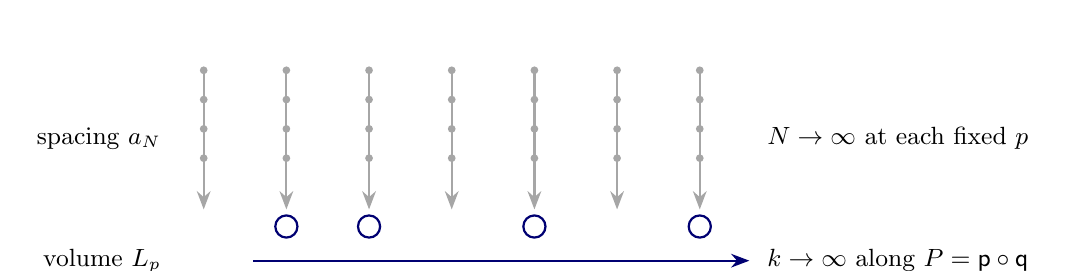
\begin{tikzpicture}[x=1.05cm,y=0.62cm,>=Stealth,font=\small]
\foreach \p in {1,...,7}{
  \draw[->,thick,gray!70] (\p,3.2) -- (\p,0.35);
  \foreach \n in {3.2,2.6,2.0,1.4}{\fill[gray!70] (\p,\n) circle (1.4pt);}
}
\foreach \p in {2,3,5,7}{\draw[thick,paperlink] (\p,0) circle (4pt);}
\draw[->,thick,paperlink] (1.6,-0.7) -- (7.6,-0.7);
\node[anchor=west] at (7.7,-0.7) {$k\to\infty$ along $P=\mathsf p\circ\mathsf q$};
\node[anchor=west] at (7.7,1.8) {$N\to\infty$ at each fixed $p$};
\node[anchor=east] at (0.6,1.8) {spacing $a_N$};
\node[anchor=east] at (0.6,-0.7) {volume $L_p$};
\end{tikzpicture}
\caption{The two limits of Definition~\ref{def:D09}. At every fixed volume the full sequence of spacings is used (vertical arrows); the volume limit then runs along the retained indices $P(k)$ (circled), chosen once for all fields and tests.}\label{fig:two-limits}
\end{figure}

\subsection{Local fields}\label{sec:local-fields}

Two examples orient this subsection. The unit label has the constant insertion one at every sufficiently fine cutoff. The curvature square $c_{F^2}=\frac14\sum_{a,b}\langle F_{ab},F_{ab}\rangle_\g$, the Yang--Mills density at a point, is read to leading order by the clover average $P^{\rm cl}=\frac14\sum_\square\wilsonterm(U_\square)$ over the $24$ plaquettes with a corner at the site: since $\wilsonterm=\frac12\chord^2$, the expansion of Section~\ref{sec:wilson} gives each of them $\frac12h_{\rm lat}^4|F_{ab}|_\g^2+O(h_{\rm lat}^5)$ for the links of a smooth field, so $P^{\rm cl}=h_{\rm lat}^4c_{F^2}+O(h_{\rm lat}^5)$ with $F$ taken at the site. The construction itself uses the local sections below, normalized by a linear map (Definition~\ref{def:D08}).

In general, local fields are labelled by invariant polynomials in the Taylor coefficients of a connection. The labels use radial, or Fock--Schwinger, gauge, in which the radial component of the connection vanishes. In this gauge a smooth connection satisfies $\mathcal A_a(x)=\int_0^1t\,x^bF_{ba}(tx)\,dt$, so its homogeneous part of degree $k+1$ is determined by the $k$th Taylor coefficients of the curvature at the origin.

\begin{definition}[Polynomial labels]\label{def:D07}
Let $\mathcal J$ consist of formal $\g$-valued arrays $\mathcal A_a(x)=\sum_{k\ge0}\mathcal A_{k,a}(x)$, with $\mathcal A_{k,a}$ homogeneous of degree $k+1$ and $\sum_a x^a\mathcal A_{k,a}(x)=0$. A coordinate of $\mathcal A_k$ has bidegree $(k+2,1)$: engineering weight $k+2$ and factor count one. Put
\begin{equation*}
V_d=\C[\mathcal J]^{\operatorname{Ad}(G)}_{\mathrm{weight}\le d}\,,
\end{equation*}
with fixed bihomogeneous bases $b_{d,i}$ of bidegree $(w_i,k_i)$, the supremum coefficient norm, conjugation and the induced $\hypercubic$ action.
\end{definition}

For instance, at $d=4$ the retained part is $\mathcal A_0+\mathcal A_1+\mathcal A_2$: for a smooth connection in radial gauge, with the curvature and its derivatives taken at the origin and repeated indices summed,
\begin{equation*}
\mathcal A_a(x)=\tfrac12x^bF_{ba}+\tfrac13x^bx^c\partial_cF_{ba}+\tfrac18x^bx^cx^e\partial_c\partial_eF_{ba}+O(|x|^4)\,,
\end{equation*}
so the labels in~$V_4$ are invariant polynomials in the curvature and its first two derivatives at the origin. Curvature has weight two and each derivative adds one; for instance $c_{F^2}$ has bidegree $(4,2)$. Three gradings play different roles below:
\begin{itemize}[nosep]
\item the engineering weight $w$ fixes the power of the spacing in the Taylor normalization~\eqref{eq:I12-section-Taylor};
\item the factor count $k$ fixes the scaling by the small-field threshold, through the operator $\factorcount b_{d,i}=k_ib_{d,i}$ and $t^{\factorcount}b_{d,i}=t^{k_i}b_{d,i}$;
\item the degree $d$ of the space $V_d$ fixes the factor $\ell_m^d$ in the transfer of insertions under blocking and the physical prefactor $a_N^{-d}$.
\end{itemize}
A polynomial of weight at most $d\le e$ lies in $V_d$ and in~$V_e$; its two insertions differ, since the normalization below depends on the degree.

Lattice holonomies are compared with smooth connection jets. For $\mathsf j=(\mathcal A_k)_k\in\mathcal J$, put $\mathcal A^{\le d}=\sum_{k+2\le d}\mathcal A_k$. The test holonomies at spacing $h_{\rm lat}$ are, on a positive link $(y,a)$ with $y\in\Z^4$,
\begin{equation}\label{eq:I12-test-holonomy}
U(h_{\rm lat},\mathsf j)(y,a)=u(1),\qquad
u'(t)=u(t)h_{\rm lat}\mathcal A_a^{\le d}(h_{\rm lat}(y+te_a)),\qquad u(0)=1_G\,,
\end{equation}
and the jet dilation is $\operatorname{sc}_{h_{\rm lat}}\mathsf j=(h_{\rm lat}^{k+2}\mathcal A_k)_k$, so that $U(h_{\rm lat},\mathsf j)=U(1,\operatorname{sc}_{h_{\rm lat}}\mathsf j)$. For a function~$O$ of the links near the origin, its \emph{Taylor map} $\taylormap_dO$ is the part of weight at most~$d$ of the Taylor series at $\mathsf j=0$ of $\mathsf j\mapsto O(U(1,\mathsf j))$. Lemma~\ref{lem:A1} constructs a \emph{local section} $\localsection{d}[\mathbf c](y;U)$, linear in $\mathbf c\in V_d$ and polynomial in the real and imaginary parts of the link entries on a fixed finite stencil $y+\Sigma_d$; it is gauge invariant, commutes with complex conjugation, is $\hypercubic$ covariant, sends $\mathbf1$ to one, and satisfies, for $0\le q\le d$,
\begin{equation}\label{eq:I12-section-Taylor}
\left.\frac{d^q}{dh_{\rm lat}^q}\localsection{d}[\mathbf c](0;U(h_{\rm lat},\mathsf j))\right|_{h_{\rm lat}=0}
=\left.\frac{d^q}{dh_{\rm lat}^q}\mathbf c(\operatorname{sc}_{h_{\rm lat}}\mathsf j)\right|_{h_{\rm lat}=0}\,.
\end{equation}
Equivalently, $\taylormap_d\localsection{d}[\mathbf c]=\mathbf c$: the local section is a right inverse of the Taylor map, which explains its name. A homogeneous label of weight $w$ specifies the coefficient of $h_{\rm lat}^w$; for example $\taylormap_4P^{\rm cl}=c_{F^2}$. Smooth connections enter only as test configurations that define and normalize lattice observables; the labels assert nothing about differentiability of a continuum field.

An \emph{insertion label} is a pair $v=(d,\mathbf c)$ with $d\in\N$ and $\mathbf c\in V_d$; the set of insertion labels is $\mathcal T=\bigsqcup_dV_d$. The insertions of the construction are normalized at a fixed physical scale. Section~\ref{sec:renormalization} fixes, for each $d$, a reference level $\reflevel{d}$, the small-field threshold $t_N$ at the cutoff~\eqref{eq:I12-scales}, and, along the trajectories of Theorem~\ref{prop:MT}, an invertible linear map $\mathsf Z_{N,p,d}$ of $V_d$, the terminal map: it sends a coefficient vector given at the cutoff to the coefficient vector of the blocked insertion at level $\reflevel{d}$ (Section~\ref{sec:marked}). For $N<\reflevel{d}$ it is a fixed invertible map.

\begin{definition}[Renormalized insertions]\label{def:D08}
For every $N,p$, $(d,\mathbf c)\in\mathcal T$ and site~$y$, put
\begin{equation*}
I_{N,p}((d,\mathbf c),y;U)=O^{(d)}_{N,p}(\mathbf c,y;U)
=a_N^{-d}\localsection{d}\bigl[t_N^{-\factorcount}\mathsf Z_{N,p,d}^{-1}\mathbf c\bigr](y;U)\,.
\end{equation*}
The unit coefficient is $\mathbf u_d=a_{\reflevel{d}}^d\mathbf1$.
\end{definition}

The inverse terminal map makes the transferred coefficient equal to the prescribed $\mathbf c$ at the reference level, so $\mathbf c$ is specified at the fixed physical scale $a_{\reflevel{d}}$, in that level's lattice units; $t_N^{-\factorcount}$ measures each factor in units of the small-field threshold, and $a_N^{-d}$ converts to physical units. Because blocking can mix labels of different weight within $V_d$, the normalization is an invertible linear map of $V_d$ rather than a factor for each label. As a first check, the insertion of $\mathbf u_d$ is the constant one for $N\ge\reflevel{d}$: the terminal map sends $a_N^d\mathbf1$ to $a_{\reflevel{d}}^d\mathbf1$ (Lemma~\ref{lem:E2.1a}), $t_N^{-\factorcount}\mathbf1=\mathbf1$, and the section sends $\mathbf1$ to one. Part~II follows the curvature square through these maps (Section~\ref{sec:A-example}); the following table summarizes the data of a smeared correlation.
\begin{center}\small
\begin{tabular}{@{}p{0.22\textwidth}p{0.3\textwidth}p{0.4\textwidth}@{}}
\toprule
\raggedright Object & \raggedright Role & \raggedright Example\tabularnewline
\midrule
\raggedright label $v=(d,\mathbf c)\in\mathcal T$ & \raggedright chooses the local measurement & \raggedright $(4,c_{F^2})$\tabularnewline
\raggedright insertion $I_{N,p}(v,y;U)$ & \raggedright its cutoff recipe on the stencil $y+\Sigma_d$ & \raggedright $a_N^{-4}\bigl(\lambda_{N,p}t_N^{-2}\localsection{4}[c_{F^2}](y;U)+\delta^{F^2}_{N,p}\bigr)$ for $N\ge\reflevel{4}$\tabularnewline
\raggedright separated test $f$ & \raggedright weights the positions in $\latsmear_{N,p}(v;f)$ & \raggedright $f_1(x_1)f_2(x_2)$, with $f_1,f_2$ of disjoint supports\tabularnewline
\bottomrule
\end{tabular}
\end{center}
Here $\lambda_{N,p}\ne0$ and $\delta^{F^2}_{N,p}$ are real; the multiple of the unit accounts for mixing of the curvature square with the constant under blocking. The trace of the holonomy around a fixed lattice loop is also continuous, gauge invariant and local on a finite stencil, but it is not thereby an insertion of the family constructed here, and no limit is asserted for loops of fixed physical size, whose stencils grow as $a_N\to0$.

\subsection{Euclidean properties}\label{sec:euclidean-properties}

A \emph{table}, or family of Schwinger functions, assigns to each degree list $(d_i)_{i=1}^n$ and $x\in\Conf{n}$ a complex multilinear function $S_n(c;x)$ of $c_i\in V_{d_i}$. For $v_i=(d_i,c_i)$ write $S_n(v;x)$, and for the word $w=(v_i(x_i))_{i=1}^n$ write $S(w)$; the product of words concatenates their lists. Conjugation and $\hypercubic$ act on labels as in Definition~\ref{def:D07}, and $h\in\hypercubic$ acts on positions linearly. Thus two insertion labels $v_1,v_2$ and two distinct points $x_1\ne x_2$ select one number $S_2(v;x_1,x_2)$, and a separated test~$f$ on~$(\R^4)^2$ selects the number $\int f(x)S_2(v;x)\,dx$. In the main theorem this number is the ordered limit~\eqref{eq:intro-ordered-limit}: the full cutoff limit at each fixed volume, then the volume limit along a refinement that may depend on the prescribed sequence~$\mathsf p$ and serves every label list and test. A table has no values on the collision diagonals. Values assigned there are invisible to separated tests (Step~\ref{step:deduction-hierarchy} of Section~\ref{sec:deduction}); a contact extension (Section~\ref{sec:short-distance-defs}) is instead a distribution on all of~$(\R^4)^n$ that agrees with the table on separated tests, and Theorem~\ref{prop:CT} constructs one.

\begin{definition}[E1--E3. Euclidean symmetries]\label{def:E1-E3}
For every $n$, degree list, $c$ and $x\in\Conf{n}$:
\begin{enumerate}[label=\textup{(E\arabic*)},ref=E\arabic*,nosep]
\item\label{it:E1} $S_0=1$, $S_n(c_\pi;x_\pi)=S_n(c;x)$ for every permutation $\pi$ of the slots, and $S_{n+1}(\mathbf u_d,c;x_0,x)=S_n(c;x)$;
\item\label{it:E2} $S_n(hc;hx)=S_n(c;x)$ for $h\in\hypercubic$, and $S_n(\bar c;x)=\overline{S_n(c;x)}$;
\item\label{it:E3} $S_n(c;x+z)=S_n(c;x)$ for $z\in\R^4$, with $x+z=(x_i+z)_i$.
\end{enumerate}
\end{definition}

A word is positive-side for the axis~$a$ when all its positions have positive $a$th coordinate. For a word $w$, let $\theta_aw=\mathsf s_a^{\rm refl}(w^*)$, where $w^*$ reverses the word and applies conjugation to its labels, and $\mathsf s_a^{\rm refl}$ reflects positions and acts on labels through~$\hypercubic$.

\begin{definition}[E4--E5. Reflection positivity]\label{def:E4-E5}
\begin{enumerate}[label=\textup{(E\arabic*)},ref=E\arabic*,start=4,nosep]
\item\label{it:E4} For every axis~$a$, positive-side separated words~$w_i$ and $z_i\in\C$, $\sum_{i,j}\bar z_iz_jS(\theta_a(w_i)\,w_j)\ge0$.
\item\label{it:E5} The same positivity holds for finite sums of words smeared against joint smooth compactly supported tests on positive-side separated configurations, and every mixed pairing is absolutely integrable.
\end{enumerate}
\end{definition}

For a fixed label list, $D_x^k$ is the $k$th Fr\'echet derivative in the positions, with the product Euclidean norm. The last condition controls the approach to collisions uniformly over translations and over configurations of large diameter.

\begin{definition}[E6--E7. Euclidean regularity]\phantomsection\label{def:E6-E7}
\begin{enumerate}[label=\textup{(E\arabic*)},ref=E\arabic*,start=6,nosep]
\item\label{it:E6} Each $S_n(c;\cdot)$ is smooth on~$\Conf{n}$.
\item\label{it:E7} For all $n,d,c,k$ there are $C(n,d,c,k)\ge0$ and an integer $A(n,d,c,k)\ge0$ such that $\|D_x^kS_n(c;x)\|\le Cr^{-A}$ whenever $0<r\le1$ and $\sepinf(x)\ge r$.
\end{enumerate}
\end{definition}

\subsection{Field spaces and phases}\label{sec:field-spaces}

A field is described in three successive ways. An insertion label $(d,c)$ specifies a lattice insertion. Its class $[c]$ identifies labels with the same separated correlations: two labels represent the same field when every spectator sees the same answer. The response $\iota_d[c]$ records those correlations against every spectator list and places fields of all degrees in one space. Write $v(x)=(v_1(x_1),\ldots,v_n(x_n))$ for a spectator word.

\begin{definition}[Observable fields]\label{def:D10}
For a table~$S$ put
\begin{align*}
\nullspace{d}(S)&=\bigl\{c\in V_d:S_{n+1}(c(x_0),v(x))=0\text{ for every }n,v\text{ and }(x_0,x)\in\Conf{n+1}\bigr\},\\
F_d&=V_d/\nullspace{d}(S),\qquad \overline{[c]}=[\bar c],\qquad h[c]=[hc]\quad(h\in\hypercubic),\\
\iota_d[c](v;x_0,x)&=S_{n+1}(c(x_0),v(x)),\qquad
\mathcal L=\operatorname{span}\bigcup_d\iota_dF_d\,,
\end{align*}
with conjugation-invariant quotient norms on the finite-dimensional spaces~$F_d$.
\end{definition}

By~\ref{it:E2}, $\nullspace{d}(S)$ is invariant under conjugation and~$\hypercubic$, so both actions on $F_d$ are well defined. By~\ref{it:E1}, correlations do not depend on representatives in any slot: for $\boldsymbol A=([c_1],\ldots,[c_n])$ put $S_n(\boldsymbol A;x)=S_n(c;x)$. The unit field is $\unitfield{d}=[\mathbf u_d]$. Write $\mathbb F=\bigsqcup_dF_d$, $\deg(d,A)=d$ and $\iota(d,A)=\iota_dA$; the elements of $\mathcal L$ are the field labels.

\paragraph{Phases.}
The main theorem writes the limiting table as an average $S=\int_{\phases}S^\xi\,d\nu(\xi)$ of tables $S^\xi$ on the same field spaces, over a compact metric space $\phases$ with a fully supported probability measure~$\nu$; the points~$\xi$ are the phases. A phase is not a set of configurations: Section~\ref{sec:phases} obtains the phases as the characters of a commutative algebra of operators.

\subsection{Wightman theories}\label{sec:wightman-defs}

Write $\mathcal S_n=\mathcal S(\R^{4n};\C)$ for the Schwartz space and $\mathcal S=\mathcal S_1$. Let $\mathcal P=SO^+(1,3)\ltimes\R^4$ be the proper orthochronous Poincar\'e group, where $SO^+(1,3)$ consists of the linear maps of determinant one that preserve $\minksquare$ and $\forwardcone$; write $\gamma=(\Lambda_\gamma,z_\gamma)$ and $(\gamma\cdot f)(x)=f(\Lambda_\gamma^{-1}(x-z_\gamma))$.

\begin{definition}[Relativistic datum]\label{def:D14a}\label{def:D14b}
A relativistic datum consists of a complex Hilbert space $\mathcal H$, a complex vector space $\mathcal L$ of field labels, a linear subspace $\mathcal D\subset\mathcal H$, a vacuum $\Omega\in\mathcal D$, and fields $\Phi(\ell,f):\mathcal D\to\mathcal D$, linear operators that are complex bilinear in $(\ell,f)\in\mathcal L\times\mathcal S$; an antilinear map $\ell\mapsto\ell^*$; strongly continuous unitary translations $\mathsf T(z)$, $z\in\R^4$; a Borel projection-valued measure $\mathsf E$ on~$\R^4$ with finite diagonal measures $\mu_\psi(B)=\langle\psi,\mathsf E(B)\psi\rangle$; a strongly continuous unitary representation $\mathsf U$ of~$\mathcal P$ with $\mathsf U(1,z)=\mathsf T(z)$; and linear bijections $\rho_{\rm lab}(\gamma)$ of~$\mathcal L$.
\end{definition}

\begin{definition}[Wightman theory]\label{def:wightman}
A relativistic datum is a Wightman theory if:
\begin{enumerate}[label=\textup{(W\arabic*)},ref=W\arabic*,start=0,nosep]
\item\label{def:W0} $\langle\psi,\mathsf T(z)\psi\rangle=\int e^{i\mathbf p\cdot z}\,d\mu_\psi(\mathbf p)$ for all $\psi,z$, with the Euclidean pairing; $\mathsf E(\R^4\setminus\forwardcone)=0$; and every vector fixed by all translations lies in $\C\Omega$.
\item\label{def:W1} $\|\Omega\|=1$; $\mathcal D$ is dense and spanned by the vectors $\Phi(\ell_1,f_1)\cdots\Phi(\ell_k,f_k)\Omega$, $k\ge0$; each $f\mapsto\Phi(\ell,f)\psi$ is continuous from $\mathcal S$ to~$\mathcal H$; and $\langle\Phi(\ell,f)\psi,\chi\rangle=\langle\psi,\Phi(\ell^*,\bar f)\chi\rangle$ for $\psi,\chi\in\mathcal D$.
\item\label{def:W2} $\rho_{\rm lab}$ is a representation; $\mathsf U(\gamma)\mathcal D\subset\mathcal D$, $\mathsf U(\gamma)\Omega=\Omega$ and $\mathsf U(\gamma)\Phi(\ell,f)\psi=\Phi(\rho_{\rm lab}(\gamma)\ell,\gamma\cdot f)\mathsf U(\gamma)\psi$ for $\psi\in\mathcal D$.
\item\label{def:W3} $[\Phi(\ell,f),\Phi(\ell',h)]\psi=0$ for $\psi\in\mathcal D$ whenever $\minksquare(x-y)<0$ for all $x\in\operatorname{supp}f$, $y\in\operatorname{supp}h$.
\end{enumerate}
\end{definition}

\begin{definition}[Faithful labels]\label{def:D14c}
The labels are faithful if, for every nonzero $\ell\in\mathcal L$, some $f\in\mathcal S$ has $\Phi(\ell,f)\ne0$.
\end{definition}

Reconstruction uses one function in two limits: at imaginary times it equals the Euclidean correlation, and approaching real times from the ordered tube gives the Wightman distributions. We first specify the continuation, then its boundary value.

\begin{definition}[Ordered-time continuation]\label{def:D15}
For a phase~$\xi$, put $\mathcal Z_n=\{z\in\C^n:\operatorname{Im}z_1<\cdots<\operatorname{Im}z_n\}$. A continuation $\mathsf F_n^\xi(\boldsymbol A;z,\vec x)$, for $\boldsymbol A\in\mathbb F^n$, is holomorphic in $z\in\mathcal Z_n$ at each fixed real spatial configuration and satisfies
\begin{equation*}
\mathsf F_n^\xi(\boldsymbol A;(it_i)_i,\vec x)=S_n^\xi(\boldsymbol A;(\vec x_i,t_i)_i)\qquad(t_1<\cdots<t_n)\,.
\end{equation*}
\end{definition}

\begin{definition}[Boundary condition]\label{def:D14f}
For a phase $\xi$, a relativistic datum $(\mathcal H_\xi,\mathcal L,\mathcal D_\xi,\Omega_\xi,\Phi_\xi,\ldots)$, the maps $\iota_d$ and a continuation $\mathsf F_n^\xi$, require, for every $n$, $\boldsymbol A\in\mathbb F^n$, real $h_1<\cdots<h_n$ and $f_i\in\mathcal S$, that the integrand below be integrable for every $r>0$ and
\begin{multline*}
\lim_{r\downarrow0}\int\mathsf F_n^\xi(\boldsymbol A;(x_i^4+irh_i)_i,(\vec x_i)_i)\prod_i f_i(x_i)\,dx\\
=\langle\Omega_\xi,\Phi_\xi(\iota(A_1),f_1)\cdots\Phi_\xi(\iota(A_n),f_n)\Omega_\xi\rangle\,.
\end{multline*}
\end{definition}

A phase $S^\xi$ is the \emph{Euclidean continuation} of a Wightman theory when continuations satisfying Definitions~\ref{def:D15} and~\ref{def:D14f} exist for that theory and the response maps of Definition~\ref{def:D10}.

\subsection{The trace and product statements}\label{sec:short-distance-defs}

For a phase $\xi$ and a field $\Theta\in F_4$, the time-axis two-point function is
\begin{equation*}
\tracetwopoint(r)=S_2^{\xi}(\Theta,\Theta;-re_4/2,re_4/2)\qquad(r>0)\,.
\end{equation*}
The trace law is compared with free fields through the following class. Fix $m_{\rm sh}\ge0$, integers $j_h,k_E\ge0$ and a continuous real $h_{\rm mom}$ on $\R^3$ with $h_{\rm mom}(t\mathbf k)=t^{j_h}h_{\rm mom}(\mathbf k)$ for $t>0$.

\begin{definition}[Finite Wick profiles]\label{def:D17}
Put $\omega_{m_{\rm sh}}(\mathbf k)=\sqrt{m_{\rm sh}^2+|\mathbf k|^2}$ and, for $r>0$,
\begin{equation*}
K_{m_{\rm sh},k_E,h_{\rm mom}}(r)=\int_{\R^3}\frac{\omega_{m_{\rm sh}}(\mathbf k)^{k_E}h_{\rm mom}(\mathbf k)}{2\omega_{m_{\rm sh}}(\mathbf k)}e^{-r\omega_{m_{\rm sh}}(\mathbf k)}\,d^3\mathbf k\,.
\end{equation*}
A finite Wick profile is a function $W_{\rm Wick}(r)=\sum_{i=1}^{N}c_i\prod_{j=1}^{n_i}K_{m_{ij},k_{ij},h_{ij}}(r)$, $r>0$, with $c_i\in\C$ and finitely many terms and factors of this kind; empty products are one.
\end{definition}

The momentum integrals converge absolutely for $r>0$. For a free scalar field of mass $m_{\rm sh}$ the time-axis two-point function is $(2\pi)^{-3}K_{m_{\rm sh},0,1}(r)$; derivatives give momentum factors, and Wick contractions give finite sums of products at the same radius.

The product expansion replaces a cluster of nearby fields by fields at one point, inside correlations with distant spectators. For finite index sets $I_{\rm cl},I_{\rm sp}$, write $S^\zeta(\boldsymbol A,x;\boldsymbol B,y)$ for the correlation of the concatenated lists, in a fixed enumeration of $I_{\rm cl}\sqcup I_{\rm sp}$, where $\zeta\in\phases\sqcup\{\mathrm{mix}\}$ indexes a phase or the mixture, $S^{\rm mix}=S$. A pair $(x,o)$, with $x\in(\R^4)^{I_{\rm cl}}$ and $o\in\R^4$, is an $(r,M_{\rm geo},\eta)$-cluster if $|x_i-o|\le M_{\rm geo}r$ and $|x_i-x_{i'}|\ge\eta r$ for distinct slots; spectators $y\in(\R^4)^{I_{\rm sp}}$ are $\delta_{\rm sp}$-clear if $|o-y_j|\ge\delta_{\rm sp}$ and $|y_j-y_{j'}|\ge\delta_{\rm sp}$ for distinct slots. The expansion uses finite channel sets $\channels{j}$, real fields $O_{j,\lambda}\in F_j$ forming bases of conjugation-invariant complements of $F_{j-1}$ in $F_j$ ($F_{-1}=0$), and coefficient functions $c_{j,\lambda}(\boldsymbol A;x,o)$, all fixed once before spectators, states and truncations; Section~\ref{sec:trace-products} describes how they are read off. Put $|\boldsymbol A|_{\deg}=\sum_i\deg A_i$.

\begin{definition}[Product remainder]\label{def:D18}
For $D\in\N$, $\boldsymbol A\in\mathbb F^{I_{\rm cl}}$ and $\boldsymbol B\in\mathbb F^{I_{\rm sp}}$, put
\begin{equation*}
\mathcal R_D^\zeta=S^\zeta(\boldsymbol A,x;\boldsymbol B,y)-\sum_{j=0}^D\sum_{\lambda\in\channels{j}}c_{j,\lambda}(\boldsymbol A;x,o)S^\zeta(O_{j,\lambda}(o),\boldsymbol B(y))\,.
\end{equation*}
\end{definition}

If $M_{\rm geo}r<\delta_{\rm sp}$, the concatenated positions are separated, $|x_i-y_j|\ge\delta_{\rm sp}-M_{\rm geo}r>0$, so the remainder is defined in the small-radius range used below. A \emph{contact extension} of $S_n^\zeta(\boldsymbol A;\cdot)$ is a distribution on $\R^{4n}$ whose value on every separated test~$f$ is $\int f(x)S_n^\zeta(\boldsymbol A;x)\,dx$; Theorem~\ref{prop:CT} constructs one by an explicit subtraction.

\section{The main theorem}\label{sec:main-theorem}\label{sec:main-theorems}

The main theorem concerns one Wilson family~$\mathcal W$, fixed before any sequence of volumes is prescribed: the renormalized insertions of Definition~\ref{def:D08} on the bare couplings of the multiscale theorem (Theorem~\ref{prop:MT}), for a fixed block penalty. These couplings are tuned, volume by volume, so that the running coupling reaches one common endpoint coupling~$\bar\beta$ at the unit scale (Section~\ref{sec:trajectories}). Clause~(ii) also packages the objects of clauses~(iii)--(v) as hierarchy data satisfying the conditions Q2--Q6 (Section~\ref{sec:correspondence}); there $\nu$ is the measure of the phase decomposition (Theorem~\ref{prop:PH}), $\xi_*$ the selected phase (Section~\ref{sec:phases}) and $\Theta$ the centered stress trace (Definition~\ref{def:D16}), and Section~\ref{sec:deduction} assembles the hierarchy data from these objects.

The conclusions below depend on the unresolved estimates and convergence inputs listed in \hyperref[par:proof-status]{the proof-status notice}. Their proofs are conditional on those inputs.

\setcounter{maintheorem}{1}
\begin{maintheorem}[Main theorem]\label{thm:B}
For every gauge group~$G$ of Definition~\ref{def:D01} and~$\blockpenalty>0$, the renormalized insertions (Definition~\ref{def:D08}) on the penalty-$\blockpenalty$ trajectories of Theorem~\ref{prop:MT} form a regular Wilson family~$\mathcal W$ with $a_N\downarrow0$, $L_p\uparrow\infty$ and $\beta_{N,p}/\log(1/a_N)\to\slope$ uniformly in~$p$. Moreover:
\begin{enumerate}[label=\textup{(\roman*)},ref=\roman*]
\item\label{it:B1} For every~$p$, $v\in\mathcal T^n$ and $p$-admissible separated~$f$, $\latsmear_{N,p}(v;f)\to\int fM^{\rm UV}_{p,v}$ as $N\to\infty$.
\item\label{it:B2} For every strictly increasing~$\mathsf p$ there are a strictly increasing~$\mathsf q$, a table~$S$ satisfying E1--E7 and hierarchy data over~$\mathcal W$ satisfying Q2--Q6 with $\mathcal W\to S$ and $\mathcal W\to S^{\rm mix}\circ\pi_{\rm quo}$ along~$P=\mathsf p\circ\mathsf q$. In (iii)--(v), $S$ is this table, $F_d=V_d/\nullspace{d}(S)$, and $\nu$, $\xi_*$, $\Theta$ are those of these hierarchy data.
\item\label{it:B3} $S=\int_{\phases}S^\xi\,d\nu(\xi)$ with $\nu$ a fully supported probability measure on a compact metric space; each~$S^\xi$ is the Euclidean continuation of a faithful Wightman theory with unique vacuum.
\item\label{it:B4} A conserved stress tensor is normalized by its shell fluxes (Theorem~\ref{prop:ST}); in the selected phase~$\xi_*$ its centered trace~$\Theta$ has
\begin{equation*}
r^8\log^2(1/r)\tracetwopoint(r)\to3\dimG/\pi^4,
\end{equation*}
and $\tracetwopoint$ agrees with no finite Wick profile on any interval~$(0,\delta)$.
\item\label{it:B5} The fields~$F_d$ have an operator product expansion with spectator-independent coefficients and
\begin{equation*}
|\mathcal R_D^\zeta|\le r^{D+1-|\boldsymbol A|_{\deg}-\varepsilon},
\end{equation*}
with the quantifiers and uniformity of Theorem~\ref{prop:OP}, and contact extensions from the same prescription.
\end{enumerate}
\end{maintheorem}

The kernel $M^{\rm UV}_{p,v}$ of clause~(i) is the fixed-volume limit of Theorem~\ref{prop:UV}, the convergence $\mathcal W\to S$ in clause~(ii) is that of Definition~\ref{def:D09}, and $\pi_{\rm quo}(d,\mathbf c)=(d,[\mathbf c])$ sends an insertion label to its field. Section~\ref{sec:deduction} deduces the theorem from the principal results of Sections~\ref{sec:renormalization} and~\ref{sec:continuum-results}, subject to the stated proof inputs.

\paragraph{Order of choices.}
The gauge group, its realization and the block penalty are fixed first. The lattice family, with its couplings and insertions, is then fixed before the volume sequence~$\mathsf p$. The refinement~$\mathsf q$, the table~$S$, the field spaces, the phases, the selected phase, the relativistic theories, the product coefficients and the trace field may depend on~$\mathsf p$. One refinement serves every arity, every list of insertion labels and every separated test. The lattice limit in clause~(ii) is the mixture~$S$; the relativistic theories of clause~(iii) belong to the phases, and the trace law of clause~(iv) is stated in the selected phase.

\paragraph{What the theorem does not assert.}
It does not prove a mass gap, that is, a positive lower bound on the nonzero energies; uniqueness of the vacuum means only that the zero-energy space is one-dimensional, and no clause excludes nonzero energies accumulating at zero. It does not assert that the infinite-volume limit, the phase space or the selected phase is unique, nor that different block penalties give the same theory, and it does not take the spacing and volume limits simultaneously. It does not show that widely separated groups of observations become independent in the mixed state, or that any one phase is itself a limit of lattice states. The lattice correlations converge against separated tests; the contact extensions are constructed afterwards from the separated correlations, are not limits of unsubtracted lattice correlations at coincident points, and are not asserted to be unique, positive or to satisfy contact Ward identities. The product expansion is an estimate at each finite truncation degree, not the convergence of a series as that degree tends to infinity. The trace law is asserted in the selected phase only, and it excludes the finite Wick profiles of Definition~\ref{def:D17}; a generalized free field with the spectral measure of~$\Theta$ has the same two-point function.

Section~\ref{sec:correspondence} states Theorem~\ref{thm:A}, a weaker existence statement with conditions Q0--Q6, and deduces it from Theorem~\ref{thm:B} with any $\blockpenalty>0$.

\section{Strategy of the proof}\label{sec:strategy}\label{sec:intro-outline}

The proof fixes one lattice family, takes its two limits and identifies the resulting fields; every estimate applies to this same family. Figure~\ref{fig:dependency} shows the order in which the principal results use one another. This section explains the mechanisms that make the main steps work; Sections~\ref{sec:renormalization}--\ref{sec:continuum-results} state the results with the ideas of their proofs.

\begin{figure}[ht]
\centering
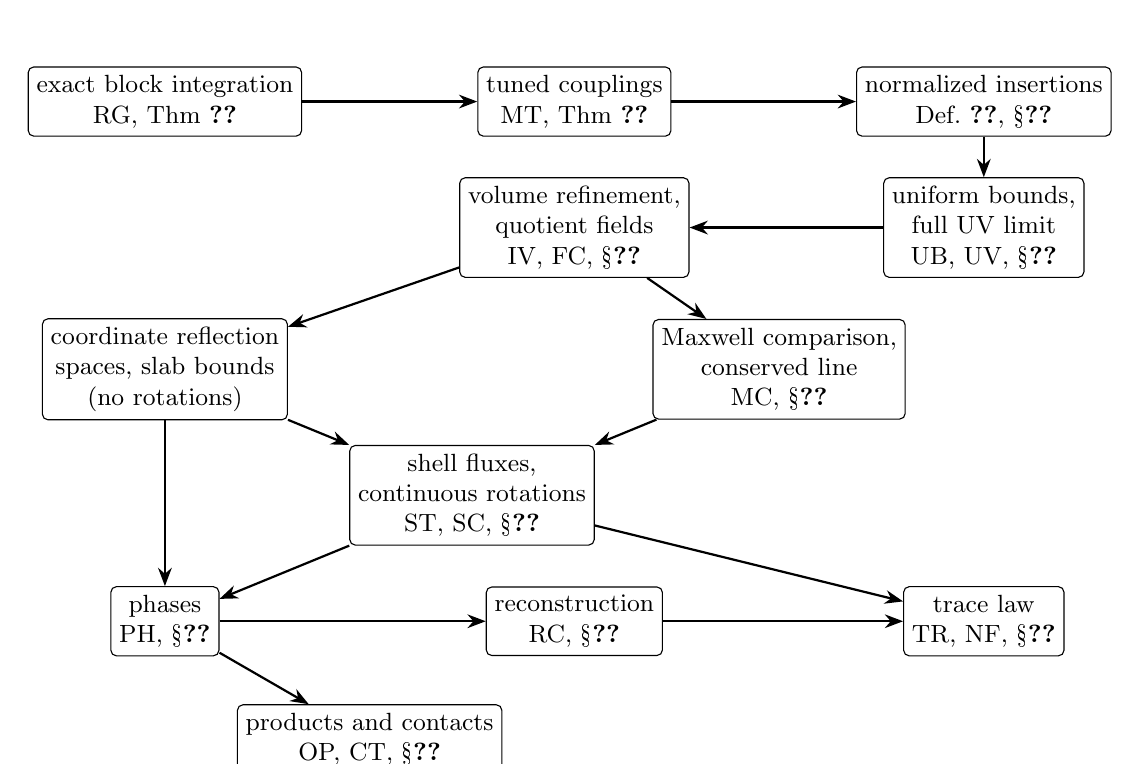
\begin{tikzpicture}[>=Stealth,font=\small,
  box/.style={draw,rounded corners=2pt,align=center,inner sep=3pt,fill=white},
  ar/.style={->,thick}]
\node[box] (rg) at (0,0) {exact block integration\\ RG, Thm~\ref{prop:RG}};
\node[box] (mt) at (5.2,0) {tuned couplings\\ MT, Thm~\ref{prop:MT}};
\node[box] (ins) at (10.4,0) {normalized insertions\\ Def.~\ref{def:D08}, \S\ref{sec:marked}};
\node[box] (uv) at (10.4,-1.6) {uniform bounds,\\ full UV limit\\ UB, UV, \S\ref{sec:uv-limit}};
\node[box] (iv) at (5.2,-1.6) {volume refinement,\\ quotient fields\\ IV, FC, \S\ref{sec:volume-limit}};
\node[box] (os) at (0,-3.4) {coordinate reflection\\ spaces, slab bounds\\ (no rotations)};
\node[box] (mc) at (7.8,-3.4) {Maxwell comparison,\\ conserved line\\ MC, \S\ref{sec:stress}};
\node[box] (st) at (3.9,-5.0) {shell fluxes,\\ continuous rotations\\ ST, SC, \S\ref{sec:stress}};
\node[box] (ph) at (0,-6.6) {phases\\ PH, \S\ref{sec:phases}};
\node[box] (rc) at (5.2,-6.6) {reconstruction\\ RC, \S\ref{sec:phases}};
\node[box] (tr) at (10.4,-6.6) {trace law\\ TR, NF, \S\ref{sec:trace-products}};
\node[box] (op) at (2.6,-8.1) {products and contacts\\ OP, CT, \S\ref{sec:trace-products}};
\draw[ar] (rg) -- (mt); \draw[ar] (mt) -- (ins); \draw[ar] (ins) -- (uv); \draw[ar] (uv) -- (iv);
\draw[ar] (iv) -- (os); \draw[ar] (iv) -- (mc);
\draw[ar] (os) -- (st); \draw[ar] (mc) -- (st);
\draw[ar] (st) -- (ph); \draw[ar] (os) -- (ph); \draw[ar] (ph) -- (rc);
\draw[ar] (st) -- (tr); \draw[ar] (rc) -- (tr);
\draw[ar] (ph) -- (op);
\end{tikzpicture}
\caption{Dependency map. An arrow means that the later result uses the earlier one; the trace law and the products branch off the main route. The coordinate reflection spaces and slab bounds use only the volume limit and the field calculus; they enter the rotation argument before continuous rotations are available, so the order is not circular. The renormalization group runs only from the cutoff to the unit scale, and no mass gap is used.}\label{fig:dependency}
\end{figure}

\subsection{Why the ultraviolet induction closes}\label{sec:closes}

Blocking integrates the fine links against a probability kernel and returns an exact density for the coarse links (Definition~\ref{def:D04}); it lowers the level from $m+1$ to $m$ and multiplies the spacing by the odd block ratio $\ell_m$ (Figures~\ref{fig:scales} and~\ref{fig:rg-block-step}). The density is written as a curvature action with the running coupling $\beta_m$, a scalar normalization, regular activities on small-field supports and forced activities covering every large-field site (Section~\ref{sec:density}). The equality is exact; the estimates control the coordinates in which it is written. Five points make the induction close.

\begin{figure}[ht]
\centering
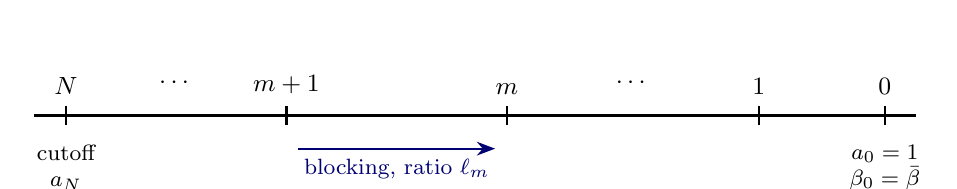
\begin{tikzpicture}[>=Stealth,font=\small,x=1cm,y=1cm]
\draw[thick] (0,0) -- (11.2,0);
\foreach \x/\l in {0.4/N,3.2/m+1,6.0/m,9.2/1,10.8/0}{\draw[thick] (\x,-0.12) -- (\x,0.12); \node[above] at (\x,0.15) {$\l$};}
\node at (1.8,0.42) {$\cdots$}; \node at (7.6,0.42) {$\cdots$};
\draw[->,thick,paperlink] (3.35,-0.42) -- node[below,font=\footnotesize]{blocking, ratio $\ell_m$} (5.85,-0.42);
\node[below,font=\footnotesize,align=center] at (0.4,-0.25) {cutoff\\$a_N$};
\node[below,font=\footnotesize,align=center] at (10.8,-0.25) {$a_0=1$\\$\beta_0=\bar\beta$};
\end{tikzpicture}
\caption{Levels and the direction of integration. Level $m$ has spacing $a_m=D_m^{-1}$; blocking runs from the fine level $m+1$ to the coarse level $m$, so $a_{m+1}<a_m$, and the running coupling decreases by about $\slope\log\ell_m$, so $\beta_{m+1}>\beta_m$ to leading order. The ratios grow: $\log\ell_m\to\infty$ and $\log\ell_m/\log D_m\to0$. The endpoint coupling $\bar\beta$ is prescribed at level zero, the reference unit of length, which is not a measured mass scale.}\label{fig:scales}
\end{figure}

\begin{figure}[ht]
\centering
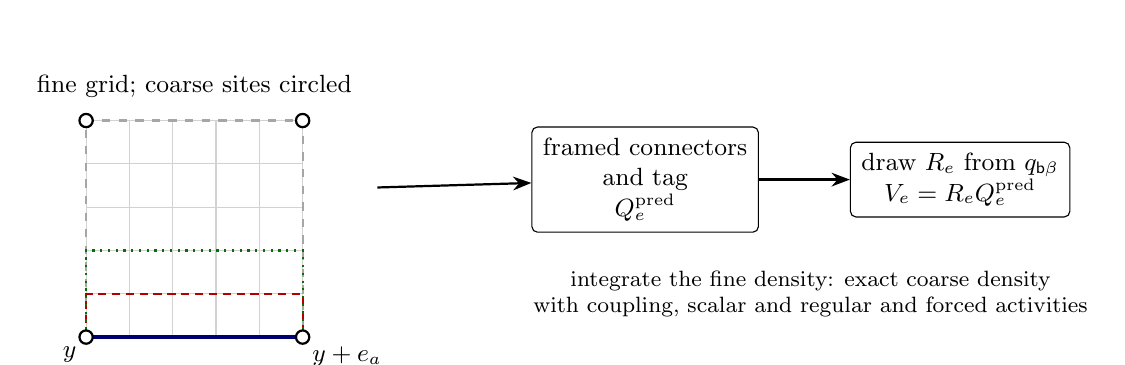
\begin{tikzpicture}[>=Stealth,font=\small,
  box/.style={draw,rounded corners=2pt,align=center,inner sep=4pt},
  ar/.style={->,thick}]
% A two-dimensional schematic of fine links and one coarse edge.
\begin{scope}[x=0.55cm,y=0.55cm]
  \draw[step=1,gray!35,thin] (0,0) grid (5,5);
  \draw[gray!70,dashed,thick] (0,0) -- (0,5) -- (5,5) -- (5,0);
  \draw[paperlink,very thick] (0,0) -- (5,0);
  \draw[red!70!black,thick,densely dashed] (0,0) -- (0,1) -- (5,1) -- (5,0);
  \draw[green!45!black,thick,dotted] (0,0) -- (0,2) -- (5,2) -- (5,0);
  \foreach \x/\y in {0/0,5/0,0/5,5/5}
    \filldraw[fill=white,draw=black,thick] (\x,\y) circle (2.4pt);
  \node[below left] at (0,0) {$y$};
  \node[below right] at (5,0) {$y+e_a$};
  \node[above,align=center] at (2.5,5.3) {fine grid; coarse sites circled};
\end{scope}
\node[box] (predict) at (7.1,2.0) {framed connectors\\and tag\\$Q^{\rm pred}_e$};
\node[box] (draw) at (11.1,2.0) {draw $R_e$ from $q_{\blockpenalty\beta}$\\$V_e=R_eQ^{\rm pred}_e$};
\draw[ar] (3.7,1.9) -- (predict);
\draw[ar] (predict) -- (draw);
\node[align=center,font=\footnotesize] at (9.2,0.55) {integrate the fine density: exact coarse density\\with coupling, scalar and regular and forced activities};
\end{tikzpicture}
\caption{One block step, shown in a two-dimensional slice. The three routes schematically represent fine transports aligned at the endpoints of one highlighted coarse edge; the actual offset connectors, frames and fallback frame or connector branches are specified in Section~\ref{sec:renormalization}. Given the fine configuration and tag, the draw uses the normalized density $q_{\blockpenalty\beta}$ around the predictor. Integrating the fine links gives the exact coarse density; the activity bounds require the inputs in the proof-status notice. The spacing changes from $a_{m+1}$ to $a_m=\ell_m a_{m+1}$.}\label{fig:rg-block-step}
\end{figure}


\paragraph{One coupling to tune.}
In the local radial-gauge expansion of a gauge-invariant local term (Sections~\ref{sec:partII-C}--\ref{sec:partII-D}), the contributions of engineering weight at most four are a constant, terms linear in the curvature and its derivatives, and a quadratic curvature term. The constant goes into the scalar normalization. The linear terms vanish, since an $\operatorname{Ad}(G)$-invariant linear function on the simple algebra~$\g$ is zero; in particular there is no mass term. Simplicity of~$\g$ and the hypercubic and reflection symmetries leave one invariant quadratic curvature term, whose coefficient the construction moves into the coupling. The regular activities that remain vanish at the flat configuration and, on supports that do not wrap around the torus, have zero Hessian along affine directions (Definition~\ref{def:D24}). This subtraction plays the role of the localization operator of Bauerschmidt, Brydges and Slade~\cite[\S5.2]{BauerschmidtBrydgesSlade2019}.

\paragraph{The scales.}
Write, at one level, $b=\refbeta_m$ for the reference coupling, $M=\exp((\log\log b)^2)=(\log b)^{\log\log b}$, which grows faster than every power of $\log b$ and slower than every power of~$b$, the small-field threshold $t=b^{-1/2}M$ and the regular activity bound $\varepsilon=b^{-11/10}$ (equation~\eqref{eq:I12-scales}). Plaquette fluctuations at coupling~$b$ have size $b^{-1/2}$, so $t$ is that size enlarged by~$M$, and $t\to0$. The comparisons that fix these choices are, for $\beta\asymp b$:
\begin{center}\small
\begin{tabular}{@{}p{0.3\textwidth}p{0.63\textwidth}@{}}
\toprule
Comparison & Consequence\\
\midrule
$\beta t^5\asymp b^{-3/2}M^5=o(\varepsilon)$ & the Wilson energy matched through fourth order leaves a regular error below the bound\\
$t^3/\varepsilon=b^{-2/5}M^3\to0$ & a cubic term with bounded coefficient at the threshold is below the bound\\
$\varepsilon/t^2=b^{-1/10}M^{-2}\to0$ & a quadratic term at the threshold does not: residual quadratic coefficients go into the coupling\\
$\beta t^2\asymp M^2$ & a plaquette above the threshold costs a factor of order $e^{-cM^2}$, which is $o(b^{-k})$ for every fixed~$k$\\
\bottomrule
\end{tabular}
\end{center}
The forced activity bound $e^{-M^{1/5}}$ is $o(b^{-k})$ for every fixed~$k$ but much larger than $e^{-cM^2}$; this leaves room for the combinatorial losses of the forced terms.

\paragraph{The cancellations.}
Two cancellations make the regular bound contract. First, an incoming regular activity, written in the coarse field, loses its constant, linear and affine quadratic terms by flat normalization, colour invariance and the affine Hessian condition; the remaining terms of its principal part carry at least $\ell_m^{-5}$ (on large supports after conversion of the support weight), against $\ell_m^4$ fine anchors above a coarse anchor, a net factor $V_j/\ell_m$ with $V_j$ fixed before the ratio, while the comparison remainder has relative size $b'^{-1/2+o(1)}$, where $b'=\refbeta_{m+1}$ is the reference coupling of the fine level (Lemma~\ref{lem:D-inherited}). Second, the new terms produced by the integration are connected local terms whose bound from the connected expansion is only $P_j(b')b'^{-7/16}$ (Lemma~\ref{lem:D-connected}), where $j=J_{m+1}$ and $P_j$ denotes functions of subpower growth fixed with the stage; this is far above the required bound $\refbeta_m^{-11/10}$. Most of these terms are already small enough: the connected expansion still converges when every elementary factor is weighted by $b'^{3/8}$, so terms with three or more factors, or with a large-field overlap, are at most $P_j(b')b'^{-19/16}\le b'^{-23/20}$, and long paths, large supports and products with an incoming activity also stay below $b'^{-23/20}$. 

\paragraph{Localizing the cancellations.}
For the remaining terms, estimates of sums over reflected tori yield a bound on a local function. In four dimensions a fourth finite difference cancels the boundary classes of those sums and retains the interior contribution. Section~\ref{sec:partII-D} selects a finite family of low-order connected terms (at most two connected products of at most two factors, short paths, no incoming activity), invariant under translations and~$\hypercubic$; the unselected low-order terms have weighted norm at most $\varepsilon_{\rm tr}$; every complete read support of these terms, relative to a site receiving a share, lies within distance~$R$ of that site. Let $F_y$ be the sum of the shares at the site~$y$, a connected term being shared equally among the sites of its support and a path term assigned to its anchor. For a radius $w>4R$ fixed in Section~\ref{sec:partII-D}, with $2(w+5)$ less than the side of~$\Lambda$ by the period requirements of Section~\ref{sec:constants}, let $\Lambda_i$ be the torus of side $2(w+i)$, $i=0,\ldots,4$, let $V_{i,x}$ be the configuration on $\Lambda_i$ obtained by folding each coordinate into $x+[0,w+i]^4$, reversing bond orientations as needed, let $F^{(i)}_y$ be the same local formula on~$\Lambda_i$ with its flat value subtracted, and put
\begin{equation}\label{eq:five-torus}
\lambda_i=\frac{(-1)^i\binom4i}{2^4\,4!},\qquad
G_x=\sum_{i=0}^4\lambda_i\sum_{y\in\Lambda_i}F^{(i)}_y(V_{i,x})\,.
\end{equation}

\begin{lemma}[Five-torus localization]\label{lem:five-torus}
For the selected low-order family, the function $G_x$ depends only on the links within distance $w+5$ of~$x$, and, in the local derivative seminorm of Definition~\ref{def:D05a},
\begin{equation*}
\|G_x\|_m\le P_j(b')\bigl(b'^{-23/20}+\varepsilon_{\rm tr}\bigr).
\end{equation*}
On configurations without large-field sites, $\sum_yF_y=c|\Lambda|+\sum_xG_x$ for a constant~$c$.
\end{lemma}

This is Lemma~\ref{lem:D-localization}, which also controls the correction near large-field sites. Two facts give it. On each auxiliary torus the total of the selected family is, up to the omitted terms, a normalized local integral, in which the flat value, the classical cubic and quartic terms and the one-loop quadratic term are subtracted exactly and Gaussian parity removes a lone cubic term; what remains has at least three factors of size $b'^{-1/2+o(1)}$ or a further Taylor gain. To recover a local function from totals, classify the sites of $\Lambda_i$ by their distances through the read radius~$R$ from the reflection faces and by their local fold slopes, including wrapped neighbours. These data fix the offsets $\phi_i(y+u)-\phi_i(y)$ on the read support. Evaluate the summand at~$y$ on $V_{i,x-\phi_i(y)}$, where $\phi_i(y)_a=\min\{t_a,2(w+i)-t_a\}$ for the least residue $t_a$ modulo $2(w+i)$. This shift appears only after reindexing the sum over~$x$; in~\eqref{eq:five-torus} the configuration is the unshifted $V_{i,x}$. Site~$y$ of that cube then sees the configuration near~$x$, so each class contributes a fixed local value with multiplicity polynomial in~$i$ of degree at most four. Only interior classes have degree four. Signed-permutation symmetry gives them the same local value, and their combined leading coefficient is~$2^4$. Since $\sum_{i=0}^4(-1)^i\binom4ii^k$ is $0$ for $k<4$ and $4!$ for $k=4$, the weights $\lambda_i$ cancel every boundary class and keep one copy of the interior value $F_x-F_x(1)$; summing over $x$, which turns $x-\phi_i(y)$ back into~$x$, gives the identity of Lemma~\ref{lem:five-torus}. As $23/20>11/10$, the localized terms satisfy the regular activity bound with room to spare.

\paragraph{Large fields.}
The estimates keep the configurations with large fields; they never replace the measure by its small-field restriction. A forced activity vanishes unless its support contains a large-field site, and the large-field lower bound on the quadratic energy (Lemma~\ref{lem:B-D1}) gives a factor $e^{-c\beta t^2}\le e^{-cM^2/2}$ for each element of a selection (large fine plaquettes, mismatched coarse edges and flagged coarse sites), which absorbs the polynomial and combinatorial losses of the forced terms. The resulting activity bounds~\eqref{eq:I12-activity-caps} are local and uniform in the volume. They do not say that the whole torus is free of large fields with high probability: a large box may contain many flagged regions, each strongly suppressed, and the forced sum of Definition~\ref{def:D06} keeps all of them; nor do they bound the density itself uniformly in the volume. The activities are real correction functions, not probabilities of their supports, and their norms use absolute values. Positivity of the density is inherited from the positive Wilson density through the exact block identity, since the block kernel is positive; it does not require any activity to be nonnegative.

Figure~\ref{fig:rg-marked-tracks} separates the singleton and mixed contributions carried by the same integration history.

\begin{figure}[ht]
\centering
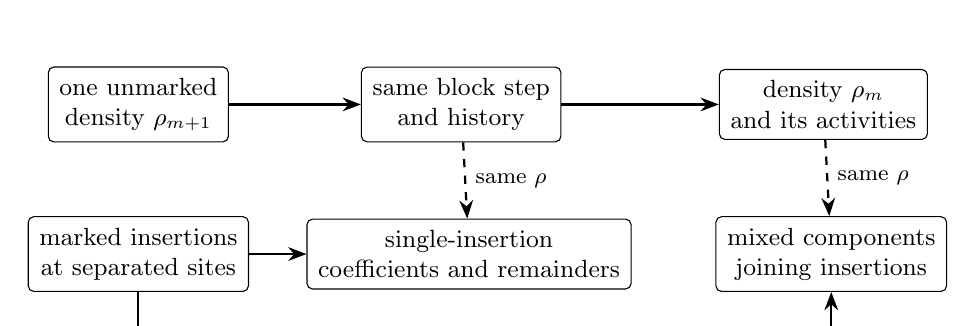
\begin{tikzpicture}[>=Stealth,font=\small,
  box/.style={draw,rounded corners=2pt,align=center,inner sep=4pt},
  ar/.style={->,thick}]
\node[box] (history) at (0,0) {one unmarked\\density $\rho_{m+1}$};
\node[box] (step) at (4.1,0) {same block step\\and history};
\node[box] (output) at (8.7,0) {density $\rho_m$\\and its activities};
\draw[ar] (history) -- (step); \draw[ar] (step) -- (output);
\node[box] (insertions) at (0,-1.9) {marked insertions\\at separated sites};
\node[box] (single) at (4.2,-1.9) {single-insertion\\coefficients and remainders};
\node[box] (mixed) at (8.8,-1.9) {mixed components\\joining insertions};
\draw[ar] (insertions) -- (single);
\draw[ar] (insertions.south) -- ++(0,-0.55) -| (mixed.south);
\draw[ar,dashed] (step) -- node[right,font=\footnotesize] {same $\rho$} (single);
\draw[ar,dashed] (output) -- node[right,font=\footnotesize] {same $\rho$} (mixed);
\end{tikzpicture}
\caption{Bookkeeping for marked insertions. The single-insertion decomposition has regular and forced remainders over the same unmarked density; components joining different insertions require their own estimates. Both tracks use the same underlying integration history.}\label{fig:rg-marked-tracks}
\end{figure}


\paragraph{Growing block ratios.}
The drift error of one step is bounded by a constant $\omega^{\rm RG}_j$ depending only on the stage $j=J_{m+1}$ (Theorem~\ref{prop:RG}). With a fixed block ratio~$\ell$, the accumulated drift bound $N\omega^{\rm RG}$ would be of the same order as the main term $\slope\log D_N=N\slope\log\ell$. The construction instead lets the ratios grow, $\log\ell_m\to\infty$ and $\log\ell_m/\log D_m\to0$, and chooses them with $\omega^{\rm RG}_j\le j^{-2}\log\ell_m$; the summed errors are then $o(\log D_m)$ and the exact one-loop slope survives (equation~\eqref{eq:I12-drift-sum}). Each level carries a stage $J_m$, with $4\le J_m\le J_{m+1}\le J_m+1$ and $J_m\to\infty$, which fixes the derivative order, the other estimate constants and the ratio $\ell_m=\ell^{\rm st}_{J_{m+1}}$. A stage may persist through many levels: entry into the next stage is delayed until the coupling and the period meet its requirements. Every fixed derivative order is therefore eventually available, while each step uses finitely many constants. All estimate constants of the induction are uniform in the volume; some are fixed before the block ratios and hence uniform in the ratio, the others may depend on a stage whose ratio is already fixed (Section~\ref{sec:constants}).

\subsection{Tuning, uniqueness and convergence}\label{sec:tuning-convergence}

Three different tasks concern the cutoff, and they are not interchangeable.
\begin{center}\small
\begin{tabular}{@{}p{0.27\textwidth}p{0.33\textwidth}p{0.33\textwidth}@{}}
\toprule
Task & Mechanism & What it does not supply\\
\midrule
Reach the endpoint coupling $\bar\beta$ at level zero & Continuous shooting and bracketing (Theorem~\ref{prop:MT}) & Uniqueness of the shooting parameter\\
Identify the limits at a fixed level & Weighted contraction toward the common endpoint (Proposition~\ref{prop:fixed-level}) & Convergence of the scalar normalizations\\
Remove the cutoff at fixed volume & Fixed-level convergence and a uniform stopping error (Theorem~\ref{prop:UV}) & An infinite-volume limit without refinement\\
\bottomrule
\end{tabular}
\end{center}
Uniqueness of the shooting parameter is not needed: trajectories for different cutoffs are compared only through their common endpoint, and two fixed-level limits with that endpoint coincide by the contraction. Remark~\ref{prop:endpoint-tuning} records the uniqueness and analytic dependence that the recursion also gives; the proofs do not use it.

\begin{figure}[ht]
\centering
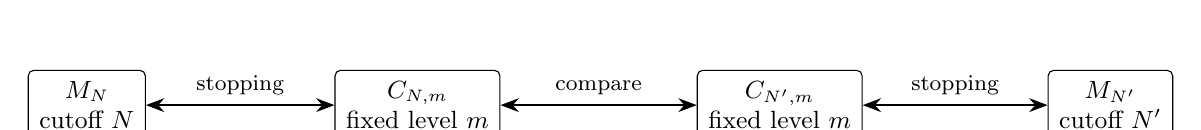
\begin{tikzpicture}[>=Stealth,font=\small,
  box/.style={draw,rounded corners=2pt,align=center,inner sep=4pt},
  ar/.style={->,thick}]
\node[box] (n) at (0,0) {$M_N$\\cutoff $N$};
\node[box] (cn) at (4.2,0) {$C_{N,m}$\\fixed level $m$};
\node[box] (cp) at (8.8,0) {$C_{N',m}$\\fixed level $m$};
\node[box] (np) at (13,0) {$M_{N'}$\\cutoff $N'$};
\draw[ar,<->] (n) -- node[above,font=\footnotesize] {stopping} (cn);
\draw[ar,<->] (cn) -- node[above,font=\footnotesize] {compare} (cp);
\draw[ar,<->] (cp) -- node[above,font=\footnotesize] {stopping} (np);
\end{tikzpicture}
\caption{At fixed volume index $p$, the ultraviolet comparison holds the intermediate level $m$ fixed while the cutoffs grow. Here $M_N$ is a lattice moment and $C_{N,m}$ its stopped level-$m$ comparison integral, defined below. The stopping and fixed-level bounds depend on the marked and graph estimates identified in the proof-status notice. Tuning gives the same endpoint coupling at level zero; it does not identify the full densities or their scalar normalizations.}\label{fig:rg-cutoff-comparison}
\end{figure}


The ultraviolet limit is a Cauchy argument through a common level (Figure~\ref{fig:rg-cutoff-comparison}). The stopping bound and the fixed-level marked graph comparison used below remain conditional on the higher-mode and graph estimates in \hyperref[par:proof-status]{the proof-status notice}. For insertions at points of $a_m\Z^4$, which lies in every finer lattice, let $M_N$ be the lattice moment and $C_{N,m}$ the normalized level-$m$ integral of the unmarked density and the transferred one-insertion functions, with the components joining two or more insertions omitted. For cutoffs beyond a threshold depending on~$m$,
\begin{align*}
|M_N-M_{N'}|&\le
\underbrace{|M_N-C_{N,m}|}_{\text{stopping error}}
+\underbrace{|C_{N,m}-C_{N',m}|}_{\text{fixed level}}
+\underbrace{|C_{N',m}-M_{N'}|}_{\text{stopping error}}\\
&\le4F_0e^{-B_m/64}+|C_{N,m}-C_{N',m}|,
\end{align*}
where $F_0$ does not depend on $m$ or on the cutoffs (Lemma~\ref{lem:E-stopping}). The reason is separation. At fine levels the sites of distinct insertions are at least $B_m^2$ apart, so every omitted component, which joins two or more insertions, has covering number at least $B_m/64$. Multiplying all these components by a complex~$z$ with $|z|<e^{B_m/64}$ therefore costs only two units of the support exponent, and the resulting normalized integral $F_m(z)$, carried back to a base level fixed before~$m$, is bounded there by~$F_0$. Since $F_m(1)=M_N$ and $F_m(0)=C_{N,m}$, Cauchy's estimate gives $|M_N-C_{N,m}|\le2F_0e^{-B_m/64}$. Choose $m$ to make the stopping errors small, hold it fixed, and let $N,N'\to\infty$. The middle term tends to zero for three reasons. First, the scalar normalization cancels. Write $\density^\circ\rho_{N,p,m}$ for the density of Definition~\ref{def:D06} with $v_{\rm sc}$ replaced by zero, so that $\density\rho_{N,p,m}=e^{v_{\rm sc}|\Lambda|}\density^\circ\rho_{N,p,m}$ with $\Lambda=\Lambda_{L_pD_m}$, and $H^\circ_{N,m}$ for the integrand of the numerator of $C_{N,m}$ with $v_{\rm sc}$ replaced by zero, formed from the same coordinates and the transferred one-insertion functions, regular and forced. Then
\begin{equation*}
C_{N,m}=\frac{\int e^{v_{\rm sc}|\Lambda|}H^\circ_{N,m}\,dU}{\int e^{v_{\rm sc}|\Lambda|}\density^\circ\rho_{N,p,m}\,dU}
=\frac{\int H^\circ_{N,m}\,dU}{\int\density^\circ\rho_{N,p,m}\,dU}\,,
\end{equation*}
and the constant $v_{\rm sc}$ of $\rho_{N,p,m}$, whose convergence is not asserted, drops out. Second, the unmarked coordinates converge at each fixed level (Proposition~\ref{prop:fixed-level}), and the denominator stays above a positive constant for all large cutoffs by restricting every link to a fixed small Haar-measure ball around the identity (Lemma~\ref{lem:E-fixed-level}). Third, the singleton functions converge by a common-core argument for the actual one-mark steps (Lemmas~\ref{lem:E-common-core} and~\ref{lem:E-fixed-level}). At each fixed level the steps contract distances by one half on a common complete class. If their outputs on each fixed input from a dense core converge, then, for any fixed $h>m$, the finite trajectories started from a common graph at level~$h$ converge at level~$m$. The selected trajectories differ from those auxiliary trajectories by at most $2^{1-(h-m)}$. First choose $h$ large, then the cutoffs. Convergence of the coefficient readout on the core, together with a uniform same-cutoff Lipschitz bound, transfers this comparison to the singleton functions. This argument still requires the common address dictionary, admissible truncations with their original eligibility tests, and convergence of the actual steps on the core, including their output tails. It does not supply the separate mixed- and higher-marker estimates used in the stopping bound. The bounds of Proposition~\ref{prop:UB} extend the resulting convergence from $\bigcup_ma_m\Z^4$ to all separated positions and to derivatives.

\subsection{Rotations}\label{sec:strategy-rotations}

Continuous rotational covariance is a conclusion of the construction; the hypercubic lattice symmetry does not supply it. The ultraviolet comparison identifies each $F_d$ with the Maxwell space through scaling frames (Propositions~\ref{prop:FC} and~\ref{prop:MC}). In degree four, divergence maps the centered real symmetric tensorial families onto the corresponding vectors of degree five with a one-dimensional kernel (Proposition~\ref{prop:conserved-line}), which supplies a conserved tensor~$J$. Its fluxes through small shells around one insertion define charge maps on the field spaces (Definition~\ref{def:D13}, Lemma~\ref{lem:G2.3}). Conservation turns the sum of the angular charges of all insertions into the integral of~$J$ against the derivative of a vector field that equals the rotation field $y\mapsto Ky$ on a large anisotropic box; the sum does not depend on the size of the box. For configurations on a coordinate axis through the origin this integral tends to zero by the coordinate reflection spaces of Definition~\ref{def:D14}, without a mass gap. The mechanism is a sign conflict (Lemmas~\ref{lem:H-coordinate-signs}, \ref{lem:H-G3} and~\ref{lem:G-collinear-flux}). Reflecting the integration variable in each axis replaces the spectator word by its projection that is odd under the reflections in the two axes of the rotation plane and even under the others. Because the word lies on a coordinate axis through the origin, the transverse reflections fix its positions, so this projection is again a combination of words on the axis. Such a combination has a positive spectral representation in each coordinate time axis, with the sign of its parity in that axis; one correlation represented with opposite signs bounds the low-energy spectral mass, and conservation with reflection positivity bounds that of the diagonal components of~$J$. Every term of the integral is then bounded by a negative power of the box size. Finite Ward tests identify the translation charges with derivatives; analyticity then extends the identity to all separated configurations; finite tests remove the defects in the rotation algebra, and the charges integrate to continuous representations of~$O(4)$ (Lemma~\ref{lem:G3.1}).

\subsection{Phases and reconstruction}\label{sec:strategy-reconstruction}

Reconstruction starts from separated Euclidean correlations and quantitative slab bounds; it does not require a positive extension across collision diagonals. Three objects should be kept apart.
\begin{center}\small
\begin{tabular}{@{}p{0.36\textwidth}p{0.57\textwidth}@{}}
\toprule
Object & Role\\
\midrule
$S_n^\xi$ on separated configurations & Euclidean correlations, reflection positive on positive-time words\\
Ordered-time continuations and boundary values & The Wightman functions and the relativistic fields\\
Contact extensions $\mathfrak D^\xi_{\boldsymbol A}$ & A specified extension through collisions, with controlled local order\\
\bottomrule
\end{tabular}
\end{center}
The infrared control available is a uniform low-energy estimate rather than a spectral gap. For a fixed finite combination $A$ of compactly supported smeared field words, uniformly in the phase~$\xi$,
\begin{align*}
\mu_{A\Omega_\xi}(\{0<\mathbf p^4\le u\})&\le M_Au^2&&(0<u\le1),\\
0\le\langle A\Omega_\xi,(e^{-sH_\xi}-P_{0,\xi})A\Omega_\xi\rangle&\le M'_As^{-2}&&(s\ge1),
\end{align*}
with $P_{0,\xi}$ the projection onto $\C\Omega_\xi$ (Lemma~\ref{lem:H2.3}). Vacuum uniqueness first holds for almost every phase; continuity of the vacuum-subtracted heat pairings in~$\xi$ and full support of~$\nu$ then extend it to every phase. The polynomial bound $M_Au^2$ is not a positive lower bound on the spectrum.

\subsection{The trace}\label{sec:strategy-trace}

The free Maxwell stress tensor is traceless, so a qualitative Maxwell limit cannot determine the first nonzero trace: it requires the next coefficient, with a rate. Heuristically, at scale~$r$ the rescaled trace $r^4\Theta$ is close, in the comparison maps, to $(4d_2/\beta(r))\curvaturesquare$, where $\curvaturesquare=\frac14\sum_{a,b,\alpha}{:}F^\alpha_{ab}F^\alpha_{ab}{:}$ is the free curvature square (Section~\ref{sec:trace-products}), with $d_2=-b_0/2$ and $\beta(r)\approx\slope\log(1/r)=2b_0\log(1/r)$, so that
\begin{equation*}
r^4\Theta\approx-\frac{\curvaturesquare}{\log(1/r)},\qquad
\tracetwopoint(r)\approx\frac{\maxwellcorr_2(\curvaturesquare,\curvaturesquare;-\tfrac r2e_4,\tfrac r2e_4)}{\log^2(1/r)}=\frac{3\dimG}{\pi^4}\,r^{-8}\log^{-2}(1/r)\,,
\end{equation*}
by homogeneity of degree $-8$. The amplitude does not depend on $b_0$: the trace coefficient and the running coupling both carry $b_0$, and only their ratio enters.

The coefficient $d_2$ is computed, not assumed, in five steps (Section~\ref{sec:partII-I}). (1)~The centered real symmetric $\hypercubic$-tensorial free tensors of degree four are spanned by the Maxwell stress, the trace direction $\delta_{ab}\curvaturesquare$ and one further tensor, and a linear functional reads the trace of such a tensor from its divergence. (2)~A lattice stress current built from plaquette curvatures has divergence equal to a variation of the action up to a small defect, and block transfer keeps its trace a lattice difference. (3)~This lattice Ward identity has the regulated coefficient $-12\slope$, the derivative $-\mu\,d/d\mu$ of a regulated one-loop determinant whose growth $12\slope\log\mu$ comes from the computation that gives the running slope (Lemmas~\ref{lem:C7} and~\ref{lem:I-regulator}). Along suitable radii the trace functional is carried to the continuum frames with error $o(E^{-1})$ for a slowly growing scale~$E$; the rate is needed because the cancelling coefficients of step~(4) may grow like a smaller scale~$R$, with $R/E\to0$ (Lemmas~\ref{lem:I-transfer} and~\ref{lem:I-stability}). (4)~Cancelling the divergence of the transferred current, multiplied by~$\beta$, with multiples of the other two tensors gives a conserved tensor. By Proposition~\ref{prop:conserved-line} it is a multiple of~$T$, the shell normalization forces the multiple to tend to one, and its coefficient along $\delta_{ab}\curvaturesquare$ tends to $d_2=-\slope/4$; the trace $4\curvaturesquare$ of that direction gives $4d_2/\beta$ (Proposition~\ref{prop:I-coefficient}). (5)~The positive spectral representation makes $\tracetwopoint$ nonincreasing, which turns this comparison along subsequences of radii into a limit through all radii (Section~\ref{sec:trace-products}). The product expansion, the last branch of Figure~\ref{fig:dependency}, is explained with its statement in Section~\ref{sec:trace-products}.


\section{The renormalization group}\label{sec:renormalization}

This section defines the block map, the coordinates of the effective densities and their norms, and states the inductive step, the multiscale theorem and the two ultraviolet results built on them. Fix $\blockpenalty>0$. Throughout we use the common choices of Sections~\ref{sec:partII-A}--\ref{sec:partII-E}, made once for the group realization and the penalty in the order of Section~\ref{sec:constants}; constants may depend on these choices, and further dependence is stated where it occurs.

\subsection{Scales and the block map}\label{sec:block-map}

With odd ratios $\ell_m\ge3$, set
\begin{equation}\label{eq:I12-levels}
D_0=1,\qquad D_{m+1}=\ell_mD_m,\qquad a_m=D_m^{-1},\qquad s_m=\log D_m\,.
\end{equation}
Level~$m$ has spacing~$a_m$, and blocking passes from level~$m+1$ to level~$m$; the level-$m$ torus has side $L_pD_m$ in lattice units and $L_p$ in physical units. The cutoff sequence of the family is $D_N$. Each level carries the stage $J_m$ of Section~\ref{sec:closes}. The endpoint coupling $\bar\beta>1$ is chosen large (item~7 of Table~\ref{tab:constant-choices}), and
\begin{align}\label{eq:I12-scales}
\refbeta_m&=\bar\beta+\slope s_m,&
\cutoffsize_m&=\exp\bigl((\log\log\refbeta_m)^2\bigr),&
t_m&=\refbeta_m^{-1/2}\cutoffsize_m,\\
B_m&=\lceil(\log\refbeta_m)^2\rceil,&
\epsilon_m^{\rm reg}&=\refbeta_m^{-11/10},&
\epsilon_m^{\rm for}&=e^{-(\cutoffsize_m)^{1/5}}\,.\label{eq:I12-scales-b}
\end{align}
The reference coupling $\refbeta_m$ follows the leading running slope; $t_m$ separates small from large plaquette fields; $B_m$ is the radius of the support weights; and $\epsilon_m^{\rm reg}$, $\epsilon_m^{\rm for}$ are the bounds kept by the induction for the regular and forced activity sums (Section~\ref{sec:closes} explains these sizes). They depend on the reference coupling, so they stay fixed as the actual coupling varies in the band $\mathfrak B_m=[\refbeta_m/2,2\refbeta_m]$. The physical periods $L_p$ are strictly increasing multiples of four, every positive integer divides $L_p$ for infinitely many~$p$, and $L_pD_m\ge100(B_m+1)$. At stage~$j$, $\mathfrak q_j$ is the derivative order, $\varpi_j$ the spatial power, $\sigma_j$ the support exponent and $\omega_j^{\rm RG}\ge0$ the coupling drift bound (Section~\ref{sec:constants}).

At a step $m+1\to m$, the fine links $U$ and coarse links $V$ live on $\Lambda_{L_pD_{m+1}}$ and $\Lambda_{L_pD_m}$; put $j=J_{m+1}$, $\ell=\ell_m$ and $\mathbb B_R=\{-R,\ldots,R\}^4$. Fine transports between two coarse endpoints are compared after expressing them in the same frames. A frame is a gauge transformation $h_{y,z}\in G$ at each fine site $\ell y+z$ of the patch of radius $(j+3)\ell$ around $\ell y$, built from parallel transports in the patch (Definitions~\ref{def:D20a}--\ref{def:D21}). For a coarse edge $e=(y,a)$ the framed straight connector is
\begin{equation}\label{eq:I12-framed-connector}
Y_{e,z}=h_{y,z}\left(\prod_{r=0}^{\ell-1}U(\ell y+z+re_a,a)\right)h_{y+e_a,z}^{-1}\,,
\end{equation}
the fine transport from $\ell y+z$ to $\ell(y+e_a)+z$ in the frames at its ends. With $\operatorname{Unif}$ the uniform probability on a box and $*j$ the $j$-fold convolution, the averaging weights and the predictor are
\begin{equation}\label{eq:I12-predictor}
\begin{gathered}
w_z^{\rm av}=\bigl(\operatorname{Unif}(\mathbb B_{(\ell-1)/2})\bigr)^{*j}(z),\qquad \overline Y_e=\sum_zw_z^{\rm av}Y_{e,z}\,,\\
Q_e^{\rm pred}=\operatorname*{argmin}_{u\in G}\sum_z w_z^{\rm av}\wilsonterm(Y_{e,z}u^{-1})=\operatorname*{argmin}_{u\in G}\|\overline Y_e-u\|_{\rm F}\,.
\end{gathered}
\end{equation}
The second form holds because $\wilsonterm(Yu^{-1})=(2n_G)^{-1}\|Y-u\|_{\rm F}^2$ for unitary $Y,u$: the predictor is the point of~$G$ nearest to the weighted average of the connectors, an average of group variables taken through the ambient matrices. On a good patch the connectors lie near one another, and this branch, on which the minimizer is unique, is used when the minimum lies below a fixed cutoff. Where the frame test or the predictor test fails, the kernel chooses at random, an axial frame from a finite list or a single connector $Y_{e,z}$ with probability $w^{\rm av}_z$; these branches complete the kernel on the remaining configurations (Section~\ref{sec:partII-B} gives the decision rules, summarized in Table~\ref{tab:B-branches} and Figure~\ref{fig:B-predictor}). A tag $\alpha_{\rm tag}$ records these discrete choices and nothing else: for each coarse site a frame label $(z,o)$, an offset $z\in\mathbb B_{(j+3)\ell}$ and an order~$o$ of the four axes, and for each coarse edge an offset $z\in\mathbb B_{(j+3)\ell}$ selecting a connector; on the minimizing branches the label is drawn uniformly and does not affect the kernel. Tags are drawn with probabilities
\begin{equation}\label{eq:I12-tag-mass}
\lambda^{\rm tag}(U,\alpha_{\rm tag})\ge0,\qquad
\sum_{\alpha_{\rm tag}}\lambda^{\rm tag}(U,\alpha_{\rm tag})=1\,.
\end{equation}
Given $U$ and the tag, the coarse links are independent, each concentrated within about $(\blockpenalty\beta)^{-1/2}$ of its predictor, with the normalized density $q_\gamma(u)=e^{-\gamma\wilsonterm(u)}/\int_Ge^{-\gamma\wilsonterm}\,dh$; the block penalty plays the role of the smearing parameter of soft block-spin transformations.

\begin{definition}[Exact block map]\label{def:D04}
For fine links $U$ and coarse links $V$, define
\begin{align*}
\blockkernel{m}_\beta(U,V)
&=\sum_{\alpha_{\rm tag}}\lambda^{\rm tag}(U,\alpha_{\rm tag})
\prod_{e\ {\rm coarse}}q_{\blockpenalty\beta}\bigl(V_eQ_e^{\rm pred}(U,\alpha_{\rm tag})^{-1}\bigr),\\
(\blockmap{m}_\beta f)(V)&=\int\blockkernel{m}_\beta(U,V)f(U)\,dU\,,
\end{align*}
with probability Haar measures on both link sets.
\end{definition}

For fixed $U$ and tag, right invariance of Haar measure makes each coarse factor integrate to one; summing the tag masses gives $\int\blockkernel{m}_\beta(U,V)\,dV=1$. Hence, for integrable~$f$,
\begin{equation}\label{eq:I12-partition-preservation}
\int(\blockmap{m}_\beta f)(V)\,dV=\int f(U)\,dU\,:
\end{equation}
the map integrates one scale exactly and keeps the partition integral. Branches, measurability and symmetries of the kernel are proved in Section~\ref{sec:partII-B}.

Probabilistically, a block step is the following experiment. Let $U$ have law $f(U)\,dU/\int f$ for an integrable $f\ge0$ with $\int f>0$; draw a tag with probabilities $\lambda^{\rm tag}(U,\cdot)$; and put $V_e=R_eQ_e^{\rm pred}(U,\alpha_{\rm tag})$, where the $R_e$ have density $q_{\blockpenalty\beta}$ and are independent of each other and of $(U,\alpha_{\rm tag})$. The pair $(U,V)$ then has law $f(U)\blockkernel{m}_\beta(U,V)\,dU\,dV/\int f$, and by Fubini the law of~$V$ has density $\blockmap{m}_\beta f/\int f$ with respect to Haar measure. Exactness refers to this identity, which includes every branch of the kernel. It does not mean that the coarse density is again a Wilson density; Section~\ref{sec:density} gives the coordinates in which it is written.

\subsection{The density and its norms}\label{sec:density}

The density produced by the integrations records four things: the leading curvature action with its running coupling, the field-independent scalar accumulated so far, small local corrections on small-field supports, and the contributions of large-field regions. At level~$m$ write $\Lambda=\Lambda_{L_pD_m}$. The flagged sites $\flags_m(U)$, or large-field sites, are the sites incident to a plaquette whose chord exceeds~$t_m$; a support is healthy, or small-field in the sense of Ba\l{}aban, if it contains none. Flags are gauge invariant, because plaquette chords are: the transform of the identity configuration in Section~\ref{sec:wilson} has no flagged site, however far its links are from the identity. A regular activity $E_i^{\rm reg}$ is a Borel real gauge-invariant function, local on its support $X_i$, anchored at $o_i\in X_i$ and vanishing at the flat configuration; it is used only on healthy supports. A forced activity $K_i^{\rm for}$, one of the large-field polymer activities, is local on its support $Y_i$ and carries a nonempty inventory $I_i\subset Y_i$ of flagged sites; it vanishes off its eligibility event
\begin{equation}\label{eq:I12-forced-eligibility}
\mathcal E_i^{\rm elig}=\{U:Y_i\cap\flags_m(U)=I_i\}\cap\mathcal E_i^{\rm extra},\qquad
K_i^{\rm for}(U)=0\quad(U\notin\mathcal E_i^{\rm elig})\,.
\end{equation}
The first condition fixes exactly which sites of $Y_i$ are flagged. The extra event is a fixed Borel gauge-invariant test supplied with the activity, which reads only links with both endpoints in $Y_i$ and the flags in~$Y_i$; it distinguishes local alternatives with the same support and inventory. The activity families are countable.

The path action carries the kinetic coefficient and the quadratic corrections generated by integration. At level~$m$ abbreviate the clipping constants and relaxation length of item~4 of Table~\ref{tab:constant-choices},
\begin{equation*}
c_{\rm dir}=c_{{\rm dir},J_m},\qquad c_{\rm lin}=c_{{\rm lin},J_m},\qquad 0<16c_{\rm lin}<c_{\rm dir}\le\min(\gamma_{J_m},1),\qquad R^{\rm rel}=R_{J_m}^{\rm rel}\,,
\end{equation*}
where $\gamma_j>0$ is half a uniform lower bound for the free effective plaquette forms of Lemma~\ref{lem:B2}. Distances are periodic maximum-coordinate distances in lattice units: on a torus of side~$n$, $\operatorname{dist}(x,y)=\min_{z\in n\Z^4}|\tilde x-\tilde y+z|_\infty$ for lifts $\tilde x,\tilde y\in\Z^4$. Set
\begin{align}\label{eq:I12-clipping}
\operatorname{clip}_{t}(r)&=
\begin{cases}c_{\rm dir}r^2/2,&r\le t,\\c_{\rm lin}tr,&r>t,\end{cases}\notag\\
\chi^{\rm rel}_{m,x}(U)&=\mathbf1\!\left\{
\chord(U_{y;ab})\le t_m e^{\operatorname{dist}(x,y)/R^{\rm rel}}
\text{ for every }y,a<b\right\}\,.
\end{align}
For each plaquette orientation $\mathfrak p=(a,b)$, let $\mathcal F_{\mathfrak p i}(U,x)$ be a curvature $\operatorname{proj}_{\g}(U_\square-U_\square^{-1})/2$, with the orthogonal projection for the metric of Definition~\ref{def:D01}, transported along a specified finite path to~$x$, and put $\mathcal L_{\mathfrak p}^{\rm path}(U,x)=\sum_i r_{\mathfrak p i}\mathcal F_{\mathfrak p i}(U,x)$, a smeared lattice curvature at~$x$. The action splits the effective kinetic form into a clipped part, quadratic below $t_m$ and linear beyond, and the remaining positive form, written as a sum of squares with one row per $(x,\mathfrak p)$; a row is switched off once some plaquette exceeds its distance-relaxed threshold, that is, when the \emph{relaxed threshold test} $\chi^{\rm rel}_{m,x}$ of~\eqref{eq:I12-clipping} vanishes. With $\mathfrak a_i^{(q)}(U,x)$, $q=2,3,4$, the fixed real invariant $q$-linear expressions in transported curvatures, each multiplied by the health indicator of its footprint (the union of its slot footprints and the anchor; Definition~\ref{def:D22}),
\begin{align}\label{eq:I12-path-action}
(\pathaction)^{\rm raw}_{N,m}(\beta,U)
&=\beta\sum_{x,\mathfrak p}\left[
\operatorname{clip}_{t_m}(\chord(U_{x;\mathfrak p}))
+\tfrac12\chi^{\rm rel}_{m,x}(U)|\mathcal L_{\mathfrak p}^{\rm path}(U,x)|^2\right]\notag\\
&\quad+\beta\sum_{x,i}(\mathfrak a_i^{(3)}+\mathfrak a_i^{(4)})(U,x)
+\sum_{x,i}\mathfrak a_i^{(2)}(U,x),\\
\pathaction_{N,m}(\beta,U)
&=|\hypercubic|^{-1}\sum_{h\in\hypercubic}(\pathaction)^{\rm raw}_{N,m}(\beta,h^*U)\,,\notag
\end{align}
where $h^*U$ transports links by the lattice isometry~$h$. The path coefficients and multilinear expressions are independent of~$p$ (Definitions~\ref{def:D22}--\ref{def:D23}, Lemmas~\ref{lem:C1}--\ref{lem:C2}); the action is affine in~$\beta$,
\begin{equation*}
\pathaction_{N,m}(\beta,U)=\beta\,\partial_\beta\pathaction_{N,m}(U)+\pathaction_{N,m}(0,U)\,,
\end{equation*}
where, after the average over~$\hypercubic$, $\partial_\beta\pathaction_{N,m}$ collects the clipped plaquette terms, the row squares with their switches $\chi^{\rm rel}_{m,x}$ and the cubic and quartic terms, and $\pathaction_{N,m}(0,\cdot)$ the quadratic terms~$\mathfrak a_i^{(2)}$. The clip drops at $r=t$ from $c_{\rm dir}t^2/2$ to $c_{\rm lin}t^2$. Accordingly the density coordinates are Borel functions; derivatives are taken only on healthy configurations with the masks held fixed, so coupling derivatives never differentiate the flag boundary. The positive linear branch beyond the threshold is what the local large-field energy bound (Lemma~\ref{lem:B-D1}) uses.

For these fixed path actions and thresholds, a \emph{representation} at level~$m$ is the datum
\begin{equation}\label{eq:I12-representation}
\rho=\bigl(\beta,v_{\rm sc},(X_i,o_i,E_i^{\rm reg})_i,
(Y_i,I_i,\mathcal E_i^{\rm extra},K_i^{\rm for})_i\bigr)\,,
\end{equation}
with scalar normalization per site $v_{\rm sc}$ (a constant in the effective density, not the vacuum vector of Section~\ref{sec:phases}) and running coupling $\beta(\rho)=\beta$. The running coupling is thus a coordinate fixed by the choice of path action: the coefficient of the fixed function $\partial_\beta\pathaction_{N,m}$, whose quadratic part is normalized so that $\beta$ is the coefficient of the squared curvature at zero momentum at every level, while the quadratic terms~$\mathfrak a_i^{(2)}$ carry no curvature-square term (Lemma~\ref{lem:C2}). It is not read off from the whole density, which also contains $v_{\rm sc}$ and the activities. Let $\mathfrak F_m(U)$ be the set of finite $\mathfrak a\subset\N$ such that the supports $Y_i$, $i\in\mathfrak a$, are pairwise disjoint and $\bigcup_{i\in\mathfrak a}I_i=\flags_m(U)$: the exact covers of the flagged sites.

\begin{definition}[Effective density]\label{def:D06}
For a representation~$\rho$, put
\begin{align*}
\mathcal V_\rho(U)&=\pathaction_{N,m}(\beta,U)+\sum_i\mathbf1_{X_i\,\mathrm{healthy}}E_i^{\rm reg}(U)-v_{\rm sc}|\Lambda|,\\
\density\rho(U)&=e^{-\mathcal V_\rho(U)}\sum_{\mathfrak a\in\mathfrak F_m(U)}\prod_{i\in\mathfrak a}K_i^{\rm for}(U)\,.
\end{align*}
\end{definition}

If there are no flagged sites, $\mathfrak F_m(U)=\{\varnothing\}$ and the forced sum is one. Otherwise every flagged site lies in exactly one selected support, but the sum runs over all exact covers: one support may carry two flags in one term while two disjoint supports carry one flag each in another (Figure~\ref{fig:covers}). The local regularity of the activities and the restrictions on forced terms are Definitions~\ref{def:D24}--\ref{def:D25}.

\begin{figure}[ht]
\centering
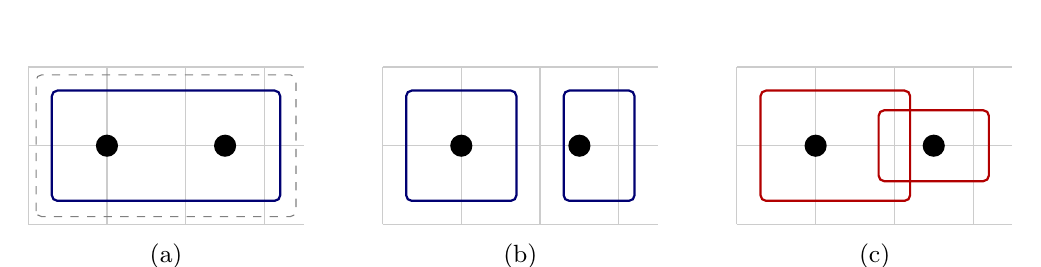
\begin{tikzpicture}[x=0.5cm,y=0.5cm,font=\small]
\foreach \dx/\lab in {0/(a),9/(b),18/(c)}{
 \begin{scope}[shift={(\dx,0)}]
 \draw[gray!40] (0,0) grid (7,4);
 \node at (3.5,-0.8) {\lab};
 \end{scope}}
\draw[thick,paperlink,rounded corners=2pt] (0.6,0.6) rectangle (6.4,3.4);
\draw[dashed,gray,rounded corners=2pt] (0.2,0.2) rectangle (6.8,3.8);
\draw[thick,paperlink,rounded corners=2pt] (9.6,0.6) rectangle (12.4,3.4);
\draw[thick,paperlink,rounded corners=2pt] (13.6,0.6) rectangle (15.4,3.4);
\draw[thick,red!70!black,rounded corners=2pt] (18.6,0.6) rectangle (22.4,3.4);
\draw[thick,red!70!black,rounded corners=2pt] (21.6,1.1) rectangle (24.4,2.9);
\foreach \dx in {0,9,18}{\fill (\dx+2,2) circle (4pt); \fill (\dx+5,2) circle (4pt);}
\end{tikzpicture}
\caption{Exact covers of two flagged sites (dots). (a) One support carries both flags; the dashed line marks the larger region its eligibility test inspects. (b) Two disjoint supports carry one flag each. Both selections occur in the sum of Definition~\ref{def:D06}, which does not choose a canonical cover. (c) Overlapping supports are not a cover.}\label{fig:covers}
\end{figure}

For a link $e$ let $e^-$ be its initial site. The left derivative $D^L_{\dot{\mathcal A}}$ differentiates the increments $U_e\mapsto e^{t\dot{\mathcal A}_e}U_e$, with $\dot{\mathcal A}_e\in\g$ normed by Definition~\ref{def:D01}.

\begin{definition}[Local derivative seminorm]\label{def:D05a}
For a regular activity anchored at $o_i$, set
\begin{equation*}
\|E_i^{\rm reg}\|_m=
\sup_{0\le q\le\mathfrak q_{J_m}}\ \sup_{U,\dot{\mathcal A}_1,\ldots,\dot{\mathcal A}_q}
\bigl|D^L_{\dot{\mathcal A}_1}\cdots D^L_{\dot{\mathcal A}_q}E_i^{\rm reg}(U)\bigr|\,,
\end{equation*}
over configurations healthy on $X_i$ and directions with $|(\dot{\mathcal A}_k)_e|\le t_m\bigl(1+\operatorname{dist}(e^-,o_i)\bigr)^{\varpi_{J_m}}$, $1\le k\le q$.
\end{definition}

The seminorm measures ordered local derivatives in units of the permitted field size. For a support~$X$, let $\cover_{B_m}(X)$ be the least number of radius-$B_m$ lattice balls with connected union covering~$X$; the exponential weight below penalizes supports that need many such balls.

\begin{definition}[Weighted activity sums]\label{def:D05b}
For nonnegative majorants $e_i^{\rm maj}\ge\|E_i^{\rm reg}\|_m$ and $k_i^{\rm maj}\ge\sup_U|K_i^{\rm for}(U)|$, define
\begin{equation*}
\mathcal E_m=\sup_x\sum_{o_i=x}e^{\sigma_{J_m}\cover_{B_m}(X_i)}e_i^{\rm maj},\qquad
\mathcal K_m=\sup_x\sum_{x\in Y_i}e^{\sigma_{J_m}\cover_{B_m}(Y_i)}k_i^{\rm maj}\,.
\end{equation*}
\end{definition}

The two sums are formed differently (Figure~\ref{fig:weighted-sums}). The regular sum at~$x$ counts the activities anchored at~$x$, whatever their supports, so each regular activity is counted once, at the site from which its derivative directions are weighted (Definition~\ref{def:D05a}). The forced sum at~$x$ counts every forced activity whose support contains~$x$, so the weight $e^{\sigma_{J_m}\cover_{B_m}(Y_i)}$ charges a large support at each of its sites; if $x$ is flagged, every activity that covers~$x$ in a term of Definition~\ref{def:D06} is counted there. Section~\ref{sec:partII-D} converts anchored bounds into containing-site bounds where needed, at the cost of the number of possible anchors of a support.

\begin{figure}[ht]
\centering
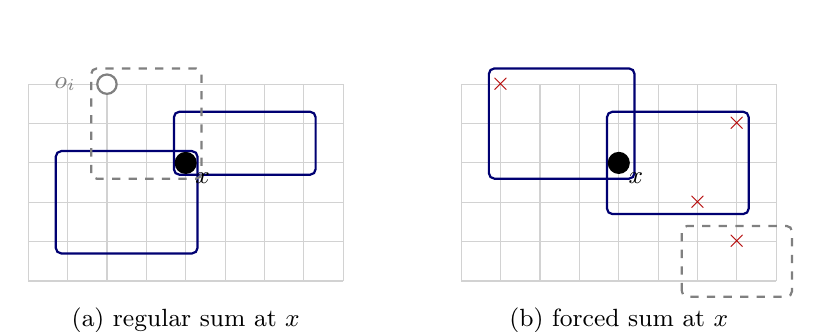
\begin{tikzpicture}[x=0.5cm,y=0.5cm,font=\small]
\foreach \dx/\lab in {0/{(a) regular sum at $x$},11/{(b) forced sum at $x$}}{
 \begin{scope}[shift={(\dx,0)}]
 \draw[gray!35,step=1] (0,0) grid (8,5);
 \node at (4,-1) {\lab};
 \end{scope}}
\draw[thick,paperlink,rounded corners=2pt] (3.7,2.7) rectangle (7.3,4.3);
\draw[thick,paperlink,rounded corners=2pt] (0.7,0.7) rectangle (4.3,3.3);
\draw[thick,dashed,gray,rounded corners=2pt] (1.6,2.6) rectangle (4.4,5.4);
\draw[thick,gray,fill=white] (2,5) circle (3.5pt);
\node[gray,left=2pt] at (1.6,5) {$o_i$};
\draw[thick,paperlink,rounded corners=2pt] (14.7,1.7) rectangle (18.3,4.3);
\draw[thick,paperlink,rounded corners=2pt] (11.7,2.6) rectangle (15.4,5.4);
\draw[thick,dashed,gray,rounded corners=2pt] (16.6,-0.4) rectangle (19.4,1.4);
\foreach \p in {(17,2),(18,4),(12,5),(18,1)}{\node[red!70!black] at \p {$\times$};}
\foreach \dx in {0,11}{\fill (\dx+4,3) circle (4pt); \node[below right=0pt] at (\dx+4,3) {$x$};}
\end{tikzpicture}
\caption{The weighted sums of Definition~\ref{def:D05b} at a site~$x$. (a) The regular sum counts the activities anchored at~$x$ (solid supports), whatever their extent; the dashed support contains~$x$ but is anchored at $o_i\ne x$ and is counted at~$o_i$. (b) The forced sum counts every activity whose support contains~$x$ (solid), whatever its inventory (crosses); overlapping supports both count, since the sum runs over activities, not covers. The dashed support does not contain~$x$.}\label{fig:weighted-sums}
\end{figure}

The induction keeps the bounds
\begin{equation}\label{eq:I12-activity-caps}
\mathcal E_m\le\epsilon_m^{\rm reg},\qquad \mathcal K_m\le\epsilon_m^{\rm for}\,.
\end{equation}
These numerical bounds do not by themselves define the classes on which the step acts. The Wilson start is the continuous curve
\begin{equation}\label{eq:I12-Wilson-initialization}
\beta\longmapsto\rho^{\rm W}_\beta,\qquad
\beta(\rho^{\rm W}_\beta)=\beta,\qquad
\density\rho^{\rm W}_\beta=e^{-\beta E^{\rm W}_{L_pD_N}}
\quad(\beta\in\mathfrak B_N)\,,
\end{equation}
with scalar normalization zero (Lemma~\ref{lem:D3}). The \emph{admissible classes} consist of everything reachable from it. Let $\mathcal I_{N,p}=\{\rho^{\rm W}_\beta:\beta\in\mathfrak B_N\}$ and $\mathcal A_{N,N,p}=\mathcal I_{N,p}$. For $m<N$, a representation at level~$m$ belongs to $\mathcal A_{N,m,p}$ if it is obtained from some $\rho'\in\mathcal A_{N,m+1,p}$ with coupling in~$\mathfrak B_{m+1}$ by one block step of Section~\ref{sec:partII-D}: its path is $\pathaction_{N,m}$, its activities are produced by local subtraction, path replacement and fusion, its coupling is that of~$\rho'$ plus the one-loop coefficient $\alpha_{N,m}$ of Lemma~\ref{lem:C7} and a correction bounded by the first inequality of~\eqref{eq:D-retained}, and its density is the block integral of the density of~$\rho'$ (the precise conditions precede Lemma~\ref{lem:D2}). Membership is a property of a single representation; in particular the classes contain the outputs of the step construction on continuous curves and their restrictions to closed subintervals. Let $\mathcal R_{N,m,p}\subset\mathcal A_{N,m,p}\times\mathcal A_{N,m+1,p}$ be the set of the corresponding output--input pairs. Every member satisfies Definitions~\ref{def:D24}--\ref{def:D25}, the path bounds of Lemmas~\ref{lem:C1}--\ref{lem:C2} and~\eqref{eq:I12-activity-caps} (Lemma~\ref{lem:D3} at the Wilson start, Lemmas~\ref{lem:D1} and~\ref{lem:D2} at later levels). A curve $u\mapsto\rho_u$ in $\mathcal A_{N,m,p}$ is continuous (Definition~\ref{def:D25a}) if its supports, anchors, inventories and extra tests do not depend on~$u$, its coupling and scalar normalization are continuous, and, as $u\to u_0$, the differences of regular derivatives on healthy configurations and of forced values in supremum norm admit majorants whose weighted sums tend to zero.

\subsection{The inductive step}\label{sec:inductive-step}

Exact integration removes one scale. Extracting its marginal curvature-square term into the coupling leaves a bounded drift error and returns a density in the next admissible class.

\begin{theorem}[RG. One step]\label{prop:RG}
For every $N,p$, $m<N$, reals $u_0\le u_1$ and continuous $\rho'_u\in\mathcal A_{N,m+1,p}$ with $\beta'_u=\beta(\rho'_u)\in\mathfrak B_{m+1}$ for all $u\in[u_0,u_1]$, there is a continuous $\rho_u\in\mathcal A_{N,m,p}$ with $(\rho_u,\rho'_u)\in\mathcal R_{N,m,p}$ and, for every $u\in[u_0,u_1]$ and coarse configuration $V$,
\begin{align*}
\density\rho_u(V)&=(\blockmap{m}_{\beta'_u}\density\rho'_u)(V),\\
\beta(\rho_u)&=\beta'_u-\slope\log\ell_m+e_u,
\qquad |e_u|\le\omega_{J_{m+1}}^{\rm RG}\,.
\end{align*}
\end{theorem}

\emph{Idea of the proof} (Sections~\ref{sec:partII-B}--\ref{sec:partII-D}; the proof follows Lemma~\ref{lem:D2}).
\begin{enumerate}[label=\textup{Step \arabic*.},leftmargin=4.2em,nosep]
\item The density identity is exact because the output coordinates rewrite the block-integrated density on every configuration (Lemma~\ref{lem:D5}); by~\eqref{eq:I12-partition-preservation} the partition integral is kept. Approximation enters only the coupling drift and the activity estimates.
\item On small fields, gauge fixing in a rooted block-tree gauge and the stationary background turn the local integral into a Gaussian integral with its determinant and Haar-coordinate factors; the large-field lower bound (Lemma~\ref{lem:B-D1}) supplies suppression of the forced terms.
\item Classical fourth-order matching fixes the local terms, and the background curvature-square coefficient of the one-loop action, assembled from the inherited quadratic loop term, the fluctuation determinant and the Haar Jacobian, gives the change $-\slope\log\ell_m$ up to a stage-bounded error (Lemma~\ref{lem:C7}).
\item The local expansion, the contraction of inherited terms and the five-torus localization (Lemma~\ref{lem:five-torus}) give the regular bound; forced fusion gives the forced bound; the scalar coupling reset absorbs the residual kinetic coefficient (Lemma~\ref{lem:C8}).
\end{enumerate}
The bound $\omega_j^{\rm RG}$ depends only on the stage, not on $N,p$, the interval or the curve. Since $\refbeta_m=\refbeta_{m+1}-\slope\log\ell_m$, a step changes $\beta-\refbeta$ by $e_u$ only.

\subsection{Multiscale trajectories}\label{sec:trajectories}

A trajectory is a tuple $\rho_{N,p,m}\in\mathcal A_{N,m,p}$, $0\le m\le N$, with $\rho_{N,p,N}\in\mathcal I_{N,p}$ and $(\rho_{N,p,m},\rho_{N,p,m+1})\in\mathcal R_{N,m,p}$ for $m<N$; write $\beta_{N,p,m}=\beta(\rho_{N,p,m})$. The bare coupling is selected by shooting. Put $\mathfrak T_m=[\bar\beta+\tfrac{\slope}2s_m,\ \bar\beta+2\slope s_m]\subset\mathfrak B_m$, so that $\mathfrak T_0=\{\bar\beta\}$. Start with the Wilson curve on $\mathfrak T_N$. Suppose a closed parameter interval has level-$(m+1)$ couplings in $\mathfrak T_{m+1}$, taking its end values at its endpoints. Since $s_{m+1}=s_m+\log\ell_m$ and $|e_u|\le\omega^{\rm RG}_{J_{m+1}}\le\tfrac{\slope}4\log\ell_m$ (item~5 of Table~\ref{tab:constant-choices}), the output couplings at the two endpoints satisfy
\begin{equation*}
\beta\le\bar\beta+\tfrac{\slope}2s_m-\tfrac{\slope}4\log\ell_m<\min\mathfrak T_m,\qquad
\beta\ge\bar\beta+2\slope s_m+\tfrac{3\slope}4\log\ell_m>\max\mathfrak T_m\,.
\end{equation*}
The intermediate value theorem gives a closed subinterval whose couplings lie in $\mathfrak T_m$ and take its end values at its endpoints. After $N$ steps the level-zero coupling is $\bar\beta$. The couplings are chosen this way for all $N,p$ before any sequence of volume indices is prescribed. Trajectories for different cutoffs thus share the coupling~$\bar\beta$ at level zero; their scalar normalizations and activities need not agree (Figure~\ref{fig:two-cutoffs}), and Proposition~\ref{prop:fixed-level} below compares them at a fixed level as the cutoff grows.

\begin{figure}[ht]
\centering
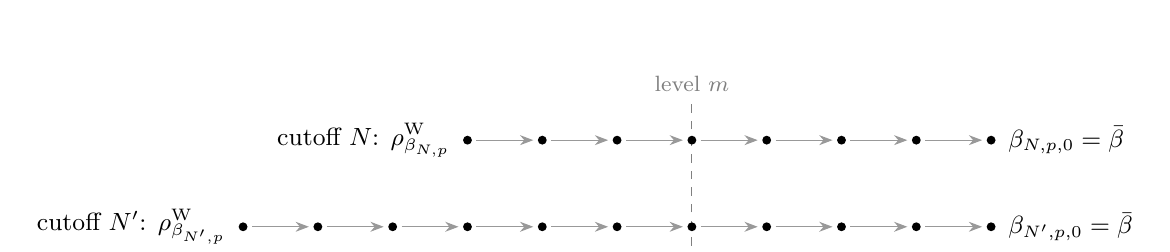
\begin{tikzpicture}[x=0.95cm,y=1cm,>=Stealth,font=\small]
\draw[dashed,gray] (6,-0.45) -- (6,1.6) node[above,font=\footnotesize] {level $m$};
\foreach \i in {0,...,9}{\draw[->,gray!80] (\i+0.12,0) -- (\i+0.88,0);}
\foreach \i in {3,...,9}{\draw[->,gray!80] (\i+0.12,1.1) -- (\i+0.88,1.1);}
\foreach \i in {0,...,10}{\fill (\i,0) circle (1.6pt);}
\foreach \i in {3,...,10}{\fill (\i,1.1) circle (1.6pt);}
\node[left] at (2.9,1.1) {cutoff $N$: $\rho^{\rm W}_{\beta_{N,p}}$};
\node[left] at (-0.1,0) {cutoff $N'$: $\rho^{\rm W}_{\beta_{N',p}}$};
\node[right] at (10.1,1.1) {$\beta_{N,p,0}=\bar\beta$};
\node[right] at (10.1,0) {$\beta_{N',p,0}=\bar\beta$};
\end{tikzpicture}
\caption{Trajectories for two cutoffs $N<N'$ at one volume, from the Wilson start at the cutoff (left) to level zero (right); each arrow is a block step, and levels are aligned vertically. Both reach the coupling~$\bar\beta$ at level zero; their scalar normalizations and activities need not agree. At a fixed level~$m$ (dashed), Proposition~\ref{prop:fixed-level} states convergence of the couplings and activities as the cutoff tends to infinity, subject to cutoff continuity in the activity norms and convergence of the path drift.}\label{fig:two-cutoffs}
\end{figure}

\begin{theorem}[MT. Multiscale trajectory]\label{prop:MT}
There are bare couplings $\beta_{N,p}$ and trajectories $(\rho_{N,p,m})_{m=0}^N$, for all $N,p\in\N$, with $\rho_{N,p,N}=\rho^{\rm W}_{\beta_{N,p}}$ and $\beta_{N,p,N}=\beta_{N,p}$, satisfying
\begin{gather*}
\beta_{N,p,0}=\bar\beta,\qquad \beta_{N,p,m}\in\mathfrak B_m\quad(0\le m\le N),\\
\density\rho_{N,p,m}=\blockmap{m}_{\beta_{N,p,m+1}}\density\rho_{N,p,m+1}\quad(m<N)\,.
\end{gather*}
For every $\varepsilon>0$, some $m_0(\varepsilon)$ satisfies
\begin{equation*}
|\beta_{N,p,m}-\slope s_m|\le\varepsilon s_m
\qquad(N\ge m\ge m_0,\ p\in\N)\,.
\end{equation*}
\end{theorem}

The proof is the shooting argument above (Section~\ref{sec:partII-E.1}, Lemmas~\ref{lem:E1.1}--\ref{lem:E1.2}). Fix these trajectories for all later constructions. The drift bound of Theorem~\ref{prop:RG} holds on every adjacent pair, and all their integrals equal $Z_{L_pD_N,\beta_{N,p}}$ by~\eqref{eq:I12-partition-preservation} and the Wilson start. Summing the drift from the fixed endpoint gives
\begin{equation}\label{eq:I12-drift-sum}
|\beta_{N,p,m}-\refbeta_m|\le\sum_{i=0}^{m-1}\omega_{J_{i+1}}^{\rm RG}\,.
\end{equation}
Item~5 of Table~\ref{tab:constant-choices} bounds the sum by $(\slope/4)s_m$, which also keeps the couplings in $\mathfrak B_m$. Its stronger bound $\omega_{J_{i+1}}^{\rm RG}\le J_{i+1}^{-2}\log\ell_i$ makes the sum $o(s_m)$: split it at a fixed level and bound the tail by $\sup_{i\ge i_0}J_{i+1}^{-2}$ times~$s_m$. Since $J_i\to\infty$ and $s_m\to\infty$, the finite initial sum and $\bar\beta$ disappear after division by~$s_m$, uniformly in $N\ge m$ and~$p$. As $\omega_j^{\rm RG}\ge1$, the same bound forces $\log\ell_m\ge J_{m+1}^2\to\infty$: the block ratios must grow, and the level choices also give $\log\ell_m/s_m\to0$. The step construction of Theorem~\ref{prop:RG} is fixed once on whole continuous curves (Lemma~\ref{lem:D2}); the trajectories it produces from $\rho^{\rm W}_\beta$, and their restrictions, form the \emph{specified recursion}, to which the trajectories of Theorem~\ref{prop:MT} belong. Different cutoffs are compared through the following limit.

\begin{proposition}[Fixed-level convergence]\label{prop:fixed-level}
For fixed $p$ and $m$, as $N\to\infty$ along the full sequence, the couplings $\beta_{N,p,m}$ of
Theorem~\ref{prop:MT} converge, and the activity coordinates of $\rho_{N,p,m}$ converge in the
weighted spaces $\mathcal X_{m,p}$ of~\eqref{eq:D-common-norm}. No convergence of the scalar normalizations is asserted.
\end{proposition}

\emph{Idea of the proof} (Lemmas~\ref{lem:D-cutoff-continuity} and~\ref{lem:D-fixed-level}). The truncated-coordinate comparison and uniqueness argument require cutoff continuity in the full activity norms and convergence of the path drift; those inputs remain open. The argument uses geometric truncation, not compactness of a ball in an infinite-dimensional space. The running-coupling coordinates lie in fixed compact intervals, so a diagonal argument gives subsequential limits. At a fixed higher level $k$, replace the activity coordinate by zero and run the same maps down to level~$m$: the error is at most $(8g_*)^{k-m}$ with $g_*=1/128$, uniformly in the cutoff, while the truncated coordinates converge by the cutoff compatibility of finitely many step maps (Lemma~\ref{lem:D-cutoff-continuity}). Letting $k\to\infty$ gives the activity limits. Two limits have the same endpoint $\bar\beta$, and their distance $\mathfrak d_\infty$ satisfies $\mathfrak d_\infty\le8g_*\mathfrak d_\infty$, so they coincide.

\subsection{Local fields under blocking}\label{sec:marked}

Blocking a density that carries one insertion returns a density of the same form: the unmarked density times a local insertion with new coefficients, plus regular remainders with vanishing Taylor coefficients through order~$d$ and forced remainders attached to large fields. The coefficients evolve linearly, and the insertions of Definition~\ref{def:D08} are normalized by prescribing them at the reference level. Choose the reference level $\reflevel{d}$ with $J_{\reflevel{d}}\ge d+3$ and $\mathfrak q_{J_m}\ge d+1$, $\varpi_{J_m}\ge d$ for $m\ge\reflevel{d}$ (Lemma~\ref{lem:E2.1}). Fix $N\ge\reflevel{d}$; starting from a fine-cutoff coefficient vector $\mathbf v\in V_d$, the marked density at the origin is initialized and blocked by
\begin{align}\label{eq:I12-marked-evolution}
H^{\rm ins}_{N,p,N;d}(\mathbf v;U)
&=\density\rho_{N,p,N}(U)\,
\localsection{d}[t_N^{-\factorcount}\mathbf v](0;U),\\
H^{\rm ins}_{N,p,m;d}(\mathbf v)
&=\ell_m^d\blockmap{m}_{\beta_{N,p,m+1}}
H^{\rm ins}_{N,p,m+1;d}(\mathbf v)
\quad(\reflevel{d}\le m<N)\,.
\end{align}
For fixed $N,p,d$, the transfer construction chooses coefficient vectors $\mathbf x_m(\mathbf v)$ and regular and forced remainders $R_{m,i}^{\rm reg}(\mathbf v)$, $Q_{m,i}^{\rm for}(\mathbf v)$, all linear in~$\mathbf v$. Write $\mathbf x_m=x_{m,0}\mathbf1+\mathbf x_m^\circ$ and $\rho_m=\rho_{N,p,m}$. The regular remainders have supports $Z_{m,i}$ containing the origin. Their sum and the forced remainder are
\begin{align}\label{eq:I12-marked-remainders}
\mathcal R_m^{\rm reg}(\mathbf v;U)
&=\sum_i\mathbf1_{Z_{m,i}\,\mathrm{healthy}}R_{m,i}^{\rm reg}(\mathbf v;U),\notag\\
\mathcal R_m^{\rm for}(\mathbf v;U)
&=e^{-\mathcal V_{\rho_m}(U)}\sum_{\mathfrak a\in\mathfrak F_m(U)}\sum_{i\in\mathfrak a}
Q_{m,i}^{\rm for}(\mathbf v;U)\prod_{j\in\mathfrak a\setminus\{i\}}K_j^{\rm for}(U)\,,
\end{align}
with all unmarked quantities taken from~$\rho_m$. The marked density has the exact decomposition
\begin{multline}\label{eq:I12-marked-representation}
H^{\rm ins}_{N,p,m;d}(\mathbf v;U)=\density\rho_m(U)\left[
x_{m,0}(\mathbf v)+\mathbf1_{\Sigma_d\,\mathrm{healthy}}
\localsection{d}[t_m^{-\factorcount}\mathbf x_m^\circ(\mathbf v)](0;U)\right]\\
+\density\rho_m(U)\mathcal R_m^{\rm reg}(\mathbf v;U)
+\mathcal R_m^{\rm for}(\mathbf v;U)\,,
\end{multline}
with the stencil $\Sigma_d$ placed at the origin of the level-$m$ torus. If $10\operatorname{dist}(x,0)<L_pD_m$ for every $x\in Z_{m,i}$, the regular remainder $R_{m,i}^{\rm reg}$ has zero radial-jet Taylor coefficients through order~$d$; the forced remainders vanish outside their unmarked eligibility events (Lemmas~\ref{lem:E2.2}--\ref{lem:E2.2a}). The fixed decomposition selected there gives the terminal map of Definition~\ref{def:D08}, invertible by Lemma~\ref{lem:E2.1}:
\begin{equation*}
\mathbf x_N(\mathbf v)=\mathbf v,\qquad
\mathbf x_{\reflevel{d}}(\mathbf v)=\mathsf Z_{N,p,d}\mathbf v\,.
\end{equation*}
The factor $\ell_m^d=(a_m/a_{m+1})^d$ uses the degree of the whole space $V_d$, and the terminal map accounts for the mixing between its weights. The unit identity $\mathbf x_m(a_N^d\mathbf1)=a_m^d\mathbf1$, proved with the transfer symmetries (Lemma~\ref{lem:E2.1a}), explains why the coefficient of the constant insertion is $a_{\reflevel{d}}^d\mathbf1$, although $V_d$ also contains polynomials of lower weight. With Theorem~\ref{prop:MT}, these insertions specify one Wilson family; each insertion is continuous, gauge invariant and local on its fixed stencil, and Theorem~\ref{prop:MT} at $m=N$ gives the volume-uniform slope $\slope>0$.

\subsection{Uniform bounds and the fixed-volume limit}\label{sec:uv-limit}

For a finite list $\boldsymbol l$ of pairs $(i,a)$, with $i$ a slot and $a$ an axis, the normalized differences and derivatives are
\begin{equation*}
\Delta_{\boldsymbol l}=\prod_{(i,a)\in\boldsymbol l}a_N^{-1}(\tau_{i,a}-1),\qquad
\partial_{\boldsymbol l}=\prod_{(i,a)\in\boldsymbol l}\partial_{x_i^a}\,,
\end{equation*}
where $\tau_{i,a}$ shifts slot~$i$ forward by one lattice link. The torus separation of a lattice tuple is $\min_{i\ne j}\min_{z\in L_p\Z^4}|\hat y_i-\hat y_j+z|_\infty$, with value $+\infty$ for $n\le1$, and
\begin{equation*}
\Gen{n}=\{x:x_i^a\ne x_j^a\text{ for }i\ne j,\ a=1,\ldots,4\},\qquad
\NoHit{L}{n}=\{x:x_i-x_j\notin L\Z^4\text{ for }i\ne j\}\,;
\end{equation*}
the last set excludes collisions on a torus of physical side~$L$. The first result bounds lattice correlations and their differences independently of the volume.

\begin{proposition}[UB. Uniform difference bounds]\label{prop:UB}
For every $v\in\mathcal T^n$, finite difference list~$\boldsymbol l$ and $r>0$, there are $B(v,\boldsymbol l,r)\ge0$ and $N_0(v,\boldsymbol l,r)$ such that, for every $N\ge N_0$, every~$p$ and every lattice tuple of torus separation at least~$r$,
\begin{equation*}
|\Delta_{\boldsymbol l}\latmoment_{N,p}(v;y)|\le B\,.
\end{equation*}
\end{proposition}

\emph{Idea of the proof} (Section~\ref{sec:partII-E.2}). Choose an intermediate level whose physical blocks fit below the separation, so the insertions lie in distinct blocks. By the decomposition~\eqref{eq:I12-marked-representation}, at that level each insertion is a bounded local function plus small remainders, with bounds independent of $N$ and~$p$; differences of insertions are matched in a higher degree, their equation directions are removed, and the remaining coefficients are tested against a finite free comparison matrix, whose injectivity (Lemma~\ref{lem:E2-free-tests}) rests on the free positivity of Lemma~\ref{lem:G1.1}. The chessboard estimate then bounds the correlation by a product of reflected moments, schematically
\begin{equation*}
\Bigl|\Bigl\langle\prod_iO_i\Bigr\rangle\Bigr|\le\prod_i\Bigl\langle\prod_{g\in\mathcal G}gO_i\Bigr\rangle^{1/|\mathcal G|}
\end{equation*}
for $O_i$ localized in distinct blocks and $\mathcal G$ generated by the reflections in the block boundaries; each factor is independent of the volume. The reflected-moment constant is chosen before the intermediate level, and only the cutoff threshold depends on it.

The second result removes the spacing at each fixed volume along the full sequence; Section~\ref{sec:tuning-convergence} displays the Cauchy argument.

\begin{theorem}[UV. Fixed-volume limit]\label{prop:UV}\label{thm:UV}
For every $p,n$ and $v\in\mathcal T^n$, there is $M^{\rm UV}_{p,v}\in C^\infty(\NoHit{L_p}{n})$ such that, for every finite~$\boldsymbol l$ and every $p$-admissible separated test~$f$,
\begin{equation*}
\lim_{N\to\infty}a_N^{4n}\sum_{y\in\Lambda_{L_pD_N}^n}f(\hat y)\Delta_{\boldsymbol l}\latmoment_{N,p}(v;y)
=\int f(x)\partial_{\boldsymbol l}M^{\rm UV}_{p,v}(x)\,dx\,.
\end{equation*}
\end{theorem}

\emph{Idea of the proof} (Lemmas~\ref{lem:E3.1}--\ref{lem:E3.2}). The Cauchy argument of Section~\ref{sec:tuning-convergence} gives convergence on $\bigcup_ma_m\Z^4$: the transferred correlations at a fixed level converge, and the stopping error $2F_0e^{-B_m/64}$, with $F_0$ independent of~$m$, compares them with the original ones. Proposition~\ref{prop:UB} extends convergence to all separated positions and identifies every derivative, also at moving points crossing the boundary of the chosen period cell.
For $\boldsymbol l=\varnothing$ the left side is $\lim_N\latsmear_{N,p}(v;f)$, so the inner limits of Definition~\ref{def:D09} exist at every admissible volume; admissibility places the support of~$f$ inside $\NoHit{L_p}{n}$. The limiting kernel is periodic in each position and smooth away from periodic collisions, including where positions share coordinates. The thresholds may depend on~$p$.

\section{The continuum limit, stress, phases, trace and products}\label{sec:continuum-results}

The lattice family of Section~\ref{sec:renormalization} is now fixed; its couplings and insertions were chosen before any sequence of volume indices. This section takes the volume limit and identifies the continuum fields: their calculus, the stress tensor and the rotations, the phases and their reconstruction, the trace law and the products. Constants may depend on the group, its realization, the penalty and the construction choices of Section~\ref{sec:constants}; further dependence is stated.

\subsection{The volume limit and the field calculus}\label{sec:volume-limit}

One volume refinement serves every field and all later constructions.
\nopagebreak
\begin{theorem}[IV. Infinite-volume limit]\label{prop:IV}\label{thm:IV}
For every strictly increasing $\mathsf p:\N\to\N$, there are a strictly increasing $\mathsf q:\N\to\N$ and a multilinear table~$S$ such that the Wilson family converges to~$S$ along $P=\mathsf p\circ\mathsf q$ in the sense of Definition~\ref{def:D09}. The table satisfies E1--E7.
\end{theorem}
\begin{remark}[Dependence on the volume sequence]\label{rem:volume-choice}
The limiting table~$S$ may depend on the prescribed sequence~$\mathsf p$ and the refinement~$\mathsf q$, hence on the retained volume indices~$P=\mathsf p\circ\mathsf q$.
\end{remark}
Fix~$\mathsf p$, $\mathsf q$, $P$ and~$S$ from now on.

\emph{Idea of the proof} (Lemmas~\ref{lem:F1}--\ref{lem:F3}).
\begin{enumerate}[label=\textup{Step \arabic*.},leftmargin=4.2em,nosep]
\item Proposition~\ref{prop:UB} bounds the correlations and all their lattice differences uniformly in the volume; a diagonal extraction along~$\mathsf p$ gives local smooth limits on~$\Conf{n}$ (E6). At each admissible volume the fixed-volume kernels are those of Theorem~\ref{prop:UV}, so the full inner limit is kept; only the outer limit uses a subsequence.
\item The chessboard seminorm, the cost of repeating one observation throughout the box, gives~\ref{it:E7} at order zero, and the corrected derivative maps below give it at positive orders; lattice reflection positivity passes to the limit, giving~\ref{it:E5} and then~\ref{it:E4}.
\item A further refinement fixes finitely many coefficient maps in each degree. This auxiliary subsequence concerns finite-dimensional coefficients only; the limits of the correlations are the full ultraviolet limits already established.
\end{enumerate}

The coefficient maps are needed because the normalization $a_N^{-d}\mathsf Z_{N,p,d}^{-1}$ depends on the degree. The same $c\in V_d\subset V_e$ defines different lattice fields as $(d,c)$ and as $(e,c)$, and a lattice difference of a degree-$d$ insertion is a degree-$(d+1)$ object with yet another normalization; the naive inclusion $V_d\to V_e$ does not preserve correlations. Lemma~\ref{lem:F2} constructs linear \emph{corrected coefficient maps} relating these normalizations, and they induce the inclusions and derivatives of the next proposition. Its dimension statement uses a Gaussian comparison theory, introduced by its covariance.

\begin{definition}[Free Maxwell comparison]\label{def:D11}
For $\dimG$ independent colours, let $A_a^\alpha$ be centred generalized Gaussian fields on~$\R^4$ with
\begin{equation*}
\mathbb E A_a^\alpha(x)A_b^\beta(y)
=\delta_{\alpha\beta}\delta_{ab}\Gamma(x-y),\qquad
\Gamma(x)=\frac1{4\pi^2|x|^2},\qquad F_{ab}=\partial_aA_b-\partial_bA_a\,,
\end{equation*}
the derivatives taken in the sense of distributions. Let $\maxwellspace{d}$ consist of the complex $\operatorname{Ad}(G)$-invariant Wick polynomials in curvature jets of weight at most~$d$, modulo antisymmetry, the linear Bianchi identities and $\sum_a\partial_aF_{ab}=0$. Their separated Wick correlations are~$\maxwellcorr$.
\end{definition}

Each component of~$A$ is a massless free field, with covariance $(-\Delta)^{-1}$ since $-\Delta\Gamma=\delta_0$, and $F$ is the free Maxwell field. Wick polynomials in curvature jets at distinct points have smooth correlations, computed by Wick's theorem from derivatives of~$\Gamma$ at nonzero arguments. The relations are of two kinds. Antisymmetry and the Bianchi identities $\partial_aF_{bc}+\partial_bF_{ca}+\partial_cF_{ab}=0$ hold identically, since $F$ is a derivative of~$A$. The equation $\sum_a\partial_aF_{ab}=0$ holds only in separated correlations: by $-\Delta\Gamma=\delta_0$,
\begin{equation*}
\mathbb E\Bigl(\sum_a\partial_aF^\alpha_{ab}\Bigr)(x)\,F^\beta_{cd}(y)=\delta_{\alpha\beta}\bigl(\delta_{bd}\partial_{x^c}-\delta_{bc}\partial_{x^d}\bigr)\delta_0(x-y)\,,
\end{equation*}
which vanishes for $x\ne y$, so every separated Wick correlation with a factor of the divergence vanishes; but the divergence is not the zero distribution, since its covariance is $\delta_{\alpha\beta}(\partial_b\partial_d-\delta_{bd}\Delta)\delta_0(x-y)$. The quotient by this equation thus records a relation among separated correlations, not an identity of distributions. The comparison of Proposition~\ref{prop:MC} likewise concerns separated correlations at short distances; it does not identify the constructed fields with this Gaussian reference.

The constant one is the Maxwell unit, coefficient conjugation gives the real structure, and inclusions keep the same polynomial at a larger weight bound. Free differentiation is $\partial_a^{\rm Max}(:P:)=:\partial_aP:$, and the rotation action $R_d^{\rm Max}(h)(:P:)=:hP:$ is determined by $hF_{ab}^\alpha=\sum_{i,j}h_{ia}h_{jb}F_{ij}^\alpha$ and $h\partial_a=\sum_ih_{ia}\partial_ih$ for $h\in O(4)$; these operations preserve the defining relations.

\begin{proposition}[FC. Field calculus]\label{prop:FC}
For the table~$S$ of Theorem~\ref{prop:IV}, there are complex linear maps $\jmath_{d,e}:F_d\to F_e$ for $d\le e$ and $\partial_a:F_d\to F_{d+1}$ for every $d,a$ such that, for every $A\in F_d$,
\begin{gather*}
\iota_e\circ\jmath_{d,e}=\iota_d,\qquad
\iota_{d+1}(\partial_aA)=\partial_{x_0^a}\iota_d(A),\\
\dim_\C F_d=\dim_\C\maxwellspace{d}\,.
\end{gather*}
\end{proposition}

The proof is Lemma~\ref{lem:F2}. The corrected coefficient maps supply representatives of inclusions and derivatives; the equation and rank comparisons of Lemmas~\ref{lem:E2.6}--\ref{lem:E2.10} bound $\dim F_d$ from above, and the free tests of Lemma~\ref{lem:E2-free-tests}, with the free positivity of Lemma~\ref{lem:G1.1}, bound it from below. Each $\iota_d$ is injective by Definition~\ref{def:D10}, so the inclusions are unique and injective, $\jmath_{e,f}\jmath_{d,e}=\jmath_{d,f}$, $\jmath_{d,d}=\mathrm{id}$, and by~\ref{it:E1} they carry $\unitfield{d}$ to~$\unitfield{e}$. Their images are nested, so $\mathcal L=\bigcup_d\iota_dF_d$. Permutation symmetry gives, for $\boldsymbol A\in\prod_iF_{d_i}$, $x\in\Conf{n}$, slot~$i$ and axis~$a$,
\begin{equation*}
\partial_{x_i^a}S_n(\boldsymbol A;x)=S_n(A_1,\ldots,\partial_aA_i,\ldots,A_n;x)\,,
\end{equation*}
and~\ref{it:E2} with injectivity of the responses makes inclusions and derivatives commute with conjugation, inclusions commute with~$\hypercubic$, and $h\partial_a=\sum_bh_{ba}\partial_bh$ for $h\in\hypercubic$.

The table also defines reflection Hilbert spaces along the coordinate axes. They and their slab bounds use only the volume limit and the field calculus (Lemmas~\ref{lem:F3}, \ref{lem:F4} and Proposition~\ref{prop:FC}), and they enter the rotation argument of Section~\ref{sec:stress} before continuous rotations are available.

\begin{definition}[Coordinate reflection spaces]\label{def:D14}
For an axis~$a$, let $\mathcal H_a^{\rm OS}$ be the completion of the complex span of words at distinct points in $\{x^a>0\}$ modulo the null space of $\langle w,v\rangle_a=S(\theta_a(w)\,v)$, and put $e^{-tH_a^{\rm OS}}[v]=[\tau_{te_a}v]$ for $t\ge0$. Let $\Omega_a^{\rm OS}$ be the class of the empty word and $P^0_a$ the projection onto $\ker H_a^{\rm OS}$.
\end{definition}

By~\ref{it:E4} the form is positive semidefinite; with~\ref{it:E7}, the translations $\tau_{te_a}$, $t\ge0$, preserve its null space and define a strongly continuous self-adjoint contraction semigroup, whose generator is $H_a^{\rm OS}\ge0$ (proof of Lemma~\ref{lem:H1.1}). Inserting a word between positive-time vectors is bounded after a positive time translation (Lemma~\ref{lem:H1.1}); these slab bounds are the coordinate estimates used before rotations.

\subsection{Stress and rotations}\label{sec:stress}

The fields are compared with Maxwell fields at small distances, through bases that may vary with the radius to accommodate mixing, and a conserved tensor is then normalized by its shell fluxes. The volume refinement and~$S$ remain fixed; the subsequences below concern comparison radii only.

\begin{definition}[Scaling frames]\label{def:D12}
A scaling sequence consists of $r_k>0$, $r_k\to0$, and complex linear isomorphisms $\scaleframe{k}{d}:\maxwellspace{d}\to F_d$. It is stable if, for every $D\in\N$, these maps eventually preserve conjugation, $\hypercubic$, units and inclusions exactly in all degrees $d\le e\le D$. Scaling dimensions are included in the maps: a comparison insertion is $\scaleframe{k}{d}u$ at~$r_kx$, with no further factor~$r_k^d$.
\end{definition}

After rescaling positions the interacting correlations approach their Maxwell counterparts; one sequence serves every fixed list of fields.

\begin{proposition}[MC. Maxwell comparison]\label{prop:MC}
There is one stable scaling sequence such that, for every arity~$n$, degree list $(d_i)$ and $u_i\in\maxwellspace{d_i}$,
\begin{equation*}
S_n(\scaleframe{k}{d_i}u_i;r_k\,\cdot\,)\longrightarrow\maxwellcorr_n(u;\cdot)
\quad\text{in }L^1_{\rm loc}(\Conf{n})\,.
\end{equation*}
\end{proposition}

\emph{Idea of the proof} (Lemma~\ref{lem:G2.1}). The lattice comparison stops near the requested physical scale and compares the correlations with the free Gaussian ones. Finitely many separating correlations make the comparison maps injective, the upper bound $\dim_\C F_d\le\dim_\C\maxwellspace{d}$ of Proposition~\ref{prop:FC} makes them isomorphisms, and finite-dimensional corrections impose the eventual equalities. Local $L^1$ convergence is equivalent, by duality and smooth approximation on slightly larger separated compact sets, to convergence uniform over smooth tests with $\|f\|_\infty\le1$ and fixed compact support. This weaker form is used to construct and normalize the conserved current, before the stress tensor exists.

To read translation and angular charge, integrate a conserved symmetric tensor through a shell surrounding one insertion. In a free model the shell integral can be computed, and it differentiates the enclosed correlation. Let $\phi$ be a massless free scalar field with covariance~$\Gamma$, write $\langle\cdot\rangle$ for its Wick correlations, and put $T^\phi_{ab}=-{:}\partial_a\phi\,\partial_b\phi{:}+\frac12\delta_{ab}{:}|\nabla\phi|^2{:}$, the negative of the canonical tensor. With $\Gamma_0=\Gamma(y-x_0)$ and $\Gamma_1=\Gamma(y-x)$,
\begin{equation*}
\langle T^\phi_{ab}(y)\phi(x_0)\phi(x)\rangle=-\partial_a\Gamma_0\,\partial_b\Gamma_1-\partial_b\Gamma_0\,\partial_a\Gamma_1+\delta_{ab}\nabla\Gamma_0\cdot\nabla\Gamma_1\,,
\end{equation*}
whose divergence in~$y$ vanishes away from $x_0$ and~$x$, where $\Delta\Gamma_0=\Delta\Gamma_1=0$. Take a smooth compactly supported $\chi$ equal to one on the ball of radius $\epsilon<|x-x_0|$ about~$x_0$ and vanishing near~$x$. The divergence theorem turns the flux $-\sum_a\int\partial_a\chi(y)\langle T^\phi_{ab}(y)\phi(x_0)\phi(x)\rangle\,dy$ into the integral of $\sum_a\langle T^\phi_{ab}(y)\phi(x_0)\phi(x)\rangle n_a$ over the boundary sphere of that ball, with outer normal~$n$. There $\nabla\Gamma_0=-n/(2\pi^2\epsilon^3)$, the last two terms cancel, and the integrand is $\partial_b\Gamma_1/(2\pi^2\epsilon^3)$. The sphere has area $2\pi^2\epsilon^3$ and $\partial_b\Gamma(\cdot-x)$ is harmonic on the ball, so the mean value property gives the flux $\partial_b\Gamma(x_0-x)=\partial_{x_0^b}\langle\phi(x_0)\phi(x)\rangle$. This free calculation illustrates the identity that Theorem~\ref{prop:ST} establishes for the constructed fields by a different route.

We normalize the stress tensor in the same way, so that its translation flux acts as $+\partial_{x_0^b}$ on the enclosed insertion; with the minus sign in the flux below, this gives the negative of the usual Euclidean canonical Maxwell tensor (displayed after Theorem~\ref{prop:ST}). Let $A\in F_d$, let $\boldsymbol B$ be a list of~$n$ spectator fields at~$x$, and take $(x_0,x)\in\Conf{n+1}$.

\begin{definition}[Shell fluxes]\label{def:D13}
For $J_{ab}=J_{ba}\in F_4$ with $\sum_a\partial_aJ_{ab}=0$ and $K_{\rm rot}\in\mathfrak{so}(4)$, choose a real shell cutoff $\chi\in C_c^\infty(\R^4)$ equal to one near~$x_0$ and supported away from the spectators. Define
\begin{align*}
\mathcal P_b^J&=-\sum_a\int\partial_a\chi(y)
S(J_{ab}(y),A(x_0),\boldsymbol B(x))\,dy,\\
\mathcal Y_{K_{\rm rot}}^J&=-\sum_{a,b}\int\partial_a\chi(y)(K_{\rm rot}(y-x_0))_b
S(J_{ab}(y),A(x_0),\boldsymbol B(x))\,dy\,.
\end{align*}
\end{definition}

The integrals avoid every insertion point, and they do not depend on the shell cutoff: two choices differ by a function vanishing near every insertion, integration by parts with Proposition~\ref{prop:FC} removes the divergence term, and the extra angular term is $\sum_{a,b}(K_{\rm rot})_{ba}J_{ab}=0$ since $K_{\rm rot}$ is skew and $J$ symmetric. Conservation makes the flux independent of the radius of the shell; it does not by itself control a flux through a distant surface. A field is real when fixed by conjugation; a family $J_{ab}\in F_4$ is $\hypercubic$-tensorial when $hJ_{ab}=\sum_{i,j}h_{ia}h_{jb}J_{ij}$ for $h\in\hypercubic$, conserved when $\sum_a\partial_aJ_{ab}=0$ in~$F_5$ for every~$b$, and centered when every component has zero one-point function.

\begin{proposition}[Conserved line]\label{prop:conserved-line}
The centered real symmetric $\hypercubic$-tensorial conserved families $(J_{ab})$ in~$F_4$ form a real vector space of dimension one.
\end{proposition}

This is the first assertion of Lemma~\ref{lem:G2.2}; its proof shows that divergence maps the centered real symmetric tensorial families onto the corresponding vectors in degree five, with one-dimensional kernel. Along a refinement of the sequence of Proposition~\ref{prop:MC}, positive multiples of the rescaled nonzero member approach the free stress line in the degree-four frames. For a nonzero member~$J$, Lemma~\ref{lem:G2.3} constructs complex linear charge maps $\mathsf p_b:F_d\to F_{d+1}$ and $\mathsf Y_{K_{\rm rot}}:F_d\to F_d$, the latter real linear in~$K_{\rm rot}$, with $\mathcal P_b^J=S((\mathsf p_bA)(x_0),\boldsymbol B(x))$ and $\mathcal Y_{K_{\rm rot}}^J=S((\mathsf Y_{K_{\rm rot}}A)(x_0),\boldsymbol B(x))$ for every degree, field, spectator list, separated configuration and shell cutoff.

These charges restore the rotations. Conservation of~$J$ turns the sum of the angular charges of the insertions, each combining $\mathsf Y_{K_{\rm rot}}$ at its own point with the translation charge weighted by the rotated position, into the integral of~$J$ against the derivative of a vector field equal to $y\mapsto K_{\rm rot}y$ on a large anisotropic box. For configurations on a coordinate axis through the origin, the coordinate reflection spaces of Definition~\ref{def:D14} show that this integral tends to zero as the box grows (Lemma~\ref{lem:G-collinear-flux}; Section~\ref{sec:strategy-rotations} explains the mechanism), so the angular sum vanishes there. Finite Ward tests then identify $\mathsf p_b$ with $c_\star\partial_b$, and analyticity extends the identity, infinitesimal rotation invariance, to all separated configurations. Lemma~\ref{lem:G3.1} thereby constructs continuous complex linear representations $R_d$ of~$O(4)$, extending~$\hypercubic$, fixing units and commuting with conjugation and inclusions; for a real $c_\star\ne0$ common to every degree,
\begin{equation*}
\mathsf L_d(K_{\rm rot})=\left.\frac{d}{dt}R_d(e^{tK_{\rm rot}})\right|_{t=0},
\qquad \mathsf p_b=c_\star\partial_b,\qquad
\mathsf Y_{K_{\rm rot}}=c_\star\mathsf L_d(K_{\rm rot})\,.
\end{equation*}
Integrating gives full covariance (Lemma~\ref{lem:G3.1}): $S_n(R_{d_i}(h)A_i;hx)=S_n(\boldsymbol A;x)$ for every $\boldsymbol A\in\prod_iF_{d_i}$, $x\in\Conf{n}$ and $h\in O(4)$. A family is $O(4)$-tensorial if $R_4(h)J_{ab}=\sum_{i,j}h_{ia}h_{jb}J_{ij}$ for every $h\in O(4)$. The common constant~$c_\star$ fixes the normalization of the stress tensor by its action on fields.

\begin{theorem}[ST. Stress tensor]\label{prop:ST}\label{thm:ST}
There is a real symmetric $O(4)$-tensorial family $T_{ab}\in F_4$ with $\sum_a\partial_aT_{ab}=0$ such that, for every degree, field, spectator list, separated configuration and shell cutoff of Definition~\ref{def:D13}, every~$b$ and every $K_{\rm rot}\in\mathfrak{so}(4)$,
\begin{equation*}
\mathcal P_b^T=\partial_{x_0^b}S(A(x_0),\boldsymbol B(x)),\qquad
\mathcal Y_{K_{\rm rot}}^T=S((\mathsf L_d(K_{\rm rot})A)(x_0),\boldsymbol B(x))\,.
\end{equation*}
\end{theorem}

The proof is in Lemmas~\ref{lem:G3.1}--\ref{lem:G3.2}: divide $J$ by~$c_\star$ and average its tensor transform over~$O(4)$ with probability Haar measure. Covariance and the transformation laws of derivatives and generators give the same shell Ward identities for each transformed current, and integration preserves them, as well as symmetry, reality, centering and conservation. Fix this tensor; it is centered, since $J$ is and $R_4$ preserves zero one-point values. The free stress $\maxwellstress$ is normalized by the same shell Ward identities, with $\partial_a^{\rm Max}$ and the free generators $\mathsf L_d^{\rm Max}$ (Section~\ref{sec:partII-G.1}):
\begin{equation*}
\maxwellstress_{ab}=-\sum_{c,\alpha}:F_{ac}^\alpha F_{bc}^\alpha:
+\frac{\delta_{ab}}4\sum_{i,j,\alpha}:F_{ij}^\alpha F_{ij}^\alpha:\,.
\end{equation*}

The last comparison includes stress insertions. For a free list $u_1,\ldots,u_n$, $u_i\in\maxwellspace{d_i}$, a stress-slot choice is a subset $I\subset\{1,\ldots,n\}$ with component pairs $(a_i,b_i)$ for $i\in I$; put $A_i^0=\maxwellstress_{a_ib_i}$ for $i\in I$ and $A_i^0=u_i$ otherwise. The shell Ward identities fix the stress normalization, so its comparison insertion needs only the engineering factor~$r_k^4$. Below, $D_x^j$ differentiates the whole function $x\mapsto S_n(\boldsymbol A_k;r_kx)$.

\begin{proposition}[SC. Differentiated short-distance comparison]\label{prop:SC}
Along the refinement of the scaling sequence of Proposition~\ref{prop:MC} chosen in Lemma~\ref{lem:G2.2}, for every fixed free list and stress-slot choice, every derivative order~$j$ and compact $\mathcal K\subset\Conf{n}$, with $A_{k,i}=r_k^4T_{a_ib_i}$ on~$I$ for the fixed tensor of Theorem~\ref{prop:ST} and $A_{k,i}=\scaleframe{k}{d_i}u_i$ elsewhere,
\begin{equation*}
D_x^jS_n(\boldsymbol A_k;r_kx)\longrightarrow D_x^j\maxwellcorr_n(\boldsymbol A^0;x)
\quad\text{uniformly on }\mathcal K\,.
\end{equation*}
\end{proposition}
Fix this refined sequence $(r_k,\scaleframe{k}{d})$ from now on. The proof follows Lemma~\ref{lem:G3.3}; with $I=\varnothing$ and $j=0$ it gives Proposition~\ref{prop:MC} in uniform form, but the earlier comparison is needed first, to construct the tensor. Along this sequence, for fixed $d,a,K_{\rm rot}$, the transported infinitesimal actions converge in operator norm: $r_k(\scaleframe{k}{d+1})^{-1}\partial_a\scaleframe{k}{d}\to\partial_a^{\rm Max}$ and $(\scaleframe{k}{d})^{-1}\mathsf L_d(K_{\rm rot})\scaleframe{k}{d}\to\mathsf L_d^{\rm Max}(K_{\rm rot})$.

\subsection{Phases and reconstruction}\label{sec:phases}

Compression to zero energy separates the mixed correlations into phases. In the reflection space of the time axis, a long empty time interval removes the positive-energy components; the word insertions that survive commute on the zero-energy space, and a character of the algebra they generate assigns compatible scalar values to all of them. The phases are these characters. We now use the fourth coordinate as time.

\begin{definition}[Compression]\label{def:compression}
For $h_{\rm sl}>0$ and a word $w$ with times in $(0,h_{\rm sl})$, let $\mathsf B_{h_{\rm sl}}(w)$ be the bounded extension to $\mathcal H_4^{\rm OS}$ (Lemma~\ref{lem:H1.1}) of the slab insertion $A_wv=w\,\tau_{h_{\rm sl}e_4}v$ on positive-time words~$v$, and put $M^0(w)=P^0_4\mathsf B_{h_{\rm sl}}(w)|_{\ker H_4^{\rm OS}}$.
\end{definition}

The slab insertion places $w$ in the slab $(0,h_{\rm sl})$ below the translated state. A separated word is translated into a slab to define its compression; Lemma~\ref{lem:H1.2} proves independence of width and placement and that the compressed operators generate a separable commutative unital C$^*$-algebra
\begin{equation*}
\mathfrak A_0=C^*(M^0(w):w\text{ separated})
\end{equation*}
with cyclic and separating vector $\Omega_4^{\rm OS}$. Its vacuum state $a\mapsto\langle\Omega_4^{\rm OS},a\Omega_4^{\rm OS}\rangle$ satisfies $S(w)=\langle\Omega_4^{\rm OS},M^0(w)\Omega_4^{\rm OS}\rangle$ by translation invariance; the measure below represents this state on the character space, and the separating property gives full support. Call a character $\xi$ a phase and $S^\xi$ its table.

\begin{theorem}[PH. Phase decomposition]\label{prop:PH}
The algebra $\mathfrak A_0$ has a compact metric character space $\phases$ with a full-support probability measure $\nu$ such that, for every separated word $w$,
\begin{equation*}
S^\xi(w)=\xi(M^0(w)),\qquad S(w)=\int_{\phases}S^\xi(w)\,d\nu(\xi)\,.
\end{equation*}
Each phase satisfies E1--E7 and has exactly the null spaces $\nullspace{d}(S^\xi)=\nullspace{d}(S)$. The identities of FC, $O(4)$ covariance and ST hold with $S^\xi$ in place of $S$, for the same maps and tensor $T$. For fixed $w$, $\xi\mapsto S^\xi(w)$ is continuous.
\end{theorem}

\emph{Idea of the proof} (Lemmas~\ref{lem:H1.1}, \ref{lem:H1.2} and~\ref{lem:H1.3}). The matrix element $\langle[u],M^0(w_1)M^0(w_2)[v]\rangle$ is a limit of correlations of four words placed far apart in time; the long time intervals project onto $\ker H_4^{\rm OS}$. The same four words can instead be spread along a second positive coordinate direction, so that the two middle words occur in the opposite order. By $O(4)$ covariance (Lemma~\ref{lem:G3.1}) both arrangements have the same limit, so $M^0(w_1)M^0(w_2)=M^0(w_2)M^0(w_1)$: rotation covariance is an input to the phase decomposition. Reflection positivity holds in each phase because the compressed reflected Gram matrices are positive operators and characters are positive; that no field becomes null in a phase uses the free tests at short distances. Commutativity alone gives neither.

For each phase apply Definitions~\ref{def:D14} and~\ref{def:compression} to $S^\xi$, obtaining $\mathcal H_{4,\xi}^{\rm OS}$, $H_{4,\xi}^{\rm OS}$ and $\Omega_\xi^{\rm OS}$. Fix $\xi_*$ in the full-measure set with one-dimensional time-axis reflection ground space supplied by Lemma~\ref{lem:H1.3}; Theorem~\ref{prop:RC} extends ground-space uniqueness to every phase. Two further notions enter the reconstruction and the trace law.

\begin{definition}[Bounded weak commutant]\label{def:D14d}
A bounded operator $B$ belongs to the weak commutant if, for every smeared field $\Phi$ and all $u,v\in\mathcal D$, one has $u\in\operatorname{Dom}\Phi^*$ (automatic by~\ref{def:W1}) and $\langle\Phi^*u,Bv\rangle=\langle u,B\Phi v\rangle$, where $\Phi^*$ is the Hilbert-space adjoint.
\end{definition}

\begin{definition}[Hermitian scalar labels]\label{def:D14e}
A label is Hermitian if $\ell^*=\ell$, and Lorentz scalar if $\rho_{\rm lab}(\Lambda,0)\ell=\ell$ for every $\Lambda\in SO^+(1,3)$.
\end{definition}

For the theory at a phase $\xi$ write $\mathcal H_\xi$, $\mathcal D_\xi$, $\Omega_\xi$, $\Phi_\xi$, $\mathsf T_\xi$, and define its energy by $\mathsf T_\xi(te_4)=e^{itH_\xi}$. Its reflection comparison map is the linear isometry $\mathsf J_\xi^{\rm OS}:\mathcal H_\xi\to\mathcal H_{4,\xi}^{\rm OS}$ with $\mathsf J_\xi^{\rm OS}\Omega_\xi=\Omega_\xi^{\rm OS}$ that sends each product of smeared fields applied to the vacuum to the norm limit of its heat-regularized positive-time reflection vectors as the ordered heights tend to zero (proofs of Lemmas~\ref{lem:H2.1} and~\ref{lem:H2.2}).

\begin{theorem}[RC. Reconstruction]\label{prop:RC}
For every $\xi\in\phases$, there are a faithful Wightman theory (Definition~\ref{def:wightman}) on $\mathcal L$ and functions $\mathsf F_n^\xi$ satisfying Definitions~\ref{def:D15} and~\ref{def:D14f} with the response maps $\iota_d$ of Definition~\ref{def:D10}. Its OS comparison map $\mathsf J_\xi^{\rm OS}$ is unitary, intertwines spatial translations and satisfies $\mathsf J_\xi^{\rm OS}e^{-sH_\xi}=e^{-sH_{4,\xi}^{\rm OS}}\mathsf J_\xi^{\rm OS}$ for $s\ge0$, and
\begin{equation*}
\ker H_\xi=\C\Omega_\xi,\qquad \ker H_{4,\xi}^{\rm OS}=\C\Omega_\xi^{\rm OS}\,.
\end{equation*}
Every bounded operator in the weak commutant of its fields is scalar.
\end{theorem}

\emph{Idea of the proof} (Lemmas~\ref{lem:H2.1}--\ref{lem:H2.4}). Reflection positivity supplies the Hilbert spaces and the nonnegative energy; the slab bounds supply the growth estimates behind the boundary values; the restored rotations, continued to boosts, supply Lorentz covariance and, with the continuation, locality. The uniform low-energy estimate of Section~\ref{sec:strategy-reconstruction}, continuity of the vacuum-subtracted heat pairings and full support of~$\nu$ extend vacuum uniqueness from almost every phase to every phase, so the choice of~$\xi_*$ stays valid. The same lemmas give joint Schwartz distributions, phase averages and stress continuation.

The label maps are common to all phases. The adjoint is induced by time reflection followed by conjugation, $(\iota_dA)^*=\iota_d(R_d(\mathsf s_4^{\rm refl})\overline A)$ (Lemma~\ref{lem:H-fields}). The Lorentz label action is the continuation of~$R_d$~\cite{FrohlichOsterwalderSeiler1983}: spatial rotations keep their Euclidean action, and for $i=1,2,3$ the boost along $e_i$ has generator $-i\mathsf L_d(K_{4i})$, where $K_{4i}=e_4e_i^{\mathsf T}-e_ie_4^{\mathsf T}$ generates rotation in the $(e_4,e_i)$ plane. In particular, a real $O(4)$-invariant field gives a Hermitian Lorentz scalar label. Retain the theory at $\xi_*$ and suppress its subscript in $\mathcal H,\mathcal D,\Omega,\Phi$ and the other relativistic data.

\subsection{Trace and products}\label{sec:trace-products}

Several ultraviolet statements of different strength are proved, and they should not be confused.
\begin{center}\small
\begin{tabular}{@{}p{0.27\textwidth}p{0.66\textwidth}@{}}
\toprule
Statement & What it asserts\\
\midrule
Running (Theorem~\ref{prop:MT}) & A volume-uniform leading logarithmic slope of the bare coupling of the tuned family\\
Maxwell comparison (Proposition~\ref{prop:MC}) & Convergence along a sequence of radii, through scale-dependent frames that include field renormalization and mixing; not a perturbative expansion of each composite correlation\\
Stress comparison (Proposition~\ref{prop:SC}) & The same, with derivatives and with the normalized stress insertions\\
Trace law (Theorem~\ref{prop:TR}) & A specific asymptotic through all positive radii, in the selected phase\\
\bottomrule
\end{tabular}
\end{center}
The trace is centered in the phase already selected.

\begin{definition}[Centered trace]\label{def:D16}
For the tensor $T$ fixed after Theorem~\ref{prop:ST} and $r>0$, put
\begin{align*}
\tau&=\sum_{a=1}^4T_{aa},&e_{\rm tr}&=S^{\xi_*}(\tau),&\Theta&=\tau-e_{\rm tr}\unitfield{4},\\
\tracetwopoint(r)&=S_2^{\xi_*}(\Theta,\Theta;-re_4/2,re_4/2),&\traceamplitude&=\frac{3\dimG}{\pi^4}\,.
\end{align*}
\end{definition}

The one-point value is position independent, and centering removes the vacuum contribution in the selected phase. Adding a real multiple of $\delta_{ab}\unitfield{4}$ to $T$ preserves its shell Ward identities, the limit in Proposition~\ref{prop:SC} and $\Theta$. The fixed stress tensor is centered in the mixture; the selected-phase centering subtracts its own one-point value.

\begin{theorem}[TR. Trace law]\label{prop:TR}
The selected field $\Theta$ is nonzero, real and $O(4)$ invariant; its label $\iota_4\Theta$ is Hermitian and Lorentz scalar (Definition~\ref{def:D14e}). For every $f\in\mathcal S$,
\begin{equation*}
\langle\Omega,\Phi(\iota_4\Theta,f)\Omega\rangle=0\,.
\end{equation*}
As $r\downarrow0$ through all positive radii,
\begin{equation*}
\lim_{r\downarrow0}r^8\log^2(1/r)\tracetwopoint(r)=\traceamplitude>0\,.
\end{equation*}
\end{theorem}

The amplitude comes from the free scalar curvature square, with $\alpha=1,\ldots,\dimG$ indexing an orthonormal colour basis:
\begin{equation*}
\curvaturesquare=\frac14\sum_{a,b,\alpha}:F_{ab}^{\alpha}F_{ab}^{\alpha}:,\qquad
\maxwellcorr_2(\curvaturesquare,\curvaturesquare;-e_4/2,e_4/2)=\frac{3\dimG}{\pi^4}\,.
\end{equation*}
At running coupling $\beta$ the scalar trace coefficient is $4d_2/\beta$, with $d_2=-b_0/2$, computed from a lattice Ward identity and the conserved line (Section~\ref{sec:strategy-trace}, Proposition~\ref{prop:I-coefficient}); since $\slope=2b_0$, its leading value at radius $r$ is $4d_2/(\slope\log(1/r))=-1/\log(1/r)$, and squaring it with the free correlation gives~$\traceamplitude$ (Section~\ref{sec:strategy-trace}). The comparison needs fourth-order information beyond Proposition~\ref{prop:MC}, with the rate that the slowly growing coefficients require; its estimates are uniform in the phase, although the theorem is stated at~$\xi_*$ only.

\emph{Idea of the proof} (Section~\ref{sec:partII-I}; Lemmas~\ref{lem:I1.1}, \ref{lem:I1.2}, \ref{lem:I-radii} and~\ref{lem:I-transfer}). The trace-coefficient step uses the raw right-inverse convergence in Lemma~\ref{lem:I-transfer}; that convergence remains open, so the following outline is conditional on it.
\begin{enumerate}[label=\textup{Step \arabic*.},leftmargin=4.2em,nosep]
\item Begin with any sequence of positive radii tending to zero.
\item Adjustable stopping levels give the comparison along a subsequence, at generic configurations, not at the time-axis pair defining~$\tracetwopoint$.
\item The positive spectral representation below makes $\tracetwopoint$ real and nonincreasing; the monotone function is $\tracetwopoint$ itself, not $r^8\log^2(1/r)\tracetwopoint(r)$.
\item By $O(4)$ invariance, generic separations slightly below and slightly above the target radius bound $\tracetwopoint$ there from both sides.
\item Every starting sequence thus has a subsequence with the same normalized limit, which gives the limit through all radii.
\end{enumerate}
The same proof identifies centering on the word domain, $\Phi(\iota_4\Theta,f)=\Phi(\iota_4\tau,f)-e_{\rm tr}(\int f)\mathrm{Id}_{\mathcal H}$, and constructs the unique positive tempered spectral measure $\tracespectrum$, supported in $\forwardcone$, with
\begin{equation*}
d\mu_{\Phi(\iota_4\Theta,f)\Omega}=|\fourierplus{f}|^2\,d\tracespectrum,\qquad \tracetwopoint(r)=\int e^{-r\mathbf p^4}\,d\tracespectrum(\mathbf p)\quad(r>0)\,,
\end{equation*}
where $\fourierplus{f}(\mathbf p)=\int e^{i\mathbf p\cdot x}f(x)\,dx$. Its Lorentz invariance and high-energy limits are Lemmas~\ref{lem:I1.2} and~\ref{lem:I1.3}. Finite Wick profiles cannot reproduce the factor $r^{-8}\log^{-2}(1/r)$.

\begin{proposition}[NF. Finite-profile exclusion]\label{prop:NF}
For every finite Wick profile $W_{\rm Wick}$ and every $\delta>0$, there is $0<r<\delta$ such that
\begin{equation*}
\tracetwopoint(r)\ne W_{\rm Wick}(r)\,.
\end{equation*}
\end{proposition}

The reason is the form of the expansions (Lemma~\ref{lem:I2.1}). Each mass-shell kernel has an expansion to every finite order in integer powers of $r$ and nonnegative powers of $\log r$, so a finite profile is, to bounded error, a finite sum of monomials $r^a(\log r)^k$ with $a\in\Z$, $k\in\N$. Multiplication by $r^8\log^2(1/r)$ makes the terms with $a>-8$ vanish and the leading remaining nonzero term diverge, so a finite limit must be zero; the positive limit of Theorem~\ref{prop:TR} excludes equality on every interval $(0,\delta)$. Lemma~\ref{lem:I2.2} treats polynomial mass-shell comparisons, and Lemmas~\ref{lem:I2.3} and~\ref{lem:I2.4} give Fock countertests with their own comparison classes.

The phase quantifiers differ from statement to statement, and the following table records them.
\begin{center}\small
\begin{tabular}{@{}p{0.4\textwidth}p{0.53\textwidth}@{}}
\toprule
Statement & Scope\\
\midrule
Slab, comparison and low-energy estimates & Uniform in the phase\\
Vacuum uniqueness in the proof of Theorem~\ref{prop:PH} & Almost every phase (an intermediate step)\\
Reconstruction, Theorem~\ref{prop:RC} & Every phase\\
Trace law, Theorem~\ref{prop:TR} & The selected phase $\xi_*$; uniform estimates in its proof do not change this\\
Product expansion, Theorem~\ref{prop:OP} & Every phase and the mixture; degree cutoff and spectators fixed before the threshold, states and positions after it\\
\bottomrule
\end{tabular}
\end{center}

The product expansion is a decoder, stated for the tables $S^\zeta$, $\zeta\in\phases\sqcup\{\mathrm{mix}\}$, on the common quotient fields. For each degree~$j$, finitely many probe words placed away from the origin, with biorthogonal coordinate functionals, distinguish the fields of~$F_j$. Applied to a cluster of fields at positions~$x$ around a centre~$o$, the probes read off the field with the same answers, averaged over $O(4)$ and conjugation; lower degrees are removed before the next one is read, and the coordinates in the basis $O_{j,\lambda}$ are the coefficients $c_{j,\lambda}(\boldsymbol A;x,o)$ (Definitions~\ref{def:D31}--\ref{def:D33}). For two fields, $A(x)B(0)\sim C^{\mathbf1}_{AB}(x)\mathbf1+\sum_\lambda C^\lambda_{AB}(x)O_\lambda(0)+\cdots$ is tested inside every correlation with distant spectators, and the error after degree $D$ is at most $r^{D+1-d_A-d_B-\varepsilon}$: for small $D$ it may still be singular, and what improves with $D$ is its order. The probes, the bases and the coefficients are fixed once from the mixed table, before spectators, state indices and truncations; spectator and state independence hold by construction, and the content of the theorem is the size of the remainder of Definition~\ref{def:D18}. The coefficients depend on this prescription, the table and the probes; they are not a canonical expansion, and the theorem concerns this one coefficient system.

\begin{theorem}[OP. Operator product expansion]\label{prop:OP}
For every finite list $\boldsymbol A$, $M_{\rm geo}\ge0$, $\eta,\varepsilon>0$, $j\in\N$ and $\lambda\in\channels{j}$, some $r_0>0$ gives, for $0<r<r_0$ and every $(r,M_{\rm geo},\eta)$-cluster,
\begin{equation*}
|c_{j,\lambda}(\boldsymbol A;x,o)|\le r^{j-|\boldsymbol A|_{\deg}-\varepsilon}\,.
\end{equation*}
For every pair of finite lists $\boldsymbol A,\boldsymbol B$, $M_{\rm geo}\ge0$, $\eta,\delta_{\rm sp},\varepsilon>0$ and $D\in\N$, some $r_1>0$ gives, for $0<r<r_1$, such clusters, $\delta_{\rm sp}$-clear spectators and all state indices~$\zeta$,
\begin{equation*}
|\mathcal R_D^\zeta|\le r^{D+1-|\boldsymbol A|_{\deg}-\varepsilon}\,.
\end{equation*}
\end{theorem}

\emph{Idea of the proof} (Lemmas~\ref{lem:J1.1}--\ref{lem:J1.2}). The discarded part is bounded in the compression algebra; evaluation at a character or at the vacuum state does not increase the bound, so it holds in every phase and in the mixture. The bound enters through moments (Lemma~\ref{lem:H-roots}): lattice cluster replacement makes a group of insertions minus its matched field, one insertion at the centre, small in chessboard seminorm; the chessboard estimate applied to $2n$ widely translated, alternately conjugated copies bounds the $n$th vacuum moment of the compressed remainder~$U$, so that $\int|\xi(U)|^{2n}\,d\nu(\xi)\le B^{2n}$ for every~$n$, and continuity in~$\xi$ with full support of~$\nu$ gives $\sup_\xi|\xi(U)|\le B$. Lattice estimates at three scales, the resolution of the insertions, the fusion scale and the exterior cell, give the degree count $D+1-|\boldsymbol A|_{\deg}$ up to factors $e^{o(\log(1/r))}$, which $r^{-\varepsilon}$ absorbs for small~$r$. The two thresholds have the separate dependencies of the statement. The estimate holds at each finite truncation~$D$; no series in~$D$ is claimed to converge. Lemmas~\ref{lem:J1.4}--\ref{lem:J1.5} and Remark~\ref{lem:J1.3} give nested and integrated estimates.

Contact subtractions use the same original fields and correlations, with separate projections that extract fields through finite correlation probes; their clearance is a radius keeping the collapsed cluster separated from these probes, independent of the spectator clearance~$\delta_{\rm sp}$. A collision forest is a family of subsets of slots, any two disjoint or nested. Since $S_n^\zeta$ satisfies~\ref{it:E7}, some contact extension exists by the standard extension theorem for kernels of polynomial growth at the diagonals; the content of the next theorem is that the explicit subtraction of normal Taylor jets along collision forests produces one, with the local order bounds of Lemma~\ref{lem:J2.3}.

\begin{theorem}[CT. Contact extension]\label{prop:CT}
For every state index $\zeta$, arity $n$ and list $\boldsymbol A\in\mathbb F^n$, the contact construction of Section~\ref{sec:partII-J.2}, fixed on the underlying prescription of Lemma~\ref{lem:J1.1}, gives a distribution $\mathfrak D_{\boldsymbol A}^\zeta$ on $\R^{4n}$ such that, for every separated test $f$,
\begin{equation*}
\mathfrak D_{\boldsymbol A}^\zeta(f)=\int f(x)S_n^\zeta(\boldsymbol A;x)\,dx\,.
\end{equation*}
\end{theorem}

The proof is in Lemmas~\ref{lem:J2.1}--\ref{lem:J2.3}. For two insertions, write the test in the centroid and one relative coordinate; for each contact degree $w$ below the critical order~$L$ of the pair, subtract the degree-$w$ contact projection of the pair at the centroid, tested against the Taylor jet of order $L-1-w$ of the test in the relative coordinate, and the subtracted expression gains in each shell; three or more insertions bring partial collisions and nested or disjoint forests. A separated test extended by zero has vanishing normal jets on every collision diagonal, so only the correlation integral remains. For a general test, first form each signed root arm and its Taylor-subtracted test, then localize that prepared test. A maximal collision set that crosses the localization partition has zero Taylor jet on the masked test; the signed layer estimate of Lemma~\ref{lem:J-signed-layer} and an induction over the remaining nested or disjoint blocks in Lemma~\ref{lem:J2.2} give summable dyadic shell bounds. Lemma~\ref{lem:J2.1} supplies covariant contact projections with real bases. The projections and cutoff are the choices supplied with the same constructed hierarchy; no independence from other contact choices is asserted. The extension is a later construction from the separated correlations, not a limit of unsubtracted lattice correlations at coincident points; neither uniqueness, positivity nor contact Ward identities are asserted.

\section{Deduction of the main theorem}\label{sec:deduction}

The principal results of Sections~\ref{sec:renormalization} and~\ref{sec:continuum-results} concern one lattice family and one volume refinement; the deduction assembles them in the order of their choices. The fixed-volume limit, quotient construction, trace law, operator product and contact extension inherit the unresolved inputs listed in \hyperref[par:proof-status]{the proof-status notice}; the deductions below are conditional on those inputs.

\begin{proof}[Proof of Theorem~\ref{thm:B}]
\begin{enumerate}[label=\textup{\arabic*.},ref=\arabic*,itemsep=0.25em]
\item\label{step:deduction-choice} Fix~$G$ and~$\blockpenalty>0$, and make the common choices in the order of Section~\ref{sec:constants}. The Wilson start~\eqref{eq:I12-Wilson-initialization} begins the induction, Theorem~\ref{prop:RG} advances it, and Theorem~\ref{prop:MT} selects trajectories reaching the common endpoint. These choices precede any volume sequence.

\item\label{step:deduction-family} Fix the local sections, reference levels and terminal maps on these trajectories; Definition~\ref{def:D08} defines every insertion, also below its reference level. The local sections are polynomials in the links of their fixed stencils, hence continuous and local, and the terminal maps change only their coefficients, which preserves gauge invariance. Theorem~\ref{prop:MT} at $m=N$ gives the volume-uniform running law with $b_*=\slope>0$. Thus $\mathcal W$ is regular (Definition~\ref{def:Q1}).

\item\label{step:deduction-uv} Theorem~\ref{prop:UV} gives the full fixed-volume limit for every field and difference list, so every admissible separated test has a full inner limit before any volume extraction. This proves~(i).

\item\label{step:deduction-volume} Given a strictly increasing~$\mathsf p$, Theorem~\ref{prop:IV} chooses~$\mathsf q$ and~$S$ with ordered convergence along $P=\mathsf p\circ\mathsf q$ and properties E1--E7; the same extraction fixes the corrected coefficient maps. This proves the table part of~(ii).

\item\label{step:deduction-stress} Define $F_d=V_d/\nullspace{d}(S)$ and~$\mathcal L$ by Definition~\ref{def:D10}. Proposition~\ref{prop:FC} gives the inclusions and derivatives, with injective response maps whose images cover~$\mathcal L$, and Theorem~\ref{prop:ST} gives the conserved tensor, normalized by its shell fluxes, on these fields.

\item\label{step:deduction-phase} Theorem~\ref{prop:PH} gives $\phases,\nu,S^\xi$ on these quotient spaces. Choose~$\xi_*$ in the full-measure set with one-dimensional time-axis reflection ground space (Lemma~\ref{lem:H1.3}). Theorem~\ref{prop:RC} reconstructs every phase with a unique vacuum, which proves~(iii); retain the theory and continuation at~$\xi_*$.

\item\label{step:deduction-hierarchy} Set $\pi_{\rm quo}(d,\mathbf c)=(d,[\mathbf c])$; representatives make it onto. The unit response is nonzero since its one-point function is one, so faithfulness in Theorem~\ref{prop:RC} gives a nonzero acting field and, with Step~\ref{step:deduction-stress}, the label clauses of Q3. Theorem~\ref{prop:PH} gives its phase clauses, and the reconstruction gives Q2 and Q4. Assign arbitrary values to the quotient mixture and phase correlations on the collision diagonals; this supplies the function domains of Q0 and has no distributional content, unlike the contact extensions constructed in Step~\ref{step:deduction-products}. Separated tests vanish there, so ordered convergence is unchanged, and representative independence gives $S_n^{\rm mix}(\pi_{\rm quo}v;x)=S_n(v;x)$ on~$\Conf{n}$. This identifies the lattice limit $\mathcal W\to S^{\rm mix}\circ\pi_{\rm quo}$ of~(ii).

\item\label{step:deduction-trace} Center the trace of the fixed tensor in the selected phase by Definition~\ref{def:D16}. Theorem~\ref{prop:TR} gives vacuum centering, the positive amplitude and the full-radius law, and Proposition~\ref{prop:NF} excludes every finite Wick profile; these give Q6 and~(iv).

\item\label{step:deduction-products} Choose the underlying prescription of Lemma~\ref{lem:J1.1} once, with its original fields and correlation table. Theorem~\ref{prop:OP} gives Q5 and its error bounds. Theorem~\ref{prop:CT} and Lemmas~\ref{lem:J2.1}--\ref{lem:J2.3} use the same prescription, with separate contact projections, separating functionals and clearance, to construct real bases of the contact strata and the contact extensions; the contact proof uses the lattice-derived estimates of Lemma~\ref{lem:J-power-separated} and the signed transfer of Lemma~\ref{lem:J-signed-layer}. This proves~(v) and completes~(ii).\qedhere
\end{enumerate}
\end{proof}

\begin{remark}[Further results]\label{rem:further-results}
Further conclusions about these same objects are proved in Part~II. Lemma~\ref{lem:E3.2} gives convergence at moving points, and Lemma~\ref{lem:H2.3} the uniform low-energy bounds. For the field~$\Theta$ of Step~\ref{step:deduction-trace}, Lemma~\ref{lem:I1.1} gives the operator identity of centering, Lemma~\ref{lem:I1.2} the unique spectral measure and Lemma~\ref{lem:I1.3} its high-energy limits. Lemmas~\ref{lem:I2.2}, \ref{lem:I2.3} and~\ref{lem:I2.4} give further polynomial and Fock countertests in the selected phase, and Lemmas~\ref{lem:J1.4}--\ref{lem:J1.5} and Remark~\ref{lem:J1.3} nested and integrated product estimates for the same prescription.
\end{remark}

\begin{remark}[Endpoint tuning]\label{prop:endpoint-tuning}
The specified recursion also varies the endpoint analytically. There is a width $w_{\rm tun}>0$, independent of~$N,p$, such that, for every~$N,p$ and $s\in[-1,1]$, exactly one bare coupling~$\beta_{N,p}(s)$ starts a trajectory of the specified recursion reaching $\bar\beta+w_{\rm tun}s$ at level zero. It satisfies $\beta_{N,p}(0)=\beta_{N,p}$ and has a holomorphic extension~$b_{N,p}$ to $|z|<1$ with
\begin{equation}\label{eq:I12-endpoint-tuning}
b_{N,p}(s)=\beta_{N,p}(s)\qquad(-1<s<1)\,.
\end{equation}
This is Lemma~\ref{lem:E1.3}; the proofs above do not use it.
\end{remark}

\section{A weaker existence statement}\label{sec:correspondence}

This section considers a weaker existence statement for abstract hierarchy data constrained by Q0--Q6, of which Q1 is Definition~\ref{def:Q1}. These conditions do not impose every property in Theorem~\ref{thm:B}: the correlations need not be multilinear, the logarithmic slope $b_*$ is only required to be positive, and the degree-four field~$\Theta$ is not identified as a stress trace. Section~\ref{sec:formal-conventions} records the conventions used for these hierarchy data. Theorem~\ref{thm:A} is deduced from Theorem~\ref{thm:B}, and the example below illustrates what the weaker conditions allow.

\subsection{Hierarchy data and the conditions Q0--Q6}\label{sec:hierarchy-data}

\begin{definition}[Q0. Hierarchy data]\label{def:Q0}
Hierarchy data over a Wilson family~$\mathcal W$ consist of:
\begin{itemize}[nosep]
\item complex Hilbert and vector spaces~$\mathcal H,\mathcal L$, and a relativistic datum with the group of Remark~\ref{rem:formal-poincare};
\item finite-dimensional complex normed spaces~$F_d$, linear maps~$\iota_d:F_d\to\mathcal L$, and $\pi_{\rm quo}:\mathcal T\to\mathbb F$, where $\mathbb F=\bigsqcup_dF_d$;
\item a compact metric space~$\phases$, a Borel measure~$\nu$ and $\xi_*\in\phases$;
\item functions $S_n^\zeta:\mathbb F^n\times(\R^4)^n\to\C$ for $\zeta\in\phases\sqcup\{\mathrm{mix}\}$, and $\mathsf F_n:\mathbb F^n\times\C^n\times(\R^3)^n\to\C$;
\item finite sets~$\channels{j}$, fields~$O_{j,\lambda}\in F_j$, and coefficients $c_{j,\lambda}:\mathbb F^{I_{\rm cl}}\times(\R^4)^{I_{\rm cl}}\times\R^4\to\C$ for every finite index set~$I_{\rm cl}$;
\item an element~$\Theta\in F_4$.
\end{itemize}
\end{definition}

The spaces, maps and functions of Q0 are arbitrary on the displayed domains; put $\deg(d,A)=d$ and $\iota(d,A)=\iota_dA$. The conditions below constrain the correlations at separated positions. In Q2--Q6 all cited definitions and formulas are read with these hierarchy data and with the conventions of Section~\ref{sec:formal-conventions}; in definitions indexed by a phase, read $\Omega_{\xi_*}$, $\Phi_{\xi_*}$ and $\mathsf F_n^{\xi_*}$ as the $\Omega$, $\Phi$ and $\mathsf F_n$ of these data.

\begin{definition}[Q2. Wightman axioms]\label{def:Q2}
The relativistic datum of Q0 is a Wightman theory in the sense of Definition~\ref{def:wightman}.
\end{definition}

\begin{definition}[Q3. Labels and phases]\label{def:Q3}
\textup{(a)} Every nonzero~$\ell\in\mathcal L$ has $\Phi(\ell,f)\ne0$ for some~$f\in\mathcal S$.
\textup{(b)} Each~$\iota_d$ is injective, their images cover~$\mathcal L$, and $\pi_{\rm quo}$ is onto.
\textup{(c)} $\Phi(\iota(A),f)\ne0$ for some~$A\in\mathbb F$ and $f\in\mathcal S$.
\textup{(d)} The measure~$\nu$ is a probability measure of full support, and for every $n$, $\boldsymbol A\in\mathbb F^n$ and $x\in\Conf{n}$, $\xi\mapsto S_n^\xi(\boldsymbol A;x)$ is continuous and $S_n^{\rm mix}(\boldsymbol A;x)=\int_{\phases}S_n^\xi(\boldsymbol A;x)\,d\nu(\xi)$.
\textup{(e)} Each~$S_n^\zeta$ is simultaneously permutation symmetric and smooth on~$\Conf{n}$.
\end{definition}

\begin{definition}[Q4. Selected continuation]\label{def:Q4}
The functions~$\mathsf F_n$ satisfy the ordered-time continuation condition of Definition~\ref{def:D15} and the boundary condition of Definition~\ref{def:D14f} at~$\xi_*$, read as in Remark~\ref{rem:integral-zero}, using the relativistic datum and the maps~$\iota_d$ of the hierarchy data.
\end{definition}

\begin{definition}[Q5. Products]\label{def:Q5}
For the channels, fields, coefficients and tables~$S^\zeta$ of Q0, form~$\mathcal R_D^\zeta$ by Definition~\ref{def:D18}. These coefficients and remainders satisfy the two inequalities of Theorem~\ref{prop:OP}: the coefficient threshold depends on $I_{\rm cl},\boldsymbol A,M_{\rm geo},\eta,\varepsilon,j,\lambda$; the remainder threshold depends on $I_{\rm cl},I_{\rm sp},\boldsymbol A,\boldsymbol B,M_{\rm geo},\eta,\delta_{\rm sp},\varepsilon,D$. Each threshold is uniform in positions and state indices.
\end{definition}

\begin{definition}[Q6. Trace test]\label{def:Q6}
For the chosen~$\Theta\in F_4$, with $\tracetwopoint$ its time-axis two-point function in the phase~$\xi_*$ (Section~\ref{sec:short-distance-defs}) and $\traceamplitude=3\dimG/\pi^4$, require $\langle\Omega,\Phi(\iota_4\Theta,f)\Omega\rangle=0$ for every $f\in\mathcal S$,
\begin{equation*}
\lim_{r\downarrow0}r^8\log^2(1/r)\tracetwopoint(r)=\traceamplitude>0
\quad\text{in }\C\,,
\end{equation*}
and the finite-profile exclusion of Proposition~\ref{prop:NF}.
\end{definition}

For the lattice limit, $S^{\rm mix}\circ\pi_{\rm quo}$ denotes the kernels $K_n(v;x)=S_n^{\rm mix}(\pi_{\rm quo}(v_1),\ldots,\pi_{\rm quo}(v_n);x)$.

The deduction from Theorem~\ref{thm:B} is conditional on the unresolved inputs listed in \hyperref[par:proof-status]{the proof-status notice}. The separate example below supplies hierarchy data directly.

\setcounter{maintheorem}{0}
\begin{maintheorem}[Existence]\label{thm:A}
For every gauge group of Definition~\ref{def:D01}, there is a regular \textup{(Q1)} Wilson family~$\mathcal W$ such that, for every strictly increasing~$\mathsf p:\N\to\N$, there are a strictly increasing~$\mathsf q$ and hierarchy data over~$\mathcal W$ \textup{(Q0)} satisfying \textup{Q2--Q6}, with
\begin{equation*}
\mathcal W\longrightarrow S^{\rm mix}\circ\pi_{\rm quo}
\quad\text{along }P=\mathsf p\circ\mathsf q
\quad\text{in the sense of Definition~\ref{def:D09}}\,.
\end{equation*}
\end{maintheorem}

Theorem~\ref{thm:A} fixes the lattice theory before the volume sequence. Q2 gives relativistic fields; Q3 and Q4 express the limiting correlations as a phase average and continue the selected phase to those fields; Q5 approximates local products uniformly in the state and in separated spectators; Q6 fixes the vacuum centering and the short-distance law of the distinguished degree-four field.

\begin{proof}[Deduction of Theorem~\ref{thm:A} from Theorem~\ref{thm:B}]
Subject to the proof inputs for Theorem~\ref{thm:B}, the following argument gives Theorem~\ref{thm:A}.
\begin{enumerate}[label=\textup{\arabic*.},ref=\arabic*,start=10]
\item\label{step:deduction-conclusion} Steps~\ref{step:deduction-choice}--\ref{step:deduction-products} of Section~\ref{sec:deduction} give Theorem~\ref{thm:B} and hierarchy data satisfying Q2--Q6 on the same family and volume refinement. Fix any~$\blockpenalty>0$, for instance~$\blockpenalty=1$. The regular family precedes~$\mathsf p$; its refinement and hierarchy data follow it, with the ordered convergence of Step~\ref{step:deduction-hierarchy}. This proves Theorem~\ref{thm:A}.\qedhere
\end{enumerate}
\end{proof}

Q0--Q3 do not require $S_n^\zeta$ to be multilinear in the fields; in the construction they are, since $S$ and every $S^\xi$ are tables (Theorems~\ref{prop:IV} and~\ref{prop:PH}). Theorem~\ref{thm:A} leaves $b_*>0$ unspecified; Theorem~\ref{prop:MT} supplies $b_*=\slope=2b_0=11\casimir/(24\pi^2)$.

\begin{remark}[Nontriviality]\label{rem:nontriviality}
Q3(c) requires a nonzero smeared field; given Q3(a)--(b) this is equivalent to $\mathcal L\ne0$, and in the construction it is met by the unit field (Step~\ref{step:deduction-hierarchy}). Nontriviality comes from the trace: $\Theta\ne0$ (Theorem~\ref{prop:TR}), so faithfulness gives $\Phi(\iota_4\Theta,f)\ne0$ for some~$f$, while its vacuum expectation vanishes; hence it is not a multiple of the identity. Q6 gives the positive limit $3\dimG/\pi^4$ of $r^8\log^2(1/r)\tracetwopoint(r)$, and on no interval $(0,\delta)$ does $\tracetwopoint$ agree with a finite Wick profile. Thus every Gaussian or finite free-field realization whose two-point profile for~$\Theta$ belongs to the class of Definition~\ref{def:D17} is excluded.
\end{remark}

\subsection{A generalized free-field example}\label{sec:public-witness}

The following example illustrates the scope of Q0--Q6. In Q0 the channels and their actors are arbitrary finite families; Q5 requires the remainder formula and estimates, but not the complement-basis prescription used for Theorem~\ref{thm:B}. The example concerns the conditions in Theorem~\ref{thm:A}. It does not identify the limit in Theorem~\ref{thm:B}.

\paragraph{Selected theory.} On the forward momentum cone put $d\mu(p)=w(p)\,d^4p$, with
\begin{equation*}
w(p)=\frac{\minksquare(p)^2}{\log^2(e+\minksquare(p))},\qquad \minksquare(p)=(p^4)^2-|\vec p|^2,
\end{equation*}
and take zero measure outside the cone. Use no $(2\pi)$ factor in this normalization. Let $\phi$ be the generalized free scalar with this two-point measure, and let $F_d$ be the span of Wick monomials in $\xi_\alpha=i^{\alpha_4}\partial^\alpha\phi$ of total grade at most $d$, with each factor assigned grade $4+|\alpha|$ and the empty monomial the unit~$u$. These spaces are finite dimensional; take $\mathcal L=\bigcup_dF_d$ and let $\iota_d$ be the inclusions. Their ordinary field operations and the vacuum give the selected Wightman data. A nonzero label has a nonzero symmetric momentum polynomial in its highest nonvanishing particle sector; positivity of $w$ in the cone interior then gives faithfulness. The unit supplies Q3(c). The corresponding Euclidean correlations $S$ are the Wick sums with ordinary Euclidean derivatives after continuation.

For these assertions, construct the field on symmetric Fock space over $L^2(\mu)$. The measure is Lorentz invariant and polynomially bounded, is supported in the forward cone, and has positive energy almost everywhere. Its mass-squared decomposition has density $s^2/\log^2(e+s)$ with respect to $ds$. The commutator is the corresponding superposition of free mass-shell commutators, so it vanishes at spacelike separation. The positive-energy sectors have no translation-invariant vector, leaving the vacuum unique. Wick polynomials and their derivatives inherit locality and covariance; their common invariant domain is the span of finite words of smeared fields applied to the vacuum, dense by scalar-field cyclicity.

For the continuation, direct each contraction edge~$e$ from its earlier slot $i(e)$ to its later slot $j(e)$ and write $p_e$ for its forward-cone momentum. Let $q_j$ be the sum of incoming momenta at slot~$j$ minus the outgoing ones. Then
\begin{equation*}
\sum_j j q_j^4=\sum_e(j(e)-i(e))p_e^4\ge\sum_e p_e^4\,.
\end{equation*}
The right side controls the Euclidean norm of every $p_e$ on the cone. Thus the polynomially weighted Wick measures pushed forward to the $q_j$ are tempered. Positive adjacent imaginary-time gaps make their Fourier--Laplace integrals absolutely convergent and holomorphic; the same energy bound and product Schwartz tests give dominated convergence to the Wightman boundary values as the gaps shrink. At Euclidean times these integrals give the stated Wick correlations, establishing the selected continuation of Q4.

For the common product coefficients take a Wick basis of each exact intrinsic grade as the actors, and use partial Wick contractions within the cluster, followed by Taylor expansion of the uncontracted fields at the centre. If a monomial cluster has total intrinsic grade $w_{\rm cl}$ and a term has uncontracted base grade $a$, its internal contractions have degree $w_{\rm cl}-a$. When $a\le D$, retain Taylor orders through $D-a$; when $a>D$, omit the whole term. For the scalar two-point kernel $C(x)=S_2(\phi,\phi;x,0)$, the bounds $|\partial^\gamma C(x)|\le C_\gamma|x|^{-8-|\gamma|}$ and the separation of spectators give the coefficient and remainder powers in Q5. In the Taylor remainder the intermediate points remain separated from spectators on the full ball $M_{\rm geo}r<\delta_{\rm sp}/2$; when $a>D$, the omitted term has power $a-w_{\rm cl}\ge D+1-w_{\rm cl}$. Extend by finite linearity to arbitrary tags: their intrinsic cluster degrees are at most the sum of their tag degrees, which is the weight used in Q5. At fixed fields and geometric parameters, shrinking the threshold absorbs the constants into $r^{-\varepsilon}$. One coefficient family works for every truncation, spectator list and state.

On the time axis, polar coordinates and scaling give
\begin{equation*}
\lim_{r\downarrow0}r^8\log^2(1/r)\,S_2(\phi,\phi;re_4,0)=384\pi.
\end{equation*}
Choose $\Theta=\lambda\phi\in F_4$ with $\lambda^2=\dimG/(128\pi^5)$. Its vacuum expectation is zero and its two-point function has the constant required by Q6. The small-$r$ expansion argument in the proof of Lemma~\ref{lem:I2.1} excludes agreement with a finite Wick profile.

\paragraph{Lattice and phases.} Let the tokens be all graded tags and let $\pi_{\rm quo}$ be the identity. Put $m(A)=1$ for the single tag $A=(0,u)$ and $m(A)=0$ otherwise, and write $M_{\boldsymbol A}=\prod_i m(A_i)$, including $M_\varnothing=1$. Choose $D_N=N+2$, $L_p=p+1$, $\beta_{N,p}=\log(N+2)$ and the constant insertions $I_{N,p}(A,y;U)=m(A)$. They are continuous and gauge invariant with empty stencils, and have $b_*=1$. Their moments are $M_{\boldsymbol A}$; ordinary Riemann sums give the full fixed-volume limit and the volume limit along every increasing sequence, with the identity refinement $\mathsf q(k)=k$.

Take phases $\{+,-\}$ with equal masses, select $+$, and define
\begin{equation*}
S^+=S,\qquad S^-=2M-S,\qquad S^{\rm mix}=M.
\end{equation*}
Assign the phase and mixture tables arbitrary values on collisions, for example zero, to complete their domains. The finite discrete phase space has full support, its tables are symmetric and smooth on separated configurations, the selected continuation is unchanged and the mixture identity holds. To keep Q5, add two grade-zero channels with actors $u,2u$ and coefficients $h,-h/2$, where
\begin{equation*}
h(\boldsymbol A;x,o)=M_{\boldsymbol A}-\sum_{\lambda\in\channels0}c_{0,\lambda}(\boldsymbol A;x,o)\,m((0,O_{0,\lambda})).
\end{equation*}
This defect depends only on the cluster labels and positions, not on spectators, state or truncation. Homogeneity of the selected correlations makes the added terms cancel in $S^+$. In the mixture they correct the old grade-zero contribution to $M$ exactly; all positive-grade actors have $m=0$. The new remainder at $-$ is therefore minus that at $+$. The new coefficients satisfy the grade-zero bound: apply the old bounds with a smaller $\varepsilon$ and shrink the threshold to absorb the finite sum and fixed factors. The nonselected phase need not be positive or multilinear. Thus Q0--Q6 permit a lattice family whose insertions are independent of the gauge configuration, while the selected theory is generated by a generalized free field.



\subsection{Conventions for hierarchy data}\label{sec:formal-conventions}

The hierarchy data in Theorem~\ref{thm:A} use the following conventions.

\begin{remark}[Abstract Poincar\'e group]\label{rem:formal-poincare}
For these hierarchy data, a relativistic datum carries a set $\mathcal P'$ with a unit, a product and a topology, and a homeomorphism $\kappa_{\rm P}:\mathcal P'\to SO^+(1,3)\ltimes\R^4$ respecting the identity and the products (which makes $\mathcal P'$ a topological group), a strongly continuous unitary representation $\mathsf U$ of $\mathcal P'$ with $\mathsf U(\kappa_{\rm P}^{-1}(1,z))=\mathsf T(z)$, label maps $\rho_{\rm lab}$ on~$\mathcal P'$, and the action on tests through $\kappa_{\rm P}$. Transport along $\kappa_{\rm P}$ turns such a datum into one for the ordinary group of Definition~\ref{def:D14a}, and conversely, and it preserves W0--W3. The resulting axioms are therefore equivalent to Definition~\ref{def:wightman}.
\end{remark}

\begin{remark}[Nonintegrable integrands]\label{rem:integral-zero}
In the boundary condition of Q4 integrability is not required: a nonintegrable function is assigned integral zero. For the continuations constructed in Theorem~\ref{prop:RC} the integrands are integrable for every $r>0$ (by the bound~\eqref{eq:H-poly} and rapid decay of the tests), so this convention is never used for them, and Definition~\ref{def:D14f} requires integrability.
\end{remark}

A further form of the volume limit is local uniform convergence, on $\Gen{n}$, of the fixed-volume kernels $M^{\rm UV}_{P(k),v}$ restricted to the periodic generic domains $\{x:x_i^a-x_j^a\notin L_{P(k)}\Z\ (i\ne j,\ a=1,\ldots,4)\}$. This form follows from~\eqref{eq:F-conf}: a compact subset of~$\Gen{n}$ has bounded diameter and positive minimal coordinate separation, so it eventually lies in the periodic generic domain, and $\Gen{n}\subset\Conf{n}$.

\subsection{An averaged countertest}\label{sec:averaged-countertest}

The averaged Fock countertest of Section~\ref{sec:partII-I} gives a further comparison: it compares the trace field with free comparison vectors modified by arbitrary maps that preserve physical inner products and fix $U\mathcal H$. Its integrands are constant, so the convention of Remark~\ref{rem:integral-zero} is not needed for them.

Let $n\ge0$ and let $U$ be a comparison (Definition~\ref{def:D30}), with $\mathcal F_n$ as in Definition~\ref{def:D29}. For a probability space $(Z,\lambda)$, let each $P_z:\mathcal F_n\to\mathcal F_n$ preserve physical inner products and fix $U\mathcal H$ pointwise, without assuming linearity.
The maps $P_z$ model transformations of the free comparison vectors that fix every embedded interacting state in $U\mathcal H$. Because physical inner products are preserved, neither matrix element in Lemma~\ref{lem:I2.3} changes, so the averaged inequality states that averaging these transformations cannot restore the relative-locality identity.
\begin{lemma}[Localized averaged countertest]\label{lem:I2.4}
For every such $n,U,(Z,\lambda),(P_z)$ and $r>0$, there are open $A,B$, with $\overline A\subset B(0,r)$ and $\minksquare(x-y)<0$ on $\overline A\times\overline B$, and tests $f,h$ as in Lemma~\ref{lem:I2.3}, supported respectively in $A,B$, such that
\begin{equation*}
\int_Z\langle P_z\mathcal E(-h),\psi_U(f)\rangle\,d\lambda(z)
\ne\int_Z\langle\psi_U(\bar f),P_z\mathcal E(h)\rangle\,d\lambda(z)\,.
\end{equation*}
\end{lemma}
\begin{proof}
For physical $v$ and $w\in U\mathcal H$ (Definition~\ref{def:D30}), $\langle P_zv,w\rangle=\langle P_zv,P_zw\rangle=\langle v,w\rangle$.
Thus averaging preserves both integrands.

Apply Lemma~\ref{lem:I2.3} in $B(0,r/2)$. Compactness and strict spacelike separation give support neighbourhoods $A,B$ with spacelike separated closures and $\overline A\subset B(0,r)$.
\end{proof}


\section{Constants and order of choice}\label{sec:constants}

The choices come in four groups. First fix the gauge group, the block penalty, the local sections and, for each stage, the constants that do not involve the block ratio. Next choose the block ratios, and then delay the entry into each stage until the coupling and the period satisfy its remaining inequalities. These choices determine the lattice family, with its couplings and insertions, before the volume subsequence~$\mathsf p$ is prescribed; only afterwards are the volume refinement and the continuum objects chosen. Table~\ref{tab:constant-choices} records the individual requirements in this order. At each stage there are finitely many inequalities; a later coupling threshold or entry level may be increased without changing the earlier data.

\begingroup
\small
\setlength{\tabcolsep}{4pt}
\setlength{\LTpre}{0pt}
\setlength{\LTpost}{0pt}
\setlength{\LTcapwidth}{\textwidth}
\setlength{\abovecaptionskip}{3pt}
\setlength{\belowcaptionskip}{3pt}
\begin{longtable}{@{}p{0.035\textwidth}p{0.22\textwidth}p{0.71\textwidth}@{}}
\caption{Choices in the order of dependence. Stage choices precede entry levels at each fixed~$j\ge4$.}\label{tab:constant-choices}\\
\hline
 & Choice & Dependence, requirements and purpose \\
\hline
\endfirsthead
\multicolumn{3}{l}{Table~\ref{tab:constant-choices} (continued)}\\
\hline
 & Choice & Dependence, requirements and purpose \\
\hline
\endhead
\hline
\endfoot
1 & \raggedright Gauge normalization; $\blockpenalty>0$ & Fix~$G$, its realization, probability Haar measure and the metric, then~$\dimG,\casimir,b_0,\slope$ as in Definition~\ref{def:D01}; $\slope>0$. All later choices use these data.\\[3pt]
2 & \raggedright Frame and predictor cutoffs; axial factor & Depend on~$G$. On every patch the unique-minimizer branches of the block kernel are valid whenever their cutoff tests pass (Lemma~\ref{lem:B1}). On a radius-$R$ patch, the total link chord in an eligible axial frame is at most $a_{\rm ax}(2R+1)$ times the total plaquette chord, with $a_{\rm ax}\ge16$.\\[3pt]
3 & \raggedright Bases, norms, local sections, stencils & Depend on~$G,d$; Taylor normalization, reality and~$\hypercubic$ covariance (Lemma~\ref{lem:A1}, Definitions~\ref{def:D07}--\ref{def:D08}).\\[3pt]
4 & \raggedright Stage constants & Depend on items 1--3 and~$j$. Derivative orders~$\mathfrak q_j\ge6$, spatial powers~$\varpi_j\ge2$, support exponents~$\sigma_j=100$; the path weight $w_j^{\rm path}>0$ and the bound $A_j^{\rm path}>0$ on the weighted row, cubic and quartic sums of Lemma~\ref{lem:C1}. Fix the whole nondecreasing sequence~$K_j\ge1$ bounding the leading coefficient maps and their inverses, including the finite symmetry averages (before Lemma~\ref{lem:E1.1}); then nondecreasing column bounds $\colbound{j}\ge64K_{j+1}^2$, including derivative factorials and basis-recombination constants (item~\ref{it:E-columns} there), which bound the marked coefficient transfer (Lemma~\ref{lem:E2.2}).\\[3pt]
 & & With $\gamma_j>0$ half a uniform lower bound for the free effective plaquette forms of Lemma~\ref{lem:B2}, for the top form and both incoming stages, choose clipping coefficients $0<16c_{{\rm lin},j}<c_{{\rm dir},j}\le\min(\gamma_j,1)$, so that the remaining free form has the positive row factor of Definition~\ref{def:D23}; the threshold of the relaxed threshold test grows through $e^{\operatorname{dist}/R_j^{\rm rel}}$ with $R_j^{\rm rel}w_j^{\rm path}\ge12$. With $d_j\ge0$ the ratio-independent one-loop bound of Lemma~\ref{lem:C7}, fix the drift bound $\omega_j^{\rm RG}\ge d_j+1$ (Lemma~\ref{lem:C8}). Orders, powers and support exponents are nondecreasing along levels, and orders and powers tend to infinity. All costs that may not depend on the ratio are now fixed.\\[3pt]
5 & \raggedright Odd stage ratios $\ell_j^{\rm st}$ & Depend on items 1--4; nondecreasing, $\ell_j^{\rm st}\ge3$ and above every ratio threshold, including~$u_j$ of Lemma~\ref{lem:B5}. At $j=J_{m+1}$ and $\ell_m=\ell_j^{\rm st}$,
\begin{gather*}
\frac{\omega_j^{\rm RG}}{\log\ell_m}\le\min(\slope/4,j^{-2}),\\
\frac{\log(1+A_j^{\rm path}+(w_j^{\rm path})^{-1}+\colbound{j}+R_j^{\rm rel}+\sigma_j)}{\log\ell_m}\le j^{-2},
\end{gather*}
which control the drift and the logarithmic stage costs relative to~$\log\ell_m$ (Theorems~\ref{prop:RG} and~\ref{prop:MT}). Also the graph and matching requirements~\eqref{eq:E-graph-reserve}--\eqref{eq:E-matching-choices}, the local marked error requirement of item~\ref{it:E-graph} before Lemma~\ref{lem:E1.1}, the ratio inequalities~\eqref{eq:J-stage-room} and the source comparison constants through~\eqref{eq:E-log-cost}; among them $\ell^2\ge C^{\rm tr}_{j,k}\zeta_j$ (Lemma~\ref{lem:B2}) and $C_j^{\rm pb}\ell^{-2}\le1/256$ (proof of Lemma~\ref{lem:D-cutoff-continuity}).\\[3pt]
6 & \raggedright Exponents and coupling entry bounds & Depend on items 1--5. The positive antitone exponents~$\theta_j$ control the quadratic loop bound of item~9. The bounds~$\beta_j^{\rm ent}$ are lower bounds on the reference coupling whenever stage~$j$ is used. They meet the finite maximum of the remaining stage requirements, including those of Sections~\ref{sec:partII-G.2}, \ref{sec:partII-I.1} and~\ref{sec:partII-J}, the comparison entry bounds~\eqref{eq:E-Gaussian-entry} for each arity admitted at that stage, and the insertion-initialization bounds of item~\ref{it:E-birth}. They are chosen so that, at every level from stage entry on, $\ell_m\le\log\refbeta_m$ (item~\ref{it:E-ratio-log} before Lemma~\ref{lem:E1.1}) and $\max(\ell^{\rm st}_{J_m},\ell^{\rm st}_{J_m-1})\le\cutoffsize_m$, with both adjacent stage ratios at stage transitions and the finite coefficient-error thresholds of Lemma~\ref{lem:I-transfer} (used in Section~\ref{sec:partII-I.1} and~\eqref{eq:E-source-loss}).\\[3pt]
7 & \raggedright $\bar\beta$, entry levels $m_j^{\rm ent}$, minimum periods $n_j^{\min}$ & Depend on items 1--6. The levels~$m_j^{\rm ent}$ delay the first use of stage~$j$; $n_j^{\min}$ are its minimum lattice periods. Choose $\bar\beta>1$ large enough for the initial coupling requirements, including $\bar\beta\ge2^{224}$, so that $\chi_m\le1/128$ in~\eqref{eq:D-coupling-coordinate}, and $t_m\le1$ at every level. Entry levels and periods satisfy the remaining level and geometric requirements, including the scale restrictions~\eqref{eq:E-marker-scales} and the comparison intervals~\eqref{eq:E-window}. For each incoming stage $j=J_{m+1}$, fix integers $v_j^{\rm per},h_j^{\rm per}\ge1$, depending only on the stage data, and require at every step and every~$p$
\begin{equation*}
L_pD_m\ge v_j^{\rm per}(1+B_m+B_{m+1})^{h_j^{\rm per}}\,,
\end{equation*}
which postponing stage entry achieves. The marked construction uses Lemma~\ref{lem:J-marked-costs}, with weight requirements~\eqref{eq:J-marked-weights} and entry requirements~\eqref{eq:J-entrance}; also the support-enlargement and occupancy requirements in the proof of Lemma~\ref{lem:J-lattice} and the regular marked weight inequalities before Lemma~\ref{lem:J-marked-costs}.\\[3pt]
8 & \raggedright $J_m,\ell_m,D_m$, $a_m,L_p$, $\reflevel{d}$ & Depend on items 1--7. $D_0=1$, $D_{m+1}=\ell_mD_m$, $a_m=D_m^{-1}$, $s_m=\log D_m$, $\ell_m=\ell^{\rm st}_{J_{m+1}}$, $4\le J_m\le J_{m+1}\le J_m+1$, $J_m\to\infty$, $0<\theta_{J_m}\le J_m^{-1}$, $\log\ell_m\to\infty$, $\log\ell_m/s_m\to0$. Strictly increasing $L_p$ with $4\mid L_p$ and every positive integer dividing infinitely many~$L_p$; $L_pD_m\ge100(B_m+1)$ and $L_pD_{m+1}\ge100((J_{m+1}+3)\ell_m+1)$. $J_{\reflevel{d}}\ge d+3$, with $\mathfrak q_{J_m}\ge d+1$ and $\varpi_{J_m}\ge d$ for $m\ge\reflevel{d}$.\\[3pt]
9 & \raggedright Derived level scales & Determined by earlier choices: equation~\eqref{eq:I12-scales}, $\mathfrak B_m=[\refbeta_m/2,2\refbeta_m]$ and $\Lambda_m^{\rm loop}=2(\cutoffsize_m)^{\theta_{J_m}}$, which bounds the weighted quadratic loop sum of Lemma~\ref{lem:C1}.\\[3pt]
10 & \raggedright Actions, classes, recursion, trajectories, couplings; width~$w_{\rm tun}$ & Depend on items 1--9: the path actions, the admissible classes, the specified recursion and its trajectories for every finite~$N,p$, with the common endpoint (Theorem~\ref{prop:MT}). Proposition~\ref{prop:fixed-level} states the fixed-level convergence, conditional on the cutoff-continuity and path-drift inputs discussed there; Remark~\ref{prop:endpoint-tuning} records the analytic dependence on the endpoint, not used later.\\[3pt]
11 & \raggedright Marked transfers, terminal maps, insertions & Depend on items 1--10; reference normalization (Definition~\ref{def:D08}). Fixed before any volume sequence.\\[3pt]
12 & \raggedright $\mathsf p$, then $\mathsf q,P,S,F_d,\partial_a,\mathcal L$ & An arbitrary strictly increasing~$\mathsf p$ is prescribed first. Theorem~\ref{prop:IV} and Proposition~\ref{prop:FC} give $P=\mathsf p\circ\mathsf q$ and the continuum fields; Theorem~\ref{prop:UV} keeps the full inner limit.\\[3pt]
13 & \raggedright Comparison radii, frames, $J$, charges, $c_\star,R_d,T$ & Depend on item 12 and the lattice family: Proposition~\ref{prop:MC}, then Theorem~\ref{prop:ST} and Proposition~\ref{prop:SC}. Only comparison radii are refined.\\[3pt]
14 & \raggedright Slab operators, $\phases,\nu,S^\xi$, then~$\xi_*$ & Theorem~\ref{prop:PH}; $\xi_*$ is chosen in the full-measure set with one-dimensional time-axis reflection ground space (Lemma~\ref{lem:H1.3}), before reconstruction.\\[3pt]
15 & \raggedright Theories and continuations in every phase; $\Theta,\tracespectrum$ & Theorem~\ref{prop:RC}; Definition~\ref{def:D16} centers the trace in the already selected phase; Theorem~\ref{prop:TR} and Lemma~\ref{lem:I1.2}.\\[3pt]
16 & \raggedright Product prescription; contact projections, distributions, bases, scales & Depend on items 12--14 and the lattice family. Theorems~\ref{prop:OP} and~\ref{prop:CT} use the same original fields and correlation table; the contact projections, separating functionals and clearance are chosen separately from those of the product coefficients.\\[3pt]
17 & \raggedright Estimate constants and thresholds & Depend only on the data preceding them in each statement, uniformly in positions, volumes and states wherever asserted.\\
\end{longtable}
\endgroup


\section*{Index of notation}
\addcontentsline{toc}{section}{Index of notation}
\begingroup
\small
\setlength{\parindent}{0pt}
\setlength{\parskip}{2pt}
\textbf{Two dictionaries.} Geometric objects: a \emph{site} is a point of $\Lambda_s$; a \emph{plaquette} is an elementary square, with holonomy $U_{y;ab}$; a \emph{path} is a finite chain of links along which curvatures are transported; the \emph{stencil} $y+\Sigma_v$ is the finite site set an insertion depends on; the \emph{support} $X_i$ or $Y_i$ is the set on which an activity is local; the \emph{anchor} $o_i\in X_i$ is the site at which a regular activity is counted in its weighted sum; the \emph{complete read support} consists of all links and flags a local term depends on, including those inspected by its tests; a \emph{cover} is an exact cover $\mathfrak a\in\mathfrak F_m(U)$ of the flagged sites by disjoint forced supports; the \emph{inventory} $I_i$ is the set of flagged sites in a forced support; a \emph{cluster} is a connected graph of polymers in a logarithmic expansion, or a group of nearby insertions in the product expansion. Field objects: a \emph{label} is $c\in V_d$ and an \emph{insertion label} is $(d,c)\in\mathcal T$; the \emph{coefficient vector} $\mathbf x_m(\mathbf v)$ is the label of a blocked insertion; the \emph{lattice insertion} is $I_{N,p}(v,y;U)$; the \emph{quotient field} is $[c]\in F_d$; its \emph{response} is $\iota_d[c]$, its correlations against all spectators; a \emph{field label} is $\ell\in\mathcal L$.
\endgroup

\begin{multicols}{2}
\footnotesize
\setlength{\parindent}{0pt}
\setlength{\parskip}{1pt}
\raggedcolumns
\interlinepenalty=10000
\textbf{Conventions and gauge group}\par
$e_a$ coordinate vectors, time $a=4$; Section~\ref{sec:conventions}.

$\minksquare$, $\forwardcone$ Minkowski square, closed forward cone; Section~\ref{sec:conventions}.

$\hypercubic$, $h$ signed permutation matrices; Section~\ref{sec:conventions}.

$\mathsf s_a^{\rm refl}$ reflection in coordinate~$a$; Section~\ref{sec:conventions}.

$G$, $\g$, $n_G$ gauge group, Lie algebra; Definition~\ref{def:D01}.

$\dimG$, $\casimir$, $b_0$, $\slope$ dimension, adjoint Casimir, one-loop coefficient, slope; Definition~\ref{def:D01}.

$\wilsonterm$, $\chord$ plaquette energy, normalized chord; equation~\eqref{eq:I12-price-chord}.

\medskip\textbf{Lattice theory and families}\par
$\Lambda_s$ periodic lattice; equation~\eqref{eq:intro-wilson}.

$U_{y;ab}$, $E_s^{\rm W}$, $\mu_{s,\beta}$, $Z_{s,\beta}$ plaquette holonomy, Wilson energy, measure, normalization; Definition~\ref{def:D02}.

$\mathcal W$, $D_N$, $L_p$, $\beta_{N,p}$ Wilson family, cutoffs, periods, bare couplings; Section~\ref{sec:families}.

$a_N$, $\mu_{N,p}$, $\hat y$ spacing, measure, physical placement; equation~\eqref{eq:I12-physical-placement}.

$\latmoment_{N,p}$, $\latsmear_{N,p}$ lattice moment, smeared correlation; Definition~\ref{def:D03}.

$\Sigma_v$, $b_*$ stencil, slope of a regular family; Definition~\ref{def:Q1}.

$\Conf{n}$, $\sepinf$ distinct configurations, minimum separation; Section~\ref{sec:families}.

$C_p^{\rm UV}$ fixed-volume smeared limit; Definition~\ref{def:D09}.

\medskip\textbf{Local fields}\par
$\mathcal J$, $V_d$, $b_{d,i}$ radial jets, polynomial labels, bases; Definition~\ref{def:D07}.

$\factorcount$, $t^{\factorcount}$ factor-count operator and scaling; Section~\ref{sec:local-fields}.

$U(h_{\rm lat},\mathsf j)$, $\operatorname{sc}_{h_{\rm lat}}$ test holonomies, jet dilation; equation~\eqref{eq:I12-test-holonomy}.

$\taylormap_d$ Taylor map; Section~\ref{sec:local-fields}.

$\localsection{d}$, $\Sigma_d$ local section, its stencil; equation~\eqref{eq:I12-section-Taylor}.

$\mathcal T$ insertion labels; Section~\ref{sec:local-fields}.

$c_{F^2}$, $P^{\rm cl}$ curvature-square label, clover reading; Section~\ref{sec:local-fields}.

$I_{N,p}$, $\mathbf u_d$ renormalized insertion, unit coefficient; Definition~\ref{def:D08}.

$\reflevel{d}$, $\mathsf Z_{N,p,d}$ reference level, terminal map; Section~\ref{sec:marked}.

$H^{\rm ins}_{N,p,m;d}$, $\mathbf v$ marked density, fine-cutoff coefficient vector; equation~\eqref{eq:I12-marked-evolution}.

$\mathbf x_m$, $R^{\rm reg}_{m,i}$, $Q^{\rm for}_{m,i}$ coefficient vectors and remainders; equations~\eqref{eq:I12-marked-remainders}--\eqref{eq:I12-marked-representation}.

\medskip\textbf{Scales and blocking}\par
$\ell_m$, $D_m$, $a_m$, $s_m$ block ratio, levels; equation~\eqref{eq:I12-levels}.

$J_m$, $\ell^{\rm st}_j$ stage, stage ratio; Sections~\ref{sec:closes} and~\ref{sec:block-map}.

$\bar\beta$ endpoint coupling; Section~\ref{sec:block-map}.

$\refbeta_m$, $\cutoffsize_m$, $t_m$ reference coupling, field multiplier, small-field threshold; equation~\eqref{eq:I12-scales}.

$B_m$, $\epsilon_m^{\rm reg}$, $\epsilon_m^{\rm for}$ support radius and activity bounds kept by the induction; equation~\eqref{eq:I12-scales-b}.

$\mathfrak B_m$, $\mathfrak q_j$, $\varpi_j$, $\sigma_j$, $\omega^{\rm RG}_j$ coupling band and stage constants; Section~\ref{sec:block-map}.

$\blockpenalty$, $q_\gamma$ block penalty, coarse-link density; Section~\ref{sec:block-map}.

$Y_{e,z}$, $Q_e^{\rm pred}$, $w^{\rm av}_z$ framed connector, predictor, weights; equations~\eqref{eq:I12-framed-connector}--\eqref{eq:I12-predictor}.

$\lambda^{\rm tag}$ tag masses; equation~\eqref{eq:I12-tag-mass}.

$\blockkernel{m}_\beta$, $\blockmap{m}_\beta$ block kernel, exact block map; Definition~\ref{def:D04}.

\medskip\textbf{Densities and classes}\par
$\flags_m(U)$ flagged (large-field) sites; Section~\ref{sec:density}.

$E_i^{\rm reg}$, $K_i^{\rm for}$, $I_i$ regular and forced activities, inventory; equation~\eqref{eq:I12-forced-eligibility}.

$\operatorname{clip}_t$, $\chi^{\rm rel}_{m,x}$ clip, relaxed threshold test; equation~\eqref{eq:I12-clipping}.

$\pathaction_{N,m}$, $\mathcal L^{\rm path}_{\mathfrak p}$ path action, smeared curvature; equation~\eqref{eq:I12-path-action}.

$\rho$, $v_{\rm sc}$ representation, scalar normalization; equation~\eqref{eq:I12-representation}.

$\mathfrak F_m(U)$ exact covers of the flags; Section~\ref{sec:density}.

$\mathcal V_\rho$, $\density\rho$ action, effective density; Definition~\ref{def:D06}.

$\density^\circ\rho$ effective density with $v_{\rm sc}$ replaced by zero; Section~\ref{sec:tuning-convergence}.

$\|\cdot\|_m$, $D^L$ local derivative seminorm, left derivative; Definition~\ref{def:D05a}.

$\cover_{B_m}$, $\mathcal E_m$, $\mathcal K_m$ ball-cover count, weighted sums; Definition~\ref{def:D05b}.

$\rho^{\rm W}_\beta$ Wilson start; equation~\eqref{eq:I12-Wilson-initialization}.

$\mathcal A_{N,m,p}$, $\mathcal I_{N,p}$, $\mathcal R_{N,m,p}$ admissible classes, initial classes, adjacent pairs; Section~\ref{sec:density}.

$\beta_{N,p,m}$, $\mathfrak T_m$ trajectory couplings, shooting intervals; Section~\ref{sec:trajectories}.

$\lambda_i$, $G_x$ five-torus weights, localized term; equation~\eqref{eq:five-torus}.

\medskip\textbf{Limits and fields}\par
$\Delta_{\boldsymbol l}$, $\partial_{\boldsymbol l}$ differences, derivatives; Section~\ref{sec:uv-limit}.

$\Gen{n}$, $\NoHit{L}{n}$ generic and periodically separated configurations; Section~\ref{sec:uv-limit}.

$M^{\rm UV}_{p,v}$ fixed-volume kernel; Theorem~\ref{prop:UV}.

$P=\mathsf p\circ\mathsf q$, $S$ retained volume indices, table; Theorem~\ref{prop:IV}.

$\theta_a$ reflection of words; Section~\ref{sec:euclidean-properties}.

$\nullspace{d}(S)$, $F_d$, $\iota_d$, $\mathcal L$ null space, fields, responses, field labels; Definition~\ref{def:D10}.

$\mathbb F$, $\deg$, $\unitfield{d}$ degree-tagged fields, unit field; Section~\ref{sec:field-spaces}.

$\jmath_{d,e}$, $\partial_a$ inclusion, field derivative; Proposition~\ref{prop:FC}.

$\maxwellspace{d}$, $\maxwellcorr$, $\Gamma$ Maxwell fields and correlations, free covariance; Definition~\ref{def:D11}.

$\mathcal H_a^{\rm OS}$, $H_a^{\rm OS}$, $\Omega_a^{\rm OS}$, $P^0_a$ coordinate reflection space, generator, vacuum, ground projection; Definition~\ref{def:D14}.

\medskip\textbf{Stress and rotations}\par
$\scaleframe{k}{d}$, $r_k$ scaling frames, radii; Definition~\ref{def:D12}.

$\mathcal P_b^J$, $\mathcal Y_{K}^J$, $\chi$ shell fluxes, shell cutoff; Definition~\ref{def:D13}.

$\mathsf p_b$, $\mathsf Y_K$, $R_d$, $\mathsf L_d$, $c_\star$ charges, rotation representations, generators, constant; Section~\ref{sec:stress}.

$T_{ab}$ stress tensor; Theorem~\ref{prop:ST}.

$\maxwellstress$ free stress tensor; after Theorem~\ref{prop:ST}.

\medskip\textbf{Phases and relativistic fields}\par
$\phases$, $\nu$, $S^\xi$, $\xi_*$ phases, measure, phase tables, selected phase; Sections~\ref{sec:field-spaces} and~\ref{sec:phases}.

$\mathsf B_{h_{\rm sl}}(w)$, $M^0(w)$, $\mathfrak A_0$ slab insertion, compression, compression algebra; Definition~\ref{def:compression}.

$\mathcal S_n$, $\mathcal P$ Schwartz spaces, Poincar\'e group; Section~\ref{sec:wightman-defs}.

$\mathcal H$, $\mathcal D$, $\Omega$, $\Phi$, $\mathsf T$, $\mathsf E$, $\mathsf U$, $\rho_{\rm lab}$ relativistic datum; Definition~\ref{def:D14a}.

$\mathsf F_n^\xi$ ordered-time continuation; Definition~\ref{def:D15}.

$\mathsf J_\xi^{\rm OS}$, $H_\xi$ comparison map, energy; before Theorem~\ref{prop:RC}.

$\pi_{\rm quo}$ label projection; Theorem~\ref{thm:B}.

\medskip\textbf{Trace and products}\par
$\Theta$, $\tracetwopoint$, $\traceamplitude$ centered trace, its two-point function, amplitude; Definition~\ref{def:D16}.

$\curvaturesquare$, $d_2$, $\tracespectrum$, $\fourierplus{f}$ curvature square, trace coefficient, spectral measure, Fourier transform; after Theorem~\ref{prop:TR}.

$W_{\rm Wick}$ finite Wick profile; Definition~\ref{def:D17}.

$\zeta$, $\channels{j}$, $O_{j,\lambda}$, $c_{j,\lambda}$ state index, channels, fields, coefficients; Section~\ref{sec:short-distance-defs}.

$\mathcal R_D^\zeta$, $|\boldsymbol A|_{\deg}$ product remainder, cluster degree; Definition~\ref{def:D18}.

$\mathfrak D_{\boldsymbol A}^\zeta$ contact extension; Theorem~\ref{prop:CT}.

\medskip\textbf{Selected notation of Part~II}\par
$\mathcal J^{\rm Max}_j$, $\mathcal I_d$ on-shell jets, equation labels; Section~\ref{sec:A-equations}.

$\mathbb B_r(y)$, $F_{\rm ext}$ closed ball of sites, exterior spectator; Section~\ref{sec:A-equations}.

$\lambda_{N,p}$, $\delta^{F^2}_{N,p}$ multiplicative and additive terminal-map coefficients of the curvature square; Sections~\ref{sec:local-fields} and~\ref{sec:A-example}.

$W_0=W_{\rm r}$ rooted free interpolation; $W_{\rm s}$ centred joint representative with zero centred-frame component; Section~\ref{subsec:B-free}.

$\psi$, $W_{\rm ax}$, $\|\cdot\|_{\rm bl}$ fine axial variable, axial tangent, block norm; Section~\ref{subsec:B-stationary}.

$\mathsf C_\mu$, $\mathsf C^{\rm rem}_\mu$, $\mathsf A^{\rm aux}_\mu$, $\mathsf G_\mu$ gauge-completed Hessian, the same without contact term, auxiliary fine operator, ghost operator; Section~\ref{subsec:B-inverse}.

$\alpha_b$ curvature-square coefficient along transverse plane waves; Section~\ref{subsec:B-inverse}.

\emph{upper rate} of a quantity; Section~\ref{subsec:B-sector}.

$Q_{ab,ij}$, $Q_{ab}$, $Q_{\rm tot}$, $Z^{(i)}$ free curvature quadratics, tensor basis; equation~\eqref{eq:G-free-tensor}, Lemma~\ref{lem:G1.1}.

$c_k$ stress normalizers; Section~\ref{sec:partII-G.2}.

$\mathfrak B$, $\mathcal V_n$ Borchers algebra, spectral support set; Section~\ref{sec:partII-H.2}.

$R_5$, $V_5$ raw and covariant degree-five vector spaces; Section~\ref{sec:partII-I.1}.

\medskip\textbf{Conditions and constants}\par
E1--E7, W0--W3, Q1 Definitions~\ref{def:E1-E3}--\ref{def:E6-E7}, \ref{def:wightman}, \ref{def:Q1}; Q0, Q2--Q6 Section~\ref{sec:correspondence}; stage constants $K_j$, $\colbound{j}$, $c_{{\rm dir},j}$, $c_{{\rm lin},j}$, $R^{\rm rel}_j$, $\beta^{\rm ent}_j$ Table~\ref{tab:constant-choices}.
\end{multicols}


\part{Proofs}
\section{Local polynomial fields}\label{sec:partII-A}

The polynomial labels of Definition~\ref{def:D07} prescribe continuum Taylor coefficients, whereas the Wilson measure integrates functions of group-valued links. Local sections connect the two: polynomials in the real and imaginary parts of finitely many link entries whose expansion on smooth test configurations reproduces a prescribed label. They initialize the renormalized insertions of Definition~\ref{def:D08}, hence the Wilson family of Theorem~\ref{thm:B}.

To build them we recover the connection jet from finitely many transported plaquette curvatures, whose linearizations are unit-square circulations (Section~\ref{sec:A-sections}); each curvature factor costs one power of the small-field threshold (Section~\ref{sec:A-bounds}). For the equation projections of Section~\ref{sec:partII-E}, Section~\ref{sec:A-equations} constructs auxiliary sections whose regraded equation labels $\mathsf R_d(\mathcal I_d)$ have exactly vanishing moments against distant observables. Section~\ref{sec:A-example} follows the curvature square through these constructions.

The lemmas of this section use only Part~I; the idea paragraph and Section~\ref{sec:A-example} also cite later results for illustration. The gauge metric and the Wilson measure of Definitions~\ref{def:D01}--\ref{def:D02} fix the measurements and the one-link integration by parts, Definition~\ref{def:D07} supplies the labels, and the derivative seminorm of Definition~\ref{def:D05a} measures the bounds. The sections are chosen once for each degree, and all constants of this section are fixed before the lattice volume and the stage block ratios, in the order of Section~\ref{sec:constants}.

\subsection{Labels, test holonomies and the Taylor map}\label{sec:A-labels}

Write $\mathcal J_j$ for the real space of the components $\mathcal A_j$ in Definition~\ref{def:D07}, the homogeneous radial potentials of degree~$j+1$. Every label in~$V_d$ is a polynomial on the finite-dimensional space
\begin{equation*}
\mathcal J_{\le d}=\bigoplus_{j+2\le d}\mathcal J_j\,.
\end{equation*}
Radial gauge and Euler's identity give $(j+2)\mathcal A_{j,a}(x)=\sum_bx^bF^{(j)}_{ba}(x)$, with $F^{(j)}$ the degree-$j$ part of the curvature; so a coordinate of~$\mathcal A_j$ has weight~$j+2$, two for the curvature and one for each derivative, and only finitely many monomials have weight at most~$d$. Adjoint action and conjugation preserve both gradings. Real and imaginary parts span each invariant component over~$\C$, giving bihomogeneous bases as in Definition~\ref{def:D07}. Conjugation in this real basis is coefficientwise and agrees with conjugation of polynomial values on real jets. Write $k_i$ for the number of jet-coordinate factors in~$b_{d,i}$. We identify a coefficient vector with its polynomial:
\begin{equation*}
\mathbf c(\mathsf j)=\sum_i c_i b_{d,i}(\mathsf j),\qquad b_{d,0}=\mathbf1\,.
\end{equation*}

We evaluate lattice observables on the test holonomies~\eqref{eq:I12-test-holonomy}, on the lattice~$\Z^4$ covering the torus. With $\mathcal A^{\le d}=\sum_{j+2\le d}\mathcal A_j$, they are
\begin{equation}\label{eq:A-holonomy}
U(h_{\rm lat},\mathsf j)(x,a)=u(1),\qquad
u'(s)=u(s)\,h_{\rm lat}\mathcal A_a^{\le d}(h_{\rm lat}(x+se_a)),\qquad u(0)=1\,.
\end{equation}
This linear equation with continuous $\g$-valued coefficients has a unique global solution~\cite[Theorem~3.9]{Teschl2012}. It lies in the closed group~$G$, being a uniform limit of products of exponentials of elements of~$\g$ by Gronwall's inequality~\cite[Lemma~2.7]{Teschl2012}, and its Volterra series shows that it depends smoothly on $(h_{\rm lat},\mathsf j)$. Homogeneity and uniqueness give
\begin{equation}\label{eq:A-dilation}
U(h_{\rm lat},\mathsf j)=U(1,\operatorname{sc}_{h_{\rm lat}}\mathsf j),\qquad
\operatorname{sc}_{h_{\rm lat}}\mathsf j=(h_{\rm lat}^{j+2}\mathcal A_j)_j,\qquad U(0,\mathsf j)=1\,.
\end{equation}

The Taylor map of Section~\ref{sec:local-fields} reads off the continuum polynomial seen by a lattice observable. Recall that, for a smooth function~$O$ of finitely many cover links, $\taylormap_{d}O$ is the Taylor polynomial at zero of $\mathsf j\mapsto O(U(1,\mathsf j))$ on~$\mathcal J_{\le d}$, with the monomials of weight above~$d$ discarded. By~\eqref{eq:A-dilation}, a monomial of weight~$w$ contributes $h_{\rm lat}^w$ to $O(U(h_{\rm lat},\mathsf j))$. Hence the derivatives of $O(U(h_{\rm lat},\mathsf j))$ at $h_{\rm lat}=0$ through order~$d$ are those of $\mathbf c(\operatorname{sc}_{h_{\rm lat}}\mathsf j)$ for every jet, where $\mathbf c\in V_d$, exactly when $\taylormap_{d}O=\mathbf c$. A local section, constructed below, is a right inverse of the Taylor map, linear in the label: this is the sense of the word \emph{section}.

For a cover plaquette~$\square$ based at~$z$ and a path~$\gamma$ from~$0$ to~$z$, write $U_\gamma$ for the ordered product of successive oriented links, read from the initial point to the endpoint. Define the transported curvature (Figure~\ref{fig:A-transported}) by
\begin{equation*}
\sigma_{\gamma,\square}(U)=\operatorname{Ad}(U_\gamma)F_\square(U),\qquad
F_\square(U)=\operatorname{proj}_{\g}\frac{U_\square-U_\square^{-1}}2\,.
\end{equation*}
The projection is orthogonal for the normalized Frobenius metric of Definition~\ref{def:D01}. These measurements transform by the adjoint action at~$0$. They are real polynomial functions of the real and imaginary parts of link entries, since $U_e^{-1}=U_e^*$.

\begin{figure}[ht]
\centering
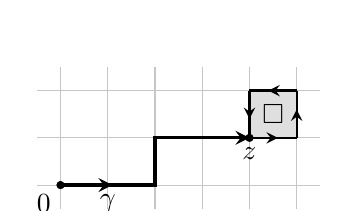
\begin{tikzpicture}[scale=0.6,>=stealth]
\draw[gray!45] (-0.5,-0.5) grid (5.5,2.5);
\fill[gray!25] (4,1) rectangle (5,2);
\draw[thick,->] (4,1)--(4.6,1); \draw[thick] (4.5,1)--(5,1);
\draw[thick,->] (5,1)--(5,1.6); \draw[thick] (5,1.5)--(5,2);
\draw[thick,->] (5,2)--(4.4,2); \draw[thick] (4.5,2)--(4,2);
\draw[thick,->] (4,2)--(4,1.4); \draw[thick] (4,1.5)--(4,1);
\node at (4.5,1.5) {$\square$};
\draw[very thick,->] (0,0)--(1.1,0); \draw[very thick] (1,0)--(2,0)--(2,1)--(3.1,1); \draw[very thick,->] (3,1)--(4,1);
\node[below] at (1,0) {$\gamma$};
\fill (0,0) circle (2.5pt) node[below left] {$0$};
\fill (4,1) circle (2.5pt) node[below] {$z$};
\end{tikzpicture}
\caption{A transported curvature $\sigma_{\gamma,\square}=\operatorname{Ad}(U_\gamma)F_\square(U)$, drawn in one coordinate plane: the curvature of the plaquette~$\square$ based at~$z$ is carried to the origin along the lattice path~$\gamma$.}\label{fig:A-transported}
\end{figure}

\subsection{Taylor-normalized sections}\label{sec:A-sections}

\begin{definition}[Local sections]\label{def:D19}
For a finite site stencil $\Sigma_d\subset\Z^4$, a local section has the form
\begin{equation*}
\localsection{d}[\mathbf c](U)=
\sum_{\nu,\mu}p_{\nu\mu}^{(d)}(\mathbf c)
\prod_{e,\alpha,\delta}U_e(\alpha,\delta)^{\nu_{e\alpha\delta}}\overline{U_e(\alpha,\delta)}^{\mu_{e\alpha\delta}}\,.
\end{equation*}
The product uses positive links with both endpoints in~$\Sigma_d$ and matrix indices $1\le\alpha,\delta\le n_G$. The sum is finite over nonnegative multi-indices; each coefficient is complex linear in~$\mathbf c$. The construction below chooses such a map to represent each continuum label.
\end{definition}

For a torus of side~$n_{\rm tor}$ (the side~$s$ of Definition~\ref{def:D02}), write $[x]$ for reduction of $x\in\Z^4$ modulo~$n_{\rm tor}$. Placement at a torus site~$y$ means evaluation on the periodic extension $U^{[y]}(x,a)=U(y+[x],a)$; denote it by $\localsection{d}[\mathbf c](y;U)$. On the cover, $\localsection{d}[\mathbf c](0;U)=\localsection{d}[\mathbf c](U)$. For $h\in\hypercubic$, define the configuration and jet actions by
\begin{align*}
(h^*U)(x,a)&=
\begin{cases}U(hx,b),&he_a=e_b,\\ U(hx-e_b,b)^{-1},&he_a=-e_b,\end{cases}\\
(h\mathsf j)_{j,a}(z)&=\sum_bh_{ab}\mathcal A_{j,b}(h^{-1}z),\qquad
(h\mathbf c)(\mathsf j)=\mathbf c(h^{-1}\mathsf j)\,.
\end{align*}
This action preserves homogeneity and radial gauge. Reality and covariance mean
\begin{equation*}
\localsection{d}[\overline{\mathbf c}](U)=\overline{\localsection{d}[\mathbf c](U)},\qquad
\localsection{d}[\mathbf c](h^*U)=\localsection{d}[h\mathbf c](U)\quad(h\in\hypercubic),
\end{equation*}
with conjugation as fixed above.

The following result supplies the sections specified in Section~\ref{sec:local-fields}; the unit normalization is exact at every configuration.
\begin{lemma}[Taylor-normalized sections]\label{lem:A1}
For every~$d$, a box stencil $\Sigma_d=[-\varrho_d,\varrho_d]^4\cap\Z^4$ and sections can be chosen gauge invariant, real and $\hypercubic$ covariant, with $\localsection{d}[\mathbf1]=1$, so that, for every $\mathbf c\in V_d$, radial jet~$\mathsf j$ and $0\le q\le d$,
\begin{equation}\label{eq:A-Taylor}
\left.\frac{d^q}{dh_{\rm lat}^q}\localsection{d}[\mathbf c](U(h_{\rm lat},\mathsf j))\right|_{h_{\rm lat}=0}
=\left.\frac{d^q}{dh_{\rm lat}^q}\mathbf c(\operatorname{sc}_{h_{\rm lat}}\mathsf j)\right|_{h_{\rm lat}=0}\,.
\end{equation}
\end{lemma}
Equivalently, $\taylormap_{d}\localsection{d}[\mathbf c]=\mathbf c$ for every $\mathbf c\in V_d$. The identity imposes no equality at positive spacing, and no compatibility between $\localsection{d}$ and $\localsection{d+1}$ is required. We fix the sections constructed in the following proof.

\begin{proof}
There are three steps: finitely many curvature measurements determine the truncated jet; an equivariant polynomial inverse of these measurements, composed with the label, gives a section with the right Taylor map; averaging over~$\hypercubic$ gives covariance and a common stencil. If $d<2$, the labels are constant and their constant sections suffice. Fix $d\ge2$.

\emph{Step 1: Curvatures determine the truncated jet.} The measurements $\sigma_{\gamma,\square}(U(1,\mathsf j))$ are smooth in~$\mathsf j$, and all links equal~$1$ at $\mathsf j=0$. The first variation of a link solution is the edge integral of the potential; that of a plaquette measurement is the circulation of the potential around the plaquette. Transport along~$\gamma$ contributes nothing at first order, because $F_\square(1)=0$. By the fundamental theorem of calculus on each edge, the circulation around the unit square at~$x$ in the plane of the axes $a<b$ is
\begin{equation*}
N_{ab}(x)=\int_0^1\!\int_0^1
(\partial_a\mathcal A_b-\partial_b\mathcal A_a)(x+\xi e_a+\eta e_b)\,d\xi\,d\eta\,.
\end{equation*}
Suppose all these linearized measurements vanish at $\mathcal A=\sum_{j=0}^{j_*}\mathcal A_j$. Then the polynomial~$N_{ab}$ vanishes on~$\Z^4$, hence identically: a polynomial vanishing on~$\Z^4$ is zero, by induction on the number of variables. The averaging shifts only lower the degree, so the homogeneous part of~$N_{ab}$ of degree~$j_*$ is $(\partial_a\mathcal A_{j_*,b}-\partial_b\mathcal A_{j_*,a})(x)$. It vanishes, and antisymmetry covers the other ordered pairs. Differentiating the radial condition and using Euler's identity gives
\begin{equation*}
(j_*+2)\mathcal A_{j_*,b}(z)=\sum_a z^a(\partial_a\mathcal A_{j_*,b}-\partial_b\mathcal A_{j_*,a})(z)=0\,.
\end{equation*}
Remove this component and descend in~$j_*$: the common kernel is zero. Adding a measurement whenever the kernel is nonzero decreases its dimension, so finitely many measurements $\sigma_1,\ldots,\sigma_{M_{\rm meas}}$ give a joint map
\begin{equation*}
\mathsf S:\mathcal J_{\le d}\longrightarrow\g^{M_{\rm meas}},\qquad
\mathsf S(\mathsf j)=(\sigma_l(U(1,\mathsf j)))_{l=1}^{M_{\rm meas}}
\end{equation*}
with injective derivative~$D\mathsf S(0)$.

\emph{Step 2: A polynomial inverse to the required order.} By uniqueness of the link equation, a constant gauge transformation $v\in G$ takes the test links of~$\mathsf j$ to those of~$\operatorname{Ad}(v)\mathsf j$, so~$\mathsf S$ is adjoint equivariant. The range of $D\mathsf S(0)$ is invariant; composing the inverse of $D\mathsf S(0)$ on it with orthogonal projection onto it gives an equivariant linear map $C:\g^{M_{\rm meas}}\to\mathcal J_{\le d}$ with $CD\mathsf S(0)=I$. By the inverse function theorem~\cite[Theorem~9.24]{Rudin1976}, $C\mathsf S$ has a local inverse~$\varphi$ near zero, smooth by differentiating $D\varphi=(D(C\mathsf S)\circ\varphi)^{-1}$. The adjoint actions are isometric, so $\varphi$ can be taken on invariant balls, where injectivity of~$C\mathsf S$ makes it equivariant. Put $f=\varphi\circ C$. Near zero, $f\mathsf S(\mathsf j)=\mathsf j$, $f(0)=0$ and $f(\operatorname{Ad}(v)z)=\operatorname{Ad}(v)f(z)$ for $v\in G$. Consequently the Taylor polynomial $T_df(z)=\sum_{k=1}^{d}D^kf(0)[z,\ldots,z]/k!$ is adjoint equivariant and has no constant term. Define
\begin{equation*}
Q_i(z)=b_{d,i}(T_df(z)),\qquad
\Psi_{\mathbf c}(U)=\sum_i c_iQ_i(\sigma_1(U),\ldots,\sigma_{M_{\rm meas}}(U))\,.
\end{equation*}
The polynomials~$Q_i$ are invariant and real on real arguments, and $Q_0=1$. If $b_{d,i}$ has factor count~$k_i$, every monomial of~$Q_i$ has at least~$k_i$ factors. Taylor's formula gives $T_df(\mathsf S(\mathsf j))=\mathsf j+O(|\mathsf j|^{d+1})$ near zero, hence
\begin{equation*}
\Psi_{\mathbf c}(U(1,\mathsf j))=\mathbf c(\mathsf j)+O_{\mathbf c}(|\mathsf j|^{d+1}),\qquad
\taylormap_{d}\Psi_{\mathbf c}=\mathbf c\,.
\end{equation*}
The polynomial~$Q_i$ itself need not have degree at most~$d$ in the curvature measurements.

\emph{Step 3: Covariance and a common stencil.} Average the section by
\begin{equation}\label{eq:A-average}
\localsection{d}[\mathbf c](U)=\frac1{|\hypercubic|}
\sum_{h\in\hypercubic}\Psi_{h^{-1}\mathbf c}(h^*U)\,.
\end{equation}
Changing the summation variable to $h'h$ proves $\localsection{d}[\mathbf c](h'^*U)=\localsection{d}[h'\mathbf c](U)$. Simultaneous adjoint covariance of the measurements gives gauge invariance. The real basis and the signed-permutation action give reality; the constant column remains one. The action preserves factor count, so averaging retains the lower bound on the number of curvature factors.

For a positive image direction, the pulled-back link equation has the coefficient of~$h^{-1}\mathsf j$, namely $h_{\rm lat}\sum_bh_{ba}\mathcal A_b^{\le d}(h_{\rm lat}h(x+se_a))$. Reversing the parameter and inverting the transport covers a negative image direction. Uniqueness gives $h^*U(h_{\rm lat},\mathsf j)=U(h_{\rm lat},h^{-1}\mathsf j)$. Each term of~\eqref{eq:A-average} therefore has Taylor map~$\mathbf c$. A signed image of a transported curvature is again a transported curvature, up to sign: reversal changes $F_\square$ to $-F_\square$, and a change of base point gives conjugation by the intervening boundary transport. Enclose the finitely many resulting paths and plaquettes in a box $\Sigma_d=[-\varrho_d,\varrho_d]^4\cap\Z^4$. This stencil contains zero and is signed-permutation invariant. Expanding the finite polynomial in matrix entries gives Definition~\ref{def:D19}. This proves~\eqref{eq:A-Taylor}, which is~\eqref{eq:I12-section-Taylor}.
\end{proof}

\subsection{Small-field bounds}\label{sec:A-bounds}

We bound normalized initial insertions using the ordered left derivatives of Definition~\ref{def:D05a}. At a placement~$y$, set $Y=y+[\Sigma_d]$; being healthy on~$Y$ means that every plaquette meeting~$Y$ has chord at most~$t$. A direction is permitted when
\begin{equation*}
|\dot{\mathcal A}_e|\le t(1+\operatorname{dist}(e^-,y))^\varpi\,.
\end{equation*}
Here $[\Sigma_d]$ is the torus image of the stencil, and $\operatorname{dist}(x,y)=\min_{z\in n_{\rm tor}\Z^4}|\tilde x-\tilde y+z|_\infty$ is the periodic maximum-coordinate distance, for any lifts $\tilde x,\tilde y$.
\begin{lemma}[Section bounds]\label{lem:A-bounds}
Each basis column is a polynomial in transported curvatures with at least~$k_i$ factors per monomial. For all $d,k,\varpi\in\N$ there are finite constants $C_{d,k,\varpi}$ and $C_d$ such that, on every torus, for every placement~$y$, $0<t\le1$, configuration healthy on~$Y$, and permitted direction list of length $q\le k$,
\begin{equation}\label{eq:A-section-bound}
\bigl|D^L_{\dot{\mathcal A}_1}\cdots D^L_{\dot{\mathcal A}_q}
\localsection{d}[b_{d,i}](y;U)\bigr|\le C_{d,k,\varpi}t^{k_i}\,.
\end{equation}
For arbitrary configurations,
\begin{equation}\label{eq:A-global-bound}
\sup_{i,y,U}|\localsection{d}[b_{d,i}](y;U)|\le C_d\,.
\end{equation}
\end{lemma}
Each curvature factor is at most of the size~$t$ of the plaquettes it reads, so a column with $k_i$ factors is of order~$t^{k_i}$ on healthy configurations. The proof uses the curvature polynomials constructed in Lemma~\ref{lem:A1}.
\begin{proof}
First note that $|F_\square(U)|\le\chord(U_\square)$: orthogonal projection is contractive and $\|U_\square-U_\square^*\|_{\rm F}\le2\|U_\square-1\|_{\rm F}$. Adjoint transport is isometric, so an undifferentiated curvature measurement is bounded by~$t$. An order-$q$ left derivative of a fixed path product is a finite sum of products of unitary matrices and exactly~$q$ direction matrices. On the fixed stencil their norms are at most a constant times~$t$, since periodic distance is bounded by cover distance. Thus each differentiated measurement is $O(t^q)$, and hence $O(t)$ when $q\ge1$. This argument also applies when cover links coincide after placement: one first differentiates the cover expression and then assigns the same direction to coincident links.

Apply the product rule to the curvature polynomials of~\eqref{eq:A-average}. Every differentiated monomial still has at least~$k_i$ factors, each bounded by a constant times~$t$. There are finitely many terms; since $t\le1$, their sum gives~\eqref{eq:A-section-bound}, including order zero. Each entry of a unitary matrix has absolute value at most one, so the finite matrix-entry polynomial gives~\eqref{eq:A-global-bound}. The formula also gives smoothness, measurability and locality. The constants depend on the sections, $G,d,k,\varpi$ as applicable, and finite maxima make them nondecreasing in the integer parameters. They are fixed before the stage block ratios in Section~\ref{sec:constants}.
\end{proof}

By linearity, Lemma~\ref{lem:A-bounds} bounds permitted derivatives of $\localsection{d}[t^{-\factorcount}\mathbf c]$ by $C_{d,k,\varpi}\sum_i|c_i|$ on the healthy set: the factor $t^{-k_i}$ cancels $t^{k_i}$. Taking $t=t_N$, $k=\mathfrak q_{J_N}$ and $\varpi=\varpi_{J_N}$ bounds the initial marked density of~\eqref{eq:I12-marked-evolution} on the healthy set, in the sense of Definition~\ref{def:D05a}. On unhealthy configurations the global bound gives $C_d\sum_i|c_i|t^{-k_i}$; the proof of Lemma~\ref{lem:E2.1} places this contribution in a merged forced remainder of~\eqref{eq:I12-marked-representation}.

\subsection{Auxiliary equation sections}\label{sec:A-equations}

Exact lattice equation identities require different sections, still polynomial and local with the same small-field bounds. On~$\mathcal J_j$ define the Maxwell subspace and the equation labels by
\begin{equation*}
\mathcal J_j^{\rm Max}=\Bigl\{\mathcal A_j:\ \sum_a\partial_a(\partial_a\mathcal A_{j,b}-\partial_b\mathcal A_{j,a})=0\ \text{for every }b\Bigr\},\qquad
\mathcal I_d=\Bigl\{p\in V_d:p|_{\prod_j\mathcal J_j^{\rm Max}}=0\Bigr\}\,.
\end{equation*}
Here restriction uses only $j+2\le d$. Substitution into $\prod_j\mathcal J_j^{\rm Max}$ preserves bidegree, so $\mathcal I_d$ is the direct sum of its bihomogeneous parts. Order bidegrees~$(w,k)$ by the lexicographic order of~$(k,w)$. A triangular regrading (a unipotent change of labels) is a complex-linear map on~$V_d$ whose difference from the identity sends each bihomogeneous polynomial into strictly later bidegrees. There are finitely many bidegrees, so this difference is nilpotent and the map is invertible; the map and its inverse preserve the filtration by minimum factor count.

\paragraph{Idea: free equations in an interacting theory.} Haar integration by parts in one link, a lattice Schwinger--Dyson identity, shows that for $\beta\ne0$ the force~$\mathcal E_e$ of~\eqref{eq:A-link-equation}, the derivative of the Wilson energy in the link~$e$, has zero moments when multiplied by a function independent of~$U_e$ and by observables of distant links. Its linearization is the divergence of the linearized curvature, and the Maxwell equations enter only through this linearization. An equation label is a sum of products with one factor vanishing on Maxwell jets. Replacing that factor by forces and the others by curvature measurements gives an observable with exactly vanishing exterior moments, whose Taylor map is the label plus later terms, produced by the higher-weight linear terms of the lattice force and by nonlinear corrections. The construction therefore exhibits exact lattice equations for the labels in~$\mathsf R_d(\mathcal I_d)$: this is the lattice form of the vanishing of equation-of-motion operators at separated points. For example, put $F_{ab}=\partial_a\mathcal A_{0,b}-\partial_b\mathcal A_{0,a}$ and $(\partial\cdot F)_b=\sum_c\partial_c(\partial_c\mathcal A_{1,b}-\partial_b\mathcal A_{1,c})$, both constant. The label $q_{\rm eq}=\sum_b\langle(\partial\cdot F)_b,(\partial\cdot F)_b\rangle_\g$ lies in~$\mathcal I_6$ and has bidegree $(6,2)$. The only later bidegree of weight at most six is~$(6,3)$, so $\mathsf R_6q_{\rm eq}-q_{\rm eq}$ is a cubic invariant polynomial in the~$F_{ab}$; nothing below requires it to vanish. The equation count is shared with the free theory, the separated correlations are not: Proposition~\ref{prop:FC} and~\eqref{eq:E-equation-count} give $\dim\nullspace{d}(S)=\dim\mathcal I_d$, while in the selected phase $\tracetwopoint$ is asymptotic to $\traceamplitude r^{-8}\log^{-2}(1/r)$ (Theorem~\ref{prop:TR}), and on no interval $(0,\delta)$ does $\tracetwopoint$ agree with a finite Wick profile (Proposition~\ref{prop:NF}).

\paragraph{Lattice symmetries.} We record the symmetries of the Wilson measure deferred from Definition~\ref{def:D02}. A site gauge transformation acts on plaquette holonomies by conjugation, and an affine isometry $h_{\rm iso}(x)=hx+b$ with $h\in\hypercubic$ by conjugation, possibly after inversion; both preserve~$\wilsonterm$. Product probability Haar measure is invariant under fixed left and right multiplication, inversion and permutation~\cite[Corollary~2.28 and Proposition~2.31]{Folland2015}. Hence, for every integer side $n_{\rm tor}\ge1$, real~$\beta$, site gauge transformation~$\gamma_{\rm g}$ and bounded measurable~$F$,
\begin{equation}\label{eq:A-Wilson-invariance}
\int F(U^{\gamma_{\rm g}})\,d\mu_{n_{\rm tor},\beta}(U)
=\int F(h_{\rm iso}^*U)\,d\mu_{n_{\rm tor},\beta}(U)
=\int F(U)\,d\mu_{n_{\rm tor},\beta}(U)\,.
\end{equation}

For a torus site~$y$, put $\mathbb B_r(y)=\{x:\operatorname{dist}(x,y)\le r\}$. An exterior spectator outside~$\mathbb B_r(y)$ is a bounded measurable function of the positive links having both endpoints outside~$\mathbb B_r(y)$; it need not be gauge invariant. The following identity supplies the auxiliary equation observables used in Section~\ref{sec:partII-E}.
\begin{lemma}[Auxiliary equation sections]\label{lem:A-R4}
For every~$d$ there are a local section~$V_d^{\rm aux}$ as in Definition~\ref{def:D19}, an invertible triangular regrading~$\mathsf R_d$ of~$V_d$, and $r_d,M_d\in\N$ with the following properties.
\begin{enumerate}[label=\textup{(\roman*)},nosep]
\item The section has its own box stencil, is gauge invariant, real and $\hypercubic$ covariant, satisfies $V_d^{\rm aux}[\mathbf1]=1$ and~\eqref{eq:A-Taylor}, and satisfies \eqref{eq:A-section-bound}--\eqref{eq:A-global-bound} with its own constants.
\item The map~$\mathsf R_d$ fixes~$\mathbf1$ and commutes with conjugation and~$\hypercubic$.
\item For every $n_{\rm tor}\ge M_d$, $\beta\ne0$, placement~$y$, $p\in\mathcal I_d$ and exterior spectator~$F_{\rm ext}$ outside~$\mathbb B_{r_d}(y)$,
\begin{equation}\label{eq:A-aux-zero}
\int V_d^{\rm aux}[\mathsf R_dp](y;U)F_{\rm ext}(U)\,d\mu_{n_{\rm tor},\beta}(U)=0\,.
\end{equation}
\end{enumerate}
\end{lemma}
The exact-equation subspace $\mathsf R_d(\mathcal I_d)$ is compared with the selected primary family in Section~\ref{sec:partII-E}. All choices in the following proof depend only on~$G,d$ and the label basis.

\begin{proof}
There are three steps: one-link integration by parts gives zero moments; forces realize every linear functional vanishing on Maxwell jets; products of forces and curvature measurements, averaged, represent equation labels up to a triangular regrading, which is then inverted.

\emph{Step 1: One-link equations.} Extend the curvature $F_\square$ of Section~\ref{sec:A-labels} to $F_{ab}(U;x)$ for ordered axes by antisymmetry, with $F_{aa}=0$. For a positive link $e=(x,a)$ set
\begin{equation*}
\mathcal E_e(U)=\sum_{b\ne a}\left(F_{ab}(U;x)-\operatorname{Ad}(U(x-e_b,b)^{-1})F_{ab}(U;x-e_b)\right)\,.
\end{equation*}
On a torus of side at least two, direct differentiation gives
\begin{equation}\label{eq:A-link-equation}
D^L_{e,A}E^{\rm W}(U)=\langle A,\mathcal E_e(U)\rangle_{\g}\,.
\end{equation}
Indeed, the forward plaquette contributes $-n_G^{-1}\operatorname{Re}\tr(AU_\square)=\langle A,F_\square\rangle_{\g}$. The backward plaquette, rebased at~$x$, contributes the negative of the transported curvature in the display. These are the two incidences for each transverse axis; antisymmetry gives the signs for the opposite ordering.

If a continuous multiplier~$g$ is independent of~$U_e$, and a bounded measurable~$F_{\rm ext}$ is also independent of~$U_e$, left invariance of Haar measure gives
\begin{equation*}
0=\left.\frac{d}{d\epsilon}\int g(U)F_{\rm ext}(U)e^{-\beta E^{\rm W}(U^{e,A,\epsilon})}\,dU\right|_{\epsilon=0}
=-\beta Z_{n_{\rm tor},\beta}\int\langle A,\mathcal E_e\rangle_{\g}gF_{\rm ext}\,d\mu_{n_{\rm tor},\beta}\,.
\end{equation*}
Here $U^{e,A,\epsilon}_e=e^{\epsilon A}U_e$ and all other links are fixed. Compactness bounds the derivative of the smooth density uniformly, justifying differentiation even for measurable~$F_{\rm ext}$.

Choose a path~$\gamma_e$ from~$0$ to~$e^-$ avoiding~$e$. If~$g$ also avoids~$e$, then
\begin{equation*}
\Upsilon_{e,\xi}(U)=\langle \xi,\operatorname{Ad}(U_{\gamma_e})\mathcal E_e(U)\rangle_{\g}g(U)
\end{equation*}
has zero moment for every $\xi\in\g$ against every exterior spectator. To see this, expand $\operatorname{Ad}(U_{\gamma_e}^{-1})\xi$ in a fixed orthonormal basis of~$\g$ and apply the preceding identity to each coefficient times~$gF_{\rm ext}$. These multipliers are independent of~$U_e$. There is one radius and one minimum torus side for any finite collection of such expressions: enlarge the radius to contain both endpoints of every varied link, and the side until distinct links in their finite cover supports remain distinct after wrapping. The same choices work at every placement.

\emph{Step 2: Enough measurements with avoidance.} Any path can avoid one specified link: replace a traversal of that link by three sides of a square in a transverse direction. For each plaquette orientation only finitely many base points give a plaquette containing that link. Removing these points does not affect Step~1 of the proof of Lemma~\ref{lem:A1}: if a polynomial vanishes at all but finitely many points of~$\Z^4$, its restriction to each coordinate line through an integer point has infinitely many zeros, so it vanishes on~$\Z^4$ and hence identically. Thus curvature measurements whose paths and plaquettes avoid~$e$ still have injective joint linearization. Finite-dimensional duality therefore realizes every linear functional on~$\mathcal J_{\le d}$ by finitely many components.

For every linear functional~$\ell$ on~$\mathcal J_j$ vanishing on~$\mathcal J_j^{\rm Max}$, a finite combination of force linearizations equals $\mathsf j\mapsto\ell(\mathcal A_j)$ on $\mathcal J_{\le j+2}=\bigoplus_{i\le j}\mathcal J_i$. To see this, extend the circulations~$N_{ab}$ of Step~1 of the proof of Lemma~\ref{lem:A1} antisymmetrically. The force linearization at~$e=(x,a)$ is
\begin{equation*}
L_a(\mathsf j;x)=\sum_b\bigl(N_{ab}(x)-N_{ab}(x-e_b)\bigr)\,.
\end{equation*}
Suppose that every $L_a(\mathsf j;x)$, $x\in\Z^4$, vanishes for a jet $\mathcal A=\sum_{i\le j_*}\mathcal A_i$. Each $L_a(\mathsf j;\cdot)$ is a polynomial, hence zero. In $N_{ab}(x)-N_{ab}(x-e_b)$ a component~$\mathcal A_i$ contributes a polynomial of degree at most~$i-1$, and $\mathcal A_{j_*}$ contributes $\partial_b(\partial_a\mathcal A_{j_*,b}-\partial_b\mathcal A_{j_*,a})(x)$ plus terms of lower degree. The part of degree~$j_*-1$ therefore gives $\sum_b\partial_b(\partial_a\mathcal A_{j_*,b}-\partial_b\mathcal A_{j_*,a})=0$, that is, $\mathcal A_{j_*}\in\mathcal J_{j_*}^{\rm Max}$. A functional of this top component annihilating~$\mathcal J_{j_*}^{\rm Max}$ therefore annihilates the common kernel of the force measurements. Finite-dimensional duality puts it in their linear span. Transport paths do not enter the linearization and can be chosen to avoid their varied links. On~$\mathcal J_{\le d}$ the same combination can have additional linear terms only at engineering weights above~$j_*+2$.

\emph{Step 3: Polynomial lifts and the triangular map.} Choose linear projections $\pi_j:\mathcal J_j\to\mathcal J_j^{\rm Max}$ and put $\pi=\prod_j\pi_j$. A polynomial belongs to~$\mathcal I_d$ precisely when $p\circ\pi=0$. For a product of linear coordinates,
\begin{equation*}
\prod_{i=1}^{k_{\rm tot}}\ell_i-\prod_{i=1}^{k_{\rm tot}}(\ell_i\circ\pi)
=\sum_{i=1}^{k_{\rm tot}}\left[\prod_{l<i}(\ell_l\circ\pi)\right]
(\ell_i-\ell_i\circ\pi)\prod_{l>i}\ell_l\,.
\end{equation*}
Consequently every bihomogeneous equation label is a finite sum of products with one linear factor vanishing on some~$\mathcal J_j^{\rm Max}$, with the same engineering weight and factor count. The individual factors need not be invariant. We use the Taylor map~$\taylormap_{d}$ of Section~\ref{sec:A-labels}; every coordinate has weight at least two. Call a lattice observable~$O$ a lift of a bihomogeneous polynomial~$q$ if $\taylormap_{d}O-q$ consists of monomials later than~$q$ in the $(k,w)$ order.

Lift the distinguished factor by a finite combination of transported forces from Step~2. For each summand, lift the other factors by curvature measurements avoiding its varied link, matching their full linear parts through engineering weight~$d$. The resulting expression has the zero-moment property of Step~1 and at least~$k_{\rm tot}$ curvature factors. Indeed, every force is a difference of two transported curvatures per transverse axis. The expression is a lift of the prescribed product: the additional linear terms of the force have greater engineering weight, and every nonlinear correction increases factor count. The square-measurement lifts have their prescribed full linear parts, so introduce only the latter kind of correction. Taylor polynomials exist by the smooth dependence of the test holonomies on the jet.

Average over constant gauge transformations. All factors transform by adjoint matrices at the origin, so the orbit lies in the finite-dimensional span of finitely many fixed-degree colour-coordinate monomials on the same measurements; each orbit function keeps zero moments, with colour vectors rotated by $\operatorname{Ad}(v^{-1})$. The Haar average is therefore a gauge-invariant finite combination of orbit functions; it keeps zero moments, minimum factor count and the lift property, and its Taylor map is invariant.

In each bidegree extend a basis of~$\mathcal I_d$ to a basis of the invariant label space in that bidegree, lifting the complementary vectors by Lemma~\ref{lem:A1}. Lift~$\mathbf1$ to~$1$, since $\mathcal I_d$ contains no nonzero constant. Summing gives a linear lift~$p\mapsto\mathcal Y_p$. Replace this lift by the two successive averages
\begin{align*}
\mathcal Y'_p(U)&=\frac1{|\hypercubic|}\sum_{h\in\hypercubic}\mathcal Y_{h^{-1}p}(h^*U),\\
\mathcal Y^{\rm sym}_p&=\frac12\left(\mathcal Y'_p+\overline{\mathcal Y'_{\bar p}}\right)\,.
\end{align*}
The Taylor map commutes with both operations. The real Maxwell equations and the chain rule make $\mathcal J_j^{\rm Max}$, and hence~$\mathcal I_d$, stable under signed permutations, adjoint transformations and conjugation. The zero-moment property survives the signed average by~\eqref{eq:A-Wilson-invariance}, changing the spectator by the inverse isometry; the exterior set is preserved. Conjugation uses~$\overline{F_{\rm ext}}$. A reversed varied link uses a right derivative of the Wilson energy, whose Haar identity is identical. Thus the averaged equation representatives remain finite sums of one-link action derivatives with link-independent multipliers and avoiding transport paths.

Let $\mathsf R_dp=\taylormap_{d}\mathcal Y^{\rm sym}_p$. Then $\mathsf R_d-I$ strictly raises~$(k,w)$. There are finitely many bidegrees of weight at most~$d$, so $(\mathsf R_d-I)^{n_0}=0$ for some integer~$n_0$, and
\begin{equation*}
\mathsf R_d^{-1}=\sum_{l=0}^{n_0-1}(-1)^l(\mathsf R_d-I)^l,\qquad
V_d^{\rm aux}[\mathbf c]=\mathcal Y^{\rm sym}_{\mathsf R_d^{-1}\mathbf c}\,.
\end{equation*}
This gives invertibility and Taylor normalization; the averages give the symmetry and unit identities. The inverse preserves minimum factor count, so Lemma~\ref{lem:A-bounds} applies to these sections with their own constants. A signed-invariant box enclosing all paths and plaquettes gives a common stencil. Take $r_d,M_d$ as maxima for an ideal basis; linearity gives~\eqref{eq:A-aux-zero}.
\end{proof}

\subsection{Example: the curvature square}\label{sec:A-example}

We follow one familiar observable through the construction. Sections~\ref{sec:partII-E} and~\ref{sec:partII-F} construct the terminal map and the quotient used at its end.

\paragraph{The label.} With $F_{ab}$ as in Section~\ref{sec:A-equations}, radial gauge gives $\mathcal A_{0,a}(x)=\frac12\sum_bx^bF_{ba}$; since $\mathcal A(0)=0$, $F_{ab}$ is the curvature of the jet at the origin. The curvature square is the label
\begin{equation*}
c_{F^2}(\mathsf j)=\frac14\sum_{a,b}\langle F_{ab},F_{ab}\rangle_\g=\frac14\sum_{a,b,\alpha}(F_{ab}^\alpha)^2\,,
\end{equation*}
with coordinates~$F^\alpha_{ab}$ in an orthonormal basis of~$\g$: the Yang--Mills density at the origin. It is invariant, real and $\hypercubic$ invariant, of bidegree $(4,2)$, and lies in~$V_d$ for every $d\ge4$.

\paragraph{Two lattice readings.} For $a<b$ and $s,s'=\pm1$, let $\square_{ab}^{ss'}$ be the plaquette with corner~$0$ spanned by~$se_a$ and~$s'e_b$. The clover
\begin{equation*}
P^{\rm cl}(U)=\frac14\sum_{a<b}\sum_{s,s'=\pm1}\wilsonterm(U_{\square_{ab}^{ss'}})
\end{equation*}
satisfies $\taylormap_{4}P^{\rm cl}=c_{F^2}$. Indeed, on test holonomies each of these plaquettes has $U_\square=e^X$ with $X=\pm h_{\rm lat}^2F_{ab}+O(h_{\rm lat}^3)\in\g$, and $\wilsonterm(e^X)=\frac12\langle X,X\rangle_\g+O(|X|^3)$ because $\operatorname{Re}\tr X=0$; hence $P^{\rm cl}(U(h_{\rm lat},\mathsf j))=h_{\rm lat}^4c_{F^2}(\mathsf j)+O(h_{\rm lat}^5)$. This familiar leading-order reading is gauge invariant, real and $\hypercubic$ invariant, and at most~$3t^2$ when its plaquettes have chord at most~$t$: the size~$t^{k_i}$, $k_i=2$, of Lemma~\ref{lem:A-bounds}. The column $\localsection{4}[c_{F^2}]$ of Lemma~\ref{lem:A1} is built differently, as the $\hypercubic$ average of $c_{F^2}(T_4f(\sigma_1,\ldots,\sigma_{M_{\rm meas}}))$: it recovers the truncated jet from curvature measurements and evaluates the label on it. The two differ by an observable with vanishing Taylor map; the terminal map below refers to the section of Lemma~\ref{lem:A1}.

\paragraph{The insertion.} Take $d=4$. A nonconstant monomial of weight at most four is a coordinate of~$\mathcal A_0$, $\mathcal A_1$ or~$\mathcal A_2$, or a product of two coordinates of~$\mathcal A_0$, and invariant linear terms vanish because $\g$ is simple. As the adjoint representation is absolutely irreducible, every label in~$V_4$ is $m_0\mathbf1+\sum_{P,Q}m_{PQ}\langle F_P,F_Q\rangle_\g$, summed over coordinate planes, with $m$ symmetric. A reflection of one axis changes the sign of~$F_P$ exactly for the planes containing that axis. Hence $\hypercubic$ invariance forces~$m$ to be diagonal and, by permutations, constant: the real $\hypercubic$ invariant labels in~$V_4$ are the real combinations of~$\mathbf1$ and~$c_{F^2}$. For $N\ge\reflevel{4}$, Lemma~\ref{lem:E2.1a} makes $\mathsf Z_{N,p,4}$ commute with conjugation and~$\hypercubic$, and gives $\mathsf Z_{N,p,4}\mathbf1=(a_{\reflevel{4}}/a_N)^4\mathbf1$. The fine-cutoff coefficient vector and, by Definition~\ref{def:D08}, the insertion are therefore
\begin{align*}
\mathsf Z_{N,p,4}^{-1}c_{F^2}&=\lambda_{N,p}c_{F^2}+\delta^{F^2}_{N,p}\mathbf1\,,\\
O^{(4)}_{N,p}(c_{F^2},y;U)&=a_N^{-4}\bigl(\lambda_{N,p}t_N^{-2}\localsection{4}[c_{F^2}](y;U)+\delta^{F^2}_{N,p}\bigr)\,,
\end{align*}
with real $\delta^{F^2}_{N,p}$ and real $\lambda_{N,p}\ne0$, since $\mathsf Z_{N,p,4}$ preserves~$\C\mathbf1$. The renormalization of the curvature square is a multiplicative constant together with an additive one.

Mixing enters through the transfer: the representation~\eqref{eq:I12-marked-representation} of the blocked marked density keeps a unit coordinate~$x_{m,0}$, through which integration can turn part of a curvature insertion into a constant. The inverse terminal map makes the transported coefficient at the reference level exactly~$c_{F^2}$, with unit coordinate zero, which specifies the label at the physical scale~$a_{\reflevel{4}}$. A single factor ($\delta^{F^2}_{N,p}=0$) would require the transfer to preserve the line through~$c_{F^2}$, and nothing in the construction forces this. In degree six, $\mathsf Z_{N,p,6}^{-1}c_{F^2}$ may involve every real $\hypercubic$ invariant label of weight at most six, including any that are not rotation invariant.

The degree tag acts separately from weight and factor count: it fixes~$\ell_m^d$, $a_N^{-d}$ and the terminal map. Thus $(4,c_{F^2})$ and $(6,c_{F^2})$ are different insertion labels; the inclusion $\jmath_{4,6}$ of Proposition~\ref{prop:FC} maps the class of the first to the class in~$F_6$ with the same correlations, which need not be the class of the second.

\paragraph{The field.} Degree four has no invisible labels. Labels in~$V_4$ depend only on~$\mathcal A_0$, and $\mathcal J_0^{\rm Max}=\mathcal J_0$ because the curvature of~$\mathcal A_0$ is constant; so $\mathcal I_4=0$, and~\eqref{eq:E-equation-count} with Proposition~\ref{prop:FC} gives $\dim F_4=\dim V_4$. Thus $\nullspace{4}(S)=0$, the quotient map $V_4\to F_4$ is bijective, and $[c_{F^2}]\ne0$. In each phase~$\xi$, Theorem~\ref{prop:RC} gives the smeared field $\Phi_\xi(\iota_4[c_{F^2}],f)$. Its free counterpart is the Maxwell curvature square~$\curvaturesquare$ of Section~\ref{sec:trace-products}, whose two-point function at separation~$r$ is $3\dimG\pi^{-4}r^{-8}$; Section~\ref{sec:partII-I} compares the stress trace with it.

\section{Gauges and block integration}\label{sec:partII-B}

The block map of Definition~\ref{def:D04} sends a fine-field density to a coarse-field density: it integrates over the fine links $U$, while its kernel integrates to one over the coarse links $V$ for each fixed~$U$. The predictor in that kernel averages fine parallel transports in local frames. A fixed axial frame would distinguish an ordering of the axes. We instead minimize a symmetric average of transport energies when the field is sufficiently small, and average over curvature-controlled axial frames elsewhere. Section~\ref{subsec:B-kernel} shows that these choices give a measurable, covariant probability kernel; consequently the block integration in Theorem~\ref{prop:RG} preserves the partition function.

The remaining subsections prepare the small-field integration used in Sections~\ref{sec:partII-C} and~\ref{sec:partII-D}. Section~\ref{subsec:B-free} solves the free block problem: the free action at every level, the free interpolation~$W_0$ from coarse to fine fields, and an exact square completion. Section~\ref{subsec:B-stationary} constructs the stationary fine field about a coarse field and integrates the Gaussian fluctuations about it; the determinant, the Haar Jacobian and the inherited loop action form the one-loop action~$\mathsf T$. Section~\ref{subsec:B-inverse} supplies what Section~\ref{sec:partII-C} needs to extract the curvature-square coefficient of~$\mathsf T$: inverse bounds uniform in the block ratio, vertex bounds whose input-dependent part carries a factor~$\ell^{-1}$, and a Ward identity showing that the predictor contact term (the chain-rule term containing the second derivative of the predictor) does not change that coefficient. Sections~\ref{subsec:B-energy} and~\ref{subsec:B-sector} give the local large-field energy (Lemma~\ref{lem:B-D1}) and the simultaneous differentiated local integral (Lemma~\ref{lem:B-D2}) used in Section~\ref{sec:partII-D}.

Three uniformities require care.
\begin{enumerate}[label=(\roman*)]
\item The frame and predictor cutoffs must work on patches with arbitrarily many sites. Centred frame minimizers satisfy a contraction whose constant does not depend on the patch (Lemma~\ref{lem:B1}).
\item The free kernels must stay controlled after arbitrarily many blockings. We separate the principal Fourier pole before inverting (Lemma~\ref{lem:B2}).
\item The determinant comparison must not see the $\ell^4$ sites of a fine cell. The difference of the two compared operators either factors through coarse spaces or contains the regulator $\mathfrak m_\mu=\mu^2(P_\mu^3)^3$, and $P_\mu^3$ is trace class uniformly in~$\ell$ (Lemmas~\ref{lem:B7} and~\ref{lem:C6}).
\end{enumerate}

\paragraph{Induction scheme.}
Sections~\ref{sec:partII-B}--\ref{sec:partII-D} prove one descending induction on~$m$, started at $m=N$ by the Wilson representation of Lemma~\ref{lem:D3}. The hypothesis of the step $m+1\to m$ has two parts: the path bounds and cancellations of Lemmas~\ref{lem:C1}--\ref{lem:C2} at level $m+1$, for the input path action of Definition~\ref{def:D23}; and an input curve satisfying Definitions~\ref{def:D24}--\ref{def:D25a} and~\eqref{eq:I12-activity-caps}. The stationary integration of this section and the determinant comparison of Section~\ref{sec:partII-C} first construct the level-$m$ path arrays; the joint proof after Lemma~\ref{lem:C7} shows that they satisfy Lemmas~\ref{lem:C1}--\ref{lem:C2} at level~$m$. Lemmas~\ref{lem:D1} and~\ref{lem:D5} construct the output activities. Lemma~\ref{lem:C8} then fixes the output coupling; its proof uses Lemmas~\ref{lem:D4}, \ref{lem:D1}, \ref{lem:D5} and~\ref{lem:D6}, none of which uses Lemma~\ref{lem:C8}. Lemma~\ref{lem:D2} closes the step. Curl division (Lemma~\ref{lem:C3}) and gauge completion (Lemma~\ref{lem:C5}) do not use the induction.

Throughout, use the group and metric of Definition~\ref{def:D01}, the Wilson term~\eqref{eq:I12-price-chord}, and the level choices~\eqref{eq:I12-levels}. At a step $m+1\to m$, put $j=J_{m+1}$, $\ell=\ell_m$ and $R=(j+3)\ell$. Unless stated otherwise, periods satisfy the minimum-period requirement in Section~\ref{sec:constants}. All finite operators use counting inner products and are periodizations of the kernels described below. An adjoint at complex momentum means the analytic continuation of the real-momentum adjoint.

\subsection{The block kernel}\label{subsec:B-kernel}

Before averaging transports, we express them in common endpoint frames. When the resulting connectors lie close to one another in~$G$, their weighted average lies close to~$G$, and its nearest point of~$G$ serves as a group-valued average. The other branches complete the kernel on the remaining configurations. Figure~\ref{fig:B-predictor} shows the two cases, and Table~\ref{tab:B-branches} lists the tests.

\begin{figure}[ht]
\centering
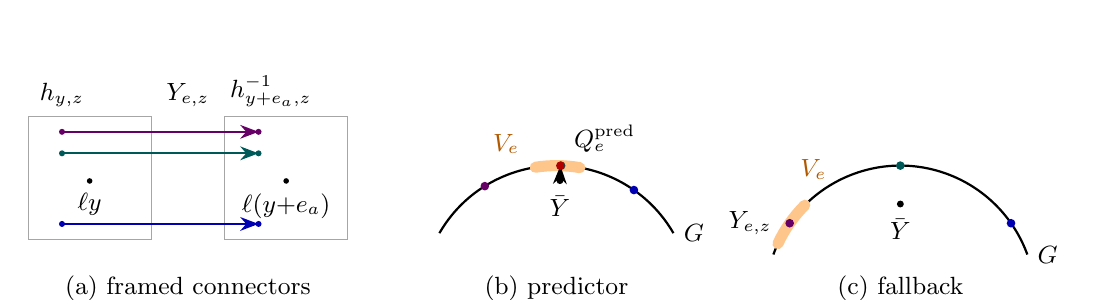
\begin{tikzpicture}[scale=0.78,>=Stealth,font=\small]
\begin{scope}
 \draw[gray!70] (0,0) rectangle (2,2);
 \draw[gray!70] (3.2,0) rectangle (5.2,2);
 \fill (1,0.95) circle (1.3pt) node[below=1pt] {$\ell y$};
 \fill (4.2,0.95) circle (1.3pt) node[below=1pt] {$\ell(y{+}e_a)$};
 \foreach \yy/\c in {0.25/blue!70!black,1.4/teal!70!black,1.75/violet!80!black}{
   \draw[\c,thick,->] (0.55,\yy) -- (3.75,\yy);
   \fill[\c] (0.55,\yy) circle (1.4pt);
   \fill[\c] (3.75,\yy) circle (1.4pt);}
 \node[above] at (0.55,2.0) {$h_{y,z}$};
 \node[above] at (3.95,2.0) {$h_{y+e_a,z}^{-1}$};
 \node[above] at (2.6,2.0) {$Y_{e,z}$};
 \node at (2.6,-0.8) {(a) framed connectors};
\end{scope}
\begin{scope}[xshift=8.6cm,yshift=-1.0cm]
 \coordinate (O) at (0,0);
 \draw[thick] (150:2.2) arc (150:30:2.2) node[right] {$G$};
 \foreach \a/\n in {55/A,88/B,122/C}{\coordinate (\n) at (\a:2.2);}
 \coordinate (Yb) at ($0.3333*(A)+0.3333*(B)+0.3334*(C)$);
 \coordinate (Q) at ($(O)!2.2cm!(Yb)$);
 \draw[line width=4pt,orange!45,line cap=round] (80:2.2) arc[start angle=80, end angle=99, radius=2.2];
 \foreach \n/\c in {A/blue!70!black,B/teal!70!black,C/violet!80!black}{\fill[\c] (\n) circle (2pt);}
 \fill (Yb) circle (1.6pt) node[below=2pt] {$\bar Y$};
 \draw[->,dashed,thick] (Yb) -- (Q);
 \fill[red!70!black] (Q) circle (2pt);
 \node[above right=2pt] at (Q) {$Q^{\rm pred}_e$};
 \node[orange!70!black,above left=2pt] at (100:2.2) {$V_e$};
 \node at (90:0.2) {(b) predictor};
\end{scope}
\begin{scope}[xshift=14.2cm,yshift=-1.0cm]
 \coordinate (O) at (0,0);
 \draw[thick] (160:2.2) arc (160:20:2.2) node[right] {$G$};
 \foreach \a/\n in {35/A,90/B,145/C}{\coordinate (\n) at (\a:2.2);}
 \coordinate (Yb) at ($0.3333*(A)+0.3333*(B)+0.3334*(C)$);
 \draw[line width=4pt,orange!45,line cap=round] (135:2.2) arc[start angle=135, end angle=155, radius=2.2];
 \foreach \n/\c in {A/blue!70!black,B/teal!70!black,C/violet!80!black}{\fill[\c] (\n) circle (2pt);}
 \fill (Yb) circle (1.6pt) node[below=2pt] {$\bar Y$};
 \node[left=3pt] at (145:2.2) {$Y_{e,z}$};
 \node[orange!70!black,above=3pt] at (130:2.2) {$V_e$};
 \node at (90:0.2) {(c) fallback};
\end{scope}
\end{tikzpicture}
\caption{The predictor of a coarse link $e=(y,a)$. (a) Fine connectors between two blocks, each expressed in the frames at its two endpoints. (b) When the connectors lie close together in~$G$, their weighted average $\bar Y=\sum_zw^{\rm av}_zY_{e,z}$ is a matrix just off~$G$; the predictor is its nearest point of~$G$, and the coarse link~$V_e$ fluctuates about it with weight $e^{-\blockpenalty\beta\wilsonterm(V_eQ_e^{-1})}$. (c) When the connectors are spread out, a single connector $Y_{e,z}$ is chosen with probability $w^{\rm av}_z$ and $V_e$ fluctuates about it. This branch is part of the definition of the kernel on every configuration where the minimum test fails.}\label{fig:B-predictor}
\end{figure}

For $o\in S_4$, let $T_U(y\to z;o)$ be the ordered product along the path that changes the four coordinates in the order~$o$, using inverse links for negative steps.
\begin{definition}[Axial frames]\label{def:D20a}
The frame tagged by $(z,o)$, its normalization and its link coordinates are
\begin{equation*}
g_y^{z,o}=T_U(z\to y;o),\qquad h_y^{z,o}=(g_0^{z,o})^{-1}g_y^{z,o},\qquad
U_{(y,a)}^{z,o}=g_y^{z,o}U(y,a)(g_{y+e_a}^{z,o})^{-1}\,.
\end{equation*}
These frames provide the finite alternatives for the symmetric gauge choice.
\end{definition}

In the patch $\ell y+\mathbb B_R$ we abbreviate the frame $h_{y,r}$ of~\eqref{eq:I12-framed-connector} at offset~$r\in\mathbb B_R$ to~$h_r$. Here $\delta_{\rm fr}>0$ is the frame cutoff and $a_{\rm ax}\ge16$ the axial factor of item~2 of Table~\ref{tab:constant-choices}; patch sums count internal positive links and plaquettes. The frame test below compares transports around loops through the patch centre: under a gauge transformation such a loop transport is conjugated, so its chord is gauge invariant.
\begin{definition}[Symmetric frame choice]\label{def:D20b}
For $x,y\in\mathbb B_R$ and $o,o_0\in S_4$ let $\mathcal T_{xy;o}^{o_0}=g_x^{0,o_0}T_U(x\to y;o)(g_y^{0,o_0})^{-1}$, the transport from $0$ to~$x$ in order~$o_0$, then to~$y$ in order~$o$, then back to~$0$ along the reversed route of order~$o_0$. Tags lie in $\mathbb B_R\times S_4$.
\begin{enumerate}[label=(\alph*)]
\item\emph{Minimizing branch.} If $\chord(\mathcal T_{xy;o}^{o_0})<\delta_{\rm fr}$ for all $x,y,o,o_0$, the frame $(h_r)_{r\in\mathbb B_R}$ is the minimizer with $h_0=1$ of
\begin{equation*}
\frac1{24|\mathbb B_R|^2}\sum_{r,r'\in\mathbb B_R}\sum_{o\in S_4}
\wilsonterm(h_rT_U(r\to r';o)h_{r'}^{-1}),
\end{equation*}
and every tag has mass $|\mathbb B_R\times S_4|^{-1}$.
\item\emph{Axial branch.} Otherwise a tag $(z,o)$ is \emph{eligible} if
\begin{equation*}
\sum_{e\ {\rm patch}}\chord(U_e^{z,o})\le a_{\rm ax}(2R+1)\sum_{\square\ {\rm patch}}\chord(U_\square)\,;
\end{equation*}
the frame is $h^{z,o}$, and eligible tags have equal mass.
\end{enumerate}
\end{definition}
On the minimizing branch the frame does not depend on its tag. For a coarse edge~$e$ use the framed connector~$Y_{e,z}$ of~\eqref{eq:I12-framed-connector} and the averaging weights~$w^{\rm av}$ of~\eqref{eq:I12-predictor}; the weight is supported in~$\mathbb B_{j(\ell-1)/2}\subset\mathbb B_R$.
\begin{definition}[Coarse predictors]\label{def:D21}
If the minimum in~\eqref{eq:I12-predictor} is below~$\varepsilon_{\rm pred}$, then $Q_e^{\rm pred}$ is the minimizer there, and predictor tags have uniform mass on~$\mathbb B_R$. Otherwise a tag~$z$ selects $Q_e^{\rm pred}=Y_{e,z}$, with mass~$w_z^{\rm av}$. The product of frame and predictor masses is $\lambda^{\rm tag}(U,\alpha_{\rm tag})$. These choices define every summand of Definition~\ref{def:D04}.
\end{definition}

\begin{table}[ht]
\centering\small
\begin{tabular}{@{}p{0.11\textwidth}p{0.27\textwidth}p{0.26\textwidth}p{0.26\textwidth}@{}}
\toprule
\raggedright Choice & \raggedright Test & \raggedright If the test holds & \raggedright Otherwise\tabularnewline
\midrule
\raggedright Frame & \raggedright $\chord(\mathcal T^{o_0}_{xy;o})<\delta_{\rm fr}$ for all loops through the patch centre & \raggedright the unique minimizing frame with $h_0=1$; all tags equally likely & \raggedright an eligible axial frame $h^{z,o}$; eligible tags equally likely\tabularnewline
\raggedright Predictor & \raggedright minimum in~\eqref{eq:I12-predictor} below~$\varepsilon_{\rm pred}$ & \raggedright the nearest point of~$G$ to $\bar Y$; tags uniform on~$\mathbb B_R$ & \raggedright a connector $Y_{e,z}$, chosen with mass $w^{\rm av}_z$\tabularnewline
\midrule
\multicolumn{4}{@{}p{0.95\textwidth}@{}}{Result: for every fine configuration~$U$, a probability law on coarse links, Borel in~$U$ and covariant (Lemma~\ref{lem:B1} and the paragraph after its proof). Analytic dependence on~$U$ is proved only on the minimizing branches near the flat field (Lemma~\ref{lem:B3}).}\\
\bottomrule
\end{tabular}
\caption{The two branch decisions of the block kernel.}\label{tab:B-branches}
\end{table}

The branch choices require constants independent of the patch radius. Their normalization then follows from finite probability sums and Haar invariance.
\begin{lemma}[Branches and normalization]\label{lem:B1}
There are $\delta_{\rm fr},\varepsilon_{\rm pred}>0$, depending only on $G\subset U(n_G)$, such that for every patch $\mathbb B_R$, $R=(j+3)\ell$, and every $a_{\rm ax}\ge16$:
\begin{enumerate}[label=(\roman*)]
\item on the minimizing branch of Definition~\ref{def:D20b}, the frame with $h_0=1$ is unique;
\item on the minimizing branch of Definition~\ref{def:D21}, the predictor is unique;
\item for every $o\in S_4$ some tag $(z,o)$ is eligible;
\item the masses and the kernel are normalized:
\begin{equation*}
\sum_{\alpha_{\rm tag}}\lambda^{\rm tag}(U,\alpha_{\rm tag})=1,
\qquad\int\blockkernel{m}_\beta(U,V)\,dV=1\,.
\end{equation*}
\end{enumerate}
\end{lemma}
The proof treats the predictor, the frame and the axial alternatives in turn, then the two normalizations.
\begin{proof}
\emph{Predictor branch.} Work in the real Euclidean space of complex matrices with Frobenius norm. The tubular projection lemma of~\cite[p.~153, Lemma]{Foote1984}, applied to the compact smooth embedded submanifold $G$, gives a neighbourhood with unique smooth nearest-point projection~$\pi$. At the identity its derivative is the orthogonal projection~$P_\g$ onto~$\g$. Consequently, for any $\epsilon>0$, shrinking this neighbourhood gives
\begin{equation}\label{eq:B-projection}
\|\pi(A)-\pi(B)-P_\g(A-B)\|_{\rm F}\le\epsilon\|A-B\|_{\rm F}
\end{equation}
when $A,B$ lie in a sufficiently small ball about~$1$. Integrate $D\pi-P_\g$ along their joining segment.

Put $\bar Y=\sum_z w_z^{\rm av}Y_{e,z}$. Expansion of the square gives
\begin{equation*}
2n_G\sum_z w_z^{\rm av}\wilsonterm(Y_{e,z}u^{-1})
=\sum_z w_z^{\rm av}\|Y_{e,z}-\bar Y\|_{\rm F}^2+\|\bar Y-u\|_{\rm F}^2\,.
\end{equation*}
Thus the minimizers are precisely the nearest group points to~$\bar Y$. If the minimum is below~$\varepsilon_{\rm pred}$, then $\operatorname{dist}(\bar Y,G)<\sqrt{2n_G\varepsilon_{\rm pred}}$. Choose this smaller than a tubular radius. This choice uses neither the weights nor their number.

\emph{Frame branch: a contraction uniform in~$R$.} First make an origin-based axial change of gauge. Its route matrices, denoted $\mathcal T_{rr';o}$, satisfy $\mathcal T_{rr;o}=1$ and $\mathcal T_{r'r;o'}=\mathcal T_{rr';o}^{-1}$ for the reversed order~$o'$. On the minimizing branch choose $\delta_{\rm fr}$ so that $\|\mathcal T_{rr';o}-1\|_{\rm F}\le d$, where $d\le1/4$ will be fixed below. Write $\operatorname{av}$ for the uniform averages over the indicated indices. A global minimizer~$h$ exists by compactness. Varying its coordinate~$h_r$ and pairing the two orientations shows that $h_r$ is a nearest group point to
\begin{equation*}
F_r(h)=\operatorname{av}_{r',o}h_{r'}\mathcal T_{rr';o}^{-1}\,.
\end{equation*}
The self term is harmless: replacing it by its value at a proposed competitor adds a nonnegative square. Comparison with the constant frame and the triangle inequality give
\begin{equation*}
\operatorname{av}_{r,r'}\|h_r-h_{r'}\|_{\rm F}^2\le4d^2\,.
\end{equation*}
Left-multiply~$h$ so that $1$ is a nearest point to its centroid $\bar h=\operatorname{av}_rh_r$. Jensen's inequality then gives $\|\bar h-1\|_{\rm F}\le2d$ and $\|F_r(h)-1\|_{\rm F}\le3d$.

Center two minimizers~$h,k$ in this way, and put $u=\max_r\|h_r-k_r\|_{\rm F}$. Their centroids are normal to~$G$ at~$1$, so $P_\g(\bar h-\bar k)=0$. Moreover,
\begin{equation*}
\|F_r(h)-F_r(k)\|_{\rm F}\le u,\qquad
\|F_r(h)-F_r(k)-(\bar h-\bar k)\|_{\rm F}\le du\,.
\end{equation*}
Apply~\eqref{eq:B-projection} with $\epsilon=1/4$, choosing $3d$ inside its ball. At a coordinate attaining~$u$ it yields $u\le(d+1/4)u\le u/2$. Hence the centered minimizers coincide. All minimizers differ by a common left multiple, which $h_0=1$ fixes uniquely. The contraction factor $d+1/4$ comes from averages only, so neither~$d$ nor~$\delta_{\rm fr}$ depends on the number of sites.

\emph{Axial branch.} For a rectangular slice~$X$ let $\Sigma_{\rm link}(X,U)$ and $\Sigma_{\rm plaq}(X,U)$ be the sums of link and plaquette chords internal to~$X$. We show, by induction on the number~$r$ of varying axes of~$X$, that some axial frame satisfies $\Sigma_{\rm link}(X,U^{\rm ax})\le4r(2R+1)\Sigma_{\rm plaq}(X,U)$. Choose a layer~$X_0$ perpendicular to the last axis whose plaquette sum is at most the slice average, so that $(2R+1)\Sigma_{\rm plaq}(X_0,U)\le\Sigma_{\rm plaq}(X,U)$, and apply the induction hypothesis there. Extend its frame along the last axis, making those links equal to~$1$. A link in another layer differs from its transported link in~$X_0$ by a product of intervening plaquettes. Each plaquette lies between at most $2R$ such pairs. The chord triangle inequality and conjugation invariance, summed over the links, give
\begin{equation*}
\Sigma_{\rm link}(X,U^{\rm ax})\le(2R+1)\{\Sigma_{\rm link}(X_0,U^{\rm ax})+\Sigma_{\rm plaq}(X,U)\}
\le4r(2R+1)\Sigma_{\rm plaq}(X,U)\,.
\end{equation*}
The second inequality uses the induction bound for~$X_0$ and the choice of the layer. At $r=4$ this proves eligibility, for each axis ordering, with factor~$16$.

\emph{Normalization.} Each frame mass therefore sums to one; each predictor mass sums to one since $w^{\rm av}\ge0$ and $\sum_z w_z^{\rm av}=1$. Successively summing the finite tag choices proves the first identity. For fixed tags, every coarse-link factor in Definition~\ref{def:D04} integrates to one by right invariance of Haar measure. Their product and the tag sum prove the second identity.
\end{proof}

\paragraph{Measurability and covariance of the block kernel.}
The branch tests are Borel; unique compact minimizers depend continuously on their data. Axial eligibility is a closed inequality. Thus the finite tag sum is Borel, and it is bounded for fixed~$\beta$ since $0\le\wilsonterm\le2$ and the Haar denominator is positive. Gauge transformations act by conjugation on the rooted transports and transform both ends of a connector; lattice isometries permute the roots, orders and offsets, including inversion of reversed transports. The objective functions, eligibility inequalities and tag masses are preserved. Uniqueness on the minimizing branches and reindexing on the other branches therefore give
\begin{equation*}
\blockkernel{m}_\beta(U^\gamma,V^{\gamma\circ\iota})=\blockkernel{m}_\beta(U,V),\qquad
\blockkernel{m}_\beta(s_{\ell b}U,s_bV)=\blockkernel{m}_\beta(U,V),\qquad \iota(y)=\ell y\,.
\end{equation*}
Here $s_b$ is the pullback by $x\mapsto Ox+b$, with $O\in H_4$; $s_{\ell b}$ uses the same $O$ on fine sites. Fubini's theorem and Lemma~\ref{lem:B1} give~\eqref{eq:I12-partition-preservation}. Thus the block kernel is measurable, covariant and normalized.

\subsection{Free quadratic forms}\label{subsec:B-free}

Write $d_r$ for the forward lattice exterior derivative on $r$-forms, on either the fine or coarse lattice as indicated by its input. Thus $(d_1a)_{ab}(x)=a_b(x+e_a)-a_b(x)-a_a(x+e_b)+a_a(x)$. A history at level $m$ is the finite sequence $(\ell_i,J_{i+1})_{m\le i<N}$, read from fine to coarse. Its stages decrease by at most one. Both maps below take fine link fields to coarse link fields: $\mathcal Q_m$ is the derivative of the predictor at the flat field, while
\begin{equation*}
\mathcal M_ma(e)=\sum_z w_z^{\rm av}\sum_{r=0}^{\ell-1}a(\ell e^-+z+re_{\operatorname{dir}(e)},\operatorname{dir}(e))
\end{equation*}
is straight-link averaging. Their difference is a gradient, so they give the same coarse curl.

The free problem is Gaussian. At nonzero momentum, let a free fine field~$a$ have diagonal covariance $\operatorname{diag}(c_a)$; at the top level $c_a=\lambda^{-1}$, the Feynman-gauge covariance of the Wilson Gaussian. Its blocked image $v=\mathcal M_ma+\blockpenalty^{-1/2}\xi$, with independent standard noise~$\xi$, again has a diagonal covariance. The gradient difference between the two maps makes this recursion compatible with gauge reduction. Under blocking by~$\ell$, a coarse momentum~$p$ receives contributions from the fine momenta $\theta_z=(p+2\pi z)/\ell$, indexed by $z\in(\Z/\ell\Z)^4$; these are its \emph{aliases}. Changing a representative of~$z$ changes $\theta_z$ by a multiple of $2\pi$. Near $p=0$ the alias $z=0$ carries the massless pole; the other aliases are regular. Aliasing the straight-link filter and adding $\blockpenalty^{-1}$ gives the recursion~\eqref{eq:B-cov-recursion} below. To write it, set
\begin{gather*}
q_a(\theta)=\mathrm e^{i\theta_a}-1,\quad \lambda(\theta)=\sum_aq_a(\theta)q_a(-\theta),\\
r_\ell(t)=\ell^{-1}\sum_{s=0}^{\ell-1}\mathrm e^{ist},\quad
\widehat w_\ell(\theta)=\prod_a \ell^{-1}\sum_{|s|\le(\ell-1)/2}\mathrm e^{is\theta_a}.
\end{gather*}
Here $\widehat w_\ell$ is the symbol of the uniform weight on $\mathbb B_{(\ell-1)/2}$, so $\widehat w^{\rm av}=\widehat w_\ell^{\,j}$. Starting from $c_a=\lambda^{-1}$, update these auxiliary diagonal covariances at each step $i+1\to i$ of the history, with $\ell=\ell_i$ and $j=J_{i+1}$, by
\begin{equation}\label{eq:B-cov-recursion}
c'_a(p)=\blockpenalty^{-1}+\ell^{-2}\sum_{z\bmod \ell}\widehat w_\ell(\theta_z)^{2j}r_\ell((\theta_z)_a)r_\ell(-(\theta_z)_a)c_a(\theta_z),\qquad \theta_z=(p+2\pi z)/\ell.
\end{equation}
Gauge reduction keeps only the precision of the curl: minimizing $\sum_ac_a^{-1}|a_a+q_a\phi|^2$ over gradients~$\phi$ gives $\langle d_1a,\mathsf H^0d_1a\rangle$ with the diagonal two-form metric below. For $p\ne0$, define this unmodified metric and the chosen metric by
\begin{gather*}
\widehat{\mathsf H}^{\,0}_{ab,cd}(p)=
\frac{\mathbf1_{(a,b)=(c,d)}}{c_a(p)c_b(p)\sum_hq_h(p)q_h(-p)/c_h(p)},\qquad
\widehat{\mathsf H}^{\,0}(0)=I,\\
\mathsf H^{-1}=(\mathsf H^0)^{-1}
 +\zeta_{J_m}\bigl(d_2(\mathsf H^0)^{-1}\bigr)^*d_2(\mathsf H^0)^{-1}.
\end{gather*}
Lemma~\ref{lem:B2} shows that the value at $p=0$ is the analytic extension of the formula. Since $d_2d_1=0$, the modification satisfies $\mathsf Hd_1=\mathsf H^0d_1$: the free action on curls is unchanged. It changes $\mathsf H$ only off the range of~$d_1$, where it makes the adjacent defect~\eqref{eq:B-free-defect} positive, as the square completion of Lemma~\ref{lem:B-D1} requires. Fix $\zeta_k=\max(\zeta^0_{k,k},\zeta^0_{k+1,k})$, where the positive thresholds for the two incoming stage pairs are chosen in the proof below. These constants are fixed before $\gamma_k$ and the clipping coefficients. The ratio threshold also depends on the incoming $\zeta$. The free action is
\begin{equation*}
\mathsf S^{\rm free}_{N,m}(a)=\tfrac12\langle d_1a,\mathsf H_{N,m}d_1a\rangle,\qquad
\mathsf K_{N,m}=d_1^*\mathsf H_{N,m}d_1.
\end{equation*}
The rooted interpolation $W_0=W_{\rm r}$ maps coarse link fields to fine link fields: $W_{\rm r}v$ minimizes the fine free action plus $\blockpenalty\|\mathcal Q_ma-v\|^2/2$. The normal equations leave gradients vanishing at block roots undetermined. We choose the smooth rooted representative constructed in Step~6 below; the tree representative is obtained afterwards. We also construct a smooth centred joint representative $W_{\rm s}$ there. Its centred coarse-frame component is zero, whereas $W_{\rm r}$ is used in the rooted normal equations.

Let $T$ be the free two-form transfer, a periodized analytic alias kernel from coarse to fine two-forms, constructed in Step~4 of Lemma~\ref{lem:B2}. It satisfies
\begin{equation*}
T^*d_1=d_1\mathcal M_m,\qquad T\mathsf H_c^0d_1=\mathsf H_f^0d_1W_0.
\end{equation*}
The two conditions are compatible: $\mathcal Q_m-\mathcal M_m$ takes values in gradients, $\mathsf K_cd_0=0$ and $\mathsf K_fW_0=\mathcal Q_m^*\mathsf K_c$, so
\begin{align*}
\langle d_1\mathcal M_ma,\mathsf H_c^0d_1v\rangle
&=\langle a,\mathcal Q_m^*\mathsf K_cv\rangle
=\langle a,\mathsf K_fW_0v\rangle\\
&=\langle d_1a,\mathsf H_f^0d_1W_0v\rangle.
\end{align*}
This pairing determines only the projection onto exact fine two-forms. The construction below also fixes the coclosed component; it is not a componentwise straight-product extension.
Lemma~\ref{lem:B2} shows that the adjacent defect factors through~$d_2$ on both sides,
\begin{equation}\label{eq:B-free-defect}
\mathsf H_c(\mathsf H_c^{-1}-T^*\mathsf H_f^{-1}T
 -\blockpenalty^{-1}d_1d_1^*)\mathsf H_c=d_2^*\mathcal W_3d_2,
\end{equation}
with the three-form kernel $\mathcal W_3$ given in its proof. The factorization rests on one-leg exterior division. For a translation-invariant kernel~$f$ with coefficients~$f_x$ and a direction~$a$,
\begin{equation}\label{eq:B-exterior-division}
\frac{f(p)-f(p|_{p_a=0})}{q_a(p)}=\sum_x f_x \mathrm e^{ip\cdot x}\,\frac{1-\mathrm e^{-ip_ax_a}}{q_a(p)},
\end{equation}
and each quotient on the right is a finite geometric sum with $|x_a|$ terms. Applied in a leg in which the kernel is closed, this division writes it through~$d_2$.

Write $k=J_m$, and let $C^{\rm tr}_{j,k}$ be the stage-pair transfer bound obtained below. Include the transfer inequality in the next lemma among the ratio requirements of item~5 of Table~\ref{tab:constant-choices}. At $m=N$ the free form is the identity on curls. This free integration fixes the normalization of the kinetic coefficient in Section~\ref{sec:partII-C}. The coefficient arrays considered below are those of $\mathsf H_{N,m}$, $\mathsf H_{N,m}^{-1}$ and $\rho_{N,m}$, together with $W_0$ and $T$ at the step $m+1\to m$; we write $W_{0;N,m}$ and $T_{N,m}$ when the cutoff matters. For a translation-invariant kernel~$K$ between two-forms, links or sites put
\begin{equation*}
\|K\|_c=\max_{i,i'}\sum_{y\in\Z^4}e^{c|y|}|K_{ii'}(y)|,
\end{equation*}
where $y$ is the translation displacement (in coarse-cell units for a cross-scale kernel) and $i,i'$ are the finite component and residue indices. In the next lemma $j=J_{m+1}$ is the incoming stage and $k=J_m$ the outgoing stage. The Fourier variable $p$ above denotes momentum, independently of the physical-period index used elsewhere. The constants $\gamma_k>0$ are uniform over histories, and $c_k>0$ depends only on~$k$. The stated strip and coefficient bounds are uniform in the cutoff, level and period, and periodization gives the same bounds on finite tori.
\begin{lemma}[Free quadratic forms]\label{lem:B2}
For histories satisfying $\ell^2\ge C^{\rm tr}_{j,k}\zeta_j$ and $c_{{\rm dir},k}\le\gamma_k$:
\begin{enumerate}[label=(\roman*)]
\item $W_0^*\mathsf K_{N,m+1}W_0+\blockpenalty(\mathcal Q_mW_0-I)^*(\mathcal Q_mW_0-I)=\mathsf K_{N,m}$;
\item $\widehat{\mathsf H}_{N,m}(0)=I$ and $\mathsf H_{N,m}\ge2\gamma_{k}I$;
\item $\mathsf H_{N,m}-c_{{\rm dir},k}I=\rho_{N,m}^*\rho_{N,m}$;
\item the adjacent defect~\eqref{eq:B-free-defect} has $\mathcal W_3\ge c_kI$;
\item the coefficient arrays and their limits have uniform analytic strip bounds and exponential coefficient decay, with some rate $c>0$; at fixed~$m$, for every $0<c'<c$, as $N\to\infty$,
\begin{equation}\label{eq:B-free-limit}
\begin{aligned}
&\|\mathsf H_{N,m}-\mathsf H_{\infty,m}\|_{c'}
+\|\mathsf H_{N,m}^{-1}-\mathsf H_{\infty,m}^{-1}\|_{c'}
+\|\rho_{N,m}-\rho_{\infty,m}\|_{c'}\\
&\qquad+\|W_{0;N,m}-W_{0;\infty,m}\|_{c'}
+\|W_{{\rm s};N,m}-W_{{\rm s};\infty,m}\|_{c'}
+\|T_{N,m}-T_{\infty,m}\|_{c'}\longrightarrow0.
\end{aligned}
\end{equation}
\end{enumerate}
\end{lemma}
The proof separates the principal Fourier pole to obtain analytic, uniformly positive metrics, makes the defect positive off the curl range, and then proves the energy identity and the cutoff limit; the history bounds come first, so that inversion at zero momentum is justified.
\begin{proof}
\emph{Step 1: the covariance recursion and the two-form metric.} The straight-link multiplier is $\ell\,\widehat w_\ell(\theta)^jr_\ell(\theta_a)$, and $\mathcal Q_md_0\phi=d_0(\phi\circ\iota)$, so gauge reduction commutes with the block step. Taking aliases of $\operatorname{Cov}(v)=\mathcal M_m\operatorname{diag}(c_a)\mathcal M_m^*+\blockpenalty^{-1}I$ gives~\eqref{eq:B-cov-recursion}; $\ell^{-2}=\ell^{-4}\ell^2$ combines counting adjoints with the two straight connectors. For $w_a=1/c_a$, minimization of the diagonal precision over gradients gives
\begin{equation*}
\min_\phi\sum_aw_a|a_a+q_a\phi|^2
=\frac{\sum_{a<b}w_aw_b|q_aa_b-q_ba_a|^2}{\sum_dw_d|q_d|^2}.
\end{equation*}
Indeed the minimizer is $\phi=-\sum_aw_a\bar q_aa_a/\sum_aw_a|q_a|^2$; expanding its square proves the identity. This is precisely the two-form metric defined above.

\emph{Step 2: the cumulative filter.} For total history dilation~$M$ at stage~$j$, the cumulative averaging filter is
\begin{equation*}
f(\theta)=\widehat w_M(\theta)^j\prod_{\text{stage increases at dilation }M'}\widehat w_{M'}(\theta)\,.
\end{equation*}
Successive dilations~$M'$ have ratio at least~$3$. On the enlarged coarse cube $|\operatorname{Re}p_a|<5\pi/4$, $|\operatorname{Im}p_a|<\eta$, the geometric-sum formula gives
\begin{equation}\label{eq:B-filter}
|f((p+2\pi z)/M)|\le C_j\prod_a(1+|z_a|)^{-j},\qquad
|f(p/M)|\ge c_j>0\quad(p\text{ real})\,.
\end{equation}
For the extra product, use $|\widehat w_{M'}(p/M)|\le \mathrm e^{4\eta M'/M}$ and the corresponding real lower bound $\mathrm e^{-C M'/M}$. The sum of~$M'/M$ is bounded by a geometric series. The identities $\widehat w_\ell(\theta)\widehat w_{\ell'}(\ell\theta)=\widehat w_{\ell\ell'}(\theta)$ and $r_\ell(t)r_{\ell'}(\ell t)=r_{\ell\ell'}(t)$ follow by writing each integer in its quotient and residue classes. They give the cumulative filter. The basic $\widehat w_M^{\,j}$ factor supplies the displayed alias decay. It also bounds $r_M((p+2\pi z)_a/M)$ by $C/(1+|z_a|)$, with a positive principal lower bound. Thus every nonprincipal alias is damped by the $j$-th power of the filter, uniformly in the number of blockings.

\emph{Step 3: the principal pole.} Separating the principal alias isolates the massless pole; the other aliases and earlier noise can then be bounded before taking reciprocals in the two-form metric. In the iterated~\eqref{eq:B-cov-recursion}, with $\lambda_M(p)=M^2\lambda(p/M)$, this separation reads
\begin{equation*}
c_a(p)=\frac{A_a(p)}{\lambda_M(p)}+c^{\rm np}_a(p),\qquad
A_a(p)=f(p/M)f(-p/M)r_M(p_a/M)r_M(-p_a/M)\,.
\end{equation*}
The nonprincipal part~$c^{\rm np}_a$ contains nonprincipal aliases, bounded by~\eqref{eq:B-filter} and $|M^2\lambda((p+2\pi z)/M)|\ge c|z|^2$ for $z\ne0$ on a smaller strip. Each earlier noise contributes $C_j(M')^{-2}$ by the squared filter bound. Summing these geometric contributions makes $c^{\rm np}_a$ analytic and uniformly bounded; it is nonnegative on real momenta.

Put $B_a=A_a+\lambda_M c^{\rm np}_a$ and $F=f(p/M)f(-p/M)$, so $c_a=B_a/\lambda_M$. The identity for a straight geometric sum implies
\begin{equation*}
q_a(p)q_a(-p)F=M^2q_a(p/M)q_a(-p/M)A_a\,.
\end{equation*}
It removes the apparent singularity in
\begin{equation*}
\mathfrak h(p)=F^{-1}-\sum_a\frac{q_a(p)q_a(-p)c^{\rm np}_a}{A_aB_a},\qquad
\lambda_M\mathfrak h=\sum_a\frac{q_a(p)q_a(-p)}{B_a}\,.
\end{equation*}
On the real enlarged cube $B_a$ is bounded above and below by positive constants. Since $\lambda(p)$ and $\lambda_M(p)$ are uniformly comparable there, the last identity bounds~$\mathfrak h$ above and below, including $\mathfrak h(0)=1$. Thin the strip using the uniform analytic bounds. The unmodified plaquette metric is then
\begin{equation*}
\widehat{\mathsf H}^{\,0}_{ab,cd}(p)=\frac{\mathbf1_{(a,b)=(c,d)}}{\mathfrak h(p)B_a(p)B_b(p)}\qquad(a<b,\ c<d)\,.
\end{equation*}
Substitution of $w_a=\lambda_M/B_a$ in the minimization of Step~1 gives exactly $1/(\mathfrak h B_aB_b)$. Thus this formula extends the defined metric analytically to zero. It and its inverse are uniformly positive on real momenta, with $\widehat{\mathsf H}^{\,0}(0)=I$.

\emph{Step 4: the inverse modification and the defect.} The inverse modification defining $\mathsf H$ has fixed stage coefficient $\zeta_j$. This positive addition has uniform analytic bounds. Since $d_2d_1=0$, it gives $\mathsf H d_1=\mathsf H^0d_1$; it also leaves $\widehat{\mathsf H}(0)=I$.

We first construct $T$ for the unmodified metrics. Fix a nonzero real coarse momentum $p$, and write $k_z=(p+2\pi z)/\ell$, $\delta_r=\ell d_r(k_z)$, $H_z=\widehat{\mathsf H}_f^0(k_z)$, $H=\widehat{\mathsf H}_c^0(p)$, $D_z=\ell^{-2}\operatorname{diag}(c_{f,a}(k_z))$ and $D=\widehat{\mathsf C}_c(p)$. Put
\begin{equation*}
F_{r,z}=m_z\bigwedge^r\operatorname{diag}(r_\ell((k_z)_a)),\quad m_z=\widehat w_\ell(k_z)^j,\quad
x=d_0(p),\quad x_z=\delta_0,\quad R=d_1^*Hd_1.
\end{equation*}
Stars in this real calculation are Hermitian adjoints. The geometric-sum identity gives $F_{r+1,z}\delta_r=d_rF_{r,z}$, and~\eqref{eq:B-cov-recursion} becomes $\sum_zF_{1,z}D_zF_{1,z}^*=D-\blockpenalty^{-1}I$. Set
\begin{gather*}
\varrho=x^*D^{-1}x,\quad \varrho_z=x_z^*D_z^{-1}x_z,\quad
\pi=\varrho^{-1}x^*D^{-1},\\
e_z=\frac{\overline m_z\operatorname{tr}D_z}{\sum_w|m_w|^2\operatorname{tr}D_w},\quad
y_z=|m_z|^2\frac{\varrho}{\varrho_z},\quad C=Hd_1Dd_1^*.
\end{gather*}
For each alias define the rescaled one- and two-form columns
\begin{equation}\label{eq:B-transfer-columns}
\mathcal A_z=D_zF_{1,z}^*R+e_zx_z\pi,\qquad
\mathcal T_z=H_z\delta_1D_zF_{1,z}^*d_1^*+y_zF_{2,z}^*(I-C).
\end{equation}
The diagonal metric formula of Step~1 gives $R=D^{-1}-\varrho^{-1}D^{-1}xx^*D^{-1}$ and $Rd_0=0$. Consequently $d_1^*(I-C)=0$ and $(I-C)Hd_1=0$. The chain identity and its adjoint then give
\begin{equation*}
\delta_1^*\mathcal T_z=F_{1,z}^*d_1^*,\qquad
\mathcal T_zHd_1=H_z\delta_1\mathcal A_z,\qquad
\sum_zF_{1,z}\mathcal A_z=I-\blockpenalty^{-1}R.
\end{equation*}
For example, the complement term vanishes in each of the first two equations; it remains essential for analytic continuation. With the scalar covariance chosen in Step~6, $\mathcal A_z=\ell(W_{\rm s})_z$ in physical alias amplitudes. Thus $\delta_1\mathcal A_z=\ell^2(d_{1,f}W_{\rm s})_z$, and the same curl is obtained from $W_{\rm r}$.

To remove the apparent poles, continue every adjoint by reflection without complex conjugation of the variable. On alias~$z$ the reflection is $k_z(p)\mapsto-k_z(p)$, equivalently $(p,z)\mapsto(-p,-z)$. Write $s=\lambda_c$, $D_{aa}=B_a/s$, $B_{0,a}=s(D_0)_{aa}$, and split the principal covariance as $B_a=|m_0r_\ell((k_0)_a)|^2B_{0,a}+sU_a$, including the penalty noise in $U_a$. Put $U=\operatorname{diag}(U_a)$. For the principal column put $J=F_{2,0}^{-1}$, $M=sD$, $z_a=U_a/B_a$ and
\begin{equation*}
\mathcal B=H_0\left[\operatorname{diag}_{a<b}(z_a+z_b)-s\bigwedge^2\operatorname{diag}(z_a)\right].
\end{equation*}
The covariance split gives $s\mathcal B=H_0-y_0F_{2,0}^*HF_{2,0}$, since $1-(1-sz_a)(1-sz_b)=s(z_a+z_b-sz_az_b)$. Substitution yields the pole-free expression
\begin{equation*}
\mathcal T_0=y_0F_{2,0}^*+(\mathcal B Jd_1M-H_0Jd_1U)d_1^*.
\end{equation*}
The pole separation gives $\varrho=s^2h_c$ and $\varrho_z=\ell^4\lambda_f(k_z)^2h_f(k_z)$, with the analytic positive divisors of Step~3. For nonprincipal aliases $y_z$ therefore contains two powers of $s$, which cancel the possible poles in $I-C$. The filter and denominator estimates of Steps~2--3 bound both formulas on a common smaller strip. The same estimates and fine differences give an $O(\ell^{-2-r})$ coefficient bound per physical two-form column after $r$ fine differences, for $0\le r\le j-2$; the defect estimate below uses $r=0,1$. At $p=0$ the rescaled principal columns are $\mathcal A_0=I$ and $\mathcal T_0=I$; the other columns vanish because their patch filters vanish. Thus the identities also hold at the harmonic mode.

In physical counting measure the installed columns are $\ell^{-1}\mathcal A_z$ and $\ell^{-2}\mathcal T_z$. The block mean has columns $\ell F_{1,z}$, whose counting adjoints have columns $\ell^{-3}F_{1,z}^*$: the extra $\ell^{-4}$ is the coarse-to-fine volume ratio. Substituting $\delta_1=\ell d_1(k_z)$ proves the two displayed conditions on $T$ on every finite period. The alias formulas are periodic under relabelling, and absolute summation gives the same identities for their periodized coefficient rows.

The defect annihilates curls, for both the unmodified and the modified metrics: by the two conditions on~$T$ and $\mathsf H_f^{-1}\mathsf H_f^0d_1=d_1$, its value on $d_1v$ is
\begin{equation*}
\mathsf H_cd_1(v-\mathcal M_mW_0v-\blockpenalty^{-1}\mathsf K_cv)=0,
\end{equation*}
since $\mathcal Q_mW_0=I-\blockpenalty^{-1}\mathsf K_c$ and $d_1d_0=0$. For the unmodified metrics, write $E$ for the full defect on the left of~\eqref{eq:B-free-defect}, with $\mathsf H_c,\mathsf H_f$ replaced by $\mathsf H_c^0,\mathsf H_f^0$. It is closed in both legs. To lift both legs compatibly, first use the coefficientwise division~\eqref{eq:B-exterior-division} and the exterior identity $d_r\iota_a+\iota_a d_{r+1}=q_aI$ successively in the four coordinates to obtain $E=d_2^*W$. Since $d_2^*Wd_1=0$, a second left lift gives $Wd_1=d_3^*T_3$. The row $T_3d_0$ is annihilated by $d_3^*$; a further lift would take values in five-forms, which vanish in four dimensions, so $T_3d_0=0$. A right lift writes $T_3=Xd_1$. Thus $W-d_3^*X$ is still a left lift of $E$ and annihilates $d_1$; a final right lift writes it as $F_0d_2$. Hence $E=d_2^*F_0d_2$. Each coefficientwise division loses only a fixed power of path length, so the exponential bounds leave a smaller strip. Symmetrize the resulting three-form kernel~$F_0$. If $S_0$ is the right lift of $d_{2,f}(\mathsf H_f^0)^{-1}T\mathsf H_c^0$ through $d_{2,c}$, Woodbury inversion gives $d_2(\mathsf H_c^0)^{-1}\mathsf H_c=D_cd_2$. Substituting the two inverse modifications into the defect, the outgoing addition is $\zeta_kD_c^*D_c$ and the incoming subtraction is $-\zeta_jD_c^*S_0^*S_0D_c$. Hence
\begin{equation*}
\mathcal W_3=D_c^*(F_0+\zeta_{k}I-\zeta_jS_0^*S_0)D_c,\qquad
D_c=(I+\zeta_{k}d_2(\mathsf H_c^0)^{-1}d_2^*)^{-1}.
\end{equation*}
The pole-free alias estimates give $\|F_0\|\le C$ and $\|S_0\|^2\le C^{\rm tr}_{j,k}/\ell^2$ on real momenta. The unmodified defect has a uniform row bound: its Gram term sums $\ell^4$ residues, each with two factors of order $\ell^{-2}$. Each fine difference commutes with the translation-invariant two-form operator $(\mathsf H_f^0)^{-1}$, and $d_{2,f}$ applies their signed combinations; thus $d_{2,f}(\mathsf H_f^0)^{-1}T$ gains one fine difference. Its lift has per-residue order $\ell^{-3}$, whose square is summed over $\ell^4$ residues. Choose $\zeta^0_{j,k}=C+2$ and then $\ell^2\ge\zeta_jC^{\rm tr}_{j,k}$ for the stage pair $(j,k)$. The parenthesis is at least $I$. Both $D_c$ and its inverse have uniform analytic bounds at the fixed stages. Consequently $cI\le\mathcal W_3\le CI$ on real momenta, uniformly in the history. This proves~(iv); it is the input for the square terms in Lemma~\ref{lem:B-D1}.

\emph{Step 5: coercivity and the row factor.} Choose $2\gamma_k$ below the lower bounds for the top and the two incoming possibilities at stage~$k$. Then $\mathsf H-c_{{\rm dir},k}I\ge\gamma_kI$. Its positive square root~$\rho$ is analytic on a smaller common strip: expand the square root about a scalar exceeding the common upper bound. The resulting convergent matrix power series agrees with the positive root on the real torus. Contour displacement in Fourier inversion gives exponential coefficient decay and the same bound for all periodizations. This proves~(ii) and~(iii).

\emph{Step 6: the normal equations and the energy identity.} The normal equations for~\eqref{eq:B-cov-recursion}, with the gradient chosen to match the rooted predictor, give
\begin{equation*}
\mathsf K_fW_0=\mathcal Q_m^*\mathsf K_c,\qquad
\mathcal Q_mW_0=I-\blockpenalty^{-1}\mathsf K_c\,.
\end{equation*}
At nonzero momentum write $\mathsf C_f=\operatorname{diag}(c_a)$ and $\mathsf C_c=\mathcal M_m\mathsf C_f\mathcal M_m^*+\blockpenalty^{-1}I$. We now choose the representatives. Let $A$ be the scalar average with the same weights as $\mathcal M_m$; straight-path telescoping gives $\mathcal M_m d_f=d_cA$. Put $s_f=\tfrac14\operatorname{tr}\mathsf C_f$ and
\begin{equation*}
L=s_fA^*(As_fA^*)^{-1},\quad
W_F=\mathsf C_f\mathcal M_m^*\mathsf C_c^{-1},\quad
\eta=\frac{d_c^*\mathsf C_c^{-1}}{d_c^*\mathsf C_c^{-1}d_c},\quad
W_{\rm s}=W_F-(W_Fd_c-d_fL)\eta.
\end{equation*}
The adjoints in these Fourier formulas use reflected momenta. On the real slice the scalar lift obeys $AL=I$. With $\mathsf K_c=\mathsf C_c^{-1}-\mathsf C_c^{-1}d_c\eta$, the identities $\mathcal M_mW_F=I-\blockpenalty^{-1}\mathsf C_c^{-1}$ and $\mathsf K_cd_c=0$ give
\begin{equation}\label{eq:B-centred-normal}
\mathcal M_mW_{\rm s}=I-\blockpenalty^{-1}\mathsf K_c,\qquad
\mathsf K_fW_{\rm s}=\mathcal M_m^*\mathsf K_c.
\end{equation}
For the second identity, $W_{\rm s}=\mathsf C_f\mathcal M_m^*\mathsf K_c+d_fL\eta$. The covector $\mathcal M_m^*\mathsf K_c v$ annihilates fine gradients because $\mathcal M_md_f=d_cA$ and $\mathsf K_cd_c=0$; on such covectors $\mathsf K_f\mathsf C_f$ is the identity. The formula extends through zero. To see the cancellation, write $\lambda_c=\ell^2\lambda_f(p/\ell)$ for the inherited principal pole, $\mathsf C_c^{-1}=\lambda_cD$, and $\eta=q_c(-p)^TD/(\lambda_c h)$, where $h=\lambda_c^{-1}q_c(-p)^TDq_c(p)$ is the pole-free divisor of Step~3. Put $f_0=\widehat w_\ell(p/\ell)^j$, $m_{0,a}=\ell f_0r_\ell(p_a/\ell)$, $B_{f,a}=\lambda_fc_{f,a}$ and $B_f^s=\lambda_fs_f$. Separate the principal alias by
\begin{equation*}
B_a^c=\ell^{-2}B_{f,a}m_{0,a}m_{0,a}^-+\lambda_cR_a,\qquad
B_s^c=B_f^sf_0f_0^-+\lambda_cR_s,
\end{equation*}
where a superscript minus denotes evaluation at reflected momentum. Here $R_a$ is the unscaled nonprincipal remainder of the coarse link covariance, including the penalty noise, while $R_s$ is $\ell^2$ times the nonprincipal remainder of $As_fA^*$. The straight-sum identity gives
\begin{equation*}
\frac{(W_Fq_c)_{0,a}-q_{f,a}L_0}{\lambda_c}
=\frac{q_{f,a}}{f_0}\left(\frac{R_s}{B_s^c}-\frac{R_a}{B_a^c}\right),
\end{equation*}
Here $B_a^c=\lambda_c(\mathsf C_c)_{aa}$ and $B_s^c=\ell^2\lambda_c As_fA^*$. Both denominators have uniform positive real lower bounds after their indicated normalization, and the nonprincipal remainders have the bounds from Step~2. Nonprincipal aliases have the same factor $\lambda_c$ directly. Thus the quotient is analytic on a common smaller strip, including the complex zero set of $\lambda_c$. The periodic covariance $s_f$ makes the scalar lift compatible with alias relabelling at cell boundaries. The resulting alias sum gives the smooth bounds stated in Lemma~\ref{lem:B3}(iv), also for $W_{\rm s}$.

Let $\mathcal F_m$ be the frame functional of Lemma~\ref{lem:B3}, so $\mathcal Q_m=\mathcal M_m+d_c\mathcal F_m$. Choose a smooth compactly supported cardinal scalar interpolation $I_\ell$ from coarse sites to fine sites, with identity restriction at block roots and fine $r$th differences bounded by $C_r\ell^{-r}$. For instance, normalize an even smooth bump positive on $(-1,1)$ and supported in $[-1,1]$ by the sum of its integer translates, take the same tensor factor in each coordinate, and periodize; this also preserves signed permutations. Define
\begin{equation}\label{eq:B-root-centred}
W_{\rm r}=W_{\rm s}-d_f I_\ell(\mathcal F_mW_{\rm s}).
\end{equation}
The frame functional is a normalized average of routes of length $O_j(\ell)$, so $\mathcal F_mW_{\rm s}$ has a uniformly bounded, exponentially local coarse kernel. The interpolation therefore preserves the fine-difference bounds. Since $\mathcal Q_md_f\phi=d_c(\phi|_{\rm roots})$, the first identity in~\eqref{eq:B-centred-normal} gives $\mathcal Q_mW_{\rm r}=I-\blockpenalty^{-1}\mathsf K_c$; the second gives $\mathsf K_fW_{\rm r}=\mathcal Q_m^*\mathsf K_c$. We take $W_0=W_{\rm r}$. Expanding the square gives
\begin{equation*}
\langle a,\mathsf K_fa\rangle+\blockpenalty\|\mathcal Q_ma-v\|^2
=\langle v,\mathsf K_cv\rangle+\langle a-W_0v,(\mathsf K_f+\blockpenalty\mathcal Q_m^*\mathcal Q_m)(a-W_0v)\rangle\,.
\end{equation*}
Set $a=W_0v$ and polarize. This is~(i). The empty history gives $\mathsf H^0=I$ and hence the Wilson form on curls, also after the inverse modification.

\emph{Step 7: the cutoff limit.} Choose $c>0$ below the common decay rate of the forms, inverses, row factors and the kernels $W_0,T$. For fixed $m$ let $N\to\infty$, so the cumulative dilation $M\to\infty$. At each nonzero real momentum $p$, $\lambda_M(p)\to|p|^2$; $A_a(p)$ converges as a product of filter factors whose deviations from one are summable; the nonprincipal aliases converge by dominated convergence with~\eqref{eq:B-filter}; and the noise contributions form a convergent series since $M$ at least doubles at each step. Hence the symbols of $\mathsf H^0$, $\mathsf H^{\pm1}$, $W_{\rm s}$, $W_0$ and $T$ converge at every such $p$, and so does that of $\rho$ by continuity of the positive square root. The uniform strip bounds make the coefficient arrays precompact under diagonal extraction; an array with these bounds is determined by its symbol at nonzero real momenta, so all subsequential limits coincide, and dominated convergence gives convergence at every smaller width. This proves~\eqref{eq:B-free-limit}. Absolute summation also gives convergence of every fixed periodization.
\end{proof}

\subsection{The stationary background and Gaussian coordinates}\label{subsec:B-stationary}

\paragraph{Tree gauge.} Given a spanning tree of a set of sites, rooted at~$x_0$, let $g_x$ be the ordered product of the links along the tree path from~$x_0$ to~$x$, and apply the gauge transformation $U(x,a)\mapsto g_xU(x,a)g_{x+e_a}^{-1}$. Every tree link becomes~$1$. The axial frames of Definition~\ref{def:D20a} are of this form, for the tree of coordinate routes in the order~$o$. Figure~\ref{fig:B-tree-gauge} shows one plaquette. With root~$y$ and tree links $(y,1)$, $(y+e_1,2)$, $(y,2)$, one has $g_y=1$, $g_{y+e_1}=U(y,1)$, $g_{y+e_1+e_2}=U(y,1)U(y+e_1,2)$ and $g_{y+e_2}=U(y,2)$, so the remaining link becomes
\begin{equation*}
g_{y+e_2}U(y+e_2,1)g_{y+e_1+e_2}^{-1}=U_{y;12}^{-1},\qquad
U_{y;12}=U(y,1)U(y+e_1,2)U(y+e_2,1)^{-1}U(y,2)^{-1}.
\end{equation*}
Its chord is the plaquette chord, and a change of frame~$k$ at the root replaces it by $kU_{y;12}^{-1}k^{-1}$. In a larger block, every non-tree link inside the block becomes the holonomy of a closed loop, a product of conjugated plaquette holonomies of a lattice surface spanning that loop; its chord is at most the sum of their chords. Lemma~\ref{lem:B1} (axial branch) proves the summed form of this bound, and the coercivity step in the proof of Lemma~\ref{lem:B3} is its linearization. A link joining two blocks becomes a transport between the two block roots and is compared with the coarse link. The gauge choice therefore does not make the remaining links small: their size is that of the curvature and of the coarse field.

\begin{figure}[ht]
\centering
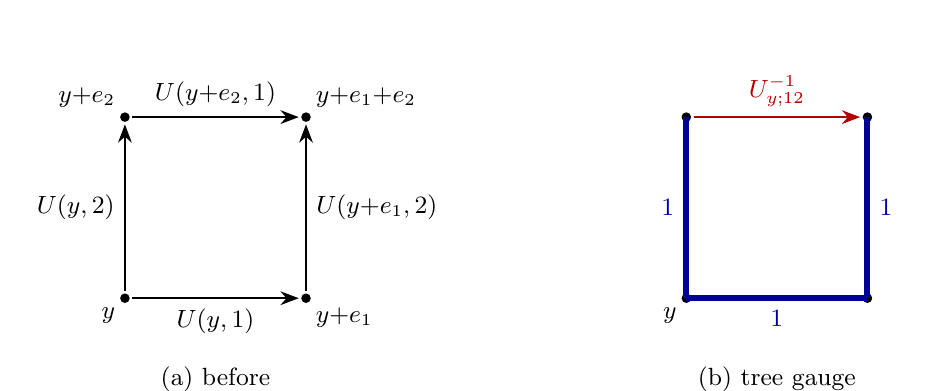
\begin{tikzpicture}[scale=1.15,>=Stealth,font=\small]
\begin{scope}
 \foreach \p/\n in {(0,0)/y,(2,0)/{y+e_1},(2,2)/{y+e_1+e_2},(0,2)/{y+e_2}}{\fill \p circle (1.5pt);}
 \node[below left] at (0,0) {$y$};
 \node[below right] at (2,0) {$y{+}e_1$};
 \node[above right] at (2,2) {$y{+}e_1{+}e_2$};
 \node[above left] at (0,2) {$y{+}e_2$};
 \draw[->,thick] (0.08,0) -- (1.92,0) node[midway,below] {$U(y,1)$};
 \draw[->,thick] (2,0.08) -- (2,1.92) node[midway,right] {$U(y{+}e_1,2)$};
 \draw[->,thick] (0,0.08) -- (0,1.92) node[midway,left] {$U(y,2)$};
 \draw[->,thick] (0.08,2) -- (1.92,2) node[midway,above] {$U(y{+}e_2,1)$};
 \node at (1,-0.9) {(a) before};
\end{scope}
\begin{scope}[xshift=6.2cm]
 \foreach \p in {(0,0),(2,0),(2,2),(0,2)}{\fill \p circle (1.5pt);}
 \node[below left] at (0,0) {$y$};
 \draw[line width=2.2pt,blue!60!black] (0,0) -- (2,0) node[midway,below] {$1$};
 \draw[line width=2.2pt,blue!60!black] (2,0) -- (2,2) node[midway,right] {$1$};
 \draw[line width=2.2pt,blue!60!black] (0,0) -- (0,2) node[midway,left] {$1$};
 \draw[->,thick,red!70!black] (0.08,2) -- (1.92,2) node[midway,above] {$U_{y;12}^{-1}$};
 \node at (1,-0.9) {(b) tree gauge};
\end{scope}
\end{tikzpicture}
\caption{Tree gauge on one plaquette. After the gauge transformation the tree links (thick) equal~$1$, and the remaining link carries the inverse of the plaquette holonomy based at the root~$y$.}\label{fig:B-tree-gauge}
\end{figure}

In each block $\ell y+\mathbb B_{(\ell-1)/2}$ fix an axial spanning tree rooted at $\ell y$, and set its tree links to~$1$. (Section~\ref{subsec:B-energy} allows every rooted block-tree gauge.) The remaining logarithmic link coordinates form the axial field~$\psi$. For a fine edge $e=(x,a)$ put
\begin{gather*}
(\operatorname{rep}V)_e=\begin{cases}
V_{(y,a)},&y=\operatorname{parent}(x),\ \operatorname{parent}(x+e_a)=y+e_a,\\
1,&\operatorname{parent}(x+e_a)=\operatorname{parent}(x),
\end{cases}\\
U(v,\psi)_e=\exp((\iota_{\rm ax}\psi)_e)(\operatorname{rep}\exp v)_e.
\end{gather*}
Here $\operatorname{dir}(e)=a$ for $e=(x,a)$, $\operatorname{parent}$ takes the centred block containing a site, $\operatorname{parent}(e)=\operatorname{parent}(x)$, and $\iota_{\rm ax}$ extends by zero on tree edges. The block-constant lift $\operatorname{rep}V$ is one on every tree edge. The fine leading action is the hypercubic average of
\begin{equation*}
\mathcal A_f(U)=c_{{\rm dir},j}\sum_\square\wilsonterm(U_\square)
 +\tfrac12\sum_{x,\mathfrak p}|\mathcal L_{\mathfrak p}^{\rm path}(U,x)|^2
 +\sum_{x,i}(\mathfrak a_i^{(3)}+\mathfrak a_i^{(4)})(U,x).
\end{equation*}
The transported curvatures and coefficients are those of Definition~\ref{def:D23}, with masks and clipping removed. The action excludes the inherited quadratic loop action and the common inverse coupling. Let $S(v,\psi)$ be this action at $U(v,\psi)$ plus
\begin{equation*}
\blockpenalty\sum_{e\ {\rm coarse}}\wilsonterm\bigl((\exp v)_eQ_e^{\rm pred}(U(v,\psi))^{-1}\bigr)\,,
\end{equation*}
again without the common inverse coupling, and put $\mathsf Q=D_\psi^2S(0,0)$. The path bounds make these unclipped sums analytic near zero.

\paragraph{Block norms.}
A fine field that is smooth on the block scale has energy of order $\mu^2\|u\|^2$, with $\mu=\ell^{-1}$, so ordinary $\ell^2$ norms would lose a factor of order~$\ell^2$ in inverse bounds. The block norm removes this loss by weighting each fine Fourier alias by $(\mu^2+|q|^2)^{1/2}$. For this finite Fourier matrix use the residue representatives $x,z\in\{0,\ldots,\ell-1\}^4$; the kernel estimates below use centred representatives instead. Put $\mu=\ell^{-1}$, $\theta_z(\xi)=(\xi+2\pi z)/\ell$, and
\begin{gather*}
\omega_z(\xi)=\bigl(\mu^2+\sum_a|q_a(\operatorname{Re}\theta_z(\xi))|^2\bigr)^{1/2},\\
\mathcal U_\ell(\xi)_{xz}=\ell^{-2}\mathrm e^{i\theta_z(\xi)\cdot x},\quad
T_\ell(\xi)=\mathcal U_\ell(\xi)\operatorname{diag}(\omega_z(\xi)^{-1})\mathcal U_\ell(0)^{-1}\,.
\end{gather*}
A fine Bloch field at coarse momentum~$\xi$ obeys $u(x+\ell n)=\mathrm e^{i\xi\cdot n}u(x)$, and $\hat u=\mathcal U_\ell(\xi)^{-1}u$ are its alias coordinates on the fixed cell. For real~$\xi$ the block norm and its dual are
\begin{equation*}
\|u\|_{\rm bl}^2=\sum_z\omega_z(\xi)^2|\hat u_z|^2,\qquad
\|f\|_{{\rm bl},*}^2=\sum_z\omega_z(\xi)^{-2}|\hat f_z|^2,
\end{equation*}
the fine $H^1$ norm with mass~$\mu$ and its dual, in Bloch coordinates; coarse coordinates carry the Euclidean norm. Since $\mathcal U_\ell(\xi)$ is unitary for real~$\xi$, $\|u\|_{\rm bl}=\|T_\ell(\xi)^{-1}u\|$; the last factor of~$T_\ell$ fixes the reference cell. On the strip $\mathcal S_\eta=\{\xi\in\C^4:|\operatorname{Im}\xi_a|<\eta\}$ we use this formula as the definition: $T_\ell$ on fine links or sites, the identity on coarse coordinates, direct sums on products, and $T_\ell(-\xi)^{-T}$ on dual fields. Axial variables inherit the norm of their slice embedding. For kernels set
\begin{equation*}
\|K\|_\eta^{\rm bl}=\sup\|T_{\rm out}(\xi_{\rm out})^{-1}K(\xi_{\rm out},\xi_{\rm in})T_{\rm in}(\xi_{\rm in})\|_{\rm op}\,,
\end{equation*}
the supremum over momenta whose indicated shifts all lie in~$\mathcal S_\eta$. Use tensor products for several inputs; field insertions are normalized coarse directions. The weights use $\operatorname{Re}\theta_z$ and need not be analytic. Write $W_{\rm ax}v=(v,D\psi(0)v)$ for the axial tangent, and retain $W_0$ for the smooth free interpolation before axial gauge. They are distinct coordinate representatives.

The next lemma supplies the stationary configuration and identifies its first derivative with the free solution. Let $\nabla_f^r$ denote any product of $r$ forward fine differences. Fix an integer $r_0\ge0$ with $r_0\le2$ or $j\ge r_0+3$, and let $x$ be any centred fine residue. The constants $c_j>0$ and $C_{j,r}$ depend on the stage and derivative order, but not on the ratio, history or period.
\begin{lemma}[Stationary interpolation]\phantomsection\label{lem:B3}
\begin{enumerate}[label=(\roman*)]
\item Near zero there is an analytic stationary branch with
\begin{equation*}
D_\psi S(v,\psi(v))=0,\quad \psi(0)=0,\quad \mathsf Q\ge\nu_{j,\ell} I\,,
\end{equation*}
where $\nu_{j,\ell}>0$ does not depend on the period.
\item $D\psi(0)$ is the axial representative of the free interpolation: $\operatorname{rep}v+\iota_{\rm ax}D\psi(0)v$ is the tree representative of~$W_0v$.
\item The averaging symbol equals one at zero and vanishes to order at least $j$ at every nonzero alias.
\item For $0\le r\le r_0$ and every bounded coarse field~$v$, the following bounds hold for $W_0=W_{\rm r}$ and, with $W_0$ replaced by $W_{\rm s}$, for the centred representative:
\begin{gather*}
|\nabla_f^rW_0(\ell y+x,y')|\le C_{j,r}\ell^{-1-r}e^{-c_j|y-y'|},\\
\|\nabla_f^rW_0v\|_\infty\le C_{j,r}\ell^{-1-r}\|v\|_\infty.
\end{gather*}
\end{enumerate}
\end{lemma}
The proof uses a local axial estimate for coercivity, a finite-dimensional implicit equation for the branch, and the alias decay of the averaging symbol for the kernel bounds.
\begin{proof}
\emph{The minimizing choices are analytic.} At the flat field the frame objective has quadratic part $\operatorname{av}_{r,r'}|h_r-h_{r'}|^2/2$. On $h_0=0$ this is positive definite. The predictor objective has Hessian~$I$ in its group variable. Their chart equations are real analytic. Their local complexifications and the analytic implicit function theorem make both minimizing choices real analytic near zero. Apply~\cite[Theorem~1.3.8]{Lebl2026} to the complexified chart equations, which vanish at zero and have the displayed invertible Hessians. The neighbourhoods may depend on the period.

For a fine infinitesimal field~$a$, let $I_a(x\to x';o)$ be its signed sum along the route. Differentiating the frame equation gives
\begin{equation*}
\tau_y(r)=-\operatorname{av}_{r',o}I_a(\ell y+r\to\ell y+r';o),\quad
h_{y,r}'=\tau_y(r)-\tau_y(0),\quad
\mathcal Q_ma=\mathcal M_ma+d_0\mathcal F_ma\,.
\end{equation*}
Here $\mathcal F_ma(y)=\tau_y(0)-\sum_rw_r^{\rm av}\tau_y(r)$. In particular $\mathcal Q_md_0\phi=d_0(\phi\circ\iota)$.

\emph{Coercivity on the axial slice.} Telescoping the boundary of each coordinate rectangle expresses a free link as a block-constant coarse-link value plus curls in its enlarged block. Averaging the straight connectors replaces the coarse-link value by~$\mathcal Q_ma$; the frame differences are route sums of the same curls. For example, interchanging two positive steps gives
\begin{equation*}
a_a(x)+a_b(x+e_a)-a_b(x)-a_a(x+e_b)=(d_1a)_{ab}(x).
\end{equation*}
Reverse steps change the sign and translate this identity. Repeated interchanges compare the tree route, a straight connector and its averaged translates. Thus, at each free edge~$e$,
\begin{equation*}
|a_e|\le C_{j,\ell}\sum_{\square\in\ell\,\operatorname{parent}(e)+\mathbb B_{(j+7)\ell}}|(d_1a)_\square|
+|(\mathcal Q_ma)_{\operatorname{parent}(e),\operatorname{dir}(e)}|\,.
\end{equation*}
This is an identity followed by a triangle inequality: tree-edge coordinates are zero, and every interchange of two successive route steps contributes exactly one signed curl. Cauchy--Schwarz and the bounded number of enlarged blocks containing a given plaquette give constants $A_{j,\ell},B_{j,\ell}<\infty$, independent of the period, with
\begin{equation*}
\|a\|_2^2\le A_{j,\ell}\|d_1a\|_2^2+B_{j,\ell}\|\mathcal Q_ma\|_2^2\,.
\end{equation*}
The row construction of Section~\ref{subsec:C-matching}, at the finer input level, identifies the leading Hessian with $\mathsf K_f=d_1^*\mathsf H_fd_1$; Lemma~\ref{lem:C2} fixes its normalization at zero momentum. Cubic and quartic curvature atoms have zero quadratic derivative. Consequently, for the slice embedding~$\iota_{\rm ax}$,
\begin{equation*}
\langle \psi,\mathsf Q\psi\rangle
=\langle d_1\iota_{\rm ax}\psi,\mathsf H_f d_1\iota_{\rm ax}\psi\rangle
+\blockpenalty\|\mathcal Q_m\iota_{\rm ax}\psi\|^2\ge\nu_{j,\ell}\|\psi\|^2\,,
\end{equation*}
with $\nu_{j,\ell}=\min(2\gamma_j,\blockpenalty)/(1+A_{j,\ell}+B_{j,\ell})$ (Lemma~\ref{lem:B2}(ii)).

\emph{The branch and its tangent.} The map $\mathcal E(v,\psi)=D_\psi S(v,\psi)$ is analytic, $\mathcal E(0,0)=0$, and $D_\psi\mathcal E(0,0)=\mathsf Q$. The same implicit function theorem gives $\psi(v)$. Differentiation yields
\begin{equation*}
D\psi(0)=-\mathsf Q^{-1}D_vD_\psi S(0,0)\,.
\end{equation*}
To identify this tangent, note that at the flat field the quadratic part of $S(v,\cdot)$ in the fine field $a=\operatorname{rep}v+\iota_{\rm ax}\psi$ is one half of $\langle a,\mathsf K_fa\rangle+\blockpenalty\|\mathcal Q_ma-v\|^2$. By the energy identity (Step~6 of the proof of Lemma~\ref{lem:B2}), $W_0v$ minimizes it over all fine fields; a gradient $d_0\phi$ with $\phi$ vanishing at the block roots changes neither term, and exactly one such modification of~$W_0v$ has zero tree links. By coercivity it is the unique minimizer over the slice, which proves~(ii). In centred coordinates $c'(a)=-\mathcal F_ma$, so the centred tangent $(W_{\rm s}v,0)$ has rooted-frame component $\mathcal F_mW_{\rm s}v$. The joint gauge transformation with parameter $I_\ell(\mathcal F_mW_{\rm s}v)$ changes this pair to $(W_{\rm r}v,0)$ at the same coarse input. Tree gauge is applied after this transformation. In particular the tree projections of the two fine fields alone need not coincide. The implicit neighbourhood may depend on the volume; the coercivity constant does not.

\emph{Kernel bounds.} First apply the alias calculation of Lemma~\ref{lem:B2} to $W_{\rm s}$; equation~\eqref{eq:B-root-centred} then gives the same fine-difference bounds for $W_0=W_{\rm r}$. Finally $\widehat w^{\rm av}(\theta)=\widehat w_\ell(\theta)^j$. At a nonzero alias $2\pi z/\ell$, at least one centred geometric sum has a simple zero, so the product has a zero of order at least~$j\ge4$. At zero it equals one. For a word of $r$ fine differences the alias multiplier is a product of $r$ factors $q_{a_h}(\theta_z)$, each bounded by $C\ell^{-1}(1+|z|)$. This includes a difference crossing a fine cell boundary: its Bloch phase shifts the coarse base and gives exactly the same multiplier. After separating the principal pole as in Lemma~\ref{lem:B2}, the interpolation alias has the bound $C_j\ell^{-1}\prod_{a=1}^4(1+|z_a|)^{-j}$ on a common smaller strip. The centred-residue exponential is bounded there. Consequently the sum of absolute alias terms after $r$ differences is at most
\begin{equation*}
C_{j,r}\ell^{-1-r}\sum_{z\in\Z^4}(1+|z|)^r
 \prod_{a=1}^4(1+|z_a|)^{-j}
\le C'_{j,r}\ell^{-1-r}\qquad(r\le j-2).
\end{equation*}
Indeed $(1+|z|)^r\le C_r\prod_a(1+|z_a|)^r$ and each remaining exponent is at least two. The pole-free principal term has the same bound. This proves the required symbol estimate through order two for $j\ge4$, and through order $r_0$ for $j\ge r_0+3$. There are finitely many difference words at a fixed stage; take a common smaller strip for them. Shifting the four coarse Fourier contours towards the sign of the displacement gives the first bound in~(iv). It includes all link components and is uniform in the centred fine residue~$x$. Summing over $y'$ proves the second bound. Periodization preserves the row bound by the triangle inequality.

The same kernel bound permits polynomially growing inputs. For $0\le c'<c_j$ and $h\ge0$ put
\begin{equation*}
w_{c',h}(y)=e^{c'|y|}(1+|y|)^h,\qquad
\|v\|_{c',h}=\sup_y\frac{|v(y)|}{w_{c',h}(y)}.
\end{equation*}
The triangle inequality gives $w_{c',h}(y')/w_{c',h}(y)\le e^{c'|y-y'|}(1+|y-y'|)^h$. Thus absolute kernel summation yields
\begin{equation}\label{eq:B-weighted-interp}
\sup_{y,x}\frac{|\nabla_f^rW_0v(\ell y+x)|}{w_{c',h}(y)}
\le C_{j,r,c',h}\ell^{-1-r}\|v\|_{c',h}.
\end{equation}
The sum converges since $c'<c_j$. In particular~\eqref{eq:B-weighted-interp} applies to polynomial jets of any fixed degree and to a cubic remainder when $j\ge6$.
\end{proof}

\paragraph{Gaussian coordinates.}
Write $U_v=U(v,\psi(v))$ and $\mathsf Q(v)=D_\psi^2S(v,\psi(v))$. Let $s$ change axial logarithmic increments to left increments at~$U_v$, and let $J_{\rm ax}$ be the product Haar density in these coordinates divided by its value at zero. For $x=\ell y+r$ in its centred block, set $\Psi(U,h_{\rm fr})(x)=h_{\rm fr}(y)h_{y,r}(U)$, using the patch frame of Definition~\ref{def:D20b}. This extends a coarse frame~$h_{\rm fr}$ over each fine block. The joint variable is $(U,h_{\rm fr})$, with gauge action
$(U,h_{\rm fr})\mapsto(U^\gamma,h_{\rm fr}(\gamma\circ\iota)^{-1})$.
Let $\mathcal R$ insert fine site gauge parameters, and let $\mathcal I$ embed free-edge increments, with zero coarse-frame component. Thus
$(\mathcal R,\mathcal I):\g^{\rm fine\ sites}\oplus\g^{\rm free\ edges}\to\g^{\rm fine\ edges}\oplus\g^{\rm coarse\ sites}$ is square: the number of tree edges is the number of fine sites minus the number of block roots. Write $\mathsf J(U,h_{\rm fr})$ for the joint left Hessian of the leading action plus block penalty, with the coarse field fixed. We evaluate it along the stationary background; its value at the flat field has fine kinetic part $\mathsf K_f$. Put
\begin{equation*}
X=D_{w=0}[-\log(\Psi(U,h_{\rm fr})^{-1}\Psi(\mathrm e^w(U,h_{\rm fr})))],\qquad
\mathcal L_{m+1}=\sum_{x,i}\mathfrak a_i^{(2)}(\,\cdot\,,x)\,.
\end{equation*}
The last sum is the inherited quadratic loop action of Definition~\ref{def:D23}. The \emph{one-loop action} is
\begin{equation*}
\mathsf T(v)=\mathcal L_{m+1}(U_v)+\tfrac12\log\det\mathsf Q(v)-\log J_{\rm ax}(v).
\end{equation*}
It is the negative logarithm of the field-dependent Gaussian factor.

The determinant and coordinate density must be compared in the same counting coordinates. Let $n$ be the number of real axial coordinates.
\begin{lemma}[Gaussian coordinates]\label{lem:B4}
Near $v=0$ the Hessian $\mathsf Q(v)$ is positive,
\begin{equation*}
J_{\rm ax}=|\det Ds|>0,\qquad J_{\rm ax}(0)=1,\qquad
X\mathcal R=I,\qquad \det(\mathcal R,\mathcal I)^2=1,
\end{equation*}
and, for every $\beta>0$,
\begin{equation*}
J_{\rm ax}(v)\,\mathrm e^{-\mathcal L_{m+1}(U_v)}\int\mathrm e^{-\frac\beta2\langle w,\mathsf Q(v)w\rangle}\,dw
=\Bigl(\frac{2\pi}\beta\Bigr)^{n/2}\mathrm e^{-\mathsf T(v)}.
\end{equation*}
Thus the stationary Gaussian integral, including the inherited loop action and the Haar density, has field-dependent factor $\mathrm e^{-\mathsf T(v)}$.
\end{lemma}
The proof computes the Haar density in axial coordinates at the stationary point. Lemma~\ref{lem:C5} then rewrites the determinant in gauge-completed form; \eqref{eq:B-one-loop-box} below collects the resulting normalization.
\begin{proof}
Tree gauge is an exact Haar change of variables. In tree order, each tree link is a Haar translate of its child gauge variable, whose integral is one. For fixed $V$, gauge transformations fixing every block root leave the kernel of Definition~\ref{def:D04} invariant. Integration of these gauge variables reduces its integral to product Haar measure on free links; root transformations are not integrated here. In exponential coordinates write this measure as $J_*^{n_e}\prod_eJ(\psi_e)\,d\psi$, with $J(0)=1$ and $n_e$ the number of free links.

At a fixed stationary axial point~$y=\psi(v)$ the coordinate change on each free link is
\begin{equation*}
s_y(\psi)_e=\log(\exp \psi_e\exp(-y_e)),\qquad s_y(y)=0\,.
\end{equation*}
Right invariance of Haar measure gives $\prod_eJ(\psi_e)=|\det Ds_y(\psi)|\prod_eJ(s_y(\psi)_e)$. Evaluate at~$\psi=y$ to obtain $J_{\rm ax}(v)=|\det Ds_y(y)|$. Since $Ds_0(0)=I$, its value at zero is one, and it stays positive nearby. Stationarity removes the second-derivative term in the Hessian chain rule, giving
\begin{equation}\label{eq:B-hessian-chain}
\mathsf Q(v)=(Ds)^*(\mathcal I^*\mathsf J\mathcal I)Ds
\end{equation}
for the joint left Hessian~$\mathsf J$.

Gauge covariance of~$\Psi$ gives $X\mathcal R=I$. In tree-height order, each tree-edge row of~$(\mathcal R,\mathcal I)$ has its child gauge coordinate~$\pm I$ and earlier gauge coordinates; each coarse-frame row has its root gauge coordinate $-I$, and every free-edge slice column has its identity entry. Thus $\det(\mathcal R,\mathcal I)^2=1$. Positivity of $\mathsf Q(0)$ from Lemma~\ref{lem:B3} persists near zero.

The Gaussian integral of the positive form $\frac\beta2\langle w,\mathsf Q(v)w\rangle$ equals $(2\pi/\beta)^{n/2}(\det\mathsf Q(v))^{-1/2}$. Multiplying by $J_{\rm ax}(v)\mathrm e^{-\mathcal L_{m+1}(U_v)}$ gives the displayed identity by the definition of~$\mathsf T$. The factors $J_*^{n_e}$ and $(2\pi/\beta)^{n/2}$ do not depend on~$v$; they enter the scalar normalization.
\end{proof}

\subsection{Inverse, vertex and Ward estimates}\label{subsec:B-inverse}

Section~\ref{sec:partII-C} extracts the curvature-square coefficient of~$\mathsf T$ by comparing it with an auxiliary fine determinant. This subsection supplies three inputs for that comparison: inverse bounds uniform in the block ratio (Lemma~\ref{lem:B7}), vertex bounds (Lemma~\ref{lem:B5}), and a Ward identity for the predictor contact term (Lemma~\ref{lem:B6}).

\paragraph{The regulator.} For a fine site field put
\begin{equation*}
(d_U\phi)_e=\phi(e^-)-\operatorname{Ad}(U_e)\phi(e^+),\quad
\Delta_U=d_U^*d_U,\quad P_\mu=\mu^2(\Delta_U+\mu^2I)^{-1},\quad
\mathfrak m_\mu=\mu^2P_\mu^9\,,
\end{equation*}
with $\mu=\ell^{-1}$. The regulator $\mathfrak m_\mu$ acts as a mass at the block scale: by~\eqref{eq:B-mass-floor} below, $\Delta_0+\mathfrak m_\mu\ge2^{-10}(\Delta_0+\mu^2)$, so below momentum~$\mu$ it is a mass of order~$\mu^2$, while above~$\mu$ it decays like $\mu^2(\mu/|k|)^{18}$. The ninth power is chosen because $P_\mu^3$ is trace class at each coarse momentum, uniformly in~$\ell$ (Lemma~\ref{lem:B7}(i)). After two field derivatives of $\mathfrak m_\mu=\mu^2(P_\mu^3)^3$ one undifferentiated factor $P_\mu^3$ remains, and its trace norm keeps the $\ell^4$ fine aliases out of the determinant comparison.

\paragraph{The predictor contact term.} At the stationary background for~$v$, let $Q_v(w)$ be the framed predictor in left increments~$w$ of the joint fine-link and frame variables. Set $Q_0(v)=Q_v(0)$ and use the output chart based at this predictor:
\begin{equation*}
p_v(w)=\log\bigl(Q_v(w)Q_0(v)^{-1}\bigr),\qquad
\mathrm{Pen}_v(p)=\blockpenalty\sum_e\wilsonterm\bigl((\exp v)_e(\exp p_e\,Q_{0,e}(v))^{-1}\bigr).
\end{equation*}
The base $Q_0(v)$ is held fixed when differentiating in~$w$; derivatives in~$v$ also differentiate this base. In these coordinates the penalty is unchanged. The second-derivative chain rule at $w=0$ gives
\begin{equation}\label{eq:B-contact}
\begin{aligned}
D_w^2(\mathrm{Pen}_v\circ p_v)&=H^*BH+\sum_\lambda d^\lambda C_\lambda,\\
H&=D_wp_v,\quad B=D_p^2\mathrm{Pen}_v(0),\quad
d=D_p\mathrm{Pen}_v(0),\quad C_\lambda=D^2_w(p_v)_\lambda .
\end{aligned}
\end{equation}
The index $\lambda$ comprises a coarse link and a colour index. The last sum is the \emph{predictor contact term}; this use of the word is unrelated to the contact extensions of Theorem~\ref{prop:CT}. The internal derivatives defining $H$ and $C_\lambda$ use the rooted left increments. In centred fibres their tensors and $\mathsf C_\mu^{\rm rem}$ are pulled back by the same triangular tangent at each background. In particular, $C_\lambda$ is not replaced by the raw second derivative in a nonlinear centred chart. Along the stationary field, $d(0)=0$ and $Dd(0)=-\mathsf K_c$: at zero the based and absolute output charts have the same first derivative, and the normal equation gives $\blockpenalty(I-\mathcal Q_mW_0)=\mathsf K_c$ (Step~6 of the proof of Lemma~\ref{lem:B2}).

\paragraph{The compared operators.} The gauge-completed Hessian, the ghost operator and the auxiliary fine operator are
\begin{equation*}
\mathsf C_\mu=\mathsf J+F_\mu^*F_\mu,\quad F_\mu=d_U^*P_f+\mathfrak m_\mu X,\qquad
\mathsf G_\mu=\Delta_U+\mathfrak m_\mu,\qquad
\mathsf A^{\rm aux}_\mu=\mathsf A+d_Ud_U^*+\mathsf M_\mu ,
\end{equation*}
where $P_f$ projects to fine links, $\mathsf A(U)$ is the fine leading Hessian and $\mathsf M_\mu$ applies $\mathfrak m_\mu$ to each link component. Frame covariance gives $F_\mu\mathcal R=\mathsf G_\mu$. Write $\mathsf C^{\rm rem}_\mu$ for $\mathsf C_\mu$ with the contact term of~\eqref{eq:B-contact} removed; at the flat field $\mathsf C^{\rm rem}_\mu=\mathsf C_\mu$, since $d(0)=0$.

These operators give the one-loop action a single normalization. The second line below follows from~\eqref{eq:B-hessian-chain} and $J_{\rm ax}=|\det Ds|$, the third from Lemma~\ref{lem:C5}. For every $\mu>0$ and $v$ in a neighbourhood of zero,
\begin{equation}\label{eq:B-one-loop-box}
\boxed{\begin{aligned}
\mathsf T(v)&=\mathcal L_{m+1}(U_v)+\tfrac12\log\det\mathsf Q(v)-\log J_{\rm ax}(v)\\
&=\mathcal L_{m+1}(U_v)+\tfrac12\log\det(\mathcal I^*\mathsf J(v)\mathcal I)\\
&=\mathcal L_{m+1}(U_v)+\tfrac12\log\det\mathsf C_\mu(v)-\log\det\mathsf G_\mu(v).
\end{aligned}}
\end{equation}
The factor $\tfrac12$ comes from the Gaussian integral; the Haar Jacobian converts the axial Hessian to left coordinates: $\det\mathsf Q=J_{\rm ax}^2\det(\mathcal I^*\mathsf J\mathcal I)$; the ghost determinant enters with power one because the gauge block of the completion contributes $(\det\mathsf G_\mu)^2$ to $\det\mathsf C_\mu$. The left side does not depend on~$\mu$. Field-independent factors, such as $(2\pi/\beta)^{n/2}$ and the Haar normalizations, form the scalar normalization; they cancel from every normalized expectation, so the convergence of correlations does not require them to converge. Only the dependence of~$\mathsf T$ on~$v$ matters for correlations: Section~\ref{sec:partII-C} extracts the coupling coefficient from its quadratic kernel, and its higher Taylor terms enter the activities of Section~\ref{sec:partII-D}.

\paragraph{Insertion bounds.} For weighted bounds use the nearest projection~$\pi$ from Lemma~\ref{lem:B1} and centred coarse frames: $c_y(U)=\pi(\sum_r w_r^{\rm av}h_{y,r}(U))$, $\widetilde h_{\rm fr}=h_{\rm fr}c(U)$. Pull back the joint quadratic forms by this change. Its tangent is triangular with identity diagonal, so it preserves determinants. Lemma~\ref{lem:C6} compares $\mathsf C^{\rm rem}_\mu$ with $\mathsf A^{\rm aux}_\mu$; derivatives are at zero in free interpolated coarse directions. Let $A_\mu$ denote either of these two operators. Its smooth centred background insertions use the joint direction $(v,W_{\rm s}v,0)$.

The uninserted inverse and the geometric insertions are controlled by one constant~$C_j^{\rm ins}$, chosen before the nonlinear path bounds; the derivatives of the full Hessian also contain the input path coefficients. For $r=1,2$ let $M_r$ be the supremum of $\|D^rA_\mu\|$ from the primal block space to its dual, in normalized smooth coarse directions, on any common smaller strip for these inserted kernels. Define
\begin{equation*}
\mathcal P^{\rm inv}_0(C)=C,\qquad \mathcal P^{\rm inv}_1(C)=C^2M_1,\qquad
\mathcal P^{\rm inv}_2(C)=2C^3M_1^2+C^2M_2.
\end{equation*}
The norms $M_1,M_2$ retain the actual cubic and quartic path contributions. The proof of the next lemma also shows, on a smaller common strip,
\begin{equation}\label{eq:B-Mr}
\sup_\ell M_r\le\mathcal P_{j,r}(A_j^{\rm path}),\qquad r=1,2,
\end{equation}
where $A_j^{\rm path}$ is the stage path bound of item~4 of Table~\ref{tab:constant-choices}; the fixed polynomials also depend on the interpolation, free metric, frame and penalty bounds.

These estimates control the determinant comparison without a factor equal to the number of fine sites. The inserted-kernel bounds in parts (i)--(iii) require the common ratio-uniform shifted-strip estimate identified as unresolved in Step~5 of the proof.
\begin{lemma}[Scaled inverse insertions]\label{lem:B7}
There are $\eta_j^{\rm inv}>0$ and $C_j^{\rm ins}<\infty$, fixed before the ratio and path bounds, such that for $A_\mu\in\{\mathsf C^{\rm rem}_\mu,\mathsf A^{\rm aux}_\mu\}$, $0\le r\le2$ and every odd $\ell$ allowed by item~5 of Table~\ref{tab:constant-choices}:
\begin{enumerate}[label=(\roman*)]
\item $\sup_{\xi\in\mathcal S_{\eta_j^{\rm inv}}}\|P_\mu(\xi)^3\|_1\le C_j^{\rm ins}$ and $\|D^rP_\mu\|_{\eta_j^{\rm inv}}^{\rm bl}\le C_j^{\rm ins}$;
\item $\|D^r(A_\mu^{-1})\|_{\rm dual\to primal}\le\mathcal P^{\rm inv}_r(C_j^{\rm ins})$ and $\|\mu^2D^r(A_\mu^{-1})\|^{\rm bl}\le\mathcal P^{\rm inv}_r(C_j^{\rm ins})$;
\item on the common smaller strip, block-penalty and frame insertions have norms at most $C_j^{\rm ins}$.
\end{enumerate}
\end{lemma}
We first prove real coercivity in block units, then extend it to a strip and differentiate the inverse. Constants depend on the free bounds of Lemma~\ref{lem:B2}, the stage and~$\blockpenalty$.
\begin{proof}
\emph{Step 1: the mass floor.} At zero background, $\Delta_0$ has symbol~$\lambda(\theta)$. With $x=\lambda(\theta)\ge0$,
\begin{equation}\label{eq:B-mass-floor}
2^{-10}(x+\mu^2)\le x+\mu^2\left(\frac{\mu^2}{x+\mu^2}\right)^9\le x+\mu^2\,.
\end{equation}
For $x\ge\mu^2$ the first term supplies the lower bound; for $x<\mu^2$ the parenthesis is at least~$1/2$. On links, the exterior identity $\|d_1u\|^2+\|d_0^*u\|^2=\lambda(\theta)\|u\|^2$ and Lemma~\ref{lem:B2} give the same lower bound, with a fixed positive factor, for the auxiliary fine operator. Changing its quadratic form by~$T_\ell$ therefore gives a positive lower bound independent of~$\ell$.

\emph{Step 2: coercivity modulo gauge.} In centred coordinates fine gauge insertion has coarse component $-\sum_r w_r^{\rm av}\phi(\ell y+r)$: differentiate $h_{y,r}(U^\gamma)=\gamma(\ell y)h_{y,r}(U)\gamma(\ell y+r)^{-1}$ and the centroid. The uncompleted joint form is
\begin{equation*}
\langle d_1u,\mathsf H_fd_1u\rangle+\blockpenalty\|\mathcal M_mu-d_0\vartheta\|^2\,.
\end{equation*}
Modulo a joint gauge transformation choose $\vartheta=0$ and make every nonprincipal fine alias transverse. This is possible by dividing its longitudinal part by~$\lambda(\theta_z)$; the remaining principal gauge parameter fixes~$\vartheta$, since the principal averaging multiplier is bounded below by~\eqref{eq:B-filter}. Write $u_z$ for the resulting normalized alias coordinates and $H_>=\sum_{z\ne0}\omega_z^2|u_z|^2$. The fine curvature energy bounds $cH_>$. The averaging multiplier on the principal alias is at least $c_j\mu$ in unitary cell coordinates; the weighted norm of all other alias columns is at most~$C_j$. Therefore
\begin{equation*}
(c_j\mu|u_0|)^2\le2\|\mathcal M_mu\|^2+2C_j^2H_>,\qquad \omega_0\le C\mu\,.
\end{equation*}
Combining these inequalities shows that the uncompleted form at~$w$ is at least $c\operatorname{dist}_{\rm bl}(w,\operatorname{ran}\mathcal R)^2$, with $c$ independent of~$\ell$.

\emph{Step 3: gauge completion.} Let $\mathcal R\phi$ be joint gauge insertion. Frame covariance gives $F_\mu\mathcal R=\Delta_0+\mathfrak m_\mu$ at zero background. By~\eqref{eq:B-mass-floor},
\begin{equation*}
\|\mathcal R\phi\|_{\rm bl}\le C\|(\Delta_0+\mathfrak m_\mu)\phi\|_2,\qquad
\|F_\mu w\|_2\le C\|w\|_{\rm bl}\,.
\end{equation*}
For the second bound one must also estimate $\mathfrak m_\mu X$ on arbitrary fine increments. In the centred frame, $X$ is a sum of normalized averages of routes of length at most $C_j\ell$. Its row and column sums are at most $C_j\ell$, so
\begin{equation*}
\|Xu\|_2\le C_j\ell\|u\|_2\le C_j\mu^{-2}\|u\|_{\rm bl},\qquad
\|\mathfrak m_\mu X u\|_2\le C_j\|u\|_{\rm bl}.
\end{equation*}
The coarse-frame part satisfies the same inequality since its embedding has $\ell^2$ as counting-norm factor and $\|\mathfrak m_\mu\|\le\mu^2$. Also $\|d_0^*u\|_2\le C\|u\|_{\rm bl}$. For the first bound a fine gauge component contributes $\omega_z|q(\theta_z)\phi_z|\le \omega_z^2|\phi_z|$, and its averaged coarse component is bounded by the summable alias filter times~$\omega_z^2|\phi_z|$. For $w=w_\perp+\mathcal R\phi$, the completed energy bounds $c\|w_\perp\|_{\rm bl}^2+\|F_\mu w\|_2^2$. The last two inequalities give
\begin{equation*}
\|w\|_{\rm bl}\le\|w_\perp\|_{\rm bl}+C\bigl(\|F_\mu w\|_2+C\|w_\perp\|_{\rm bl}\bigr)\,.
\end{equation*}
Squaring proves real coercivity of the completed form with a constant independent of~$\ell$.

\emph{Step 4: the complex strip.} The uninserted quadratic symbols and the geometric frame and penalty kernels have bounded weighted norms on a fixed coarse strip. To verify this, each fine derivative is bounded by~$C\omega_z$, a free interpolated field by~$C\mu$, and normalized frame or predictor averages by the summable filter~\eqref{eq:B-filter}. At the flat field these operators depend only on the free quadratic action, the interpolation, the frame and the penalty. Their defining inserted kernels use the smooth interpolation; its fine differences of order $s\le2$ are $O(\ell^{-1-s})$ by the alias estimate~\eqref{eq:B-filter}. For complex momenta, freeze the weights at a real momentum: if the coarse displacement has norm at most one, the geometric-sum formula and $|q(\theta_z(\xi))-q(\theta_z(\xi'))|\le C\mu|\xi-\xi'|$ make the two weights comparable by a fixed factor. Cauchy's estimate~\cite[Proposition~1.2.2]{Lebl2026} on a smaller disc bounds the change of the conjugated symbol by~$C\eta$. Choose~$\eta_j^{\rm inv}$ so this is less than half the real lower bound. A Neumann series gives the weighted inverse on that strip.

\emph{Step 5: insertions.} For inserted directions $v,w$, write $A_v=DA_\mu[v]$ and $\mathsf R=A_\mu^{-1}$. Direct differentiation gives
\begin{equation*}
D\mathsf R[v]=-\mathsf RA_v\mathsf R,\qquad D^2\mathsf R[v,w]=\mathsf RA_v\mathsf RA_w\mathsf R+\mathsf RA_w\mathsf RA_v\mathsf R-\mathsf RD^2A_\mu[v,w]\mathsf R\,.
\end{equation*}
The geometric insertions have norm at most $C$: each smooth field is $O(\mu)$, each derivative on it is $O(\mu^2)$, and $\mu\le\omega_z$. With two arbitrary fine legs, Cauchy--Schwarz accounts for their two factors $\omega_z^{-1}$; a difference on either leg supplies its corresponding $\omega_z$. This bounds the block penalty, frame and $\Delta_U$ insertions independently of the nonlinear path coefficients. For the based predictor chart, external derivatives also act on $Q_0(v)$. Its derivatives are controlled by the same normalized predictor and smooth interpolation bounds; the smooth multiplication and logarithm contribute bounded geometric factors on a smaller chart. In every derivative of $H^*BH$ the intermediate space remains the coarse-link space. For the path contribution, expand each transported curvature through total degree four. Its third derivative has one curl and its fourth has zero or more differences after two smooth insertions. In either case two arbitrary fine legs contribute at most $\mu^{-2}$, while the two smooth insertions in the fourth derivative contribute $\mu^2$. For the third derivative a smooth insertion and the remaining curl give the same bound. Summation by parts moves a difference off a smooth leg when necessary; its path-length loss is summable against the exponential path bound. Each coefficient is a product of at most two path-row coefficients, or one atom coefficient. The row and atom sums therefore give a fixed polynomial $\mathcal P_{j,r}(A_j^{\rm path})$, uniformly in $\ell$. Adding the geometric insertions proves~\eqref{eq:B-Mr}. The inverse identities therefore give dual-to-primal norms $C^2M_1$ and $2C^3M_1^2+C^2M_2$. The inclusion of a primal source in the dual space has norm at most $C\mu^{-2}$; include its fixed factor in $C_j^{\rm ins}$. Multiplication by $\mu^2$ gives precisely $\mathcal P^{\rm inv}_1,\mathcal P^{\rm inv}_2$. Applying the same identities to $\Delta_U+\mu^2I$, with the geometric insertion bounds, gives the stated bounds for $D^rP_\mu$. No derivative of a weight is taken.

\emph{Unresolved inserted-kernel bound.} This step still requires a proof that the full differentiated frame and predictor kernels, with all shifted momenta, satisfy the asserted bounds on one coarse strip independent of~$\ell$ in the stated primal and dual block norms. Normalized real-space averages and the algebraic inverse identities alone do not establish that complex-strip bound. The insertion estimates in this lemma, the vertex bounds below and the determinant comparison of Lemma~\ref{lem:C6} remain conditional on it; the reflected finite-torus and local-expansion uses in Sections~\ref{sec:partII-C}--\ref{sec:partII-D} also depend on the same supplier.

\emph{Step 6: the trace bound.} In centred alias representatives,
\begin{equation*}
\left|\frac{\mu^2}{\lambda(\theta_z(\xi))+\mu^2}\right|\le C(1+|z|^2)^{-1}\,.
\end{equation*}
For real~$\xi$ this follows from $|q(k)|\ge2|k|_\infty/\pi$ on the fine momentum cube and $|\xi+2\pi z|_\infty\ge\pi|z|_\infty$ for centred aliases and $\xi\in[-\pi,\pi]^4$. The complex denominator differs from its real value by a small multiple of~$\omega_z^2$, and the Bloch Fourier matrices have bounded norms. Hence
\begin{equation*}
\|P_\mu^3\|_1\le C\dimG\sum_{z\in\Z^4}(1+|z|^2)^{-3}<\infty\,.
\end{equation*}
In $P_\mu^9=(P_\mu^3)^3$, two insertions leave one undifferentiated cube, whose trace norm bounds the regulator products; the remaining factors have bounded operator norms.
\end{proof}
The inverse is thus bounded in block units with a constant that sees neither the ratio nor the nonlinear path coefficients; these enter only through the insertion norms $M_1,M_2$.

\paragraph{Vertices.} For a translation-invariant Taylor kernel, momentum order at least~$s$ means that every coefficient of total momentum degree less than~$s$ vanishes at zero. Let $V_r$ be the degree-$r$ Taylor kernel of the fine leading action minus Wilson, for $r=2,3,4$. We use:
\begin{enumerate}[label=(\alph*)]
\item smooth free directions $\mathcal Wv=(v,W_{\rm s}v,0)$ in the coarse-link, fine-link and centred coarse-frame variables;
\item the joint action
\begin{equation*}
\mathcal S(v,u,\vartheta)=\mathcal A_f(\mathrm e^u)+\blockpenalty\sum_e\wilsonterm\left((\exp v)_e\left[Q^{\rm pred}(\mathrm e^u)^{h_{\rm fr}}\right]_e^{-1}\right),\qquad
h_{\rm fr}=\exp\vartheta\,c(\mathrm e^u)^{-1},
\end{equation*}
where the superscript is the coarse gauge action and $c$ is the centring map above, and its third and fourth derivatives $\mathcal V_3,\mathcal V_4$ at zero;
\item the vertex bounds $C_3,C_4$: the suprema on a smaller strip $\mathcal S_\eta$ of the absolute scalar Fourier entries of $\mathcal V_3,\mathcal V_4$ on momentum-conserving tuples whose legs are all $\mathcal Wv_i$ with $|v_i|\le1$, or normalized coarse legs and one fine leg of block norm at most one; these include the predictor and frame derivatives;
\item $S_{\rm stat}(v)=S(v,\psi(v))$, and, for two mixed cubic functionals annihilating joint gauge directions,
\begin{equation*}
b_h=\mathcal V_3[\mathcal Wv_{h,1},\mathcal Wv_{h,2},\cdot],\qquad h=1,2,
\end{equation*}
with axial restrictions $b_{1,\rm ax},b_{2,\rm ax}$.
\end{enumerate}
These pairings express the stationary fourth derivative in smooth coordinates. The constants $a_3,c_4$ below depend only on preceding stage data; $a_3^\prime,c_4^\prime$ may also depend on the input path bound. Put $E_{\rm ins}=\max(1,C_j^{\rm ins})$ with the constant of Lemma~\ref{lem:B7}.

The extra momentum order of the difference makes the classical matching bounds independent of the input amplitude after enlarging~$\ell$. The shifted-strip portion of these vertex bounds also requires the unresolved inserted-kernel estimate identified in the proof.
\begin{lemma}[Vertex bounds]\phantomsection\label{lem:B5}
\begin{enumerate}[label=(\roman*)]
\item The kernels $V_2,V_3,V_4$ have momentum orders at least $3,2,1$.
\item There is $u_j\ge\max(a_3',c_4')$, depending on the input path data, such that for $\ell\ge u_j$
\begin{equation*}
C_3\le a_3+\ell^{-1}a_3'\le a_3+1,\qquad C_4\le c_4+\ell^{-1}c_4'\le c_4+1\,.
\end{equation*}
\item In normalized coarse directions, $|D^4S_{\rm stat}|\le C_4+3C_3^2E_{\rm ins}$.
\item Gauge-annihilating mixed functionals satisfy $b_1\mathsf C_\mu^{-1}b_2=b_{1,\rm ax}\mathsf Q^{-1}b_{2,\rm ax}$, with $\mathsf C_\mu$ at the flat field.
\end{enumerate}
\end{lemma}
We first prove the low-momentum cancellations, using the input arrays of Lemmas~\ref{lem:C1}--\ref{lem:C2}, then count powers under the interpolation of Lemma~\ref{lem:B3}, and finally pair the cubic vertices through the completed inverse.
\begin{proof}
\emph{Momentum orders.} The quadratic difference is
\begin{equation*}
\widehat V_2(p)=\tfrac12\widehat d_1(-p)^T(\widehat{\mathsf H}_f(p)-I)\widehat d_1(p)\,.
\end{equation*}
Its middle factor vanishes at zero and its two curls each supply one momentum, proving order three.

To include the nonlinear transport terms, expand a connection with connection components of weight one and coordinate derivatives of weight one. A plaquette curvature starts at weight two, with leading term $\partial_a A_b-\partial_b A_a+[A_a,A_b]$. Changing its transport path changes this term only at higher weight. The row part at weight four is therefore its curvature square with coefficient~$c_{\rm dir}\delta_{\gamma\delta}+\sum_\alpha s_{\alpha\gamma}s_{\alpha\delta}=\delta_{\gamma\delta}$ by Lemma~\ref{lem:C2} at the finer input level; $s_{\alpha\gamma}$ are the path-row coefficients of Definition~\ref{def:D22}. Cubic and quartic curvature atoms start at weights six and eight. The Wilson action has the same weight-four term. All contributions of weight at most four consequently cancel in their difference. Polynomial connection jets vary independently. Expand their finite parallel transports through weight four and sum using the exponential path bound. A degree-$r$ field term of weight at least five has at least $5-r$ coordinate derivatives, equivalently that many momentum powers. This proves the three claimed orders, including cubic and quartic terms arising inside a quadratic curvature row.

\emph{Power counting.} An analytic coefficient $f$ vanishing at zero factors as
\begin{equation*}
f(p)=\sum_ap_a\int_0^1\partial_af(tp)\,dt\,.
\end{equation*}
Apply this to the vanishing Taylor coefficients, successively, on a smaller strip. Equivalently in position space, write $\mathrm e^{ip\cdot x}-1$ as a sum of coordinate differences; the losses are fixed powers of the true path length. The exponential path norm bounds their sums. Wilson's degrees $r=2,3,4$ have orders $4-r$; the differences have orders $5-r$.

Use the fine-difference bound for $W_0$ of Lemma~\ref{lem:B3}. For one arbitrary fine leg use Cauchy--Schwarz over the block. If it carries $s=0$ or $1$ differences, its sum of absolute values over the block is at most $C\ell^{3-s}\|u\|_{\rm bl}$: there are $\ell^4$ sites, $\|u\|_2\le\mu^{-1}\|u\|_{\rm bl}$, and $\|\nabla_fu\|_2\le C\|u\|_{\rm bl}$. Pair this with the other bounded legs. Summation by parts places at most one difference on the arbitrary leg. This gives the same bound in the dual weighted norm for a mixed vertex.

There are $\ell^4$ sites per block. A term with $r$ fields and $s$ fine differences thus has scale $\ell^{4-r-s}$. Wilson gives scale~$1$ at its leading orders, and the differences give~$\ell^{-1}$. The penalty has a fixed bound: normalized route and offset averages have mass one, straight sums cancel the factor~$\ell^{-1}$ in a smooth input, and implicit differentiation of the centred frame and predictor equations bounds their derivatives through order four. In centroid-normalized frame variables the linear equation is identity minus the constant projection; every remaining term is a normalized average, so these bounds have no factor counting patch sites. These contributions define $a_3,c_4$; the path-dependent sums define $a_3',c_4'$. Choose $u_j\ge\max(a_3',c_4')$, so that $\ell^{-1}\max(a_3',c_4')\le1$ for $\ell\ge u_j$. This gives~(ii), independently of the input path bound.

The shifted-strip bound for those differentiated frame and predictor kernels is the unresolved input identified in Step~5 of the proof of Lemma~\ref{lem:B7}. The real-space power count above does not by itself prove the common ratio-uniform complex strip required in~(ii) or its subsequent use in Section~\ref{sec:partII-C}.

\emph{The exchange term.} In the joint coordinates, the exact nonlinear tree gauge change and the stationary chain rule give
\begin{equation*}
D^4S_{\rm stat}=\mathcal V_4[\mathcal W^4]
 -\sum_{\text{three pairings}}\mathcal V_3[\mathcal W,\mathcal W,\cdot]\,
 \mathsf C_\mu^{-1}\,\mathcal V_3[\cdot,\mathcal W,\mathcal W].
\end{equation*}
Lemma~\ref{lem:B3}(ii) identifies the axial tangent with the tree representative of $W_{\rm r}$. The joint transformation described there carries the centred tangent $(v,W_{\rm s}v,0)$ to that rooted representative, including its coarse-frame component. A joint gauge transformation of the axial stationary curve remains stationary and can be chosen with tangent $\mathcal Wv$. Differentiating this curve gives the displayed formula for~$D^4S_{\rm stat}$. Each paired functional annihilates the infinitesimal gauge directions by differentiated stationarity and gauge invariance. It may therefore be paired through the completed inverse of Lemma~\ref{lem:B7}. If $b\mathcal R=0$, the shift $x\mapsto x-\mathcal R(F_\mu\mathcal R)^{-1}F_\mu x$ sets $F_\mu x$ to zero and preserves both the uncompleted energy and $b(x)$. Thus its pairing through the completed inverse equals its pairing through the slice inverse, which proves~(iv). Lemma~\ref{lem:B7} gives the constant~$E_{\rm ins}$ independently of~$\ell$ and the input path bound. Duality then bounds each pairing by $C_3^2E_{\rm ins}$. The three pairings in a symmetric fourth derivative have identical bounds. This proves~(iii).
\end{proof}

\paragraph{The stationary Ward identity.} On the smooth interpolated field write $\mathsf C^{\rm rem}_\mu(v)$ for the contact-removed completed Hessian, and let $d(v)$ and $C_\lambda(v)$ be the factors of~\eqref{eq:B-contact} there. Thus the full Hessian differs from $\mathsf C^{\rm rem}_\mu(v)$ by $\sum_\lambda d^\lambda(v)C_\lambda(v)$. To keep the derivatives of the contact insertion as well as those of the inverse, introduce an independent coarse link source $u$ and put
\begin{equation*}
\mathsf R(v,u)=\mathsf C^{\rm rem}_\mu(v)^{-1}\sum_\lambda u^\lambda C_\lambda(v),\qquad
\mathsf F(v,u)=\tr\mathsf R(v,u),\qquad
\mathsf F_2(v,u)=\tr\mathsf R(v,u)^2.
\end{equation*}
The traces sum colour and cell coordinates. Their translation-invariant kernels, with internal momentum integrated using $d\theta/(2\pi)^4$, are
\begin{equation*}
\mathsf b_{i\lambda}=\partial_{v_i}\partial_{u_\lambda}\mathsf F(0,0),\qquad
\mathsf c_{\lambda\rho}=\partial_{u_\lambda}\partial_{u_\rho}\mathsf F_2(0,0).
\end{equation*}
In particular $\mathsf c_{\lambda\rho}$ includes the two product-rule terms. Put $\mathsf a_i(\xi)=-\mathsf K_c(\xi)e_i$. Let $H^{\rm con}$ be the Hessian kernel of one half of the full minus contact-removed logarithmic determinant, evaluated on the stationary branch. Its quadratic Taylor kernel is $Y^{\rm con}=\tfrac12H^{\rm con}$.

The coefficient to be preserved is read off by
\begin{equation*}
[t^2]g(t)=\tfrac12g''(0),\qquad\alpha_b(Y)=2\operatorname{Re}[t^2]\,Y_{(2,b),(2,b)}(te_1),
\end{equation*}
for a quadratic Taylor kernel~$Y$, including the factor $1/2!$, and a colour index~$b$. The Wilson kinetic form $\frac12\langle d_1a,d_1a\rangle$ has entry $\frac12|q_1(t)|^2=\frac12t^2+O(t^4)$, hence $\alpha_b=1$; thus $\alpha_b(Y)$ is the multiple of the curvature square that $Y$ carries along transverse plane waves of small momentum. Section~\ref{sec:partII-C} uses $\alpha_b$ to define the one-loop coefficient. The cancellation below is exactly the one needed in Lemma~\ref{lem:C6}.
\begin{lemma}[Stationary Ward estimates]\label{lem:B6}
The first penalty derivative has momentum order two; $\mathsf b$ vanishes at zero and $\mathsf c$ is analytic there. For a fixed colour~$b$ and the transverse link index $i=(2,b)$,
\begin{equation*}
Y^{\rm con}_{ii}(te_1)=O(t^3),\qquad \alpha_b(Y^{\rm con})=0.
\end{equation*}
\end{lemma}
The proof derives the trace contraction from the determinant expansion and then applies the stationary gauge identity, through the tangent identification of Lemma~\ref{lem:B3}, to the mixed kernel.
\begin{proof}
The free normal equation gives $\blockpenalty(I-\mathcal Q_mW_0)=\mathsf K_c$. Hence the first penalty derivative is $\mathsf a=-\mathsf K_c$, of order two because $\mathsf K_c=d_1^*\mathsf H_cd_1$.

The determinant difference along the stationary curve is
\begin{equation*}
\tfrac12\log\det(I+\mathsf R(v,d(v)))
=\tfrac12\mathsf F(v,d(v))-\tfrac14\mathsf F_2(v,d(v))+O(|v|^3).
\end{equation*}
The first derivatives of each invariant scalar determinant vanish at the flat field: each is an adjoint-invariant linear functional on $\g$, hence zero because $\g=[\g,\g]$. In particular $\partial_u\mathsf F(0,0)=0$, so the chain-rule term $\partial_u\mathsf F(0,0)\,D^2d(0)[v,w]$ vanishes and the Hessian along the stationary curve equals that along its tangent. Since $\mathsf F$ is linear in $u$, its pure $v$ and pure $u$ Hessians vanish at $(0,0)$. The mixed derivative retains both contributions
\begin{equation*}
\partial_{v_i}\tr(\mathsf C^{\rm rem}_\mu{}^{-1}C_\lambda)
=\tr\bigl(-\mathsf C^{\rm rem}_\mu{}^{-1}(\partial_{v_i}\mathsf C^{\rm rem}_\mu)\mathsf C^{\rm rem}_\mu{}^{-1}C_\lambda
       +\mathsf C^{\rm rem}_\mu{}^{-1}\partial_{v_i}C_\lambda\bigr).
\end{equation*}
The two mixed chain-rule terms of $\mathsf F$ and the pure $u$ Hessian of $\mathsf F_2$ now give
\begin{gather*}
H^{\rm con}_{ii}(\xi)=\tfrac12\{W_i(\xi)+W_i(-\xi)-\tfrac12 V_i(\xi)\},\\
W_i(\xi)=\sum_\lambda\mathsf a_i^\lambda(\xi)\mathsf b_{i\lambda}(\xi),\qquad
V_i(\xi)=\sum_{\lambda,\rho}\mathsf a_i^\lambda(-\xi)
\mathsf c_{\lambda\rho}(\xi)\mathsf a_i^\rho(\xi).
\end{gather*}
These identities hold first for finite momentum sums. For each fixed~$\ell$, the predictor and frame kernels and the inverse of Lemma~\ref{lem:B7} have analytic, exponentially decaying coefficients on a common strip; their finite cell trace therefore has an analytic period limit, including its derivatives. This fixed-ratio trace is distinct from the $\ell$-uniform trace-class comparison used in Lemma~\ref{lem:C6}.

Write $y_\lambda(v)=\tr(\mathsf C^{\rm rem}_\mu(v)^{-1}C_\lambda(v))$. Under a gauge change at the endpoints of an edge~$e=(y,a)$, both $Q_v(w)$ and $Q_0(v)$ transform with the same two endpoint factors. Thus their quotient transforms by conjugation at~$y$, and the based logarithm and its $w$-derivatives transform by $\operatorname{Ad}(\gamma_y)$. The input left increments and the completed inverse transform by the corresponding orthogonal changes of coordinates. The trace therefore transforms by the same adjoint action at~$y$. In particular the stationary gauge identity is $Dy(0)d_0\phi=0$: gauge covariance of the stationary field gives $y((\exp0)^\gamma)=\operatorname{Ad}(\gamma)y(0)=0$, and differentiation gives this identity since $y(0)=0$. These external derivatives include those of $Q_0(v)$ in both the contact tensor and the contact-removed inverse. Lemma~\ref{lem:B3} identifies the stationary tangent with the smooth one, so the identity applies to the kernels just defined. In Fourier coordinates it gives
\begin{equation*}
\sum_a q_a(-\xi)\mathsf b_{(a,b'),\lambda}(\xi)=0
\end{equation*}
for each colour $b'$ and source index $\lambda$. Restrict to $\xi=te_a$. Only $q_a(-te_a)$ remains, hence the corresponding component is zero for $t\ne0$. Continuity gives $\mathsf b(0)=0$ for every component. Analyticity implies $\mathsf b=O(|\xi|)$ and $\mathsf c=O(1)$. On the tested ray $W_i=O(t^3)$ and $V_i=O(t^4)$. The displayed identity gives the same orders for $H^{\rm con}$ and hence for $Y^{\rm con}=H^{\rm con}/2$, proving the assertion.
\end{proof}
Removing the predictor contact term therefore changes the tested entry of the quadratic kernel only at order~$t^3$, and leaves the curvature-square coefficient unchanged.

\subsection{The local large-field energy}\label{subsec:B-energy}

The Gaussian integral is performed only on part of each field configuration. Its complement must retain a positive energy per selected large-field test. This energy is the local sum of completed squares and signed error terms, on a consistent selection of tests. The estimate is deterministic and keeps every configuration: Lemma~\ref{lem:B-D1} gives the large field a positive energy, which Lemma~\ref{lem:B-D2} turns into a suppression factor.

Fix one hypercubic orientation. In Sections~\ref{subsec:B-energy} and~\ref{subsec:B-sector} write
\begin{equation*}
t_{\rm f}=t_{m+1},\qquad t_{\rm c}=t_m,\qquad B=B_m,\qquad R_*=\lfloor B/100000\rfloor,\qquad t_{\rm hi}=\refbeta_{m+1}^{-49/100}
\end{equation*}
for the fine and coarse thresholds, the support radius, the path cutoff and the threshold of very large tests. Similarly $c_{{\rm dir},{\rm f}}=c_{{\rm dir},j}$ and $c_{{\rm dir},{\rm c}}=c_{{\rm dir},J_m}$, with the same convention for~$c_{\rm lin}$. Recall $\refbeta_{m+1}=\refbeta_m+\slope\log\ell$. Increase the coupling threshold so that $B\ge j+4$. In these two subsections the estimates hold on every coarse torus of period $n_{\rm tor}\ge100(B+1)$, with fine period $\ell n_{\rm tor}$. These periods also satisfy $\ell n_{\rm tor}\ge100((j+3)\ell+1)$, so the patch-size requirement used in Lemmas~\ref{lem:B1}--\ref{lem:B4} holds. Use the same periodized kernels and local sector conditions. By the formula for $t_m$ in Section~\ref{sec:renormalization} and $\cutoffsize_m=\exp((\log\log\refbeta_m)^2)$ in Section~\ref{sec:constants},
\begin{equation*}
t_{\rm f}/t_{\rm c}\to1,\qquad B^nt_{\rm f}/t_{\rm hi}\to0\qquad(\refbeta_m\to\infty,\ \ell\text{ fixed})
\end{equation*}
for every fixed~$n$. All limits below are taken in this way.

\paragraph{Square completion.} The input and output row maps on two-forms are $\mathcal B_f=(\sqrt{c_{{\rm dir},{\rm f}}}I,\rho_f)^T$ and $\mathcal B_c=(\sqrt{c_{{\rm dir},{\rm c}}}I,\rho_c)^T$. They satisfy $\mathcal B_f^*\mathcal B_f=\mathsf H_f$ and $\mathcal B_c^*\mathcal B_c=\mathsf H_c$. The free square-completion maps are
\begin{gather*}
M_f=\mathcal B_f\mathsf H_f^{-1}T\mathcal B_c^*,\qquad
M_n=\blockpenalty^{-1/2}d_1^*\mathcal B_c^*,\\
N=\begin{pmatrix}I-\mathcal B_c\mathsf H_c^{-1}\mathcal B_c^*\\
\mathcal W_3^{1/2}d_2\mathsf H_c^{-1}\mathcal B_c^*\end{pmatrix}.
\end{gather*}
They satisfy $M_f^*M_f+M_n^*M_n+N^*N=I$. Indeed $P_c=\mathcal B_c\mathsf H_c^{-1}\mathcal B_c^*$ is the orthogonal projection onto the range of~$\mathcal B_c$, so the first block of~$N$ contributes $I-P_c$, while multiplying~\eqref{eq:B-free-defect} by $\mathcal B_c\mathsf H_c^{-1}$ on the left and by its adjoint on the right gives
\begin{equation*}
\mathcal B_c\mathsf H_c^{-1}d_2^*\mathcal W_3d_2\mathsf H_c^{-1}\mathcal B_c^*=P_c-M_f^*M_f-M_n^*M_n.
\end{equation*}
Thus a coarse row vector splits isometrically into a part transferred from the fine rows ($M_f$), a part carried by the penalty ($M_n$), and a remainder ($N$) seen only off the range of~$\mathcal B_c$ and by the three-form defect. For an infinitesimal pair of fine and coarse fields, let $X_f^{\rm lin},X_c^{\rm lin}$ be their curls followed by $\mathcal B_f,\mathcal B_c$, and let $Z^{\rm lin}$ be $\sqrt{\blockpenalty}$ times their linear predictor discrepancy. The free interpolation identities give
\begin{equation}\label{eq:B-flat-rows}
M_f^*X_f^{\rm lin}+M_n^*Z^{\rm lin}=X_c^{\rm lin}.
\end{equation}
These identities apply to the untruncated flat kernels. We retain them when estimating the errors below.

For the actual rows, transport every kernel coefficient along the fixed coordinate route joining its endpoints, using the block-constant lift of the coarse configuration~$V$. Retain a coefficient only when that route, measured in fine units, has length at most $R_*$. For a coefficient joining a fine site to a coarse site, also retain the fine residue and every endpoint of that route. Denote the resulting maps, respectively truncating $M_f,M_n,N$, by $\Phi,\Phi_n,\mathcal N$. Write $L_{f,R_*}$ and $L_{c,R_*}$ for the path rows of Definition~\ref{def:D23} truncated by their true lengths in fine units. At a plaquette $p$ put
\begin{gather*}
X_f(p)=\bigl(\sqrt{c_{{\rm dir},{\rm f}}}F_p(U),L_{f,R_*}(U,p)\bigr),\quad
X_c(p)=\bigl(\sqrt{c_{{\rm dir},{\rm c}}}F_p(V),L_{c,R_*}(V,p)\bigr),\\
v_c(p)=\left(\min(1,t_{\rm c}/\chord(V_p))\sqrt{c_{{\rm dir},{\rm c}}}F_p(V),
\chi_p(V)L_{c,R_*}(V,p)\right),\\
Z(e)=\sqrt{\blockpenalty}\,F(V_eQ_e^{-1}),\qquad Q=Q^{\rm pred}(U).
\end{gather*}
Here $F(g)=P_\g(g-g^{-1})/2$, the ratio in $v_c$ is one at zero chord, and $\chi_p$ is the relaxed threshold test $\chi^{\rm rel}$ of~\eqref{eq:I12-clipping} at the plaquette base. At each plaquette $X_f$, $X_c$ and~$v_c$ have two components, direct and path; norms and inner products are taken over both. The capped coarse coordinates $v_c$ are bounded by $Ct_{\rm f}$ everywhere. Put
\begin{equation*}
K^{\rm loc}_f(p)=\operatorname{clip}_{t_{\rm f}}(\chord(U_p))+\tfrac12\chi_p(U)|L_{f,R_*}(U,p)|^2,
\quad K^{\rm loc}_c(p)=\operatorname{clip}_{t_{\rm c}}(\chord(V_p))+\tfrac12\chi_p(V)|L_{c,R_*}(V,p)|^2,
\end{equation*}
the clips and tests using the input and output coefficients, respectively. We split the local kinetic-energy difference into six terms, labelled on the right by what each accounts for:
\begin{align*}
E_f(p)&=K^{\rm loc}_f(p)+\tfrac12|\Phi v_c(p)|^2-\langle\Phi v_c(p),X_f(p)\rangle
 &&\text{fine energy},\\
E_n(e)&=\tfrac{\blockpenalty}2\chord(V_eQ_e^{-1})^2
 +\tfrac12|\Phi_nv_c(e)|^2-\langle\Phi_nv_c(e),Z(e)\rangle
 &&\text{mismatch penalty},\\
E_c(p)&=\langle v_c(p),X_c(p)\rangle-\tfrac12|v_c(p)|^2-K^{\rm loc}_c(p)
 &&\text{coarse subtraction},\\
E_N(q)&=\tfrac12|\mathcal Nv_c(q)|^2
 &&\text{complement square},\\
E_L(p)&=\langle v_c(p),\Phi^*X_f(p)+\Phi_n^*Z(p)-X_c(p)\rangle
 &&\text{linear defect},\\
E_D(p)&=\tfrac12\langle v_c(p),(I-\Phi^*\Phi-\Phi_n^*\Phi_n-\mathcal N^*\mathcal N)v_c(p)\rangle
 &&\text{quadratic defect}.
\end{align*}
The fine and mismatch terms supply the energy of selected large-field tests, and $E_N\ge0$. The defects $E_L,E_D$ vanish when $\Phi,\Phi_n,\mathcal N$ are replaced by $M_f,M_n,N$ and the rows by their linearizations, by~\eqref{eq:B-flat-rows} and $M_f^*M_f+M_n^*M_n+N^*N=I$. The index $q$ runs over the two-form complement and three-form components of~$N$. Summing over every anchor, the cross terms of $E_f,E_n,E_c$ cancel against~$E_L$, and the squares $\frac12|\Phi v_c|^2+\frac12|\Phi_nv_c|^2+\frac12|\mathcal Nv_c|^2-\frac12|v_c|^2$ cancel against~$E_D$:
\begin{equation}\label{eq:B-global-rows}
\sum E_f+\sum E_n+\sum E_c+\sum E_N+\sum(E_L+E_D)
=\sum K^{\rm loc}_f+\tfrac{\blockpenalty}2\sum_e\chord(V_eQ_e^{-1})^2-\sum K^{\rm loc}_c.
\end{equation}
The adjoints in this identity are those of the truncated transported matrices, not the flat matrices. The right side is the truncated clipped kinetic energy difference; the higher atoms and omitted tails are separate factors in Section~\ref{sec:partII-D}. The identity concerns the sum over all anchors. Lemma~\ref{lem:B-D1} bounds instead the sum of the six terms over the anchors near a selection; on such a partial sum the cross terms need not cancel and individual terms can be negative, so the defects $E_L,E_D$ must be estimated.

\paragraph{Selections.} Fix a mismatch multiplier $W>0$, chosen after $\ell$ below, and write $n_e=\chord(V_eQ_e^{-1})$. The fine field is taken in the tree slice of a rooted block tree, that is, in the tree gauge of Figure~\ref{fig:B-tree-gauge} for a rooted spanning tree of each block.
\begin{definition}[Selections and allocation sectors]\label{def:B-selection}
A \emph{selection} $A=(A_f,A_n,A_c)$ consists of fine plaquettes, coarse mismatch edges and coarse sites; $|A|=|A_f|+|A_n|+|A_c|$. Its location consists of every projected plaquette corner, both endpoints of each edge, and its sites; $A^{[r]}$ is the radius-$r$ coarse neighbourhood of the location. The selection is \emph{consistent} with $(U,V)$ if every test meeting $A^{[5B]}$ obeys
\begin{enumerate}[label=(\roman*)]
\item $\chord(U_p)\ge t_{\rm f}/4$ for $p\in A_f$, and $\chord(U_p)\le t_{\rm f}/2$ for $p\notin A_f$;
\item $n_e\ge Wt_{\rm f}$ for $e\in A_n$, and $n_e\le2Wt_{\rm f}$ for $e\notin A_n$;
\item in $A^{[5B]}$, $A_c$ is the set of coarse sites touched by an output plaquette with $\chord(V_p)>t_{\rm c}$, and every chosen frame tag has positive mass.
\end{enumerate}
An \emph{allocation sector} fixes these selected tests, their assignment to connected components of their neighbourhoods, a block tree, and the frame and predictor tags. Its \emph{local energy}~$\mathcal E_A$ sums the six local energy terms over anchors in $A^{[2B]}$, fine anchors being projected to coarse sites.
\end{definition}

Let $D$ select the fine or mismatch tests exceeding $t_{\rm hi}$, and let $\mathrm{Aff}$ be the set of output anchors within $4B/5$ of~$D$, the \emph{affected} anchors. Put $r^{\rm f}_p=\chord(U_p)$ for fine plaquettes and $r^{\rm c}_p=\chord(V_p)$ for coarse ones. All sums below are restricted to the local anchors defining~$\mathcal E_A$.

The positive fine and mismatch terms absorb the losses of the signed terms.
\begin{lemma}[Local large-field energy]\label{lem:B-D1}
Fix the stage path bounds, free interpolation and penalty. There is $\ell_0$ such that for every odd $\ell\ge\ell_0$ there is $W_*(\ell)$ such that for every $W\ge W_*(\ell)$ there are $\kappa>0$ and a coupling threshold with the following property. For $\refbeta_m$ above the threshold and every coarse period $n_{\rm tor}\ge100(B+1)$,
\begin{equation*}
\mathcal E_A(U,V)\ge\kappa t_{\rm f}^2|A|
\end{equation*}
for every rooted block-tree gauge, allocation sector and consistent selection $A$. The constant $\kappa$ and the threshold are uniform in the period and the sector.
\end{lemma}
The proof gives $\kappa=a/2$ with
\begin{equation*}
a=\min(c_{{\rm lin},{\rm f}}/8,\,c_{{\rm dir},{\rm f}}/128,\,\blockpenalty/32,\,c_{{\rm dir},{\rm c}}/64),
\end{equation*}
so $\kappa$ does not in fact depend on $\ell$ or~$W$; only the coupling threshold does. Table~\ref{tab:B-energy} lists the positive terms used to absorb each loss. We first bound the fine, mismatch and coarse terms, the last in the three ranges $r^{\rm c}_p\le t_{\rm c}$, $t_{\rm c}<r^{\rm c}_p\le\delta$ and $r^{\rm c}_p>\delta$ for a small fixed~$\delta$; then the signed terms on the affected anchors~$\mathrm{Aff}$ and on the remaining small-field region; and finally absorb the losses by choosing $\ell$, then~$W$, then the coupling threshold.

\begin{table}[ht]
\centering\small
\begin{tabular}{@{}p{0.27\textwidth}p{0.3\textwidth}p{0.36\textwidth}@{}}
\toprule
\raggedright Event & \raggedright Energy lower bound & \raggedright Loss absorbed\tabularnewline
\midrule
\raggedright selected fine plaquette, $t_{\rm f}/4\le r^{\rm f}_p\le t_{\rm f}$ & \raggedright $\ge c_{{\rm dir},{\rm f}}t_{\rm f}^2/128$ & \raggedright its share $at_{\rm f}^2$ of the bound\tabularnewline
\raggedright selected fine plaquette, $r^{\rm f}_p>t_{\rm f}$ & \raggedright $\ge\frac12c_{{\rm lin},{\rm f}}t_{\rm f}r^{\rm f}_p$, after the dropped path rows & \raggedright signed-term loss $Ct_{\rm f}\ell^{-2}r^{\rm f}_p$ ($\ell$ large)\tabularnewline
\raggedright selected mismatch, $n_e\ge Wt_{\rm f}$ & \raggedright $\ge\frac\blockpenalty8n_e^2$ & \raggedright signed-term loss $Ct_{\rm f}n_e$ ($W$ large)\tabularnewline
\raggedright test above $t_{\rm hi}$ (in $D$) & \raggedright $\ge at_{\rm f}t_{\rm hi}$ & \raggedright affected-region losses $(4aK+Z_{\rm aff}B^4)t_{\rm f}^2$ per test (coupling large)\tabularnewline
\raggedright coarse flag & \raggedright $\ge4at_{\rm f}^2$ per incident output plaquette with $t_{\rm c}<r^{\rm c}_p\le\delta$ & \raggedright its share $at_{\rm f}^2$; at most four flags per plaquette\tabularnewline
\raggedright output plaquette, $r^{\rm c}_p>\delta$ & \raggedright none; $E_c\ge-c_{{\rm lin},{\rm c}}t_{\rm c}r^{\rm c}_p$ & \raggedright lies in $\mathrm{Aff}$; cancelled by the positive signed term there\tabularnewline
\raggedright output plaquette, $r^{\rm c}_p\le t_{\rm c}$; signed terms off $\mathrm{Aff}$ & \raggedright none & \raggedright losses $Ct_{\rm c}^4$ per local anchor and $\frac a4t_{\rm f}^2$ per selected test (coupling large)\tabularnewline
\midrule
\multicolumn{3}{@{}p{0.95\textwidth}@{}}{Coupling threshold: $(4aK+Z_{\rm aff}B^4)t_{\rm f}^2\le at_{\rm f}t_{\rm hi}$ and $Ct_{\rm c}^4KB^4\le at_{\rm f}^2/4$. At least $at_{\rm f}^2|A|/2$ remains, so $\kappa=a/2$.}\\
\bottomrule
\end{tabular}
\caption{Gains and losses in Lemma~\ref{lem:B-D1}. Every selected test contributes to the energy lower bound; no configuration is excluded. The losses are absorbed in the order listed: $\ell$, then~$W$, then the coupling threshold.}\label{tab:B-energy}
\end{table}

\begin{proof}
The path bounds of Lemmas~\ref{lem:C1}--\ref{lem:C2} give the row and column sums of the transported maps, and the free kernels of Lemma~\ref{lem:B2} give the flat identities; both are taken at the input and output levels already fixed in the descending construction.

\emph{Step 1: fine, mismatch and coarse terms.} Exponential row bounds, together with unitary parallel transport, give row and column sums for $\Phi$ bounded by $C\ell^{-2}$ and $C\ell^2$ respectively. A row fixes a fine output and sums over coarse inputs; a column fixes a coarse input and sums over fine outputs. Both sums for $\Phi_n,\mathcal N$ are at most $C$. Truncation restricts every coarse displacement to $B/50$. The capped coordinates give $\|\Phi v_c\|_\infty\le C\ell^{-2}t_{\rm f}$ and $\|\Phi_nv_c\|_\infty\le Ct_{\rm f}$.

Write $R_f=\sum_{A_f:r^{\rm f}_p>t_{\rm f}}r^{\rm f}_p$ and $R_n=\sum_{A_n}n_e$. For the direct component, $|F(g)|\le\chord(g)$ gives
\begin{equation*}
E_f^{\rm dir}(p)\ge\tfrac12(\sqrt{c_{{\rm dir},{\rm f}}}r^{\rm f}_p-|\Phi v_c(p,0)|)^2\quad(r^{\rm f}_p\le t_{\rm f}).
\end{equation*}
Choose $\ell$ so $|\Phi v_c|\le\epsilon_\ell t_{\rm f}$, with $\epsilon_\ell\le\sqrt{c_{{\rm dir},{\rm f}}}/8$. Each selected $t_{\rm f}/4\le r^{\rm f}_p\le t_{\rm f}$ contributes $c_{{\rm dir},{\rm f}}t_{\rm f}^2/128$. For $r^{\rm f}_p>t_{\rm f}$, the linear clip and $\epsilon_\ell\sqrt{c_{{\rm dir},{\rm f}}}\le c_{{\rm lin},{\rm f}}/4$ leave $3c_{{\rm lin},{\rm f}}t_{\rm f}r^{\rm f}_p/4$.

The path component is a square when its relaxed threshold test holds. When the test fails the term has a cross term of either sign, which must be summed. If a path row based at $p$ is dropped, some plaquette $q$ obeys $r^{\rm f}_q>t_{\rm f}\exp(\operatorname{dist}(p,q)/R_j^{\rm rel})$. For a fixed $q$, the number of possible $p$ is at most $C_{R_j^{\rm rel}}(r^{\rm f}_q/t_{\rm f})$: its radius is $R_j^{\rm rel}\log(r^{\rm f}_q/t_{\rm f})$, and $(1+R_j^{\rm rel}\log y)^4\le C_{R_j^{\rm rel}}y$ for $y\ge1$. Since $r^{\rm f}_q\le2$, each witness is within $R_j^{\rm rel}\log(2/t_{\rm f})\le B/50$ for large~$\refbeta_m$. It therefore lies in the neighbourhood where consistency applies and belongs to $A_f$. Split a path row into endpoints with chord at most $t_{\rm f}$ and those above $t_{\rm f}$. The row bound controls the first part by $Ct_{\rm f}$ times the number of dropped rows; the column bound controls the second by $CR_f$. Hence
\begin{equation*}
\sum_{\text{dropped }p}|L_{f,R_*}(U,p)|\le C(C_{R_j^{\rm rel}}+1)R_f.
\end{equation*}
Multiplication by $|\Phi v_c|\le\epsilon_\ell t_{\rm f}$ loses at most $c_{{\rm lin},{\rm f}}t_{\rm f}R_f/4$ after increasing $\ell$. Therefore
\begin{equation*}
\sum E_f\ge\tfrac12c_{{\rm lin},{\rm f}}t_{\rm f}R_f+\tfrac{c_{{\rm dir},{\rm f}}}{128} t_{\rm f}^2|A_f\setminus\{r^{\rm f}_p>t_{\rm f}\}|.
\end{equation*}

For a selected mismatch $n_e\ge Wt_{\rm f}$, $|\Phi_nv_c|\le Ct_{\rm f}$. Choose $W$ so this is at most $\sqrt{\blockpenalty}\,n_e/2$. The same square inequality gives
\begin{equation*}
\sum E_n\ge\tfrac{\blockpenalty}{8}\sum_{A_n}n_e^2.
\end{equation*}
For $E_c$ the path component cancels exactly, including its relaxed threshold test. Put $\alpha_p=\min(1,t_{\rm c}/r^{\rm c}_p)$. The direct component is
\begin{equation*}
E_c(p)=c_{{\rm dir},{\rm c}}(\alpha_p-\alpha_p^2/2)|F(V_p)|^2-\operatorname{clip}_{t_{\rm c}}(r^{\rm c}_p).
\end{equation*}
The nearest-point Taylor expansion gives $|F(g)|^2\ge\chord(g)^2-C\chord(g)^4$ for small chord: the deficit is the squared normal displacement of $g-1$, whose normal part is $O(\chord(g)^2)$. Fix $\delta$ small enough that also $|F(g)|^2\ge3\chord(g)^2/4$ below $\delta$. Since $c_{{\rm dir},{\rm c}}>16c_{{\rm lin},{\rm c}}$, the three ranges yield
\begin{equation*}
E_c(p)\ge\begin{cases}-C t_{\rm c}^4,&r^{\rm c}_p\le t_{\rm c},\\
c_{{\rm dir},{\rm c}}t_{\rm c}r^{\rm c}_p/4,&t_{\rm c}<r^{\rm c}_p\le\delta,\\
-c_{{\rm lin},{\rm c}}t_{\rm c}r^{\rm c}_p,&r^{\rm c}_p>\delta.
\end{cases}
\end{equation*}
The last range uses only nonnegativity of the first term. Fix the constant~$a$ above and set $\epsilon=a/4$.

\emph{Step 2: signed terms near very large tests.} We first compare large output plaquettes with fine data. Let $\mathcal P_y(U)=\sum_qm_y(q)\chord(U_q)$ be the fine plaquette sum in the lifted macro-patch centred at $\ell y$, with $m_y(q)$ its actual multiplicity there. The macro radius is $(j+7)\ell$, so $\sum_y m_y(q)\le K_j$ independently of $\ell$ and the period. On its axial frame, denote a straight connector by $Y_z$ and its two root adjustments by $p_0,p_1$. The averaging weight satisfies $\ell^4w_z^{\rm av}\le1$. Telescoping each length-$\ell$ connector and the two end routes, then summing their crossings, gives
\begin{equation*}
\ell^4\sum_z w_z^{\rm av}\chord(p_0^{-1}Y_zp_1)
\le C_j\ell^2\mathcal P_y(U).
\end{equation*}
For the straight segment, a fine edge occurs in at most $\ell$ translated segments, and the eligible axial link sum is at most $C_j\ell\mathcal P_y(U)$. The two end-frame sums obey the same $C_j\ell^2\mathcal P_y(U)$ bound: write their coordinate routes, count each link at most $C_j\ell$ times after the normalized transverse average, and use the nearest-point comparison for the minimizing frame. The axial alternatives use their defining link-sum bound instead. The predictor branch comparison bounds its adjusted chord by $C_{\rm pred}$ times this weighted chord sum, on either branch. Around the four sides of an output plaquette the root adjustments cancel. Comparing its four links with $Q$ gives
\begin{equation*}
r^{\rm c}_p\le\sum_{e\in\partial p}n_e+C_j\ell^{-2}\mathcal P_y(U).
\end{equation*}
A coarse plaquette thus sees fine curvature only with weight $\ell^{-2}$, and each fine plaquette enters boundedly many such comparisons. In an eligible axial frame a fine link differs from its replicated coarse link by at most $C$ times the macro-patch plaquette sum, plus the mismatch on a boundary edge. Compare the four sides of a coarse plaquette, average the straight paths, and use the predictor equation. Each fine plaquette occurs with total coefficient at most $C\ell^{-2}$; mismatch chords enter linearly. Split each fine chord into its part at most $t_{\rm f}$ and its selected excess, and each mismatch into its part at most $2Wt_{\rm f}$ and its selected part. The resulting bound has the form
\begin{equation*}
r^{\rm c}_p\le C_{j,\ell,W}t_{\rm f}+\Delta_p,\qquad
\sum_p\Delta_p\le C\Bigl(\ell^{-2}\sum_{A_f:r^{\rm f}_q>t_{\rm f}}r^{\rm f}_q+\sum_{A_n}n_e\Bigr).
\end{equation*}
The excess constant depends on the fixed stage, predictor and penalty bounds and is fixed before $\ell,W$; only the bounded-field term may depend on them. This follows by summing the actual route multiplicities before enlarging a macro-patch. Applying the same bound to $\Phi^*X_f$ and $\Phi_n^*Z$, with the column estimates above, bounds their sums on~$\mathrm{Aff}$ by $C$ times that excess sum plus $C_{j,\ell,W}t_{\rm f}|\mathrm{Aff}|$. Since $|v_c|\le Ct_{\rm f}$, these estimates give
\begin{equation*}
\sum_{\mathrm{Aff}}(E_L+E_D)\ge-Ct_{\rm f}(\ell^{-2}R_f+R_n)-C_{j,\ell,W}t_{\rm f}^2|\mathrm{Aff}|.
\end{equation*}
For $E_D$, expand its four operator terms. The bounds on $v_c,\Phi v_c,\Phi_nv_c,\mathcal Nv_c$, together with both row and column sums of the three maps, bound each term by $Ct_{\rm f}^2$ per anchor. The constants also depend on the predictor and penalty bounds.

Every output plaquette with $r^{\rm c}_p>\delta$ lies in $\mathrm{Aff}$ for large~$\refbeta_m$: outside $\mathrm{Aff}$ the macro-patch comparison has no fine or mismatch test above $t_{\rm hi}$, so $r^{\rm c}_p\le C_{j,\ell,W}t_{\rm hi}<\delta$. On $\mathrm{Aff}$ the same comparison and $t_{\rm c}\le2t_{\rm f}$ give
\begin{equation*}
c_{{\rm lin},{\rm c}}t_{\rm c}\sum_{r^{\rm c}_p>\delta}r^{\rm c}_p
\le C_{j,\ell,W}t_{\rm f}^2|\mathrm{Aff}|+Ct_{\rm f}(\ell^{-2}R_f+R_n).
\end{equation*}
Add this inequality to the previous lower bound. There is a geometric constant $K$, fixed before the coupling threshold, with $|\mathrm{Aff}|\le KB^4|D|$ and at most $KB^4|A|$ local output anchors. Increasing the constants defines $Z_{\rm aff}=C_{j,\ell,W}K$ and gives
\begin{equation*}
\sum_{\mathrm{Aff}}(E_L+E_D)\ge c_{{\rm lin},{\rm c}}t_{\rm c}\sum_{r^{\rm c}_p>\delta}r^{\rm c}_p
-Ct_{\rm f}(\ell^{-2}R_f+R_n)-Z_{\rm aff}t_{\rm f}^2B^4|D|.
\end{equation*}
The positive term cancels the third coarse-plaquette range of Step~1; the fine excess (through~$\ell$), the mismatches (through~$W$) and the tests in~$D$ absorb the losses.

\emph{Step 3: signed terms in the small-field region.} For an anchor outside $\mathrm{Aff}$, no fine chord or mismatch above $t_{\rm hi}$ occurs in the surrounding macro-patches. The preceding plaquette comparison gives coarse plaquette chords at most $C_{j,\ell,W}t_{\rm hi}$ on this region. Choose an axial gauge in a radius-$O(B)$ coarse cube. Lemma~\ref{lem:B1} bounds its link chords by $C B$ times the sum of its $O(B^4)$ plaquette chords, hence by $C_{j,\ell,W}B^5t_{\rm hi}$. Its block-constant extension acts on the fine field. Comparing a fine link with its replicated coarse link uses the local block-tree route; its fine plaquette sum is $O_{j,\ell}(t_{\rm hi})$ and its boundary mismatch is at most $t_{\rm hi}$. Both fields are consequently small in this common gauge, with the convenient bound
\begin{equation*}
\delta_{\rm loc}=C_{j,\ell,W}B^{10}t_{\rm hi}
\end{equation*}
through distance $2B/5$. In this region compare each transported kernel with its flat uncut kernel. A path of length $n$ has transport error at most $Cn\delta_{\rm loc}$, by telescoping its product. Let $\tau_0>0$ be a common exponential decay rate of the fixed-stage kernels. Their tails are at most $Ce^{-\tau_0 R_*}$. Each curvature or predictor differs from its linearization by $C\delta_{\rm loc}^2$. With $\epsilon_{\rm loc}=(1+R_*)\delta_{\rm loc}+\mathrm e^{-\tau_0R_*}$, subtract~\eqref{eq:B-flat-rows} and $M_f^*M_f+M_n^*M_n+N^*N=I$ before applying the triangle inequality. This gives
\begin{equation*}
\|\Phi^*X_f+\Phi_n^*Z-X_c\|\le C\delta_{\rm loc}\epsilon_{\rm loc},\qquad
\|(I-\Phi^*\Phi-\Phi_n^*\Phi_n-\mathcal N^*\mathcal N)v_c\|\le Ct_{\rm f}\epsilon_{\rm loc}.
\end{equation*}
The assertion is local: extend the small logarithms by zero off the neighbourhood; the cut rows do not change there. Their range fits inside $2B/5$ for sufficiently large~$\refbeta_m$. Thus each signed term is bounded below by $-C(t_{\rm f}\delta_{\rm loc}+t_{\rm f}^2)\epsilon_{\rm loc}$. Since $B^nt_{\rm hi}^2/t_{\rm f}\to0$ and $B^ne^{-\tau_0 R_*}/t_{\rm f}\to0$ for every fixed $n$, their total is at least $-\epsilon t_{\rm f}^2|A|$. Away from very large tests, the transported identities thus hold up to errors that are small compared with~$t_{\rm f}^2$ per selected test.

\emph{Step 4: absorption of the losses.} The fine and mismatch bounds leave $at_{\rm f}^2$ per selected fine or mismatch test, $at_{\rm f}t_{\rm hi}$ per test in $D$, and still retain the losses $Ct_{\rm f}(\ell^{-2}R_f+R_n)$ from the signed terms. First increase $\ell$ to handle the fine loss, then $W$ to handle the mismatch loss. Coarse flags can be assigned to incident output plaquettes with chord above $t_{\rm c}$, with at most four flags per plaquette. Plaquettes above $\delta$ number at most $K|D|$ by the macro-patch comparison; all local output anchors number at most $KB^4|A|$. Using $t_{\rm f}\le2t_{\rm c}$, the middle range of Step~1 leaves $4at_{\rm f}^2$ per remaining such plaquette and so covers every other coarse flag.

The large output plaquette loss cancels against the positive term of Step~2; $E_N\ge0$. The residual losses are at most $(4aK+Z_{\rm aff}B^4)t_{\rm f}^2|D|+Ct_{\rm c}^4KB^4|A|+at_{\rm f}^2|A|/4$. Increase the coupling threshold, with $\ell,W,a$ fixed, until
\begin{equation*}
(4aK+Z_{\rm aff}B^4)t_{\rm f}^2\le at_{\rm f}t_{\rm hi},\qquad Ct_{\rm c}^4KB^4\le at_{\rm f}^2/4.
\end{equation*}
The limits stated at the beginning of this subsection justify both choices. At least $at_{\rm f}^2|A|/2$ remains. Take $\kappa=a/2$. Every multiplicity used a fixed-radius local count or a row or column sum; none counts the period. This proves the asserted uniformity and the stated order of choices.
\end{proof}

\subsection{Sector Gaussian integration}\label{subsec:B-sector}

We now specify the Gaussian law for simultaneous local integration. It differs from the law of Lemma~\ref{lem:B4}, whose covariance~$\mathsf Q(v)^{-1}$ defines the one-loop action. The sector law is the reference law under which products of local factors are estimated, and its covariance is built from the linearized retained square terms of an allocation sector. Lemma~\ref{lem:B-D2} uses no identity between the two covariances: the difference between the sector integrand and the reference law is carried exactly by the determinant and Gaussian-density correction factors listed before Lemma~\ref{lem:B-D2}.

Fix the allocation, its actual block trees, the selected tests, all tags, and the frozen fine links~$Y$. The tree links equal~$1$ by the gauge choice of Section~\ref{subsec:B-stationary} and are not variables; the frozen links are free links, held fixed in the Gaussian calculation and integrated afterwards with Haar measure. Active coordinates are the remaining free-edge logarithms in the complement of the selected radius-$10B$ neighbourhoods. Linearize the retained fine and mismatch square terms at the block-constant lift of the coarse field, applying their actual cutoffs and stencils. Their stacked affine map is $a\mapsto\mathsf D a+b_Y$, so their quadratic energy is
\begin{equation*}
Q_Y(a)=\tfrac12|\mathsf D a+b_Y|^2,\qquad \mathsf A_Y=\mathsf D^*\mathsf D,\qquad f_Y=\mathsf D^*b_Y.
\end{equation*}
The stack includes the hypercubic average with its square-root normalization. A stencil for a term anchored at~$z$ contains every fine edge with projected distance at most $R_*+5+r_{\rm pred}$ from~$z$; $r_{\rm pred}$ is the maximum coarse distance read by a patch predictor. Stencils are thus fixed in advance and do not depend on the configuration.

Two windows are used, one for each calculation. The \emph{sector window} gives the reference law of the exact Gaussian change of variables in an allocation-sector integral; it uses the largest distance between projected endpoints and the threshold~$B/20$. The \emph{local window} gives the reference law of the differentiated local integral of Lemma~\ref{lem:B-D2}; it uses the smallest such distance and the threshold~$B$. For an edge-coordinate $i$ write $E_i$ for the two endpoints projected to the coarse lattice. The two symmetric windows are
\begin{align*}
\Omega_i^{\rm sec}&=\{i':\max_{u\in E_i,v\in E_{i'}}\operatorname{dist}(u,v)\le B/20\},\\
\Omega_i^{\rm loc}&=\{i':\min_{u\in E_i,v\in E_{i'}}\operatorname{dist}(u,v)\le B\}.
\end{align*}
Each window is restricted to the coordinates of its sector; unused coordinates may be completed by identity modes. For either prescription put
\begin{equation}\label{eq:B-window}
P_{i'i}=\mathbf1_{i'\in\Omega_i}(\mathsf A_Y|_{\Omega_i}^{-1})_{i'i},\qquad
\Gamma=\tfrac12(P+P^*),\qquad m_Y=-P^*f_Y.
\end{equation}
Table~\ref{tab:B-sector-law} lists the roles of these objects. The compressed columns make the covariance finite range: $\Gamma_{ii'}=0$ unless $i'\in\Omega_i$ or $i\in\Omega_{i'}$. Factors whose dependence sets contain their windows and are disjoint are therefore exactly independent (Lemma~\ref{lem:B-D2}(v)). For large~$B$ each window contains every coordinate within distance~$B/60$ of~$i$, since the two projected endpoints are at distance at most one; Lemma~\ref{lem:B-windows} uses only this property, so it applies to both prescriptions, with their own retained affine terms and mean. The Schur norm of a kernel is the maximum of its absolute row and column sums.

\begin{table}[ht]
\centering\small
\begin{tabular}{@{}p{0.2\textwidth}p{0.36\textwidth}p{0.36\textwidth}@{}}
\toprule
\raggedright Object & \raggedright Definition & \raggedright Role\tabularnewline
\midrule
\raggedright rows $\mathsf Da+b_Y$ & \raggedright retained fine and mismatch square terms, linearized & \raggedright quadratic energy $Q_Y(a)=\frac12|\mathsf Da+b_Y|^2$\tabularnewline
\raggedright precision $\mathsf A_Y$ & \raggedright $\mathsf D^*\mathsf D$ & \raggedright coercive with exponential decay; its inverse is in general not finite range\tabularnewline
\raggedright columns $Pe_i$ & \raggedright inverse of $\mathsf A_Y$ restricted to $\Omega_i$, zero outside & \raggedright solve $\mathsf A_YPe_i=e_i$ inside $\Omega_i$ (Figure~\ref{fig:B-window})\tabularnewline
\raggedright covariance $\Gamma$ & \raggedright $\frac12(P+P^*)$ & \raggedright finite range; $\Gamma\ge cI$ by comparison with $\mathsf A_Y^{-1}$, not by symmetry\tabularnewline
\raggedright mean $m_Y$ & \raggedright $-P^*f_Y$ & \raggedright approximates the minimizer $-\mathsf A_Y^{-1}f_Y$ of $Q_Y$\tabularnewline
\midrule
\multicolumn{3}{@{}p{0.95\textwidth}@{}}{The original integrand is not changed: the Gaussian substitution in Step~1 of the proof of Lemma~\ref{lem:B-D2} is exact for every mean and every positive covariance, and the differences from $\mathsf A_Y^{-1}$ and $-\mathsf A_Y^{-1}f_Y$ remain in its retained factor.}\\
\bottomrule
\end{tabular}
\caption{The sector Gaussian law. Lemma~\ref{lem:B-windows} bounds the differences from the full inverse by $O(e^{-cB})$.}\label{tab:B-sector-law}
\end{table}

Fix a coarse root $o$ for the derivative directions. The coarse flag tests remain the correct ones at the base field. Derivatives hold the selected index sets, $Y$ and the tags fixed, and are taken in coarse directions of size at most $t_{\rm c}(1+\operatorname{dist}(o,e))^q$. Put $\upsilon_i=(1+\operatorname{dist}(o,i))^q$; each derivative moves one such factor to the coordinate~$i$. Assume $0<\beta\le2\refbeta_{m+1}$, a weaker hypothesis than $\beta\in\mathfrak B_{m+1}$ that suffices here, and put $g=\beta^{-1/2}$. All bounds below hold for sufficiently large~$\refbeta_m$.

For any principal coordinate set $\Omega$, write $\mathsf A_\Omega=\mathsf A_Y[\Omega,\Omega]$ and $\Gamma_\Omega=\Gamma[\Omega,\Omega]$; their inverses are extended by zero outside $\Omega$. They control the Gaussian marginals and the compressed columns in~\eqref{eq:B-window}. In the next statement, $K$ ranges over $\mathsf A_Y$, $\mathsf A_Y^{-1}$, $\Gamma$, $\mathsf A_\Omega^{-1}$ and $\Gamma_\Omega^{-1}$, and $\mathsf E$ over $\mathsf A_Y\Gamma-I$ and $\Gamma-\mathsf A_Y^{-1}$. At derivative order zero, exponential entry bounds give exponential Schur bounds by summing over coordinate locations.

The following estimate justifies differentiating the common Gaussian law and replacing its window covariance by the full inverse. Its mean and stationarity-residual bounds additionally require the frozen-source bound identified in the proof; that input is not yet established for the actual retained rows.
\begin{lemma}[Window covariance bounds]\label{lem:B-windows}
For each fixed derivative order $k$ and direction power $q$, there are $c>0$ and $C_k<\infty$, depending only on the fixed stage and ratio data and $k,q$, such that, uniformly in the period, sector and $\Omega$, for $0\le r\le k$,
\begin{gather*}
\mathsf A_Y\ge cI,\qquad\Gamma\ge cI,\\
|D^rK_{ii'}|\le C_k\mathrm e^{-c\operatorname{dist}(i,i')}\upsilon_i^r,\qquad
|D^r\mathsf E_{ii'}|\le C_k\mathrm e^{-cB-c\operatorname{dist}(i,i')}\upsilon_i^r,\\
|D^rm_Y(i)|\le C_kt_{\rm f}\upsilon_i^r,\qquad
|D^r[g^{-1}(\mathsf A_Ym_Y+f_Y)]_i|\le C_k\mathrm e^{-cB}\upsilon_i^r.
\end{gather*}
\end{lemma}
Coercivity comes from the axial estimate of Lemma~\ref{lem:B3}, decay from a Combes--Thomas argument, and the window errors from the fact that a compressed column solves $\mathsf A_Yx=e_i$ exactly inside its window.
\begin{proof}
\emph{Coercivity.} The linearized square terms and an eligible predictor control a fine link by those term values in a fixed macro-patch plus $C\delta_x$ times the surrounding fine increments, where $\delta_x=C_{j,\ell}t_{\rm c}$ tends to zero. Summing squares, using the bounded number of macro-patches meeting an edge, gives
\begin{equation*}
\|a\|_2^2\le C_{j,\ell}\|\mathsf Da\|_2^2+C_{j,\ell}\delta_x^2\|a\|_2^2.
\end{equation*}
For large~$\refbeta_m$ the last coefficient is at most $1/2$, proving $\mathsf A_Y\ge cI$. All-frozen sectors have zero-dimensional active space and the assertion is vacuous there. Adding identity coordinates for inactive links preserves this lower bound.

\emph{Decay.} Exponential path coefficients bound the weighted row and column sums of $\mathsf D$. Products give the same Schur bound for $\mathsf A_Y$. By the Combes--Thomas argument, for sufficiently small fixed $\theta>0$ multiply the coordinates by $\mathrm e^{\theta\operatorname{dist}(i,\cdot)}$ on the left and by its inverse on the right. The resulting matrix differs from $\mathsf A_Y$ by at most $C\theta$ in operator norm: $|\mathrm e^{\theta d}-1|\le\theta d \mathrm e^{\theta d}$ is summable against the exponential coefficient bound. Choose $C\theta<c/2$. The inverse Neumann series now gives exponential row and column bounds for $\mathsf A_Y^{-1}$ and every principal compression, with constants independent of the number of coordinates.

\emph{Windows.} A compressed inverse column solves $\mathsf A_YPe_i=e_i$ inside its window. Outside that window, its residual at~$i'$ is $\sum_{i''\in\Omega_i}(\mathsf A_Y)_{i'i''}P_{i''i}$, a sum of products whose combined length $\operatorname{dist}(i,i'')+\operatorname{dist}(i'',i')$ crosses the boundary (Figure~\ref{fig:B-window}). Every window contains the coordinates within $B/60$ of~$i$, and there are only $C_{j,\ell}$ coordinates per coarse site. The exponential Schur bounds therefore give $\|\mathsf A_YP-I\|_{\rm Schur}\le Ce^{-cB}$, and the identity $P-\mathsf A_Y^{-1}=\mathsf A_Y^{-1}(\mathsf A_YP-I)$ gives
\begin{equation*}
\|P-\mathsf A_Y^{-1}\|_{\rm Schur}\le Ce^{-cB},\qquad
\|\Gamma-\mathsf A_Y^{-1}\|_{\rm Schur}\le Ce^{-cB}.
\end{equation*}
The entrywise column and inverse bounds retain exponential decay in $\operatorname{dist}(i,i')$, while the preceding difference has the factor $\mathrm e^{-cB}$. Taking the geometric mean of these bounds and decreasing $c$ gives both factors together. For sufficiently large $B$, the uniform upper bound on $\mathsf A_Y$ and $\mathsf A_Y^{-1}\ge\|\mathsf A_Y\|^{-1}I$ give $\Gamma\ge c'I$ for a fixed $c'>0$. Its row and column sums are bounded by a fixed constant. The same estimate gives $\mathsf A_Y\Gamma-I=O(\mathrm e^{-cB})$. Apply the exponential conjugation argument to $\Gamma$ and its principal compressions; their common lower bound gives the stated bounds for $\Gamma_\Omega^{-1}$.

\emph{Derivatives.} Differentiate $\mathsf A_\Omega^{-1}$ by $D(\mathsf A_\Omega^{-1})=-\mathsf A_\Omega^{-1}(D\mathsf A_\Omega)\mathsf A_\Omega^{-1}$ and iterate through order $k$. The index sets $\Omega$ stay fixed. Each derivative of a path coefficient is bounded by a fixed power of the path length and by the direction weight; $1+\operatorname{dist}(o,i')\le(1+\operatorname{dist}(o,i))(1+\operatorname{dist}(i,i'))$ moves it to~$\upsilon_i$, so $r$ derivatives give $\upsilon_i^r$. A smaller exponential rate sums all remaining powers. In every differentiated residual, at least one chain still crosses the window boundary. This proves the displayed derivative bounds for $\mathsf A_Y$ and $\mathsf A_Y\Gamma-I$. For the inverse difference, use
\begin{equation*}
\Gamma-\mathsf A_Y^{-1}=\mathsf A_Y^{-1}(\mathsf A_Y\Gamma-I).
\end{equation*}
Every differentiated product retains the exponentially small residual factor. The same inverse differentiation formula, applied to $\mathsf A_Y$, $\Gamma$ and their principal compressions, proves the remaining bounds for $K$. The spatial weights are moved to the first index as above; reducing the decay rate sums the intervening polynomial factors.

\emph{Mean.} The affine source is formed from the same retained terms and from a bounded smooth extension of the frozen logarithms. Its derivatives are $O(t_{\rm f})$ with the same spatial weights. Multiplication by $P^*$ proves the mean bound. The columns defining $P$ use different windows, so $P$ need not be symmetric. The preceding row and column estimates nevertheless apply to its transpose: since $\mathsf A_Y^{-1}$ is symmetric, $P^*-\mathsf A_Y^{-1}=(P-\mathsf A_Y^{-1})^*$. Thus the stationarity residual has the exact form
\begin{equation*}
\mathsf A_Ym_Y+f_Y=-\mathsf A_Y(P-\mathsf A_Y^{-1})^*f_Y,
\end{equation*}
whose derivatives are $O(t_{\rm f}e^{-cB})$. Finally $g^{-1}\le C\refbeta_{m+1}^{1/2}$ and $B=\lceil(\log\refbeta_m)^2\rceil$; this fixed power is absorbed by decreasing $c$. The estimates refer to the actual $\mathsf A_Y,\Gamma,m_Y$ of~\eqref{eq:B-window} throughout.

\emph{Unresolved source bound.} The preceding estimate requires a specified frozen-log extension whose value and coarse-field jets are $O(t_{\rm f})$ uniformly in the frozen Haar variables, and the same-scale bound for the other terms in $f_Y$. A cutoff logarithm can provide a bounded surrogate, but the section has not yet identified every retained row and its original mask with that surrogate. The mean and residual estimates in this lemma therefore remain conditional on this source bound.
\end{proof}
The window covariance and its inverse comparison differ from their full counterparts by $O(e^{-cB})$, with the stated bounds through every fixed number of derivatives.

\begin{figure}[ht]
\centering
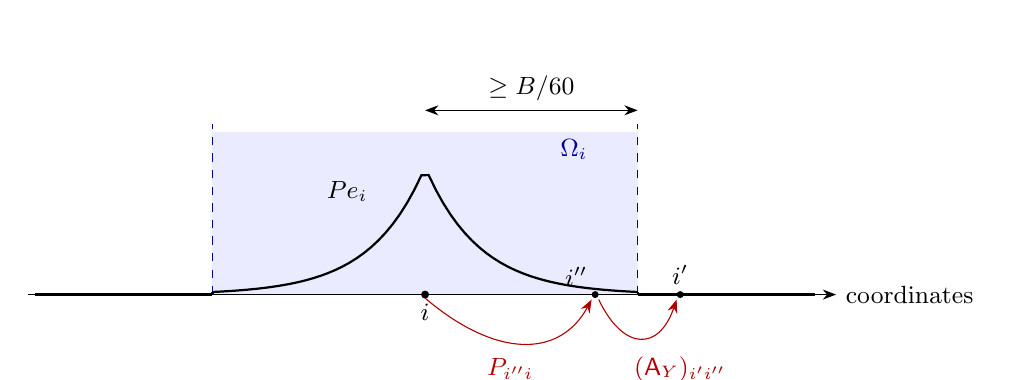
\begin{tikzpicture}[scale=0.9,>=Stealth,font=\small]
 \fill[blue!8] (-3,0) rectangle (3,2.3);
 \draw[blue!60!black,dashed] (-3,0) -- (-3,2.4) (3,0) -- (3,2.4);
 \node[blue!60!black] at (2.1,2.05) {$\Omega_i$};
 \draw[->] (-5.6,0) -- (5.8,0) node[right] {coordinates};
 \draw[thick,domain=-3:3,samples=60] plot (\x,{1.8*exp(-1.3*abs(\x))});
 \draw[thick] (-3,{1.8*exp(-3.9)}) -- (-3,0) (3,{1.8*exp(-3.9)}) -- (3,0);
 \draw[thick] (-5.5,0) -- (-3,0) (3,0) -- (5.5,0);
 \fill (0,0) circle (1.6pt) node[below] {$i$};
 \node at (-1.1,1.45) {$Pe_i$};
 \fill (2.4,0) circle (1.4pt) node[above left=-1pt] {$i''$};
 \fill (3.6,0) circle (1.4pt) node[above] {$i'$};
 \draw[->,red!70!black] (0,-0.05) .. controls (1.0,-0.9) and (1.9,-0.9) .. (2.35,-0.07);
 \draw[->,red!70!black] (2.45,-0.07) .. controls (2.8,-0.8) and (3.3,-0.8) .. (3.55,-0.07);
 \node[red!70!black] at (3.6,-1.05) {$(\mathsf A_Y)_{i'i''}$};
 \node[red!70!black] at (1.2,-1.05) {$P_{i''i}$};
 \draw[<->] (0,2.6) -- (3,2.6) node[midway,above] {$\ge B/60$};
\end{tikzpicture}
\caption{A compressed column. Inside the window $\Omega_i$, $\mathsf A_YPe_i=e_i$ exactly. At $i'\notin\Omega_i$ the residual is a sum of products $(\mathsf A_Y)_{i'i''}P_{i''i}$ with $i''\in\Omega_i$; each decays exponentially in $\operatorname{dist}(i,i'')+\operatorname{dist}(i'',i')\ge B/60$.}\label{fig:B-window}
\end{figure}

\paragraph{The differentiated local integral.}
We state the local estimate for the finite products used in the expansion. In a fixed allocation sector, join selected large-field tests when their fixed enlarged neighbourhoods intersect; the connected components $A_\eta$ are the \emph{large-field components}. Write $A(M)$ for the union of the fine-plaquette, mismatch and coarse-site selections belonging to the components chosen in a product~$M$. Fix the support enlargement $h_{\rm loc}$ once for the local factors. Compatibility means that the radius-$h_{\rm loc}B$ neighbourhoods of the distinct chosen components are disjoint.

A factor has a complete read support $S_i$ containing the projected endpoints of every link it uses, every path and relaxed threshold test in its formula, every tag and frozen link, and the entire window $\Omega_a^{\rm loc}$ for each Gaussian coordinate $a$ it reads. Thus a change outside $S_i$ leaves its formula and its Gaussian marginal unchanged. A finite product $M$ is a \emph{polymer} when the intersection graph of its supports is connected. Choose $o$ in their union. Its size $s_M$ is the sum of the numbers of radius-$B$ blocks covering these supports, including retained path lengths in the same units.

For an incoming forced activity retain its support $Y_i$ and inventory $I_i$ from Section~\ref{sec:renormalization}. The admitted products satisfy
\begin{gather*}
Y_i\cap Y_{i'}=\varnothing\quad(i\ne i'),\qquad
I_i\subset\bigcup_{p\in A_f(M)}\operatorname{corners}(p),\\
\flags_m(V)\cap\bigcup_{i\in M}S_i=\varnothing.
\end{gather*}
They also satisfy the component compatibility just specified. These conditions retain exactly the incidence and separation used in local integration.

Some incoming forced activities are only measurable, so the differentiated integral cannot be estimated by differentiating every factor in its link arguments. We instead change Gaussian coordinates as the coarse field varies, so that each physical fine link read by such an activity stays fixed. Derivatives then act on the smooth factors, the Jacobian and the Gaussian density. The nested chart cutoffs below ensure that this change is valid wherever a differentiated factor is nonzero.

\paragraph{Factors and their bounds.} The retained square corrections are the exponential differences between the exact fine or mismatch terms and their affine squares $|\mathsf Da+b_Y|^2/2$. The other smooth factors are incoming regular activities, chart densities, and determinant and Gaussian-density corrections. Incoming forced activities are bounded by their measurable supremum envelopes.

For the chart cutoffs choose a smooth $\chi:[0,\infty)\to[0,1]$ equal to one on $[0,1]$ and zero on $[2,\infty)$. On an active logarithmic coordinate put $\chi_{a_*}(u_e)=\chi(|u_e|/(a_*t_{\rm f}))$. The fixed mean bound is $|m_Y(e)|\le c_*t_{\rm f}$, and choose $a_*>c_*+1$. Fix a logarithm radius $r_{\log}>0$ and take $\refbeta_m$ large enough that $4a_*t_{\rm f}<r_{\log}/2$. The smaller chart is $|u_e|<a_*t_{\rm f}$; the broader cutoff equals one for $|u_e|\le2a_*t_{\rm f}$. A protected link is an active link accompanied by the broader cutoff $\chi_{2a_*}$ whenever an incoming measurable factor reads it. Nonactive free links are the frozen links $Y$; their physical values are held fixed. The nesting $\chi_{a_*}\ne0\Rightarrow\chi_{2a_*}=1$ is what allows the physical-link change below on all derivative supports.

Cutoff remainders are the departures from one of the fine-plaquette and mismatch cutoffs, the frame and predictor tag likelihoods, the inventory tests, or the active chart cutoffs. The addresses are fine plaquettes for fine cutoffs, coarse edges for mismatches and predictor tags, coarse sites for frame tags, fine sites for inventory tests, and fine edges for chart cutoffs. A site's location is its coarse projection; an edge or plaquette is located at its projected initial vertex. Near a large-field component the corresponding departure is included in its component factor. For each remaining cutoff remainder~$w$, the estimate below requires the remainder and all its derivatives to be supported on
\begin{equation*}
E_w=\{z:\exists i,\ \operatorname{dist}(i,\operatorname{loc}(w))\le2B,
\quad |z_i|\ge\xi t_{\rm f}/(2g)\}.
\end{equation*}
If all these coordinates are below that threshold, then $|m_Y(e)+gz_e|\le(c_*+\xi/2)t_{\rm f}<a_*t_{\rm f}$ after reducing $\xi$, so both active chart cutoffs equal one. To infer the corresponding fine-chord, mismatch, tag and inventory conclusions on every read, one also needs a retained-mask or active-domain condition that controls frozen links. The section does not yet establish that condition for all the remaining addresses; the required separation of those addresses from the selected tests is distinct from the witness radius $2B$. When these implications hold with a strict margin, the margin persists on derivative supports. Let $\mathcal J(M)$ be the set of distinct selected cutoff-remainder addresses and $E_{\mathcal J(M)}=\bigcap_{w\in\mathcal J(M)}E_w$ their simultaneous event. Their amplitudes are bounded by the fixed stage-and-ratio constant
\begin{equation*}
M_w=2+|\mathbb B_R\times S_4|+|\mathbb B_R|.
\end{equation*}
This includes the likelihood relative to uniform tags. Fix any $\tau_w>0$ before the coupling threshold, and put $\varepsilon_w=\refbeta_{m+1}^{-\tau_w}$. For a factor~$i$ that is not a cutoff remainder, $a_i$ is the product of its absolute coefficient bound (for a square correction, its deterministic envelope), its selected-test or path suppression, and the Gaussian exponential factor $\exp(C\Lambda_i)$ of Step~4 of the proof below. The weights are
\begin{equation*}
f_i=a_i\quad(i\notin\mathcal J(M)),\qquad
f_w=M_w\varepsilon_w\quad(w\in\mathcal J(M)).
\end{equation*}
Each distinct address contributes once.

\paragraph{The reference law and the transported integrand.} Assume $\beta\in\mathfrak B_{m+1}$. Use the local prescription $\Omega^{\rm loc}$ in~\eqref{eq:B-window} throughout this local integral. Conditional on the fixed sector and tags the reference law is
\begin{equation*}
d\nu=dH_F(Y)\,d\gamma_\Gamma(z).
\end{equation*}
Here $H_F$ is product Haar measure on the frozen tree-slice links and $\gamma_\Gamma$ is the centred Gaussian. Reference tags are independent uniform tags; their actual likelihoods are included among the factors. All estimates below are uniform in those tags. Table~\ref{tab:B-variables} records which variables are fixed, integrated or changed.

\begin{table}[ht]
\centering\small
\begin{tabular}{@{}p{0.2\textwidth}p{0.34\textwidth}p{0.38\textwidth}@{}}
\toprule
\raggedright Variable & \raggedright In the Gaussian calculation & \raggedright Afterwards, or as $V$ varies\tabularnewline
\midrule
\raggedright tree links & \raggedright equal to $1$ by the gauge choice & \raggedright not variables\tabularnewline
\raggedright sector data & \raggedright selected tests and block trees fixed & \raggedright fixed; derivatives keep the selected index sets\tabularnewline
\raggedright tags & \raggedright fixed; reference law uniform & \raggedright summed; actual likelihoods are factors\tabularnewline
\raggedright frozen links $Y$ & \raggedright fixed & \raggedright integrated under product Haar measure $H_F$\tabularnewline
\raggedright active coordinates & \raggedright $u=m_Y+gz$, $z\sim\gamma_\Gamma$ & \raggedright replaced by $z_V$; protected physical links stay fixed\tabularnewline
\raggedright coarse field & \raggedright base field $V_0$ & \raggedright differentiated at $V_0$\tabularnewline
\bottomrule
\end{tabular}
\caption{Variables of the differentiated local integral.}\label{tab:B-variables}
\end{table} A finite set of Gaussian reads $I$ has marginal covariance $\Gamma_I=\Gamma[I,I]$. For a finite selection write its product as
\begin{equation*}
F_M(V,Y,z)=\prod_{i\in M\setminus\mathcal J(M)}F_i(V,Y,z)
             \prod_{w\in\mathcal J(M)}W_w(V,Y,z),
\end{equation*}
where $F_i$ are the factors other than cutoff remainders and $W_w$ the cutoff remainders. The transported product uses one change of Gaussian coordinates on their common set of reads.

To differentiate while holding physical fine links fixed, fix a base coarse field $V_0$ and write $u=m_Y(V_0)+gz$. For a nearby $V$, set
\begin{equation*}
u_V(e)=\log\left(\exp(u(e))(\operatorname{rep}V_0)_e(\operatorname{rep}V)_e^{-1}\right),\qquad
z_V=g^{-1}(u_V-m_Y(V)).
\end{equation*}
Extend this formula bondwise by multiplying its displacement from $u(e)$ by a fixed smooth cutoff that is one on $|u(e)|\le r_{\log}/2$ and is supported inside the logarithm chart. For $V$ sufficiently near $V_0$, the extension is the identity plus a bounded perturbation with derivative norm strictly below one, uniformly in $u$. The contraction theorem gives a unique preimage of every point, so this is a global diffeomorphism; its Jacobian determinant remains positive. On active protected links,
\begin{equation*}
\exp(u_V(e))(\operatorname{rep}V)_e=\exp(u(e))(\operatorname{rep}V_0)_e.
\end{equation*}
Every incoming measurable activity evaluated on those links is therefore constant under this differentiation. It is bounded by its supremum majorant and no field derivative is applied to it. For example, if $V$ differs from $V_0$ only on the coarse link $(y,a)$, then $\operatorname{rep}V$ differs from $\operatorname{rep}V_0$ only on the fine edges from block~$y$ to block~$y+e_a$; on all other edges $u_V(e)=u(e)$ (inside the logarithm chart), while $z_V$ may also change on other coordinates through the mean~$m_Y(V)$; on those edges, $z_V(e)-z(e)=g^{-1}(m_Y(V_0)_e-m_Y(V)_e)$.

The density of the changed marginal, relative to the base one on the union $I$ of all reads, is
\begin{equation*}
\mathcal R_I(V,z)=|\det D_z z_{V,I}|\,
\frac{(\det\Gamma_I(V))^{-1/2}\exp[-\tfrac12z_{V,I}^T\Gamma_I(V)^{-1}z_{V,I}]}
{(\det\Gamma_I(V_0))^{-1/2}\exp[-\tfrac12z_I^T\Gamma_I(V_0)^{-1}z_I]}.
\end{equation*}
Define the transported integrand by
\begin{equation*}
\widetilde F_M(V,Y,z)=\mathcal R_I(V,z)F_M(V,Y,z_V).
\end{equation*}
The bondwise change restricts to $I$ when $I$ contains every colour coordinate of each bond it reads. The matrix in this density is the inverse of the marginal covariance $\Gamma_I$, not the compression of $\Gamma^{-1}$. The Jacobian and the Gaussian density in~$\mathcal R_I$ depend on all the reads of the product together, not factor by factor; this is why the whole product is estimated in one integral under the common law. For a fixed finite product and a sufficiently small neighbourhood of $V_0$, the displacement is bounded and the covariance has uniform positive lower and finite upper bounds. The transported density and its fixed-order derivatives are then dominated, in Lebesgue coordinates, by a polynomial times a decaying Gaussian. Together with the held-link supremum envelopes and protected cutoffs, this justifies differentiation under this finite integral. The uniform read-count and simultaneous-warning estimates needed for the expansion are proved separately in the lemma.
The next lemma bounds its ordered derivatives at $V_0$ under the same base law, including products containing incoming measurable forced activities. It is the second local input to Section~\ref{sec:partII-D}. Its bounds may depend on the fixed mismatch multiplier~$W$ and energy constant~$\kappa$ of Lemma~\ref{lem:B-D1}. Clauses (i)--(iv) are conditional on the frozen-source, retained-plateau, warning-support and localized determinant inputs identified in the proof; the present section does not yet establish those inputs for the actual expansion.

For an admitted polymer put $A=A(M)$. For a large-field component with selection $A=(A_f,A_n,A_c)$ and $A_c\ne\varnothing$, let $F_A$ contain its full local sector factor and every read meeting it. Adjoin every large-field component met by those reads. In this value estimate only, replace the healthy-support condition within this component by the consistency condition of Definition~\ref{def:B-selection}. Retain the incoming-support disjointness and inventory incidence. The other factors attached to $F_A$ have the bounds $f_i$ above; their product excludes the component's selected-test suppression and cutoff remainders already included in that component. Fix $0<\kappa'_B<\kappa$ before the coupling threshold. Let $s_A$ count the radius-$B$ blocks of its complete read support, including retained path lengths in those units. The component itself is estimated in value; derivatives fall only on attached smooth factors and the common Gaussian density. Fix the orders $k,q$ and take odd $\ell$ above the stage-data threshold. A function has \emph{upper rate}~$r$ if it is at most $C_\epsilon\refbeta_{m+1}^{r+\epsilon}$ for every $\epsilon>0$ once $\refbeta_m$ is large. Write $P=P_{j,\ell,k,q}$, of upper rate zero, and $d=d_{j,\ell,k,q}$; the large-field component bound may also depend on $\kappa'_B$. Directions and sector parameters have the restrictions of Lemma~\ref{lem:B-windows}.
\begin{lemma}[Simultaneous local integration]\phantomsection\label{lem:B-D2}
Assume $\beta\in\mathfrak B_{m+1}$, as in the reference law above.
\begin{enumerate}[label=(\roman*)]
\item Admitted polymers $M$ have integrable majorants $G_M$ for their ordered derivatives through order $k$, with
\begin{equation*}
\int G_M\,d\nu\le P(\refbeta_m)(1+s_M)^d\prod_{i\in M}f_i.
\end{equation*}
\item If $A_c=\varnothing$, the selected-test envelopes satisfy, through order $k$,
\begin{equation*}
\prod_{i\ {\rm selected\ test}}a_i\le e^{-\kappa'_B\beta t_{\rm f}^2|A|}.
\end{equation*}
\item A large-field component with $A_c\ne\varnothing$ has a value majorant $G_A$ with
\begin{equation*}
\int G_A\,d\nu\le P(\refbeta_m)(1+s_A)^d e^{-\kappa'_B\beta t_{\rm f}^2|A|}\prod_{i\ {\rm attached}}f_i.
\end{equation*}
\item Simultaneous cutoff remainders at $r$ distinct addresses have probability at most $\varepsilon_w^{2r}$.
\item Disjoint complete read supports factorize, including Haar and tag coordinates.
\end{enumerate}
\end{lemma}
The window bounds of Lemma~\ref{lem:B-windows} control the Gaussian scores and exponentials, the energy of Lemma~\ref{lem:B-D1} supplies the suppression, and finite range gives the factorization.
\begin{proof}
\emph{Step 1: the affine Gaussian substitution.} For any chart-supported $F_Y$,
\begin{align*}
\int \mathrm e^{-\beta Q_Y(a)}F_Y(a)\,da
={}&(2\pi g^2)^{n/2}(\det\Gamma)^{1/2}\mathrm e^{-\beta Q_Y(m_Y)}\\
&\times\int F_Y(m_Y+gz)
 \exp\left\{\langle\eta_Y,z\rangle+\tfrac12\langle z,(\Gamma^{-1}-\mathsf A_Y)z\rangle\right\}\,d\gamma_\Gamma(z),\\
\eta_Y={}&-g^{-1}(\mathsf A_Ym_Y+f_Y).
\end{align*}
Here $n$ counts active real coordinates; the Haar density and chart cutoffs are included in $F_Y$. Indeed, $da=g^n\,dz$ and
\begin{equation*}
\beta Q_Y(m_Y+gz)=\beta Q_Y(m_Y)
 +g^{-1}\langle\mathsf A_Ym_Y+f_Y,z\rangle
 +\tfrac12\langle z,\mathsf A_Yz\rangle.
\end{equation*}
Dividing the resulting density by the normalized $\gamma_\Gamma$ density gives both the linear residual and the quadratic correction in the displayed identity, as well as its determinant. The identity holds for every vector~$m_Y$ and every positive~$\Gamma$, in particular for either window prescription. The choices~\eqref{eq:B-window} only make the reference law finite range; the exponents of the retained factor vanish exactly when $m_Y=-\mathsf A_Y^{-1}f_Y$ and $\Gamma=\mathsf A_Y^{-1}$, and Step~4 estimates that factor. The local expansion in Section~\ref{sec:partII-D} uses $\Omega^{\rm loc}$.

For the window part of the correction, put $\mathsf E_\Gamma=\mathsf A_Y\Gamma-I$. When $B$ is sufficiently large, Lemma~\ref{lem:B-windows} gives $\|\mathsf E_\Gamma\|_{\rm Schur}<1$, and therefore
\begin{align*}
\Gamma^{-1}-\mathsf A_Y
 &=\sum_{h\ge1}(-\mathsf E_\Gamma)^h\mathsf A_Y,\\
\log\det\Gamma+\log\det\mathsf A_Y
 &=\sum_{h\ge1}\frac{(-1)^{h+1}}{h}\operatorname{tr}(\mathsf E_\Gamma^h).
\end{align*}
The order in the first series follows from $\mathsf A_Y\Gamma=I+\mathsf E_\Gamma$; the second uses positivity of $\mathsf A_Y$ and~$\Gamma$. The same estimates give convergence after any fixed number of derivatives, with the selected windows held fixed. Expanding the matrix products gives ordered chains of coordinate indices; their complete reads include the windows and the row stencils at every link of the chain. In an exponentially weighted Schur norm, the absolute sum over either endpoint of a length-$h$ quadratic chain, at fixed other endpoint, is bounded by $\||\mathsf E_\Gamma|\|_{\rm Schur}^h\||\mathsf A_Y|\|_{\rm Schur}$. Fixed-order derivatives add at most a fixed polynomial in~$h$, and a smaller exponential weight absorbs the spatial direction weights. For a selected collection of quadratic chain terms, $|z_i z_{i'}|\le(z_i^2+z_{i'}^2)/2$ assigns each absolute term to its endpoints; summing the two endpoint marginals before Gaussian integration controls the whole collection without a bound on the number of chains at one anchor. These identities isolate the window correction relative to $\mathsf A_Y^{-1}$; they do not identify $\det\mathsf A_Y$ with the stationary determinant of Lemma~\ref{lem:B4}.

\emph{Unresolved localization.} The endpoint estimate alone does not prove the support-weighted summability of the resulting ordered chains with their complete window and field reads. The proof also needs a separate comparison of $\det\mathsf A_Y$ and the stationary determinant, including the selected allocation and its scalar factors. Until those two inputs are established for the same sector, the determinant and covariance factor bounds used in Step~4 and in Lemma~\ref{lem:D-connected} are conditional.

\emph{Step 2: scores.} For the common change of coordinates defined above, the first logarithmic derivative of the Gaussian density is
\begin{equation*}
-\tfrac12\tr(\Gamma_I^{-1}\dot \Gamma_I)
+\tfrac12z_V^T\Gamma_I^{-1}\dot \Gamma_I\Gamma_I^{-1}z_V
-z_V^T\Gamma_I^{-1}\dot z_V.
\end{equation*}
Add the logarithmic Jacobian derivative. Repeated differentiation bounds every score through order $k$ by a polynomial in the absolute values of the marginal Gaussian coordinates, with coefficients controlled by Lemma~\ref{lem:B-windows} and the fixed smooth chart extension. The number of placements is a fixed polynomial in $1+s_M$, since $k$ is fixed and $|I|\le C_{j,\ell}B^4s_M$. Connectivity and the chosen root bound all distances from $o$ by $C_{j,\ell}B(1+s_M)$, so the spatial direction weights give another fixed polynomial.

The normalized coarse directions have size $O(t_{\rm c})$ with their stated spatial weights. On a fixed chart, derivatives of its multiplication, logarithm and bounded extension are bounded. The mean derivatives are $O(t_{\rm f})$, while $t_{\rm c}/t_{\rm f}$ stays bounded. In $z_V$ the additional normalization is $g^{-1}$. Thus the score coefficients are bounded by a fixed power of $g^{-1}t_{\rm c}$, $B$ and $1+s_M$. Since
\begin{equation*}
g^{-1}t_{\rm c}\le C\exp\{(\log\log\refbeta_{m+1})^2\},
\end{equation*}
all fixed powers have upper rate zero. The small inverse and stationarity residuals in Lemma~\ref{lem:B-windows} have the same property after this normalization.

\emph{Step 3: square corrections.} The chart-supported square corrections have deterministic envelopes: on their support all logarithms are $O(t_{\rm f})$, the affine remainder is $O(t_{\rm f}^2)$, and $|\tfrac12|r+e|^2-\tfrac12|r|^2|\le |r||e|+|e|^2/2$ gives an energy correction $O(\beta t_{\rm f}^3)$. The exponentially summable path coefficients bound the same quantities with fixed path-length powers after differentiation. These bounds enter $a_i$.

This use of the small logarithms also requires a same-field plateau for every frozen link read by a retained row, or a separately bounded factor for a failed plateau. The stated consistency of Definition~\ref{def:B-selection} reaches $5B$, whereas the active/frozen boundary is at $10B$; the proof here does not yet show that the necessary physical cutoff and tag factors remain on that boundary after the expansion. Thus the claimed square-correction and annular bounds in this step and in Steps~7--8 are conditional on that missing support argument. Exact compensation of the surrogate in the density does not by itself make the remainder small.

\emph{Step 4: unbounded exponentials.} The unbounded exponentials come from the residual Gaussian density and its local covariance comparisons. Write their upper exponents as $\eta_i\cdot z+z^TK_i z/2$, with $K_i\ge0$. At the base field the Gaussian likelihood is one; its derivatives are the polynomial scores already estimated. Its exponent tends to zero with $V-V_0$, so on a sufficiently small neighbourhood its weighted row sums are at most $\delta_B=C_{j,k}B^d \mathrm e^{-cB}$. The residual Gaussian density has this bound by Lemma~\ref{lem:B-windows}. The resolvent identity for each compressed inverse gives $C\delta_B$ for its local quadratic corrections. For the finitely many types of test and covariance-ratio addresses, bounded multiplicity and decay from the address bound their sum at coordinate~$a$ by $C\delta_B\sum_y\mathrm e^{-c\operatorname{dist}(y,a)}\le C'\delta_B$. For the arbitrarily many ordered defect chains use instead the two endpoint Schur sums of Step~1. The support-weighted factorization of these chains remains conditional on the localization input stated there. In the linear terms, weighted Cauchy--Schwarz at each coordinate gives
\begin{equation*}
\left|\Gamma^{1/2}\sum_i\eta_i\right|^2
 \le C\sum_i\Lambda_i,\qquad
\left\|\Gamma^{1/2}\sum_iK_i\Gamma^{1/2}\right\|\le C\delta_B.
\end{equation*}
To specify the linear bound, let $w_{ia}$ be the sum of the absolute path weights contributing to coordinate $a$ of $\eta_i$; bounded endpoint multiplicity gives $\sup_a\sum_i w_{ia}\le C$. Put
\begin{equation*}
\Lambda_i=\sum_a\frac{|\eta_i(a)|^2}{w_{ia}}+\tr(\Gamma^{1/2}K_i\Gamma^{1/2}),
\end{equation*}
with zero summand if both numerator and denominator vanish. This quantity assigns the common linear exponential bound to the individual factors. To see the first bound, use $|\sum_r x_r|^2\le(\sum_r w_r)\sum_r|x_r|^2/w_r$ with the absolute path weights $w_r$; their sums are the preceding bounded row sums. The Schur bound for $\Gamma$ completes the estimate. In particular, this bounds $|\Gamma^{1/2}\eta_0|^2$ with $\eta_0=\sum_i\eta_i$, including all terms $\eta_i^T\Gamma\eta_{i'}$ with $i\ne i'$. This is the factor $\exp(C\Lambda_i)$ in $a_i$. Put $K=\sum_iK_i$. Since $0\le K_i\le K$, each $\|\Gamma^{1/2}K_i\Gamma^{1/2}\|$ is at most $\|\Gamma^{1/2}K\Gamma^{1/2}\|<1/8$ for large $B$, also after the fixed enlargement needed for two moments.
Diagonalization and square completion, with $-\log(1-u)\le2u$ for $0\le u\le1/2$, give
\begin{equation*}
\mathbb E_\Gamma \mathrm e^{2\eta_0\cdot z+z^TKz}
 \le\exp\!\left(C\sum_i\Lambda_i\right).
\end{equation*}
Under this tilt the covariance is at most $2\Gamma$ and its mean is $(I-2\Gamma K)^{-1}(2\Gamma\eta_0)$. Polynomial moments are bounded by the preceding linear estimate; increasing the fixed constant in $\exp(C\Lambda_i)$ includes their mean contributions.
Thus the differentiated factors and likelihood have, after removing the cutoff-remainder amplitudes, one $L^2$ majorant bounded by $P_{j,\ell,k,q}(\refbeta_m)(1+s_M)^d\prod a_i$.

\emph{Step 5: cutoff remainders.} We next bound the simultaneous event defined above, including all derivative supports. Let $p_0$ bound the number of Gaussian coordinates per coarse site and $m_0$ the number of distinct cutoff-remainder addresses per site. These are fixed once the stage and ratio are fixed. For $r$ distinct addresses, choose one violating coordinate, a \emph{witness}, for each. There are at most $(p_0|\mathbb B_{2B}|)^r$ choices. Distinct addresses may share a witness, but a single coordinate can serve at most $m_0|\mathbb B_{2B}|$ addresses, so the set~$J$ of distinct witnesses satisfies
\begin{equation*}
r\le m_0|\mathbb B_{2B}|\,|J|,\qquad |J|\le r.
\end{equation*}
The Schur bound gives covariance operator norm at most $M_0$. The exponential Markov inequality for each signed sum $\sum_{i\in J}\pm z_i$, and summation over the $2^{|J|}$ signs, give
\begin{equation*}
\Pr\{|z_i|\ge T\ (i\in J)\}\le2^{|J|}\exp\{(M_0/2-T)|J|\}.
\end{equation*}
Take $T=\xi t_{\rm f}/(2g)$ and choose $H>0$ with $M_0/2+Hm_0|\mathbb B_{2B}|\le T$. Then $(T-M_0/2)|J|\ge Hm_0|\mathbb B_{2B}||J|\ge Hr$: although witnesses are shared, the large deviations still gain $\mathrm e^{-H}$ per address. Summing over the witness choices gives
\begin{equation*}
\Pr(E_{\mathcal J(M)})\le(p_0|\mathbb B_{2B}|)^r\,2^r\mathrm e^{-Hr}=
\bigl(2p_0|\mathbb B_{2B}|\mathrm e^{-H}\bigr)^r.
\end{equation*}
The factor $t_{\rm f}/g$ grows faster than every fixed power of $B$ and $\log\refbeta_{m+1}$. Consequently $H$ can exceed $2\tau_w\log\refbeta_{m+1}+\log(2p_0|\mathbb B_{2B}|)$, proving~(iv). A cutoff remainder is thus rare because its violating coordinate lies $t_{\rm f}/g\gg1$ standard deviations out.

The probability calculation is conditional on the excursion implication stated before the lemma. For a cutoff that reads frozen links, the implication needs the actual retained component masks or a verified physical-link plateau; a small Gaussian vector alone does not control arbitrary frozen Haar variables. In particular, separation of a warning address from selected tests is a separate condition from the radius $2B$ of its Gaussian witness. This missing implication also leaves the application of~(iv) conditional.

\emph{Step 6: the common majorant.} Take the finite sum of the absolute differentiated smooth expressions and scores, multiplied by the fixed incoming measurable envelopes, the cutoff-remainder amplitudes $\prod_wM_w$, and the simultaneous indicator. The product rule bounds every derivative through order $k$ by this same nonnegative function~$G_M=G_M^0\mathbf 1_{E_{\mathcal J(M)}}$. By the Cauchy--Schwarz inequality, Step~4 and~(iv),
\begin{equation*}
\int G_M\,d\nu\le\|G_M^0\|_{L^2(\nu)}\Pr(E_{\mathcal J(M)})^{1/2}
\le P(\refbeta_m)(1+s_M)^d\prod_{i\notin\mathcal J(M)}a_i\prod_{w\in\mathcal J(M)}M_w\,\varepsilon_w,
\end{equation*}
so the square root of the simultaneous bound leaves exactly one factor~$\varepsilon_w$ per address. Since $f_w=M_w\varepsilon_w$, this proves~(i).

\emph{Step 7: selected-test suppression.} Distribute the local energy of Lemma~\ref{lem:B-D1} among the selected-test factors before differentiating. When $A_c=\varnothing$ the admitted support is healthy. The physical-link change holds the fine links and selected test indices fixed; differentiated test cutoffs retain the selected-test inequalities on their supports. The exponential energy is retained in each differentiated envelope. Annular affine errors have size $E(\refbeta_m)|A|$ with $E$ of upper rate $-3/2$, and the remaining per-test logarithmic corrections have a fixed-power bound $C_{j,\ell,k,q}(1+\log\refbeta_{m+1})^{d_0}|A|$. Derivatives of the smooth factors through order $k$ multiply this bound by fixed powers of $B$, $g^{-1}t_{\rm c}$ and the number of selected tests. Their logarithms per test are $o(\beta t_{\rm f}^2)$, since $\beta t_{\rm f}^2$ is comparable to $(\cutoffsize_{m+1})^2$, which exceeds every fixed power of $\log\refbeta_{m+1}$. Also $E(\refbeta_m)/t_{\rm f}^2\to0$. Increase the coupling threshold after fixing $\kappa'_B<\kappa$; absorption into $(\kappa-\kappa'_B)\beta t_{\rm f}^2|A|$ gives~(ii) through order $k$. The support factor $(1+s_M)^d$ remains outside this per-test estimate. The determinant and covariance corrections use the exponential bounds above. Integrating the independent frozen Haar variables and summing the finite tag probabilities preserve the bound.

\emph{Step 8: large-field components.} Retain the full sector masks of the component and all frozen links read by it. The lower bound in Lemma~\ref{lem:B-D1} gives $\kappa t_{\rm f}^2|A|$ in its local energy. The enlarged neighbourhood used by the component adds annular affine remainders bounded by $E(\refbeta_m)|A|$, where $E$ has upper rate $-3/2$: the term error is $O(t_{\rm f}^3)$, and the number of positions per test is a fixed power of $B$. The chart-density, tag, local determinant and normalized frozen-coordinate factors contribute at most $C_{j,\ell}(1+\log\refbeta_{m+1})^{d_0}|A|$ to the upper exponent, for a fixed $d_0$. Indeed, their read counts are at most $C_{j,\ell}B^4|A|$; the logarithm of each inverse Gaussian normalization is $O(1+\log\refbeta_{m+1})$, the chart logarithms are bounded on the protected chart, and the local determinant terms have the bounds of Lemma~\ref{lem:B-windows}. The retained value envelope is thus at most
\begin{equation*}
\exp\!\left[-\kappa\beta t_{\rm f}^2|A|+
 \{\beta E(\refbeta_m)+C_{j,\ell}(1+\log\refbeta_{m+1})^{d_0}\}|A|\right].
\end{equation*}
As in Step~7, both corrections are $o(\beta t_{\rm f}^2)$ per test. Choose $\kappa''_B$ strictly between $\kappa'_B$ and $\kappa$ and increase the coupling threshold. This bounds the component envelope by $e^{-\kappa''_B\beta t_{\rm f}^2|A|}$. Use this component envelope and the incoming measurable supremum envelopes. The attached factors and Gaussian scores have exactly the $L^2$ bound proved above. Cauchy--Schwarz with their simultaneous event retains every attached $f_i$. Polynomial factors in the number of component reads are bounded by a fixed polynomial in $1+s_A$ times a fixed power of $B$, the latter entering $P$. Any remaining fixed per-test logarithmic loss is absorbed by $\kappa''_B-\kappa'_B$. Frozen Haar integration has mass one. This proves~(iii), without differentiating its flag masks or taking a supremum of a Gaussian coordinate.

\emph{Step 9: factorization.} The Gaussian marginal on $I$ has covariance $\Gamma_I$. Every complete read support contains $\Omega_i^{\rm loc}$ for each coordinate $i$ it reads. The windows are symmetric. Hence if $i,i'$ belong to disjoint complete read supports, $i'\notin\Omega_i^{\rm loc}$ and $i\notin\Omega_{i'}^{\rm loc}$, so $\Gamma_{ii'}=0$ by~\eqref{eq:B-window}. The Gaussian characteristic function therefore factorizes over these supports. The frozen Haar and reference tag coordinates are disjoint as well, proving~(v).
\end{proof}

\section{Path actions and the one-loop coupling}\label{sec:partII-C}

After each integration the effective action keeps its curvature terms through fourth order in a path action. Its quadratic part is normalized so that $\beta$ is the coefficient of the squared Wilson curvature at zero momentum at every level. The quadratic terms independent of $\beta$, the loop atoms, have vanishing zeroth and first displacement moments, so they carry no curvature-square term. This section constructs these arrays and computes the one-loop coefficient of an auxiliary fine determinant. Subject to the inserted-strip bounds identified in Lemma~\ref{lem:C6}, the comparison transfers that coefficient to the blocked determinant, lowering its curvature-square coefficient by $\slope\log\ell_m$ up to an error bounded independently of the block ratio (Lemma~\ref{lem:C7}).

The path bounds enter Theorem~\ref{prop:MT}, and the coefficient $\alpha_{N,m}$ enters Theorem~\ref{prop:RG}. Section~\ref{sec:partII-B} supplies the inputs. The free forms and their row factor (Lemma~\ref{lem:B2}) fix the quadratic part; the stationary interpolation and the vertex bounds (Lemmas~\ref{lem:B3} and~\ref{lem:B5}) give the classical cubic and quartic terms; the Gaussian coordinates, the inverse insertions and the Ward estimates (Lemmas~\ref{lem:B4}, \ref{lem:B7} and~\ref{lem:B6}) control the determinant. The scalar reset of the coupling uses the activities of Section~\ref{sec:partII-D} and is proved there, in Section~\ref{subsec:C-reset}.

Throughout, the group and metric are those of Definition~\ref{def:D01}, and the scales are those of Section~\ref{sec:renormalization}. At a step $m+1\to m$ put $\ell=\ell_m$ and $j=J_{m+1}$. The path arrays (row coefficients and atoms of Definition~\ref{def:D22}) depend on $N,m$ and the intervening block ratios, and are chosen on $\Z^4$ before periodic evaluation. They are independent of the volume index~$p$ and of the running coupling. Constants declared uniform in~$\ell$ are chosen before~$\ell$.

The arrays are constructed by descending induction on~$m$. Write $(I_m)$ for the path bounds and cancellations of Lemmas~\ref{lem:C1}--\ref{lem:C2} at level~$m$, the path part of the induction scheme of Section~\ref{sec:partII-B}. The top-level Wilson matching in the proof of Lemma~\ref{lem:C4} starts the induction. Under $(I_{m+1})$, Lemmas~\ref{lem:C4}, \ref{lem:C6} and~\ref{lem:C7} treat the step $m+1\to m$; the joint proof after Lemma~\ref{lem:C7} constructs the output arrays and proves~$(I_m)$. Curl division and the gauge determinant identity are independent of this induction.

\subsection{Curvature coordinates and the path action}\label{subsec:C-coordinates}

A path transports curvature to an anchor, where invariant colour contractions can be taken. Write $U_\gamma$ for the ordered link product along~$\gamma$, $\mathfrak p=(a,b)$, $a<b$, for an orientation, and $U_{x;\mathfrak p}$ for a plaquette holonomy. The footprint of a slot is the set of vertices visited by its path and plaquette boundary. The footprint of an atom is the union of its slot footprints and the origin, translated to its anchor. Recall that a set is healthy if it avoids $\flags_m(U)$ (Section~\ref{sec:renormalization}); an atom is masked by the health of its footprint.

\begin{definition}[Curvature slots]\label{def:D22}
A slot $s=(\gamma,\mathfrak p)$, with $\gamma:0\to z_s$, has length $|\gamma|+4$ and value
\begin{equation*}
\mathcal F_s(U,x)=\operatorname{Ad}(U_{x+\gamma})\operatorname{proj}_{\g}
\frac{U_{x+z_s;\mathfrak p}-U_{x+z_s;\mathfrak p}^{-1}}2\,.
\end{equation*}
Transport is from $x+z_s$ to~$x$. Set $\mathcal L_{\mathfrak p}^{\rm path}=\sum_i r_{\mathfrak p i}\mathcal F_{\mathfrak p i}$. For $k=2,3,4$, the atoms $\mathfrak a_i^{(k)}$ are real invariant $k$-linear expressions in slots, masked by health on their footprints. Atom length sums slot lengths; $|\mathfrak a_i^{(k)}|$ sums absolute colour coefficients. These arrays retain local terms through fourth order.
\end{definition}

Here $r_{\mathfrak p i}\in\R$ and $\mathcal F_{\mathfrak p i}$ denotes the slot assigned to row~$\mathfrak p$ and index~$i\in\N$. In the orthonormal colour basis $(e_b^{\g})_b$ of Definition~\ref{def:D01}, an atom has the form
\begin{equation*}
\mathfrak a_i^{(k)}(U,x)=\mathbf1_{X_i+x\,\mathrm{healthy}}
\sum_{b_1,\ldots,b_k} c_i(b_1,\ldots,b_k)
\prod_{\nu=1}^k\langle e_{b_\nu}^{\g},\mathcal F_{s_{i,\nu}}(U,x)\rangle_{\g}\,.
\end{equation*}
The coefficients are invariant under the simultaneous adjoint action on all slots, and $X_i$ is the footprint just defined.

For each stage~$k$, take $\gamma_k>0$ from Lemma~\ref{lem:B2}, so the free plaquette forms for the top and both incoming stages are at least $2\gamma_k I$. Write $c_{\rm dir}=c_{{\rm dir},J_m}$ and $c_{\rm lin}=c_{{\rm lin},J_m}$. Whenever $c_{\rm dir}\le\gamma_{J_m}$, the form $\mathsf H_{N,m}-c_{\rm dir}I$ below is at least $\gamma_{J_m}I$ and has the positive row factor used below.

\begin{definition}[Path action]\label{def:D23}
At level $m$ the path action $\pathaction_{N,m}$ is~\eqref{eq:I12-path-action}, with the clip and relaxed threshold test of~\eqref{eq:I12-clipping}, the rows and atoms of Definition~\ref{def:D22}, and clipping constants $0<16c_{\rm lin}<c_{\rm dir}\le\min(\gamma_{J_m},1)$. Write
\begin{equation*}
\pathaction_{N,m}(\beta,U)=\beta\mathsf K^{\rm kin}_m(U)+\mathcal L_m(U),
\end{equation*}
where $\mathsf K^{\rm kin}_m$ is the hypercubic average of the clipped plaquette terms, the row squares and the cubic and quartic atoms, and $\mathcal L_m$ that of the quadratic atoms.
\end{definition}

The kinetic part carries the coupling; the loop part collects the quadratic corrections that do not scale with~$\beta$. The clip drops at $u=t$ from $c_{\rm dir}t^2/2$ to $c_{\rm lin}t^2$, and its linear branch gives $\operatorname{clip}_t(u)=c_{\rm lin}tu\ge c_{\rm lin}t^2$ for $u>t$. This positive linear large-field branch is the lower bound used in the local large-field energy estimate, Lemma~\ref{lem:B-D1}, and through it in the forced bounds of Lemma~\ref{lem:D-connected}. Because of the jump the path action is only Borel in the links. The derivatives used later are taken on healthy configurations, where every clip of the support is on its quadratic branch and every mask is fixed, and coupling derivatives hold the physical links and the masks fixed (Section~\ref{subsec:D-analytic}). No derivative of a flag boundary or of the clip is ever taken.

\begin{lemma}[Path bounds]\label{lem:C1}
For every $N$ and $m\le N$ the chosen arrays are independent of $p$ and~$\beta$. There are widths $0<w^{\rm path}_k<w'_k$ and amplitudes $A^{\rm path}_k>0$, depending only on the stage~$k$, such that, uniformly in~$N$, with $w=w'_{J_m}$,
\begin{align*}
\sum_i|r_{\mathfrak p i}|e^{w\operatorname{length}(\mathcal F_{\mathfrak p i})}&\le A_{J_m}^{\rm path},\\
\sum_i|\mathfrak a_i^{(k)}|e^{w\operatorname{length}(\mathfrak a_i^{(k)})}
&\le\begin{cases}\Lambda_m^{\rm loop},&k=2,\\A_{J_m}^{\rm path},&k=3,4,\end{cases}
\end{align*}
where $\Lambda_m^{\rm loop}=2(\cutoffsize_m)^{\theta_{J_m}}$ depends on the level. A fortiori these bounds hold at width $w^{\rm path}_{J_m}$.
\end{lemma}

The joint proof of Lemmas~\ref{lem:C1} and~\ref{lem:C2} follows Lemma~\ref{lem:C7}. To state the cancellations, put
\begin{equation*}
s_{\mathfrak p\mathfrak q}=\sum_{i:\,\operatorname{orientation}(\mathcal F_{\mathfrak p i})=\mathfrak q}r_{\mathfrak p i}\,.
\end{equation*}
For ordered orientations $\mathfrak q,\mathfrak r$ let $I_{\mathfrak q\mathfrak r}$ be the set of quadratic atoms whose two slots have orientations $\mathfrak q,\mathfrak r$, with colour coefficients $c_i(b_1,b_2)$ and slot offsets $z_{i,1},z_{i,2}$.

The cancellations have a Fourier meaning. To quadratic order in the links, an atom in $I_{\mathfrak q\mathfrak r}$ pairs the curvatures at two points displaced by $z_{i,2}-z_{i,1}$, so the loop atoms contribute the plaquette-kernel symbol $\sum_{i\in I_{\mathfrak q\mathfrak r}}c_i(b_1,b_2)e^{i\xi\cdot(z_{i,2}-z_{i,1})}$ between two curvatures. A zero total coefficient removes its constant term and a zero first displacement moment removes its linear term, so the symbol is $O(|\xi|^2)$. Each curvature is a curl, of order $|\xi|$ in the link variables. Hence the loop atoms have a link kernel of order four and contain no curvature-square term: the marginal curvature square is carried by the coupling alone. Under blocking, the cell volume $\ell^4$, the two interpolated fields $\ell^{-2}$ and the rescaled momentum $\xi/\ell$ turn an order-four link kernel into $\ell^4\ell^{-2}O(|\xi/\ell|^4)=\ell^{-2}O(|\xi|^4)$, an inverse-block-square gain (proof of Lemmas~\ref{lem:C1}--\ref{lem:C2}).

\begin{lemma}[Kinetic and quadratic cancellations]\label{lem:C2}
For all orientations $\mathfrak q,\mathfrak r$ and colours $b_1,b_2$,
\begin{equation*}
c_{{\rm dir},J_m}\delta_{\mathfrak q\mathfrak r}+
\sum_{\mathfrak p}s_{\mathfrak p\mathfrak q}s_{\mathfrak p\mathfrak r}=\delta_{\mathfrak q\mathfrak r},
\qquad
\sum_{i\in I_{\mathfrak q\mathfrak r}}c_i(b_1,b_2)=0,
\qquad \sum_{i\in I_{\mathfrak q\mathfrak r}}c_i(b_1,b_2)(z_{i,2}-z_{i,1})=0\,.
\end{equation*}
All these moment series converge absolutely.
\end{lemma}
Thus the kinetic part has the Wilson normalization $\widehat{\mathsf H}_{N,m}(0)=I$ below, and the loop atoms do not change the curvature-square coefficient.

\subsection{Fourth-order matching}\label{subsec:C-matching}

Near the flat field all relaxed threshold tests equal one. By $\chord^2=2\wilsonterm$ from~\eqref{eq:I12-price-chord}, the leading analytic action is obtained from Definition~\ref{def:D23} by replacing the clipped term by $c_{\rm dir}\wilsonterm$ and omitting the indicators and loop atoms. Denote this action, without its factor~$\beta$, by $\mathsf S_{N,m}$. Its prescribed quadratic part is
\begin{equation*}
\frac12\langle d_1a,\mathsf H_{N,m}d_1a\rangle,
\qquad \mathsf H_{N,m}=c_{{\rm dir},J_m}I+\rho_{N,m}^*\rho_{N,m},
\qquad \widehat{\mathsf H}_{N,m}(0)=I\,.
\end{equation*}
Here $d_1$ is the lattice curl. Lemma~\ref{lem:B2} gives the exact adjacent free relation and the row factor $\rho_{N,m}$, with $\mathsf H_{N,m}-c_{{\rm dir},J_m}I\ge\gamma_{J_m}I$. The rows are read off from $\rho_{N,m}$. Write $(\rho_{N,m}F)_{\mathfrak p}(x)=\sum_{\mathfrak q}\sum_{z\in\Z^4}\rho_{\mathfrak p\mathfrak q}(z)F_{\mathfrak q}(x+z)$. For each $\mathfrak p,\mathfrak q,z$ with $\rho_{\mathfrak p\mathfrak q}(z)\ne0$ take one slot $(\gamma_z,\mathfrak q)$, with $\gamma_z$ a fixed coordinate path from $0$ to $z$, and row coefficient $\rho_{\mathfrak p\mathfrak q}(z)$. At the flat field $\mathcal L^{\rm path}_{\mathfrak p}(U,x)$ linearizes to $(\rho_{N,m}d_1a)_{\mathfrak p}(x)$, so the direct and row terms have quadratic part $\frac12\langle d_1a,\mathsf H_{N,m}d_1a\rangle$; also $s_{\mathfrak p\mathfrak q}=\widehat\rho_{\mathfrak p\mathfrak q}(0)$, and the exponential decay of $\rho_{N,m}$ gives the row bound of Lemma~\ref{lem:C1}. The cell volume contributes $\ell^4$ and each curvature contributes $\ell^{-2}$; hence $\ell^4(\ell^{-2})^2=1$, preserving the coefficient~$\beta$.

We need a division that expresses a gauge-invariant Taylor difference in curvatures. For a momentum~$\xi$ put $q_a(\xi)=e^{i\xi_a}-1$; its exterior action $d_1(\xi)a=q(\xi)\wedge a$ is the curl symbol. Momentum order~$s$ means vanishing of all Taylor coefficients of total momentum degree less than~$s$.

\begin{lemma}[Curl division]\label{lem:C3}
Let $k\ge2$, $s\ge0$ an integer, $\sigma>0$, $A\ge0$, and let $f$ be a periodic analytic kernel in independent momenta $\xi_1,\ldots,\xi_{k-1}$ ($\xi_0=-\sum_\nu\xi_\nu$), valued in $\bigotimes_{\nu=0}^{k-1}\Lambda^1\C^4$, bounded coordinatewise by $A$ on $|\operatorname{Im}\xi_\nu^a|<\sigma$, and transverse in every leg: $\delta_\nu f=0$, $\delta_\nu=\iota_{q(\xi_\nu)}$. If $k=2$ assume also momentum order $s+2$. Then there are $0<\eta\le\sigma$ and $K\ge0$, depending only on $k,\sigma$, and a periodic analytic $g$ valued in $\bigotimes_\nu\Lambda^2\C^4$, of order $s$ if $k=2$, with
\begin{equation*}
f=\delta_0\cdots\delta_{k-1}g,\qquad \sup_{\eta\text{-strip}}|g|\le KA\,.
\end{equation*}
The Fourier coefficients of $g$ decay exponentially.
\end{lemma}
In words: a gauge-invariant multilinear kernel factors through the curls of its legs.

\begin{proof}
Dividing one leg by its curl is straightforward when its momentum is independent of the others. The difficulty is the leg with momentum $\xi_0$: a primitive in that leg may fail to remain transverse in another leg. We first construct the one-leg homotopy, then correct this transversality defect. Each correction reduces the number of independent momenta by one and raises the exterior degree in the dependent leg by two, and the iteration terminates when that degree exceeds four. The two-leg case instead uses the extra vanishing order at zero momentum.

Scalar division requires vanishing when the divided leg has zero momentum; positive exterior degree requires only closedness. For one leg let $\delta=\iota_q$ be contraction on exterior tensors. Split a $\delta$-closed tensor as $f=e_a\wedge u+v$, with $u,v$ containing no $e_a$. Define
\begin{equation*}
D_af(\xi)=\frac{f(\xi)-f(\xi)|_{\xi_a=0}}{q_a(\xi)},
\qquad h_af=e_a\wedge D_av,
\qquad R_af=v|_{\xi_a=0}\,.
\end{equation*}
Here $D_a$ is the one-leg exterior division~\eqref{eq:B-exterior-division}. The identity $\delta f=0$ gives $\delta'v=-q_au$, where $\delta'$ contracts the other axes. Since $q_b$ is independent of $\xi_a$ for $b\ne a$, $D_a$ commutes with~$\delta'$, and $D_a(q_au)=u$. Consequently
\begin{equation*}
\delta h_af=q_aD_av-e_a\wedge D_a\delta'v
=v-v|_{\xi_a=0}+e_a\wedge u=f-R_af\,.
\end{equation*}
The remainder $R_af$ is again closed and has no component containing~$e_a$. Applying this in the four axes gives the homotopy
\begin{equation*}
f=\delta\left(\sum_{a=1}^4h_aR_{a-1}\cdots R_1f\right)+R_4R_3R_2R_1f\,.
\end{equation*}
The final remainder vanishes in positive exterior degree because it contains none of the four axes. In degree zero it is the restriction to zero momentum of this leg, which must vanish for scalar division. In that case the formula reads $f=\sum_aq_aD_a(R_{a-1}\cdots R_1f)$.

The quotients are analytic even at the zeros of~$q_a$. On a Fourier monomial the identity
\begin{equation*}
\frac{e^{in\xi_a}-1}{e^{i\xi_a}-1}=
\begin{cases}\sum_{v=0}^{n-1}e^{iv\xi_a},&n>0,\\
-\sum_{v=n}^{-1}e^{iv\xi_a},&n<0,\\0,&n=0\end{cases}
\end{equation*}
bounds the quotient on a smaller strip by a constant times $|n|$ times its original exponential weight. The strip loss absorbs $|n|$, so the Fourier series converges absolutely. Each division loses at most one momentum order.

For independent legs, their remaining transverse subspaces do not depend on the divided momentum, so each restriction and division preserves them. The dependent-leg induction has the following claim: with $r$ independent momenta and dependent exterior degree $d\ge1$, a tensor closed in the dependent leg and transverse in all independent legs has a dependent-leg primitive preserving those transverse conditions, provided $d+2r>4$. Analytic bounds hold after a strip reduction depending only on $r,d$ and the original strip. For $r=0$ the condition gives $d>4$, so the tensor is zero. The induction step below reduces $(r,d)$ to $(r-1,d+2)$, preserving the condition. Initially $r=k-1,d=1$, so it applies for $k\ge3$.

For the dependent momentum $\xi_0=-\sum_{i=1}^{k-1}\xi_i$, first shear the coordinates to replace $\xi_1$ by~$\xi_0$. The other independent contractions remain unchanged. The one-leg formula gives $\delta_0X=f$, retaining the contractions in legs $2,\ldots,k-1$. Write $c_1$ for contraction in leg~$1$. Its defect obeys $\delta_0(c_1X)=c_1f=0$. Solve $\delta_0Y=c_1X$ by the same formula. After $c_1$, leg~$1$ has exterior degree zero, so restoring that leg will require only scalar division.

On $\xi_1=0$, the restriction $Y_0$ is $\delta_0$-closed, since $c_1X$ vanishes there. The induction hypothesis with one fewer independent momentum and dependent degree two higher gives $\delta_0Z=Y_0$, preserving the other transverse conditions. Extend~$Z$ independently of~$\xi_1$. Then $Y'=Y-\delta_0Z$ vanishes on $\xi_1=0$, and scalar division gives $c_1D=Y'$. Thus
\begin{equation*}
V=X-\delta_0D,\qquad \delta_0V=f,\qquad c_1V=c_1X-\delta_0Y'=0\,.
\end{equation*}
All corrections preserve the other independent contractions. The two successive solves $f\mapsto X$ and $c_1X\mapsto Y$ each raise the dependent exterior degree by one; contraction $c_1$ changes only leg~$1$. Thus the restricted problem for $Y_0$ has one fewer independent momentum and dependent degree two higher. For three or more legs it terminates above exterior degree four, where the tensor is zero. The independent-leg divisions then finish the factorization.

For two legs, the restriction $Y_0$ is at zero external momentum. Starting from order $s+2$, the first division loses one order, contraction restores one, and the solve for~$Y$ leaves order $s+1\ge1$. Hence $Y_0=0$ directly. The correction and final division leave order~$s$. This verifies the scalar vanishing hypothesis where it is needed. For the Taylor differences of Definition~\ref{def:D23}, gauge invariance supplies transversality because all lower Taylor differences vanish.
\end{proof}

For $z=(z_1,\ldots,z_{k-1})$, contour displacement gives $|\check g(z)|\le Ce^{-\zeta\sum_\nu|z_\nu|_1}$ for the Fourier coefficients $\check g$ of $g$. Choose the anchor at zero and coordinate paths to~$z_\nu$. Their total slot length is at most $4k+\sum_\nu|z_\nu|_1$. Every path width below~$\zeta$ therefore gives a convergent weighted sum. Reality and simultaneous adjoint invariance pass to the coefficients by conjugation and invariant projection.

Fix the order of axes, the shears, the coordinate paths and the strip losses in this construction once and for all. The restrictions, divisions and corrections in the proof are linear in the input kernel. Fourier inversion and the placement on paths are linear too. In the normalized Taylor tensor, average over leg permutations, including the change of dependent anchor and its Fourier phase, before placing paths. Impose reality by the real-linear Fourier conjugation projection, and impose colour invariance by averaging over the full compact group~$G$. Finally use the signed-permutation action average of Definition~\ref{def:D23}; reflection of an oriented link includes its sign and unit phase. These operations leave an input kernel with the required symmetries unchanged. The colour average costs at most a constant depending on~$G$ in the coordinate norm, and the finite lattice average has a fixed length cost. Thus, for each degree used below, this gives a fixed real-linear lift from the transverse kernels with the stated symmetries to path atoms. Its output has the prescribed Taylor kernel; its weighted coefficient norm at a strictly smaller width is bounded by a constant times the input strip bound. The two-leg lift preserves the stated order-two condition on the resulting plaquette kernel and is the lift used for the loop atoms in the proof of Lemmas~\ref{lem:C1}--\ref{lem:C2}. The dictionary and operators are fixed independently of $N,m,p$; widths are fixed by the stage bounds. All choices are made on $\Z^4$ and then periodized, so they are common to all periods.

\paragraph{A finite-dimensional model.} The classical matching below is the following calculation, with locality estimates attached. Let $S(v,z)$ be smooth near $0\in\R^a\times\R^b$ with $DS(0,0)=0$ and $\mathsf Q=D_z^2S(0,0)>0$, and let $z(v)$ solve $D_zS(v,z(v))=0$, $z(0)=0$. Put $Wv=(v,Dz(0)v)$ and $\mathsf B(v,v)[u]=D^3S(0)[Wv,Wv,(0,u)]$. Along $\gamma(t)=(tv,z(tv))$ one has $\gamma'(0)=Wv$ and $\gamma''(0)=(0,w)$ with $w=D^2z(0)[v,v]$. Differentiating the equation for $z$ once gives $D^2S(0)[Wv,(0,u)]=0$, and twice gives $w=-\mathsf Q^{-1}\mathsf B(v,v)$. In the third derivative of $S_{\rm stat}(v)=S(v,z(v))$ the only term containing $w$ is $3D^2S(0)[Wv,(0,w)]=0$, and the term containing $D^3z$ is multiplied by $DS(0)=0$, so the cubic term is simple: $D^3S_{\rm stat}(0)[v^3]=D^3S(0)[(Wv)^3]$. In the fourth derivative the term $4D^2S(0)[Wv,(0,D^3z(0)[v^3])]$ vanishes by the first identity and the term containing $D^4z$ is multiplied by $DS(0)=0$; the terms containing $w$ are
\begin{equation*}
6\mathsf B(v,v)[w]+3\langle w,\mathsf Qw\rangle=-3\mathsf B(v,v)\mathsf Q^{-1}\mathsf B(v,v)\,,
\end{equation*}
an exchange correction: the three ways of splitting four legs into two pairs, each pair joined through the fluctuation propagator $\mathsf Q^{-1}$. Degree four is the stopping point. In the continuum the curvature square $|da+\tfrac12[a\wedge a]|^2$ has degree at most four in the connection, so matching through degree four captures the classical marginal term; the Taylor remainder of degree five is of order $\beta t_m^5$ per site and is absorbed by the activity bounds (proof of Lemma~\ref{lem:D-localization}).

On the lattice the model applies with $z=\psi$: $v$ is the coarse chart variable and $\psi$ the fine axial variable; $S(v,\psi)$ is the fine leading action plus $\blockpenalty\sum_e\wilsonterm$ of the predictor discrepancy, without the input coupling $\beta'=\beta'_u$, and it excludes the inherited loop action. Lemma~\ref{lem:B3} supplies the stationary branch $\psi(v)$ with $\mathsf Q\ge\nu_{j,\ell}I$, and we write $W_{\rm ax}v=(v,D\psi(0)v)$ for the axial tangent and $S_{\rm stat}(v)=S(v,\psi(v))$. Lemma~\ref{lem:B5} gives the vertex bounds $C_3\le a_3+\ell^{-1}a_3'$, $C_4\le c_4+\ell^{-1}c_4'$ and $|D^4S_{\rm stat}|\le C_4+3C_3^2E_{\rm ins}$, with $E_{\rm ins}=\max(1,C_j^{\rm ins})$. The stationary identities hold for every block ratio of Table~\ref{tab:constant-choices}; only the uniform bound on the new arrays needs $\ell\ge u_j$.

\begin{lemma}[Classical matching]\label{lem:C4}
With $\mathsf B(v,v)[u]=D^3S(0)[W_{\rm ax}v,W_{\rm ax}v,(0,u)]$,
\begin{align*}
D^3S_{\rm stat}(0)[v^3]&=D^3S(0)[(W_{\rm ax}v)^3],\\
D^4S_{\rm stat}(0)[v^4]&=D^4S(0)[(W_{\rm ax}v)^4]-3\mathsf B(v,v)\mathsf Q^{-1}\mathsf B(v,v)\,.
\end{align*}
For $\ell$ above a threshold depending on the input path data, cubic and quartic arrays satisfying the bounds of Lemma~\ref{lem:C1} make $\mathsf S_{N,m}$ agree with $S_{\rm stat}$ through degree four. Their bound depends only on fixed stage data.
\end{lemma}

\noindent\emph{Proof dependency.} The stationary derivative identities below are finite-dimensional. The claimed uniform path-array bounds also use the ratio-uniform shifted-strip vertex estimates of Lemma~\ref{lem:B5}; the full differentiated frame and predictor kernel bounds needed there remain unverified in this draft. The corresponding uniform bound in this lemma is conditional on that input.

\begin{proof}
The identities are the finite-dimensional calculation above applied to the analytic stationary branch of Lemma~\ref{lem:B3}. In the centred joint coordinates of Lemma~\ref{lem:B5}, the smooth representative of its tangent is $(v,W_{\rm s}v,0)$. Its rooted representative uses $W_0=W_{\rm r}$ and has the accompanying centred frame component $-\mathcal F_mW_{\rm r}v$; the joint gauge transformation in Lemma~\ref{lem:B5} relates the two while keeping~$v$ fixed. The same stationary identities therefore hold with the centred smooth legs. The kernel bounds are those of Lemma~\ref{lem:B5}.

Increase $\ell$ until $\ell^{-1}a_3',\ell^{-1}c_4'\le1$. Let $S_2$ be the output action built from $c_{\rm dir}$ and the rows of $\rho_{N,m}$, and let $[\cdot]_r$ denote the homogeneous Taylor kernel of degree~$r$, including its factor $1/r!$. The quadratic kernels of $S_2$ and $S_{\rm stat}$ agree by the free energy identity and row factor in Lemma~\ref{lem:B2}(i),\,(iii). Both actions are gauge invariant, so $[S_{\rm stat}-S_2]_3$ is transverse in each leg. Apply the fixed three-leg lift above and call the resulting full nonlinear atom action $S_3$. Its degree-three kernel is exactly $[S_{\rm stat}-S_2]_3$. The quartic residual is therefore
\begin{equation*}
R_4=[S_{\rm stat}]_4-[S_2]_4-[S_3]_4\,.
\end{equation*}
It is transverse because the gauge-invariant difference $S_{\rm stat}-S_2-S_3$ has no terms below degree four. Apply the fixed four-leg lift to $R_4$ to obtain $S_4$. Then $S_2+S_3+S_4$ agrees with $S_{\rm stat}$ through degree four.

The bounds include all three terms in $R_4$. On a common smaller strip, the stationary cubic and quartic kernels are bounded by fixed multiples of $C_3$ and $C_4+3C_3^2E_{\rm ins}$, with the Taylor factors above. The direct and row action has bounded cubic and quartic kernels by the fixed stage bound on $c_{\rm dir}$ and the exponentially weighted rows. The fixed three-leg lift consequently bounds the cubic atom coefficients. Differentiating a transported slot through the additional order needed for $[S_3]_4$ costs at most a fixed polynomial in its path length; a further strict decrease of width absorbs that polynomial. Thus $[S_3]_4$, and hence $R_4$, has a strip bound depending only on fixed stage data. The four-leg lift then gives the asserted quartic atom bound at a still smaller path width. In particular the bound is not just the stationary fourth-derivative bound: it also includes the degree-four kernels of $S_2$ and $S_3$. The linear lifts and this sequential subtraction are fixed before the input is varied; with preceding degrees fixed, the cubic and quartic output constructions are affine in the corresponding incoming kernel, as used in Lemma~\ref{lem:D-cutoff-continuity}.

At $m=N$, the free form acts as the identity on curls, so the same construction matches the Wilson energy through degree four and starts with zero loop atoms. Lemma~\ref{lem:D3} places the remaining top-level difference, including clipping and unhealthy configurations, in the initial activities.
\end{proof}

The common factor~$\beta'$ in the penalty and fine leading action cancels from the stationary equation; hence the arrays are independent of~$\beta'$. In $\log\det(\beta'\mathsf Q)$, the term $(\dim\mathsf Q)\log\beta'$ is independent of the field and contributes only to the scalar normalization.

\subsection{The determinant comparison}\label{subsec:C-determinant}

Lemma~\ref{lem:B4} gives the one-loop action
\begin{equation*}
\mathsf T(v)=\mathcal L_{m+1}(U_v)+\tfrac12\log\det\mathsf Q(v)-\log J_{\rm ax}(v)\,,
\end{equation*}
with the stationary fine configuration $U_v$, the inherited quadratic loop action $\mathcal L_{m+1}$, the axial Hessian $\mathsf Q(v)$ without~$\beta'$, and the Haar chart ratio $J_{\rm ax}$, normalized to one at zero.

We measure the kinetic coefficient by a transverse plane wave: momentum $te_1$, link polarization $e_2$ and one fixed unit colour vector. For a quadratic Taylor kernel $Y$, including the Taylor factor~$1/2!$, recall from Section~\ref{subsec:B-inverse} the functional $\alpha_b(Y)=2\operatorname{Re}[t^2]Y_{(2,b),(2,b)}(te_1)$, where $[t^2]g(t)=\tfrac12g''(0)$, and define
\begin{equation*}
\alpha_{N,m}=\alpha_b(Y^{\rm blk}_{N,m})\,.
\end{equation*}
For $a=e^{itx_1}e_2\otimes e_b^{\g}$ one has $|d_1a|^2=t^2+O(t^4)$ per site, so $\alpha_b(Y)$ is the coefficient of $\frac12|d_1a|^2$ in $Y$, the curvature-square coefficient; the factor $2$ compensates for the $1/2!$. The kernel $Y^{\rm blk}_{N,m}$ is the infinite-volume quadratic kernel of $\mathsf T$. The prescribed kinetic kernel has $\alpha_b=1$. Simplicity makes $\alpha_{N,m}$ independent of~$b$, as shown in the proof of Lemma~\ref{lem:C2}; by construction it is independent of~$p$ and~$\beta'$.

We use the joint left Hessian $\mathsf J$, the gauge insertion $\mathcal R$, the slice embedding $\mathcal I$ and the frame derivative $X$ of Lemma~\ref{lem:B4}, and the covariant difference $d_U$, the Laplacian $\Delta_U=d_U^*d_U$, the regulator $\mathfrak m_\mu=\mu^2P_\mu^9$ with $P_\mu=\mu^2(\Delta_U+\mu^2I)^{-1}$, the fine-link projection $P_f$ and the gauge condition $F_\mu=d_U^*P_f+\mathfrak m_\mu X$ defined before Lemma~\ref{lem:B7}. Recall $X\mathcal R=I$ and $\det(\mathcal R,\mathcal I)^2=1$ (Lemma~\ref{lem:B4}). Put
\begin{equation*}
\mathsf C_\mu=\mathsf J+F_\mu^*F_\mu,\qquad
\mathsf G_\mu=F_\mu\mathcal R=\Delta_U+\mathfrak m_\mu\,.
\end{equation*}
The next lemma is the Faddeev--Popov identity for the gauge condition $F_\mu$: $\mathsf C_\mu$ is the gauge-fixed Hessian, $\mathsf G_\mu$ the ghost operator, and $-\log\det\mathsf G_\mu$ the ghost contribution.

\begin{lemma}[Gauge completion]\label{lem:C5}
For $v$ in a neighbourhood of zero,
\begin{equation}\label{eq:C-FP}
\mathsf T(v)=\mathcal L_{m+1}(U_v)+\tfrac12\log\det\mathsf C_\mu(v)-\log\det\mathsf G_\mu(v)\,.
\end{equation}
\end{lemma}

\begin{proof}
Gauge invariance and stationarity give $\mathsf J\mathcal R=0$, and $F_\mu\mathcal R=\mathsf G_\mu$. Hence
\begin{equation*}
(\mathcal R,\mathcal I)^*\mathsf C_\mu(\mathcal R,\mathcal I)=
\begin{pmatrix}\mathsf G_\mu&F_\mu\mathcal I\\0&I\end{pmatrix}^{\!*}
\begin{pmatrix}I&0\\0&\mathcal I^*\mathsf J\mathcal I\end{pmatrix}
\begin{pmatrix}\mathsf G_\mu&F_\mu\mathcal I\\0&I\end{pmatrix}\,.
\end{equation*}
Since $\det(\mathcal R,\mathcal I)^2=1$, this gives $\det\mathsf C_\mu=(\det\mathsf G_\mu)^2\det(\mathcal I^*\mathsf J\mathcal I)$. The proof of Lemma~\ref{lem:B4} gives $\mathsf Q=(Ds)^*(\mathcal I^*\mathsf J\mathcal I)Ds$ and $J_{\rm ax}=|\det Ds|$, where $s$ changes axial coordinates to left increments at the stationary point. Hence $\frac12\log\det\mathsf Q-\log J_{\rm ax}=\frac12\log\det(\mathcal I^*\mathsf J\mathcal I)$. Positivity of $\mathsf Q$, $J_{\rm ax}$ and $\mathsf G_\mu$ near zero permits the logarithms and proves~\eqref{eq:C-FP}; together these identities are the three lines of~\eqref{eq:B-one-loop-box}.
\end{proof}

The comparison uses the auxiliary fine operator and determinant
\begin{equation*}
\mathsf A^{\rm aux}_\mu=\mathsf A+d_Ud_U^*+\mathsf M_\mu,\qquad
\Pi_\mu(U)=\tfrac12\log\det\mathsf A^{\rm aux}_\mu(U)
-\log\det(\Delta_U+\mathfrak m_\mu(U))\,,
\end{equation*}
where $\mathsf A$ is the left-coordinate Hessian of the fine leading action and $\mathsf M_\mu$ applies $\mathfrak m_\mu$ to each link component. Let $Y_\mu$ be the infinite-volume quadratic Taylor kernel of $\Pi_\mu$. Write $u_j$ for the ratio threshold of Lemma~\ref{lem:B5}; items~5 and~8 of Table~\ref{tab:constant-choices} choose odd ratios above it.

\begin{lemma}[Block-to-fine coefficient comparison]\label{lem:C6}
For every odd $\ell\ge u_j$ as in items~5 and~8 of Table~\ref{tab:constant-choices}, put $\mu=\ell^{-1}$. There is a constant $d_{\rm cmp}\ge0$, depending only on the fixed stage bounds, such that
\begin{equation*}
|\alpha_{N,m}-\alpha_b(Y_\mu)|\le d_{\rm cmp}\,.
\end{equation*}
The constant is independent of $N,p,\ell$.
\end{lemma}

\noindent\emph{Proof dependency.} The comparison below uses the common complex-strip and two-insertion bounds for the actual contact-removed and auxiliary inverses in Lemma~\ref{lem:B7}, including the based predictor chart of~\eqref{eq:B-contact}. Their full inserted-strip verification is not yet complete in this draft. Until it is supplied, the proof of this lemma and the transfer of Lemma~\ref{lem:C7} to $\alpha_{N,m}$ are conditional on those bounds.

\begin{proof}
At one coarse momentum both operators act on the same joint space. Their difference either factors through a coarse space of dimension at most $4\dimG$ per cell or contains the regulator $\mathfrak m_\mu=\mu^2(P_\mu^3)^3$. The first kind is bounded by finite rank, the second by the uniform trace bound for $P_\mu^3$, so the logarithmic Hessians differ by a trace-class amount bounded independently of~$\ell$; no trace is estimated by the fine-cell dimension $\ell^4$. We (1)~fold $\Pi_\mu$ to coarse momentum, which leaves $\alpha_b$ unchanged; (2)~remove the contact term, which leaves $\alpha_b$ unchanged by Lemma~\ref{lem:B6}; (3)~bound the difference of logarithmic Hessians; (4)~apply Cauchy's estimate. The input arrays satisfy Lemma~\ref{lem:C2} by~$(I_{m+1})$.

% The following folding argument adapts Humanise YM, quadratic-pole-transport.tex, lines 58--155; see the Area A migration handoff for CC BY 4.0 provenance.
\emph{Step 1: folding.} Fix $\ell$ for this argument. Let $N_z(\xi)$ be the fine alias amplitudes of the rooted interpolation $W_0=W_{\rm r}$, at momenta $k_z=(\xi+2\pi z)/\ell$. It differs from the centred smooth interpolation $W_{\rm s}$ by a fine gradient; the auxiliary functional below is gauge invariant, so either representative gives the same pulled-back quadratic kernel. With the Fourier kernels normalized per site, that kernel is
\begin{equation*}
\ell^4\sum_z N_{-z}(-\xi)^{T}Y_\mu(k_z)N_z(\xi),
\end{equation*}
where opposite aliases pair by fine translation invariance. The superscript $T$ is ordinary transpose, with the momentum reflected to $-\xi$ in the first factor; it is not a same-momentum complex adjoint. The factor $\ell^4$ is the ratio of fine to coarse sites. The two normal equations in the proof of Lemma~\ref{lem:B2} give $\mathsf K_fW_0=\mathcal Q_m^*\mathsf K_c$ and $\mathcal Q_mW_0=I-\blockpenalty^{-1}\mathsf K_c$. Since $\mathsf K_c(\xi)=O(|\xi|^2)$ and the fine curl form has a positive floor on the transverse subspace at each nonzero alias, the transverse part of $N_z(\xi)$ is $O(|\xi|^2)$ there. These constants may depend on the fixed~$\ell$.

The auxiliary functional $\Pi_\mu$ is gauge invariant: its left Hessian, covariant differences and regulator transform by orthogonal conjugation, leaving both determinants unchanged. Its first variation at zero vanishes because it is invariant under constant colour rotations and the simple Lie algebra has no nonzero invariant vector. Differentiating gauge invariance then gives both Ward contractions of $Y_\mu$. They remove the longitudinal parts of the two alias amplitudes, so every nonprincipal term above is $O(|\xi|^4)$; the averaging filter alone would not establish this for the complete interpolation.

At the principal alias the second normal equation gives $\mathcal Q_mW_0=I$ at zero momentum. Nonprincipal amplitudes there are pure gradients, which the gauge-compatible block map sends to the zero coarse gradient. The block map sends a constant fine link field to $\ell$ times that field, so $N_0(0)=\ell^{-1}I$. Moreover $Y_\mu(\xi)=O(|\xi|^2)$. Indeed its two Ward contractions give $Y_\mu(0)=0$. If its linear part is $\sum_c T_{ab,c}\xi_c$, the two contractions give $T_{ab,c}=-T_{cb,a}=-T_{ac,b}$ and kill repeated-index terms. For distinct indices the unsigned permutation interchanging $b,c$ gives $T_{ab,c}=T_{ac,b}$, so these terms vanish as well. No reflection symmetry of the auxiliary regulator is needed. Hence the zero alias in the tested entry is
\begin{equation*}
\ell^4\ell^{-2}Y_\mu(\xi/\ell)+O(|\xi|^3)\,.
\end{equation*}
The factors are the cell volume and $\ell^{-1}$ per interpolated field. Extracting the quadratic coefficient supplies another~$\ell^{-2}$, so $\ell^4\ell^{-2}\ell^{-2}=1$.

\emph{Step 2: the contact term.} Use exactly the based predictor chart of~\eqref{eq:B-contact}: $p_v(w)=\log(Q_v(w)Q_0(v)^{-1})$, with $Q_0(v)=Q_v(0)$. Take the internal $w$ derivatives in the rooted left-increment coordinates of~\eqref{eq:B-contact}, holding $Q_0(v)$ fixed; external $v$ derivatives also differentiate it. When using centred fibres, pull back $H$, $C_\lambda$ and the contact-removed form by the same triangular tangent map at each background. In particular, $C_\lambda$ denotes this pullback of the rooted second derivative, not a new raw second derivative in a nonlinear centred chart. The external joint directions are the centred smooth tangents $(v,W_{\rm s}v,0)$ of Lemma~\ref{lem:B5}. With $H=D_wp_v$, $B=D_p^2\mathrm{Pen}_v(0)$, $d=D_p\mathrm{Pen}_v(0)$ and $C_\lambda=D_w^2(p_v)_\lambda$, the completed Hessian has contact term $\sum_\lambda d^\lambda C_\lambda$. Define $\mathsf C^{\rm rem}_\mu$ by subtracting precisely this sum. Along the free interpolation, write $\mathsf a(\xi)$ for the first background derivative of~$d$ and $\mathsf b(\xi)$ for the mixed fine/frame trace of Lemma~\ref{lem:B6}. That lemma gives $\mathsf a(\xi)=O(|\xi|^2)$ and $\mathsf b(\xi)=O(|\xi|)$ for this same based split. The difference of the full and contact-removed quadratic Taylor kernels consists of $\mathsf a\mathsf b$, its reflected counterpart, and a term quadratic in~$\mathsf a$, with bounded analytic factors and the Taylor factors of Lemma~\ref{lem:B6}. It is $O(|\xi|^3)+O(|\xi|^4)$ and has zero~$\alpha_b$.

\emph{Step 3: the joint-space difference.} At one coarse momentum let $\mathcal V_f$ be the fine-link fibre and $\mathcal V_0$ the coarse-frame fibre, of dimension~$\dimG$. Let $P_f:\mathcal V_f\oplus\mathcal V_0\to\mathcal V_f$ and $Z:\mathcal V_f\oplus\mathcal V_0\to\mathcal V_0$ be the coordinate projections, and put
\begin{equation*}
\widetilde{\mathsf A}^{\rm aux}_\mu=P_f^*\mathsf A^{\rm aux}_\mu P_f+Z^*Z=
\begin{pmatrix}\mathsf A^{\rm aux}_\mu&0\\0&I\end{pmatrix},\qquad
\det\widetilde{\mathsf A}^{\rm aux}_\mu=\det\mathsf A^{\rm aux}_\mu\,.
\end{equation*}
Thus adjoining the frame identity leaves the auxiliary determinant unchanged. Use the same $H$ and $B$ from the based split in Step~2; their product is the remaining penalty Hessian. Put $K=\mathfrak m_\mu X$, and let $J_a$ select direction~$a$ from fine links, so $\mathsf M_\mu=\sum_aJ_a^*\mathfrak m_\mu J_a$. Then
\begin{align*}
\mathsf C^{\rm rem}_\mu&=P_f^*\mathsf AP_f+H^*BH+(d_U^*P_f+K)^*(d_U^*P_f+K),\\
\widetilde{\mathsf A}^{\rm aux}_\mu&=P_f^*\mathsf AP_f+P_f^*d_Ud_U^*P_f+
 P_f^*\Bigl(\sum_aJ_a^*\mathfrak m_\mu J_a\Bigr)P_f+Z^*Z,
\end{align*}
and their difference is
\begin{equation*}
\Theta=\mathsf C^{\rm rem}_\mu-\widetilde{\mathsf A}^{\rm aux}_\mu
=H^*BH-Z^*Z+P_f^*d_UK+K^*d_U^*P_f+K^*K
-P_f^*\Bigl(\sum_aJ_a^*\mathfrak m_\mu J_a\Bigr)P_f\,.
\end{equation*}
The fine Hessians cancel exactly. The first term factors through coarse links, the second through coarse frames. For compatible maps $V,W$ through a coarse space of dimension~$r$,
\begin{equation*}
\|VW\|_1\le r\|V\|\|W\|,\qquad
|\tr_{\rm joint}(VW)|=|\tr_{\rm coarse}(WV)|\le r\|W\|\|V\|\,.
\end{equation*}
Here $r=4\dimG$ or $\dimG$, independently of~$\ell$. Differentiating these factorizations through order two preserves the intermediate coarse spaces. Lemma~\ref{lem:B7} bounds their factors in the mutually dual block norms.

The remaining terms keep a regulator factor. Lemma~\ref{lem:B7}(i) bounds the trace norm of~$P_\mu^3$ on a complex strip and bounds $D^rP_\mu$ for $r\le2$, independently of~$\ell$; Step~6 of its proof sums the fine aliases $k_z=(\xi+2\pi z)/\ell$ with weights $(1+|z|^2)^{-3}$. Use the block-coordinate map $T_\ell$ of Lemma~\ref{lem:B3}. On real momenta the regulator factors in~$\Theta$ have the forms
\begin{align*}
KT_\ell&=(P_\mu^3)^3(\mu^2XT_\ell),\\
T_\ell^*P_f^*J_a^*\mathfrak m_\mu J_aP_fT_\ell
&=(\mu J_aP_fT_\ell)^*(P_\mu^3)^3(\mu J_aP_fT_\ell).
\end{align*}
Their analytic continuations use the reflected transpose in the dual coordinate. Lemma~\ref{lem:B7} bounds $\mu^2XT_\ell$ through two insertions, and the block weights bound $\mu J_aP_fT_\ell$ and $d_U^*P_fT_\ell$. Two field derivatives of $(P_\mu^3)^3$ leave one cube undifferentiated. Put that cube in trace norm and the other factors in operator norm; the product rule treats derivatives of the end factors as well. Applied to all regulator terms of~$\Theta$, these estimates give a constant~$B_*$ for its trace norm through two field insertions, in the dual block norms, depending only on the fixed stage bounds. At each coarse momentum these bounds sum the fine aliases without a factor~$\ell^4$.

Let $F_*,A_*$ bound the inverses and the operators through two normalized insertions in the compatible block norms (Lemmas~\ref{lem:B5} and~\ref{lem:B7}). In $D_vD_w\log\det A=\tr(A^{-1}D_{vw}A-A^{-1}D_vA\,A^{-1}D_wA)$, telescoping the difference between $\mathsf C^{\rm rem}_\mu$ and $\widetilde{\mathsf A}^{\rm aux}_\mu$ with $(\mathsf C^{\rm rem}_\mu)^{-1}-(\widetilde{\mathsf A}^{\rm aux}_\mu)^{-1}=-(\mathsf C^{\rm rem}_\mu)^{-1}\Theta(\widetilde{\mathsf A}^{\rm aux}_\mu)^{-1}$ gives terms with exactly one factor $\Theta$, or a derivative of it, in trace norm and only bounded factors otherwise; cyclically moving factors identifies the required dual norms. Hence the difference of the logarithmic Hessians is at most a fixed polynomial in $A_*,B_*,F_*$. The common ghost determinant cancels. Including the Taylor factors gives a bound~$C_*$ for the analytic difference kernel on a strip of width~$\zeta_*>0$, both independent of~$\ell$. The inherited loop kernel has order four by~$(I_{m+1})$; pullback by the analytic interpolation $W_0$ preserves that order, so its $\alpha_b$ is zero.

\emph{Step 4: Cauchy's estimate.} Restrict the tested entry $g$ of the difference to $\xi=te_1$. Cauchy's coefficient inequality on $|t|=\zeta_*/2$ gives $|[t^2]g|\le4C_*/\zeta_*^2$ and hence $|\alpha_b(g)|\le8C_*/\zeta_*^2$. This gives~$d_{\rm cmp}$.
\end{proof}

\subsection{The one-loop coefficient}\label{subsec:C-coefficient}

The vertices of the fine action differ from Wilson's in momentum orders $3,2,1$ for the quadratic, cubic and quartic terms (Lemma~\ref{lem:B5}); the input arrays satisfy its hypotheses by~$(I_{m+1})$. The resulting logarithmic term is the part of the one-step drift which remains after the block ratio has been chosen.

\begin{lemma}[One-loop coefficient]\label{lem:C7}
Assume the inserted-strip bounds used in Lemma~\ref{lem:C6}. There is a constant $d_j\ge0$, depending only on the fixed stage data, such that, for every step $m+1\to m$ at stage~$j$ with odd $\ell_m\ge u_j$ as in Table~\ref{tab:constant-choices},
\begin{equation*}
|\alpha_{N,m}+\slope\log\ell_m|\le d_j\,.
\end{equation*}
It is independent of $N,p,\ell_m$ and the running coupling.
\end{lemma}
The auxiliary calculation gives the coefficient $-\slope\log\ell_m+O(1)$, with $\slope=2b_0$. Subject to the inserted-strip bounds in Lemma~\ref{lem:C6}, this transfers to the curvature-square coefficient of one blocking step. The proof is the background-field computation~\cite{Abbott1982} on the lattice: gauge-field (vector) and ghost loops with two background insertions, where the vector vertex has an orbital part, equal to the ghost vertex, and a spin part.

\begin{proof}
The calculation pairs the one-loop vertices of the auxiliary fine determinant $\Pi_\mu$, computes the leading bubble exactly, and compares the lattice integrand with it; Lemma~\ref{lem:C6} then transfers the result to $\alpha_{N,m}$. Choose a colour basis index $b$, external polarization~$e_2$ and external momentum $te_1$. Unsigned coordinate permutations reduce other transverse axis pairs to this one. For the leading vertices, expand the continuum Wilson curvature square in the trace metric: its Hessian is $\sum_{a<c}(\|D_au_c-D_cu_a\|^2+2\langle F_{ac},[u_a,u_c]\rangle)$. Adding covariant background gauge fixing, integrating by parts and using $[D_a,D_c]=\operatorname{ad}F_{ac}$ gives the vector operator $-D^2\delta_{ac}-2\operatorname{ad}F_{ac}$ and the ghost operator $-D^2$: gauge fixing supplies one curvature commutator and the background-curvature term supplies the other. For nonzero loop momentum $k$ the leading ghost vertex is $-2ik_2\operatorname{ad}(e_b^{\g})$. The vector vertex has the same orbital term on its four components and the spin term
\begin{equation*}
2it(\delta_{c2}\delta_{c'1}-\delta_{c1}\delta_{c'2})\operatorname{ad}(e_b^{\g})\,,
\end{equation*}
with vector indices $c,c'$. In passing from exponential to left marks, the extra term in the first marked vertex comes from the ordinary quadratic kernel composed with the local quadratic term of $\log(\mathrm e^y\mathrm e^z)$; it has at least two momentum powers and does not change these leading vertices. Simplicity and the trace metric give $\tr_{\g}(\operatorname{ad}(e_b^{\g})^2)=-\casimir$. The bubble pairs vertices at $te_1$ and $-te_1$. The orbital factor $-2ik_2$ is unchanged when $k\mapsto k+te_1$ and $te_1\mapsto-te_1$. Put $S_{\rm sp}=E_{21}-E_{12}$. Since $\tr S_{\rm sp}=0$, the orbital--spin cross terms vanish; the spin product is $(2itS_{\rm sp})(-2itS_{\rm sp})=4t^2S_{\rm sp}^2$, with trace $-8t^2$. The bubble factors are
\begin{equation*}
\begin{array}{l|c|c}
\text{contribution}&\text{directional trace}&\text{weight in }\tfrac12\log\det\mathsf A^{\rm aux}_\mu-\log\det\mathsf G_\mu\\\hline
\text{vector}&4(-2ik_2)^2-8t^2&-1/4\\
\text{ghost}&(-2ik_2)^2&+1/2
\end{array}
\end{equation*}
Multiply by the colour trace, divide by $|k|^2|k+te_1|^2$, and take the coefficient of $t^2$; the extraction of $\alpha_b$ supplies the factor~$2$. Before taking the coefficient, ghost minus half vector is
\begin{equation*}
-\frac{4\casimir(k_2^2+t^2)}{|k|^2|k+te_1|^2}\,.
\end{equation*}
Its quadratic coefficient is
\begin{equation}\label{eq:C-pole}
h(k)=4\casimir\left(\frac{k_2^2}{|k|^6}-\frac{4k_2^2k_1^2}{|k|^8}-\frac1{|k|^4}\right)\,.
\end{equation}
Expanding the denominator gives $|k|^{-4}-2tk_1|k|^{-6}+t^2(4k_1^2|k|^{-8}-|k|^{-6})+O(t^3)$; substitution yields~\eqref{eq:C-pole} with its sign.

Let $I_{\mu,b}(k)$ be the integrand of $\alpha_b(Y_\mu)$, obtained with these weights and Taylor factors. Then
\begin{equation*}
\alpha_b(Y_\mu)=(2\pi)^{-4}\int_{[-\pi,\pi]^4}\operatorname{Re}I_{\mu,b}(k)\,dk\,.
\end{equation*}
For constants $A_{\rm int},D_{\rm int}\ge0$ depending only on the fixed fine-stage bounds, uniformly in $\mu$,
\begin{equation}\label{eq:C-integrand}
|I_{\mu,b}(k)|\le\frac{A_{\rm int}}{(|k|+\mu)^4},\qquad
|I_{\mu,b}(k)-h(k)|\le D_{\rm int}\left(|k|^{-3}+\mu^2|k|^{-6}\right)\quad(|k|\ge\mu)\,.
\end{equation}
% This response estimate adapts Humanise YM, annulus-same-data-binding.tex and annulus-fleet-face-estimates.tex; see the Area A migration handoff for CC BY 4.0 provenance.
The estimates concern the marked \emph{left-coordinate} Hessian of the actual fine action, not only its ordinary symmetric Taylor tensors. For $r=0,1,2$, differentiate $S(\log(\mathrm e^y\mathrm e^z))$ in two left-increment slots and $r$ background slots. In the chain rule, a partition into $b$ nonempty blocks contributes the normalized degree-$b$ Taylor kernel multiplied by $b!$; the one-block term vanishes because the first derivative at zero is zero. The derivatives of $\log(\mathrm e^y\mathrm e^z)$ are local and have fixed bounds through order four. A block carries the sum of its slot momenta, so substituting block momenta into the ordinary kernels of orders $3,2,1$ preserves the corresponding orders of the difference from Wilson, for the value, one-mark and two-mark slots. The same finite chain rule holds at every allowed fine torus, with one fine site-count factor at conserving waves. A common smaller strip bounds these slots, while the radial constants below are chosen independently of~$\mu$.

Put $T=|k|+\mu$ near the origin and use the routed momentum $k+te_1$ on the second leg, differentiating at $t=0$ through order two. For the massive operator used to define the regulator, its inverse and the regulator itself, the value, one-background and two-background slots have the following bounds, with a common constant $C$:
\begin{equation*}
\begin{array}{l|ccc}
 &\text{value}&\text{one mark}&\text{two marks}\\\hline
\Delta_U+\mu^2I&CT^2&CT&C\\
(\Delta_U+\mu^2I)^{-1}&CT^{-2}&CT^{-3}&CT^{-4}\\
\mu^2P_\mu^9&C\mu^2&C\mu^2/T&C\mu^2/T^2
\end{array}
\end{equation*}
Here $P_\mu=\mu^2(\Delta_U+\mu^2I)^{-1}$. The inverse bounds follow by differentiating the inverse identity, keeping both orders of the two one-mark insertions. The regulator bounds follow from the product rule for its nine factors and $\mu^2/T^2\le1$. Each bound also holds after $j\le2$ routed momentum derivatives with an additional factor $T^{-j}$. The constant direction selectors in the vector regulator preserve these bounds. Adding the regulator slots to those of $\Delta_U$ gives the corresponding bounds for the actual ghost operator $\Delta_U+\mu^2P_\mu^9$; the floor below controls its inverse. These estimates use the actual ninth-power regulator, not a constant mass substitution.

At zero background, the vector and ghost floors of~\eqref{eq:B-mass-floor} bound their inverses by $CT^{-2}$; $q_a(k)=ik_a+O(|k|^2)$ and the zero-momentum normalization of the fine form give the free quadratic symbol plus an $O(|k|^3)$ remainder. Differentiating the inverse identity gives, for either channel,
\begin{equation*}
\|R_\mu\|\le C(|k|+\mu)^{-2},\quad
\|\partial R_\mu\|\le C(|k|+\mu)^{-3},\quad
\|\partial^2R_\mu\|\le C(|k|+\mu)^{-4}\,.
\end{equation*}
Each first-order vertex has bound $CT$, with its routed derivatives bounded by the corresponding powers of $T^{-1}$. In a bubble, two momentum derivatives on one inverse give $T^2T^{-2}T^{-4}=T^{-4}$; moving derivatives to vertices gives the same bound. For the two-mark term, one inverse and one two-mark slot give $CT^{-2}(1+\mu^2T^{-2})$, also bounded by $CT^{-4}$ on the bounded momentum cube.

On the shell $|k|\ge\mu$, set $T=|k|$ and compare with the unregulated continuum symbols, which are used only away from zero. The difference of denominators has bound $C(T^3+\mu^2)$. Put $\delta=T+\mu^2/T^2$; the inverse identity and the leading-vertex calculation give the additive bounds
\begin{equation*}
|\partial^s(R_\mu-R_0)|\le C\delta T^{-2-s},\qquad
|\partial^s(V_\mu-V_0)|\le C\delta T^{1-s},\qquad 0\le s\le2.
\end{equation*}
These do not divide by a vertex that may vanish. The product rule and ordered telescoping replace each inverse and vertex in turn, including derivatives through order two. The resulting bubble error is $C\delta T^{-4}=C(T^{-3}+\mu^2T^{-6})$. Away from a fixed neighbourhood of zero all operators and their required derivatives have uniform bounds, so the same estimates hold on the rest of the cube after enlarging the constants.

For the terms with one two-insertion (seagull) vertex, which are absent from~$h$, restore $T=|k|+\mu$. Route the single inverse at the unshifted momentum~$k$ and differentiate the regular two-mark symbol twice in the external momentum; its ordinary part is bounded, while the regulator part is bounded by $C\mu^2T^{-4}$. Their quadratic coefficients therefore have bounds
\begin{equation*}
C\left((|k|+\mu)^{-2}+\mu^2(|k|+\mu)^{-6}\right).
\end{equation*}
The first term comes from one undifferentiated inverse and a bounded seagull-vertex derivative; the second retains the regulator factor~$\mu^2$ and the differentiated inverses inside that regulator. On the cube, $|k|\le2\pi$ and $\mu\le1$, so this is at most $C'(|k|+\mu)^{-4}$. On $|k|\ge\mu$, it is at most $C(2\pi|k|^{-3}+\mu^2|k|^{-6})$. Thus these terms satisfy both inequalities of~\eqref{eq:C-integrand}. The product rule gives the same bounds for the ninth-power regulator. Summing proves~\eqref{eq:C-integrand}.

On the spherical shell $\mu<|k|\le1$, rotational symmetry gives angular means $k_2^2/|k|^2=1/4$ and $k_2^2k_1^2/|k|^4=1/24$. For the latter, write the fourth moments as $m_4=\mathbb E\theta_1^4$ and $m_{22}=\mathbb E\theta_1^2\theta_2^2$ on the unit sphere: rotation by $\pi/4$ gives $m_4=3m_{22}$, and $(\sum_i\theta_i^2)^2=1$ gives $4m_4+12m_{22}=1$. Since the sphere has area $2\pi^2$,
\begin{align}\label{eq:C-slope}
(2\pi)^{-4}\int_{\mu<|k|\le1}h(k)\,dk
&=\frac{8\pi^2\casimir}{(2\pi)^4}\left(\frac14-\frac16-1\right)\log\mu^{-1}\\
&=-\frac{11\casimir}{24\pi^2}\log\mu^{-1}=-\slope\log\mu^{-1}\,.\notag
\end{align}
The errors in~\eqref{eq:C-integrand} have shell integrals at most $2\pi^2D_{\rm int}$ and $\pi^2D_{\rm int}$. On $|k|\le\mu$ the bound is $A_{\rm int}\mu^{-4}$ and the volume is $\pi^2\mu^4/2$; outside $|k|\le1$ the bound is $A_{\rm int}$. Hence
\begin{equation*}
|\alpha_b(Y_\mu)+\slope\log\mu^{-1}|
\le(2\pi)^{-4}\{A_{\rm int}\pi^2/2+A_{\rm int}(2\pi)^4+3\pi^2D_{\rm int}\}\,.
\end{equation*}
Combine this bound with Lemma~\ref{lem:C6} and put $\mu=\ell^{-1}$. Their sum gives~$d_j$. The computed slope is $\slope=2b_0$ of Definition~\ref{def:D01}, with its stated trace metric.
\end{proof}

\paragraph{Finite-period recording.}\label{par:C-finite-period} The subtraction in Lemma~\ref{lem:D-localization} uses finite auxiliary tori, so we record the comparison with the infinite-volume kernels. The comparison below depends on a common analytic strip for the actual marked blocked determinant, uniform in the cutoff at fixed stage and ratio, and on polynomial ordered-derivative bounds for the reflected healthy-field charts. These two inputs have not yet been verified in this draft; the use of the resulting finite-period error in Lemma~\ref{lem:D-localization} is conditional on them. Fix a stage and an allowed ratio~$\ell$ first, and put $\mu=\ell^{-1}$. On a coarse torus of side~$n$, with fine side $\ell n$, let $Y^{\rm blk}_{n}$ be the quadratic Taylor kernel of the same stationary action~$\mathsf T$, formed from its actual finite stationary branch, Hessian, Haar factor and inherited loop action. At conserving coarse waves $v_p,v_{-p}$ its raw mixed second derivative is
\begin{equation*}
D^2\mathsf T_n(0)[v_p,v_{-p}]=2n^4\,Y^{\rm blk}_{n}(p)[v_p,v_{-p}].
\end{equation*}
The factor two converts the quadratic Taylor coefficient to the raw derivative, and $n^4$ is the coarse site count. The blocked determinant kernel uses a normalized mean over the coarse Bloch grid, with the fine aliases inside each joint-fibre trace. The standalone auxiliary fine determinant instead uses the fine momentum grid; neither finite mean is the corresponding infinite momentum integral.

For the unmasked axial stationary equation, a uniform neighbourhood at this fixed ratio follows from a common strict exponential path-coefficient budget and the flat gap of Lemma~\ref{lem:B3}. For each fixed history the flat axial Hessian is the periodization of a single translated-tree, path and patch kernel: absolute summation commutes with restriction to a torus. It has finite coarse-cell fibres and exponentially summable rows. The geometry of Lemma~\ref{lem:B3} applies once the patch fits, including for all sufficiently large even coarse sides. Their grids are dense in the real Bloch torus, and a small complex displacement and a Neumann expansion give a uniformly summable inverse row, also after periodization. A path of length~$L$ in a complex field ball of radius~$\delta$ costs at most $\mathrm e^{C\delta L}$, and its fixed-order derivatives cost an additional polynomial in~$L$; a strict part of the path-width reserve absorbs both. Anchor each marked path term at an output gradient link and sum its absolute coefficients over all input positions; the placements cost another fixed polynomial in~$L$. The frame and predictor stencils are finite at fixed~$\ell$. Thus the axial gradient is analytic with uniformly bounded derivatives in supremum operator norms on a small supremum-norm ball. If $\mathsf Q_0=D_\psi^2S(0,0)$, the map $\psi\mapsto\psi-\mathsf Q_0^{-1}D_\psi S(v,\psi)$ has zero $\psi$ derivative at $(0,0)$. Choose the $\psi$ ball for contraction factor at most $1/2$, then shrink the $v$ ball so that the image of $\psi=0$ is within half its radius. This constructs the actual unmasked stationary germ on a ball common to the cutoff and period; it does not by itself supply the marked determinant strip or identify the germ with a masked sector integral.

For fixed~$\ell$, use Lemma~\ref{lem:C5} to include the Haar factor in the completed-minus-ghost determinant. The first derivative at the flat field of each scalar functional in all coarse, fine and frame variables is zero: constant colour invariance makes it an adjoint-invariant linear functional, and $\g=[\g,\g]$. The chain rule therefore reduces the second derivative along the actual finite stationary branch to its joint tangent (Lemmas~\ref{lem:B3} and~\ref{lem:B5}). In centred coordinates we use its smooth representative $(v,W_{\rm s}v,0)$; the rooted representative is $(v,W_{\rm r}v,-\mathcal F_mW_{\rm r}v)$ in these same coordinates. They are related by a joint gauge transformation with~$v$ fixed. The finite-period comparison uses the periodization of that joint tangent and of the local marked operators; the path terms periodize by absolute summation, including paths that wrap around the torus. Products retain their shifted momenta, and a second inverse derivative contains both orders of the one-mark terms. Both external derivatives of the based contact factors $d,C_\lambda$ are retained in the full operator. At zero background $\mathsf C_\mu=\mathsf C^{\rm rem}_\mu$, so Lemma~\ref{lem:B7} supplies the inverse there; local, frame and interpolation bounds control the full insertions at the fixed ratio. The ghost inverse has the positive floor of~\eqref{eq:B-mass-floor}.

In fixed-residue Bloch coordinates these identities express the finite kernel by the same periodic integrand used for the infinite-volume kernel, with its loop integral replaced by the coarse grid mean. A shifted symbol at $\theta\pm p$ stays in a smaller common strip. The positive regulated floor and the uniform stage bounds give a joint complex strip of width $\eta_{j,\ell}>0$ and an integrand bound $C_{j,\ell}(1+\Lambda_{m+1}^{\rm loop})$ after shrinking the strip. These constants may depend on the fixed ratio but not on the cutoff or period. The inherited loop term is a direct periodization and has no internal momentum sum. Expanding the periodic integrand in a Fourier series shows that the coarse grid mean retains exactly the coefficients whose indices lie in $n\Z^4$. Exponential Fourier decay therefore gives
\begin{equation*}
\sup_{p\text{ on a smaller strip}}\left|Y^{\rm blk}_{n}(p)-Y^{\rm blk}_{N,m}(p)\right|
\le C_{j,\ell}(1+\Lambda_{m+1}^{\rm loop})\mathrm e^{-c_{j,\ell}n}.
\end{equation*}
The left side uses the analytic interpolation of the finite-grid formula; its values on the coarse grid are the actual finite-torus coefficients. The infinite-volume kernel is exactly the sum of $\alpha_{N,m}$ times the kinetic kernel and the loop kernel lifted in the proof of Lemmas~\ref{lem:C1}--\ref{lem:C2}; periodizing that identity gives the entire quadratic path subtraction at every coarse grid momentum. Thus the displayed estimate compares the whole finite quadratic kernel with the actual periodized path subtraction, not merely their zero-momentum coefficients. Cauchy's estimate also gives the same exponential bound, with a smaller exponent if needed, for the quadratic external-momentum coefficient. No derivative is taken on a discrete set of momenta. Parseval bounds the difference of finite Hessians on fields $V,W$ by $C_{j,\ell}(1+\Lambda_{m+1}^{\rm loop})n^4\mathrm e^{-c_{j,\ell}n}\|V\|_\infty\|W\|_\infty$. The quadratic form in logarithmic coordinates has derivatives only through order two; for the ordered link derivatives used in Lemma~\ref{lem:D-localization}, differentiate the local logarithm/increment maps through the fixed order $\mathfrak q_{J_m}$. Include their fixed-order chain-rule and finite-chart losses in a polynomial $P_{j,\ell}(n,B_m)$. The degree-three and degree-four classical tree terms instead have their transfer momenta fixed by the external waves and require no internal grid sum. Periodizing the exact kernels and fixed lifts of Lemma~\ref{lem:C4} gives their finite-torus matching, including wrapped paths. For the five tori in Lemma~\ref{lem:D-localization}, $n\ge100(B_m+1)$; after the ratio has been fixed, $B_m=\lceil(\log\refbeta_m)^2\rceil$ makes the exponential error, including this polynomial and the displayed cell and loop factors, smaller than any prescribed inverse power of~$\refbeta_m$. This is an approximation, not an equality of a finite grid mean with the integral.

\begin{proof}[Proof of Lemmas~\ref{lem:C1} and~\ref{lem:C2}]
The row normalization comes from the free forms of Lemma~\ref{lem:B2}; the loop cancellations from the symmetry of the one-loop kernel and the two-leg curl division of Lemma~\ref{lem:C3}; the bounds from the classical matching of Lemma~\ref{lem:C4} and the one-loop bound of Lemma~\ref{lem:C7}. Start at $m=N$ and descend. The condition $c_{{\rm dir},k}\le\gamma_k$ supplies the positive row factor at every level. Its zero-momentum entries give
\begin{equation*}
\widehat{\mathsf H}(0)_{\mathfrak q\mathfrak r}
=c_{{\rm dir},J_m}\delta_{\mathfrak q\mathfrak r}
+\sum_{\mathfrak p}s_{\mathfrak p\mathfrak q}s_{\mathfrak p\mathfrak r}
=\delta_{\mathfrak q\mathfrak r}\,.
\end{equation*}
This proves the first cancellation and also forces $c_{{\rm dir},J_m}\le1$ by taking a diagonal entry.

The quadratic link kernel of the actual stationary $\mathsf T$ is transverse and invariant under signed coordinate permutations. For the latter, the fine action and predictor/frame weights have the covariance of Lemma~\ref{lem:B1}. After a signed motion, regauge to the fixed tree with root gauge one; uniqueness of the stationary branch in Lemma~\ref{lem:B3} identifies the resulting branch. Signed edge inversion preserves product Haar measure and hence the quotient Haar measure in either tree gauge. At the stationary point the Hessian changes by congruence, with no second chain-rule term, and its determinant and the Haar Jacobian transform together as in Lemma~\ref{lem:B4}. Thus $\mathsf T$ is invariant. The Ward identity makes its constant term zero; reversal of all axes then removes its degree-one term. The reflected-link phases affect only higher orders because the constant term is zero. At degree two, separate reflections allow diagonal entries only of the form $\sum_j A_{aj}\xi_j^2$ and off-diagonal entries only of the form $B_{ab}\xi_a\xi_b$. The Ward identity gives $A_{aa}=0$ and $B_{ab}=-A_{ab}$; coordinate permutations identify the remaining transverse coefficients. Their real symmetric colour bilinear form is scalar: its self-adjoint representing operator commutes with the adjoint action, and its eigenspaces are ideals, so simplicity leaves one eigenvalue. With the quadratic Taylor normalization of~$Y$, the degree-two kernel is $(\alpha_{N,m}/2)(|\xi|^2I-\xi\xi^T)\otimes I_{\g}$. Subtract $\alpha_{N,m}$ times the kinetic kernel. Reversal of all axes removes degree three of the residual, whose lower terms now vanish, so it has order four. This signed symmetry is used for $\mathsf T$; the auxiliary determinant in Lemma~\ref{lem:C6} was treated using only unsigned permutations. The inherited loop contribution already has order four.

Apply the two-leg part of Lemma~\ref{lem:C3}. Removing its two curl symbols leaves a plaquette kernel of order two. If its Fourier coefficients for a fixed orientation-colour pair are $a_{\rm loop}(z)$, then
\begin{equation*}
\sum_z a_{\rm loop}(z)=0,\qquad\sum_z z_a a_{\rm loop}(z)=0\quad(a=1,\ldots,4)\,.
\end{equation*}
Exponential decay permits termwise differentiation. Put the coefficients on coordinate paths to obtain the quadratic atoms and their absolutely convergent moments. Inherited loop atoms already have these moments, hence a link kernel of order four. Pullback by the free interpolation preserves this order. Only the quadratic Taylor kernel of~$\mathsf T$ is assigned to these atoms; its higher terms enter the preparatory expansion of Lemma~\ref{lem:D4}.

For the bounds, contour displacement and the path-length estimate after Lemma~\ref{lem:C3} give a positive common decay rate for the top construction and the two possible incoming stages $k,k+1$. Choose $0<w_k^{\rm path}<w_k^\prime$ below that rate, and bound the series at $w_k^\prime$ when choosing $A_k^{\rm path}$. This choice does not consume a new width at every step, even when the incoming and outgoing stages coincide. Every read site of a fine path, including intermediate sites in its derivatives, lies within its total length~$L$ of its anchor and therefore within $C(1+L/\ell)$ coarse cells. At coarse imaginary height~$\eta$ the combined alias phases cost at most $e^{C\eta L/\ell}$. Start with the fixed coarse strip supplied by the free and geometric bounds for the stage pair and choose $w_k^\prime$ below the fixed losses in Lemma~\ref{lem:C3}. Only after the widths are fixed, increase $\ell$ until the alias phase uses a strict fraction of the incoming fine width $w_j^\prime$. The remaining reserve absorbs each fixed polynomial path-length loss, including the two differences used for the inherited loop below. Lemma~\ref{lem:C4} then makes the input-dependent amplitudes at most one. Lowering the width gives the bounds at $w_k^{\rm path}$. Make the following loop estimates at $w_k^\prime$ as well, so that the quadratic bound retains the same strict inequality between widths.

The new loop contribution has a weighted bound $a_j^{\rm lp}\ell^4+b_j^{\rm lp}\log\ell+c_j^{\rm lp}$. Here $\ell^4$ bounds the trace dimension per coarse cell, and the logarithm comes from the subtracted coefficient. For an inherited order-four link kernel, rescaling gives
\begin{equation*}
\ell^4\ell^{-2}O(|\xi/\ell|^4)=O(\ell^{-2}|\xi|^4)\,.
\end{equation*}
For the weighted estimate, use both moment cancellations before rescaling: subtract $1+\sum_a z_aq_a$ from each Fourier monomial with displacement~$z$ and expand the remainder into two finite differences. Summation by parts moves one difference to each curvature leg, retaining the reflected-edge phases. Lemma~\ref{lem:B3} bounds each differentiated interpolated curvature by $C\ell^{-3}$ on a common smaller strip. The cell volume gives $\ell^4$; the resulting $\ell^{-2}$ gain holds in the weighted norm, not only at zero momentum. The polynomial displacement loss from the two differences is absorbed by the input width reserve, and the fixed two-leg lift uses a further smaller width. Hence the weighted pullback is bounded by $C_j^{\rm pb}\ell^{-2}\Lambda_{m+1}^{\rm loop}$. Choose $\ell$ so that $C_j^{\rm pb}\ell^{-2}\le1/4$, then raise the coupling entry threshold until
\begin{equation*}
2(a_j^{\rm lp}\ell^4+b_j^{\rm lp}\log\ell+c_j^{\rm lp})\le\Lambda_m^{\rm loop},\qquad
\Lambda_{m+1}^{\rm loop}\le2\Lambda_m^{\rm loop}\,.
\end{equation*}
The sum is at most $\tfrac12\Lambda_m^{\rm loop}+\tfrac14\cdot2\Lambda_m^{\rm loop}=\Lambda_m^{\rm loop}$. These choices are in the order of Table~\ref{tab:constant-choices}: widths and amplitudes, ratios, then entry thresholds. The first inequality is possible because $2(\cutoffsize_m)^{\theta_{J_m}}\to\infty$ as $\refbeta_m\to\infty$ with $\ell_m,J_m$ fixed. For the second, antitonicity of~$\theta_k$, $J_m\le J_{m+1}\le J_m+1$, and $\theta_k\le1$ give, once $\cutoffsize_m>1$,
\begin{equation*}
\frac{\Lambda_{m+1}^{\rm loop}}{\Lambda_m^{\rm loop}}
\le\left(\frac{\cutoffsize_{m+1}}{\cutoffsize_m}\right)^{\theta_{J_m}}
\le\frac{\cutoffsize_{m+1}}{\cutoffsize_m}\longrightarrow1
\end{equation*}
as $\refbeta_m\to\infty$ with $\ell_m$ fixed. The descent starts with zero loops and the fourth-order Wilson matching of Lemma~\ref{lem:C4}. The kernels and paths are chosen once for all periods. Finally $|\mathcal F_s|\le2$ and $|\mathfrak a_i^{(k)}(U,x)|\le2^k|\mathfrak a_i^{(k)}|$ give absolute convergence of the action.
\end{proof}

\section{Activities and the inductive step}\label{sec:partII-D}

An exact block integral contains interactions on arbitrarily large supports. We express them as a sum of regular activities and a disjoint-support sum of forced activities, the large-field polymer activities. Regular terms are smooth where their supports are healthy; forced terms retain configurations with flagged plaquettes. Their norms serve different purposes: derivatives are required of the first family, whereas the second is estimated uniformly over configurations. The estimates and the exact density identity enter Theorem~\ref{prop:RG}; the Wilson representation starts the recursion and supplies the initial curve of Theorem~\ref{prop:MT}.

The step has five stages, and the sizes explain why each is needed. Write $\mathfrak b=\refbeta_{m+1}$; the output regular activities must be bounded by $\epsilon_m^{\rm reg}=\refbeta_m^{-11/10}$.
\begin{enumerate}
\item \emph{Connected expansion} (Lemma~\ref{lem:D-connected}). The block integral is a polymer gas whose elementary factors are $O(\mathfrak b^{-1/2+o(1)})$. Its logarithm has regular terms of total size $O(\mathfrak b^{-7/16})$, which is too large, and forced terms of size $O(e^{-r_j\beta'_u t_{m+1}^2})$.
\item \emph{Linear terms} (Lemma~\ref{lem:D-inherited}). An incoming regular activity has zero value, gradient and affine Hessian, so after blocking its leading part has scaling weight five: $\ell_m^{-5}$ per fine anchor, a contraction $\ell_m^{-1}$ per coarse anchor.
\item \emph{Low-order terms} (Lemmas~\ref{lem:D-localization}--\ref{lem:D-preliminary}). Terms with one or two elementary factors are only $O(\mathfrak b^{-1/2})$ individually. Their sum is the logarithm of a local Gaussian integral; after flat subtraction, parity and the classical and one-loop terms of Section~\ref{sec:partII-C}, it is $O(\mathfrak b^{-23/20})$ up to subpower factors. We localize it by a fourth difference over five reflected tori. Terms with three or more factors are already $O(\mathfrak b^{-19/16})$ up to subpower factors.
\item \emph{Curvature-square subtraction} (Section~\ref{subsec:D-subtraction}). The remaining affine Hessians are subtracted locally; lattice symmetry collects them into one coefficient~$\Delta_u$, added to the coupling.
\item \emph{Fusion and reset} (Section~\ref{subsec:D-fusion}). The resulting mask discrepancies vanish on healthy supports and are absorbed into the forced activities, giving the exact density (Lemma~\ref{lem:D5}). The bound on~$\Delta_u$ from the subtraction already gives the drift bound; the scalar reset (Lemma~\ref{lem:C8}) reads $\Delta_u$ off at one test configuration, which identifies it from the density and gives its continuity.
\end{enumerate}
Section~\ref{subsec:D-continuity} proves continuity at fixed volume, Section~\ref{subsec:D-Wilson} treats the Wilson initial condition, and Section~\ref{subsec:D-recursion} fixes the step on whole curves and proves Theorem~\ref{prop:RG}. Section~\ref{subsec:D-analytic} proves the analytic estimates used in Section~\ref{sec:partII-E} for endpoint tuning and the fixed-volume limit.

Throughout, the group and trace metric are those of Definition~\ref{def:D01}. Scales, flags, path actions and densities are those of Section~\ref{sec:renormalization} and Definitions~\ref{def:D06}, \ref{def:D22}--\ref{def:D23}. At a step $m+1\to m$ put $j=J_{m+1}$, $\Lambda=\Lambda_{L_pD_m}$, $t=t_m$, $B=B_m$ and $\sigma=\sigma_{J_m}$. Set $h_X(U)=\mathbf1\{X\cap\flags_m(U)=\varnothing\}$. Constants may depend on the fixed stage data and, when indicated, on the chosen ratio, but are independent of the volume. Here $C_j$ is a generic stage constant.

\paragraph{Local terms and their norms.}

An activity is a local function of the links, attached to a finite support, whose sums make up the effective density. Locality on $X$ means dependence only on links with both endpoints in $X$. Write $\xi_o(y)$ for the centered lift of $y-o$ to $\Z^4$. All lattice distances in this section use the maximum norm. Set $N_R(X)=\{y:\operatorname{dist}(y,X)\le R\}$ and $N_R(o)=N_R(\{o\})$. A link internal to $X$ has both endpoints in $X$. The nonwrapping condition is $10\operatorname{dist}(y,o)<L_pD_m$ for every $y\in X$; it permits local affine tests without crossing a choice of lift.

\begin{definition}[Regular activities]\label{def:D24}
A regular activity is a Borel real gauge-invariant function $E_i$, local on $X_i$ and anchored at $o_i\in X_i$. It satisfies $E_i(1)=0$ and is $C^{\mathfrak q_{J_m}}$ in exponential left-link increments on healthy configurations, with all ordered derivatives. On nonwrapping supports the Hessian of $A\mapsto E_i(\exp A)$ at zero vanishes on every pair of affine directions
\begin{equation*}
A_{(y,a)}=u_a+\sum_c \xi_{o_i}(y)^cv_{ac},\qquad u_a,v_{ac}\in\g\,.
\end{equation*}
Here $(\exp A)_e=\exp(A_e)$. This removes the affine quadratic contribution from the error.
\end{definition}

Together with $E_i(1)=0$ and the vanishing first derivative, which is automatic by gauge invariance (proof of Lemma~\ref{lem:D-local-subtraction}), this says that $E_i$ has no relevant or marginal part: its local constant and its curvature-square coefficient have been extracted, the analogue of the localization operator of~\cite{BauerschmidtBrydgesSlade2019}.

For forced terms the inventory specifies exactly the flags inside the support. Additional tests distinguish local alternatives with the same support and inventory.

\begin{definition}[Forced activities]\label{def:D25}
A forced activity with address $(Y_i,I_i,\mathcal E_i^{\rm extra})$, where $\varnothing\ne I_i\subset Y_i$, is a Borel real gauge-invariant function $K_i$ that depends only on the links internal to $Y_i$ and the flags in $Y_i$, and vanishes outside the eligibility event $\mathcal E_i^{\rm elig}$ of~\eqref{eq:I12-forced-eligibility}. Its extra test is Borel, gauge invariant, and reads the same links and flags. These conditions restrict the forced sum to the prescribed large-field inventory.
\end{definition}

The address of a regular activity is the pair $(X_i,o_i)$; that of a forced activity is the triple $(Y_i,I_i,\mathcal E_i^{\rm extra})$, and its eligibility indicator is $\mathbf1_{\mathcal E_i^{\rm elig}}$.

Three sets attached to the large-field sites, the flags, play different roles. The support $Y_i$ carries the forced activity. The inventory $I_i\subset Y_i$ lists the flagged sites that the eligibility event requires in $Y_i$, exactly those and no others. The complete read support of a factor in the expansion (defined before Lemma~\ref{lem:B-D2}) is the region that factor inspects; polymers are formed through overlaps of complete read supports, and a support $Y_i$ need not be connected. Deciding the flags at the sites of $Y_i$ reads plaquettes within distance one of $Y_i$, so the read regions of two disjoint supports may overlap although the supports do not. For example, let exactly two distant plaquettes have chord above $t_m$, so that the flags are their vertex sets $F_1$ and $F_2$. A selection may use one forced term whose support contains both, with inventory $F_1\cup F_2$, or two terms with disjoint supports and inventories $F_1$ and $F_2$. Both alternatives occur in the exact-cover sum of Definition~\ref{def:D06}; in each selection every flag is covered exactly once, and no canonical covering is chosen. A term whose support contains $F_1\cup F_2$ but whose inventory is $F_1$ is ineligible at this configuration and vanishes. Forced fusion (Lemma~\ref{lem:D-fusion}) groups overlap components together with the logarithmic factors meeting them and recovers every selection uniquely.

We use the ordered derivative seminorm and weighted sums of Definitions~\ref{def:D05a}--\ref{def:D05b}. Regular sums are bounded at their anchors; forced sums are bounded at every site of their supports, so the factor $e^{\sigma\cover_B(Y)}$ charges each support for its size. For a function $f$ on $Z$ anchored at $o$, $\|f\|_{m,Z}$ denotes the seminorm of Definition~\ref{def:D05a} with that support and anchor.

Continuity concerns the coefficients at fixed addresses. Health sets remain fixed as the curve parameter varies.

\begin{definition}[Continuity of representations]\label{def:D25a}
A continuous curve has fixed activity addresses and tests, and continuous coupling and scalar normalization. At each $u_0$, differences of regular derivatives and forced values admit nonnegative majorants $e_i(u),k_i(u)$ in the sense of Definition~\ref{def:D05a}, with
\begin{equation*}
\sum_i e^{\sigma\cover_B(X_i)}e_i(u)
+\sum_i e^{\sigma\cover_B(Y_i)}k_i(u)\longrightarrow0
\quad(u\to u_0)\,.
\end{equation*}
Both sums run over all addresses. This is continuity for coupling tuning, with no derivative of a flag indicator.
\end{definition}

At fixed volume these sums control the density:
\begin{gather*}
\sum_i\|E_i\|_m\le|\Lambda|\mathcal E_m,\qquad
\sum_i\sup|K_i|\le|\Lambda|\mathcal K_m,\\
\sum_{\rm selections}\ \prod_i\sup|K_i|\le\prod_i(1+\sup|K_i|)\le e^{|\Lambda|\mathcal K_m}\,.
\end{gather*}
The first inequality sums the regular bounds over anchors, the second the forced bounds over sites, since each forced support is nonempty; the third sum runs over all finite selections. Restricting to disjoint supports and exact coverage preserves the third bound, so the density sums of Definition~\ref{def:D06} converge. No volume-independent bound on the full density follows.

\paragraph{Coefficient algebras.} Several estimates are applied to factors with coefficients in a commutative algebra; this is how observable insertions are carried through the expansion in Section~\ref{sec:partII-E}. Let $z_1,\ldots,z_n$ be commuting marks with $z_i^2=0$, the nilpotent external fields of~\cite{BauerschmidtBrydgesSlade2019}. An element of the coefficient algebra is $a=\sum_Ia_Iz_I$, where $I\subset\{1,\ldots,n\}$, $z_I=\prod_{i\in I}z_i$ is a mode and $a_I$ is real or complex. With mark weights $\mathsf w_i>0$ and $\mathsf w_I=\prod_{i\in I}\mathsf w_i$, put $\|a\|=\sum_I|a_I|\mathsf w_I$. Since $z_Iz_J=z_{I\cup J}$ for disjoint $I,J$ and $z_Iz_J=0$ otherwise, $\|ab\|\le\|a\|\|b\|$. Taking the coefficient of a mode is a finite linear operation and commutes with integration; for one mark, the coefficient of $z$ in $\prod_j(K_j+zL_j)$ is $\sum_jL_j\prod_{i\ne j}K_i$. The case $n=0$ is the algebra of complex coefficients.

\paragraph{Support exponents.} The output norms use $\sigma=\sigma_{J_m}=100$. Intermediate estimates carry up to three spare units: Lemma~\ref{lem:D-connected} gives regular terms at $\sigma+3$ and forced terms at $\sigma+2$, and Lemma~\ref{lem:D-preliminary} keeps $\sigma+3$ and $\sigma+1$. The spare units absorb the factors from converting anchored sums to site sums (a support with covering number $n$ has at most $C(1+B)^4(1+n)^4$ possible anchors; the factor $(1+n)^4\le Ce^n$ is absorbed by one spare unit, while the smallness of the activities absorbs $C(1+B)^4$), for collecting logarithmic corrections into the forced sum, and for fusion. Independently, the rooted clause of Lemma~\ref{lem:D-connected} holds with every exponent lowered by two; Section~\ref{sec:partII-E} uses this in its marked estimates.


\subsection{The local expansion}\label{subsec:D-local}

Fix a compact parameter interval and a continuous input curve $\rho'_u$ in the sense of Definition~\ref{def:D25a}. Its prescribed path satisfies Lemmas~\ref{lem:C1}--\ref{lem:C2}; its regular and forced families satisfy Definitions~\ref{def:D24}--\ref{def:D25} and the caps of Definitions~\ref{def:D05a}--\ref{def:D05b}; and $\beta'_u\in\mathfrak B_{m+1}$. Write $\mathcal H_u=\blockmap{m}_{\beta'_u}\density\rho'_u$, and split the path action as in Definition~\ref{def:D23}. Write $\mathsf K_{2,m}^{\rm kin}$ for $\mathsf K_m^{\rm kin}$ without its cubic and quartic atoms; it is still nonlinear in the links. The coefficient $\alpha_{N,m}$ is the quadratic coefficient of the determinant comparison in Section~\ref{sec:partII-C}. It is independent of the curve parameter and the period.

For $a<b$ define the clover curvature, the clover-leaf field strength of lattice gauge theory, by
\begin{equation*}
F^{\rm cl}_{ab}(U,o)=\frac14\sum_{\varepsilon,\eta=\pm1}\varepsilon\eta\,
\operatorname{proj}_{\g}\frac{U_{o;\varepsilon a,\eta b}-U_{o;\varepsilon a,\eta b}^{-1}}2\,.
\end{equation*}
The loop starts at $o$, takes steps $\varepsilon e_a,\eta e_b,-\varepsilon e_a,-\eta e_b$, and returns to $o$. Thus each term transforms by the adjoint action at $o$ and uses links within distance two. For an affine field as in Definition~\ref{def:D24}, differentiating the four link factors gives
\begin{equation}\label{eq:D-clover-linear}
\left.\frac d{dz}\right|_{z=0}F^{\rm cl}_{ab}(e^{zA},o)=v_{ba}-v_{ab}\,.
\end{equation}
Each inverse contributes the negative link field; the four orientations have the same signed curl.

Expanding each row square $\frac12|\mathcal L^{\rm path}_{\mathfrak p}|^2$ into the products $\frac12r_{\mathfrak pi}r_{\mathfrak pk}\langle\mathcal F_{\mathfrak pi},\mathcal F_{\mathfrak pk}\rangle$ and adding the direct plaquette terms gives a countable family of local energy terms indexed by $\lambda$; translations and the $\hypercubic$ average, with weight $|\hypercubic|^{-1}$, are included in the addresses. Each term has three versions: $L_\lambda$, the actual clipped or threshold-tested term; $L^{\rm raw}_\lambda$, the same quadratic curvature function without clip or test; and $L^{\rm cl}_\lambda$, the function $L^{\rm raw}_\lambda$ with each curvature replaced by the clover curvature of its orientation at the anchor. For a direct term $L^{\rm raw}_\lambda=c_{\rm dir}\wilsonterm(U_\square)$ and $L^{\rm cl}_\lambda=\frac12c_{\rm dir}|F^{\rm cl}_q(U,o_\lambda)|^2$.

Choose $Z_\lambda$ to contain the slot footprints and the radius-$B$ neighborhood of the anchor needed to decide the relaxed threshold test. Queries outside that neighborhood are automatic once
\begin{equation*}
t\exp((B-2)/R_{J_m}^{\rm rel})\ge2\,,
\end{equation*}
since chords are at most two. Lemmas~\ref{lem:C1}--\ref{lem:C2} give absolute convergence of $\mathsf K^{\rm kin}_m=\sum_\lambda L_\lambda+\mathcal A_m$, where $\mathcal A_m$ is the sum of the cubic and quartic atoms. Define the masked quadratic functional and record the clover identity:
\begin{equation}\label{eq:D-low-sums}
\mathcal Q_m=\sum_\lambda h_{Z_\lambda}L^{\rm raw}_\lambda,\qquad
\sum_\lambda h_{\{o_\lambda\}}L^{\rm cl}_\lambda=\frac12\sum_oh_{\{o\}}\sum_q|F^{\rm cl}_q(U,o)|^2\,.
\end{equation}
A signed image in these formulas uses the pulled-back anchor, support and clover; the second equality follows from the coefficient identity of Lemma~\ref{lem:C2} and reindexing orientations. On $Z_\lambda$ healthy, $L_\lambda=L^{\rm raw}_\lambda$; without flags, $\mathcal Q_m=\mathsf K_{2,m}^{\rm kin}$.

The local integral is expanded before any regular term is normalized. Its elementary factors $F_a$ are: (i) the remainder of the stationary action; (ii) the variation $\mathrm e^{-[\mathcal L_{m+1}(U)-\mathcal L_{m+1}(U_v)]}$ of the inherited loop action about the stationary configuration $U_v$; (iii) the determinant and covariance ratios and the Haar Jacobian; (iv) the incoming regular and forced activities; (v) the cutoff remainders of Lemma~\ref{lem:B-D2}, that is, the failures of the fluctuation, chart, tag and inventory tests. Put $W_a=F_a-1$, except $W_a=K_a$ for an incoming forced activity. The support of a factor includes every field, flag and covariance window it reads. We join two factors when their complete read supports, as defined before Lemma~\ref{lem:B-D2}, intersect. A polymer is a finite product of factors whose complete read supports have connected intersection graph; we use only the polymers allowed by Lemma~\ref{lem:B-D2}, which have disjoint incoming forced supports, inventories covered by the corners of the selected fine plaquettes $A_f(M)$, and the component compatibility there. The selection retains these supports and inventories. A polymer is \emph{ordinary} if its complete read supports also avoid the output flags.

For an ordinary polymer $M$ on a healthy output support, its integrated weight and an absolute derivative majorant are
\begin{equation}\label{eq:D-seed-required}
z_M(U)=\int\prod_{a\in M}W_a(U,\zeta)\,d\nu(\zeta),
\qquad
\int G_M\,d\nu\le P_j(\refbeta_m)(1+s_M)^{d_j}
\prod_{a\in M}f_a\,.
\end{equation}
Here $\nu$ is the single sector Gaussian/Haar law of Lemma~\ref{lem:B-D2}, $G_M$ majorizes the product and its required ordered derivatives, and $f_a$ are that lemma's factor bounds. The integer $s_M$ is the sum of the numbers of radius-$B$ blocks covering the complete read supports, including retained path lengths in the same units. The function $P_j$ has subpower growth after the ratio has been fixed. The formula is used only on compatible sectors; their sum retains the exact allocation indicators. Terms whose reads meet an output flag component remain attached to that component and have a nonempty forced inventory. The ordinary connected integrals are taken on the complement, where their read supports are disjoint from the output flags. Components with empty inventory are used in the regular logarithm on their healthy supports.

\paragraph{Ordinary or forced: an example.} A cutoff remainder and an output flag are different objects. Let $M$ consist of a stationary-action remainder and the cutoff remainder $w$ of the chart cutoff on a fine edge~$e$ that it reads, with no selected large-field test near~$e$. The factor $W_w$ vanishes outside the event $E_w$ that some Gaussian coordinate within distance $2B$ of the location of~$w$ is large; this is a property of the fluctuation, and the coarse configuration may be healthy. If the complete read supports of $M$ avoid $\flags_m(U)$, then $M$ is ordinary: it enters the regular logarithm with the bound~\eqref{eq:D-seed-required}, in which $w$ has its own factor $f_w=M_w\varepsilon_w$. If these supports meet a flag $x\in\flags_m(U)$, the same product is attached to the large-field component of~$x$ and belongs to a forced term whose inventory contains~$x$. That term keeps its eligibility indicator and the energy suppression of Lemma~\ref{lem:B-D2}(iii), and its other attached factors keep their own bounds~$f_a$. The coefficientwise marked construction in Lemma~\ref{lem:E-marked-step} uses this same ordinary-versus-forced distinction and retains the eligibility tests; its bounds require the separate hypotheses and sector estimates cited there.

The tree sums of Sections~\ref{subsec:D-local}--\ref{subsec:D-fusion} are instances of one estimate. A support covered by $n$ radius-$B$ balls has at most $(2B+1)^4n$ sites; this converts a site bound into an attachment bound.

\begin{lemma}[Rooted polymer bound]\label{lem:D-rooted}
Let $(Z_a,v_a)_a$ be a countable family of nonempty finite supports with weights $v_a\ge0$, and let $\eta>0$ satisfy
\begin{equation*}
(2B+1)^4\sup_x\sum_{a:\,x\in Z_a}v_ae^{\eta\cover_B(Z_a)}\le\eta\,.
\end{equation*}
For a support $Z_\star$ with weight $v_\star\ge0$, let $T_\star$ be the sum over finite rooted trees with root $(Z_\star,v_\star)$ and other vertices labelled by the family, repetitions allowed, in which every child support meets its parent's; a tree contributes the product of its weights, and each set of $k$ children of a vertex the factor $1/k!$. Then $T_\star\le v_\star e^{\eta\cover_B(Z_\star)}$.
\end{lemma}

\begin{proof}
Let $T^{(h)}$ denote the sum over trees of height at most $h$. The exponential formula for unordered children gives $T_\star^{(0)}=v_\star$ and $T_\star^{(h+1)}=v_\star\exp(\sum_{a:Z_a\cap Z_\star\ne\varnothing}T_a^{(h)})$. If $T_a^{(h)}\le v_ae^{\eta\cover_B(Z_a)}$ for every label, the exponent is at most $\sum_{x\in Z_\star}\sum_{a:x\in Z_a}v_ae^{\eta\cover_B(Z_a)}\le|Z_\star|\eta(2B+1)^{-4}\le\eta\cover_B(Z_\star)$. Induction on $h$ and monotone convergence prove the bound.
\end{proof}

Every connected family of labels containing a distinguished label has a spanning tree rooted there, so the lemma dominates connected sums of nonnegative majorants. In applications the factor $e^{\eta\cover_B(Z_a)}$ is absorbed by one spare unit of support exponent.

We now give the connected identity with its initial estimates. The proof of the identity and bounds below depends on the sector inputs of Lemma~\ref{lem:B-D2}, including localization of the inverse and determinant corrections and the retained-mask and cutoff estimates; their outstanding verification leaves the corresponding conclusions conditional in this draft. For a support exponent $\tau$ let $\mathcal E_\tau,\mathcal K_\tau$ be the sums of Definition~\ref{def:D05b} with $\sigma$ replaced by $\tau$. In the rooted clause below, $W_\star$ is a further elementary factor with complete read support $Z_\star$, $n_\star=\cover_B(Z_\star)$, and integrated majorant $v_\star$, including its support weight and required derivatives; any retained forced suppression of a selected large-field test is kept separately. The other factors have nonnegative majorants $v_a$ on their complete read supports $Z_a$, including the reserved support weights. Lowering the support exponents in (d) includes the one in $v_\star$. Let $\mathcal R_{\rm reg}(W_\star)$ and $\mathcal R_{\rm for}(W_\star)$ be the absolute sums, at exponents $\sigma+3$ and $\sigma+2$, of the connected terms containing one distinguished occurrence of $W_\star$, counted once. The expansion produces a scalar $\tau_u^{\rm old}$, local functions $f_a^0$ on $X_a$, regular before flat-value and Hessian subtraction, and forced activities $k_{i,u}^{\rm con}$ with exact-cover sum $\mathcal F_u^{\rm con}$; weighted-continuous means continuous in the weighted norms of Definition~\ref{def:D25a}. The stronger regular estimate needed for subtraction is obtained in Lemma~\ref{lem:D-preliminary}.

\begin{samepage}
\begin{lemma}[Connected local expansion]\label{lem:D-connected}
There are $C_j,r_j,\eta>0$, depending only on the stage and ratio, such that for every input curve:
\begin{enumerate}
\item[(a)] These exist, with fixed countable addresses, equivariant and weighted-continuous, such that everywhere
\begin{equation*}
\mathcal H_u=\exp\!\left\{\tau_u^{\rm old}|\Lambda|-\beta'_u\mathsf K_m^{\rm kin}
-\mathcal L_m-\alpha_{N,m}\mathcal Q_m-\sum_a h_{X_a}f_a^0\right\}\mathcal F_u^{\rm con},
\end{equation*}
with absolutely convergent sums.
\item[(b)] $\mathcal E_{\sigma+3}(f^0)\le C_j\refbeta_{m+1}^{-7/16}$ and $\mathcal K_{\sigma+2}(k^{\rm con})\le C_je^{-r_j\beta'_u t_{m+1}^2}$.
\item[(c)] If $(2B+1)^4\sup_x\sum_{a:x\in Z_a}v_a\le\eta$, then $\max\{\mathcal R_{\rm reg}(W_\star),e^{r_j\beta'_ut_{m+1}^2}\mathcal R_{\rm for}(W_\star)\}\le v_\star e^{\eta n_\star}$.
\item[(d)] Parts (b) and (c) hold coefficientwise for factors in a coefficient algebra, and with every support exponent lowered by two.
\end{enumerate}
\end{lemma}
\end{samepage}
\begin{proof}
The block kernel of Definition~\ref{def:D04} turns the density into a product of elementary factors; Lemma~\ref{lem:B-D2} integrates their products under one Gaussian law and factorizes disjoint supports, and the local energy lower bound of Lemma~\ref{lem:B-D1} suppresses the large-field components.

\emph{Step 1: polymer gas.} Expand finite products first. Fubini's theorem applies to each term by~\eqref{eq:D-seed-required}. Disjoint complete read supports use disjoint Gaussian marginal blocks and Haar variables, so their integrals multiply. This gives a gas of the connected weights $z_M$. Overlapping factors are always integrated together.

\emph{Step 2: elementary factors.} Put $\mathfrak b=\refbeta_{m+1}$ and $g=(\beta'_u)^{-1/2}$. For a healthy local chart write its link logarithm as $m_Y+gz$; the mean is $O(t_{m+1})$ by Lemma~\ref{lem:B-windows}. The following bounds include the prescribed finite number of ordered derivatives. A factor $P_j(\mathfrak b)$ below absorbs fixed powers of $B$ and $\cutoffsize_{m+1}$ after the ratio is fixed; read-count powers remain in $(1+s_M)^{d_j}$ as in~\eqref{eq:D-seed-required}:
\begin{equation}\label{eq:D-factor-rates}
\begin{array}{c|c}
\text{factor}&\text{integrated majorant}\\\hline
\text{stationary-action remainder}&P_j\beta'_u g^3\le P'_j\mathfrak b^{-1/2}\\
\text{centered determinant remainder}&P_j(t_{m+1}+g)\le P'_j\mathfrak b^{-1/2}\\
\text{Gaussian-density and stationarity residuals}&P_j\mathfrak b^{c_j^{\rm res}}e^{-c_j^{\rm tail}B}\\
\text{Haar-Jacobian remainder}&P_j(t_{m+1}+g)^2\\
\text{inherited loop variation}&P_j\Lambda_{m+1}^{\rm loop}(t_{m+1}+g)g\le P'_j\mathfrak b^{-1/2}\\
\text{incoming regular sum}&P_j\epsilon_{m+1}^{\rm reg}\\
\text{incoming forced component}&P_j\epsilon_{m+1}^{\rm for}\\
\text{cutoff remainder}&M_w\mathfrak b^{-1/2}
\end{array}
\end{equation}
For the first row, Taylor's formula after the stationary quadratic part starts with $\beta'_u(m_Y+gz)^3$; substituting $m_Y=O(g\cutoffsize_{m+1})$ gives the displayed bound. For the determinant, subtract its flat value and the quadratic term already assigned to $\alpha_{N,m}\mathcal Q_m$. The inverse identity bounds the remaining variation by $P_j(t_{m+1}+g)$. The covariance and sector mean-equation residuals are exponentially small by Lemma~\ref{lem:B-windows}; their rescaling introduces only the displayed fixed power. The chart density has value one and zero first derivative at zero, giving its quadratic bound. The inherited loop action is quadratic in slot curvatures with weighted coefficient sum at most $\Lambda_{m+1}^{\rm loop}$ by Lemma~\ref{lem:C1}; on the chart each slot is $O(t_{m+1}+g|z|)$ and moves by $O(g|z|)$, which gives its row. Incoming regular and forced sums retain their respective bounds. Chart-test failures, fine-plaquette and mismatch failures, and tag or inventory departures are precisely the cutoff remainders of Lemma~\ref{lem:B-D2}.

Lemma~\ref{lem:B-D2} permits every fixed exponent $\tau_w>0$ for the cutoff remainders. Take $\tau_w=1/2$, so $\varepsilon_w=\mathfrak b^{-1/2}$ and the simultaneous probability bound is $\varepsilon_w^{2r}=\mathfrak b^{-r}$ for $r$ distinct cutoff addresses, including the coordinate-choice multiplicity. The linear Chernoff bound there gives each cutoff remainder the exponent $c_j(t_{m+1}/g)/B^4$ for some $c_j>0$. Since $t_{m+1}/g\ge\cutoffsize_{m+1}/\sqrt2$,
\begin{equation*}
\frac{t_{m+1}/g}{B^4\log\mathfrak b}\longrightarrow\infty\,.
\end{equation*}
The fixed amplitudes $M_w$ enter $P_j$. All rows of~\eqref{eq:D-factor-rates} are consequently at most $P'_j(\mathfrak b)\mathfrak b^{-1/2}$ with $P'_j$ of subpower growth. After the coupling threshold is raised, $P'_j(\mathfrak b)\le\mathfrak b^{1/16}$, so every factor majorant is at most $\mathfrak b^{-7/16}$. Path lengths are summed with the exponential bounds of Lemma~\ref{lem:C1}. Every fixed polynomial in $1+s_M$ is bounded by $C_{j,\eta}e^{\eta s_M}$; choose $\eta$ from the unused support exponent. These choices precede the coupling threshold.

\emph{Step 3: large-field components.} Large-field components are the connected components of the neighbourhoods of the selected large-field tests in the allocation sector of Lemma~\ref{lem:B-D1}, as defined before Lemma~\ref{lem:B-D2}. Their selections $A=(A_f,A_n,A_c)$ consist of the selected fine plaquettes, mismatch edges and coarse flags; each retains $\exp(-\kappa_B\beta'_u t_{m+1}^2|A|)$ before integration, $\kappa_B$ being the constant of Lemma~\ref{lem:B-D1}. Fix the retained exponent $0<\kappa'_B<\kappa_B$ in the large-field component bound of Lemma~\ref{lem:B-D2}, and then choose $0<r_j<\kappa'_B$. When $A_c\ne\varnothing$, keep all reads meeting this component in its local factor and apply that bound. Old measurable factors use their supremum envelopes, while the Gaussian variables are integrated. The frozen Haar integrals are probability integrals. After adjoining every large-field component met by the reads, $A_c=\varnothing$ means that these reads avoid output flags. In this case the selected-test clause of Lemma~\ref{lem:B-D2} retains $\prod_i a_i\le e^{-\kappa'_B\beta'_u t_{m+1}^2|A|}$ through the required derivative order; apply its ordinary polymer bound to the remaining factors. With $F_A$ denoting this component product, its integrable majorant satisfies
\begin{equation*}
|F_A|\le g_A,\qquad
\int g_A\,d\nu\le P_j(\mathfrak b)(1+s_A)^{d_j}
 e^{-\kappa'_B\beta'_u t_{m+1}^2|A|}\prod_{a\ {\rm attached}}f_a\,.
\end{equation*}
Here $s_A$ counts its radius-$B$ blocks, and $\kappa'_B$ was fixed before $r_j$. The product contains the other attached factors' bounds. Its covariance scores and residual quadratic exponentials are estimated by square completion under the common Gaussian law there. The surrounding ordinary factors have supports disjoint from the output flags and use that same law. The read-count polynomial uses the unused support exponent: for every fixed $\delta>0$, $(1+s_A)^{d_j}\le C_{j,\delta}e^{\delta s_A}$. Choose $\delta$ within that reserve, as for~\eqref{eq:D-seed-required}; this leaves the output support weights intact. The local sector multiplicity of the selected tests uses a fixed part of the energy exponent between $\kappa'_B$ and $r_j$. The prescribed derivative factors are already included in the read-count polynomial and the subpower factor. A simultaneous set of $r$ cutoff addresses contributes $\varepsilon_{\rm w}^{2r}$ to the Gaussian probability in Lemma~\ref{lem:B-D2}; Cauchy--Schwarz leaves $\varepsilon_{\rm w}^r$ after the other factors have been estimated under that same law. Thus each cutoff remainder still has its own factor in $\prod f_a$, also when distinct ones share Gaussian coordinates.

\emph{Step 4: tree sums.} The coupling threshold makes $(2B+1)^4\sup_x\sum_{a:x\in Z_a}v_a$ at most $\eta$, with $\eta$ smaller than the reserved exponent, which absorbs the factors $e^{\eta\cover_B(Z_a)}$. Lemma~\ref{lem:D-rooted} then bounds the rooted sums by $v_ae^{\eta n_a}$. This proves absolute summability, including all sectors and all differentiated terms. For a distinguished factor $W_\star$, the same lemma with root $(Z_\star,v_\star)$ gives $v_\star e^{\eta n_\star}$. Rooting there counts each distinguished occurrence once. A forced component keeps $\exp(-r_j\beta'_u t_{m+1}^2)$ in this sum, proving both forced bounds. For coefficient-valued factors take the norms of the coefficient algebra before integration; they are subadditive and submultiplicative, so every product and sum reduces to the same nonnegative tree calculation. Finite-product identities hold coefficient by coefficient, and absolute convergence permits passage to their limits. This proves the coefficientwise assertions without changing the health or inventory tests. Increasing the fine support exponent before choosing the ratio leaves the output exponents $\sigma+3$ and $\sigma+2$. The same tree calculation applies with two subtracted from every support exponent, including the exponent in $v_\star$: covering subadditivity still applies and the attachment sum decreases. This proves the bounds with the reduced weights.

\emph{Step 5: logarithm.} There are two connectivity operations. First, elementary factors whose complete read supports intersect are integrated together; their connected products are the polymers $M$, with weights $z_M$. Second, the hard-core gas of these polymers is expanded logarithmically; its connected graphs, the clusters, have polymers as vertices and support overlaps as edges. In~\eqref{eq:D-cluster} connectedness refers to this second graph. The first operation handles dependence under the Gaussian law; the second produces the additive regular interaction. The finite range of the sector covariance enters only the first operation: by Lemma~\ref{lem:B-D2}(v) it makes factors with disjoint complete read supports independent under the reference law. It neither replaces the second operation nor makes the effective density a product over regions. Write $\Xi(z)=\sum_{\mathcal M}\prod_{M\in\mathcal M}z_M$, where $\mathcal M$ runs over finite selections with disjoint supports, including the empty selection. This is the ordinary hard-core gas. Its logarithm has the connected coefficients
\begin{equation}\label{eq:D-cluster}
\begin{aligned}
\log\Xi(z)&=\sum_{n\ge1}\frac1{n!}
\sum_{M_1,\ldots,M_n}\phi^T(M_1,\ldots,M_n)
\prod_{h=1}^nz_{M_h},\\
\phi^T&=\sum_{\Gamma\ \text{connected}}\prod_{\{h,k\}\in\Gamma}
[-\mathbf1_{Z_{M_h}\cap Z_{M_k}\ne\varnothing}]\,.
\end{aligned}
\end{equation}
The graph in this formula has vertex set $\{1,\ldots,n\}$, and the one-vertex coefficient is one. Apply~\cite[Theorem~1, equations~(3)--(4)]{Ueltschi2004} to the counting measure with masses $z_M$ and interaction $\zeta(M,M')=-\mathbf1_{Z_M\cap Z_{M'}\ne\varnothing}$. Its hypotheses are $|1+\zeta|\le1$, finite total variation, finite exponential mass, and
\begin{equation*}
\sum_{M':Z_{M'}\cap Z_M\ne\varnothing}|z_{M'}|e^{\mathfrak w(M')}\le \mathfrak w(M),
\qquad \mathfrak w(M)=\eta\cover_B(Z_M)\,.
\end{equation*}
The rooted estimate just proved verifies the last condition. At fixed volume the site sum gives finite total exponential mass. Equation~\eqref{eq:D-cluster} and its rooted estimate therefore apply. Fixing the distinguished occurrence changes the symmetry factor from $1/n!$ to $1/(n-1)!$, matching that theorem's rooted sum. Keep the components joined to forced polymers as coefficients of the exact-cover sum; take the logarithm only of the remaining ordinary gas. Expanding and regrouping finite selections proves this separation. Absolute convergence then proves the identity for the full integral. The deterministic part is exactly $\beta'_u\mathsf K_m^{\rm kin}+\mathcal L_m+\alpha_{N,m}\mathcal Q_m$: the stationary terms and one-loop quadratic term are those of Lemmas~\ref{lem:C4}--\ref{lem:C7}, with the masks in~\eqref{eq:D-low-sums} retained.

\emph{Step 6: continuity and covariance.} For two inputs at fixed addresses, telescope each product with one difference factor. Activity differences use their own difference norms under Lemma~\ref{lem:B-D2}. For a coupling change, hold physical coordinates fixed and compare the Gaussian densities explicitly. On $d$ active coordinates with fixed mean and positive precision $\mathsf A$, put $Q(a)=\langle a-m,\mathsf A(a-m)\rangle/2$. The normalized laws satisfy
\begin{equation*}
\frac{d\nu_{\beta_2}}{d\nu_{\beta_1}}(a)
=\left(\frac{\beta_2}{\beta_1}\right)^{d/2}
 e^{-(\beta_2-\beta_1)Q(a)}\,.
\end{equation*}
Its derivative in $\beta_2$ is the same ratio times $d/(2\beta_2)-Q(a)$. On a small relative coupling interval its absolute value is dominated by a polynomial times a Gaussian exponential with precision strictly below that of the base law. Square completion bounds its integral. Mean and precision changes are treated by the inverse difference identity and the Schur bounds of Lemma~\ref{lem:B-windows}; their density derivatives are again polynomial Gaussian scores. No old measurable factor is differentiated in this comparison. The tree bound with the same attachment margin controls the weighted discrepancy by a constant times the input activity and coupling discrepancies; this constant may depend on the fixed volume. Continuity holds locally and, by a finite covering of the compact interval, on fixed addresses throughout. Translation and signed permutations transport complete read supports, factors and sectors; their finite average gives equivariance.
\end{proof}

\paragraph{One factor followed to the output bound.} Subject to the sector inputs identified before Lemma~\ref{lem:D-connected}, that lemma and the lemmas that follow it combine into the output bound $\epsilon^{\rm reg}_m$, uniformly in the volume; this bound closes the induction once those inputs are established. We follow one elementary factor through it, with $\mathfrak b=\refbeta_{m+1}$, $g=(\beta'_u)^{-1/2}$ and one law~$\nu$ throughout.

\emph{One sector.} On a healthy chart the link logarithm is $m_Y+gz$ with $m_Y=O(t_{m+1})=O(g\cutoffsize_{m+1})$, since $\beta'_u\le2\refbeta_{m+1}$. After the stationary quadratic part, the stationary-action remainder starts with $\beta'_u(m_Y+gz)^3$, and $\beta'_ug^2=1$ makes this $O(g(\cutoffsize_{m+1}+|z|)^3)$. Gaussian moments of~$z$ and $g\le\sqrt2\,\mathfrak b^{-1/2}$ give the first row of~\eqref{eq:D-factor-rates}, an integrated majorant $P'_j\mathfrak b^{-1/2}$ with $P'_j$ of subpower growth.

\emph{One law for the whole polymer.} The factors of a polymer read common Gaussian coordinates, so the integral of their product is not the product of their integrals. Lemma~\ref{lem:B-D2}(i) bounds it by $P_j(\mathfrak b)(1+s_M)^{d_j}\prod_af_a$ in a single estimate under~$\nu$; the square completions for covariance scores and the Cauchy--Schwarz step for cutoff remainders take place inside it (Step~3 above). No product in the expansion is bounded by multiplying separate integral bounds.

\emph{Reserve and supports.} Raising the threshold until $P'_j(\mathfrak b)\le\mathfrak b^{1/16}$ makes every factor majorant at most $\mathfrak b^{-7/16}$; the exponent $1/16$ absorbs the fixed powers of $B$ and $\cutoffsize_{m+1}$. The read-count polynomial obeys $(1+s_M)^{d_j}\le C_{j,\eta}e^{\eta s_M}$ and is absorbed by a unit of support exponent that the output norm does not use. The threshold then makes the attachment parameter of Lemma~\ref{lem:D-rooted} smaller than~$\eta$, and the tree sums give regular terms of size $\mathfrak b^{-7/16}$ and forced terms of size $e^{-r_j\beta'_ut_{m+1}^2}$ (Lemma~\ref{lem:D-connected}(b)).

\emph{Three factors.} The size $\mathfrak b^{-7/16}$ is far above $\epsilon^{\rm reg}_m$. Multiply every ordinary factor majorant by $\mathfrak h=\mathfrak b^{3/8}$. The attachment parameter becomes $\mathfrak h\mathfrak b^{-7/16}=\mathfrak b^{-1/16}$, still small, so the weighted sums converge, with total a subpower factor times $\mathfrak h\mathfrak b^{-7/16}$. A term with at least three factors carries at least $\mathfrak h^3$ in this sum, and restoring the weights gives
\begin{equation*}
P_j(\mathfrak b)\,\mathfrak h^{-3}\cdot\mathfrak h\,\mathfrak b^{-7/16}=P_j(\mathfrak b)\,\mathfrak b^{-19/16}\le\mathfrak b^{-23/20}\,,
\end{equation*}
the reserve $19/16-23/20=3/80$ absorbing~$P_j$. Since $\refbeta_{m+1}\ge\refbeta_m$, this is at most $\refbeta_m^{-1/20}\epsilon^{\rm reg}_m$.

\emph{The branches.} Terms with one or two factors lack this gain. The regular part of the connected logarithm is divided as follows; the proof of Lemma~\ref{lem:D-preliminary} spends at most $15\epsilon^{\rm pre}_m/16$ on the regular rows in total.
\begin{center}\small
\begin{tabular}{l|l|l}
terms & bound & proof\\\hline
linear in an incoming regular activity & $(V_j/\ell_m+\omega^{\rm inh}_{j,\ell_m})\epsilon^{\rm reg}_{m+1}$ & Lemma~\ref{lem:D-inherited}\\
$\ge3$ factors, large-field overlap, large support & $\mathfrak b^{-23/20}$ & \eqref{eq:D-height-gain}\\
incoming regular factor and a further factor & $P_j\epsilon^{\rm reg}_{m+1}\mathfrak b^{-1/2}$ & Lemma~\ref{lem:D-connected}(c)\\
paths longer than $B$ & $\mathfrak b^{-7/16}e^{-w^{\rm path}_{J_m}B/4}$ & Lemma~\ref{lem:C1}\\
selected low-order terms, localized & $P_j(\mathfrak b^{-23/20}+\varepsilon_{\rm tr})$ & Lemma~\ref{lem:D-localization}\\
unselected low-order terms & $\varepsilon_{\rm tr}$ & Lemma~\ref{lem:D-preliminary}
\end{tabular}
\end{center}

\emph{Forced components.} Their gain is energy, spent in stages along
\begin{equation*}
\kappa_B>\kappa'_B>r_j>r'_j\,.
\end{equation*}
The difference $\kappa_B-\kappa'_B$ absorbs, per selected test, the annular affine errors, the logarithmic corrections of chart densities, tags, determinants and frozen coordinates, and the derivative losses (Steps~7--8 of the proof of Lemma~\ref{lem:B-D2}). The difference $\kappa'_B-r_j$ absorbs the local multiplicity of the selected tests (Step~3 above), and $r_j-r'_j$ the constants of collecting the corrections $L_x$ into the forced sum, which leaves $\kappa_j^{\rm pre}$ (Lemma~\ref{lem:D-preliminary}). In Lemma~\ref{lem:D1} half of the remaining exponent keeps the forced weights small in the attachment parameter of Lemma~\ref{lem:D-fusion}, and the factor $e^{-\kappa_{\rm fus}}$, $\kappa_{\rm fus}=\kappa_j^{\rm pre}(\cutoffsize_{m+1})^2/2$, is retained. The support exponent absorbs the read-count polynomials $(1+s_A)^{d_j}$; the energy exponent is not used for them.

\emph{Two kinds of gain.} A selected large-field test gains deterministically, by its energy. A cutoff remainder gains probabilistically: it vanishes unless a Gaussian coordinate within $2B$ of its address is large. Lemma~\ref{lem:B-D2}(iv) bounds the probability of $r$ distinct such events by $\varepsilon_w^{2r}$, and Cauchy--Schwarz under the same law leaves $\varepsilon_w^r$ after the other factors are estimated: one factor $\varepsilon_w=\mathfrak b^{-1/2}$ for each distinct address, also when addresses share coordinates. Each address is counted once, and the selection retains the incoming forced supports and inventories.

\emph{Closure.} The three linear operations of Sections~\ref{subsec:D-subtraction}--\ref{subsec:D-fusion} contribute at most $C^0_j\epsilon^{\rm pre}_m$, plus a term $C^1_j|\alpha_{N,m}|t_m^3$ made small by the threshold. With $\epsilon^{\rm pre}_m=\theta c_j\epsilon^{\rm reg}_m$, Lemma~\ref{lem:D1} gives $\mathcal E_m\le\epsilon^{\rm reg}_m/1024$ and $\mathcal K_m\le\epsilon^{\rm for}_m/1024$, inside the input bounds required at level~$m$. Every constant depends only on the stage and the ratio, and every threshold is independent of $N$, $p$ and the period, so the same construction applies at the next step (Lemma~\ref{lem:D2}).

The terms linear in an incoming regular activity must be treated separately from products of small factors. Their supports can be large, so they are not replaced by auxiliary tori. The function $E_i$ and its derivative norm in this paragraph are at level $m+1$. For such an address $i$, let $T_i$ be its contribution to the negative connected logarithm. The local Gaussian substitution of Lemma~\ref{lem:B-D2}, restricted to the windows incident to $X_i$, reconstructs a fine configuration $U_i^0(V,z)$. With the same inner chart protector $\Gamma_i$, define
\begin{equation*}
P_i(V)=\frac1{|\mathcal T_i|}\sum_{\theta\in\mathcal T_i}
\operatorname{Ext}_{Y_i}\int\Gamma_{i,\theta}(z)
 E_i\bigl(U_{i,\theta}^0(V,z)\bigr)\,d\gamma_{C_{i,\theta}(V)}(z),
\qquad R_i=T_i-P_i\,.
\end{equation*}
Here $\mathcal T_i$ is the finite set of rooted frames and tags in that local substitution. The operator $\operatorname{Ext}_{Y_i}$ extends the function from the healthy domain by its local Borel representative; on that domain it changes no value. The coarse support $Y_i$ contains the projected fine support and every incident window. This principal Gaussian average retains the incoming function itself.

\emph{Domain verification still required.} The incoming regular norm controls $E_i$ on its healthy fine support. The proof must show that $\Gamma_{i,\theta}$ and the terms obtained when differentiating the integral evaluate $E_i$ only there, including all fine flags read by $X_i$ and the frozen-link contributions. An active logarithm-chart cutoff alone does not state this implication. Alternatively, a masked or fixed off-health representative must be used consistently, with the principal Taylor estimate and the discarded-tail comparison proved for that choice. Extending the coarse output after integration does not control values of $E_i$ outside its fine healthy domain.

Lemma~\ref{lem:D-inherited} is the contraction estimate for the linear part of the step. An incoming regular activity has zero value, zero gradient (by gauge invariance) and zero affine Hessian (Definition~\ref{def:D24}). Its Gaussian average $P_i$ at fixed coarse field therefore sees only background terms of scaling weight at least five, each costing $\ell_m^{-5}$; summing over the $\ell_m^4$ fine anchors above a coarse anchor gives $V_j/\ell_m$. The remainder $R_i$, the difference between the true local integral and this Gaussian average, is smaller by a factor $\refbeta_m^{-1/2+o(1)}$.

\begin{lemma}[Inherited regular terms]\label{lem:D-inherited}
The functions $P_i,R_i$ are regular before flat-value and Hessian subtraction, on the same fixed coarse addresses as $T_i$. At exponent $\sigma+3$ their anchored derivative sums satisfy
\begin{equation*}
\mathcal E(P)\le\frac{V_j}{\ell_m}\epsilon_{m+1}^{\rm reg},\qquad
\mathcal E(R)\le \omega_{j,\ell_m}^{\rm inh}(\refbeta_m)\epsilon_{m+1}^{\rm reg},
\end{equation*}
where $V_j$ is fixed before the ratio and $\omega_{j,\ell}^{\rm inh}$ has upper rate $-1/2$. The identity $T_i=P_i+R_i$ and the corresponding weighted comparisons hold on the entire input curve.
\end{lemma}
\begin{proof}
The principal average is estimated by a weight count in the radial gauge; the remainder by the Gaussian comparison of Lemma~\ref{lem:B-D2} and the unrefined bound of Lemma~\ref{lem:D-connected}. For the principal average use the same normalized directions as in the incoming norm. The linear background lifts a unit coarse curl to fine curvature of size $O(\ell_m^{-2})$. Replace the background on $X_i$ by its affine part at the anchor. In the Taylor formula for $E_i$ the constant vanishes by Definition~\ref{def:D24}. The first derivative also vanishes: invariance under constant gauge transformations makes its coefficient on each link an $\operatorname{Ad}(G)$-invariant vector of $\g$, which is zero since $\g$ is simple and nonabelian (Definition~\ref{def:D01}). Its Hessian on two such affine fields vanishes by Definition~\ref{def:D24}. Since $E_i$ is gauge invariant, evaluate it in the radial gauge at its fine anchor; at fine distance $\rho\le\ell_m$ the lifted field is then at most $C_j\ell_m^{-2}(t_m/t_{m+1})$ times a permitted fine direction, using $\varpi_{J_{m+1}}\ge\varpi_{J_m}\ge2$. In the normalized curvature directions, the linear prediction $\mathsf P$ and its affine approximation $\mathsf P_{\rm aff}$ satisfy
\begin{equation*}
\|\mathsf P\|\le C_j\ell_m^{-2},\qquad
\|\mathsf P-\mathsf P_{\rm aff}\|\le C_j\ell_m^{-3}\,.
\end{equation*}
Lemma~\ref{lem:B3} gives $\|\nabla_f^rW_0\|_{\infty\to\infty}\le C_j\ell_m^{-1-r}$ for $0\le r\le2$. Taking its curl and one further fine difference gives the two bounds above, with constants fixed before the ratio. For supports with $d_i^3<\ell_m$ the weight count below shows that every surviving term carries $\ell_m^{-5}$; larger supports are treated without affine subtraction.

For every support extending beyond the radius $\ell_m$, use the incoming covering number
$d_i=\cover_{B_{m+1}}(X_i)$. Split at $d_i^3<\ell_m$. In this class $3d_i\le\ell_m$; together with $B_{m+1}\le2B_m$, this bounds the inspected fine radius by $6(1+B_m)\ell_m$. The support is nonwrapping because the coarse side is at least $100(1+B_m)$. Perform the radial Taylor expansion on this whole support. In the incoming weighted direction norm, each differentiated lifted potential decomposes into a constant part, an affine part and a remainder with respective bounds
\begin{equation*}
C\ell_m^{-1},\qquad C\ell_m^{-2},\qquad C\ell_m^{-3}.
\end{equation*}
Here $C$ is bounded by a stage constant plus the normalized nonlinear and fluctuation errors. After the ratio is fixed these errors are made at most one by the entry choice: their bounds are fixed powers of $\ell_m,B_m$ times $t_{m+1}+g/t_{m+1}$, which tends to zero. The spatial weights are retained in this decomposition, using $\varpi_{J_{m+1}}\ge\varpi_{J_m}\ge2$ from item~4 of Table~\ref{tab:constant-choices}.

Assign weights one, two and three to the three parts. In the local radial-gauge expansion, a site gauge removes the weight-one part of the potential and produces terms of weight at least two; commutators of constant parts first occur at weight two. Thus the first possible curvature has weight two. The terms through weight four are therefore a constant, linear terms in curvature and its spatial derivatives, and a quadratic curvature term. The first is zero by flat normalization, the second is zero by constant colour invariance, and the last is zero by the affine Hessian condition. Equivalently, multilinearity after the three-part decomposition cancels every selection of total weight at most four. A selection of larger weight has at least five inverse powers of $\ell_m$. Taylor's integral formula along the healthy radial segment gives the same gain at the evaluation field: integrate the next derivative from the flat field, repeating up to the available order $\mathfrak q_{J_m}\ge6$. The ordered chain rule has only stage-dependent many placements. The common Gaussian majorant of Lemma~\ref{lem:B-D2} bounds their moments.

For the complementary class $d_i^3\ge\ell_m$, including winding supports, apply the derivative bound without an affine subtraction. Its direction and read-count losses are polynomial in $1+d_i$. Both cases are expressed by
\begin{equation*}
\delta_\ell(d)=
\begin{cases}\ell^{-5},&d^3<\ell,\\1,&d^3\ge\ell,\end{cases}
\qquad
\delta_\ell(d)\le\ell^{-5}(1+d)^{15}.
\end{equation*}
Indeed $\ell^5\le d^{15}$ in the second case. After the entry choice absorbs factors polynomial in $B_m$, if $a_i$ is an incoming derivative majorant, the integrated principal bound is at most
$C_j a_i\delta_{\ell_m}(d_i)(1+d_i)^{q_j}$, for a fixed integer $q_j$; the polynomial comes from the ordered chain rule and the Gaussian moments just described.

For support compression, fix an integer $r$ with
$Y_i\subset N_{rB_m}(\operatorname{parent}(X_i))$ and put $T_r=(2r+13)^4$.
Choose the ratio to satisfy
\begin{equation*}
20(\sigma+3)T_r\le\ell_m\sigma_{J_{m+1}}.
\end{equation*}
Together with $B_{m+1}\le2B_m$, this leaves half the incoming exponent:
\begin{equation*}
(\sigma+3)\cover_{B_m}(Y_i)
\le (\sigma+3)T_r+\tfrac12\sigma_{J_{m+1}}d_i.
\end{equation*}
The remaining half bounds $(1+d_i)^{q_j+15}$, since
$\sup_{d\ge0}(1+d)^{q_j+15}e^{-\sigma_{J_{m+1}}d/2}<\infty$.
There are $\ell_m^4$ fine anchors above a coarse anchor. Multiplying their count by the per-address factor $\ell_m^{-5}$ proves the bound $V_j/\ell_m$, with $V_j$ fixed before the ratio.


For $\cover_{B_m}(Y_i)\le B_m$, compare the actual local integral with this principal Gaussian average before integrating. Subtract their means, covariances and transported kernels using the inverse difference identity, and telescope the remaining factor product with one marked difference. The inverse difference identity $C^{-1}-\widetilde C^{-1}=C^{-1}(\widetilde C-C)\widetilde C^{-1}$ puts a reconstruction difference in one factor. Taylor's formula for the link exponential makes that factor at most $P_j(\mathfrak b)(t_{m+1}+g)$ in each of the requested normalized derivatives; stationarity and window residuals contribute $P_j(\mathfrak b)g^{-c_j}e^{-c'_jB}$. Consequently their common bound is
\begin{equation*}
P_j(\mathfrak b)\{t_{m+1}+g+g^{-c_j}e^{-c'_jB}\}
=\mathfrak b^{-1/2+o(1)},\qquad \mathfrak b=\refbeta_{m+1}\,.
\end{equation*}
A second occurrence of the incoming activity has bound $C_j(\epsilon_{m+1}^{\rm reg})^2$, which is also bounded by an upper-rate-$-1/2$ factor times $\epsilon_{m+1}^{\rm reg}$. In every term of the difference, one of these factors is retained before the common Gaussian majorant is applied. Lemma~\ref{lem:B-D2} bounds its remaining moments by $P_j(\mathfrak b)(1+s_M)^{d_j}$, where $P_j$ has upper rate zero after the ratio is fixed and $s_M$ is the block count defined above. Summing with the unused incoming support exponent gives a function $\omega_{j,\ell}^{\rm inh}$ of rate $-1/2$. This proves the remainder estimate in the weighted norm. For the remaining supports use the unrefined bound for $T_i$ from Lemma~\ref{lem:D-connected} and the same Gaussian majorant for $P_i$. Support compression implies that the incoming covering number is at least $cB_m-C_j$. Retaining a further fixed part of its exponent gives an extra $e^{-cB_m}$ in the weighted sum, for some $c>0$ fixed before the coupling threshold. Since $B_m\ge(\log\refbeta_m)^2$, this factor, times any fixed polynomial in $B_m$, is bounded by $\refbeta_m^{-1/2}$ after the threshold is raised. This supplies the stated remainder bound on large supports.

Local Gaussian marginals read only $Y_i$. A gauge transformation acts orthogonally on their colour coordinates and leaves $\Gamma_i$ invariant; changing Gaussian variables proves gauge invariance of $P_i$. The frame average transports the support and anchor under lattice symmetries. The local extension preserves these identities, measurability and the healthy derivatives. The same properties hold for $R_i$ by subtraction. For a parameter difference use that incoming difference in the displayed integral and in the marked comparison. The covariance score and protected-coordinate change are those of Lemma~\ref{lem:B-D2}, so the same weighted estimates give continuity at fixed addresses. Finally choose the ratio so $V_j/\ell_m$ is less than the prescribed pre-ratio fraction, and then the threshold so $\omega_{j,\ell_m}^{\rm inh}$ is less than that fraction.
\end{proof}

The bound $\mathfrak b^{-7/16}$ of Lemma~\ref{lem:D-connected} does not fit $\epsilon_m^{\rm reg}=\refbeta_m^{-11/10}$. The obstruction comes from connected terms with one or two elementary factors, each of size $\mathfrak b^{-1/2}$. They improve only through cancellations in their sum, which is the logarithm of a local Gaussian integral: the lone cubic term vanishes by parity, the quartic terms belong to the classical action and the quadratic terms to the one-loop action. An estimate of each separate local term would miss these cancellations. We therefore evaluate the finite sum on small auxiliary tori, where the logarithm can be expanded directly, and recover a local density from the auxiliary sums. On the torus $\Lambda_i$ of side $2(w+i)$ put $h_i=w+i$ and let $\phi_i(y)$ have components $\min\{t_a,2h_i-t_a\}$, where $0\le t_a<2h_i$ represents $y_a$. The configuration $V_{i,z}$ is the pullback of $V$ on $z+[0,h_i]^4$ by this fold, with link orientations reversed where necessary. In the reindexed sum, evaluate the local formula at $V_{i,x-\phi_i(y)}$, so that $y$ maps to $x$. The points of $\Lambda_i$ fall into classes according to their distances from the reflection faces. When the configuration is healthy near $x$, the summand is the same on each class for every $i$, and the number of points in a class is a polynomial in $i$ of degree at most four; only the interior classes have degree four, with combined leading coefficient $2^4$ (Figure~\ref{fig:D-five-tori}). The fourth difference with the weights $\lambda_i$ in~\eqref{eq:D-five-weights} therefore returns the interior summand $F_x(V)-F_x(1)$ exactly, because
\begin{equation*}
\sum_{i=0}^4(-1)^i\binom4i i^k=0\quad(0\le k<4),\qquad
\sum_{i=0}^4(-1)^i\binom4i i^4=4!\,.
\end{equation*}
The discrepancy of the health masks is supported near flags and will be included in the forced activities.

\begin{figure}[ht]
\centering
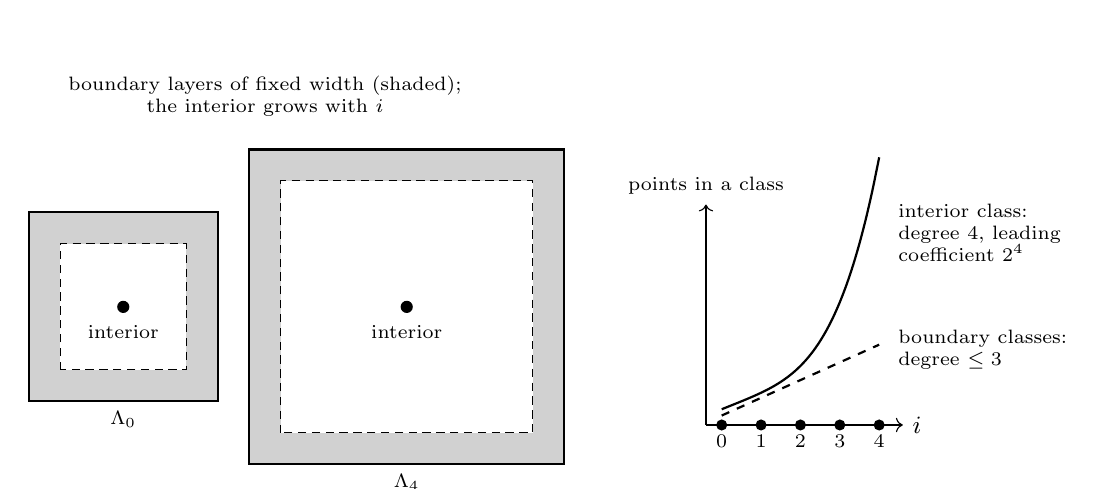
\begin{tikzpicture}[x=0.2cm,y=0.2cm,font=\small]
\foreach \h/\xs/\lab in {6/0/{$\Lambda_0$},10/18/{$\Lambda_4$}}{
  \begin{scope}[xshift=\xs*0.2cm]
  \fill[black!18] (-\h,-\h) rectangle (\h,\h);
  \fill[white] (-\h+2,-\h+2) rectangle (\h-2,\h-2);
  \draw[thick] (-\h,-\h) rectangle (\h,\h);
  \draw[densely dashed] (-\h+2,-\h+2) rectangle (\h-2,\h-2);
  \fill (0,0) circle (2.2pt);
  \node[font=\scriptsize] at (0,-1.6) {interior};
  \node[font=\scriptsize,below] at (0,-\h) {\lab};
  \end{scope}
}
\node[font=\scriptsize,align=center] at (9,13.4) {boundary layers of fixed width (shaded);\\ the interior grows with $i$};
\begin{scope}[xshift=7.4cm,yshift=-0.3cm]
\draw[->] (0,-6) -- (0,8) node[above,font=\scriptsize]{points in a class};
\draw[->] (0,-6) -- (12.5,-6) node[right]{$i$};
\foreach \i in {0,...,4} \fill (2.5*\i+1,-6) circle (2pt) node[below]{\scriptsize$\i$};
\draw[thick,domain=0:10,smooth,variable=\u] plot ({\u+1},{-5+12*(\u/10)^4+0.4*\u});
\draw[thick,dashed,domain=0:10,smooth,variable=\u] plot ({\u+1},{-5.4+0.45*\u});
\node[align=left,font=\scriptsize,anchor=west] at (11.6,6.2) {interior class:\\ degree $4$, leading\\ coefficient $2^4$};
\node[align=left,font=\scriptsize,anchor=west] at (11.6,-1.2) {boundary classes:\\ degree $\le3$};
\end{scope}
\end{tikzpicture}
\caption{The five reflected tori $\Lambda_i$ of Lemma~\ref{lem:D-localization}, of sides $2(w+i)$, drawn for $i=0$ and $i=4$. A point $y$ is classified by its local fold slopes and distances, through the read radius $R$, from reflection faces; on healthy $N_{2\bar w}(x)$, the shifted configurations $V_{i,x-\phi_i(y)}$ give the same local formula within each class. Boundary classes have multiplicity of degree at most three in $i$; the combined interior multiplicity has degree four and leading coefficient $2^4$. The fourth difference cancels the boundary classes and retains the interior contribution. The tori are auxiliary domains, and the cancellation takes place in the sum, not term by term.}
\label{fig:D-five-tori}
\end{figure}

Write $f_a^0$ for a regular summand of the negative logarithm in~\eqref{eq:D-cluster}, including its coefficient. Keep the inherited terms of Lemma~\ref{lem:D-inherited} separately. Call a remaining term \emph{low-order} if it is a connected term with at most two polymers of at most two elementary factors each, every path atom having length at most $B$, with no incoming activity factor or large-field component, or a path term of length at most $B$. Low-order terms read only the prescribed path, the coupling and the addresses, not the values of the incoming activities. Fix an exhaustion of the low-order addresses by finite sets invariant under translations and signed permutations, and select the low-order terms in one of these sets. Its index and the truncation error $\varepsilon_{\rm tr}$ are fixed in the proof of Lemma~\ref{lem:D-preliminary}. Give an ordinary term the shares $p_{xa}=\mathbf1_{X_a}(x)/|X_a|$, and a path term the share $\mathbf1_{\{o_a\}}(x)$; these shares sum to one. Put $F_x=\sum_{a\ {\rm selected}}p_{xa}f_a^0$, the selected low-order sum. The remaining terms form $f^{\rm tail}$. Let $R\ge1$ contain every complete read support of this finite sum relative to a site receiving a nonzero share, including all links read by its flag tests. The period argument below requires $R$ to be bounded by a fixed stage multiple of $1+B$ for the actual selected panel. The low-order factor count alone does not establish this for inverse or determinant defect chains; their read widths remain part of the verification in Lemma~\ref{lem:D-cutoff-continuity}. Set $w=4R+100(1+B)$, $\bar w=w+5$, and let $\Lambda_i$ have side $2(w+i)$, $0\le i\le4$. Use the fold $\phi_i$ and reflected configuration $V_{i,x}$ defined above. Put
\begin{equation}\label{eq:D-five-weights}
\lambda_i=\frac{(-1)^i\binom4i}{2^4\,4!},\qquad
G_x(V)=\sum_{i=0}^4\lambda_i\sum_{y\in\Lambda_i}F^{(i)}_y(V_{i,x})\,.
\end{equation}
Here $F^{(i)}$ is the same finite local formula on the auxiliary torus, with its value at $1$ subtracted at each site. The mask discrepancy and the constant of the redistribution are
\begin{equation}\label{eq:D-mask-localization}
L_x=\sum_{a\ \text{selected}}p_{xa}h_{X_a}f_a^0-F_x(1)
-\sum_{i=0}^4\lambda_i\sum_{y\in\Lambda_i}
 h_{N_{\bar w}(x-\phi_i(y))}F^{(i)}_y(V_{i,x-\phi_i(y)}),
\qquad c=F_0(1)\,,
\end{equation}
The shift is the folded position $\phi_i(y)$, not a torus representative.

For the estimates below put $\mathfrak b=\refbeta_{m+1}$; $P_j$ has subpower growth.
\begin{lemma}[Finite-period localization]\label{lem:D-localization}
The function $G_x$ is local on $N_{\bar w}(x)$, and
\begin{equation*}
\sum_a h_{X_a}f_a^0
=c|\Lambda|+\sum_a h_{X_a}f_a^{\rm tail}
+\sum_xh_{N_{\bar w}(x)}G_x+\sum_xL_x\,.
\end{equation*}
Each $L_x$ reads only links and flags in $N_{2\bar w}(x)$ and vanishes when that set is healthy, and
\begin{equation*}
\|G_x\|_{m,N_{\bar w}(x)}\le P_j(\mathfrak b)(\mathfrak b^{-23/20}+\varepsilon_{\rm tr}),
\qquad \sup|L_x|\le P_j(\mathfrak b)\mathfrak b^{-7/16}.
\end{equation*}
\end{lemma}
\begin{proof}
The identity is a rearrangement; the vanishing of $L_x$ is the fourth-difference cancellation; the bound on $G_x$ comes from the auxiliary logarithm, estimated with the classical and one-loop subtractions of Section~\ref{sec:partII-C}. For each $i,y$, translation by $\phi_i(y)$ is a bijection of the physical torus. Summing~\eqref{eq:D-mask-localization} over $x$ and changing $x$ to $x-\phi_i(y)$ gives exactly the asserted identity, including its masks. Translation symmetry makes $F_x(1)$ independent of $x$.

Use the polynomial period requirement in item~7 of Table~\ref{tab:constant-choices}, in addition to $100(B+1)\le L_pD_m$. Write $n=L_pD_m$. Subject to the stated stage-dependent bound on the actual read radius, $\bar w=4R+100(1+B)+5$ is bounded by a stage multiple $\bar a B/2$. The chosen stage has integers $v_j^{\rm per},h_j^{\rm per}$ with $v_j^{\rm per}\ge\bar a$, $h_j^{\rm per}\ge1$ and
\begin{equation*}
n\ge v_j^{\rm per}(1+B_m+B_{m+1})^{h_j^{\rm per}}.
\end{equation*}
These are the minimum-period choices made after the ratios. Since $B\ge1$,
\begin{equation*}
2\bar w\le\bar aB<\bar a(1+B_m+B_{m+1})^{h_j^{\rm per}}\le n,
\qquad 4R+16<n.
\end{equation*}
The reflection cubes, whose side is at most $2(w+4)<2\bar w$, therefore embed, as does every radius-$R$ read set. The larger health set $N_{2\bar w}(x)$ is a set on the original torus and need not embed; the argument uses only its containment of the queried links and flags.

For the local comparison, suppose that the field is healthy on the radius-$R$ neighbourhood. Translate its cube to $[0,2R]^4$. On integer representatives $0\le k<n$, fold each coordinate by $q(k)=k$ for $k\le2R$, $q(k)=4R-k$ for $2R<k\le4R$, and $q(k)=0$ thereafter. Pull back links along this map, reversing them on decreasing edges and setting them to the identity on collapsed edges. A plaquette becomes a plaquette of the original cube, with possible reversal and conjugation, or has identity holonomy. The field is therefore globally healthy and agrees with the original field on the cube. The bound $4R<n$ permits the construction without a divisibility assumption on $n$. Locality then permits this replacement when comparing the common local formulas on different periods.

We verify the vanishing of $L_x$ on a healthy $N_{2\bar w}(x)$. The complete read supports then lie in that set and every mask in~\eqref{eq:D-mask-localization} is one. At a site $y+u$ in the complete read, $\|u\|_\infty\le R$, the shifted reflected field reads the offset $\phi_i(y+u)-\phi_i(y)$ from~$x$, with inverse links on decreasing segments. This local profile depends only on the slope and on distances from the turning faces, including wrapped neighbours. Assign points at distance strictly less than $R$ from a face to boundary classes; each fixed boundary profile has a count independent of $i$. For each interior slope in one coordinate there are $h_i-2R+1$ sites with $R\le\phi_i(y)_a\le h_i-R$; there are two slopes. Multiplying the coordinate counts, every class meeting a boundary has multiplicity of degree at most three, while the combined interior multiplicity has leading coefficient $2^4$. Signed-permutation invariance identifies the values of the $2^4$ interior slope classes with $F_x(V)-F_x(1)$. The fourth difference therefore cancels all boundary classes and retains this value with coefficient one, proving $L_x=0$. Each shifted mask reads within $N_{2\bar w}(x)$ because $\|\phi_i(y)\|_\infty\le w+4<\bar w$.

\emph{Classification of the terms.} Here are the quantitative estimates on the sum before this localization. Put $\mathfrak b=\refbeta_{m+1}$ and $\mathfrak h=\mathfrak b^{3/8}$. In the convergent connected sums multiply the majorant of each ordinary elementary factor by $\mathfrak h$. The rooted attachment parameter still tends to zero, since $\mathfrak h \mathfrak b^{-7/16}=\mathfrak b^{-1/16}$. A term with at least three such factors across its polymers gains $\mathfrak h^{-3}$ upon restoring its original weights. A term with a retained large-field overlap has the same gain because its suppression is at least $\mathfrak h^{-3}$. The sum after multiplication has size at most a subpower factor times $\mathfrak h \mathfrak b^{-7/16}$. Thus the terms in these two classes have bound
\begin{equation}\label{eq:D-height-gain}
P_j(\mathfrak b)\mathfrak h^{-3}(\mathfrak h \mathfrak b^{-7/16})=P_j(\mathfrak b)\mathfrak b^{-19/16}
\le \mathfrak b^{-23/20}
\end{equation}
after the coupling threshold is raised. The reserve is $19/16-23/20=3/80$. This estimate also bounds fixed ordered derivatives: their placement polynomial was included before the rooted sum.

The connected sum separates into three parts. First retain the inherited terms using Lemma~\ref{lem:D-inherited}; their principal sum is made smaller than a prescribed multiple of $\epsilon^{\rm pre}_m$ by choosing the ratio, and their comparison remainder by raising the threshold. Among all other connected terms retain also those whose total support size exceeds the low-order radius: their support decay is at most $\mathfrak h^{-3}$ after the threshold is raised, so the estimate in~\eqref{eq:D-height-gain} applies to them. A term with an incoming regular factor and at least one further factor is not low-order. The rooted clause of Lemma~\ref{lem:D-connected}, with $W_\star$ that factor and at least one attached factor, bounds these terms by $P_j(\mathfrak b)\epsilon_{m+1}^{\rm reg}\mathfrak b^{-1/2}\le\mathfrak b^{-23/20}$. The remaining terms are low-order: the selected connected contributions and path terms of length at most $B$, to which the reflected-period construction is applied, and the low-order tail, of weighted norm at most $\varepsilon_{\rm tr}$. Long paths have an additional factor $e^{-w^{\rm path}_{J_m}B/4}$ by Lemma~\ref{lem:C1}; it converts their $\mathfrak b^{-7/16}$ bound to $\mathfrak b^{-23/20}$. Low-order connected terms with three or four elementary factors already obey~\eqref{eq:D-height-gain}; the remaining connected terms have at most two.

\emph{The auxiliary logarithm.} For the finite sum use the stationary integral on each $\Lambda_i$. Their sides $2(w+i)$ satisfy $2(w+i)\ge100(B+1)$. The entry choice $B\ge j+4$ also gives $\ell_m\,2(w+i)\ge100((j+3)\ell_m+1)$ for their fine periods. Thus the coarse-period form of Lemmas~\ref{lem:B-D1}--\ref{lem:B-D2} applies, without requiring these auxiliary periods to belong to the chosen physical-volume sequence. Subtract its flat value and the classical cubic, quartic and quadratic one-loop terms of Lemmas~\ref{lem:C4}--\ref{lem:C7}. Differentiation of its logarithm gives connected expectations under the common Gaussian law. For the terms not involving incoming errors, write the normalized local integral as $\mathbb E\exp(V_3+V_4+V_{\ge5})$, after the stationary action and its Gaussian determinant have been extracted. The subscripts refer to the Taylor degree in the link chart. Gaussian parity removes a lone odd cubic term. The fourth-order stationary terms are already in the classical path action, and the field-dependent quadratic part of the determinant is already in $\alpha\mathcal Q_m$ and the quadratic loop atoms. Subtracting the value at $1$ removes the remaining vacuum terms. Expanding $\log\mathbb E e^V$ through two factors gives $\mathbb EV+\frac12(\mathbb EV^2-(\mathbb EV)^2)$; its remaining terms have at least three factors. In normalized fluctuation coordinates each nonquadratic factor starts at order $\mathfrak b^{-1/2}$. The common Gaussian majorant bounds the last terms by $P_j(\mathfrak b)\mathfrak b^{-3/2}$. In the one- and two-factor terms that remain after the stated cancellations, Taylor's integral remainder and the healthy field bound give
\begin{equation*}
P_j(\mathfrak b)\{\mathfrak b^{-3/2}+\mathfrak b\,t_m^5+\mathfrak b^{-1}t_m+t_m^3+e^{-c_jB}\}
\le \mathfrak b^{-23/20}\,.
\end{equation*}
Every radius and chart loss is included in the subpower factor. Each of the four power terms has exponent at most $-3/2$ before that factor; the path exponential decreases faster than any fixed power. The quadratic subtraction uses the infinite-volume path coefficients, whereas the auxiliary logarithm uses the actual finite stationary branch. \hyperref[par:C-finite-period]{The finite-period recording paragraph} compares precisely these finite and periodized inputs. For $n_i=2(w+i)$ write its ordered-derivative error as
\begin{equation*}
\mathfrak e_i=C_{j,\ell_m}(1+\Lambda_{m+1}^{\rm loop})n_i^4P_{j,\ell_m}(n_i,B)e^{-c_{j,\ell_m}n_i}.
\end{equation*}
For the chart on the reflected configurations, choose paths from the origin in increasing coordinate order and gauge each bond by the paths to its endpoints. Commute a bond past the higher-coordinate path segments using at most $3(n_i-1)$ plaquette interchanges. A nonwrapping bond then cancels; for a wrapping bond the remaining coordinate cycle is the identity because the reflected extension traverses its links and then their reverses. Thus the gauge-fixed link chord is $O(n_it_m)$. Reflected perturbations retain the retracing property. Evaluate the exact gauge-invariant auxiliary functional and path subtraction in this smoothly chosen gauge before taking their flat Taylor expansions; the isolated quadratic expression in logarithms need not itself be invariant under a finite gauge change. Products of $O(n_i)$ links and the logarithm on a fixed ball around the identity have fixed-order derivatives bounded by a polynomial in $n_i$ and $B$. This construction concerns the auxiliary reflected configurations, not arbitrary healthy fields on a torus.

Here $P_{j,\ell_m}$ is a fixed polynomial for the ordered link derivatives and logarithmic-coordinate chain rules through the norm's prescribed order. The $n_i^4$ already bounds the whole torus quadratic form; no further site-count factor is applied to this error. Its flat value is zero, so centering leaves the quadratic difference unchanged. Differences between the nonlinear path representatives and their quadratic Taylor terms belong instead to the higher Taylor remainder displayed above. The comparison depends on the common analytic strip and its integrable bounds in \hyperref[par:C-finite-period]{the finite-period recording paragraph}; it also requires the reflected healthy torus to admit the coordinate charts and derivative bounds used for those chain rules. Both points remain under verification. At the fixed ratio, the stated bound on $n_i$ makes $\mathfrak e_i$ smaller than any prescribed inverse power of $\mathfrak b$. Terms involving incoming activities are not low-order; apart from the inherited terms they obey~\eqref{eq:D-height-gain} or the bound $P_j(\mathfrak b)\epsilon_{m+1}^{\rm reg}\mathfrak b^{-1/2}$ above. Subject to that finite-period comparison, Lemma~\ref{lem:B-D2} bounds these terms simultaneously, so the derivative bound for the centered total auxiliary sum is
\begin{equation}\label{eq:D-aux-bound}
C_j \mathfrak b^{-23/20}+\mathfrak e_i+2|\Lambda_i|\{C_j \mathfrak b^{-23/20}+\varepsilon_{\rm tr}\}\,.
\end{equation}
Here $\varepsilon_{\rm tr}>0$ is the chosen truncation error. The first term is the centered local integral, $\mathfrak e_i$ is the finite-period quadratic mismatch, and the two volume terms bound the omitted regular sum at the field and at $1$. Approaching a boundary point of the healthy domain by radial contraction preserves these estimates, so they hold on the closed domain used in Definition~\ref{def:D05a}.

A direction of that definition, restricted to $N_{\bar w}(x)$ and reflected, is bounded by $2t(1+\bar w)^{\varpi_{J_m}}$. Rescaling each of at most $\mathfrak q_{J_m}$ directions in~\eqref{eq:D-aux-bound} therefore gives
\begin{equation*}
\|G_x\|_{m,N_{\bar w}(x)}\le
2^{\mathfrak q_{J_m}}(1+\bar w)^{\varpi_{J_m}\mathfrak q_{J_m}}
\sum_{i=0}^4|\lambda_i|
 [C_j \mathfrak b^{-23/20}+\mathfrak e_i+2|\Lambda_i|(C_j \mathfrak b^{-23/20}+\varepsilon_{\rm tr})]\,.
\end{equation*}
All the factors outside the negative powers are fixed powers of $1+B$. Also $\cover_B(N_{\bar w}(x))$ is bounded by a stage constant. The regular bound divided by $\epsilon_m^{\rm reg}$ tends to zero, since $23/20>11/10$. Finally,~\eqref{eq:D-mask-localization} and the uncentered $\mathfrak b^{-7/16}$ bound give $\sup|L_x|\le P_j(\mathfrak b)\mathfrak b^{-7/16}$, with the same polynomial read radius. These logarithmic corrections tend to zero in the site norm at exponent $\sigma+2$ and vanish on healthy supports. Subject to the stated finite-period and sector inputs, these estimates give the bounds claimed for the localization.
\end{proof}

To specify the small coefficient, let $C_j^{\rm sub}$, $C_j^{\rm low}$ and $C_j^{\rm high}$ be the operator bounds for local subtraction, low path replacement and the part of high path replacement proportional to $\epsilon^{\rm pre}_m$. These are the three linear operations in the following subsections; they are fixed from the output derivative norm and path bounds. Put $C_j^0=C_j^{\rm sub}+C_j^{\rm low}+C_j^{\rm high}$. These constants use only derivative orders, direction powers, support exponents, and the output path bounds. For a prescribed $0<\theta\le1$, choose before the ratios
\begin{equation*}
c_j=\frac1{64(1+C_j^0)},\qquad \epsilon^{\rm pre}_m=\theta c_j\epsilon_m^{\rm reg}\,.
\end{equation*}
The quantity $\epsilon^{\rm pre}_m$ depends on $m$ through $\epsilon_m^{\rm reg}$. The next assertion concerns the very same block integral and the masks of~\eqref{eq:D-low-sums}. Its forced sum $\mathcal F_u^0$ is the disjoint-support exact-cover sum of Definition~\ref{def:D06} formed from the $k_{i,u}$, and $\mathfrak e_{i,u}\ge\|f_{i,u}\|_{m,X_i}$, $\mathfrak k_{i,u}\ge\sup_U|k_{i,u}(U)|$ are majorants.
\begin{lemma}[Preparatory activities]\label{lem:D-preliminary}
For every input curve above there are a continuous scalar $\tau_u$, local regular functions $f_{i,u}$, with the regularity of Definition~\ref{def:D24} before flat-value and Hessian subtraction, and forced activities $k_{i,u}$ (Definition~\ref{def:D25}), all with fixed addresses, equivariant and continuous in the weighted norms with exponents $\sigma+3$ and $\sigma+1$, such that
\begin{align}\label{eq:D-early}
\mathcal H_u(U)&=e^{\tau_u|\Lambda|-\beta'_u\mathsf K_m^{\rm kin}(U)-\mathcal L_m(U)
-\alpha_{N,m}\mathcal Q_m(U)-\sum_i h_{X_i}(U)f_{i,u}(U)}\mathcal F_u^0(U),\\
\sup_x\sum_{o_i=x}e^{(\sigma+3)\cover_B(X_i)}\mathfrak e_{i,u}&\le\epsilon^{\rm pre}_m,\label{eq:D-early-bound}\\
\sup_x\sum_{i:x\in Y_i}e^{(\sigma+1)\cover_B(Y_i)}\mathfrak k_{i,u}&\le e^{-\kappa_j^{\rm pre}(\cutoffsize_{m+1})^2},
\label{eq:D-preliminary-forced}
\end{align}
with $\kappa_j^{\rm pre}>0$ fixed after the ratio. Restricting the interval preserves all this.
\end{lemma}
\begin{proof}
The connected expansion of Lemma~\ref{lem:D-connected} supplies the terms, Lemma~\ref{lem:D-inherited} and the classification in the proof of Lemma~\ref{lem:D-localization} bound all but the low-order ones, and Lemma~\ref{lem:D-localization} localizes the latter; the choices below split $\epsilon^{\rm pre}_m$ among them. First choose the ratio so that the inherited principal terms of Lemma~\ref{lem:D-inherited} use at most $\epsilon^{\rm pre}_m/32$, and then raise the threshold so that their comparison remainders use at most $\epsilon^{\rm pre}_m/32$. Bound the terms retained in~\eqref{eq:D-height-gain} and the long paths together by $\epsilon^{\rm pre}_m/16$. The localization bound is $o(\epsilon^{\rm pre}_m)$ with the stronger support exponent. This fixes a coupling threshold independent of the period.

Next fix the truncation index. The low-order tail reads only the prescribed path, the coupling and the incoming addresses. For each coupling in $\mathfrak B_{m+1}$ summability gives a tail smaller than $\varepsilon_{\rm tr}/2$; weighted continuity in the coupling gives a neighbourhood on which the same tail is smaller than $\varepsilon_{\rm tr}$. Finitely many neighbourhoods cover the compact $\mathfrak B_{m+1}$; take the largest index. This argument gives an index for a fixed prescribed path and address lists. The cutoff comparison requires additional uniform control of the actual selections, including defect-chain tails, as specified in Lemma~\ref{lem:D-cutoff-continuity}. Increasing a valid index preserves its tail bound. Choose the tail bound to be at most $\epsilon^{\rm pre}_m/16$. The regular terms outside the finite sum then have total at most $(1/16+2/16)\epsilon^{\rm pre}_m$. Choose $\varepsilon_{\rm tr}$ so that the two localization errors in~\eqref{eq:D-aux-bound}, including the direction and support losses, have total at most $12\epsilon^{\rm pre}_m/16$. The resulting bound is $15\epsilon^{\rm pre}_m/16<\epsilon^{\rm pre}_m$.

The change in the scalar is $\tau_u^{\rm old}-F_0(1)$, with the sign fixed by~\eqref{eq:D-mask-localization}. Multiply the preliminary forced sum by $\exp(-\sum_xL_x)$. Expand each $e^{-L_x}$ about one and collect intersecting supports, as in the proof of Lemma~\ref{lem:D-fusion}. The logarithmic factors vanish unless their supports contain flags, so each resulting connected component still contains a forced term. Their site bound at exponent $\sigma+2$ is a subpower factor times $\mathfrak b^{-7/16}$, whereas each forced component retains $C_j e^{-r_j\beta'_u t_{m+1}^2}$. Choose a smaller positive $r'_j<r_j$. The site attachment parameter tends to zero and the remaining exponential gives
\begin{equation*}
C'_j e^{-r'_j\beta'_u t_{m+1}^2}
\le e^{-\kappa_j^{\rm pre}(\cutoffsize_{m+1})^2}
\end{equation*}
for some $\kappa_j^{\rm pre}>0$, since $\beta'_u\ge\refbeta_{m+1}/2$. One extra support power is used in this collection, leaving $\sigma+1$. Lemma~\ref{lem:D-rooted} proves the asserted site bound and absolute convergence. No scalar depends on the output configuration, and all identities hold also when a chord is exactly at a threshold.

For continuity, the truncation and all reflected tori are now fixed. Finite linear combinations preserve the weighted comparison from Lemma~\ref{lem:D-connected}. A difference of forced products has one marked difference factor; the rooted sum has the same strict attachment margin. Dominated convergence proves the weighted comparison after the collection. Flat evaluation gives continuity of the scalar. The support enlargement, inventories and conjunctions of tests are fixed. The same constructions commute with translations and signed permutations by reindexing. Every assertion is pointwise in the interval parameter or a convergence assertion within the interval, so restriction to a closed subinterval preserves it.
\end{proof}


The preparatory regular sum is $E_u^{\rm pre}=\sum_i f_{i,u}$ on the healthy domain. Its weighted bound is the anchored sum of Definition~\ref{def:D05b}, before flat-value and Hessian subtraction. The next identity supplies the scalar reset.

\begin{lemma}[Pre-reset expansion]\label{lem:D4}
For every input curve above and every $u$, there is a preparatory regular family with sum $E_u^{\rm pre}$ and weighted bound $\epsilon_m^{\rm reg}$ such that, when $\flags_m(U)=\varnothing$,
\begin{equation*}
\mathcal H_u(U)=\exp\{\tau_u|\Lambda|-\beta'_u\mathsf K_m^{\rm kin}(U)
-\alpha_{N,m}\mathsf K_{2,m}^{\rm kin}(U)-\mathcal L_m(U)-E_u^{\rm pre}(U)\}\,.
\end{equation*}
In particular $\mathcal H_u(1),\mathcal H_u(U)>0$ on this set.
\end{lemma}

\begin{proof}
Restrict the identity~\eqref{eq:D-early} to configurations without flags. Set $E_u^{\rm pre}=\sum_i f_{i,u}$ on configurations without flags. Every health mask is one, and nonempty forced inventories give $\mathcal F_u^0=1$. Equation~\eqref{eq:D-low-sums} gives $\mathcal Q_m=\mathsf K_{2,m}^{\rm kin}$. Dropping the extra three support powers gives the stated bound, since $\theta c_j\le1/64$. Absolute convergence makes the exponent finite and real, proving positivity, including at $1$. 
\end{proof}

\subsection{Local quadratic subtraction}\label{subsec:D-subtraction}

The subtraction is local and uses no bound on the eventual coupling correction. It extracts from each preliminary regular function its response to constant curls, written with the clover curvature of~\eqref{eq:D-clover-linear}.

For a preliminary $f$ on $X$ anchored at $o$, put $Z=X\cup N_2(o)$. For $q=(a,b)$ and $T\in\g$, set $A^{q,T}_{(y,c)}=\mathbf1_{c=b}\xi_o(y)^aT$, and fix a unit vector $T_*\in\g$. Define
\begin{align*}
q_f(q,r)&=D^2[f(\exp\cdot)](0)[A^{q,T_*},A^{r,T_*}],\\
Q_f(U)&=\frac12\sum_{q,r}q_f(q,r)\langle F^{\rm cl}_q(U,o),F^{\rm cl}_r(U,o)\rangle_{\g}\,.
\end{align*}
Set $q_f=0$ when $Z$ wraps. The matrix extracts the response to constant curls; its color independence is proved below. Define the regular remainder and the discrepancy of masks by
\begin{align}\label{eq:D-local-split}
R_f&=f-f(1)-Q_f,\notag\\
\zeta_f&=\mathbf1_{Z\,\mathrm{unhealthy}}\{f(1)+h_{\{o\}}Q_f-h_Xf\}\,.
\end{align}
The following identity is checked before any activities are summed.

\begin{lemma}[Local subtraction]\label{lem:D-local-subtraction}
For every preliminary regular $f$,
\begin{equation*}
h_Xf=f(1)+h_{\{o\}}Q_f-\zeta_f+h_ZR_f\,.
\end{equation*}
The function $R_f$ is regular on $Z$, vanishes at $1$, and has zero affine Hessian when $Z$ is nonwrapping. The Borel gauge-invariant function $\zeta_f$ depends only on internal links and flags in $Z$ and vanishes when $Z$ is healthy.
\end{lemma}

\begin{proof}
Gauge invariance reduces the affine Hessian to its response to constant curls, Schur's lemma makes that response colour-independent, and the clover formula~\eqref{eq:D-clover-linear} reproduces it. The first derivative of $f$ at the flat field vanishes: constant gauge transformations make its coefficient on each internal link an adjoint-invariant vector of $\g$, hence a central vector, which is zero. Differentiating local gauge invariance again makes its Hessian annihilate an infinitesimal gradient in either argument. On a nonwrapping support an affine field with zero curl is a local gradient. Its constant and symmetric linear parts are differences of a quadratic site field, with a constant adjustment for the discrete difference. Multiply this site field by a periodic cutoff equal to one on $Z$. The internal links read by $f$ are unchanged. The second differentiation of gauge invariance uses $Df(1)=0$, as proved above, so no second derivative of the gauge orbit remains. Hence the affine Hessian depends only on the constant curls.

For each pair of orientations the colour form $(S,T)\mapsto D^2[f(\exp\cdot)](0)[A^{q,S},A^{r,T}]$ is $\operatorname{Ad}(G)$-invariant. The complexified adjoint representation of the compact simple Lie algebra $\g$ is irreducible, so every invariant bilinear form on $\g$ is a multiple of the trace form (Schur's lemma); testing on $T_*$ identifies the multiple.

The side satisfies $L_pD_m\ge100(B_m+1)>20$, which permits the clover loops and affine tests without degeneracies. Equation~\eqref{eq:D-clover-linear} identifies the affine Hessian of $Q_f$ with that of $f$. Subtracting gives zero diagonal affine Hessian for $R_f$; polarization gives zero on pairs. The value and first derivative of $R_f$ vanish at $1$. If $Z$ wraps, no Hessian cancellation is required. The clover polynomial is smooth, Borel, gauge invariant and local on $N_2(o)$, which gives the other regularity assertions on $Z$.

All indicators in $\zeta_f$ read flags in $Z$. If $Z$ is healthy, every mask in the identity is one and $\zeta_f=0$; the identity reduces to the definition of $R_f$. If $Z$ is unhealthy, $h_ZR_f=0$ and the definition of $\zeta_f$ gives the identity directly. This proves the equality on every configuration and the stated locality and cancellations.
\end{proof}

The same subtraction has a quantitative bound. If $a_f$ majorizes $f$, the diagonal tests $tA^{q,T_*}$ and their half-sum are permitted directions in Definition~\ref{def:D05a}. They give
\begin{equation}\label{eq:D-projection-bound}
t^2|q_f(q,q)|\le a_f,\qquad t^2|q_f(q,r)|\le3a_f\,.
\end{equation}
Indeed four times the half-sum's diagonal Hessian is $t^2(q_f(q,q)+q_f(r,r)+2q_f(q,r))$. Its absolute value and the two diagonal bounds give the second estimate. Product differentiation of the four-link formula bounds every permitted derivative of $F^{\rm cl}_q$ by $C_jt$ at a healthy anchor. For order zero this follows from the plaquette chord bound; at positive order the direction factors supply $t$, and all undifferentiated group matrices are bounded. Hence
\begin{equation}\label{eq:D-remainder-bound}
\|R_f\|_{m,Z}+\sup_U|\zeta_f(U)|\le C_j a_f\,.
\end{equation}
For $\zeta_f$, the terms $Q_f$ and $f$ occur only under their own relaxed threshold tests, so the estimates still apply when $Z$ is unhealthy.

Enlargement satisfies $\cover_B(Z)\le\cover_B(X)+1$: one radius-$B$ ball centered at $o\in X$ contains $N_2(o)$ and meets the original connected cover. Also $\operatorname{dist}(x,o)\le C B\cover_B(Z)$ for $x\in Z$, by following the connected cover. For a support of covering number $n$ through $x$, its anchor lies within distance $C Bn$ of $x$, giving at most $C(1+B)^4(1+n)^4$ possible anchors. The inequality $(1+n)^4\le C e^n$ converts exponent $\sigma+3$ at the anchor to exponent $\sigma+1$ at a site: one support power bounds this polynomial and one remains unused. At exponent $\sigma$ the enlargement itself contributes only a stage constant. Without these extra powers the conversion would leave a polynomial in $n$ at the original exponent.

Sum $q_{f_{i,u}}$ at each anchor. Translation covariance makes the result independent of the anchor. Reflection in an axis belonging to exactly one of two distinct orientations changes the sign of the off-diagonal entry, so that entry is zero. Permuting axes identifies the diagonal entries. Thus a single real $\Delta_u$ satisfies
\begin{align}\label{eq:D-isotropy}
\sum_{o_i=o}q_{f_{i,u}}(q,r)&=\Delta_u\delta_{qr},\notag\\
\sum_i h_{\{o_i\}}Q_{f_{i,u}}
&=\frac{\Delta_u}2\sum_o h_{\{o\}}\sum_q|F^{\rm cl}_q(U,o)|^2\,.
\end{align}
The coefficient sums converge absolutely by~\eqref{eq:D-projection-bound}, and $t^2|\Delta_u|\le\epsilon^{\rm pre}_m$. In particular $|\Delta_u|\le\epsilon^{\rm pre}_m/t_m^2=\theta c_j\refbeta_m^{-1/10}(\cutoffsize_m)^{-2}<1$, since $\theta c_j\le1/64$, $\refbeta_m>1$ and $\cutoffsize_m\ge1$. This is already the numerical reset bound, and with Lemma~\ref{lem:C7} it gives the drift bound of Lemma~\ref{lem:C8} directly; no further restriction enters. The probe argument in the proof of Lemma~\ref{lem:C8} is a second proof of $|\Delta_u|\le1$ with a separate role: it reads $\Delta_u$ off the two numbers $\mathcal H_u(1),\mathcal H_u(V)$ as the unique root of an affine equation, without the formula~\eqref{eq:D-isotropy}. Hence no other coupling correction fits the same activities, and $\Delta_u$ is continuous in~$u$ because the block integral and the activity sums are (Lemma~\ref{lem:D6}).

\subsection{Forced fusion, activity bounds and the reset}\label{subsec:D-fusion}

Put $\alpha=\alpha_{N,m}$. After Section~\ref{subsec:D-subtraction} the exponent contains $\alpha\mathcal Q_m+\frac{\Delta_u}2\sum_oh_{\{o\}}\sum_q|F^{\rm cl}_q(U,o)|^2$, whereas the output density must contain $(\alpha+\Delta_u)\mathsf K^{\rm kin}_m$. The difference consists of clover versus plaquette curvature, the missing cubic and quartic atoms, and the clips and health masks. The first two become regular activities, $e_{\lambda,u}$ below and $-(\alpha+\Delta_u)\mathfrak a^{(k)}_i$; the third, $\ell_{\lambda,u}$, vanishes on healthy supports and, with the mask discrepancies $\zeta_f$ of Lemma~\ref{lem:D-local-subtraction}, is absorbed into the forced activities by Lemma~\ref{lem:D-fusion}. Define
\begin{align}\label{eq:D-kinetic-split}
e_{\lambda,u}&=\Delta_u(L^{\rm cl}_\lambda-L^{\rm raw}_\lambda),\notag\\
\ell_{\lambda,u}&=(\alpha+\Delta_u)(L_\lambda-h_{Z_\lambda}L^{\rm raw}_\lambda)
+\Delta_u(h_{Z_\lambda}-h_{\{o_\lambda\}})L^{\rm cl}_\lambda\,.
\end{align}
The regular function is used with mask $h_{Z_\lambda}$. Its affine Hessian vanishes because its two terms have the same constant-curl response. Add also the regular cubic and quartic functions $-(\alpha+\Delta_u)\mathfrak a_i^{(k)}$, with their prescribed masks; they have zero Hessian because $k\ge3$. Every $\ell_{\lambda,u}$ vanishes on healthy $Z_\lambda$.

Write the logarithmic corrections $\zeta_{f_{i,u}}$ and $\ell_{\lambda,u}$ as $\ell_a$ on nonempty supports $Z_a$. A connected selection $P$ consists of preliminary forced labels and logarithmic labels, contains at least one forced label, and has pairwise disjoint preliminary forced supports. Connected means connected in the graph joining intersecting supports. Its support $Y_P$ is the union of all supports, including logarithmic supports; its inventory $I_P$ is the union of the preliminary forced inventories. Define
\begin{equation}\label{eq:D-fused-term}
K_P(U)=\mathbf1_{\{Y_P\cap\flags_m(U)=I_P\}}
\prod_{i\in P_{\rm for}}k_{i,u}(U)
\prod_{a\in P_{\rm log}}(e^{\ell_a(U)}-1)\,.
\end{equation}
The extra test is the conjunction of the preliminary forced tests. Selections and tests are fixed as $u$ varies.

\begin{lemma}[Forced fusion]\label{lem:D-fusion}
Suppose $\sum_a\sup_U|\ell_a(U)|<\infty$. For $\kappa_{\rm fus},\gamma\ge0$ assume nonnegative $v_a$ for all forced and logarithmic labels with
\begin{equation*}
|k_i|\le e^{-\kappa_{\rm fus}}v_i,\quad |e^{\ell_a}-1|\le v_a,\quad
\sup_x\sum_{a:x\in Z_a}e^{(\sigma+1)\cover_B(Z_a)}v_a\le\gamma,
\quad(2B+1)^4\gamma\le1\,.
\end{equation*}
Then the exact-cover gas of~\eqref{eq:D-fused-term} equals $\mathcal F_u^0\exp(\sum_a\ell_a)$ and its forced norm of Definition~\ref{def:D05b} is at most $e^{-\kappa_{\rm fus}}(e^\gamma-1)$.
\end{lemma}

\begin{proof}
The identity is a regrouping of finite selections into overlap components; the bound is Lemma~\ref{lem:D-rooted}. Expand $\exp(\sum_a\ell_a)=\prod_a(1+(e^{\ell_a}-1))$. Decompose a finite selection, together with a selection from $\mathcal F_u^0$, into support-overlap components. A nonzero logarithmic factor meets a flag. Exact coverage assigns that flag to a preliminary forced label, whose support meets the logarithmic support. Every component therefore contains a forced label. Their union supports are disjoint; their union inventories cover all flags. Conversely the components recover the original selection uniquely. The eligibility indicator in~\eqref{eq:D-fused-term} equals one on any such nonzero product: another component cannot supply a flag in $Y_P$, since its support is disjoint. This proves the identity for finite expansions.

For the absolute bound retain $e^{-\kappa_{\rm fus}}$ from one forced label per connected selection. Apply Lemma~\ref{lem:D-rooted}, with $\eta=1$, to the weights $\mathfrak v_i=v_ie^{\sigma\cover_B(Z_i)}$; its hypothesis follows from $(2B+1)^4\gamma\le1$ and the extra exponent in the hypothesis here. It bounds the rooted tree sums by $\mathfrak v_ie^{\cover_B(Z_i)}$, and the sum of these bounds over roots whose supports contain a fixed site is at most $\gamma$. Every connected selection has a spanning tree rooted at a label whose support contains that site, so its sum is at most $\gamma\le e^\gamma-1$. The covering number is subadditive on intersecting unions, which retains $e^{\sigma\cover_B(Y_P)}$ in this comparison. Restoring $e^{-\kappa_{\rm fus}}$ gives the claimed bound. The resulting summable envelope justifies passage from finite expansions to the infinite identity.
\end{proof}

Let $E_u^{\rm sum}$ be the masked sum of the $R_{f_{i,u}}$, the $e_{\lambda,u}$, and the cubic and quartic corrections. Let $\mathcal F_u$ be the fused gas. Hold these functions fixed while a trial parameter $\vartheta$ varies, and put
\begin{equation*}
q_{u,\vartheta}=e^{-(\beta'_u+\alpha_{N,m}+\vartheta)\mathsf K_m^{\rm kin}-\mathcal L_m-E_u^{\rm sum}}\mathcal F_u\,.
\end{equation*}
The parameter $\vartheta$ is the free coupling correction of the scalar reset. Lemma~\ref{lem:D5} shows that $\vartheta=\Delta_u$ gives the density identity at every configuration; at one healthy test configuration $V$ with $\mathsf K^{\rm kin}_m(V)>0$, Lemma~\ref{lem:C8} uses the affine dependence on $\vartheta$ to read off $\Delta_u$, which gives its continuity in $u$ and, with Lemma~\ref{lem:C7}, the drift bound.
The output representation is the following single list: regular addresses $(Z_i,o_i)$ with functions $R_{f_{i,u}}$, addresses $(Z_\lambda,o_\lambda)$ with functions $e_{\lambda,u}$, the cubic and quartic addresses of Definition~\ref{def:D22} with functions $-(\alpha+\Delta_u)\mathfrak a_i^{(k)}$, and forced addresses $(Y_P,I_P,\mathcal E_P^{\rm extra})$ with functions $K_P$. Each regular function carries its own health mask. We prove the inequalities
\begin{equation}\label{eq:D-fusion-small}
e^{-\kappa_{\rm fus}}(e^\gamma-1)\le\epsilon_m^{\rm for},\qquad
\mathcal E_m\le\epsilon_m^{\rm reg}\,.
\end{equation}
in Lemma~\ref{lem:D1} before using them for the density identity. They impose no condition on the trial coupling.

\begin{lemma}[Activity bounds and covariance]\label{lem:D1}
For every coarse output constructed above, both activity families are countable and equivariant under translations and $\hypercubic$, including supports, anchors, inventories and tests. There exist nonnegative majorants as in Definitions~\ref{def:D05a}--\ref{def:D05b} whose weighted series converge and which satisfy
\begin{equation*}
\mathcal E_m\le\epsilon_m^{\rm reg},\qquad
\mathcal K_m\le\epsilon_m^{\rm for}\,.
\end{equation*}
\end{lemma}
Lemma~\ref{lem:D3} states the same bounds for the Wilson representation, and Lemma~\ref{lem:D2} extends them to all the chosen classes.


\begin{proof}[Proof for a coarse output]
The regular bound adds the contributions of the three linear operations to the preparatory bound of Lemma~\ref{lem:D-preliminary}; the forced bound applies Lemma~\ref{lem:D-fusion}. Equation~\eqref{eq:D-remainder-bound} controls each subtracted function. The low regular terms are bounded by $C_j\epsilon^{\rm pre}_m$, since $t^2|\Delta_u|\le \epsilon^{\rm pre}_m$. The high terms are bounded by $C_j(|\alpha|t^3+\epsilon^{\rm pre}_m)$: each has at least three curvature factors, and $|\Delta_u|t^3\le \epsilon^{\rm pre}_mt\le \epsilon^{\rm pre}_m$. A derivative of a word of length $l$ introduces a fixed power of $1+l$, by the product rule and the allowed spatial growth of the directions. The support obeys $\cover_B(Z_\lambda)\le C+l/B$. Raise the threshold until $\sigma/B\le w^{\rm path}_{J_m}/4$. A quarter of the path exponent then bounds the support weight, and another quarter bounds this polynomial, since $\sup_{l\ge0}(1+l)^ke^{-wl/2}<\infty$. Summing Lemma~\ref{lem:C1} gives the previously defined constant $C_j^0$ and a constant $C_j^1$ with
\begin{equation*}
\mathcal E_m\le C_j^0\epsilon^{\rm pre}_m+C_j^1|\alpha|t^3\,.
\end{equation*}
The constant $c_j=[64(1+C_j^0)]^{-1}$ was chosen before the ratios in Lemma~\ref{lem:D-preliminary}. After the ratio is fixed, Lemma~\ref{lem:C7} bounds $|\alpha|$; raise the entry threshold until $C_j^1|\alpha|t^3\le\epsilon_m^{\rm reg}/2048$. This is possible because $t^3/\epsilon_m^{\rm reg}=\refbeta_m^{-2/5}(\cutoffsize_m)^3\to0$. Take $\theta\le1/32$ before the ratio. Since $C_j^0c_j\le1/64$, the sum is at most $\epsilon_m^{\rm reg}/1024$. The same argument allows any prescribed smaller coefficient by choosing $\theta$ first and raising the threshold for the second term.

For the logarithmic corrections, conversion from anchored sums to site sums introduces at most $C_j(1+B)^4$, after the extra support powers absorb the powers of the covering number. The local subtraction is bounded by $C_j\epsilon^{\rm pre}_m$. The low terms in~\eqref{eq:D-kinetic-split} are bounded by
\begin{equation*}
C_j(1+B)^4\{(|\alpha|+\epsilon^{\rm pre}_m/t^2)t+\epsilon^{\rm pre}_m\}=:m_j\,.
\end{equation*}
The linear clipped tail is bounded by $2c_{\rm lin}t$ times its coefficient, since chords are at most two. For a failed relaxed threshold test, the remote threshold supplies $e^{l/R_{J_m}^{\rm rel}}$ in a path of length $l$. The path decay absorbs it because $R_{J_m}^{\rm rel}w_{J_m}^{\rm path}\ge12$. The common-anchor clover term is bounded by $|\Delta_u|t^2\le \epsilon^{\rm pre}_m$. These estimates give exactly the displayed bound, including unhealthy configurations. Since $\epsilon^{\rm pre}_m/t=O_j(\refbeta_m^{-3/5}/\cutoffsize_m)$ and $|\alpha|$ is fixed after the ratio, $(1+B)^4m_j\to0$.

Let $\kappa_{\rm fus}=\kappa_j^{\rm pre}(\cutoffsize_{m+1})^2/2$. The majorants in~\eqref{eq:D-preliminary-forced}, multiplied by $e^{\kappa_{\rm fus}}$, have rooted total at most $e^{-\kappa_{\rm fus}}$. For each logarithm use $|e^{\ell_a}-1|\le2|\ell_a|$ once its individual majorant is at most $\log2$; this follows by increasing the entry threshold until $m_j\le\log2$. Their rooted total is at most $2m_j$. Increase the entry threshold so that $(2B+1)^4\gamma\le1/2$ for $\gamma=e^{-\kappa_{\rm fus}}+2m_j$. Lemma~\ref{lem:D-fusion} applies. Increase the threshold further so that $\gamma\le1$ and $e^{-\kappa_{\rm fus}}(e^\gamma-1)\le\epsilon_m^{\rm for}/1024$. Indeed $e^\gamma-1\le2\gamma$ and $\kappa_{\rm fus}\gg(\cutoffsize_m)^{1/5}$. This proves the forced inequality and summability in~\eqref{eq:D-fusion-small}.

Every address is a finite combination of countable preliminary and path addresses, so the families are countable. Subtraction and path replacement transport the entire address under translations. Signed permutations transform the curvature orientations with their signs; the finite group average includes every transformed term. These permutations act on supports, anchors and functions. On a connected selection they also transform the union inventory and conjunction of tests. Equation~\eqref{eq:D-fused-term} therefore has the required covariance. For an inverse link, $(e^{zA}U)^{-1}=e^{-z\operatorname{Ad}_{U^{-1}}A}U^{-1}$. Differentiating this identity repeatedly gives only finitely many product-rule terms through order $\mathfrak q_{J_m}$; the adjoint-invariant norm bounds them by a constant depending on that order. This proves the complete address covariance and the convergent weighted bounds for a coarse output. The Wilson start is established below; induction in Lemma~\ref{lem:D2} then gives the class assertion.
\end{proof}

The identity below fixes the whole density before the scalar estimate of Lemma~\ref{lem:C8}. Its proof uses the bounds just established.
\begin{lemma}[Exact density representation]\label{lem:D5}
The final activities satisfy Lemma~\ref{lem:D1}, vanish at the flat field in their regular part, and are independent of $\vartheta$. For every $u$ there is $\Delta_u\in\R$ such that
\begin{equation*}
q_{u,\Delta_u}(U)=\frac{\mathcal H_u(U)}{\mathcal H_u(1)}
\qquad\text{for every }U\,.
\end{equation*}
Moreover $\mathcal F_u(U)=1$ when $\flags_m(U)=\varnothing$. 
\end{lemma}

\begin{proof}
Local subtraction rewrites the preliminary regular functions, path replacement turns the masked quadratic functional into the kinetic action, and fusion absorbs the logarithmic corrections; the bounds~\eqref{eq:D-fusion-small} make every sum converge. Choose $\Delta_u$ by~\eqref{eq:D-isotropy} and put $c_u=\sum_i f_{i,u}(1)$. Local subtraction gives
\begin{equation*}
\sum_i h_{X_i}f_{i,u}=c_u+\frac{\Delta_u}2\sum_o h_{\{o\}}\sum_q|F^{\rm cl}_q|^2
-\sum_i \zeta_{f_{i,u}}+\sum_i h_{Z_i}R_{f_{i,u}}\,.
\end{equation*}
All sums converge absolutely. For each low term~\eqref{eq:D-kinetic-split} gives
\begin{equation*}
\begin{aligned}
&(\alpha+\Delta_u)L_\lambda+\Delta_u h_{Z_\lambda}(L^{\rm cl}_\lambda-L^{\rm raw}_\lambda)-\ell_{\lambda,u}\\
&\qquad=\alpha h_{Z_\lambda}L^{\rm raw}_\lambda+\Delta_u h_{\{o_\lambda\}}L^{\rm cl}_\lambda\,.
\end{aligned}
\end{equation*}
Sum and apply~\eqref{eq:D-low-sums}. The high corrections cancel $(\alpha+\Delta_u)\mathcal A_m$. Thus the exponent in~\eqref{eq:D-early} becomes
\begin{equation*}
\begin{aligned}
&(\tau_u-c_u/|\Lambda|)|\Lambda|
-(\beta'_u+\alpha+\Delta_u)\mathsf K_m^{\rm kin}-\mathcal L_m-E_u^{\rm sum}\\
&\qquad+\sum_i \zeta_{f_{i,u}}+\sum_\lambda\ell_{\lambda,u}\,.
\end{aligned}
\end{equation*}
Lemma~\ref{lem:D-fusion} incorporates the last two sums into $\mathcal F_u$. Hence, on every configuration,
\begin{equation}\label{eq:D-unnormalized}
\mathcal H_u(U)=e^{(\tau_u-c_u/|\Lambda|)|\Lambda|}q_{u,\Delta_u}(U)\,.
\end{equation}
At $1$ all path and final regular terms vanish. The only exact-cover forced selection is empty, so $q_{u,\vartheta}(1)=1$ for every $\vartheta$. Equation~\eqref{eq:D-unnormalized} proves the quotient identity and positivity of its denominator. The same empty-selection argument gives $\mathcal F_u=1$ whenever there are no flags.

The regular cancellations were proved in Lemma~\ref{lem:D-local-subtraction} and after~\eqref{eq:D-kinetic-split}; the weighted bounds are those of Lemma~\ref{lem:D1}. The value $\Delta_u$ used in the activity construction is already fixed by the preliminary functions. The trial variable $\vartheta$ occurs only in the exponential defining $q_{u,\vartheta}$. This proves the exact identity without using Lemma~\ref{lem:C8} or its reset estimate.
\end{proof}

\paragraph{The scalar reset.}\label{subsec:C-reset}

The density identity of Lemma~\ref{lem:D5} holds with a value $\Delta_u$ that the construction fixes before the bound on it proved here is used. The proof order is
\begin{equation*}
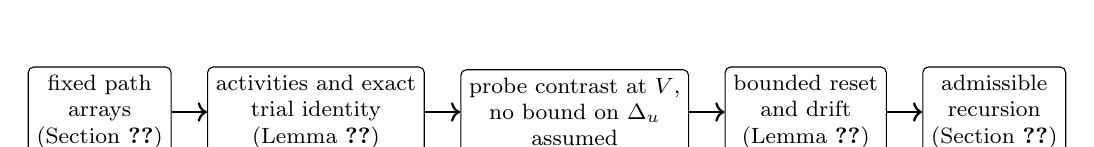
\begin{tikzpicture}[baseline=(c.base),node distance=0.45cm,every node/.style={draw,rounded corners=2pt,align=center,font=\footnotesize,inner sep=3pt}]
\node (a) {fixed path\\arrays\\(Section~\ref{sec:partII-C})};
\node[right=of a] (b) {activities and exact\\trial identity\\(Lemma~\ref{lem:D5})};
\node[right=of b] (c) {probe contrast at $V$,\\no bound on $\Delta_u$\\assumed};
\node[right=of c] (d) {bounded reset\\and drift\\(Lemma~\ref{lem:C8})};
\node[right=of d] (e) {admissible\\recursion\\(Section~\ref{subsec:D-recursion})};
\foreach \x/\y in {a/b,b/c,c/d,d/e} \draw[->,thick] (\x) -- (\y);
\end{tikzpicture}
\end{equation*}
Before the estimate below the following are available: the path arrays and $\alpha_{N,m}$ (Section~\ref{sec:partII-C}), the activity families with their bounds (Lemma~\ref{lem:D1}), and the exact identity $q_{u,\Delta_u}=\mathcal H_u/\mathcal H_u(1)$ (Lemma~\ref{lem:D5}). Section~\ref{subsec:D-subtraction} already gives $t_m^2|\Delta_u|\le\epsilon^{\rm pre}_m$, which the activity bounds use and which alone implies $|\Delta_u|<1$ and the drift bound. The estimate below is an alternative proof of $|\Delta_u|\le1$ that uses the activity bounds but not the formula for~$\Delta_u$. The reset gives a second description of the same coefficient: evaluating the identity at one configuration with positive kinetic energy identifies $\Delta_u$ as the unique root of an affine scalar equation. This explicit formula, with the continuity of Lemma~\ref{lem:D6} in Section~\ref{subsec:D-continuity} (whose proof does not use Lemma~\ref{lem:C8}), gives the continuity of $\Delta_u$ in $u$; with Lemma~\ref{lem:C7} it gives the drift bound.

For an input curve $\rho'_u$ of Theorem~\ref{prop:RG}, recall $\mathcal H_u=\blockmap{m}_{\beta'_u}\density\rho'_u$, and put $b_u=\beta'_u+\alpha_{N,m}$. Lemma~\ref{lem:D5} supplies regular and forced sums $E_u^{\rm sum},\mathcal F_u$, independent of $\vartheta$, with trial density
\begin{equation*}
q_{u,\vartheta}(U)=e^{-(b_u+\vartheta)\mathsf K^{\rm kin}_m(U)-\mathcal L_m(U)-E_u^{\rm sum}(U)}\mathcal F_u(U)\,,
\end{equation*}
the flat-field normalizations $q_{u,\vartheta}(1)=1$, and $q_{u,\Delta_u}=\mathcal H_u/\mathcal H_u(1)$. Lemma~\ref{lem:D4} gives a preparatory sum $E_u^{\rm pre}$ with bound $c_{\rm pre}\epsilon_m^{\rm reg}/4$, for a stage constant $c_{\rm pre}\ge4$, and Lemma~\ref{lem:D1} gives the final bound~\eqref{eq:I12-activity-caps}. The remaining scalar correction can be read from a single configuration with a definite kinetic energy.

\begin{lemma}[Coupling reset]\label{lem:C8}
For each input curve of Theorem~\ref{prop:RG}, take the families and real $\Delta_u$ supplied by Lemma~\ref{lem:D5}, with no bound on $\Delta_u$ assumed. Then $|\Delta_u|\le1$, and $\beta_u=\beta'_u+\alpha_{N,m}+\Delta_u$ is continuous and satisfies
\begin{equation*}
\beta_u=\beta'_u-\slope\log\ell_m+e_u,\qquad
|e_u|\le d_j+1\le\omega_j^{\rm RG}\,.
\end{equation*}
The bound is independent of $N,p,u$ and the input curve.
\end{lemma}

\begin{proof}
We evaluate the exact identity of Lemma~\ref{lem:D5} at one configuration $V$ with kinetic energy of order $|\Lambda|t_m^2$; the identity is affine in the reset, which is then read off. Recall $t=t_m\le1$ from item~7 of Table~\ref{tab:constant-choices}. Put a group element of chord $h_V=\tau t$ on direction-$1$ links whose second coordinate is even, and the identity elsewhere. Continuity along a nonconstant one-parameter subgroup gives $\varepsilon_G>0$ such that every chord in $[0,\varepsilon_G]$ occurs. Choose
\begin{equation*}
0<\tau\le\min\left(\varepsilon_G,\frac14,
\frac{c_{{\rm dir},J_m}}{512(1+A_{J_m}^{\rm path})}\right)\,.
\end{equation*}
Every $(1,2)$ plaquette has chord $h_V$ and all other plaquettes have chord zero. Thus this configuration~$V$ is everywhere healthy. All periods here are even because $4\mid L_p$. Signed permutations permute the plaquettes and preserve their chords, so the direct contribution to $\mathsf K^{\rm kin}_m(V)$ is at least $|\Lambda|c_{{\rm dir},J_m}h_V^2/2$. Row squares are nonnegative. Since $|\operatorname{proj}_{\g}(U-U^{-1})/2|\le\chord(U)$ and adjoint transport is isometric, every slot has norm at most $h_V\le1/4$. Lemma~\ref{lem:C1} bounds the absolute sum of cubic and quartic terms by
\begin{equation*}
2|\Lambda|A_{J_m}^{\rm path}h_V^3
\le |\Lambda|c_{{\rm dir},J_m}h_V^2/4\,.
\end{equation*}
Each signed image of~$V$ has the same plaquette chords with a single nonzero orientation. Hence the bounds apply to every term of the hypercubic average. Consequently
\begin{equation*}
K_V=\mathsf K^{\rm kin}_m(V)\ge|\Lambda|c_Vt^2,
\qquad c_V=c_{{\rm dir},J_m}\tau^2/4>0\,.
\end{equation*}

Lemma~\ref{lem:D4} gives $\mathcal H_u(1),\mathcal H_u(V)>0$. Put $v_u=|\Lambda|^{-1}\log \mathcal H_u(1)$. Taking the logarithmic contrast in Lemma~\ref{lem:D4} gives
\begin{equation}\label{eq:C-prereset}
\log\frac{\mathcal H_u(1)}{\mathcal H_u(V)}
=\beta'_u\mathsf K^{\rm kin}_m(V)+\alpha_{N,m}\mathsf K^{\rm kin}_{2,m}(V)
+\mathcal L_m(V)+E_u^{\rm pre}(V)-E_u^{\rm pre}(1)\,.
\end{equation}
The pre-reset bound of Lemma~\ref{lem:D4}, summed over anchors as in Definition~\ref{def:D05b}, bounds each of the last two values by $|\Lambda|c_{\rm pre}\epsilon_m^{\rm reg}/4$. No vanishing condition at~$1$ is needed for this preparatory sum.

On everywhere-healthy configurations every curvature slot has norm at most~$t$. Lemma~\ref{lem:C1} and $t\le1$ therefore give
\begin{equation*}
|\mathsf K^{\rm kin}_m-\mathsf K^{\rm kin}_{2,m}|\le2|\Lambda|A_{J_m}^{\rm path}t^3\,.
\end{equation*}
After $\ell$ is fixed, Lemma~\ref{lem:C7} bounds $|\alpha_{N,m}|$ by a stage constant. Raise the coupling entry threshold until $2|\alpha_{N,m}|A_{J_m}^{\rm path}t^3\le c_{\rm pre}\epsilon_m^{\rm reg}/2$. This is possible since $t^3/\epsilon_m^{\rm reg}=\refbeta_m^{-2/5}(\cutoffsize_m)^3\to0$. Together with~\eqref{eq:C-prereset} this yields
\begin{equation*}
\left|b_uK_V+\mathcal L_m(V)-\log\frac{\mathcal H_u(1)}{\mathcal H_u(V)}\right|
\le|\Lambda|c_{\rm pre}\epsilon_m^{\rm reg}\,.
\end{equation*}
For the final regular sum, Lemma~\ref{lem:D1} and~\eqref{eq:I12-activity-caps} give
\begin{equation*}
|E_u^{\rm sum}(V)|\le\sum_x\sum_{o_i=x}e_i^{\rm maj}
\le|\Lambda|\mathcal E_m\le|\Lambda|\epsilon_m^{\rm reg}\,.
\end{equation*}

Since the activity families are fixed as $\vartheta$ varies, the scalar discrepancy is affine:
\begin{align*}
f(u,\vartheta)&=(b_u+\vartheta)K_V+\mathcal L_m(V)+E_u^{\rm sum}(V)
-\log\frac{\mathcal H_u(1)}{\mathcal H_u(V)}\\
&=f(u,0)+\vartheta K_V\,.
\end{align*}
Since $V$ has no flagged sites, $\mathcal F_u(V)=1$. Evaluating the exact identity of Lemma~\ref{lem:D5} at $V$ gives $f(u,\Delta_u)=0$. As $K_V>0$, this determines
\begin{equation*}
\Delta_u=-f(u,0)/K_V,\qquad
|\Delta_u|\le\frac{(c_{\rm pre}+1)\epsilon_m^{\rm reg}}{c_Vt_m^2}\le1\,.
\end{equation*}
Increase the entry threshold to obtain the final inequality, using $\epsilon_m^{\rm reg}/t_m^2=\refbeta_m^{-1/10}(\cutoffsize_m)^{-2}\to0$. The block integral and activity sums are continuous in~$u$ by Lemma~\ref{lem:D6} of Section~\ref{subsec:D-continuity}, whose proof does not use the present lemma; so $\Delta_u$ is continuous.

Multiplication by $\mathcal H_u(1)=e^{v_u|\Lambda|}$ gives the density identity at~$\Delta_u$. Its coupling is $\beta_u=\beta'_u+\alpha_{N,m}+\Delta_u$. Lemma~\ref{lem:C7} and $|\Delta_u|\le1$ prove the claimed drift.
\end{proof}

\subsection{Continuity at fixed volume}\label{subsec:D-continuity}

The scalar reset of Lemma~\ref{lem:C8} and the step on curves need continuity of the integral and both final sums. The next deduction uses the weighted comparison in Lemma~\ref{lem:D-preliminary} and does not use Lemma~\ref{lem:C8}.

\begin{lemma}[Continuity of the activity sums]\label{lem:D6}
For input curves of Theorem~\ref{prop:RG}, the final activity families have fixed addresses and are continuous in the weighted sense of Definition~\ref{def:D25a}. For every fixed configuration $U$,
\begin{equation*}
u\longmapsto\mathcal H_u(U),\qquad
u\longmapsto E_u^{\rm sum}(U),\qquad
u\longmapsto\mathcal F_u(U)
\end{equation*}
are continuous.
\end{lemma}

\begin{proof}
Every operation of the step is linear at fixed addresses or a convergent product with a strict attachment margin, so the weighted continuity of Lemma~\ref{lem:D-preliminary} carries over. The maps $f\mapsto f(1),q_f,R_f,\zeta_f$ are linear on functions with fixed address. Equation~\eqref{eq:D-projection-bound} applied to a difference bounds its projection coefficients by its derivative majorant divided by $t^2$. Weighted preliminary continuity therefore gives continuity of $c_u$, $\Delta_u$, and the subtracted regular and logarithmic series. The low and high corrections are linear in $\Delta_u$, with fixed summable path coefficients, so they retain this continuity. Every mask is a fixed function of $U$.

For fusion each coefficient is a finite product and hence continuous in supremum norm. To justify summing weighted differences, work first along subsequences with one summable majorant. Given $u_n\to u_0$, pass to a subsequence whose total weighted preliminary discrepancies are at most $2^{-n}\varepsilon$. Add their nonnegative majorants to those at $u_0$; the extra mass is at most $\varepsilon$. The margin $(2B+1)^4\gamma\le1/2$ arranged in the proof of Lemma~\ref{lem:D1} permits this addition for small $\varepsilon$. Lemma~\ref{lem:D-fusion} gives one summable envelope for the fused coefficients along this subsequence. Dominated convergence gives convergence of their weighted differences. If the original sequence failed to converge, a subsequence with discrepancies bounded away from zero would admit such a further subsequence, a contradiction. This proves weighted continuity without assuming a common envelope on an arbitrary neighborhood. Constants here may depend on the fixed volume.

For the pointwise gas, put $M_i=\max(\sup|K_{i,u}|,\sup|K_{i,u_0}|)$. Telescoping finite products and summing selections gives
\begin{equation*}
|\mathcal F_u(U)-\mathcal F_{u_0}(U)|
\le e^{\sum_iM_i}\sum_i\sup|K_{i,u}-K_{i,u_0}|\,.
\end{equation*}
The restrictions on exact coverage use fixed inventories. Weighted continuity makes the right side tend to zero. The regular sum is continuous by the analogous sum of order-zero differences. The same bounds give continuity in $u$, uniform in $U$, for the input density at fixed volume, since its path action is affine in the continuous coupling.

Finally the kernel of Definition~\ref{def:D04} is uniformly bounded on a compact coupling interval at this volume. The tag masses sum to one; its single-link normalizing integrals are positive and continuous in the coupling, and its link factors are bounded on the compact group. Dominated convergence against product probability Haar measure gives continuity of $\mathcal H_u(U)$. This proves all three pointwise continuities and weighted continuity, by Lemma~\ref{lem:D-preliminary}.
\end{proof}

\subsection{The Wilson start}\label{subsec:D-Wilson}

At the finest level the identity free form permits a local choice. Put $\delta_{\rm dir}=c_{{\rm dir},J_N}$ and $F(u)=\operatorname{proj}_{\g}(u-u^{-1})/2$. To define the quartic term, let $\psi$ be the local inverse of $X\mapsto F(e^X)$ at zero and set
\begin{equation*}
T_4(Y)=\frac1{4!}D^4[\wilsonterm(e^{\psi(\cdot)})](0)[Y,Y,Y,Y]\,.
\end{equation*}
The inverse exists since $DF(e^{\cdot})(0)=I$. This invariant quartic polynomial is chosen so that
\begin{equation}\label{eq:D-Wilson-remainder}
R(u)=\wilsonterm(u)-\tfrac12|F(u)|^2-T_4(F(u))
\end{equation}
has zero Taylor terms through degree four at $1$. This is the case $m=N$ in the proof of Lemma~\ref{lem:C4}. The path action of Definition~\ref{def:D23} at $m=N$ has row $\sqrt{1-\delta_{\rm dir}}\,F$, no cubic or loop terms, and quartic term $(1-\delta_{\rm dir})T_4(F)$ with its prescribed mask. These finite path sums satisfy Lemma~\ref{lem:C1}.

The initial activities retain the difference between Wilson energy and this action also on flagged configurations. The proof constructs the full curve.

\begin{samepage}
\begin{lemma}[Wilson initialization]\label{lem:D3}
For every $N,p$ there is a continuous curve $\beta\mapsto\rho^{\rm W}_\beta$ of representations at level $N$ on $\mathfrak B_N$, with coupling $\beta$, scalar normalization zero, and
\begin{equation*}
\density\rho^{\rm W}_\beta=e^{-\beta E^{\rm W}_{L_pD_N}}\,.
\end{equation*}
Its activity families are countable and equivariant, with majorants satisfying $\mathcal E_N\le\epsilon_N^{\rm reg}$ and $\mathcal K_N\le\epsilon_N^{\rm for}$, and the curve is continuous in the sense of Definition~\ref{def:D25a}.
\end{lemma}
\end{samepage}

\begin{proof}[Proof of the initialization identity, bounds and continuity]
The Wilson energy is split exactly into the path action of level $N$, a fifth-order regular remainder, and a nonnegative unassigned action that is charged to the flags. Everything here is at level $N$: $j=J_N$, $t=t_N$, $B=B_N$ and $\sigma=\sigma_{J_N}$. For a plaquette $q$, write $k_q^{\rm kin}=(1-\delta_{\rm dir})|F(U_q)|^2/2$, $h_q=h_{\operatorname{vertices}(q)}$, and $\chi_q$ for its relaxed threshold test. Define its unassigned action by
\begin{equation*}
\mathcal W_q(U)=\begin{cases}
\wilsonterm(U_q)-c_{\rm lin}t\chord(U_q),&\chord(U_q)>t,\\
h_q k_q^{\rm kin}+(1-h_q)(1-\delta_{\rm dir})\wilsonterm(U_q)-\chi_q k_q^{\rm kin},&\chord(U_q)\le t.
\end{cases}
\end{equation*}
The relaxed threshold test $\chi_q=1$ implies $\chord(U_q)\le t$. The identity $(u-u^{-1})/2=(u-1)(1+u^{-1})/2$ and contraction of the projection give $|F(u)|\le\chord(u)$. Together with $\chord(u)^2=2\wilsonterm(u)$ this gives $\mathcal W_q\ge0$. For $\chord(U_q)>t$, $c_{\rm lin}<\delta_{\rm dir}/16\le1/16$ gives $\mathcal W_q\ge\chord(U_q)^2/4\ge t^2/4$. Substitution in the two cases gives
\begin{equation}\label{eq:D-start-identity}
\wilsonterm(U_q)=L_q(U)+(1-\delta_{\rm dir})h_qT_4(F(U_q))
+(1-\delta_{\rm dir})h_qR(U_q)+\mathcal W_q(U)\,.
\end{equation}
Here $L_q$ is the direct clipped term plus the threshold-tested row square. The identity includes small plaquettes next to a flag and both sides of the clipping threshold.

Take the regular activities $\beta(1-\delta_{\rm dir})R(U_q)$ on their plaquette supports, anchored at the starting vertex, with the signed average of the path action. They vanish at $1$ with their Hessians. Through the prescribed order their normalized healthy derivatives are bounded by $C_j\beta t^5$. To verify this without assuming small links, use the plaquette holonomy as one coordinate and the other three links as compact parameters. The remainder vanishes to order five in the holonomy chart. At derivative order $k\le5$, Taylor's formula leaves order $5-k$ and the direction factors supply $t^k$. For $k>5$, bounded derivatives and $t^k\le t^5$ give the same estimate. The four-link formula controls the remaining compact factors. There are finitely many plaquettes at each anchor, so the regular sum is at most $C_j\beta t^5$. On the top band,
\begin{equation*}
\frac{\refbeta_Nt_N^5}{\epsilon_N^{\rm reg}}
=\refbeta_N^{-2/5}(\cutoffsize_N)^5\longrightarrow0\,.
\end{equation*}
Increasing the entry threshold gives the regular bound $\epsilon_N^{\rm reg}/1024$ uniformly in volume.

Let $\mathfrak F=\flags_N(U)$. Join two flags when their radius-$2B$ neighborhoods overlap. For each nonempty connected inventory $I$ use $Y_I=N_{2B}(I)$ and
\begin{equation*}
K_I(U)=\mathbf1_{\{Y_I\cap \mathfrak F=I\}}e^{-\beta d_I(U)}\,.
\end{equation*}
The charge $d_I$ is the signed average of those $\mathcal W_q$ whose anchors lie within distance $B$ of $I$, in the coordinates of that signed image. Every nonzero $\mathcal W_q$ is assigned: a failure of the relaxed threshold test has a witnessing flag within this distance, since $t\exp((B-2)/R_{J_N}^{\rm rel})\ge2$. The other cases already meet a flag at a plaquette vertex. The anchors lie within $B$ of $I$, and each nonautomatic relaxed threshold test reads within $B-2$ of its anchor. Thus $N_{2B}(I)$ contains every link and flag used in the charge. Distinct actual components have disjoint supports, so each nonzero term is assigned once. Hence the sum of the component charges is the signed average of $\sum_q\mathcal W_q$.

Every flag touches a plaquette with $\chord(U_q)>t$, and a plaquette has at most four vertices. Retaining the identity orientation in the nonnegative signed average gives
\begin{equation*}
d_I(U)\ge\frac{t^2|I|}{16|\hypercubic|}\qquad(I\subset \mathfrak F)\,.
\end{equation*}
A nonzero exact-cover product of $K_I$ selects precisely the overlap components of $\mathfrak F$. Indeed any two flags in one selected connected inventory are connected in $\mathfrak F$. Conversely a flag joined to a selected inventory cannot lie in another selected inventory, since their radius-$2B$ supports would intersect. Exact coverage then forces every component to be selected. The actual components satisfy eligibility. Thus the forced sum has exactly one nonzero term, equal to the exponential of minus $\beta$ times the unassigned action. Equation~\eqref{eq:D-start-identity}, summed and averaged, proves the Wilson density identity for all configurations with scalar zero.

For the forced norm, a connected inventory of $r$ sites is encoded by a rooted spanning walk of length at most $2(r-1)$ in the overlap graph. Each step has at most $C(1+B)^4$ choices, and $\cover_B(N_{2B}(I))\le5^4r$. Counting possible roots for a support through a specified site introduces another factor $C(1+B)^4$. With $c=1/(16|\hypercubic|)$, the weighted sum is therefore bounded by
\begin{equation*}
C_j(1+B)^4\sum_{r\ge1}
\left[C_j(1+B)^8e^{5^4\sigma-c\beta t^2}\right]^r\,.
\end{equation*}
The top band gives $\beta t^2\ge(\cutoffsize_N)^2/2$. This dominates both $\log(1+B)$ and the exponent in $\epsilon_N^{\rm for}$, so the geometric sum is eventually at most $\epsilon_N^{\rm for}/1024$, uniformly in volume. Both normalized bounds can be made arbitrarily smaller by increasing the entry threshold.

Addresses and tests are independent of $\beta$. Regular differences have the same majorants with $\beta$ replaced by $|\beta-\beta_0|$. For the forced functions $d_I\ge0$ is bounded at fixed volume and
\begin{equation*}
|e^{-\beta d_I}-e^{-\beta_0d_I}|
\le|\beta-\beta_0|\sup_Ud_I(U)\qquad(\beta,\beta_0\ge0)\,.
\end{equation*}
There are finitely many subsets of this torus, so the weighted difference sums tend to zero. Translations and signed permutations transport complete plaquette terms, component supports, inventories and tests. This gives covariance as well as continuity. We have proved the Wilson representation, both bounds, and its full continuous curve with scalar zero. The one-step assertion for the later levels is proved in Section~\ref{subsec:D-recursion}.
\end{proof}

\subsection{The specified recursion}\label{subsec:D-recursion}

The shooting argument of Section~\ref{sec:partII-E} restricts parameter intervals repeatedly, so the step must be a fixed construction on curves that is compatible with restriction. We therefore fix, once for each continuous input curve, all choices of Sections~\ref{subsec:D-local}--\ref{subsec:D-fusion}: the tree gauge, the address identifications, the truncation index and the auxiliary tori; the last two depend only on the incoming address lists. The step on a closed subinterval is the restriction of the step on the larger interval. The estimates used to repeat the step are the following explicit ones. At level $m$ the path is the fixed $\pathaction_{N,m}$ of Definition~\ref{def:D23}, with the bounds of Lemmas~\ref{lem:C1}--\ref{lem:C2}. The activity functions satisfy Definitions~\ref{def:D24}--\ref{def:D25} and Lemma~\ref{lem:D1}. At an adjacent pair the output is exactly the functions in Lemma~\ref{lem:D5}, its scalar is $|\Lambda|^{-1}\log\mathcal H(1)$, and its correction obeys
\begin{equation}\label{eq:D-retained}
t_m^2|\Delta|\le \epsilon^{\rm pre}_m,\qquad
\mathcal E_m\le\epsilon_m^{\rm reg}/1024,\qquad
\mathcal K_m\le\epsilon_m^{\rm for}/1024,\qquad
|\Delta|\le1\,.
\end{equation}
The first three bounds precede the scalar reset; the last is Lemma~\ref{lem:C8}, and it also follows from the first. The input coupling belongs to $\mathfrak B_{m+1}$; no output-band condition is imposed.

The classes are defined inductively from the Wilson start. Put $\mathcal I_{N,p}=\{\rho^{\rm W}_\beta:\beta\in\mathfrak B_N\}$, with the curve of Lemma~\ref{lem:D3}, and $\mathcal A_{N,N,p}=\mathcal I_{N,p}$. For $m<N$, a representation $\rho$ at level $m$ belongs to $\mathcal A_{N,m,p}$ if there are $\rho'\in\mathcal A_{N,m+1,p}$ with $\beta'=\beta(\rho')\in\mathfrak B_{m+1}$ and a real $\Delta$ with $t_m^2|\Delta|\le\epsilon^{\rm pre}_m$ such that: the path of $\rho$ is $\pathaction_{N,m}$; its regular activities satisfy Definition~\ref{def:D24} and are produced by local subtraction and path replacement, and its forced activities satisfy Definition~\ref{def:D25} and are produced by fusion (Lemma~\ref{lem:D-fusion}), from preliminary families with the properties of Lemma~\ref{lem:D-preliminary}, including~\eqref{eq:D-early-bound}--\eqref{eq:D-preliminary-forced}; its coupling is $\beta'+\alpha_{N,m}+\Delta$; its scalar normalization is $|\Lambda|^{-1}\log\mathcal H(1)$ with $\mathcal H=\blockmap{m}_{\beta'}\density\rho'$; and its density equals $\mathcal H$. The relation $\mathcal R_{N,m,p}$ consists of the pairs $(\rho,\rho')$ so obtained. Membership is a property of a single representation. The caps~\eqref{eq:I12-activity-caps} are not imposed in this definition; Lemma~\ref{lem:D1} derives them. In particular the classes contain the outputs of the construction of Sections~\ref{subsec:D-local}--\ref{subsec:D-fusion} on continuous curves and on their restrictions to closed subintervals. The analytic construction of Section~\ref{subsec:D-analytic} uses the same choices on the common address spaces; its step map and its restrictions are used for the selected recursion and endpoint tuning. Thus an adjacent pair always uses the actual input density and its own coupling in the kernel.

\begin{lemma}[Specified recursion]\label{lem:D2}
For fixed $G,\blockpenalty$, every member of $\mathcal A_{N,m,p}$ satisfies Lemmas~\ref{lem:C1}--\ref{lem:C2} and the activity bounds in~\eqref{eq:D-retained}. For every continuous curve in $\mathcal A_{N,m+1,p}$ with couplings in $\mathfrak B_{m+1}$, including curves assembled from earlier outputs, the step gives a continuous curve in $\mathcal A_{N,m,p}$, related to it pointwise by $\mathcal R_{N,m,p}$. Its restriction to a closed subinterval is the step on the restricted curve.
\end{lemma}
\begin{proof}
The Wilson start (Lemma~\ref{lem:D3}) supplies the initial curve and both caps; Sections~\ref{subsec:D-local}--\ref{subsec:D-continuity} construct the step on a curve and prove its bounds, identity and continuity. At a step, Lemma~\ref{lem:D-preliminary} uses only the prescribed paths, the local regularity and forced eligibility, the bounds and the weighted continuity of its input, so the input curve need not coincide with an earlier chosen curve. Its truncation index depends only on the incoming address lists, so the same selection serves every input curve with these lists. Local subtraction, path replacement and fusion preserve the read supports, gauge invariance, cancellations and countability. Lemma~\ref{lem:D1} proves their numerical bounds, and Lemma~\ref{lem:D6} proves weighted continuity on the interval.

The normalized identity of Lemma~\ref{lem:D5} and the reset of Lemma~\ref{lem:C8} identify the same $\Delta$. Lemma~\ref{lem:C8} identifies $\Delta$ with the continuous scalar root and gives $|\Delta|\le1$ and the drift in Theorem~\ref{prop:RG}. Defining the scalar normalization by flat evaluation gives the exact integral, since the normalized representation is one at $1$. Hence every output is a member of the next class, \eqref{eq:D-retained} is inherited, and the prescribed paths are unchanged.

Restricting a chosen step to a closed parameter subinterval preserves its supports, tests, weighted continuity and estimates; weighted continuity becomes continuity in the relative topology of the smaller interval. We use this restricted step whenever the input curve is restricted. The construction applies to every continuous curve in the classes, regardless of how that curve was obtained. Thus the classes are closed under the step and under interval restriction, as required for the shooting argument in Section~\ref{sec:partII-E}. Lemma~\ref{lem:D-E1} supplies the analytic estimates for this same recursion.
\end{proof}

\begin{proof}[Proof of Theorem~\ref{prop:RG}]
The step is the construction of Sections~\ref{subsec:D-local}--\ref{subsec:D-fusion} applied to the input curve. Lemmas~\ref{lem:D4}, \ref{lem:D1}, \ref{lem:D5} and~\ref{lem:D6} give the final functions and their exact normalized identity. Put
\begin{equation*}
v_u=|\Lambda|^{-1}\log\mathcal H_u(1),\qquad
\beta_u=\beta'_u+\alpha_{N,m}+\Delta_u\,.
\end{equation*}
The denominator is positive by Lemma~\ref{lem:D4}. Lemma~\ref{lem:D6} gives continuity of $v_u$ and of the activity families. Lemma~\ref{lem:C8} identifies this same $\Delta_u$ with its continuous scalar root, and its drift estimate gives
\begin{equation*}
\beta_u=\beta'_u-\slope\log\ell_m+e_u,\qquad
|e_u|\le\omega_{J_{m+1}}^{\rm RG}\,.
\end{equation*}
Define $\rho_u$ by these scalars and the activities in Definition~\ref{def:D06}. Multiply the identity of Lemma~\ref{lem:D5} by $\mathcal H_u(1)$ to obtain $\density\rho_u(U)=\mathcal H_u(U)$ for every configuration. Lemma~\ref{lem:D1} gives the activity caps and Lemma~\ref{lem:D6} gives continuity. Lemma~\ref{lem:D2} gives $\rho_u\in\mathcal A_{N,m,p}$ and $(\rho_u,\rho'_u)\in\mathcal R_{N,m,p}$. The Wilson construction of Lemma~\ref{lem:D3} supplies the common initial curve with scalar zero.
\end{proof}

\subsection{Weighted analytic estimates}\label{subsec:D-analytic}

This subsection writes the specified recursion in coordinates $(\mathfrak x_m,A_m)$, a normalized coupling and the activities, and proves the following. The step maps are real-analytic on balls of fixed radius, with multilinear coefficients of degree at least one bounded by $g_*=1/128$ (Lemma~\ref{lem:D-analytic-step}). Hence the whole history is the unique fixed point of a contraction on power series in the endpoint coupling (Lemma~\ref{lem:D-E1}), which gives endpoint tuning in Section~\ref{sec:partII-E}. Each fixed-level coordinate converges along the full cutoff sequence (Lemmas~\ref{lem:D-cutoff-continuity} and~\ref{lem:D-fixed-level}), which drives the fixed-volume limit. Field differentiability does not give this parameter analyticity, because some activity functions are only measurable.

\paragraph{What is held fixed.} A coupling derivative is never taken at fixed Gaussian coordinates. In each sector integral the physical link variables are held fixed, so every flag, allocation, tag and chart test, whose thresholds are $t_{m+1}$ and fixed stage constants rather than $\beta^{-1/2}$, is independent of the coupling, and the supports, masks and local function domains of the activities are fixed. What varies with the coupling includes the Gaussian density in these fixed coordinates, its normalizing determinant, the stationary corrections and large-field energy factors such as $e^{-\beta(s)d}$, and these are analytic in the coupling (proof of Lemma~\ref{lem:D-coupling-stencil}). The fields themselves are not complexified, since the clips and threshold tests are not analytic in the links. Analyticity in the coupling and in the activity coordinates is therefore obtained from real evaluations. Lemma~\ref{lem:D-coupling-stencil} bounds finite combinations $\sum_\nu c_\nu f(s_\nu)$ of values along real lines at a radius growing with $\refbeta_{m+1}$; Lemma~\ref{lem:D-real-lines} uses finite differences to bring these bounds to a fixed radius; and Lemma~\ref{lem:D-stencil-recovery} recovers multilinear power series from them, on balls of radius $1/4$ centred at each point of the real domain of the recursion. In the fixed-level limit (Lemma~\ref{lem:D-fixed-level}) candidate limits are compared by geometric truncation of the activities; no compactness of a ball in the infinite-dimensional activity space is used.

We compare cutoffs using activity functions on fixed domains. At level $m$ and period $p$, put all regular addresses into one countable list and all forced addresses into a second list. A missing term has coefficient zero. The lists contain every finite support, anchor and inventory used above, and every finite conjunction of their eligibility tests. The output of a fusion is indexed by its finite selection, so the lists are closed under the construction. Keep the same permutations for translations and signed permutations. This identifies different cutoffs without changing their health domains.

For a difference $A=(E,K)$ of activity families set
\begin{equation}\label{eq:D-common-norm}
\|A\|_{m,p}=\max\left\{
\begin{aligned}
&
\frac{\sup_x\sum_{o_i=x}e^{\sigma_{J_m}\cover_{B_m}(X_i)}\|E_i\|_m}{\epsilon_m^{\rm reg}},\\
&\frac{\sup_x\sum_{x\in Y_i}e^{\sigma_{J_m}\cover_{B_m}(Y_i)}\sup_U|K_i(U)|}{\epsilon_m^{\rm for}}
\end{aligned}
\right\}\,.
\end{equation}
The seminorms in this formula are the least majorants in Definitions~\ref{def:D05a}--\ref{def:D05b}. Quotient by zero seminorm and complete the space with the prescribed local cancellations, eligibility and permutations. Denote the resulting real Banach space by $\mathcal X_{m,p}$. This retains regular derivatives on healthy configurations and forced values on every configuration. The scalar normalization is excluded.

The coupling coordinate must allow relative changes of $\beta$ while keeping a uniform analytic radius. Define
\begin{equation}\label{eq:D-coupling-coordinate}
\chi_m=\refbeta_m^{-1/32},\quad
b_m=\chi_m\refbeta_m,\quad
\mathfrak x_m=\chi_m^{-1}\sqrt{\beta_m/\refbeta_m},\quad
\beta_m=\refbeta_m(\chi_m\mathfrak x_m)^2\,.
\end{equation}
Thus $b_m$ converts a change of $\mathfrak x_m$ into a change of $\beta_m$, up to the factor $2\chi_m\mathfrak x_m$. Monotonicity gives $b_m\ge\chi_0\refbeta_0>0$. Item~7 of Table~\ref{tab:constant-choices} gives $\bar\beta\ge2^{224}$; then $\chi_m\le1/128$. In the following paragraphs write $b_{\min}=\chi_0\refbeta_0$, $g_*=1/128$ and $\lambda_*=1/16$.

Let $F_{N,m}$ denote the selected activity map and $\mathcal D_{N,m}$ its scalar correction, so that
\begin{equation*}
A_m=F_{N,m}(\mathfrak x_{m+1},A_{m+1}),\qquad
\beta_m=\beta_{m+1}+\alpha_{N,m}+\mathcal D_{N,m}(\mathfrak x_{m+1},A_{m+1})\,.
\end{equation*}
The top map is denoted by $F_N^{\rm W}(\mathfrak x_N)$. For the input of the step $m+1\to m$, the maps are constructed for $\|A\|\le1$ and $33/40\le\chi_{m+1}\mathfrak x\le47/40$. All inputs in this domain have the common address lists, so the truncation index and auxiliary tori of Lemma~\ref{lem:D-preliminary} are the same at every point. Hence $F_{N,m}$ and $\mathcal D_{N,m}$ are single-valued, and their restriction to a line is the construction on that line. We use expansions centred in the smaller domain at a generic level $i$,
\begin{equation}\label{eq:D-analytic-domain}
\|A\|\le1/8,\qquad 17/20\le\chi_i\mathfrak x\le23/20\,.
\end{equation}
A ball of radius $1/4$ about such a centre stays in the larger domain: its activity norm is at most $3/8$, and the change of $\chi_i\mathfrak x$ is at most $1/512<1/40$. For a retained history with $|\beta_0-\bar\beta|\le\bar\beta/4$, summing the drift and the error bound in Section~\ref{sec:constants} gives $|\beta_i-\refbeta_i|\le\refbeta_i/4$. Its square root therefore lies in $[17/20,23/20]$. Every activity in the history, including the Wilson start, has norm at most $1/1024$ by the proofs of Lemmas~\ref{lem:D1} and~\ref{lem:D3}. Thus the entire history lies in~\eqref{eq:D-analytic-domain}.

For a finite parameter evaluation formula with real weights $c_\nu$ and nodes $s_\nu\in[-1,1]$, define its moment bound
\begin{equation}\label{eq:D-real-stencil}
\mathfrak s(c,s;R)=\sup_{k\ge0}\left|\sum_\nu c_\nu(s_\nu/R)^k\right|\,,\qquad R>1\,.
\end{equation}
It expresses analyticity through real evaluations: if $f(s)=\sum_ka_ks^k$ with $\sum_k\|a_k\|R^k\le M$, then $\|\sum_\nu c_\nu f(s_\nu)\|\le M\,\mathfrak s(c,s;R)$, and Lemma~\ref{lem:D-stencil-recovery} below proves a converse, up to halving the radius. The nodes lie on a parameter interval; they are unrelated to the spatial stencils of local fields.

Uniform line estimates at nearby centres control mixed finite differences; this supplies the multilinear coefficients for the endpoint equations.
\begin{lemma}[Analyticity from real parameter estimates]\label{lem:D-stencil-recovery}
Let $X$ be a real normed space, $Y$ a real Banach space, $r>0$, $R>1$, $C\ge0$, and let $f$ be defined on a set containing $x'+[-1,1]w$ for all $x'$ near $x$ and all $\|w\|\le r$. Assume $\|\sum_\nu c_\nu f(x'+s_\nu w)\|\le C\,\mathfrak s(c,s;R)$ for all such $x',w$ and all parameter evaluation formulas with nodes in $[-1,1]$. Then there are continuous symmetric $k$-linear maps $T_k:X^k\to Y$ with
\begin{equation*}
f(x+h)=\sum_{k\ge0}T_k(h,\ldots,h),\qquad
\|T_k\|\le2C\left(\frac{4e}{rR}\right)^k
\end{equation*}
whenever $\|h\|\le r$ and $4e\|h\|<rR$. The $T_k$ extend with the same bounds to the completion of $X$.
\end{lemma}
\begin{proof}
Associate to a parameter evaluation formula the sequence $(\sum_\nu c_\nu(s_\nu/R)^k)_{k\ge0}$ with supremum norm. The assumed inequality defines a bounded linear map, of norm at most $C$, from their span to $Y$. Extend it to the closure. The $k$th coordinate vector lies in that closure: the $k$th finite difference at $0$, divided by $k! (a/R)^k$, has zero moments below $k$, moment one at $k$, and higher moments tending uniformly to zero as its mesh $a\to0$. To see the uniformity, split the higher moments at any fixed order and use $|ja/R|^n\le(ka/R)^n$ for the remaining tail. Evaluation on a single point then gives the exact line series. Its coefficient sum at radius $R/2$ is at most $2C$. Uniqueness follows by successively dividing a vanishing series by its first possible power.

Write $P_k(h)$ for the coefficient of $s^k$ in $f(x+sh)$. Rescaling $s$ gives $P_k(ah)=a^kP_k(h)$ and
\begin{equation*}
\|P_k(h)\|\le2C\left(\frac{2\|h\|}{rR}\right)^k\,.
\end{equation*}
We must prove the polynomial identity in the direction $h$. Put $\delta_hg(a)=g(a+h)-g(a)$. Uniform line remainders at nearby centres imply
\begin{equation*}
\delta_{sh}^{\,n}f(x+sa)=O(s^n)\quad(s\to0).
\end{equation*}
Indeed insert the line series at $x+sa$ into the $n$th forward difference. The coefficients below degree $n$ cancel by $\sum_{j=0}^n(-1)^{n-j}\binom nj j^k=0$ for $k<n$; the uniformly bounded tail is $O(s^n)$.

For $h_0,\ldots,h_{n-1}$ and $T\subset\{0,\ldots,n-1\}$ set
\begin{equation*}
v_T=\sum_{i\in T}\frac{h_i}{n-i},\qquad
w_T=-\sum_{i\in T}\frac{i h_i}{n-i}.
\end{equation*}
There is the exact mixed-difference identity
\begin{equation}\label{eq:D-mixed-difference}
\delta_{sh_0}\cdots\delta_{sh_{n-1}}f(x+sa)
=\sum_T(-1)^{n-|T|}\delta_{sv_T}^{\,n}f(x+s(a+w_T))\,.
\end{equation}
Expand the right side as a sum over its $n+1$ forward-difference points. At the point indexed by $j<n$, pairing sets $T$ differing by the index $i=j$ cancels the terms, since that index has coefficient $(j-i)/(n-i)=0$. At $j=n$ the coefficient of each $h_i$ is one, leaving precisely the left side. Hence every mixed $n$th difference above is $O(s^n)$.

Expand each of its finitely many values in its line series at $x$ and compare powers of $s$. It follows that
\begin{equation*}
\delta_{h_0}\cdots\delta_{h_{n-1}}P_k(a)=0\qquad(k<n).
\end{equation*}
For $n=k+1$ this makes the $k$th difference of $P_k$ independent of its base point. Define
\begin{equation*}
T_k(h_1,\ldots,h_k)=\frac1{k!}
\delta_{h_1}\cdots\delta_{h_k}P_k(0).
\end{equation*}
The identity $\delta_{u+v}=\delta_u+\delta_v+\delta_u\delta_v$ proves additivity in each slot, since the extra $(k+1)$st difference vanishes. The displayed bound on $P_k$ makes these additive maps locally bounded, hence continuous and real linear in each slot. The operators commute, giving symmetry. Homogeneity gives $\delta_h^kP_k(0)=k!P_k(h)$, so their diagonal is the original line coefficient.

There are $2^k$ terms in this polarization sum, and the argument in each has norm at most $k$ on unit directions. Thus $k^k/k!\le e^k$ gives the stated operator bound. The diagonal series equals $f(x+h)$ by the line recovery; the norm bound proves its convergence on the stated domain. Continuous multilinear maps extend uniquely through the dense inclusion into the completion, with unchanged norm.
\end{proof}

We evaluate the maps along lines $(\mathfrak x(s),A(s))=(\mathfrak x+sv,A_0+sA_1)$, with $|v|\le1$ and $\|A_0+sA_1\|\le1$ for $|s|\le1$. Supports, flag and threshold tests and local function domains are fixed along the line. Write $F(s)=F_{N,m}(\mathfrak x(s),A(s))$ and $\mathcal D(s)=\mathcal D_{N,m}(\mathfrak x(s),A(s))$. Let $\mathcal N_{\rm pre}$ be the anchored regular norm at exponent $\sigma+3$, before division by $\epsilon_m^{\rm reg}$ and before subtraction. Let $\mathcal N_{\rm for}$ be the corresponding forced site norm at exponent $\sigma+1$.

The coupling varies through a square of an affine function. The next estimate controls that dependence at a radius growing with the reference coupling; a bound at one fixed field-derivative order would not suffice.
\begin{lemma}[Estimates on coupling lines]\label{lem:D-coupling-stencil}
Put $\mathfrak b=\refbeta_{m+1}$ and $\mathfrak R=\mathfrak b^{1/256}$. For every line $s\mapsto(\mathfrak x+sv,A_0+sA_1)$, $|s|\le1$, with $|v|\le1$, $\|A_0+sA_1\|\le1$ and $33/40\le\chi_{m+1}\mathfrak x\le47/40$, the preparatory families satisfy
\begin{align*}
\mathcal N_{\rm pre}\left(\sum_\nu c_\nu f(s_\nu)\right)
&\le\mathfrak b^{-1/4}\mathfrak s(c,s;\mathfrak R/2),\\
\mathcal N_{\rm for}\left(\sum_\nu c_\nu k(s_\nu)\right)
&\le C_j e^{-\kappa_j^{\rm pre}(\cutoffsize_{m+1})^2}\mathfrak s(c,s;\mathfrak R/4).
\end{align*}
For any prescribed $\theta_{\rm W}>0$, the Wilson map satisfies the analogous normalized estimate with radius $\mathfrak R$ and bound $4\theta_{\rm W}$ after the entry threshold is raised.
\end{lemma}
The proof keeps physical fields fixed and then applies the connected and localization operations.
\begin{proof}
The parameter coefficients of the connected expansion of Lemma~\ref{lem:D-connected} are bounded by the same rooted estimate, with the Gaussian rescaling expanded in convergent Neumann series; the five tori of Lemma~\ref{lem:D-localization} then act on these coefficients. Put $\upsilon=\mathfrak b^{-1/128}$ and raise the threshold until
\begin{equation}\label{eq:D-coupling-aperture}
128\mathfrak R\chi_{m+1}\le\upsilon\le1\,.
\end{equation}
This is possible since $1/256-1/32+1/128=-5/256<0$. Set $\zeta=\chi_{m+1}\mathfrak x$ and $L=\zeta-6\mathfrak R\chi_{m+1}$. For $|s|\le6\mathfrak R$,
\begin{equation*}
\beta(s)=\mathfrak b L^2\left(\frac{\zeta}{L}+\frac{\chi_{m+1}v}{L}s\right)^2,
\qquad \frac34\le\chi_{m+1}(\mathfrak x+sv)\le\frac43\,.
\end{equation*}
The displayed margins follow from~\eqref{eq:D-coupling-aperture} and $33/40\le\zeta\le47/40$. In particular the real couplings lie in $\mathfrak B_{m+1}$. The relative scale change is at most a fixed multiple of $\upsilon$.

To estimate parameter coefficients, use physical link variables in each sector integral. All flag, allocation, tag and chart tests are then independent of $s$: their thresholds are $t_{m+1}$ and the prescribed stage constants, not $\beta(s)^{-1/2}$. Old measurable forced functions occur as $K_0+sK_1$ at the same physical links. Gaussian rescaling is used to estimate the coefficients, after these functions have been held fixed. Thus parameter coefficients do not differentiate their field arguments or any test.

Here is the coefficient bound for this change of Gaussian scale. For a positive local precision matrix $\mathsf A$ and affine source $\mathsf b_0$, put $m_0=-\mathsf A^{-1}\mathsf b_0$ and $Q(a)=\langle a-m_0,\mathsf A(a-m_0)\rangle/2$. This is the centred quadratic energy in the sector Gaussian density. The parameter occurs through $\beta(s)Q$, its normalizing determinant, and the local stationary corrections. For a precision perturbation $H$,
\begin{equation*}
(\mathsf A+H)^{-1}=\sum_{n\ge0}(-\mathsf A^{-1}H)^n\mathsf A^{-1},\qquad
\log\det(\mathsf A+H)-\log\det\mathsf A=\sum_{n\ge1}\frac{(-1)^{n+1}}n\operatorname{Tr}\bigl((\mathsf A^{-1}H)^n\bigr)\,.
\end{equation*}
Both series are estimated through the same dimensionless perturbation $\mathsf A^{-1}H$. The inverse bound and exponential Schur sums of Lemma~\ref{lem:B-windows}, together with~\eqref{eq:D-coupling-aperture}, make their radius-$\mathfrak R$ coefficient sums less than a fixed constant. For the Gaussian density, expansion of its exponential is dominated by $e^{c|z|^2}$ with $c$ smaller than half its precision lower bound. Indeed the coefficient of $|z|^2$ changes by $O(\mathfrak R\chi_{m+1})$. Integrating this majorant bounds every parameter degree at once. The local number of coordinates is a fixed power of $1+B$; hence its additional loss is bounded because $(1+B)^C\mathfrak R\chi_{m+1}\to0$. The same Neumann series solves each stationary correction with the uniformly bounded inverse. Ordered field derivatives only add the fixed read polynomials already present in Lemma~\ref{lem:B-D2}.

Each incoming factor is affine in $s$. For a regular occurrence its exponential has radius-$\mathfrak R$ majorant $\exp(\mathfrak R\|E_1\|)$; for a forced occurrence the majorant is $|K_0|+\mathfrak R|K_1|$. Products use Cauchy products of coefficients. Reserve the support powers before summing these expressions. The initial small factor in~\eqref{eq:D-factor-rates} loses at most one factor $\mathfrak R$ for an incoming affine occurrence; the change of Gaussian scale has the bounded sums just proved. Thus the weighted attachment parameter is bounded by
\begin{equation*}
P_j(\mathfrak b)\mathfrak R\mathfrak b^{-7/16}
=P_j(\mathfrak b)\mathfrak b^{-111/256}\longrightarrow0\,.
\end{equation*}
The connected logarithm therefore has an absolutely summable parameter series by the same rooted estimate as in Lemma~\ref{lem:D-connected}. A forced component retains a smaller fixed portion of the energy in Lemma~\ref{lem:B-D1}; coefficient multiplication and sector counting use the rest. Its coefficient majorant is $C_je^{-\kappa_j^{\rm pre}(\cutoffsize_{m+1})^2}$.

Apply the five reflected tori of Lemma~\ref{lem:D-localization} to these same parameter coefficients. A parameter evaluation formula commutes with their finite linear combinations. The direction rescaling, auxiliary volumes, support conversion and flat subtraction introduce a subpower factor. The resulting regular coefficient sum has bound $P_j(\mathfrak b)\mathfrak b^{-3/8}$: the preceding attachment bound is smaller, since $111/256>3/8$. Raise the threshold until this is at most $\mathfrak b^{-1/4}$. The regular logarithm and the forced collection may use radii $\mathfrak R/2$ and $\mathfrak R/4$, respectively; their Cauchy products then have geometric reserve. Multiplying degree $n$ by $\sum_\nu c_\nu s_\nu^n$ proves the asserted bounds.

For the Wilson map use the formulas in the proof of Lemma~\ref{lem:D3}. Its regular term is $\beta(s)$ times a fixed fifth-order remainder. Its radius-$\mathfrak R$ coefficient sum is at most $C_j\mathfrak b t_N^5/\epsilon_N^{\rm reg}$, which tends to zero. For a forced charge $d_I\ge0$, write $\beta(s)=\beta(0)+b_1s+b_2s^2$. Its exponential has coefficient sum at most
\begin{equation*}
\exp\{-\beta(0)d_I+(|b_1|\mathfrak R+|b_2|\mathfrak R^2)d_I\}
\le e^{-\beta(0)d_I/2}
\end{equation*}
by~\eqref{eq:D-coupling-aperture}. The inventory count in that proof is still summable with this half exponent. Both normalized coefficient sums can be made at most $\theta_{\rm W}$; enlarging the bound to $4\theta_{\rm W}$ gives the stated estimate. All bounds were taken before the period was counted, so they are uniform in the period.
\end{proof}

We now reduce the growing radius to one fixed radius chosen before the ratios. Choose a radius $\mathfrak R_0>1$, and then positive $\delta_{\rm map}\le g_*/2$ and $\eta_{\rm par}\le\delta_{\rm map}$. Put $\varphi_m=\eta_{\rm par}\epsilon^{\rm pre}_m/t_m^2$ and $\bar\varphi_m=2\varphi_m$; here $\epsilon^{\rm pre}_m=\theta c_{J_{m+1}}\epsilon_m^{\rm reg}$ is the coefficient for this step. The small fraction $\theta$ is chosen below before the ratios.
\begin{lemma}[Real parameter estimates]\label{lem:D-real-lines}
For every line as in Lemma~\ref{lem:D-coupling-stencil}, the selected local maps satisfy
\begin{equation}\label{eq:D-stencil-bound}
\left\|\sum_\nu c_\nu F(s_\nu)\right\|\le\delta_{\rm map}\mathfrak s(c,s;\mathfrak R_0/2),\qquad
\left|\sum_\nu c_\nu\mathcal D(s_\nu)\right|\le\varphi_m\mathfrak s(c,s;\mathfrak R_0),
\end{equation}
with $\sum_{i<m}\bar\varphi_i\le g_*b_m$. The radius $\mathfrak R_0$ can be arbitrarily large. The Wilson map satisfies the first estimate with the same $\delta_{\rm map}$.
\end{lemma}
\begin{proof}
Finite differences recover the low line coefficients from the bound of Lemma~\ref{lem:D-coupling-stencil}, as in Lemma~\ref{lem:D-stencil-recovery}; the high ones are controlled by the growing radius; the three linear conversions and fusion then pass the bound to the output. Recover the regular line coefficients by finite differences at zero. Put $\mathfrak Q=\mathfrak b^{1/256}/2$. Choose an integer $K$ with $(K+1)/256+1/4>11/10$; we take $K=300$. Split after degree $K$ and interpolate the finite part at $K+1$ fixed distinct points of $[-1,1]$. The norm of this finite interpolation matrix gives a constant $L_0$, depending only on $\mathfrak R_0$ and $K$, independent of the coupling and volume. The radius-$\mathfrak R_0$ coefficient sum is bounded by
\begin{equation*}
L_0 \epsilon^{\rm pre}_m+(1+L_0)(\mathfrak R_0/\mathfrak Q)^{301}\mathfrak b^{-1/4}\,.
\end{equation*}
For the tail each degree $n\ge301$ contributes $(\mathfrak R_0/\mathfrak Q)^n$; its geometric denominator is bounded once $\mathfrak Q\ge2\mathfrak R_0$. The tail has rate
\begin{equation*}
-301/256-1/4=-365/256<-11/10\,.
\end{equation*}
Construct the preparatory families with $\theta$ replaced by $\theta\eta_{\rm par}/[4(1+L_0)]$, so that~\eqref{eq:D-early-bound} holds with $\epsilon^{\rm aux}_m=\eta_{\rm par}\epsilon^{\rm pre}_m/[4(1+L_0)]$ in place of $\epsilon^{\rm pre}_m$. Since this only decreases the bound, Lemma~\ref{lem:D-preliminary} holds as stated, and no identity changes. Choose this fraction before the ratio, and raise the threshold until the tail is at most $\eta_{\rm par}\epsilon^{\rm pre}_m/4$. The radius-$\mathfrak R_0$ bound is then at most $\eta_{\rm par}\epsilon^{\rm pre}_m/2$. Projection by~\eqref{eq:D-projection-bound} gives a scalar bound at most $\eta_{\rm par}\epsilon^{\rm pre}_m/t_m^2$. The scalar reset in the proof of Lemma~\ref{lem:C8} is exactly this extracted coefficient.

For the regular output, apply its three linear conversions with total bound $C_j^0$. Choose $\theta$ so the radius-$\mathfrak R_0$ preparatory contribution is at most $\epsilon_m^{\rm reg}/1024$ after this conversion, and raise the threshold so the high path term contributes at most another $\epsilon_m^{\rm reg}/1024$. Explicitly it suffices to choose the real-interval coefficient so that $C_j^0 L_0\theta c_j\le1/2048$ and then to use the tail reserve just proved. For the forced output, retain its coefficient majorant from Lemma~\ref{lem:D-coupling-stencil}; subtraction adds logarithmic factors with the bounds in the proof of Lemma~\ref{lem:D1}. At fixed $\mathfrak R_0$, their radius-$\mathfrak R_0$ sums have the same small attachment parameter, with a constant depending on $\mathfrak R_0$. Fusion therefore gives
\begin{equation*}
\mathcal K_m(K)_{\mathfrak R_0/2}
\le C_{j,0}\exp\{-\kappa_j^{\rm out}(\cutoffsize_{m+1})^2\}
\le\epsilon_m^{\rm for}/1024
\end{equation*}
for a smaller $\kappa_j^{\rm out}>0$ and a larger threshold. Here $\mathcal K_m$ is the forced norm at the output exponent $\sigma$, and the subscript denotes the parameter coefficient sum at that radius. The exponent $\sigma+1$ of the preparatory bound supplies the extra power used in fusion. The maximum norm~\eqref{eq:D-common-norm} is thus at most $1/512$, and can be made smaller than the prescribed $\delta_{\rm map}$. This derives both the order-zero bound and the full bound on parameter evaluation formulas. For Wilson choose $4\theta_{\rm W}\le\delta_{\rm map}$ in Lemma~\ref{lem:D-coupling-stencil} and reduce its radius to $\mathfrak R_0/2$.

Since $\theta\le1$ and $c_j\le1/64$, the scalar normalization gives
\begin{equation*}
\bar\varphi_m\le(\eta_{\rm par}/32)\refbeta_m^{-1/10},\qquad
\sum_{i<m}\bar\varphi_i\le C_G\eta_{\rm par}\refbeta_m^{9/10}\,.
\end{equation*}
The second inequality follows by comparison with an integral, since the reference-coupling increments have a fixed positive lower bound. Divide by $b_m=\refbeta_m^{31/32}$ and raise the entry threshold until $C_G\eta_{\rm par}\bar\beta^{-11/160}\le g_*$. This proves the weighted scalar bound.
\end{proof}



The real parameter estimates yield norm-convergent multilinear expansions in the common completed spaces.
\begin{lemma}[Local analytic estimates]\label{lem:D-analytic-step}
At every centre in the smaller real domain~\eqref{eq:D-analytic-domain}, the centered maps $F_{N,m}$, $\mathcal D_{N,m}$ and $F_N^{\rm W}$ have convergent real multilinear expansions on the ball of radius $1/4$. Their degree-$k$ coefficients, $k\ge1$, have norms at most $g_*$, $\bar\varphi_m$ and $g_*$, respectively, where $\bar\varphi_m\ge0$ is independent of $N,p$ and
\begin{equation*}
\sum_{i<m}\bar\varphi_i\le g_*b_m\,.
\end{equation*}
\end{lemma}
\begin{proof}
Lemma~\ref{lem:D-stencil-recovery} turns the bounds of Lemma~\ref{lem:D-real-lines} into coefficient bounds. The larger real domain preceding~\eqref{eq:D-analytic-domain} supplies the neighbouring centres required in the recovery lemma. Apply it with $r=1/4$ and $R=\mathfrak R_0/2$ for the activity map, and $R=\mathfrak R_0$ for the scalar correction. Their coefficient bounds are respectively
\begin{equation*}
2\delta_{\rm map}(32e/\mathfrak R_0)^k,\qquad
2\varphi_m(16e/\mathfrak R_0)^k\,.
\end{equation*}
Choose $\mathfrak R_0\ge128e$ before the ratios. Since $2\delta_{\rm map}\le g_*$, these are the asserted bounds. The same argument applies to Wilson. Completion preserves each coefficient, its norm and its diagonal identity. The fixed permutation subspace preserves equivariance.
\end{proof}

The strict path reserve also permits a comparison across cutoffs at a fixed level.
\begin{lemma}[Continuity in the cutoff]\label{lem:D-cutoff-continuity}
Fix $m,p$. If $(\mathfrak x^{(N)},A^{(N)})\to(\mathfrak x,A)$ in $\R\times\mathcal X_{m+1,p}$ within the domain of the maps, then $F_{N,m}(\mathfrak x^{(N)},A^{(N)})$ converges in $\mathcal X_{m,p}$ and $\mathcal D_{N,m}(\mathfrak x^{(N)},A^{(N)})$ converges in $\R$. The path coefficients of $\pathaction_{N,m}$ converge in the weighted path norm with exponent $w^{\rm path}_{J_m}$, being bounded uniformly in $N$ at the strictly larger exponent of Lemma~\ref{lem:C1}.
\end{lemma}
\begin{proof}
The intended comparison treats the path coefficients degree by degree through the affine coefficient maps below, then compares connected weights in the full output norms before localization and fusion. The uniform inputs still needed for these passages are identified below. Compare first the quadratic rows and then the cubic, quartic and quadratic loop kernels in that order. The free forms, their row factors and the kernels $W_0$, $T$ converge by Lemma~\ref{lem:B2}; placing the coefficients of $\rho_{N,m}$ on coordinate paths (Section~\ref{sec:partII-C}) gives convergence of the quadratic rows. The resolvent identity and the uniform inverse bound of Lemma~\ref{lem:B-windows} give convergence of the remaining fixed-window inverses. In each subsequent comparison fix these rows and all preceding kernels. Let $\mathcal V_a$ be the affine coefficient space for the kernel of the current degree, with its prescribed symmetries and cancellation identities. Divide its weighted coefficient norm by the prescribed stage bound. The corresponding coefficient map, denoted $\mathcal T_m^a$, obeys
\begin{equation}\label{eq:D-affine-kernel}
\mathcal T_m^a(K+\lambda(H-K))
=\mathcal T_m^a(K)+\lambda(\mathcal T_m^a(H)-\mathcal T_m^a(K))\,.
\end{equation}
For the cubic coefficient this follows by retaining degree three in the stationary substitution: it is linear in the incoming cubic kernel. At degree four, terms quadratic in the cubic kernel are fixed, and the incoming quartic kernel occurs once. The quadratic loop coefficient is affine in its incoming loop kernel, with the preceding classical kernels fixed. These are the degree extractions in Lemmas~\ref{lem:C4}--\ref{lem:C7}.

Take the ratio threshold of Lemma~\ref{lem:C4} for the enlarged input path bound $64A_{J_{m+1}}^{\rm path}$, and, for the enlarged quadratic loop bound $64\Lambda_{m+1}^{\rm loop}\le128\Lambda_m^{\rm loop}$, the threshold in the proof of Lemmas~\ref{lem:C1}--\ref{lem:C2} with $C_j^{\rm pb}\ell^{-2}\le1/256$, so that $\tfrac12\Lambda_m^{\rm loop}+\tfrac1{256}\cdot128\Lambda_m^{\rm loop}=\Lambda_m^{\rm loop}$. These choices precede the coupling threshold. With the preceding kernels fixed, the coefficient constructions then accept normalized input size $64$ and give normalized output size at most one. The enlarged input must still belong to $\mathcal V_a$ and satisfy these bounds. For inputs $K,H\in\mathcal V_a$ of normalized size at most one put $\delta_K=\|H-K\|$. If $\delta_K>0$, the extrapolated input $K_* =K+(32/\delta_K)(H-K)$ belongs to the same affine space and has norm at most $33<64$. Its linear cancellation and symmetry conditions hold because their homogeneous differences form a linear subspace. Hence its stage bound applies. Equation~\eqref{eq:D-affine-kernel} gives
\begin{equation*}
\frac{32}{\delta_K}\|\mathcal T_m^a(H)-\mathcal T_m^a(K)\|
\le\|\mathcal T_m^a(K_*)\|+\|\mathcal T_m^a(K)\|\le2\,.
\end{equation*}
The output difference is at most $\delta_K/16\le\delta_K/4$; at $\delta_K=0$ it is zero by the same affine identity. This calculation concerns one kernel, with all preceding kernels fixed.

For two cutoffs, the change of those fixed preceding kernels contributes an error $e_{N,N',i}$ tending to zero at each fixed level $i$, once their preceding comparisons have been made. The normalized difference of the current kernels therefore satisfies $\delta_i\le\delta_{i+1}/4+e_{N,N',i}$. Truncate this coefficient recursion at level $k$, retaining any terminal kernel in $\mathcal V_a$ of normalized size at most one there. Its terminal difference is at most two, and iteration gives
\begin{equation*}
\delta_m\le2(1/4)^{k-m}
+\sum_{i=m}^{k-1}(1/4)^{i-m}e_{N,N',i}\,.
\end{equation*}
At fixed $k$ the sum tends to zero; then $k\to\infty$ proves the Cauchy property, successively for each degree.

Retain now finitely many addresses and finite path lengths. For the sector comparison, window covariances and means on these sets converge with their derivatives by the uniform window-inverse bound and the resolvent identity. The stationary corrections instead involve the stationary Hessian or its regulated inverse; convergence and the required uniform bounds for that inverse are a separate input that remains to be verified. With the corresponding inverse bounds, determinant differences can be written as integrals of traces of resolvent differences. Lemmas~\ref{lem:C4}--\ref{lem:C7} express the path coefficients by the stationary kernels. The stronger-weight clause of Lemma~\ref{lem:C1} bounds these coefficients uniformly in $N$ at an exponent $w'>w$, with $w=w_{J_m}^{\rm path}$. A tail of length at least $l$ at exponent $w$ is bounded by its uniform $w'$ norm times $e^{-(w'-w)l}$. Subject to the stationary-inverse input, finite-coefficient convergence and uniformly small tails give path convergence with a strict reserve.

For the connected weights, write both integrals in the same fixed physical coordinates and subtract their densities. The converging means and precisions make these Gaussian densities converge pointwise. Their strict positive lower bounds give a common integrable Gaussian exponential majorant, including the fixed derivative scores; combine it with $G_M$ from Lemma~\ref{lem:B-D2} and the weighted input discrepancy. Dominated convergence therefore gives convergence for a finite collection. For input tails, fix one late array and a finite set of its addresses whose weighted tail is small. The norm in~\eqref{eq:D-common-norm} bounds the tail of the difference from that array at each site; there are finitely many sites at fixed $m,p$. Thus a convergent input sequence has uniformly small weighted tails, separately for regular and forced entries. This does not require finite-support approximation in a stronger derivative norm.

\emph{Remaining verification for the cutoff passage.} The following comparison of the actual selections has not yet been established. Write $O_N=(F_{N,m},\mathcal D_{N,m})$ evaluated at the input being compared, with the maximum of the array norm and the absolute scalar value. For each fixed finite panel, construct a finite contribution $O_N^{[R]}$ from the actual selected recipe, with eventual stable membership and routing in both the selected and complementary parts. Its retained terms must be identifiable with fixed physical reads and original tests, and converge in the complete output norms: all prescribed ordered regular derivatives uniformly over healthy external fields, and the forced supremum over configurations. An explicit comparison is needed wherever the actual read radius or auxiliary tori vary. For every $\varepsilon>0$, one sufficiently large panel must satisfy $\|O_N-O_N^{[R]}\|\le\varepsilon$ on both sufficiently late cutoff streams. This residual includes the scalar and the mixed retained--omitted terms after the actual localization and nonlinear fusion; deleting input terms alone does not give such a bound. Then a comparison of two outputs is bounded by their finite-panel difference plus $2\varepsilon$, proving Cauchy convergence. A common implemented panel and five common tori with controlled tails would be one way to establish this; eventual membership and uniform tails would be another.

The strict path-weight reserve controls path-length tails, but does not by itself control the other addresses or complete reads. Finite-panel convergence requires weighted differences of the smooth kernels and their derivative scores in fixed physical coordinates, with the original tests and measurable factors held fixed. The uniform output tail includes the connected and fusion sums. Lemmas~\ref{lem:D-rooted} and~\ref{lem:D-connected} give the rooted summation mechanism; their sector majorants depend on Lemma~\ref{lem:B-D2}. Pointwise dominated convergence alone does not prove the required uniform norm estimates. Subject to these verifications, the output arrays and scalar corrections converge.

In particular, the inverse and determinant defect chains required by the sector comparison may have arbitrarily large read radius even when a chain is counted as one elementary factor. The panel argument must either include their read width in the truncation and control the omitted chains uniformly, or put every defect occurrence in the tail and prove the required stronger-weight bound by rooting there. Neither a bound on path-atom length nor finite-range covariance settles this point. The exact density retains all such terms in either treatment.

We will also use the two-stream form of this conclusion, subject to the preceding verification. If two sequences of cutoff indices tend to infinity and their actual inputs, in the common real domain, converge to the same coupling and activity coordinates, then their output arrays have the same limit and their scalar corrections have the same limit. Indeed, interleave subsequences with distinct increasing cutoff indices and fill the intervening indices with preceding inputs from the same common domain. The resulting input sequence has the same limit, so the stated convergence applies to it. This compares actual inputs; it does not require evaluating a step at the limiting point of the completion.
\end{proof}

For two histories at the same $N,p$, let $\mathfrak x_m,A_m$ and $\mathfrak x'_m,A'_m$ be these coordinates and set
\begin{equation}\label{eq:D-history-distance}
\mathfrak d=\max_{0\le m\le N}\max\{|\mathfrak x'_m-\mathfrak x_m|,\|A'_m-A_m\|_{m,p}\},
\qquad \delta=\beta'_0-\beta_0\,.
\end{equation}
The parameter series below belong to $\mathfrak S(X)=\{\sum_{k\ge0}z^kX_k:\sum_k\|X_k\|<\infty\}$, with norm $\sum_k\|X_k\|$. Evaluation has norm at most one for real $|z|\le1$. This space is complete, and its Cauchy product is bounded by the product of the norms.

For the series equations fix a history reaching $\bar\beta$, whose existence is proved in Lemma~\ref{lem:E1.2}, and set $z_m=\chi_m\mathfrak x_m$. Write $\mathfrak u_m$ for the perturbation of $\mathfrak x_m$, $W_m$ for that of $A_m$, and $\mathfrak e$ for the endpoint series. For any map $F$ let $\widehat F$ be its centered series. The simultaneous equations are
\begin{align}\label{eq:D-series-map}
W_N&=\widehat F_N^{\rm W}(\mathfrak u_N),\notag\\
W_m&=\widehat F_{N,m}(\mathfrak u_{m+1},W_{m+1})\quad(m<N),\notag\\
\mathfrak u_m&=(2z_m)^{-1}\left[b_m^{-1}
\left(\mathfrak e-\sum_{i<m}\widehat{\mathcal D}_{N,i}(\mathfrak u_{i+1},W_{i+1})\right)-\chi_m \mathfrak u_m^2\right]\,.
\end{align}
The last line is obtained by expanding the square in~\eqref{eq:D-coupling-coordinate}; it retains its quadratic term.

These right sides define a map on the product of the spaces $\mathfrak S(\R)$ and $\mathfrak S(\mathcal X_{m,p})$, with the maximum of their series norms. The real endpoint interval is
\begin{equation*}
\mathfrak J=[\bar\beta-\lambda_*b_{\min}/4,\bar\beta+\lambda_*b_{\min}/4]\,.
\end{equation*}

\begin{samepage}
The following is the estimate used by Section~\ref{sec:partII-E}. It applies to the selected step maps, their actual Wilson initial family and the same fixed address spaces.
\begin{lemma}[Analytic endpoint equations]\label{lem:D-E1}
The histories above satisfy
\begin{equation*}
\mathfrak d\le |\delta|/b_{\min}+8g_*\mathfrak d\,.
\end{equation*}
For $\|\mathfrak e\|_{\mathfrak S(\R)}\le\lambda_*b_{\min}/4$, equations~\eqref{eq:D-series-map} preserve the closed radius-$\lambda_*$ ball in the product of the spaces $\mathfrak S(\R)$ and $\mathfrak S(\mathcal X_{m,p})$ and contract by at most $1/2$. Their unique solution evaluates to the selected real recursion.
\end{lemma}
\end{samepage}
\begin{proof}
The small coefficients of Lemma~\ref{lem:D-analytic-step} make every step map nearly constant, and summing the scalar recursion from the endpoint cancels the coefficients $\alpha_{N,i}$. The centered expansions of Lemma~\ref{lem:D-analytic-step} give
\begin{align}\label{eq:D-local-lipschitz}
\|A'_m-A_m\|&\le8g_*\max\{|\mathfrak x'_{m+1}-\mathfrak x_{m+1}|,\|A'_{m+1}-A_{m+1}\|\},\notag\\
|\mathcal D'_{N,m}-\mathcal D_{N,m}|&\le4\bar\varphi_m\max\{|\mathfrak x'_{m+1}-\mathfrak x_{m+1}|,\|A'_{m+1}-A_{m+1}\|\}\,.
\end{align}
Both inequalities apply to any two inputs in the smaller real domain at the same cutoff, not only to inputs from two histories. For distances at most $1/4$ they follow by subtracting the series and summing $k(1/4)^{k-1}$. For larger distances the separate bounds $\|A_m\|\le g_*/2$ and $|\mathcal D_{N,m}|\le \bar\varphi_m/2$ give the displayed, weaker constants. The Wilson top map has the first bound as well.

Write $z_m=\chi_m\mathfrak x_m$ and $z'_m=\chi_m\mathfrak x'_m$ in this proof. Both are in $[17/20,23/20]$. Equation~\eqref{eq:D-coupling-coordinate} gives the exact identity
\begin{equation*}
\beta'_m-\beta_m=b_m(\mathfrak x'_m-\mathfrak x_m)(z'_m+z_m)\,.
\end{equation*}
Summing the scalar recursion from the endpoint cancels $\alpha_{N,i}$ between the two histories, and hence
\begin{equation*}
b_m|\mathfrak x'_m-\mathfrak x_m|\le|\delta|+\sum_{i<m}|\mathcal D'_{N,i}-\mathcal D_{N,i}|
\le|\delta|+4g_*b_m \mathfrak d\,.
\end{equation*}
Take the maximum together with the activity estimates and use $b_m\ge b_{\min}$. This proves the asserted inequality before absorbing its last term. In particular $\delta=0$ gives $\mathfrak d=0$, and otherwise $\mathfrak d\le2|\delta|/b_{\min}$. Thus real evaluation can be identified by uniqueness.


On the product ball of radius $\lambda_*$ the series pair $(\mathfrak u_m,W_m)$ has norm at most $2\lambda_*<1/4$. A centered series with coefficients bounded by $c$ consequently has norm at most $c/2$, and the difference of its two evaluations is bounded by $2c$ times the difference of its arguments. For the scalar prefix the latter gives $4\sum_{i<m}\bar\varphi_i$ times the product distance, because the two coordinates contribute at most twice that distance. Also
\begin{equation*}
\|\mathfrak u_m^2-\mathfrak v_m^2\|\le2\lambda_*\|\mathfrak u_m-\mathfrak v_m\|\,.
\end{equation*}
Since $2z_m\ge1$ and $\chi_m\le1$, the scalar part of~\eqref{eq:D-series-map} has norm at most
\begin{equation*}
\lambda_*/4+g_*+\lambda_*^2<\lambda_*
\end{equation*}
and Lipschitz constant at most $4g_*+2\lambda_*=5/32<1/2$. The activity part has norm at most $g_*/2<\lambda_*$ and Lipschitz constant at most $4g_*<1/2$. Thus the map preserves the closed ball and contracts there. Starting at zero, its successive differences are bounded by a geometric series with ratio $1/2$; completeness gives its unique fixed point. 

Evaluation commutes with sums, products and each absolutely convergent multilinear series. It turns the fixed point into the real recursion and Wilson start. The comparison already proved identifies it with the selected history. The endpoint width $\lambda_*b_{\min}/4$ is smaller than the real shooting width: $b_{\min}=\chi_0\bar\beta\le\bar\beta/128$. Hence the whole closed real interval stays in that shooting interval.
\end{proof}

The readout $\alpha_{N,m}$ needs its own comparison: the outgoing loop kernel has already had this coefficient removed. The following fixed-ratio reduction isolates the inputs needed for that comparison.
\begin{lemma}[Fixed-ratio readout comparison]\label{lem:D-readout-comparison}
Fix a level~$m$ and its ratio~$\ell_m$, and put $\mu=\ell_m^{-1}$. Suppose that, along a cutoff sequence, the incoming free and classical path coefficients through degree four converge in a common exponential path norm, and that the actual centered stationary tangents converge in an exponentially weighted kernel norm. Suppose that the flat frame and predictor germs used by the steps are the same smooth finite-stencil functions at this ratio, and that the flat completed and ghost matrices have a common positive lower spectral bound in common fibre coordinates on the real Bloch torus. Then $\alpha_{N,m}$ converges along that sequence. The assertion does not use convergence of the outgoing loop kernel.
\end{lemma}
\begin{proof}
At fixed~$\ell_m$ use a periodic coarse-cell residue basis, in which each Bloch fibre has finite dimension. A transport word of length~$L$ has at most a polynomial in $1+L$ terms after four left-link markings; two momentum derivatives cost another polynomial because each marked offset is at distance at most~$L$ from the anchor. For row squares apply the product rule and telescope the difference of the two coefficient sequences. The exponential path norm therefore gives uniform convergence through the four flat action derivatives and two momentum derivatives needed below. The exponentially weighted tangent kernels give the same convergence after substituting the stationary first variations.

At this fixed ratio the frame and predictor germs and their needed derivatives are fixed finite-stencil functions. The product rule gives convergence of the penalty and gauge-completion insertions, including both derivatives of the based predictor. For the regulator, differentiate $(\Delta_U+\mu^2I)^{-1}$ using the inverse identity and retain both orders of two first insertions and the mixed second insertion, then differentiate all nine factors of $P_\mu^9$. The flat regulator inverse is bounded by $\mu^{-2}$, since $\Delta_0+\mu^2I\ge\mu^2I$; the assumed completed and ghost gaps bound the inverses in the trace on every shifted fibre. Thus the flat symbols and their first two momentum derivatives, and the once- and twice-inserted symbols with their shifted arguments and two external-momentum derivatives, converge uniformly on the real torus. No flag or clipping indicator is differentiated: these are the flat leading germs. Periodize the absolutely summable raw path, geometric-insertion and tangent kernels, evaluate the inverses on each finite fibre grid, and pass from coarse-grid means to the real Bloch integral along grid waves tending to the given external waves. This identifies the integral with the infinite-volume quadratic kernel without assuming absolute summability of the inverse products.

For either completed or ghost matrix write $A(\theta)$ for the flat fibre, $J(\theta,t)$ for the first insertion taking momentum $\theta$ to $\theta+t e_1$, and $K(\theta;t,-t)$ for the mixed second insertion. The insertions use the actual centered stationary tangents for the normalized waves $v_t,v_{-t}$ of Section~\ref{subsec:C-determinant}, including the frame component and both differentiated based predictor factors. The normalized mixed second derivative of its log determinant is the integral, with measure $d\theta/(2\pi)^4$ and trace in the same coarse-cell fibre basis, over the real Bloch torus of
\[
 \operatorname{tr}\!\left[A(\theta)^{-1}K(\theta;t,-t)
 -A(\theta)^{-1}J(\theta+t e_1,-t)
 A(\theta+t e_1)^{-1}J(\theta,t)\right].
\]
Use the weights $1/2$ and $-1$ for the completed and ghost terms in~\eqref{eq:C-FP}. The expression and its first two $t$ derivatives converge uniformly on the compact real torus near $t=0$, so their integrals converge. At the flat field the first variation of each scalar determinant is an adjoint-invariant linear functional, hence zero because $\g=[\g,\g]$. The chain rule therefore uses only the first stationary variation; the second stationary variation contributes nothing. The inherited loop has order four and its pullback has zero quadratic momentum readout, as in the proof of Lemma~\ref{lem:C6}. Finally, $Y^{\rm blk}$ includes the quadratic Taylor factor $1/2$, and $\alpha_b=2\operatorname{Re}[t^2]Y^{\rm blk}_{(2,b),(2,b)}(te_1)$. Thus the required readouts converge with the normalization of Section~\ref{subsec:C-determinant}.
\end{proof}

For the actual axial curve, Lemma~\ref{lem:B3}(ii) identifies its fine tangent as the tree representative of $W_0v$. Choose one reference tree and translate it over the cells. The map $P_{\rm tree}$ taking a fine field to that representative adds the gradient of its signed tree-path sums; at fixed ratio it is a finite-range map. The rooted frame is fixed along the axial curve. After the centering change in Section~\ref{subsec:B-inverse}, its joint tangent is therefore $(v,a_{\rm ax},Dc(1)a_{\rm ax})$, where $a_{\rm ax}=P_{\rm tree}W_0v$. The differential $Dc(1)$ is also finite range. Thus the cutoff convergence of $W_0$ stated in Lemma~\ref{lem:B2}(v) supplies the tangent convergence in the preceding lemma. This application needs that particular free-kernel conclusion and its hypotheses; it does not itself use the adjacent two-form defect factorization. Equivalently, the centered representative of the same tangent may be obtained by the joint gauge transport in Lemma~\ref{lem:B3}; its frame component cannot be discarded without that transport.

The real flat coercivity argument in Steps~1--3 of Lemma~\ref{lem:B7} gives the completed and ghost gaps under its stated free and frame assumptions, with constants allowed to depend on the fixed ratio here. The minimizing frame and predictor are fixed finite-stencil germs at that ratio. The cited free-kernel convergence and positive-form inputs must be verified independently of any unresolved use of the adjacent two-form defect. The remaining convergence of the incoming classical path arrays must still be verified on the actual full cutoff tail; the uniform bound of Lemma~\ref{lem:C1} alone does not give it. These inputs are not consequences of outgoing loop convergence. The uniform inserted complex-strip estimates used elsewhere for the ratio comparison and finite-period localization are separate questions.

In the next argument candidate activity limits are compared by geometric truncation; no compactness of a ball in the activity Banach space is used.
\begin{lemma}[Fixed-level limits of couplings and activities]\label{lem:D-fixed-level}
For fixed $p,m$, the selected scalar couplings and activity coordinates in $\mathcal X_{m,p}$ converge along every full cutoff sequence with convergent endpoints in the interval of Lemma~\ref{lem:D-E1}. The prescribed paths converge with the strict reserve of Lemma~\ref{lem:D-cutoff-continuity}. The limits are independent of subsequences. The additive scalar normalizations are excluded from this convergence statement.
\end{lemma}
\begin{proof}
Compactness is used only for the scalar coordinates; the activities are controlled by truncating the recursion at a fixed level, which introduces a geometric factor by~\eqref{eq:D-local-lipschitz}, and by Lemma~\ref{lem:D-cutoff-continuity} for the truncated orbit. First extract a subsequence on which every scalar coordinate $\mathfrak x_i$ converges. Each fixed coordinate is in a compact real interval by $17/20\le\chi_i \mathfrak x_i\le23/20$; a diagonal selection gives the simultaneous subsequence.

Fix a stopping index $k>m$. At level $k$ replace the activity coordinate by zero and run the same selected maps downward using the unchanged scalar coordinates. Write $A_m^{[k]}$ for the resulting coordinate. The scalar script stays in the band in~\eqref{eq:D-analytic-domain}. The zero array at $k$ lies in its activity ball, and the order-zero bound of Lemma~\ref{lem:D-real-lines} sends each such input into the ball of radius $1/8$. Descending induction therefore makes every subsequent, generally nonzero, truncated input admissible for the actual map. The first inequality in~\eqref{eq:D-local-lipschitz}, applied successively at equal scalar inputs, gives
\begin{equation}\label{eq:D-truncated-orbit}
\|A_m-A_m^{[k]}\|_{m,p}\le(8g_*)^{k-m}\,.
\end{equation}
The terminal difference is at most one. For fixed $k$, start at the common zero array and apply Lemma~\ref{lem:D-cutoff-continuity} at each successive actual truncated input: the unchanged scalar inputs converge by the diagonal choice, and the output array becomes the next input. This finite downward induction gives common limits for both the arrays and the scalar corrections of the truncated histories. The geometric bound is uniform in the cutoff and tends to zero as $k\to\infty$. Given $\varepsilon>0$, choose $k$ to make both truncation errors smaller than $\varepsilon/3$, then choose the cutoffs so that the truncated difference is smaller than $\varepsilon/3$. Thus the actual activity coordinates are Cauchy in their common completed spaces on the extracted subsequence. Applying Lemma~\ref{lem:D-cutoff-continuity} once more to the original convergent inputs gives convergence of their scalar corrections.

It remains to identify two possible subsequential limits. Denote them by $\mathfrak x_i,A_i,\mathcal D_i$ and $\mathfrak x'_i,A'_i,\mathcal D'_i$. Their common endpoint is $\beta_0$. The cancellation of $\alpha_{N,j}$ requires a separate convergence check: by its definition in Section~\ref{subsec:C-determinant}, it is the tested quadratic readout of $Y^{\rm blk}_{N,j}$, while that coefficient has already been subtracted from the outgoing loop atoms. Lemma~\ref{lem:D-readout-comparison} reduces this check at fixed ratio to convergence of the incoming classical paths and the actual centered tangent, fixed frame and predictor germs, and a real spectral bound; these inputs must still be verified for the actual cutoff sequence. The two subsequences must have the same readout limit, for example by a full-tail Cauchy estimate; separate convergence would not suffice. The related uniform input-ball error in the preceding path comparison also remains open. Conditional on the common limit of the readouts, passing to the limit in the finite scalar recursion gives
\begin{equation}\label{eq:D-limit-prefix}
\beta_i-\beta'_i=-\sum_{j<i}(\mathcal D_j-\mathcal D'_j)\,.
\end{equation}
Put
\begin{equation*}
\mathfrak d_\infty=\sup_{i\ge0}\max\{|\mathfrak x_i-\mathfrak x'_i|,\|A_i-A'_i\|_{i,p}\}\,.
\end{equation*}
This supremum is finite with bound $1/4$. Indeed the activity difference is at most $1/4$, and~\eqref{eq:D-limit-prefix} together with $|\mathcal D_j|,|\mathcal D'_j|\le \bar\varphi_j/2$ gives $|\mathfrak x_i-\mathfrak x'_i|\le g_*$, after division by $b_i$ as in the previous proof.

To pass the one-step inequalities to these two limits, compare at one cutoff first. At the first subsequence's cutoff $N$, use its prescribed path and clip for both inputs: the original input and the second subsequence's actual coupling and activity array, read in the common addresses. Both inputs are in the real domain~\eqref{eq:D-analytic-domain}. The imported array retains its regular cancellations, forced eligibility, symmetries and weighted bounds; these conditions concern its fixed functions and addresses, while the first cutoff supplies the path and clip. The scalar normalization can be set to zero for this comparison, since it is not an input coordinate of either map. This uses the whole-ball construction stated before~\eqref{eq:D-analytic-domain}, rather than asserting that the imported array is itself reachable from the first cutoff's Wilson start. Apply~\eqref{eq:D-local-lipschitz} to their two outputs at this same cutoff. The imported input and its original occurrence along the second subsequence converge to the same coordinates, so the two-stream form of Lemma~\ref{lem:D-cutoff-continuity} identifies their output-array and scalar-correction limits. No step is evaluated at a limiting representation. Passing to the limit in the same-cutoff comparison yields
\[
 \|A_i-A'_i\|\le8g_*\mathfrak d_\infty,
 \qquad |\mathcal D_i-\mathcal D'_i|\le4\bar\varphi_i\mathfrak d_\infty.
\]
The scalar bound and~\eqref{eq:D-limit-prefix} give $|\mathfrak x_i-\mathfrak x'_i|\le4g_*\mathfrak d_\infty$. Hence $\mathfrak d_\infty\le8g_*\mathfrak d_\infty$, so $\mathfrak d_\infty=0$.

Every subsequence therefore has a further subsequence with these same scalar and activity limits. If the full sequence failed to converge at some fixed level, a subsequence staying a positive distance from the limit would contradict the preceding construction. This proves full convergence. The continuous map $x\mapsto\refbeta_m(\chi_mx)^2$ gives convergence of $\beta_m$. The path assertion is already part of the cutoff comparison, with a strictly larger exponent than the one defining the local charts. None of these arguments compares the scalar normalizations, which disappear from the normalized activity and coupling equations.
\end{proof}


\section{Trajectories, marked fields and ultraviolet convergence}\label{sec:partII-E}

This section develops the trajectories, renormalized insertions, volume-uniform bounds and full fixed-volume limits of Theorem~\ref{prop:MT}, Proposition~\ref{prop:UB} and Theorem~\ref{prop:UV}. The proofs of the bounds and limits still require the higher-mode attachment and stopping estimates, the actual marked Gaussian comparison, and the fixed-level cutoff comparison identified at their points of use below. The section also develops the cutoff equation identities, coefficient corrections and finite-rank comparisons from which Section~\ref{sec:partII-F} builds the quotient fields. All these results concern the Wilson measures of Definition~\ref{def:D02} and the insertions of Definition~\ref{def:D08}.

Three different tasks are involved, and each has its own mechanism. A continuous shooting argument chooses the bare coupling so that the trajectory reaches one prescribed coarse coupling (Section~\ref{sec:partII-E.1}). Weighted estimates for the specified recursion give uniqueness and analytic dependence near that endpoint. Finally, at fixed volume, convergence of the effective coordinates at each fixed level is combined with a bound on the error made by stopping the insertion transfer there (Section~\ref{sec:partII-E.3}). The additive scalar normalization cancels from normalized expectations, so its convergence is never needed.

The main difficulty in the bounds of Section~\ref{sec:partII-E.2} is differentiation in position. Each lattice difference introduces an inverse spacing, so a bound for undifferentiated insertions does not suffice. Local comparison replaces a differentiated insertion by one of higher degree, with a negligible chessboard error. Exact equation identities remove its equation component. A finite matrix of free Maxwell correlation tests bounds the remaining coefficient. This argument takes place at finite cutoff, before any continuum field space has been constructed.

Throughout, the group, metric, penalty, scales and admissible classes are those of Section~\ref{sec:renormalization} and Section~\ref{sec:constants}. The trajectories are built from the path actions of Lemmas~\ref{lem:C1}--\ref{lem:C2}, which fix the classical and one-loop terms, the Wilson initialization of Lemma~\ref{lem:D3}, and the inductive step of Theorem~\ref{prop:RG}, which carries an admissible representation one level down. Additional dependence of constants is indicated. Write $M_{N,p}=\latmoment_{N,p}$ and $\langle F\rangle_{N,p}=\int F\,d\mu_{N,p}$.

For an insertion label $v=(d,c)$ put $O_{N,p}(v,y)=O^{(d)}_{N,p}(c,y)$. Physical points $x$ in a moment are read as lattice sites $x/a_N$, modulo $L_pD_N$. We use the torus separation
\begin{equation*}
\operatorname{sep}_{\rm tor}(y)=\min_{i\ne j}\min_{z\in L_p\Z^4}
|a_N(y_i-y_j)+z|_\infty,
\end{equation*}
with value $+\infty$ for at most one slot. Multilinear interpolation on the physical grid means the affine interpolation in each coordinate of each grid cube, using its vertex values.

\subsection{Trajectories and tuning}\label{sec:partII-E.1}

The entry levels allow the ratios and stage constants to increase sufficiently slowly. Besides the conditions of Section~\ref{sec:constants}, we use the following quantitative choices. Let $c_{{\rm dir},j}$ be the direct clipping coefficient at stage~$j$, and let $\nu_G^{\rm mat}$ be the real dimension of the ambient matrix space. Put
\begin{equation}\label{eq:E-vacuum-majorant}
Q_j(b)=2(2+4A_j^{\rm path})+1+6(c_{{\rm dir},j}+(A_j^{\rm path})^2)
 +4\nu_G^{\rm mat}(\log16+\tfrac12\log b),\qquad q_m=Q_{J_m}(\widehat\beta_m).
\end{equation}
Here $A_j^{\rm path}$ is the path bound of Lemma~\ref{lem:C1}. For an admissible unmarked representation $\rho_m$ on $V$ sites write $\Phi_m=v_{{\rm sc},m}V-\pathaction_{N,m}-\sum_i\mathbf1_{X_i\,\mathrm{healthy}}E_i^{\rm reg}$ and $K_{m,Y}$ for its forced activities. The next estimate bounds, per site, the ratio obtained by replacing the positive density by absolute values in a normalized integral.
\begin{lemma}[Normalization cost]\label{lem:E-normalization-cost}
For every sufficiently late level $m$ and every admissible unmarked representation $\rho_m$ on $V$ sites,
\begin{equation}\label{eq:E-vacuum-ratio}
 \frac{\int e^{\Phi_m(U)}\sum_{\mathcal A}\prod_{Y\in\mathcal A}|K_{m,Y}(U)|\,dU}
 {\int\density\rho_m\,dU}\le e^{Vq_m}.
\end{equation}
\end{lemma}
\begin{proof}
Put $\widehat g_m=\widehat\beta_m^{-1/2}$. The scalar-free unmarked exponent is at most $VE_m$, and its absolute forced sum is at most $e^{V\epsilon_m^{\rm for}}$ with $\epsilon_m^{\rm for}\le1$; at every sufficiently late level the path bounds give $E_m\le2+4A_{J_m}^{\rm path}$. Restrict the denominator to links of chord at most $\widehat g_m/4$. There are no flags there, the forced sum is one, and its scalar-free exponent is at least $-V(E_m+6(c_{{\rm dir},J_m}+(A_{J_m}^{\rm path})^2))$. The elementary Haar-ball bound gives this set measure at least $(\widehat g_m/16)^{4V\nu_G^{\rm mat}}$. The common scalar normalization in numerator and denominator cancels, so the ratio is at most
\begin{equation*}
 \exp\!\left\{V\left[2E_m+\epsilon_m^{\rm for}
 +6(c_{{\rm dir},J_m}+(A_{J_m}^{\rm path})^2)
 +4\nu_G^{\rm mat}\log(16/\widehat g_m)\right]\right\}\le e^{Vq_m}.
\qedhere
\end{equation*}
\end{proof}
The per-site exponent $q_m=O(1+\log\widehat\beta_m)$ comes from the Haar-ball loss $\widehat g_m^{-\nu_G^{\rm mat}}$ on every link. Lemma~\ref{lem:E-source-integral} improves it to a constant depending only on the stage: in an axial gauge the denominator contributes Haar-ball factors on $3V+1$ links and the numerator contributes one-link integrals on $3V-3$ links, so only a loss of order $\log\widehat\beta_k$ for the whole torus remains. The source comparison needs that improvement, because its gain per cell is only a power of $\cutoffsize_t$. Enlarge $Q_j$ at the finitely many initial levels, so that $q_m\ge1$ and~\eqref{eq:E-vacuum-ratio} hold at every level. The choices include
\begin{equation}\label{eq:E-marker-scales}
 B_{i+1}^2\le2B_i^2,\qquad (\ell_iB_i^2)^4q_{i+1}=o(s_{i+1}),\qquad
 \varpi_{J_i}=o(s_i).
\end{equation}
Define $k(m)$ to be the first $k\ge m$ with $B_k^2\le a_m/a_k$.

The short-distance comparison uses the following comparison windows of levels. For $b>0$ and a level~$t$ in stage~$j$, write $L=\ell_j^{\rm st}$ and
\begin{equation}\label{eq:E-window}
 h_t(b)=\left\lceil\frac{(b+2)\log\cutoffsize_t}{\log L}\right\rceil,
 \quad v_t=\left\lceil\frac{10\log B_t}{\log L}\right\rceil,
 \quad k_t=t-h_t(b)-v_t.
\end{equation}

The numerical requirements of the marked proofs serve three purposes: contraction of one-insertion remainders (items~\ref{it:E-columns}--\ref{it:E-match}), control of replicated sources and comparison with the free field (items~\ref{it:E-log}--\ref{it:E-entries}), and the initialization of insertions (item~\ref{it:E-birth}). At each stage the finite-dimensional and support constants are fixed first, then the block ratio, and finally the coupling entry. The constants named here are introduced with their estimates; we list them so that the order of choice is visible in one place.

For each stage~$j$, let $K_j\ge1$ be a nondecreasing bound for the leading coefficient maps and their inverses through that stage's finitely many degrees and symmetry averages. These bounds are fixed before the column bounds~$C^{\rm col}_j$. Let $A_d^{\rm sym}$ bound the finite basis recombination in degree~$d$, and let $C_j^{\rm loc}$ bound the local marked error of the one-step estimate before the ratio is chosen (proof of Lemma~\ref{lem:E-marked-step}). Each step below has $j=J_{m+1}$ and $L=\ell_m$; in items~\ref{it:E-graph}--\ref{it:E-match} and in the proofs of Lemmas~\ref{lem:E-marked-step}, \ref{lem:E-local-comparison} and~\ref{lem:E-coarse-bounded} we write $K=K_j$, $S=C^{\rm col}_j$ and $\varepsilon_L=L^{-3/8}$. For the retained incoming regular term, and for the unsubtracted incoming contribution in Section~\ref{sec:partII-J}, let $R_j^{\rm supp}\in\N$ bound the enlargement of its projected incoming read support in units of $B_m$, over the finitely many adjacent stage pairs with fine stage~$j$. Put
\begin{equation}\label{eq:E-support-conversion}
 \mathcal A_m=\exp\!\left\{(\sigma_{J_m}+2)(2R_{J_{m+1}}^{\rm supp}+13)^4\right\}.
\end{equation}
This factor converts an incoming support weight into the outgoing weight. Indeed, for fine and coarse covering numbers $s_f,s_c$, the connected-cover bound gives
\begin{align*}
 Ls_c&\le(L+10s_f)(2R_j^{\rm supp}+13)^4,\\
 (\sigma_{J_m}+2)s_c
 &\le\log\mathcal A_m+\tfrac12\sigma_{J_{m+1}}s_f,
\end{align*}
provided $20(\sigma_{J_m}+2)(2R_j^{\rm supp}+13)^4\le L\sigma_{J_{m+1}}$. Thus half the incoming exponent remains for the other support factors. The constant $\mathcal C_j\ge2$ includes these bounds and the finite source comparison constants. In item~\ref{it:E-birth}, $C_d$ is the section bound in~\eqref{eq:A-global-bound}.
For the source estimates, choose an integer $q^{\rm ht}_d$ bounding the powers of the inverse health threshold in degree~$d$, and put
\begin{equation*}
 \zeta_{d,i}=\widehat\beta_i^{-(q^{\rm ht}_d+4)}.
\end{equation*}
This bound controls attachments of other marked factors to a distinguished mark. Let $A_{j,d}$ bound the finite section, derivative and support-conversion constants in these attachments at stage~$j$, and let $\eta^{\rm att}_i>0$ be the attachment threshold in Lemma~\ref{lem:D-connected} for the step at level~$i$. Decrease it so that $\eta^{\rm att}_i\le1/4$. All these constants are fixed before the coupling entry. Lemma~\ref{lem:E-source-attachments} uses
\begin{equation}\label{eq:E-attachment-allowance}
 2A_{j,d}(2B_i+1)^4(1+B_i)^4
 \widehat\beta_i^{q^{\rm ht}_d}\zeta_{d,i}\le\eta^{\rm att}_i/4,
 \qquad j=J_{i+1},\quad d\le J_i.
\end{equation}
The factor $(1+B_i)^4$ bounds the spatial sum from marked anchors to a site; it is derived in the proof of that lemma. For transport to finer levels we also require
\begin{equation}\label{eq:E-source-allowance-transport}
 \widehat\beta_{i+1}^{-1}\ell_i^d C^{\rm col}_{J_{i+1}}\zeta_{d,i}
 \le\zeta_{d,i+1}.
\end{equation}
\begin{enumerate}
\item\label{it:E-columns} \emph{Coefficient and support bounds.} Choose nondecreasing columns with $C^{\rm col}_j\ge64K_{j+1}^2$, above the derivative factorials and finite basis-recombination constants at stage~$j$. The support exponent is $\sigma_j=100$; we also retain the estimates at every exponent in $[98,100]$.
\item\label{it:E-graph} \emph{One-insertion contraction} (Lemma~\ref{lem:E-marked-step}). Choose $L^{3/5}>2C_j^{\rm loc}$, $\mathcal A_m\le L$ and $20(\sigma_{J_m}+2)(2R_j^{\rm supp}+13)^4\le L\sigma_{J_{m+1}}$. The local marked error $\epsilon^{\rm mk}_m$ satisfies $\epsilon^{\rm mk}_m\le L^{-2/5}$, and
\begin{equation}\label{eq:E-graph-reserve}
 \epsilon^{\rm mk}_m(1+S)A_d^{\rm sym}\le\varepsilon_L,\quad
 2K\varepsilon_L(1+S)\le1,\quad4S\varepsilon_L\le1,\quad
 2K\le S,\quad4K^2\le C^{\rm col}_{J_m}.
\end{equation}
\item\label{it:E-match} \emph{Backward matching} (Lemmas~\ref{lem:E-local-comparison} and~\ref{lem:E-coarse-bounded}). Require
\begin{equation}\label{eq:E-matching-choices}
 4K\,32(1+S)^2\varepsilon_L\le1,\qquad
 (4K^2+1)L^{1/8}\varepsilon_L\le1.
\end{equation}
For each auxiliary section through the stage's degrees, require also $2(1+C^{\rm col}_j)H_{j,d}A_d^{\rm sym}L^{-1/8}\le1/4$, where $H_{j,d}$ bounds its normalized healthy derivatives.
\item\label{it:E-log} \emph{Accumulated transport losses.} Choose ratios to satisfy~\eqref{eq:E-log-cost}, including every constant in~$\mathcal C_j$.
\item\label{it:E-entries} \emph{Gaussian comparison and source bounds} (Lemmas~\ref{lem:E-source-polynomial}--\ref{lem:E-source-integral}). On a comparison window, for an arity bound $n\ge2$, put $\mathsf w_t=(\cutoffsize_t)^{1/(8n)}$. Let $\mathcal E_t^{\rm G}$ be the sum of the covariance, rounding, Taylor and localization errors in the fixed finite source comparison. Require
\begin{equation}\label{eq:E-Gaussian-entry}
 \mathsf w_t^n\mathcal C_j^{h_t(b)+v_t+2}\mathcal E_t^{\rm G}\le1,
 \qquad Q_j^{\rm cmp}\le\log\cutoffsize_t/(16n),
 \qquad \widehat\beta_i\in[\widehat\beta_t/2,\widehat\beta_t]\quad(k_t\le i\le t).
\end{equation}
Here $Q_j^{\rm cmp}$ is the stage normalization constant in~\eqref{eq:E-comparison-cost}, enlarged to cover the source modes and amplitudes of the finitely many arity bounds $n\ge2$ used at stage~$j$, and the second bound is required for each of these~$n$. These constants are fixed first; the entry is then raised until $\log\cutoffsize_t\ge16n\,Q_j^{\rm cmp}$. The first bound is imposed with the stronger smallness used in~\eqref{eq:E-source-iteration}. The entry also meets the local marked bound in item~\ref{it:E-graph}, the forced-source bounds at every exponent between $98$ and $100$, and~\eqref{eq:E-attachment-allowance}--\eqref{eq:E-source-allowance-transport}. The unmarked attachment sum in Lemma~\ref{lem:D-connected} is at most $\eta^{\rm att}_i/2$, and $64\log\widehat\beta_{i+1}/B_i\le1/4$.
\item\label{it:E-birth} \emph{Initialization of insertions} (Lemma~\ref{lem:E2.1}). At every level~$m$ and $d\le J_m$, require $B_m$ at least the radius of~$\Sigma_d$ and $C_dt_m^{-d}e^{\sigma_{J_m}}(e^{|\Sigma_d|\epsilon_m^{\rm for}}-1)\le(\epsilon_m^{\rm for})^{1/2}$.
\item\label{it:E-ratio-log} \emph{Ratio below the logarithmic coupling} (Lemma~\ref{lem:I-radii}). At every level~$m$, $\ell_m\le\log\widehat\beta_m$.
\end{enumerate}
The finite comparisons in item~\ref{it:E-entries} exhaust bounded configurations with positive point separation, fixed arities and finite derivative orders as~$j$ increases. Their errors and constants are calculated in Lemma~\ref{lem:E-Gaussian-sources}; none depends on the period.

The following choice gives both the sparse insertion grids and the windows used for free comparison.
\begin{lemma}[Scale and period choices]\label{lem:E1.1}
All requirements~\ref{it:E-columns}--\ref{it:E-ratio-log} and~\eqref{eq:E-marker-scales} can be met with
\begin{gather*}
\ell_m\ge3\text{ odd},\qquad \log\ell_m\to\infty,
\qquad \log\ell_m/s_m\to0,\qquad4\mid L_p,\\
(a_m/a_{k(m)})^4q_{k(m)}=o(s_{k(m)}).
\end{gather*}
The sides $L_p$ increase strictly; every positive integer divides infinitely many. For every finite set of exponents $b\ge1$ and finite comparison requests, arbitrarily late terminal levels~$t$ meet the comparison requirements simultaneously on their windows~\eqref{eq:E-window}, with $k_t\to\infty$ and $J_i=J_t$ throughout each window.
\end{lemma}
\begin{proof}
The choices follow the order of Table~\ref{tab:constant-choices}: stage constants, then ratios, then entries. First fix the entire sequence $K_j$ and the finite section bounds. Choose $C^{\rm col}_j\ge64K_{j+1}^2$, and then fix $\mathcal C_j$ to include these columns and all source constants. Since $J_{m+1}\le J_m+1$, this gives $4K_{J_{m+1}}^2\le C^{\rm col}_{J_m}$ even at a stage transition. Next choose nondecreasing odd stage ratios $\ell_j^{\rm st}\ge\max(3,j)$ large enough that
\begin{equation}\label{eq:E-log-cost}
\frac{\omega_j^{\rm RG}}{\log\ell_j^{\rm st}}
\le\min(\slope/4,j^{-2}),\qquad
\frac{\log\mathcal C_j}{\log\ell_j^{\rm st}}\le j^{-2}.
\end{equation}
Each denominator can be increased after its numerator is fixed. The ratio requirements in items~\ref{it:E-graph} and~\ref{it:E-match} are lower bounds on this same later choice: $L^{-2/5}/L^{-3/8}=L^{-1/40}\to0$ and $L^{1/8}L^{-3/8}=L^{-1/4}\to0$. Choose also $L^{3/5}>2C_j^{\rm loc}$, so $C_j^{\rm loc}/L<\tfrac12L^{-2/5}$. For this fixed $L$, raise the coupling entry until the absolute value of the $o_{\widehat\beta_m}(1)$ term in the one-step estimate is at most $\tfrac12L^{-2/5}$. The local error $C_j^{\rm loc}/L+o_{\widehat\beta_m}(1)$ is then at most $L^{-2/5}$. The column and ratio choices also give the fixed auxiliary-section inequality. The support radii and exponents in~\eqref{eq:E-support-conversion} are fixed before~$L$, so its compression condition and $\mathcal A_m\le L$ are further fixed lower bounds on the ratio. Thus no column is chosen in response to a ratio or to a later-stage column.

Choose consecutive constant-stage intervals, postponing each new stage until all its fixed coupling requirements hold. On a fixed stage $s_i$ grows linearly, while $B_i=O((\log(2+s_i))^2)$ and $q_i=O(1+\log(2+s_i))$. Thus
\begin{equation*}
 (\ell_iB_i^2)^4q_{i+1}/s_{i+1}\longrightarrow0
 \quad\text{on that stage as its entry is postponed}.
\end{equation*}
For the initial stage, choose $\bar\beta$ after its fixed ratio~$L_0$. For $B(b)=\lceil(\log b)^2\rceil$, the quotient $B(b+\slope\log L_0)^2/B(b)^2$ tends to one as $b\to\infty$. Choose $\bar\beta$ beyond a threshold where it is at most two for every $b\ge\bar\beta$. This covers every step of the first stage, including $i=0$. At a transition to a later ratio, impose the same bound at its entry and thereafter, with that ratio fixed. Impose the second condition of~\eqref{eq:E-marker-scales} with bound $1/j$ after entry to stage~$j$. Impose also $\varpi_j\le s_i/j$ and $\log\ell_j^{\rm st}\le s_i/j$ at its entry. These are lower bounds on that entry. By item~9 of Table~\ref{tab:constant-choices}, $t_m^{-1}\le\widehat\beta_m$ and $(\epsilon_m^{\rm for})^{1/2}\widehat\beta_m^{d+1}\to0$, so item~\ref{it:E-birth}, including the finite stencil-radius requirement, is another entry bound. Since $\log\widehat\beta_m\to\infty$ at a fixed ratio, item~\ref{it:E-ratio-log} is also an entry bound, imposed for both ratios that occur at the levels of a stage. At each fixed ratio, the same threshold formula gives $t_m/t_{m+1}\to1$ as $\widehat\beta_m\to\infty$; impose $\tfrac12\le t_m/t_{m+1}\le2$ at entry and thereafter, with $t_m\le1$ supplied by item~7 of Table~\ref{tab:constant-choices}. The preceding entry restrictions give both little-oh assertions and $\log\ell_i/s_i\to0$; $s_i\ge i\log3$ at every level.

For each stage, the length $h_t(b)+v_t$ in~\eqref{eq:E-window} is $O_j((\log\log(2+s_t))^2+\log\log(2+s_t))=o(t)$. Lengthen that constant-stage interval to contain a terminal point with the whole window~\eqref{eq:E-window} in the same stage and with its left endpoint beyond all earlier requested levels. Do this with the longest window $b=j$, all arities $n\le j$ and the finitely many comparison orders at stage~$j$, on the compact sets of test configurations with point separations at least $1/j$ and coordinates of absolute value at most~$j$. Every $1\le b\le j$ uses a subinterval of this window. The length and error bounds are uniform for $b$ in any fixed compact subinterval of $[1,j]$; take the maximum of the finite comparison constants before postponing the common terminal level. Their finitely many derivative bounds are uniform on each such compact set. The estimates~\eqref{eq:E-source-loss}--\eqref{eq:E-source-iteration} show that the first requirement in~\eqref{eq:E-Gaussian-entry} holds once that entry is late enough. The second is a lower bound on $\log\cutoffsize_t$ after $Q_j^{\rm cmp}$ is fixed. The total window length is $o(t)$, so its coupling variation is $o(\widehat\beta_t)$ and gives the third requirement. These are lower bounds on a later entry or interval length. Each fixed request is then met at arbitrarily large stages. The source requirements are also entry bounds. On a fixed stage, the left side of~\eqref{eq:E-attachment-allowance} is a fixed constant times $(2B_i+1)^4(1+B_i)^4\widehat\beta_i^{-4}$ and tends to zero. In~\eqref{eq:E-source-allowance-transport}, division by $\zeta_{d,i+1}$ leaves
\begin{equation*}
 \ell_i^d C^{\rm col}_{J_{i+1}}\widehat\beta_{i+1}^{-1}
 (\widehat\beta_{i+1}/\widehat\beta_i)^{q^{\rm ht}_d+4},
\end{equation*}
which tends to zero at fixed ratio. Include both adjacent stages at a transition. There are finitely many degrees at each entry. The unmarked attachment sum tends to zero by the factor rates in the proof of Lemma~\ref{lem:D-connected}, so its half-threshold requirement is another entry bound. These choices do not alter earlier intervals. Taking $\ell_i=\ell^{\rm st}_{J_{i+1}}$ gives odd ratios, and $\ell_j^{\rm st}\ge j$ gives $\log\ell_i\to\infty$.

The level $k(m)$ exists: $a_iB_i^2$ decreases by at least the factor $2/3$ at each step. If $k(m)=u+1>m$, minimality gives
\begin{equation}\label{eq:E-first-open}
 a_m/a_{k(m)}\le\ell_uB_u^2.
\end{equation}
Consequently~\eqref{eq:E-marker-scales} gives $(a_m/a_{k(m)})^4q_{k(m)}=o(s_{k(m)})$. The case $k(m)=m$ satisfies the same conclusion directly from $q_m=o(s_m)$.

Choose $L_p=4(M_{\rm per}+p+1)$. For $j=J_{m+1}$, the required period inequalities, including item~7 of Table~\ref{tab:constant-choices}, are
\begin{gather*}
 L_p e^{s_m}\ge100(B_m+1),\qquad
 L_p e^{s_{m+1}}\ge100((j+3)\ell_m+1),\\
 L_p e^{s_m}\ge v_j^{\rm per}(1+B_m+B_{m+1})^{h_j^{\rm per}}.
\end{gather*}
The first follows by choosing $M_{\rm per}$ large, since $(B_m+1)e^{-s_m}$ is bounded. After canceling $\ell_m$ in the second, postpone each stage until $e^{s_m}\ge100(j+4)$. For the third, $v_j^{\rm per}$ and $h_j^{\rm per}$ are fixed before entry to stage~$j$, and $v_j^{\rm per}(1+B_m+B_{m+1})^{h_j^{\rm per}}e^{-s_m}\to0$ on that stage. Postpone each later stage until this expression is at most one thereafter, and enlarge $M_{\rm per}$ for the finite initial interval. This proves all three inequalities. The third supplies the period bound for the five-torus localization in the proof of Lemma~\ref{lem:D-localization}. The periods are strictly increasing, divisible by four, and every integer divides infinitely many of them.
\end{proof}

The next identities retain the normalization of the original Wilson integral through every integration.
\begin{lemma}[Exact trajectory identities]\label{lem:E1.2}
For the trajectories constructed below with endpoint $\bar\beta$ and every $m<N$,
\begin{gather*}
\rho_{N,p,N}=\rho^{\rm W}_{\beta_{N,p}},\qquad
|\beta_{N,p,m+1}-\beta_{N,p,m}-\slope\log\ell_m|
\le\omega_{J_{m+1}}^{\rm RG},\\
\int\density\rho_{N,p,m}=Z_{L_pD_N,\beta_{N,p}}.
\end{gather*}
All representations are admissible, and the terminal integral has the same value.
\end{lemma}
The following proof also proves Theorem~\ref{prop:MT}.
\begin{proof}[Proof of Lemma~\ref{lem:E1.2} and Theorem~\ref{prop:MT}]
The trajectory is obtained by bracketing, level by level, along the continuous Wilson curve of Lemma~\ref{lem:D3}, carried down by the continuous step of the specified recursion in Lemma~\ref{lem:D2}; the drift margin comes from~\eqref{eq:E-log-cost}. Set
\begin{equation*}
b_m^- =\bar\beta+\tfrac12\slope s_m,\qquad
b_m^+ =\bar\beta+2\slope s_m.
\end{equation*}
These intervals lie in the coupling bands $\mathfrak B_m$. Suppose the fine endpoint couplings are $b_{m+1}^-$ and $b_{m+1}^+$. The drift estimate and~\eqref{eq:E-log-cost} give coarse endpoint bounds
\begin{equation*}
\beta_m^-\le b_m^- -\tfrac14\slope\log\ell_m<b_m^- ,
\qquad
\beta_m^+\ge b_m^+ +\tfrac34\slope\log\ell_m>b_m^+ .
\end{equation*}
For a continuous function whose endpoints bracket $[b_m^-,b_m^+]$, restrict between its last lower hit before its first upper hit. Its values then remain in this interval. Restrict the parameter interval accordingly. Every preceding representation is restricted along with the new one, so all already obtained identities persist.

Start at level~$N$ with the Wilson curve restricted to $[b_N^-,b_N^+]$ and repeat this operation down to zero. Since $b_0^-=b_0^+=\bar\beta$, it produces a trajectory with the required endpoint. The case $N=0$ is the Wilson representation at $\bar\beta$. All retained representations and adjacent pairs belong to the chosen classes and relation because Theorem~\ref{prop:RG} returns admissible representations whose adjacent pairs lie in the chosen relation.

The exact density identity at each step is the one in Theorem~\ref{prop:RG}, now applied only on the retained interval. By Lemma~\ref{lem:B1}, integration of the block kernel of Definition~\ref{def:D04} in its coarse argument is one. Fubini therefore preserves the integral, and the Wilson start gives its displayed value at every level. The path arrays were fixed before~$p$ in Lemma~\ref{lem:C1}; restricting the parameter interval does not change them.

Summing the drift from zero gives
\begin{equation}\label{eq:E-running}
|\beta_{N,p,m}-\bar\beta-\slope s_m|
\le\sum_{i<m}\omega_{J_{i+1}}^{\rm RG}.
\end{equation}
For a fixed splitting level~$k$, the tail is at most
$\sup_{i\ge k}J_{i+1}^{-2}s_m$ by~\eqref{eq:E-log-cost}. The initial sum is fixed. Divide by $s_m$, let $m\to\infty$ and then $k\to\infty$. Since $\bar\beta/s_m\to0$, this proves the uniform running law in Theorem~\ref{prop:MT}; neither bound depends on $N\ge m$ or~$p$.
\end{proof}

The uniqueness estimate concerns the specified recursion, rather than arbitrary representations of a density. Lemma~\ref{lem:D-E1} supplies its weighted analytic coordinates and their real power-series extension. Section~\ref{sec:partII-E.3} uses the fixed-level convergence of Lemma~\ref{lem:D-fixed-level}.
\begin{lemma}[Analytic endpoint tuning]\label{lem:E1.3}
There is $w_{\rm tun}>0$, depending only on the construction, such that, for every $N,p$ and $s\in[-1,1]$, exactly one bare coupling $\beta_{N,p}(s)$ starts a trajectory of the specified recursion ending at $\bar\beta+w_{\rm tun}s$. Moreover,
\begin{equation*}
\beta_{N,p}(0)=\beta_{N,p},\qquad
\beta_{N,p}(s)=b_{N,p}(s)\quad(-1<s<1),
\end{equation*}
where $b_{N,p}$ is holomorphic on $|z|<1$.
\end{lemma}
\begin{proof}
Uniqueness and the analytic extension both come from the weighted contraction of Lemma~\ref{lem:D-E1}, applied to histories of the specified recursion (Definitions~\ref{def:D06} and~\ref{def:D25a}). Let $\mathfrak d$ be the history distance of two histories in the domain of that lemma, including the coupling coordinate, and $\delta$ their coarse endpoint difference. With the constants $b_{\min},\lambda_*>0$ fixed before that lemma, independent of $N,p$, it gives
\begin{equation}\label{eq:E-analytic-input}
\mathfrak d\le |\delta|/b_{\min}+8g_*\mathfrak d,\qquad g_*=1/128.
\end{equation}
For equal endpoints, $\mathfrak d\le \mathfrak d/16$ implies equality of the histories and hence of their bare couplings.

Take $w_{\rm tun}=\lambda_*b_{\min}/4$, where $\lambda_*=1/16$ is fixed before Lemma~\ref{lem:D-E1}. The local action is affine in the varying coupling; the masks and sector domains are fixed in its analytic coordinates. Its power-series map preserves the radius-$\lambda_*$ ball and contracts by $1/2$ for endpoint series $w_{\rm tun}z$. Successive substitution converges in the norm $\sum_j\|u_j\|$ of absolutely summable series. The map preserves real coefficients, so evaluation gives a real trajectory in that domain for every $s\in[-1,1]$, pointwise in $s$. This supplies existence on the whole stated interval, including its endpoints. The selected coefficient at $s=0$ is the trajectory of Lemma~\ref{lem:E1.2}, by uniqueness. The bare-coupling series is holomorphic in $|z|<1$ and has the claimed real values. All clipping and health conditions are covered by the analytic neighbourhood in Lemma~\ref{lem:D-E1}; they are not differentiated across their boundaries.
\end{proof}

\subsection{Marked fields and volume-uniform estimates}\label{sec:partII-E.2}

Proposition~\ref{prop:UB} needs bounds on differentiated insertions, uniform in the cutoff and the volume. The argument has four parts. (i)~One marked insertion is carried to coarser levels as a polynomial coordinate plus remainders, with a two-sided bound on the coordinate that loses no factor $\ell_m^d$ in the inverse direction (Section~\ref{sec:partII-E.2.1}). (ii)~Placing one insertion in every reflected cell of a tiling of side $a_m$ and integrating down to a level~$k$ with $(a_m/a_k)^4$ sites per cell gives the chessboard bound $Aa_m^{-d-\varepsilon}$ (Section~\ref{sec:partII-E.2.2}). (iii)~A lattice difference of a degree-$d$ insertion is a degree-$(d+1)$ insertion up to a negligible error; its coefficient splits into an equation part, which vanishes in separated correlations, and a part in a space of dimension at most $\dim_\C\maxwellspace{d+1}$ (Sections~\ref{sec:partII-E.2.3}--\ref{sec:partII-E.2.4}). (iv)~That part is bounded through a nondegenerate matrix of free Maxwell tests (Section~\ref{sec:partII-E.2.5}). Lemma~\ref{lem:E2.4} combines (ii)--(iv) and proves Proposition~\ref{prop:UB} (Section~\ref{sec:partII-E.2.6}). The bounded approximations of Section~\ref{sec:partII-E.2.7} serve the phase argument of Section~\ref{sec:partII-H}.

\subsubsection{One marked insertion}\label{sec:partII-E.2.1}

Fix a degree~$d$ and suppress $N,p,d$ while describing one transfer. We use the marked densities of~\eqref{eq:I12-marked-evolution}, the local section $P_d=\localsection{d}$ of Lemma~\ref{lem:A1}, and the factor-count scaling $t^{\factorcount}$ of Definition~\ref{def:D08}. Write $\rho_m$ for the unmarked representation, $v_{{\rm sc},m}$ for its scalar normalization and $\Lambda_{n_{p,m}}$ for its site torus. An anchor is the lattice site at which the insertion is placed. Denote the marked regular supports by $Z_i$, to distinguish them from the unmarked supports~$X_i$. For a bare polynomial coordinate $\mathbf v\in V_d$,
\begin{equation}\label{eq:E-marked-evolution}
 H_N(\mathbf v)=\density\rho_N\,P_d[t_N^{-\factorcount}\mathbf v],\qquad
 H_m(\mathbf v)=\ell_m^d\blockmap{m}_{\beta_{N,p,m+1}}H_{m+1}(\mathbf v),
\end{equation}
so that $H_m(\mathbf v)=H^{\rm ins}_{N,p,m;d}(\mathbf v)$. These densities keep track of one insertion under exact integration. The equality is exact; the estimates below control the coordinates in which it is written.

\begin{definition}[Marked density]\label{def:D26}
A representation of $H_m(\mathbf v)$ at level~$m$ consists of a coordinate $\mathbf x=x_0\mathbf1+\mathbf x^\circ\in V_d$, complex regular remainders $R_i$ on supports~$Z_i$, and forced remainders $Q_i$ on forced addresses of~$\rho_m$, such that the exact decomposition~\eqref{eq:I12-marked-representation} holds with $\mathbf x_m=\mathbf x$, $R^{\rm reg}_{m,i}=R_i$ and $Q^{\rm for}_{m,i}=Q_i$. The section and the stencil~$\Sigma_d$ are translated to the anchor.
\end{definition}
The remainders restore the exact density; eligibility is that of Definition~\ref{def:D06}. The marked regular norm below is anchored at the insertion site, taken to be zero; it is not anchored separately at each support. For selected majorants $e_i\ge\|R_i\|_m$, $k_i\ge\sup|Q_i|$, set
\begin{equation}\label{eq:E-marked-mass}
\begin{aligned}
\mathcal E^{\rm mk}_m&=\sum_i e^{\sigma_{J_m}\cover_{B_m}(Z_i)}e_i,
\qquad \mathcal K^{\rm mk}_m=\sum_i e^{\sigma_{J_m}\cover_{B_m}(Y_i)}k_i,
\\
\|g_m\|_{\rm rem}&=\mathcal E^{\rm mk}_m+(\epsilon_m^{\rm for})^{-1/2}\mathcal K^{\rm mk}_m.
\end{aligned}
\end{equation}
The derivative seminorm is Definition~\ref{def:D05a}. A coefficient graph at level~$m$ is a linear choice $\mathbf x\mapsto g_m(\mathbf x)=(R(\mathbf x),Q(\mathbf x))$ of such remainders, with the supports fixed and $\|g_m(\mathbf x)\|_{\rm rem}\le C^{\rm col}_{J_m}|\mathbf x^\circ|_1$. As in the graph transform for invariant manifolds, the marked step maps coefficient graphs at level $m+1$ to graphs at level~$m$ and halves the distance between two of them (Lemma~\ref{lem:E-marked-step}); the current polynomial coordinate thus bounds the whole inserted density.

The following step retains the complete inserted density while reexpressing its remainders in the new polynomial coordinate. The inverse estimate is essential: a bound in the original bare coordinate would accumulate at every step.

To leading order a step multiplies a homogeneous coordinate of engineering weight $w$ by $\ell_m^{d-w}$: the factor $\ell_m^d$ comes from the normalization in~\eqref{eq:E-marked-evolution} and $\ell_m^{-w}$ from blocking. These factors form the diagonal map
\begin{equation*}
 (\mathsf S_L\mathbf x)_i=L^{d-w_i}x_i,
 \qquad 0\le w_i\le d,
\end{equation*}
where $(w_i,k_i)$ are the engineering weight and factor count of the basis polynomial~$b_{d,i}$; the unit has $w_0=0$. What remains is a change of basis $T_m$, bounded with its inverse uniformly in $N$, $p$ and $m$ within a stage, obtained by reexpressing the fine section, evaluated on the free interpolation of a coarse jet, in the coarse basis. Precisely, for a coarse radial jet~$\mathsf j$, let $U^{W_0}(\mathsf j)$ be the fine stencil configuration obtained by exponentiating the free interpolation~$W_0$ of Lemma~\ref{lem:B3} of the coarse potential of~$\mathsf j$, the degree-$d$ Taylor polynomial, in the jet coordinates, of the coarse-link logarithms. Define $\mathsf R^{\rm lead}_m$ by
\begin{equation*}
 \left.\frac{d^q}{dh_{\rm lat}^q}(\mathsf R^{\rm lead}_mb)(\operatorname{sc}_{h_{\rm lat}}\mathsf j)\right|_{h_{\rm lat}=0}
 =\left.\frac{d^q}{dh_{\rm lat}^q}P_d[b]\bigl(0;U^{W_0}(\operatorname{sc}_{h_{\rm lat}}\mathsf j)\bigr)\right|_{h_{\rm lat}=0}
 \qquad(0\le q\le d),
\end{equation*}
put $(\mathsf D^{\rm eng}_L\mathbf x)_i=L^{w_i}x_i$, and set
\begin{equation*}
 T_m=t_m^{\factorcount}\mathsf R^{\rm lead}_m\mathsf D^{\rm eng}_{\ell_m}t_{m+1}^{-\factorcount}.
\end{equation*}
Taylor matching gives $(\mathsf R^{\rm lead}_m)_{bi}=\delta_{bi}\ell_m^{-w_i}$ for $w_b\le w_i$ and $=0$ for $k_b<k_i$. To bound the other entries, use the kernel form of Lemma~\ref{lem:B3}: at averaging order $j\ge d+3$,
\begin{equation*}
 |\nabla_f^rW_0(\ell_my+a,y')|
 \le C_{j,r}\ell_m^{-1-r}e^{-c_j|y-y'|},\qquad 0\le r\le d.
\end{equation*}
The choice of the reference level ensures this order. A jet potential grows polynomially, so the weighted bound~\eqref{eq:B-weighted-interp} with $c'=0$ and $h=d$ applies to it.
Thus its kernel sum and the required differences converge absolutely. Applying the displayed bound to each factor of a homogeneous jet monomial gives $|(\mathsf R^{\rm lead}_m)_{bi}|\le C\ell_m^{-w_i}$, with $C$ depending only on $d$ and the stage. Periodization gives the same bound on a torus by summing over its translates. The threshold formula in item~9 of Table~\ref{tab:constant-choices} and the entry choices of Lemma~\ref{lem:E1.1} give $0<t_m\le1$ and $\tfrac12\le t_m/t_{m+1}\le2$. Hence $T_m$ sends each basis vector to its own and higher weights, with nonzero diagonal $(T_m)_{ii}=(t_m/t_{m+1})^{k_i}$, and back substitution in increasing weight bounds $T_m^{\pm1}$ uniformly in $N$, $p$ and $m$ within a stage.

The marked step constructs, from a coefficient graph at level $m+1$, the coarse coordinate and a coefficient graph at level~$m$ for which the marked identity holds again. Its statement is in the coordinate $\mathbf u=\mathsf M_m\mathbf x$ extracted by the step.
\begin{lemma}[One marked step]\label{lem:E-marked-step}
For $m\ge\reflevel{d}$ and each coefficient graph $g_{m+1}$ at level~$m+1$, there are an invertible linear $\mathsf M_m$ on $V_d$ and a coefficient graph $g_m$ at level~$m$ such that every representation of $H_{m+1}(\mathbf v)$ with coordinate~$\mathbf x$ and remainders $g_{m+1}(\mathbf x)$ yields one of $H_m(\mathbf v)$ with coordinate $\mathbf u=\mathsf M_m\mathbf x$ and remainders $g_m(\mathbf u)$. Moreover:
\begin{enumerate}
\item[(i)] $|\mathbf u|_1\le C^{\rm col}_{J_{m+1}}\ell_m^d|\mathbf x|_1$ and $|\mathbf x|_1\le C^{\rm col}_{J_{m+1}}|\mathbf u|_1$;
\item[(ii)] $\mathsf M_m$ and $g_m$ respect conjugation and signed permutations, and $\mathsf M_m\mathbf1=\ell_m^d\mathbf1$ with zero remainders;
\item[(iii)] fine graphs differing by at most $\tau C^{\rm col}_{J_{m+1}}|\mathbf x|_1$ give coarse graphs differing by at most $\tfrac\tau2C^{\rm col}_{J_m}|\mathbf u|_1$.
\end{enumerate}
\end{lemma}
The proof gives the construction and the bounds, including the contraction between two choices of incoming remainders.
\begin{proof}
The new coordinate is read off by Taylor extraction after one exact block integration (Definition~\ref{def:D04}) in the local sections of Definition~\ref{def:D07}. The connected expansion of Lemma~\ref{lem:D-connected}, in a nilpotent algebra, controls the marked terms; the pre-reset estimates of Lemma~\ref{lem:D4}, the subtraction of Lemma~\ref{lem:D-local-subtraction} and the density identity of Lemma~\ref{lem:D5} provide the unmarked part of the step on which the marked terms ride. Put $L=\ell_m$, $S=C^{\rm col}_{J_{m+1}}$, $K=K_{J_{m+1}}$ and $\kappa_m=(\epsilon_m^{\rm for})^{1/2}$. All norms in this proof are coefficient sums or the anchored norm~\eqref{eq:E-marked-mass}.

\emph{Step 1: Marked terms in the local integration.}
Introduce $z^2=0$. Replace the regular exponential factor by its product with
$1+z(x_0+\mathbf1_{\Sigma_d\,\mathrm{healthy}}P_d[t_{m+1}^{-\factorcount}\mathbf x^\circ]+\sum_i\mathbf1_{Z_i\,\mathrm{healthy}}R_i)$ and replace a forced factor $K_i$ by $K_i+zQ_i$. The coefficient of $z$ in the eligible covering sum is exactly the representation of Definition~\ref{def:D26}. Apply the coefficientwise rooted clause of Lemma~\ref{lem:D-connected} in this nilpotent algebra. Each connected term now contains one distinguished factor. For a term with ordinary factors $a_1,\ldots,a_h$, its marked coefficient is
\begin{equation*}
 [z]\prod_{i=1}^h(a_i+zb_i)
 =\sum_{i=1}^h b_i\prod_{j\ne i}a_j.
\end{equation*}
Root its connected support at this distinguished factor. The sums over all other factors are bounded by the rooted clause of Lemma~\ref{lem:D-connected}; there is no sum over possible translates of the marked anchor. Absolute convergence justifies the displayed extraction and integration term by term. A regular mark has its derivative majorant $e_i$; a forced mark has its amplitude majorant $k_i$. The latter retains its original eligibility event, so the large-field estimate used in the forced expansion still applies.

The three contributions to a basis input are bounded as follows. The map $T_m$ fixes the unit and preserves the nonconstant subspace. It is triangular in the homogeneous weights: $(T_m)_{ij}\ne0$ and $i\ne j$ imply $w_j<w_i$. Its diagonal entries are nonzero, so inversion proceeds in increasing weight, with the finite stage bounds included in~$K$. Let $C_{\rm loc}\ge1$ bound its two operator norms and the following local remainder estimates before symmetry averaging; the leading stage bound was chosen with $K\ge2A_d^{\rm sym}C_{\rm loc}$. Write $\epsilon=\epsilon^{\rm mk}_m$ for the local marked error of item~\ref{it:E-graph}. Taylor subtraction of a primary mark leaves coefficient error at most $\epsilon|\mathbf x^\circ|_1$ and remainder at most $C_{\rm loc}|\mathsf S_L\mathbf x^\circ|_1$. A regular remainder of mass $e^{\sigma\cover(Z)}e_i$ contributes at most $\epsilon e^{\sigma\cover(Z)}e_i$ to each of these two bounds. A forced remainder contributes at most $\epsilon e^{\sigma\cover(Y)}k_i/\kappa_{m+1}$.

For the primary mark, the local polynomial is subtracted through degree~$d$ before rescaling. Each remaining term has at least one additional scaled jet weight, and the block rescaling gives the inverse block factor in its norm. The finite connected sums and the ordered derivative product rule introduce only stage constants.

An incoming regular mark is never moved to the forced family. A forced remainder must vanish off an eligibility event with a nonempty inventory of flagged sites (Definition~\ref{def:D25}), whereas the support of a regular mark may wrap around the torus while every plaquette in it is healthy. The integrated contribution of a regular mark consists of regular coarse remainders and, from those terms of its connected expansion that carry a flagged inventory at level~$m$, of forced coarse remainders on their own eligibility events. Wrapping plays no role in this assignment; it only decides whether the radial cancellation can be used. Fix such a mark $R_i$ on $Z_i$, with derivative majorant $e_i$, let $\widehat Z_i$ be the coarse support of its contribution, and put
\begin{equation*}
 d_i=\cover_{B_{m+1}}(Z_i),\qquad
 \widehat Z_i\subset N_{R_j^{\rm supp}B_m}(\operatorname{parent}(Z_i)).
\end{equation*}
Call $Z_i$ short if $d_i^3<\ell_m$. Three classes of supports are estimated separately.

(i) If $\cover_{B_m}(\widehat Z_i)>B_m$, the contribution is bounded at a coarse support exponent at least $\sigma_{J_m}+3$, one more than the exponent $\sigma_{J_m}+2$ in~\eqref{eq:E-support-conversion}. Half of this unit excess absorbs the derivative losses, which are polynomial in $\cover_{B_m}(\widehat Z_i)$. The other half gives a factor $e^{-B_m/2}$, since $\cover_{B_m}(\widehat Z_i)>B_m$. As for the large supports in the proof of Lemma~\ref{lem:D-inherited}, the resulting factor tends to zero as the coupling entry is raised at fixed stage and ratio; it is part of the term $o_{\widehat\beta_m}(1)$ below.

(ii) If $\cover_{B_m}(\widehat Z_i)\le B_m$ and $Z_i$ is short, then $Z_i$ is nonwrapping about the anchor. Indeed, as in the proof of Lemma~\ref{lem:D-inherited}, $3d_i\le\ell_m$ and $B_{m+1}\le2B_m$ bound the fine radius of $Z_i$ by $6(1+B_m)\ell_m$, while the coarse side is at least $100(1+B_m)$. The radial-jet coefficients of $R_i$ through degree~$d$ therefore vanish: this is the format of the incoming remainders, recorded in Lemma~\ref{lem:E2.2a} at level~$m+1$. Taylor's formula along the healthy radial segment gives the factor $\ell_m^{-(d+1)}$, with derivative losses polynomial in $1+d_i$.

(iii) If $\cover_{B_m}(\widehat Z_i)\le B_m$ and $d_i^3\ge\ell_m$, no radial cancellation is used. By~(ii), this class contains every wrapping support with $\cover_{B_m}(\widehat Z_i)\le B_m$; it also contains nonwrapping supports that are not short. The derivative bound without subtraction has losses polynomial in $1+d_i$, and
\begin{equation*}
 1\le\ell_m^{-(d+1)}(1+d_i)^{3(d+1)}
\end{equation*}
gives the same factor $\ell_m^{-(d+1)}$ with a further polynomial factor in $1+d_i$.

In classes (ii) and (iii), the support conversion~\eqref{eq:E-support-conversion} gives $(\sigma_{J_m}+2)\cover_{B_m}(\widehat Z_i)\le\log\mathcal A_m+\tfrac12\sigma_{J_{m+1}}d_i$. The remaining half of the incoming exponent bounds the polynomial in $1+d_i$, since $\sup_{s\ge0}(1+s)^qe^{-\sigma_{J_{m+1}}s/2}<\infty$ for each fixed~$q$. After multiplication by $\ell_m^d$, the contribution of the mark is at most $C\ell_m^{-1}e^{\sigma_{J_{m+1}}d_i}e_i$, with $C$ fixed before the ratio. Thus the smallness of a healthy wrapping mark comes from its unused support weight, not from a Taylor cancellation.

An incoming forced mark retains its own eligibility event, whether or not its support wraps. Its support sum keeps half the original forced suppression: its normalization is $\kappa_{m+1}$, not $\epsilon_{m+1}^{\rm for}$. The remaining suppression absorbs the same derivative and support factors. Thus the bounds before choosing parameters have the form $C_j^{\rm loc}/L+o_{\widehat\beta_m}(1)$, with $C_j^{\rm loc}$ fixed before $L$ and the second term tending to zero at fixed stage and block factor; the ratio and entry choices of item~\ref{it:E-graph}, made in the proof of Lemma~\ref{lem:E1.1}, make it at most $\epsilon^{\rm mk}_m\le L^{-2/5}$. The degree-$d$ Taylor extraction is on healthy charts; the indicators themselves are never differentiated.

Let $\mathbf u$ be the extracted coarse polynomial coordinate, $r$ the incoming anchored remainder norm and $r'$ the resulting coarse remainder norm, including its forced normalization. Summing the contributions gives
\begin{equation}\label{eq:E-atom-estimates}
 |\mathbf u-T_m\mathsf S_L\mathbf x|_1\le\epsilon(|\mathbf x^\circ|_1+r),\qquad
 r'\le C_{\rm loc}|\mathsf S_L\mathbf x^\circ|_1+\epsilon r,
 \qquad r=\|g_{m+1}(\mathbf x)\|_{\rm rem}.
\end{equation}
The regular-remainder terms in~\eqref{eq:E-atom-estimates} use the vanishing Taylor coefficients through degree~$d$ on short supports, and the unused support weight on the other supports. Retained incoming regular terms use the support conversion factor~\eqref{eq:E-support-conversion}. The same sums with the primary mark canceled give the Lipschitz bound $\epsilon\|g-\widetilde g\|_{\rm rem}$ for the coefficient and remainder differences; this uses the entire forced marked family at once.

\emph{Step 2: Linear choice and inverse bound.}
Perform the construction on each homogeneous basis vector and on all its signed and conjugated images. Take their union of supports, with zero entries where necessary, and recombine using the basis coefficients. Average over the finite signed-permutation group and over conjugation. This gives a complex-linear family with the required symmetries and exact density identity. Let $A_d^{\rm sym}\ge1$ bound the sum of absolute recombination coefficients in this finite averaging. After averaging, the error in~\eqref{eq:E-atom-estimates} is at most $\epsilon(1+S)A_d^{\rm sym}|\mathbf x^\circ|_1$, and the remainder is at most $(C_{\rm loc}+\epsilon S)A_d^{\rm sym}|\mathsf S_L\mathbf x^\circ|_1$.

Use~\eqref{eq:E-graph-reserve}. The cross-stage inequality follows from item~\ref{it:E-columns}, fixed before the ratios. Since $\epsilon S\le1\le C_{\rm loc}$, the averaged remainder constant is at most $K$. In the notation $\mathbf y=\mathsf S_L\mathbf x$, the resulting inequalities are
\begin{equation*}
 |\mathbf u-T_m\mathbf y|_1\le \varepsilon_L(|\mathbf x^\circ|_1+r),\qquad
 r'\le K|\mathbf y^\circ|_1+\varepsilon_L r,\qquad r\le S|\mathbf x^\circ|_1.
\end{equation*}
Since $|\mathbf x|_1\le|\mathsf S_L\mathbf x|_1\le L^d|\mathbf x|_1$, the first two conditions in~\eqref{eq:E-graph-reserve} imply
\begin{equation*}
 |\mathbf y|_1\le2K|\mathbf u|_1,\qquad |\mathbf u|_1\le2K|\mathbf y|_1,
 \qquad |\mathbf y^\circ|_1\le2K|\mathbf u^\circ|_1.
\end{equation*}
For example, apply $T_m^{-1}$ and use
$2K|\mathbf u-T_m\mathbf y|_1\le|\mathbf y^\circ|_1$ to absorb the error; the same argument on the nonconstant subspace gives the last bound. Moreover $\varepsilon_L r\le K|\mathbf y^\circ|_1$, so
\begin{equation*}
 r'\le2K|\mathbf y^\circ|_1\le4K^2|\mathbf u^\circ|_1
 \le C^{\rm col}_{J_m}|\mathbf u^\circ|_1.
\end{equation*}
The linear map $\mathbf x\mapsto\mathbf u=\mathsf M_m\mathbf x$ is injective by $|\mathbf x|_1\le S|\mathbf u|_1$, hence invertible in finite dimension. Let $\widetilde g_m(\mathbf x)$ denote the remainders just constructed for the fine coordinate $\mathbf x$. Define the new graph by $g_m(\mathbf u)=\widetilde g_m(\mathsf M_m^{-1}\mathbf u)$. The last display is its required graph bound at level~$m$. The two coefficient estimates of~(i) now follow; property~(ii) is inherited from the symmetric construction. In particular the inverse estimate has no factor $L^d$: $\mathsf S_L^{-1}$ has norm at most one.

For the unit, the primary extraction is exact, $T_m$ fixes it and its nonconstant coordinate is zero. All the preceding remainder bounds are then zero, and the unit is sent to $L^d\mathbf1$ with zero remainders. Finally, when two fine graphs differ by at most $\tau S|\mathbf x|_1$ in the remainder norm, the Lipschitz estimate above and rebasing by the inverse bound of~(i) give a coarse difference at most $\tfrac12\tau C^{\rm col}_{J_m}|\mathbf u|_1$: the two contributions are the changed remainder at fixed input and the changed input coordinate, each bounded by $\tau/4$ using~\eqref{eq:E-graph-reserve}. This is the graph contraction used in Lemma~\ref{lem:E-fixed-level}.
\end{proof}


Choose the reference level $\reflevel{d}$ with $J_{\reflevel{d}}\ge d+3$, $\mathfrak q_{J_m}\ge d+1$ and $\varpi_{J_m}\ge d$ for $m\ge\reflevel{d}$. Apply Lemma~\ref{lem:E-marked-step} along the trajectory, starting from the representation at the cutoff constructed in the proof of Lemma~\ref{lem:E2.1}, and let $\mathsf M_m$ be its coefficient maps. Define, before normalizing the lattice fields,
\begin{equation}\label{eq:E-terminal-map}
 \mathsf Z_{N,p,d}=\mathsf M_{\reflevel{d}}\cdots\mathsf M_{N-1}\quad(N\ge\reflevel{d}).
\end{equation}
An empty product is the identity. For $N<\reflevel{d}$ choose an arbitrary invertible map, as allowed in Definition~\ref{def:D08}.

\paragraph{The curvature square at the terminal map.} We continue the example of Section~\ref{sec:A-example}. The curvature square $c_{F^2}$ is a label of degree $d=4$ with engineering weight four and factor count two, the top weight in~$V_4$. Its column of the leading map is therefore diagonal, $T_mc_{F^2}=(t_m/t_{m+1})^2c_{F^2}$, and $\mathsf S_{\ell_m}$ fixes it. With the leading maps alone, the terminal map would multiply $c_{F^2}$ by the single factor $(t_{\reflevel{4}}/t_N)^2$. The coefficient maps, however, are controlled only up to an error in the full coefficient norm, $|\mathsf M_m\mathbf x-T_m\mathsf S_{\ell_m}\mathbf x|_1\le\varepsilon_{\ell_m}(|\mathbf x^\circ|_1+\|g_{m+1}(\mathbf x)\|_{\rm rem})$ (Step~2 in the proof of Lemma~\ref{lem:E-marked-step}), so at each step the curvature-square input may acquire a component along the unit $\mathbf1$, the only other real $\hypercubic$-invariant label in~$V_4$ (Section~\ref{sec:A-example}), for instance from integrated remainders. The estimates therefore do not force the unit coefficient~$\delta^{F^2}_{N,p}$ of Section~\ref{sec:A-example} to vanish. The reference normalization instead prescribes the whole bare coefficient vector $\mathsf Z_{N,p,4}^{-1}c_{F^2}$; Lemma~\ref{lem:E2.1} bounds it by $|c_{F^2}|_1\prod_{\reflevel{4}\le i<N}C^{\rm col}_{J_{i+1}}=a_N^{-o(1)}|c_{F^2}|_1$, by~\eqref{eq:E-log-cost}. Section~\ref{sec:partII-F} continues the example with the quotient field.

The next lemma carries one insertion from the cutoff to the reference level. Its content is the representation at the cutoff, whose forced part needs the initialization requirement, and the transport bounds obtained by iterating the marked step.
\begin{lemma}[Marked trajectory]\label{lem:E2.1}\label{lem:E2.2}
Let $N\ge\reflevel{d}$ and $\reflevel{d}\le m\le N$. The densities~\eqref{eq:E-marked-evolution} have representations at level~$m$ with coordinates $\mathbf x_m(\mathbf v)$ and remainder families linear in~$\mathbf v$, with fixed supports, such that $\mathbf x_N(\mathbf v)=\mathbf v$, $\mathbf x_m=\mathsf M_m\mathbf x_{m+1}$ for $m<N$, $\mathbf x_{\reflevel{d}}(\mathbf v)=\mathsf Z_{N,p,d}\mathbf v$ with $\mathsf Z_{N,p,d}$ invertible, and
\begin{equation*}
\mathcal E^{\rm mk}_m(\mathbf v)+(\epsilon_m^{\rm for})^{-1/2}\mathcal K^{\rm mk}_m(\mathbf v)
\le C^{\rm col}_{J_m}|\mathbf x_m(\mathbf v)^\circ|_1,
\end{equation*}
also with $\sigma_{J_m}$ replaced by any exponent in $[98,100]$. For $m<N$,
\begin{equation*}
|\mathbf x_{m+1}(\mathbf v)|_1\le C^{\rm col}_{J_{m+1}}|\mathbf x_m(\mathbf v)|_1,
\qquad |\mathbf x_m(\mathbf v)|_1\le C^{\rm col}_{J_{m+1}}\ell_m^d|\mathbf x_{m+1}(\mathbf v)|_1.
\end{equation*}
\end{lemma}
\begin{proof}
At level~$N$, split the unmasked section into its healthy part and its complement $f_{\mathbf v}=\mathbf1_{\Sigma_d\,\mathrm{unhealthy}}P_d[t_N^{-\factorcount}\mathbf v^\circ]$. The healthy part is the polynomial term of~\eqref{eq:I12-marked-representation}; the complement must be carried by the forced family, whose eligibility events (Definition~\ref{def:D06}) cover the flagged configurations. For an eligible family~$\mathcal A$ let $\mathcal A_\Sigma$ be its forced terms whose supports meet~$\Sigma_d$. If $\mathcal A_\Sigma=\varnothing$, exact coverage leaves no flag in~$\Sigma_d$ and $f_{\mathbf v}=0$. Otherwise replace $\mathcal A_\Sigma$ by one new marked forced address with support $\Sigma_d\cup\bigcup_{i\in\mathcal A_\Sigma}Y_i$, inventory $\bigcup_{i\in\mathcal A_\Sigma}I_i$, zero unmarked activity, and $Q=f_{\mathbf v}\prod_{i\in\mathcal A_\Sigma}K_i^{\rm for}$ on the event that the flags in that support are exactly this inventory, $Q=0$ otherwise. An index of the new marked family records the cluster~$\mathcal A_\Sigma$, even when two clusters have the same support and inventory; retain all original forced factors in~$Q$. The remaining supports are disjoint from the merged support, since they avoid~$\Sigma_d$ and were disjoint from every merged support. This is a bijection between eligible families meeting~$\Sigma_d$ and eligible marked families containing one new address, so the forced sum restores $f_{\mathbf v}\density\rho_N$ exactly. The regular remainder is zero and $\mathbf x_N=\mathbf v$.

The support weight of the merged address is at most $e^{\sigma_{J_N}\cover_{B_N}(\Sigma_d)}$ times the product of the old support weights: their connected covers all meet the stencil cover. The activity caps bound the sum of the weighted majorants of addresses meeting~$\Sigma_d$ by $|\Sigma_d|\epsilon_N^{\rm for}$. Dropping disjointness and summing their products over nonempty subsets gives at most $e^{|\Sigma_d|\epsilon_N^{\rm for}}-1$. By~\eqref{eq:A-global-bound}, $|f_{\mathbf v}|\le C_dt_N^{-d}|\mathbf v^\circ|_1$; with~\eqref{eq:I12-activity-caps} and $\cover_{B_N}(\Sigma_d)\le1$,
\begin{equation*}
\begin{aligned}
 (\epsilon_N^{\rm for})^{-1/2}\mathcal K^{\rm mk}_N
 &\le(\epsilon_N^{\rm for})^{-1/2}C_dt_N^{-d}e^{\sigma_{J_N}}
 (e^{|\Sigma_d|\epsilon_N^{\rm for}}-1)|\mathbf v^\circ|_1\\
 &\le|\mathbf v^\circ|_1
\end{aligned}
\end{equation*}
by item~\ref{it:E-birth}. This is the bound of the lemma at $m=N$, since $C^{\rm col}_{J_N}\ge1$.

Iterate the marked step on the same unmarked trajectory. Lemma~\ref{lem:E-marked-step} gives $\mathbf x_m=\mathsf M_m\mathbf x_{m+1}$, the exact equality in~\eqref{eq:E-marked-evolution}, the graph bound and the two transport bounds; the factor $\ell_m^d$ agrees with $a_m^d=\ell_m^da_{m+1}^d$. Each $\mathsf M_m$ is invertible, so their product is invertible and $\mathbf x_{\reflevel{d}}=\mathsf Z_{N,p,d}\mathbf v$. No choice of a different unmarked representation is made. For fixed supports, take the union of the addresses selected for the finitely many basis inputs and fill unused addresses by zero; the basis construction in Lemma~\ref{lem:E-marked-step} then makes the coefficients and both remainders linear in~$\mathbf v$. Finally, for $s\ge0$ and $98\le\tau\le100$ we have $e^{\tau s}\le e^{100s}$, so lowering the support exponent in~\eqref{eq:E-marked-mass} only decreases both sums.
\end{proof}

The normalization retains the symmetries of the local sections. Its unit includes the degree-dependent spacing factor.
\begin{lemma}[Symmetry and the unit]\label{lem:E2.1a}
For every $d$, $N\ge\reflevel{d}$ and $p$, the maps $\mathsf Z_{N,p,d}$ commute with conjugation and~$\hypercubic$. For $\reflevel{d}\le m\le N$,
\begin{equation*}
\mathbf x_m(a_N^d\mathbf1)=a_m^d\mathbf1.
\end{equation*}
Consequently $\mathbf u_d=a_{\reflevel{d}}^d\mathbf1$ has insertion one.
\end{lemma}
\begin{proof}
Complex conjugation and signed permutations commute with integration (Definition~\ref{def:D04}), with Taylor extraction in the symmetric sections of Lemma~\ref{lem:A1}, and with the equivariant coefficient graph of Lemma~\ref{lem:E-marked-step}. Each operation therefore commutes with every $\mathsf M_m$ and their product.

For a unit input, the marked density is $a_N^d\density\rho_N$. Exact integration and multiplication by $\ell_m^d$ give $a_m^d\density\rho_m$ at level~$m$. The selected extraction has zero nonconstant coordinate and zero remainder for this density. Induction proves the displayed identity. In particular
$\mathsf Z_{N,p,d}^{-1}\mathbf u_d=a_N^d\mathbf1$. Substitute into Definition~\ref{def:D08}; factor scaling fixes the polynomial unit, so its insertion equals $a_N^{-d}a_N^d=1$.
\end{proof}

The remainders have the cancellations of the marked format~\eqref{eq:I12-marked-representation} of Section~\ref{sec:renormalization}.
\begin{lemma}[Marked local format]\label{lem:E2.2a}
For $N\ge\reflevel{d}$ and $\reflevel{d}\le m\le N$, the complex regular remainders are Borel, gauge invariant, local and smooth as in Definition~\ref{def:D24}. Their supports contain the anchor. Their values at the identity, and their radial-jet coefficients through degree~$d$ on nonwrapping supports, vanish. The forced remainders satisfy Definition~\ref{def:D25}, and
\begin{equation*}
Q_i\ne0\quad\Longrightarrow\quad\text{the anchor belongs to }Y_i.
\end{equation*}
\end{lemma}
\begin{proof}
The anchored extraction in Lemma~\ref{lem:E-marked-step} subtracts the value at the identity and the radial Taylor polynomial; this gives exactly the two stated regular cancellations. On wrapping supports no radial Taylor cancellation is imposed. In the connected expansion every marked component contains the original insertion anchor. The support is the union of the supports in that component, so it still contains that anchor after enlargement. A component reaches a forced address only through terms that carry a flagged inventory at that level, and then only on the eligibility event of that address (Definition~\ref{def:D25}); an incoming regular mark is never moved to the forced family as a whole (Step~1 in the proof of Lemma~\ref{lem:E-marked-step}). The anchor argument applies to these terms as well. Locality, gauge invariance and Borel measurability are preserved by local integration and by these tests. The regular derivatives are taken on healthy configurations, as in Definition~\ref{def:D24}; no derivative of a relaxed threshold test is used. The fixed basis construction and its support unions retain these properties under iteration.
\end{proof}

\subsubsection{Chessboard seminorms and replicated sources}\label{sec:partII-E.2.2}

\begin{samepage}
A bond tiling has cell boundaries through link midpoints. Its reflected copies place an observable in every cell, with conjugation on odd reflections. The copy $(F)_C$ is the pullback of $F$ under the composition of bond reflections taking the base cell to $C$, conjugated when that composition has odd parity.
\begin{definition}[Chessboard seminorm]\label{def:D27}
For a tiling $\mathcal C^{\rm tile}$ into congruent reflected cells and an observable $F$ in its base cell, set
\begin{equation*}
\|F\|_{\mathcal C^{\rm tile}}=
\left|\left\langle\prod_{C\in\mathcal C^{\rm tile}}(F)_C\right\rangle_{N,p}\right|^{1/|\mathcal C^{\rm tile}|}.
\end{equation*}
Interior means dependence only on links with both endpoints strictly inside the base cell. The centered tiling $\mathcal C^{\rm tile}_m(y)$ has physical cell side $a_m$ and base cell centered at~$y$.
\end{definition}
\end{samepage}
The seminorm measures the size of a repeated observation throughout the box; it converts reflected-product estimates into bounds on one insertion. For interior complex observables these quantities are seminorms and satisfy
\begin{equation}\label{eq:E-chess}
\left|\left\langle\prod_{C\in\mathcal C^{\rm tile}}(F_C)_C\right\rangle_{N,p}\right|
\le\prod_{C\in\mathcal C^{\rm tile}}\|F_C\|_{\mathcal C^{\rm tile}}.
\end{equation}
Apply the abstract chessboard theorem, \cite[Theorem~4.1]{FrohlichIsraelLiebSimon1978}, successively in the four axes. The real vector space is the space of complex cell functions, and the reflection includes conjugation. Translation invariance gives cyclicity; reflection positivity gives the required Schwarz inequality. For the Wilson measure this positivity is \cite[Theorem~2.1, pp.~14--15]{Seiler1982}, with compact matrix group, positive coupling and observables on one side of the bond planes. For $\mathcal C^{\rm tile}_m$, there are $L_pD_m$ cells per axis, an even integer. The cell side $a_m/a_N=D_N/D_m$ is odd, so the centered boundaries pass through link midpoints. Bounded Borel cell functions follow by approximation in the finite-dimensional configuration measure.

The centered seminorm estimate must also control anchors near arbitrary, separated configurations. Write $v=(d,c)$ for the insertion label.
A signed image means the image under~$\hypercubic$; conjugation is also allowed. Two tilings are aligned when their cells have the same axes and every coarse boundary is a fine boundary.
\begin{lemma}[Interior seminorm bound]\label{lem:F1a}
Fix $m\le k\le N$, $N\ge\reflevel{d}$, and~$B_{\rm rt}\ge0$. Suppose, for every anchor~$y'$, every signed image or image under conjugation of~$O_{N,p}(v,y')$ has seminorm at most~$B_{\rm rt}$ in~$\mathcal C^{\rm tile}_k(y')$ and stencil within~$a_k$ of~$y'$. In every translated bond tiling~$\mathcal T$ of side~$a_m$, an anchor at distance at least~$3a_k$ from its cell boundary satisfies
\begin{equation}\label{eq:F-uncentered}
O_{N,p}(v,y)\text{ is interior},\qquad
\|O_{N,p}(v,y)\|_{\mathcal T}\le B_{\rm rt}\,.
\end{equation}
\end{lemma}
\begin{proof}
At an aligned fine-cell center the bound follows from~\eqref{eq:E-chess}; between centers it follows from log-convexity in each axis, using the symmetry of Lemma~\ref{lem:E2.1a}. Since~$a_k/a_N$ is odd, the fine-cell centers are lattice sites. At an aligned fine-cell center, reflect all coarse copies into distinct fine cells. Their signs and conjugations are among the assumed images. Apply~\eqref{eq:E-chess} with~$1$ in every unoccupied fine cell. Taking the coarse seminorm bounds it by~$B_{\rm rt}$.

For intermediate anchors, let~$H(z)$ be the coarse seminorm after~$z$ lattice translations in one axis, with the other coordinates fixed. Translation invariance and reflection give
\begin{equation}\label{eq:F-logconvex}
H(z)^2\le H(z-1)H(z+1)\,.
\end{equation}
Indeed, translate the reflected product by one lattice step. Alternate cells then contain shifts~$z-1$ and~$z+1$; apply~\eqref{eq:E-chess}. On a finite interval a nonnegative sequence satisfying this inequality cannot exceed its endpoint maximum: an interior positive maximum extends to both neighbours and hence to an endpoint. This includes zero endpoints.

Bracket each coordinate of~$y$ by its two neighbouring fine-center coordinates. All anchors in the resulting rectangle have margin at least~$2a_k$, so their stencils are interior. Induct on~$i=0,\ldots,4$: the seminorm is at most~$B_{\rm rt}$ when the first~$i$ coordinates are arbitrary lattice coordinates in these intervals and the remaining coordinates are endpoints. The case~$i=0$ is the aligned-center bound. In the next axis, the endpoint bounds hold uniformly in the coordinates already moved;~\eqref{eq:F-logconvex} supplies the intervening bounds. The case~$i=4$ proves~\eqref{eq:F-uncentered}.
\end{proof}

\paragraph{Replicated sources.}
Several insertions are carried at once by giving each a nilpotent mark. This is the device of the observable field in~\cite[Section~2.3]{BauerschmidtBrydgesSlade2015}, where only terms of order at most one in each external field are retained. For a finite set of slots $I_0$, work in the commutative algebra $\C[z_i:i\in I_0]/(z_i^2:i\in I_0)$. Write $z_I=\prod_{i\in I}z_i$ for the mode~$I$. The exact source density starts at
\begin{equation}\label{eq:E-multiple-density}
 \mathcal H_N(z;U)=\density\rho_N(U)\prod_{i\in I_0}(1+z_iF_i(U)),
 \qquad \mathcal H_m=\blockmap{m}_{\beta_{N,p,m+1}}\mathcal H_{m+1}.
\end{equation}
Thus its normalized $z_I$ integral is the cutoff moment of the corresponding physical insertions. At level~$m$ write its local representation as
\begin{equation}\label{eq:E-source-form}
\begin{aligned}
 &e^{\Phi_m(U)+\sum_i z_if_{i,m}(U)+\sum_X H_{m,X}(z;U)}
 \\
 &\quad\cdot\sum_{\mathcal A\ {\rm eligible}}
 \prod_{Y\in\mathcal A}
 \left(K_{m,Y}(U)+\sum_i z_i k_{i,m,Y}(U)+K^{\ge2}_{m,Y}(z;U)\right).
\end{aligned}
\end{equation}
Here $\Phi_m$ is the unmarked exponent, $f_{i,m}$ and $k_{i,m,Y}$ are the complete one-insertion exponential and forced terms, including their physical spacing factors. The polynomials $H_{m,X}$ and $K^{\ge2}_{m,Y}$ contain only modes $z_I$ with $|I|\ge2$. Their support contains every anchor indexed by a nonzero mode. The regular terms include their health masks, and each forced term retains its eligibility test. For a single mark, $z_1^2=0$ gives $e^{\Phi_m+z_1f_{1,m}}=e^{\Phi_m}(1+z_1f_{1,m})$, and~\eqref{eq:E-source-form} is the representation of Definition~\ref{def:D26} with
\begin{equation*}
 f_{1,m}=a_m^{-d}\Bigl\{x_0+\mathbf1_{\Sigma_d\,\mathrm{healthy}}P_d[t_m^{-\factorcount}\mathbf x_m^\circ]+\sum_i\mathbf1_{Z_i\,\mathrm{healthy}}R_i\Bigr\},
 \qquad k_{1,m,Y_i}=a_m^{-d}Q_i,
\end{equation*}
at $\mathbf v=\mathsf Z^{-1}_{N,p,d}c$. The higher modes record the connected terms that integration creates between different marks. Rescaling mark~$h$ by $\mathsf w_h>0$, its \emph{mark weight}, multiplies the coefficient of $z_I$ by $\prod_{h\in I}\mathsf w_h$; a bound of order one on the rescaled source therefore bounds that coefficient by $\prod_{h\in I}\mathsf w_h^{-1}$.

At the cutoff, the healthy and unhealthy parts of different insertions
must be assembled together. A single forced support can meet more than
one unhealthy stencil, even when their anchors are far apart. The
following construction gives the higher forced modes required in that
case; no activity is divided by.

For a two-mark example, let $K(U)$ be a selected eligible forced
activity, and let $b_1(U),b_2(U)$ be two unhealthy complement factors
whose stencils meet its support. Suppressing the common field~$U$, the
part formed using these factors is
\[
 K(1+z_1b_1)(1+z_2b_2)
 =K+z_1Kb_1+z_2Kb_2+z_1z_2Kb_1b_2.
\]
The coefficient of $z_1z_2$ contains the original activity once. A
product that repeats a mark, such as $z_1(z_1z_2)$, is zero. This exact
algebra does not by itself give the support estimates needed for
propagation.

\begin{lemma}[Joint terminal forced modes]\label{lem:E-joint-terminal}
Fix a finite set of allowed degrees $\mathcal D$ and a finite family of
primary insertions of degrees $d_h\in\mathcal D$, with distinct anchors.
Assume their stencils have the fixed radii of their degrees and their
positive mark weights at $N$ satisfy
$\mathsf w_{h,N}a_N^{-d_h}|\mathbf x_{h,N}|_1\le\zeta_{d_h,N}$.
At a sufficiently late Wilson start of Lemma~\ref{lem:D3}, the exact polynomial
\eqref{eq:E-multiple-density} admits the form~\eqref{eq:E-source-form}:
its regular higher modes vanish, and its forced higher modes are
indexed by connected unions of unhealthy stencils and selected original
forced supports. Each retains the original eligibility tests, the union
of their inventories, and the product of each selected activity once.
For a fixed degree set the weighted forced sums, including the higher
modes, obey the attachment bound of
Lemma~\ref{lem:E-source-attachments} on a sufficiently late terminal
level, uniformly in the number of marks, cutoff and period, provided
there is at most one anchor at each site. The singleton terms agree with
the construction in Lemma~\ref{lem:E2.1}.
\end{lemma}
\begin{proof}
Expand the finite product in~\eqref{eq:E-multiple-density}, and split
each chosen section into its healthy term and its unhealthy complement.
Fix a term and an eligible family of original forced activities. Join
each complement stencil to the selected supports it meets, and join
intersecting complement stencils. Every complement contains a flag, so
exact coverage gives it at least one incident selected support. Collapse
each connected component containing a complement to one new address:
its support and inventory are the unions of those of its constituents,
and its value is the product of the complements and selected activities,
with their original eligibility tests and the exact flag test on the
union. Leave untouched selected supports in the cover. The collapsed
supports are disjoint, and expansion of their constituent indices
recovers the original selection and the assignment of marks uniquely.
Thus this is an identity coefficient by coefficient, including at zeros
of the original activities. Add zero unmarked slots for these indexed
addresses when needed. For one complement the component is exactly the
merged address of Lemma~\ref{lem:E2.1}.

For the bound, use the complete stencil as the read support and the
absolute majorant of each complement. The weighted singleton estimate
used in~\eqref{eq:E-attachment-allowance} bounds its size by
$A_{j,d_h}\widehat\beta_N^{q^{\rm ht}_{d_h}}\zeta_{d_h,N}$, with the
fixed stencil and support factors included. It is at most
$A_{j,d_h}\widehat\beta_N^{-4}$. At most a fixed number of stencils of
each admitted degree can meet a site, because anchor occupancy is one;
the finite maximum of their radii and constants gives one site bound,
independent of the number of marks. The original Wilson forced
majorants have, at every fixed larger support exponent, a site sum
bounded by a polynomial in $B_N$ times $\exp(-c\beta_Nt_N^2)$, by the
counting estimate in the proof of Lemma~\ref{lem:D3}. The extra
exponent absorbs the union support. Every new forced component contains
at least one original forced support. Charge half of each such support's
Wilson suppression before applying the rooted tree bound of
Lemma~\ref{lem:D-rooted}; root at a constituent containing the site
being tested, which may be an original forced support rather than a
stencil. Summing the possible site roots and dividing by
$\epsilon_N^{\rm for}$ gives, for fixed stage constants $C_j,c_j>0$,
\[
 (2B_N+1)^4\sup_x\sum_{a:x\in Z_{a,N}}v^{\rm new,for}_{a,N}
 \le C_j(1+B_N)^{C_j}\widehat\beta_N^{C_j}
 \frac{e^{-c_j\beta_Nt_N^2}}{\epsilon_N^{\rm for}}
 \le\frac{\eta_N^{\rm att}}4.
\]
The forced normalization is $\kappa_N=(\epsilon_N^{\rm for})^{1/2}$;
dividing by the smaller $\epsilon_N^{\rm for}\le1$ gives the stronger
upper bound displayed here.
The remaining halves of the suppressions make the forced-support tree
sum convergent; the stencil site bound includes all degrees together.
Since $\beta_Nt_N^2\ge(\cutoffsize_N)^2/2$ and
$\epsilon_N^{\rm for}=e^{-(\cutoffsize_N)^{1/5}}$, the prefactor tends
to zero on the selected late terminal levels. Increasing the entry makes
this contribution and the regular singleton contribution each fit one
quarter of the attachment threshold; the latter uses the strengthened
entry bound~\eqref{eq:E-attachment-allowance}. Their sum fits the
combined site bound in Lemma~\ref{lem:E-source-attachments}. All
estimates precede summation over the finite marker family and are
uniform in the period. Absolute convergence permits the countable
forced-address sums and their regrouping.
\end{proof}

Connected terms with at least two marks need large supports, because distinct marked anchors are far apart. We record this once, since the stopping estimate uses it again.
\begin{lemma}[Marked covering estimate]\label{lem:E-cover}
Let $B\ge8$. If a support $X$ contains $n\ge2$ anchors at pairwise periodic max-distance at least $B^2$, then
\begin{equation}\label{eq:E-marked-cover}
 Bn\le64\cover_{B}(X).
\end{equation}
\end{lemma}
\begin{proof}
Take a minimal cover of $X$ by $M=\cover_B(X)$ radius-$B$ balls with connected union. Join their centers by a tree with edges of length at most $2B+1$. Its doubled traversal has length at most $6B(M-1)$. Assign each anchor to one covering center. Distinct anchors have distinct centers, and the distance between any two assigned centers is at least $B^2-2B$. Visit these centers in their cyclic order in the traversal. The triangle inequality gives $n(B^2-2B)\le6B(M-1)$, so $n(B-2)\le6M$. For $B\ge8$ we have $B-2\ge\tfrac34B$, hence $Bn\le8M\le64M$. The argument uses the periodic max-distance and needs no nonwrapping assumption.
\end{proof}
The estimate permits each source weight to be enlarged by $e^{\delta B/64}$ per mark when $\delta$ units of the support exponent are removed.

The rooted expansion needs a bound on all the other marked factors. We verify it for the primary insertions of Definition~\ref{def:D08}, with their selected coefficient graphs, before taking any replicated integral. For mark~$h$ of degree $d_h$ at level~$i$ let $\mathbf x_{h,i}$ be its dimensionless singleton coefficient, let $b_{h,i}=a_i^{-d_h}|\mathbf x_{h,i}|_1$, and let $v_{a,i}^{\rm src}$ be the weighted integrated majorants of the other marked factors on their complete read supports $Z_{a,i}$, with derivative and support weights as in Lemma~\ref{lem:D-connected}.
\begin{lemma}[Marked attachments]\label{lem:E-source-attachments}
Fix a finite set of degrees $\mathcal D$ and let $\max_{d\in\mathcal D}\reflevel{d}\le k\le N$, with $d\le J_i$ for every $d\in\mathcal D$ and $i\ge k$. Consider finitely many primary insertions of degrees $d_h\in\mathcal D$ on one selected trajectory, whose anchors have level-$i$ ancestors pairwise at periodic distance at least $B_i^2$ for $k\le i\le N$. Give mark~$h$ weights with $\mathsf w_{h,i+1}=\widehat\beta_{i+1}^{-1}\mathsf w_{h,i}$ and $\mathsf w_{h,k}b_{h,k}\le\zeta_{d_h,k}$. Then, for $k\le i\le N$,
\begin{equation*}
 (2B_i+1)^4\sup_x\sum_{a:x\in Z_{a,i}}v_{a,i}^{\rm src}\le\eta^{\rm att}_i/2,
\end{equation*}
uniformly in the cutoff, the period and the number of marks.
\end{lemma}
\begin{proof}
The proof is an induction down the levels: the rooted clause of Lemma~\ref{lem:D-connected} bounds each step, the covering estimate controls the changing mark weights. Closing the bound also requires the higher-mode estimate identified below. The singleton coefficients are controlled by Lemma~\ref{lem:E-marked-step} and their format by Lemma~\ref{lem:E2.2a}.

For the local expansion, give a mode $z_I$ the weight $\prod_{i\in I}w_i$, with $w_i>0$. The resulting coefficient norm is submultiplicative: multiplication sums over disjoint splittings of~$I$, exactly the splittings in the product of the two weighted norms. The coefficientwise rooted clause of Lemma~\ref{lem:D-connected} applies in this algebra, with the attachment bound at the preceding stage of the construction. Derivative and support weights are included in the separate majorants $v_{a,i}$; no submultiplicativity is asserted for them. Connected terms with at least two marks obey~\eqref{eq:E-marked-cover} with $B=B_k$, because distinct anchors are separated by $B_k^2$ and $B_k\ge8$.

The weight change from $\mathsf w_{h,i+1}$ to $\mathsf w_{h,i}$ introduces the factor $\widehat\beta_{i+1}^{|I|}$ on a mode~$I$. For $|I|\ge2$, Lemma~\ref{lem:E-cover} at level~$i$ gives
\begin{equation*}
 \widehat\beta_{i+1}^{|I|}
 \le\exp\!\left\{\frac{64\log\widehat\beta_{i+1}}{B_i}
                        \cover_{B_i}(X)\right\}.
\end{equation*}
The coefficient of the covering number tends to zero at fixed stage, since $B_i\asymp(\log\widehat\beta_i)^2$ and $\widehat\beta_{i+1}/\widehat\beta_i\to1$. The source entry bounds therefore absorb this increase into the extra support exponent at each step. The singleton terms use the coefficient and graph bounds established below. This controls the varying weights on all modes with at least two marks.

The weights $\mathsf w_{h,i}$ estimate the intermediate source polynomials; the weight in the final integral remains $\mathsf w_{h,k}$. The inverse estimate of Lemma~\ref{lem:E-marked-step} gives $b_{h,i+1}\le\ell_i^{d_h} C^{\rm col}_{J_{i+1}}b_{h,i}$. Applying~\eqref{eq:E-source-allowance-transport} to each $d_h$ gives
\begin{equation*}
 \mathsf w_{h,i}b_{h,i}\le\zeta_{d_h,i}\qquad(k\le i\le N).
\end{equation*}
For each $h$ the graph norm has the same bound with its column constant included in $A_{j,d_h}$. The normalized forced terms retain their original eligibility events. Their remaining large-field suppression absorbs the fixed derivative factors before the forced normalization is divided out.

Here is the conversion from a marked-anchor bound to the site sum required by Lemma~\ref{lem:D-connected}. Each support contains its marked anchor. If it also contains a site~$x$ at distance $R$ from that anchor, its connected covering number is at least $R/(2B_i+1)$. One reserved unit of support exponent thus gives a factor at most $e^{-R/(2B_i+1)}$. Distinct anchors have occupancy one, so summing this factor over them is bounded by
\begin{equation*}
 \sum_{z\in\Z^4}e^{-|z|_\infty/(2B_i+1)}\le C(1+B_i)^4.
\end{equation*}
This estimate also bounds the periodic sum, by lifting the distinct anchors to nearest representatives. For a mark of degree $d_h$, the finite derivative products and polynomial evaluations are bounded by $A_{j,d_h}\widehat\beta_i^{q^{\rm ht}_{d_h}}$. Rooted attachment sums use the other reserved support unit to absorb $e^{\eta^{\rm att}_in_\star}$; summing their convergent tree majorants enlarges the bound by at most two, after decreasing $\eta^{\rm att}_i$ if necessary. For the singleton weighted majorants $v_{a,i}^{(1)}$ this gives
\begin{equation*}
 (2B_i+1)^4\sup_x\sum_{a:x\in Z_{a,i}}v_{a,i}^{(1)}
 \le2A_{j,*}(2B_i+1)^4(1+B_i)^4\widehat\beta_i^{-4}\le\eta^{\rm att}_i/4,
\qquad A_{j,*}=\max_{d\in\mathcal D}A_{j,d}.
\end{equation*}
The last inequality is the maximum of the finitely many corresponding
inequalities~\eqref{eq:E-attachment-allowance}; occupancy is used once
for the combined family, not once per degree. The joint terminal
representation of Lemma~\ref{lem:E-joint-terminal} also supplies a
forced higher-mode site bound at the initial level. To complete the
induction, one must propagate a stronger anchored majorant for the
already-formed higher modes and the new joins, at a fine support
exponent that retains the output reserve after reweighting. The
singleton estimate above does not by itself establish that propagation.
The application of the complete attachment bound at later levels is
therefore conditional on this remaining estimate.
\end{proof}

The next estimate is the source of all volume-uniform bounds. Place one copy of the insertion in every cell of the level-$m$ tiling, give each copy a nilpotent mark, and integrate down to a level~$k$ at which every cell contains $(a_m/a_k)^4$ sites. The marks stay at distance at least $B_i^2$ at every intermediate level. The attachment condition for their complete source depends on the higher-mode propagation still required in Lemma~\ref{lem:E-source-attachments}; the following bound is conditional on that input. At level~$k$ each mark contributes the factor $e^6/\mathsf w_k$, where $\mathsf w_k^{-1}=a_k^{-d}e^{o(s_k)}$ is the size of the transported insertion, and each site contributes the unmarked normalization $e^{q_k}$ of Lemma~\ref{lem:E-normalization-cost}. Taking the $|\mathcal C^{\rm tile}_m|$-th root gives the per-insertion bound $\mathsf w_k^{-1}e^{6+(a_m/a_k)^4q_k}$.

We also use the estimate for a residual observable~$E$ with an exact source representation. Call $\mathsf wE$ controlled at level~$k$ when its weighted singleton exponential bound is at most~$3$, its forced singleton bound is at most~$1$, and the connected regular and forced bounds contribute at most one each per mark, with the original eligibility tests. The source evolution from its initial level down to~$k$ must retain these bounds and satisfy the attachment bounds~\eqref{eq:E-attachment-allowance} at every intervening level. This condition concerns the complete source, including its forced terms.
Fix $d$ and a bounded coefficient ball. A stopping pair is a pair of levels $\reflevel{d}\le m\le k$ with $B_k^2\le a_m/a_k$.
\begin{lemma}[Replicated source bound]\label{lem:E-replication}
There are mark weights $\mathsf w_k>0$, independent of~$p$, such that, for each stopping pair, some $N_0(d,\text{ball},m,k)$ gives, for all $N\ge N_0$ and all~$p$,
\begin{equation*}
 \mathsf w_k^{|\mathcal C^{\rm tile}_m|}
 \left|\left\langle\prod_{C\in\mathcal C^{\rm tile}_m}(O(c))_C\right\rangle_{N,p}\right|
 \le e^{|\Lambda_{n_{p,k}}|q_k+6|\mathcal C^{\rm tile}_m|}.
\end{equation*}
For every $\varepsilon'>0$, there is $k_0(\varepsilon')$ with $6-\log\mathsf w_k\le(d+\varepsilon')s_k$ for all $k\ge k_0(\varepsilon')$.
The same integral bound holds with $O(c),\mathsf w_k$ replaced by $E,\mathsf w$ whenever $\mathsf wE$ is controlled at~$k$.
\end{lemma}
The proof bounds the complete source before taking its replicated integral.
\begin{proof}
The marks are attached through Lemma~\ref{lem:E-source-attachments}, the expansion of Lemma~\ref{lem:D-connected} bounds the higher modes, and Lemma~\ref{lem:E-normalization-cost} bounds the unmarked ratio; Lemmas~\ref{lem:E-marked-step} and~\ref{lem:E2.2a} control the singleton coefficients and their format. Enlarge the fixed coefficient radius to include its signed and conjugated images. Put
\begin{equation*}
 E_k=R' C^{\rm col}_{J_k}\prod_{i<k}C^{\rm col}_{J_{i+1}},\qquad
 \mathsf w_k=a_k^d\widehat\beta_k^{-w_d}/E_k,
\end{equation*}
where $R'>0$ depends on the coefficient ball and $w_d$ is a fixed nonnegative integer large enough for its finite polynomial evaluations and forced counterparts. The transport inequality of Lemma~\ref{lem:E2.1}, iterated from $\reflevel{d}$, bounds the level-$k$ coefficients by the product in $E_k$. Threshold powers introduce only a fixed power of $\widehat\beta_k$; enlarging $w_d$ includes them. Increase $w_d$ to at least $q^{\rm ht}_d+4$. Multiplying every mark by $\mathsf w_k$ then bounds its full singleton size by $\widehat\beta_k^{-w_d}\le\zeta_{d,k}$.

The reflected anchors at level~$k$ have spacing $a_m/a_k\ge B_k^2$, and their parents agree under each block map. Since $B_{i+1}^2\le2B_i^2$ and $\ell_i\ge3$, their spacing is at least $B_i^2$ at every finer level. Apply Lemma~\ref{lem:E-source-attachments} with initial weight $\mathsf w_k$. Its full-interval bound verifies the hypothesis of the rooted clause of Lemma~\ref{lem:D-connected}. Use the mode-weighted coefficient norm of that proof; derivative and support weights remain in the separate majorants.

Singleton terms are bounded directly by their one-mark norms. Taylor's product rule introduces at most the factorial of the derivative order; the stage column constant was chosen above this factorial. With $j=J_{k+1}$, the rooted clause of Lemma~\ref{lem:D-connected} supplies the derivative bound at support exponent $\sigma_{J_k}+3$ and the forced bound $v_\star e^{\eta^{\rm att}_kn_\star}e^{-r_j\beta'_u t_{k+1}^2}$ at exponent $\sigma_{J_k}+2$, where $v_\star$ is the integrated majorant of the distinguished factor and $n_\star$ its covering number. Multiplying by a mark weight changes only the distinguished factor in its tree sum. Item~\ref{it:E-columns} bounds the derivative factorial. The weighted sums therefore retain those bounds; decreasing the final exponent from $100$ to any value in $[98,100]$ only decreases the sums. The forced normalization uses half the suppression, leaving the other half for the marked derivative and attachment losses. Their spatial anchor is always one of the marks; a nonzero mode is assigned only to a support containing all its marked anchors. This proves the support assertion in~\eqref{eq:E-source-form}, as well as its absolute convergence. Restricting the set of marks commutes with the construction, since every operation takes disjoint unions of their modes.

At the stopping level, the weighted supremum of each complete singleton exponential term is at most $3$, and that of its forced profile is at most~$1$. Indeed, its polynomial part is at most its coefficient bound, its marked regular sum is at most that bound, and the normalization of the forced part is at most one; Lemma~\ref{lem:E2.1} and the definition of $E_k$ bound the sum by~$3$. The forced profile follows from its $\kappa_k$ normalization. For~\eqref{eq:E-source-form}, the local absolute sums give an additional two per mark: exponentiation of the connected regular terms and the eligible forced sum each contribute at most one. Integrating the remaining scalar-free unmarked exponent and dividing by the unmarked partition function gives at most $e^{|\Lambda_{n_{p,k}}|q_k}$, by Lemma~\ref{lem:E-normalization-cost}. Thus coefficient extraction in the weighted source norm yields
\begin{equation*}
 \mathsf w_k^{|I_0|}\left|\left\langle\prod_{i\in I_0}F_i\right\rangle_{N,p}\right|
 \le\exp\{|\Lambda_{n_{p,k}}|q_k+(3+1+2)|I_0|\}.
\end{equation*}
Exact integration preserves these normalized coefficients, proving the first assertion. The ratio of site and cell counts is $(a_m/a_k)^4$. For a residual source controlled at weight~$\mathsf w$, the same coefficient extraction uses $\mathsf w$ in place of~$\mathsf w_k$; only the bounds $3+1+2$ and the unmarked ratio enter this calculation. Taking the cell root gives
\begin{equation}\label{eq:E-residual-root}
 \|E\|_{\mathcal C^{\rm tile}_m}
 \le \mathsf w^{-1}\exp\{(a_m/a_k)^4q_k+6\}.
\end{equation}
In particular $\mathsf w=c\mathsf w_0$ gives a bound $C_{m,k,\mathsf w_0}/c$, uniformly in the cutoff and period. This proves the residual clause, for which $E$ need not be a primary insertion.

Finally~\eqref{eq:E-log-cost}, summed as in~\eqref{eq:E-running}, gives
\begin{equation*}
 \sum_{i<k}\log C^{\rm col}_{J_{i+1}}=o(s_k),\qquad
 \log\widehat\beta_k=o(s_k).
\end{equation*}
The separate final column is included in this sum for $k>0$. Hence, for every $\varepsilon'>0$, there is $k_0(\varepsilon')$ with $6-\log\mathsf w_k\le(d+\varepsilon')s_k$ for all $k\ge k_0(\varepsilon')$. All choices precede the period, and all the estimates are on full cutoff tails.
\end{proof}


The centered estimate fixes its constant before the physical cell size. A sufficiently fine cutoff then places the fixed insertion stencil strictly inside that cell.
\begin{lemma}[Centered bound]\label{lem:E2.3}
For every $d$ and $R,\varepsilon>0$, there is $A(d,R,\varepsilon)\ge0$ such that, for every $m\ge\reflevel{d}$, some $N_0(d,R,\varepsilon,m)\ge m$ gives, for $N\ge N_0$, every $p,y$ and $\|c\|\le R$,
\begin{equation*}
O_{N,p}^{(d)}(c,y)\text{ is interior},\qquad
\|O_{N,p}^{(d)}(c,y)\|_{\mathcal C^{\rm tile}_m(y)}\le Aa_m^{-d-\varepsilon}.
\end{equation*}
\end{lemma}
\begin{proof}
The replicated source bound of Lemma~\ref{lem:E-replication} gives the seminorm at the stopping level $k=k(m)$ of Lemma~\ref{lem:E1.1}; the choice of $k(m)$ makes the per-cell site cost negligible against $s_k$. For $0<\varepsilon'<1$,
\begin{align}\label{eq:E-centered-input}
 \|O(c,0)\|_{\mathcal C^{\rm tile}_m(0)}
 &\le\exp\{(a_m/a_k)^4q_k+6-\log\mathsf w_k\},\notag\\
 6-\log\mathsf w_k&\le(d+\varepsilon')s_k\quad(k\ge k_0(\varepsilon')),\notag\\
 (a_m/a_{k(m)})^4q_{k(m)}&\le\varepsilon' s_{k(m)}\quad(m\ge m_0(\varepsilon')).
\end{align}
The cutoff threshold is uniform in the coefficient ball and in~$p$.

Put $\tau=s_{k(m)}$, $\upsilon=s_m$ and $W=(a_m/a_k)^4$. Since $q_k\ge1$,
\begin{equation*}
\tau-\upsilon=\log(a_m/a_k)\le W\le Wq_k\le\varepsilon'\tau.
\end{equation*}
The exponent in the first line of~\eqref{eq:E-centered-input} is therefore at most $(d+2\varepsilon')\tau\le(d+2\varepsilon')\upsilon/(1-\varepsilon')$. Choose $\varepsilon'$ so that $(d+2\varepsilon')/(1-\varepsilon')\le d+\varepsilon$. This proves the required estimate with constant one for all sufficiently large~$m$. For the finitely many remaining $m\ge\reflevel{d}$, use the first line of~\eqref{eq:E-centered-input} at the selected fixed $k(m)$ and take the maximum of its ratio to $a_m^{-d-\varepsilon}$ and~one. This fixes~$A$ before~$m$.

Finally the stencil of Definition~\ref{def:D08} has fixed lattice radius. For fixed~$m$ its physical radius tends to zero as $N\to\infty$, uniformly in~$p$. Translation covariance moves the centered calculation to any~$y$.
\end{proof}

\subsubsection{Negligible errors and local matching}\label{sec:partII-E.2.3}

The following estimates concern the insertions of Definition~\ref{def:D08}, with the terminal maps~$\mathsf Z_{N,p,d}$ of Lemma~\ref{lem:E2.1}. They are used to identify the quotient fields in Section~\ref{sec:partII-F}. A statement holds on full cutoff tails if it holds for all $N\ge N_0$ and every~$p$. A nonnegative family $b_{N,p}$ has subpower growth when, for every $\varepsilon>0$, $b_{N,p}\le a_N^{-\varepsilon}$ on such a tail. A coefficient family is tame if
\begin{equation}\label{eq:F-subpower}
 \forall\varepsilon>0\ \exists N_0\ \forall N\ge N_0\ \forall p:
 \|\mathsf Z_{N,p,d}^{-1}c_{N,p}\|_\infty\le a_N^{-\varepsilon}.
\end{equation}
For later volume extraction we also use strictly increasing subsequences $N=\mathsf n(j)$, $p=P(k)$ and the ordered limit
\begin{equation}\label{eq:E2-tails}
 \operatorname*{olim}X_{N,p}=x
 \quad\Longleftrightarrow\quad
 \forall\varepsilon>0\ \exists k_0\ \forall k\ge k_0\ \exists j_0(k)\ \forall j\ge j_0(k):
 |X_{\mathsf n(j),P(k)}-x|<\varepsilon.
\end{equation}
The ordered versions of tameness and negligibility replace full cutoff tails by these quantifiers. We prove the full-tail versions of the bounds below; the same constructions work for ordered-tame families, with their ordered thresholds, and this is the form used in Section~\ref{sec:partII-F}.

An anchor is the lattice site at which an insertion is placed; translates of a bond tiling are by lattice vectors. In a base cell of side~$a_k$, let~$z^a$ be the anchor's integer coordinate measured from the first site in direction~$a$, and put
\begin{equation}\label{eq:E2-margin}
M_{n_*,k,N}=\left\lfloor\frac{a_k}{8(n_*+1)a_N}\right\rfloor,
\qquad M_{n_*,k,N}\le z^a,\quad z^a+M_{n_*,k,N}+1\le a_k/a_N\,.
\end{equation}
These inequalities specify a relative interior margin.

\begin{definition}[Negligible errors]\phantomsection\label{def:E2-small}
An observable family~$E_{N,p}(y)$ is negligible if there are $\eta_{N,p}\ge0$ with $\sup_p\eta_{N,p}\to0$ as $N\to\infty$ such that, for every arity~$n_*$ and level~$m$, there are $k\ge m$ and $N_0\ge k$ with the following property: for all $N\ge N_0$, all~$p$, every translated bond tiling~$\mathcal C^{\rm tile}$ of side~$a_k$ and every base-cell anchor~$y$ satisfying~\eqref{eq:E2-margin},
\begin{equation*}
E_{N,p}(y)\text{ is interior},\qquad
\|E_{N,p}(y)\|_{\mathcal C^{\rm tile}}\le\eta_{N,p}\,.
\end{equation*}
\end{definition}
The tolerance is chosen before $n_*$ and~$m$; the level and the cutoff tail may depend on these two requests. Here $n_*$ is the number of insertions in a later product test, and the lower level~$m$ requires the chosen cell scale to be arbitrarily fine. All residuals below are translation covariant, and their signed and conjugated images obey the same estimates. To pass from centered to arbitrary interior seminorms, choose $k'\ge k$ with $24(n_*+1)a_{k'}\le a_k$ and apply the finite reflection argument of Lemma~\ref{lem:F1a}. It uses only fixed stencils and the chessboard inequality, so it also applies to these residuals on full cutoff tails.

Local matching converts a local observable of controlled size into an insertion of the same degree. It makes no assumption on the size of the physical coefficient it produces; it bounds its inverse terminal coordinate, which is the quantity in~\eqref{eq:F-subpower}. The derivative bound below controls Taylor extraction, and the supremum bound controls the forced complement.
\begin{lemma}[Local comparison]\phantomsection\label{lem:E-local-comparison}
\begin{enumerate}
\item[(i)] \emph{Local matching.} Let $F_{N,p}(y)$ be local observables such that $a_N^{d'}F_{N,p}$ is continuous on a fixed stencil and regular on healthy configurations in the sense of Definition~\ref{def:D05a}, with derivative bounds and a supremum bound over all configurations of subpower growth. Then there are tame $b_{N,p}\in V_{d'}$ with $O^{(d')}(b)-F$ negligible.
\item[(ii)] \emph{Auxiliary equation insertions.} For the auxiliary section of Lemma~\ref{lem:A-R4}, there are invertible $P_{N,p}$, with $\|P_{N,p}^{-1}\|_1\le2$ eventually uniformly in~$p$, such that, with $B_{d,N,p}=\mathsf Z_{N,p,d}P_{N,p}t_N^{\factorcount}\mathsf R_d$, the comparison~\eqref{eq:E-equation-comparison} holds for every equation label $\pi_{N,p}\in\mathcal I_d$ with tame $B_{d,N,p}\pi_{N,p}$.
\end{enumerate}
\end{lemma}
Here $\mathcal I_d$ is the equation ideal described in the proof of Lemma~\ref{lem:E2.6}, and the comparison is
\begin{equation}\label{eq:E-equation-comparison}
 O^{(d)}_{N,p}(B_{d,N,p}\pi_{N,p},y)
 -a_N^{-d}V_d^{\rm aux}[\mathsf R_d\pi_{N,p}](y)
 \quad\text{is negligible}.
\end{equation}
Both parts use the same backward coefficient correction.
\begin{proof}
We represent the observable as a one-mark source at the cutoff, carry the difference with the selected primary insertion backwards with the marked step (Lemma~\ref{lem:E-marked-step}), and bound its replicated seminorm by Lemma~\ref{lem:E-replication}. Write $h_N=a_N^{d'}F_{N,p}(0)$. Enlarge its stencil by the section stencil. The radial Taylor coefficients through degree~$d'$ (in the sections of Lemma~\ref{lem:A1}) give a coefficient $v_N$ and a remainder. They are bounded by a fixed multiple of the derivative bound: it is a linear map on a finite jet space. Subtract the section with that coefficient on the healthy part. Its regular remainder has zero value and zero radial jet through degree~$d'$. Assign the complementary observable to the forced supports meeting the enlarged stencil. This gives an exact one-mark representation of $\density\rho_N h_N$, with
\begin{equation}\label{eq:E-local-start}
 |v_N|_1+r_N\le E_{N,p},\qquad
 \text{forced majorant}\le E'_{N,p},
\end{equation}
where $E,E'$ have subpower growth. The support weight of this fixed enlarged stencil is bounded by $e^{81\sigma_{J_N}}$ eventually; its $B_N$ covering number is at most~$81$. Threshold powers, the Taylor-coefficient bound and this support weight are included in $E,E'$. The entry conditions make each of them subpower. No division by the forced normalization is made on the uncontrolled complement: it is retained with its original eligibility tests and the supremum bound $E'$.

To compare with the selected graph, carry this representation backwards and at the reference level choose the primary coefficient with the same polynomial coordinate. Subtract the corresponding selected inserted density. Its polynomial coordinate at the reference level is zero. The following calculation carries this matching condition towards the fine scale.

For one step, let $u,v$ be the coarse and fine coordinates, $R,T$ their remainder bounds, $Y=|\mathsf S_Lv|_1$, $K$ the norm bound for the leading map and its inverse, $\varepsilon_L=L^{-3/8}$ and $\vartheta_L=L^{1/8}$. The marked-step inequalities give
\begin{equation}\label{eq:E-match-cone}
 Y\le K\bigl(|u|_1+\varepsilon_L(Y+T)\bigr),\qquad R\le KY+\varepsilon_L T.
\end{equation}
Suppose $a|u|_1\le R$, with $a=32(1+C^{\rm col}_{J_i})^2\ge4K^2$. Then $4K|u|_1\le Y+\varepsilon_L T$. Substitution in the first inequality, using $4K\varepsilon_L\le1$, gives $Y\le4K\varepsilon_L T$. Item~\ref{it:E-match} in Lemma~\ref{lem:E1.1} gives
\begin{equation*}
 4K\,32(1+C^{\rm col}_{J_{i+1}})^2\varepsilon_L\le1,\qquad
 (4K^2+1)\vartheta_L\varepsilon_L\le1.
\end{equation*}
Consequently $32(1+C^{\rm col}_{J_{i+1}})^2|v|_1\le T$ and $\vartheta_L R\le T$. The matching condition starts this induction with $u=0$ at the reference level. Multiplying the second inequality through the interval gives the inverse-scale gain, while the finest-level bound is closed by absorbing the coefficient contribution into its remainder bound. In particular, with subpower $E''$ absorbing $E,E'$,
\begin{equation}\label{eq:E-backward-match}
 |\Delta_N|_1\le\frac{2(1+C^{\rm col}_{J_N})E''_{N,p}}{\ell_{N-1}^{1/8}},\qquad
 R_k\le2(1+C^{\rm col}_{J_N})E''_{N,p}e^{-(s_N-s_k)/8}.
\end{equation}
Here $\Delta_N$ is the difference from the selected fine polynomial coordinate. The same bounds hold when a local source is first represented at any level $n\le N$, with its polynomial coordinate matched to the selected graph at a lower reference level. If $E''_{n;N,p}$ bounds its starting data after the coefficient contribution is absorbed, then
\begin{equation}\label{eq:E-backward-match-level}
 |\Delta_n|_1\le\frac{2(1+C^{\rm col}_{J_n})E''_{n;N,p}}{\ell_{n-1}^{1/8}},\qquad
 R_k\le2(1+C^{\rm col}_{J_n})E''_{n;N,p}e^{-(s_n-s_k)/8}
 \quad(\reflevel{d'}\le k<n).
\end{equation}
Indeed the cone starts at the same zero matched coordinate, and its induction uses only the steps through~$n$. The boundary absorption uses the starting bound there. The product $\prod_{i=k}^{n-1}\ell_i^{-1/8}$ is exactly $e^{-(s_n-s_k)/8}$. Taking $n=N$ recovers~\eqref{eq:E-backward-match}. The factor $e^{-(s_n-s_k)/8}$ is the inverse-scale gain: each matched step contracts the remainder by $\ell^{-1/8}$.

To estimate the replicated residual, for a source of size $E$ started at $N$, use at level~$k$ the mark weight
\begin{equation*}
 \mathsf w=\frac{\zeta_{d',k}/4}{a_k^{-d'}E\exp\{-(s_N-s_k)/8\}},
\end{equation*}
where $\zeta_{d',k}=\widehat\beta_k^{-(q^{\rm ht}_{d'}+4)}$ is the source threshold fixed before~$N,p$ in~\eqref{eq:E-attachment-allowance}. Its reciprocal is a fixed power of the reference coupling. At every finer step multiply this weight by the source contraction factor of that step. Its product with the dimensionless singleton size is at most one quarter of that source threshold; the other three quarters bound the graph remainder, the forced complement and their sum. This follows inductively from the two inequalities in~\eqref{eq:E-atom-estimates}. For the first step the forced complement is bounded by $E'$ in~\eqref{eq:E-local-start}; the large-field suppression absorbs its fixed support and derivative factors before division by the new forced normalization. The radius transport~\eqref{eq:E-source-allowance-transport} and the singleton site-sum calculation in Lemma~\ref{lem:E-source-attachments} control the singleton attachments. The complete residual is controlled at level~$k$ in the sense of Lemma~\ref{lem:E-replication} only after the higher-mode propagation identified there has been established. The singleton polynomial coordinate at the reference level is zero, so the representation constructed this way is exactly the difference with the selected primary coefficient.

Here $m$ labels the tiling and $k$ the finer stopping level at which its replicated sources are integrated. Replicate the difference at a stopping pair $m\le k$, and use the weighted source representation~\eqref{eq:E-source-form}. Coefficient extraction contributes $\mathsf w^{-1}$ per mark; the complete singleton bounds and the normalized unmarked ratio~\eqref{eq:E-vacuum-ratio} contribute a constant depending on $m,k$. Consequently, for every fixed such pair,
\begin{equation}\label{eq:E-local-error}
 \|O^{(d')}(b)-F\|_{\mathcal C^{\rm tile}_m(0)}
 \le C_{m,k}\mathfrak e_{N,p}a_N^{1/8},\qquad
 \|\mathsf Z_{N,p,d'}^{-1}b_{N,p}\|_\infty\le2E'''_{N,p},
\end{equation}
where $\mathfrak e,E'''$ have subpower growth. The factor $e^{s_k/8}$ and the fixed weight factor $\zeta_{d',k}^{-1}$ belong to $C_{m,k}$. The same argument applies after each signed permutation and conjugation, with translation covariance and the union of their fixed stencils. Absorbing two factors $a_N^{-1/32}$ bounds the first expression by $a_N^{1/16}$ on every fixed pair. The interior-seminorm comparison after Definition~\ref{def:E2-small} gives the common tolerance $a_N^{1/32}$, chosen before all cell requests. This proves negligibility and tameness on full cutoff tails, and part~(i).

For part~(ii), perform the construction on all its basis polynomials together, with the original Taylor normalization. Let $u_j$ be the primary bare coefficient matching its $j$th basis vector, and set $Px=\sum_jx_ju_j$, after the finite symmetry averaging. For this fixed section the regular derivative bound $H_{j,d}$ at stage~$j$ is fixed before its ratio, independently of the later coupling. The sharper coefficient estimate in~\eqref{eq:E-backward-match} therefore has numerator bounded by $2(1+C^{\rm col}_j)H_{j,d}$ on each basis input. The ratio condition, including the finite basis-recombination factor, gives
\begin{equation*}
 \left|x-Px\right|_1\le\tfrac14|x|_1.
\end{equation*}
Indeed, before summing over the fixed basis the right side is the last-step factor $\ell_{N-1}^{-1/8}$ times the stage coefficient bound; the stage ratio was chosen after that bound. The matrix is therefore invertible and $|P^{-1}x|_1\le2|x|_1$. The construction is common to all later cell requests. Multiplication by $t_N^{\factorcount}\mathsf R_d$ changes a polynomial label into its auxiliary bare insertion coordinate; multiplication by $\mathsf Z$ changes that coordinate to the reference normalization. These are exactly the maps $B$ in the statement. The inverse bound preserves tameness, and~\eqref{eq:E-local-error} compares the two sections on its transported equation ideal. Finite combinations use the same subpower factors. The argument only replaces eventual bounds on coefficients, so ordered-tame families obey the corresponding ordered version as well.
\end{proof}


\subsubsection{Equation identities and coefficient corrections}\label{sec:partII-E.2.4}

The equation projections separate the coefficient directions controlled by exact cutoff identities. The free equation space consists of polynomial labels that vanish on curvature jets satisfying the Maxwell equations. Its transported image is the kernel of the projections chosen below, and the free quotient has dimension~$\dim_\C\maxwellspace{d}$. The projections and the equation observables in Lemmas~\ref{lem:E2.6}--\ref{lem:E2.7} are chosen together, before the spacing and volume subsequences.
\begin{lemma}[Equation projections]\label{lem:E2.6}
For every~$d$, there are complex linear idempotents $\Pi_{d,N,p}:V_d\to V_d$ and $C^\Pi_d<\infty$ such that
\begin{equation*}
\|\Pi_{d,N,p}\|\le C^\Pi_d,\qquad
\dim\operatorname{ran}\Pi_{d,N,p}\le\dim_\C\maxwellspace{d},\qquad
\ker\Pi_{d,N,p}=B_{d,N,p}\mathcal I_d,
\end{equation*}
with the maps $B$ of Lemma~\ref{lem:E-local-comparison}(ii).
\end{lemma}
\begin{proof}
The kernel is prescribed by the transported equation ideal, and the bound comes from choosing orthogonal projections in a fixed norm. Let $\mathcal I_d\subset V_d$ be the polynomials of Definition~\ref{def:D07} belonging to the ideal generated by the linear Maxwell equations in radial jet coordinates. Radial coordinates already satisfy the linear Bianchi identities. Taking invariant polynomials commutes with the on-shell quotient: average any representative over the compact adjoint group to obtain an invariant representative. Thus the on-shell map is onto $\maxwellspace{d}$ (Definition~\ref{def:D11}) and
\begin{equation}\label{eq:E-equation-count}
\dim V_d-\dim\mathcal I_d=\dim_\C\maxwellspace{d}.
\end{equation}

Lemma~\ref{lem:E-local-comparison}(ii) constructs invertible coefficient maps $B_{d,N,p}:V_d\to V_d$. They transport $\mathcal I_d$ to the coefficient equations for auxiliary local representatives, including their change to the selected insertion coordinates. Set $U_{d,N,p}=B_{d,N,p}\mathcal I_d$. In the Euclidean norm on the fixed basis take the orthogonal projection $Q_{d,N,p}$ onto $U_{d,N,p}$ and set $\Pi_{d,N,p}=1-Q_{d,N,p}$. Then $\Pi^2=\Pi$ and $\ker\Pi=U_{d,N,p}$. Equivalence with the fixed coefficient norm bounds $\|\Pi\|$ independently of $N,p$, even when $B$ is poorly conditioned. Since $B$ is invertible, $\dim\ker\Pi=\dim\mathcal I_d$, and~\eqref{eq:E-equation-count} gives the dimension bound.

The same local comparison maps will be used in Lemma~\ref{lem:E2.7}. They and these projections are chosen for all cutoffs before any subsequences.
\end{proof}

The next estimate converts a coefficient equation into an observable with exact separated moment identities.
\begin{lemma}[Equation observables]\label{lem:E2.7}
For these same projections, every tame family~$c_{N,p}\in\ker\Pi_{d,N,p}$ admits a measurable observable family~$\mathcal Q_{N,p}(y)$, bounded at each anchor and cutoff on a full cutoff tail, for which $O^{(d)}_{N,p}(c_{N,p},y)-\mathcal Q_{N,p}(y)$ is negligible. For every fixed spectator list and~$\delta>0$, on a full cutoff tail,
\begin{equation*}
\int \mathcal Q_{N,p}(y_i)\prod_{h\ne i}O_{N,p}(v_h,y_h)\,d\mu_{N,p}=0
\qquad(\operatorname{sep}_{\rm tor}(y)\ge\delta)\,.
\end{equation*}
\end{lemma}
\begin{proof}
The observable is the auxiliary equation section of Lemma~\ref{lem:A-R4}, whose separated moments vanish exactly; Lemma~\ref{lem:E-local-comparison}(ii) compares it with the insertion. Lemma~\ref{lem:A-R4} supplies $\widetilde P_d=V_d^{\rm aux}$ and $\mathsf R_d$. Using the kernel identity of Lemma~\ref{lem:E2.6}, write $c_{N,p}=B_{d,N,p}\pi_{N,p}$ with $\pi_{N,p}\in\mathcal I_d$, and set
\begin{equation}\label{eq:E-equation-section}
 \mathcal Q_{N,p}(y)=a_N^{-d}V_d^{\rm aux}[\mathsf R_d\pi_{N,p}](y).
\end{equation}
Lemma~\ref{lem:E-local-comparison}, specifically~\eqref{eq:E-equation-comparison}, proves that $O^{(d)}(c)-\mathcal Q$ is negligible. Its inverse change has subpower growth for tame~$c$. The common tolerance and interior-seminorm comparison were proved there and apply to this family.

The exact zero identity is~\eqref{eq:A-aux-zero} in Lemma~\ref{lem:A-R4}: every auxiliary equation term is a Wilson action derivative whose multiplier and transport avoid the varied link, so Haar invariance makes its exterior moment zero. The auxiliary section has one finite equation radius. At prescribed positive physical separation, every fixed spectator stencil is exterior to it for all sufficiently fine cutoffs, uniformly in~$p$. Its product is bounded and measurable, as required by that lemma. Apply the identity with that product as spectator. Finally $\widetilde P_d$ is continuous on a finite product of compact groups. At each fixed cutoff its evaluation with the chosen finite coefficients is bounded.
\end{proof}

Changing the degree changes the insertion normalization. The next estimate corrects that change before taking limits.
\begin{lemma}[Corrected inclusion]\label{lem:E2.8}
For every $d\le d'$ and $c\in V_d$, there is a tame family~$b_{N,p}\in V_{d'}$ such that
\begin{equation*}
O^{(d')}_{N,p}(b_{N,p},y)-O^{(d)}_{N,p}(c,y)
\quad\text{is negligible}\,.
\end{equation*}
\end{lemma}
\begin{proof}
The target observable satisfies the hypotheses of local matching (Lemma~\ref{lem:E-local-comparison}(i)) in degree~$d'$. After multiplication by $a_N^{d'}$, it is
\begin{equation*}
a_N^{d'-d}P_d[t_N^{-\factorcount}\mathsf Z_{N,p,d}^{-1}c](y).
\end{equation*}
It is a local continuous function on the fixed degree-$d$ stencil. Its ordered derivatives in the allowed link directions and its supremum have subpower bounds. Indeed, the inverse terminal coordinate has this growth by the first transport inequality of Lemma~\ref{lem:E2.1} and~\eqref{eq:E-log-cost}; threshold powers have subpower growth because $\log\widehat\beta_N=o(s_N)$. The factor $a_N^{d'-d}\le1$ can only decrease these bounds.

Local matching extracts a degree-$d'$ coefficient $b_{N,p}$ whose inverse terminal coordinate still has subpower growth. Its residual seminorm is bounded by $C_{m,k}\mathfrak e_{N,p}a_N^{1/8}$ at every fixed stopping pair of levels, with $\mathfrak e$ of subpower growth. The absorption and interior-seminorm argument in the proof of Lemma~\ref{lem:E-local-comparison} gives one tolerance $a_N^{1/32}$ for all the later cell requests. The residual is therefore negligible. For $d=d'$ one may simply take $b_{N,p}=c$, with zero residual.
\end{proof}

The physical difference quotient requires a correction in the next degree.
\begin{lemma}[Corrected difference]\label{lem:E2.9}
For every degree~$d$, $c\in V_d$ and axis~$a$, there is a tame family~$b_{N,p}\in V_{d+1}$ such that
\begin{equation*}
O^{(d+1)}_{N,p}(b_{N,p},y)
-\frac{O^{(d)}_{N,p}(c,y+e_a)-O^{(d)}_{N,p}(c,y)}{a_N}
\quad\text{is negligible}\,.
\end{equation*}
\end{lemma}
\begin{proof}
Multiplying the target difference by $a_N^{d+1}$ removes the inverse spacing and gives exactly
\begin{equation*}
P_d[t_N^{-\factorcount}\mathsf Z_{N,p,d}^{-1}c](y+e_a)
-P_d[t_N^{-\factorcount}\mathsf Z_{N,p,d}^{-1}c](y),
\end{equation*}
to which local matching (Lemma~\ref{lem:E-local-comparison}(i)) applies in degree $d+1$. Its stencil is the union of one fixed stencil and its unit translate. It is continuous and local. Moving an ordered derivative anchor by one lattice site multiplies its spatial weight by at most a stage-dependent factor. The factor is at most $2^{\varpi_{J_N}}$ per derivative. The logarithmic condition $\varpi_{J_N}=o(s_N)$ in Lemma~\ref{lem:E1.1} makes each fixed product of these factors subpower. The other bounds are those in the preceding proof. Local matching in degree $d+1$ now supplies a tame coefficient family and the same negligible residual. The inverse spacing has been removed before matching, so it causes no further loss in that residual. The four axes use translates of this one computation and their fixed spatial-weight bounds.
\end{proof}

\subsubsection{Comparison with free fields}\label{sec:partII-E.2.5}

Fix~$d$ and a real basis $\mathfrak m_1=1,\mathfrak m_2,\ldots,\mathfrak m_{\dim_\C\maxwellspace{d}}$ of~$\maxwellspace{d}$. Choose finitely many one- or two-point tests. In test~$i$, the first label is the variable~$\mathfrak m_j$; the optional second label is a fixed basis element. Let $y^i\in\Gen{n_i}$, $n_i\in\{1,2\}$, be the test's configuration. The free test matrix is
\begin{equation}\label{eq:E2-free-matrix}
\mathcal G_{ij}=\maxwellcorr_{n_i}(\mathfrak m_j,\text{ test }i\text{ spectator};y^i)\,.
\end{equation}
The next lemma supplies a finite family that distinguishes every free field of degree at most~$d$.
\begin{lemma}[Free tests]\label{lem:E2-free-tests}
For every~$d$ and real basis~$\mathfrak m_1=1,\mathfrak m_2,\ldots,\mathfrak m_{\dim_\C\maxwellspace{d}}$, there are finitely many one- or two-point tests at generic configurations, with every second label a basis element, for which the matrix~\eqref{eq:E2-free-matrix} has rank~$\dim_\C\maxwellspace{d}$.
\end{lemma}
The proof uses only the Maxwell correlations of Definition~\ref{def:D11} and the free positivity in Lemma~\ref{lem:G1.1}, independently of Section~\ref{sec:partII-F}.
\begin{proof}
Let~$c\ne0$ in~$\maxwellspace{d}$. Lemma~\ref{lem:G1.1} gives a strictly positive reflected two-point value for~$c$ and the reflection of~$\bar c$. Expand that second label in the basis~$(\mathfrak m_j)$. At least one of the resulting two-point functionals is nonzero on~$c$. Each free Wick correlation is a finite sum of products of derivatives of $\Gamma(x)=(4\pi^2|x|^2)^{-1}$ between distinct sites, hence is smooth there. This permits a perturbation of the pair to~$\Gen{2}$ preserving this nonzero value. Thus the common kernel of all permitted test functionals is zero. Starting with~$\maxwellspace{d}$, choose a test nonzero on a nonzero vector in the current common kernel. Each choice strictly lowers its dimension. After finitely many choices the common kernel is zero, so~$\mathcal G$ has rank~$\dim_\C\maxwellspace{d}$.
\end{proof}
Fix such a family for the rank comparison below.

For an index~$\nu$ of the comparison sequence, a common coefficient list~$b^\nu_{j,N,p}\in V_d$ and lattice-compatible configuration $x^{\nu,i}=r_\nu y^{\nu,i}$ define the test insertions $F_h^{\rm tst}=O^{(d)}_{N,p}(b^\nu_{j_h,N,p},x_h^{\nu,i}/a_N)$, with~$j_1=j$ and the spectator index fixed by test~$i$. Physical points are read modulo the lattice period. Let~$\mathcal G_J^\nu$ be the Maxwell moment of the labels~$(\mathfrak m_{j_h})_{h\in J}$ at~$(y_h^{\nu,i})_{h\in J}$, with $\mathcal G_\varnothing^\nu=1$. Define the relative errors by
\begin{equation}\label{eq:F-relative}
R_\varnothing=1,\qquad
R_I=\prod_{h\in I}F_h^{\rm tst}-
\sum_{\varnothing\ne J\subseteq I}\mathcal G_J^\nu R_{I\setminus J}\,.
\end{equation}
The rank argument uses only the singleton and pair cases. Suppressing the superscript~$\nu$, these are
\begin{equation*}
\begin{aligned}
R_{\{1\}}&=F_1^{\rm tst}-\mathcal G_{\{1\}},\\
R_{\{1,2\}}&=(F_1^{\rm tst}-\mathcal G_{\{1\}})(F_2^{\rm tst}-\mathcal G_{\{2\}})
-(\mathcal G_{\{1,2\}}-\mathcal G_{\{1\}}\mathcal G_{\{2\}}).
\end{aligned}
\end{equation*}
Thus the pair error subtracts the connected free two-point value from the product of the centered insertions. The lifts~$b^\nu$ include the scale normalization, so~$F_h^{\rm tst}$ carries no additional power of~$r_\nu$. A lift is the reference coefficient whose Wick-ordered leading polynomial at scale~$r_\nu$ is the specified basis element~$\mathfrak m_j$. The construction uses $r_\nu=a_{t_\nu}(\cutoffsize_{t_\nu})^b$ for one fixed $b>0$ chosen from the degree and the finite tests, before~$\nu$ varies.

The source estimates below also apply to tests with any fixed arity bound~$n\ge2$. For a slot set $I_0$ with $|I_0|\le n$, define the free generating polynomial and its logarithm, the free cumulant generating function,
\begin{equation*}
 \mathsf G^{\rm Max}(z)=\sum_{J\subseteq I_0}\mathcal G_Jz_J,
 \qquad \mathsf C^{\rm Max}(z)=\log\mathsf G^{\rm Max}(z),
 \qquad z_i^2=0\quad(i\in I_0).
\end{equation*}
The logarithm is a finite polynomial because the constant term of $\mathsf G^{\rm Max}$ is one and its nonconstant part is nilpotent. Its coefficient on a nonempty~$I$ is
\begin{equation*}
 [z_I]\mathsf C^{\rm Max}
 =\sum_{\mathcal P\text{ partition of }I}
 (-1)^{|\mathcal P|-1}(|\mathcal P|-1)!
 \prod_{J\in\mathcal P}\mathcal G_J.
\end{equation*}
For two slots these are the two singleton means and the connected pair moment; the rank comparison uses just this case. In the source estimates, the test positions may range over any fixed compact set $K\subset\Conf{|I_0|}$ with $\sepinf\ge\delta>0$. Constants may depend on $K,\delta,n$ and the finite degree and derivative orders; the lifts are common to these positions. The coefficients to be estimated are
\begin{equation}\label{eq:E-corrected-coefficients}
 \mathfrak c_I=[z_I]\left(e^{-\mathsf C^{\rm Max}(z)}\prod_h(1+z_hF_h^{\rm tst})\right).
\end{equation}

For the source comparison, use the intervals~\eqref{eq:E-window}. Fix $b>0$ large enough for the degree and the finite tests, put $l=t-h_t(b)$, $k=l-v_t$ and $r=a_t(\cutoffsize_t)^b$. The interval from $t$ to~$l$ separates the reading points from the last fluctuation scale; the interval from $l$ to~$k$ lets the mark weights of the corrected sources increase while their remainders decrease. With $L=\ell_{J_t}^{\rm st}$, these intervals satisfy
\begin{equation}\label{eq:E-window-geometry}
 L^{h_t(b)}\ge(\cutoffsize_t)^{b+2},\qquad
 L^{v_t}\ge B_t^{10},\qquad
 \widehat\beta_i\in[\widehat\beta_t/2,\widehat\beta_t]\quad(k\le i\le t)
\end{equation}
on sufficiently late intervals. The last assertion follows from $h_t(b)+v_t=o(t)$ at fixed stage and the entry choices. All rounded test points lie strictly inside the level-$k$ cell: their distance from the origin is $O(r)$, while $a_l/r\ge(\cutoffsize_t)^2$. Rounding changes their rescaled coordinates by $O((\cutoffsize_t)^{-b})$.

The comparison may use a different sequence of positive couplings below
the reading level~$t$. The next lemma records what is preserved when
the \emph{entire} marked density is pushed along that sequence.
\begin{lemma}[Changing the comparison course]\label{lem:E-course-mass}
Fix a cutoff, a period and a finite set of squarefree marks. At level~$i$
let $\lambda_i$ be product Haar measure, and let
$K_i^b(U,dV)=k_i^b(U,V)\lambda_i(dV)$ be the block probability kernel
from a fine field~$U$ at level~$i+1$ to a coarse field~$V$ at level~$i$,
using the positive coupling $b_{i+1}$. Suppose every coefficient of
the terminal marked density $H_N(z;U)$ is integrable with respect to
$\lambda_N$. Its empty coefficient is $\rho_N\ge0$, with
$Z=\int\rho_N\,d\lambda_N>0$. Define $H_m^b$ by pushing the whole
polynomial coefficientwise from~$N$ to~$m$ through these kernels.

For every mode~$I$, the integral $\int[z_I]H_m^b\,d\lambda_m$ equals
$\int[z_I]H_N\,d\lambda_N$, independently of the positive course~$b$.
If two courses use the same kernels from~$N$ down to~$t$, their marked
densities at~$t$ agree $\lambda_t$-almost everywhere. Multiplication by
a field-independent squarefree polynomial $Q(z)$ commutes with every
push; if $Q(0)=1$, it also leaves the empty coefficient and its integral
$Z$ unchanged.

If $[z_I]H_N=\rho_NF_I$, define the joint path law by drawing $U_N$ from
$Z^{-1}\rho_N\lambda_N$ and then drawing $U_i$ from
$K_i^b(U_{i+1},\cdot)$ in descending order. For
$F_I\in L^1(\rho_N\lambda_N/Z)$, the conditional expectation of
$F_I(U_N)$ given $U_m=V$ is
\[
 \frac{[z_I]H_m^b(V)}{[z_\varnothing]H_m^b(V)}
 \qquad\text{for }\lambda_m\text{-almost every }V\text{ with }[z_\varnothing]H_m^b(V)>0.
\]
\end{lemma}
\begin{proof}
For an integrable coefficient $h$, the push from $i+1$ to~$i$ is
$V\mapsto\int h(U)k_i^b(U,V)\,d\lambda_{i+1}(U)$. Fubini's theorem and
$\int k_i^b(U,V)\,d\lambda_i(V)=1$ show that this push is integrable
and preserves its integral. Iteration proves the first assertion;
iteration with identical kernels proves the equality at~$t$. Multiplication
by a fixed polynomial $Q$ is a fixed linear map on the finite coefficient
space, so it commutes with the push. Its unit empty coefficient preserves
the unmarked density.

For the conditional statement, the law of~$U_m$ has density
$[z_\varnothing]H_m^b/Z$. For every bounded measurable test~$\varphi$,
Fubini gives
\[
 \mathbb E\bigl[\varphi(U_m)F_I(U_N)\bigr]
 =Z^{-1}\int\varphi(V)[z_I]H_m^b(V)\,d\lambda_m(V).
\]
The pushed signed or complex measure in this identity is absolutely
continuous with respect to the pushed unmarked measure. Thus the ratio
above is its Radon--Nikodym derivative; its value on the null set where
the denominator vanishes is immaterial.
\end{proof}
The lemma preserves the original normalized Wilson integrals, including
when $Q=e^{-\mathsf C^{\rm Max}}$ is the finite squarefree correction.
It does not identify the lower-level densities or conditional laws of
two different courses. A lawful representation tied to the chosen
course, and the guarded source estimates for that representation, are
separate inputs below.

Fix the arity bound $n\ge2$ and the compact separated position set specified above. Put $\mathcal M=\cutoffsize_t$. Let $q_{\rm der}$ bound the required derivative orders, and let $c,\delta_{\rm G}>0$ be the localization and healthy-chart exponents in the estimates below. Define
\begin{equation}\label{eq:E-source-initial}
 \mathcal E_t^{\rm G}=\mathcal M^{-b}
 +C^{\rm G}_j\mathcal M^{q_{\rm der}}
   (\widehat\beta_t^{-\delta_{\rm G}}+e^{-cB_t}).
\end{equation}

\paragraph{Comparison windows.} A comparison window is a triple of levels $k<l<t$; put $\mathcal M=\cutoffsize_t$. The proofs of Lemmas~\ref{lem:E-source-polynomial}--\ref{lem:E-source-integral} use the window only through the following conditions:
\begin{enumerate}
\item[(Win1)] $\log(a_l/a_t)\ge(b+2)\log\mathcal M$, $\log(a_k/a_l)\ge10\log B_t$, and $\widehat\beta_i\in[\widehat\beta_t/2,\widehat\beta_t]$ for $k\le i\le t$;
\item[(Win2)] $\mathcal C_{J_t}\prod_{k\le i\le t}\mathcal C_{J_i}\le\mathcal M^{1/64}$;
\item[(Win3)] every level of $[k,t]$ is past the entries of item~\ref{it:E-entries} for the finitely many requests, and $Q^{\rm cmp}_{J_k}\le\log\mathcal M/(16n)$.
\end{enumerate}
Late windows~\eqref{eq:E-window} satisfy (Win1)--(Win3) by~\eqref{eq:E-window-geometry}, \eqref{eq:E-source-loss} and Lemma~\ref{lem:E1.1}. A window need not lie in one stage: under (Win1)--(Win3) the three lemmas hold with $\mathcal C_j^{h_t(b)+2}$ replaced by $\mathcal C_{J_t}\prod_{l\le i\le t}\mathcal C_{J_i}$.

The polynomial comparison supplies the initial error for the subsequent source iteration.
\begin{lemma}[Middle-level source comparison]\label{lem:E-source-polynomial}
For each fixed finite label family, sufficiently late intervals admit common real lifts, fixing the unit and bounded in $N,p$ for that interval. For every comparison window satisfying (Win1)--(Win3) and uniformly over the prescribed compact position set, the coefficients of $z_I$, $I\ne\varnothing$, of $e^{-\mathsf C^{\rm Max}}\prod_h(1+z_hF^{\rm tst}_h)$, represented at level~$l$, have total regular and normalized forced bound
\begin{equation*}
 \mathcal C_j^{h_t(b)+2}\mathcal E_t^{\rm G}.
\end{equation*}
The assertion holds on a full cutoff tail, uniformly in~$p$.
\end{lemma}
The proof gives the Wick correction and the inverse-separation gain. Its
application to the actual pushed source still needs a joint-law estimate:
the sampled physical reads, forecast, guard, determinant and residual
loading must be matched to the same sector law for every mode, including
the empty mode. The resulting value and derivative estimates must give
the stated regular and normalized forced bounds with the original tests.
In addition, a comparison based on a restarted coupling course below~$t$
requires an exact density and coupling tie to that course; an estimate
on the selected running history would instead need its own proof. Until
one of these suppliers is established, this lemma and its applications
below are conditional on those inputs.
\begin{proof}
The free covariance is compared with the lattice covariance of Lemmas~\ref{lem:B2} and~\ref{lem:B-windows} at the reading scale, the internal contractions are removed by Wick ordering, and the connected expansion of Lemma~\ref{lem:D-connected} carries the corrected sources from $t$ to~$l$, with the marked step of Lemma~\ref{lem:E-marked-step} supplying the singleton coefficients. The sources have at most $n$ marks in each cell; the number of cells is unrestricted. Use the coefficientwise rooted clause of Lemma~\ref{lem:D-connected} in their weighted nilpotent algebra. Only point separation is needed for the covariance comparison; coincident coordinates of distinct points are allowed.


On a fixed healthy chart, subtract the radial Taylor polynomial of each local insertion. The coefficient norm of the remainder is bounded by its next ordered derivative times the corresponding power of the coordinate radius. All derivatives needed here are among the finitely many stage orders. Express each polynomial in curvature and differentiated-curvature variables, carrying along their powers of~$r$. In the finite jet coordinates $\xi_1,\ldots,\xi_{n_\xi}$ write the covariance as $C=(C_{ab})$ and put $\Delta_C=\sum_{a,b}C_{ab}\,\partial^2/\partial\xi_a\partial\xi_b$. Gaussian contraction and Wick ordering are the mutually inverse operators
\begin{equation*}
 e^{\Delta_C/2}\pi=\sum_{j\ge0}\frac1{2^jj!}\Delta_C^j\pi,
 \qquad {:}\pi{:}_C=e^{-\Delta_C/2}\pi.
\end{equation*}
The series terminate on the chosen polynomial space, since each contraction removes two factors. We Wick-order each insertion with respect to its internal contractions; contractions between distinct insertions remain. The leading coefficient change $T_m$ of Lemma~\ref{lem:E-marked-step} and Wick ordering, in the jet normalization of Definition~\ref{def:D07}, are invertible and preserve the unit and real form. The error in replacing the selected coefficient map by this leading map has norm less than $1/4$ after its inverse, by the marked estimate~\eqref{eq:E-atom-estimates} and the entry condition. Solving this finite linear system gives one lift for each free basis polynomial, common to every row. Transport only between the fixed levels $\reflevel{d}$ and~$t$ bounds these reference coefficients independently of~$N,p$ for that interval. All matrices are real on the real form, and the unit equation has the exact solution~$\mathbf u_d$.

The covariance calculation involves finitely many derivatives of $\Gamma(x)=(4\pi^2|x|^2)^{-1}$. For each pair of coloured plaquette stencils the rescaled Fourier chart $K(\xi)$ is supported in $|\xi|\le2$. Its leading symbol is the Maxwell curvature symbol $H(\xi)$. For every fixed required order~$q_{\rm der}$, the quadratic-form calculation of Lemma~\ref{lem:B2}, differentiated in frequency, gives
\begin{equation*}
 |\partial^jK(\xi)|\le C|\xi|^{-j},\qquad
 |\partial^j(K-H)(\xi)|\le C|\xi|^{1-j}
 \quad(0<|\xi|\le1,\ j\le q_{\rm der}).
\end{equation*}
These bounds follow by differentiating the inverse quadratic symbol: its curl factors remove the inverse-square singularity; replacing each lattice difference by its linear term leaves one extra power of~$|\xi|$. The regulator and its derivatives obey the same fixed bounds; different colours have zero cross covariance. To convert the second estimate to position space, decompose a cutoff of $K-H$ into annuli $|\xi|\asymp2^{-v}$. A derivative of order~$s$ in position inserts $s$ powers of~$\xi$. After $q_{\rm der}>5+s$ integrations by parts on each annulus its transform at~$Rx$, with $x$ in a compact separated set, is bounded by
\begin{equation*}
 C2^{-v(5+s)}\min\{1,(R2^{-v})^{-q_{\rm der}}\}.
\end{equation*}
Splitting the sum at $2^v\asymp R$ gives $CR^{-5-s}$. The smooth part away from zero decreases faster than this. The leading homogeneous symbol is the corresponding curvature derivative of~$\Gamma$ away from the origin, with the Fourier normalization of Part~I. Including the curvature scaling powers therefore gives absolute error $O(R^{-1})$ in the rescaled coordinates, including where a leading tensor component vanishes.

For the finite jet samples, terms of the matching homogeneity give this leading derivative exactly. Every other term has at least one extra inverse power of~$R$; summing their finitely many absolute coefficients preserves the $O(R^{-1})$ bound. Here $R=(\cutoffsize_t)^b$, and rounding in the rescaled variables gives an additional $O(R^{-1})$. Localizing the sector covariance introduces $C(\cutoffsize_t)^{q_{\rm der}} e^{-cB_t}$ by the inverse-covariance bound in Lemma~\ref{lem:B-windows}, with smaller $c$, since $\widehat\beta_i\ge\widehat\beta_t/2$ throughout the interval. Conditional on the joint-law estimate above, its nonlinear healthy-chart error is $C(\cutoffsize_t)^{q_{\rm der}}\widehat\beta_t^{-\delta_{\rm G}}$ for some fixed $\delta_{\rm G}>0$. The derivative orders and powers~$q_{\rm der}$ are fixed by the degree and the finite row family; their stage constants are fixed before entry. Since $\log\cutoffsize_t=o(\log\widehat\beta_t)$ and $B_t\asymp(\log\widehat\beta_t)^2$, both errors are smaller than any prescribed fixed negative power of~$\cutoffsize_t$ after entry. Choose $b$ so that the inverse-separation error is smaller than the finite power required by the mark weight below. The chart and inspected supports lie inside the nonwrapping comparison interval in~\eqref{eq:E-window-geometry}, so these local estimates hold on every period, with the same constants.


The finite-polynomial estimate combining these errors is as follows. Let $U$ bound the Gaussian comparison polynomials, $T$ the one-factor error, and $Z$ the two-factor error in their coefficient norm. For the connected two-point term, subtract the product of the one-point terms. Expanding that product gives the bound
\begin{equation}\label{eq:E-Gaussian-polynomial}
 T+Z+(U+T)T+TU.
\end{equation}
For example, if $a_i$ and $a_i^0$ are the two one-point terms, then
$a_1a_2-a_1^0a_2^0=(a_1-a_1^0)a_2+a_1^0(a_2-a_2^0)$, whose norm is at most $(U+T)T+UT$. The terms $T,Z$ are the errors in the remaining one- and two-mark polynomial terms. Gaussian contraction expands into pairings, so the bound for any fixed polynomial is a finite polynomial in the bounds for its contractions. After $b$ has been fixed sufficiently large, the preceding covariance and Taylor estimates make~\eqref{eq:E-Gaussian-polynomial} smaller than every source bound required at~$l$.

For more slots, let $\mathcal G'_J$ be the Gaussian polynomial moment before replacing its covariance by the Maxwell covariance. On the compact separated position set, all these moments are bounded by a fixed~$U\ge1$, and their discrepancies are at most $\varepsilon$, a constant times the covariance and Taylor error above. For a partition with $q$ blocks, telescoping its product bounds the discrepancy by $q\varepsilon(U+\varepsilon)^{q-1}$. The partition formula for $\mathsf C^{\rm Max}$ therefore bounds the sum of all nonempty corrected coefficients by
\begin{equation*}
 C_n\varepsilon(1+U+\varepsilon)^{n-1}.
\end{equation*}
There are finitely many subsets and partitions for fixed~$n$. Their constants are included in~$\mathcal C_j$. Subtracting $\mathsf C^{\rm Max}$ cancels every leading free coefficient in the logarithm; for a pair this is precisely the mean-product subtraction in~\eqref{eq:E-Gaussian-polynomial}. A support carries a mode only when it contains all its anchors. The support-independent scalar correction is retained separately per cell. Thus no local term is assigned to a support lacking one of its marks.

For terms meeting a flagged region, keep that region's complete source support and its original eligibility test. At a step $i+1\to i$ in stage~$j$, let $v_\star$ be the integrated majorant of the distinguished marked factor and $n_\star$ its covering number, as in Lemma~\ref{lem:D-connected}. Its rooted forced bound is $v_\star e^{\eta^{\rm att}_in_\star}e^{-r_j\beta'_u t_{i+1}^2}$ before division by the forced source normalization. Conditional on the flagged-source estimate stated above, half this suppression absorbs the derivative and support factors of the finite marks; the other half bounds their normalized forced remainder by the error above after entry. The finite polynomial contractions, Taylor subtractions and connected attachments contribute at most $\mathcal C_j$ at each of the $h_t(b)$ steps. Their product is the factor in the statement. At each step the mode-weighted coefficient norm is submultiplicative; the derivative and support weights remain in the separate integrated majorants. The rooted sums are anchored at marks, so their bounds have no factor counting the replicated cells.
\end{proof}

The next estimate increases the mark weight while retaining the full regular and forced representation.
\begin{lemma}[Corrected Gaussian sources]\label{lem:E-Gaussian-sources}
Uniformly on that set, arbitrarily late intervals admit common real lifts of the free basis, bounded in $N,p$ for each fixed interval and fixing the unit, such that the corrected source $e^{-\mathsf C^{\rm Max}(z)}\prod_h(1+z_hF_h^{\rm tst})$, carried to level~$k$, has a representation~\eqref{eq:E-source-form} there with mark weight
\begin{equation*}
 \mathsf w_t=\exp(\log\cutoffsize_t/(8n)).
\end{equation*}
At this weight its regular and forced source sums are each at most one, with scalar source bound at most one per cell.
For each such interval there is $N_0$ such that the assertion holds for all $N\ge N_0$ and all~$p$.
\end{lemma}
Its proof iterates the middle-level error over the second part of the interval.
\begin{proof}
Starting from the error of Lemma~\ref{lem:E-source-polynomial} at~$l$, a quadratic recurrence from the connected expansion of Lemma~\ref{lem:D-connected} carries the bound to~$k$; the extra length $v_t$ of the window absorbs the per-step losses. Work in the submultiplicative mode-weighted coefficient norm defined in the proof of Lemma~\ref{lem:E-source-attachments}. Keep derivative and support weights in separate integrated majorants and retain the forced eligibility tests.

We now bound the loss over all steps; their number grows with~$t$. Use~\eqref{eq:E-source-initial}. Increasing the fixed power $q_{\rm der}$ includes the finite Taylor and rounding bounds above. The mark weight contributes at most $\mathsf w_t^n=\mathcal M^{1/8}$ to any mode in one cell. Enlarge $\mathcal C_j$ to include all per-step finite polynomial and support constants. From~\eqref{eq:E-log-cost} and the two ceilings in~\eqref{eq:E-window}, on sufficiently late intervals with fixed~$b$,
\begin{equation}\label{eq:E-source-loss}
 \mathcal C_j^{h_t(b)+v_t+2}
 \le\mathcal M^{(b+6)/j^2}B_t^{10/j^2}
 \le\mathcal M^{1/64}.
\end{equation}
Indeed $\log B_t=2\log\log\widehat\beta_t+o(1)$ and $\log\mathcal M=(\log\log\widehat\beta_t)^2$, so $B_t=\mathcal M^{o(1)}$. The two ceilings and the $+2$ contribute at most $L^{4/j^2}\le\mathcal M^{4/j^2}$, since $\ell^{\rm st}_{J_t}\le\cutoffsize_t$ by item~6 of Table~\ref{tab:constant-choices}; the final inequality holds at all sufficiently large stages for each fixed~$b$.

We use the following one-step source estimate. For the fixed lifts of Lemma~\ref{lem:E-source-polynomial}, let $S_i$ majorize the corrected singleton terms, and $P_i$ the corrected terms with at least two marks, in the weighted regular norm at mark weight~$\mathsf w_t$, including their scalar terms per cell. Use the same quantities for the forced norm after division by its positive source normalization, and take the larger values. For $k\le i<l$, the connected product expansion gives
\begin{align}\label{eq:E-source-step}
 S_i&\le K_j^{\rm src} S_{i+1}+\mathcal M^{1/2}S_{i+1}^2,\notag\\
 P_i&\le K_j^{\rm src} P_{i+1}
          +\mathcal M^{1/2}(S_{i+1}+P_{i+1})^2.
\end{align}
Here $K_j^{\rm src}\ge1$ is fixed at the stage, and $\mathcal C_j\ge K_j^{\rm src}+2$. To obtain these bounds, separate connected terms linear in the incoming corrected sources from those with at least two source factors. The former use the one-mark integration bound. In the latter, the product rule leaves a product of two source norms; summing the additional attachments uses the rooted clause of Lemma~\ref{lem:D-connected}. Its finite derivative and localization losses are bounded by $\mathcal M^{1/2}$ after entry. Every higher product is absorbed in the same quadratic bound while the source norm is at most $\mathcal M^{-1/2}$. For the forced terms the retained eligibility event supplies the forced suppression before its normalization is divided out. The entry requirement in item~\ref{it:E-entries} includes this normalized forced bound. Disjoint cell modes use the multiplicative weights of Lemma~\ref{lem:E-replication}; their connecting supports keep the same estimate. No factor counts the number of cells.

Set $\mathfrak a_i=S_i+P_i$. Equations~\eqref{eq:E-source-step} imply $\mathfrak a_i\le K_j^{\rm src}\mathfrak a_{i+1}+2\mathcal M^{1/2}\mathfrak a_{i+1}^2$. The first part of the interval gives $\mathfrak a_l\le\mathsf w_t^n\mathcal C_j^{h_t(b)+2}\mathcal E_t^{\rm G}$. By~\eqref{eq:E-source-loss}, for $b\ge1$ and sufficiently late entry,
\begin{equation}\label{eq:E-source-iteration}
 \mathsf w_t^n\mathcal C_j^{h_t(b)+v_t+2}\mathcal E_t^{\rm G}
 \le\mathcal M^{-3/4},\qquad
 \mathfrak a_i\le\mathcal C_j^{l-i}\mathfrak a_l\le\mathcal M^{-3/4}<\mathcal M^{-1/2}.
\end{equation}
The second inequality follows by backward induction: below $\mathcal M^{-1/2}$ the quadratic term in the recurrence is at most $2\mathfrak a_{i+1}$. For the first, the covariance contribution is at most $\mathcal M^{1/8+1/64-b}$, whose exponent is at most $-55/64$. The other contributions tend to zero faster than every fixed negative power of~$\mathcal M$, since $\log\mathcal M=o(\log\widehat\beta_t)$ and $B_t\asymp(\log\widehat\beta_t)^2$. Thus the initial-error condition is compatible with the whole interval, although its length grows with~$t$.

The extra length $v_t$ also provides the support margin: a level-$l$ neighborhood of radius $B_t^2$ has level-$k$ radius at most $B_t^2/L^{v_t}\le B_t^{-8}$. It therefore fits inside the protected cell around its rounded reading points. The successive kernel neighborhoods add a bounded geometric sum in those units; their fixed margin was included in the choice of the comparison cell. Thus the inspection and attachment tests used in the iteration stay inside the stated interval. The unit has no remainder by Lemma~\ref{lem:E-marked-step}.

The support margin in~\eqref{eq:E-window-geometry} makes every replicated inspected stencil fit its own cell. Terms meeting flagged regions keep their original forced eligibility and the suppression used in Lemma~\ref{lem:D-connected}; their source amplitude replaces only the amplitude of the distinguished factor. Thus the local source sums at the enlarged mark weight are at most one in both regular and forced norms. The constant source contribution is at most one per cell. These estimates prove the lemma on arbitrarily late intervals, with all thresholds independent of~$p$.
\end{proof}

The remaining normalization uses the complete positive unmarked density. In particular it cannot discard the forced sum or replace it by its healthy part.
\begin{samepage}
\begin{lemma}[Normalized source integral]\label{lem:E-source-integral}
For the corrected sources of Lemma~\ref{lem:E-Gaussian-sources}, put $u_t=\log\cutoffsize_t/(16n)$. For each such interval there is $N_0$ such that, for all $N\ge N_0$ and all~$p$, for every nonempty mode~$I$,
\begin{equation*}
 \left|\left\langle\prod_{C\in\mathcal C^{\rm tile}_k}(\mathfrak c_I)_C\right\rangle_{N,p}\right|
 \le e^{|\mathcal C^{\rm tile}_k|q_t^{\rm cmp}}
       \mathsf w_t^{-|I||\mathcal C^{\rm tile}_k|},
 \qquad q_t^{\rm cmp}\le u_t.
\end{equation*}
\end{lemma}
\end{samepage}
\begin{proof}
The bound compares the source integral with the complete positive unmarked density of Definition~\ref{def:D06}, whose positivity follows from the density identity of Theorem~\ref{prop:RG}, the positive Wilson start and the probability kernels of Lemma~\ref{lem:B1}; the source sizes come from Lemma~\ref{lem:E-Gaussian-sources}. Let $\rho$ be the unmarked representation at the width level~$k$, $L=n_{p,k}$ its torus side, $V=|\Lambda_L|=|\mathcal C^{\rm tile}_k|$, $g=\beta(\rho)^{-1/2}$, $H_{\rm path}=A_{J_k}^{\rm path}$, and let $\delta,\Lambda^{\rm loop}$ bound its regular and loop terms. The admissibility inequalities give $0<g\le t_k$, $\delta\le1$, $\Lambda^{\rm loop}\le\Lambda_k^{\rm loop}$ and $\beta(\rho)\le4\widehat\beta_k$.

Choose constants $s_H\in(0,1]$, $b_H\ge1$ such that the chord ball of radius $r/4$ has Haar measure at least $s_Hr^{\dimG}$ for small $r$, and the clipped one-link integrals are at most $b_H(g/\sigma_*)^{\dimG}$, where $\sigma_*$ is the smaller of one and the linear clip coefficient. These follow from the nonsingular exponential chart and compactness of the group, with constants chosen before all levels. Write
\begin{equation*}
 \mathfrak h=\log b_H-\dimG\log\sigma_*,\qquad
 \mathcal P(\rho,X,g)=2E_{\rm ex}+6+
 \beta(\rho)E_{\rm base}+X+3\mathfrak h-4\log s_H.
\end{equation*}
Here $E_{\rm ex}$ bounds the loop and regular exponent per site, including the exponent discrepancy $\delta$ in the clipped comparison, and on links of size at most $g/4$,
$\beta(\rho)E_{\rm base}=3(c_{{\rm dir},J_k}+H_{\rm path}^2)$. For any integrable complex~$F$ with
$z|F(U)|\le e^{\Phi_\rho(U)+VX}$, $z\ge0$, the ratio estimate is
\begin{equation}\label{eq:E-positive-ratio}
 \frac{z|\int F\,dU|}{\int\density\rho\,dU}
 \le e^{V\mathcal P(\rho,X,g)-4\dimG\log g}.
\end{equation}
The gauge fixing cancels the small-coupling powers in this ratio. The denominator has $3V+1$ free links and the numerator will integrate $3V-3$ selected plaquette factors, so their Haar-ball powers differ only by $g^{\dimG(3V-3)}/g^{\dimG(3V+1)}=g^{-4\dimG}$, a cost that is not extensive in~$V$; all remaining constants are exponential in~$V$. For the denominator, fix an axial spanning tree with $V-1$ links. Gauge invariance removes those links, leaving $3V+1$ free links. Restrict each free link to the ball of chord $g/4$. All plaquettes are then healthy, so the forced covering sum equals one. The lower action bound and the Haar-ball bound give
\begin{equation*}
 \int\density\rho\,dU\ge
 e^{v_{{\rm sc}}V-V(E_{\rm ex}+\beta(\rho)E_{\rm base})}
 (s_Hg^{\dimG})^{3V+1}.
\end{equation*}
For the numerator, the clipped plaquette inequality is
\begin{equation*}
 \beta(\rho)E_{\rm plaq}(U)\ge
 \frac{\chord(U_\square)}{g/\sigma_*}-1.
\end{equation*}
It follows in the quadratic branch from $(a/g-1)^2\ge0$ and $\sigma_*\le\min(1,c^{\rm dir})$, and in the linear branch from $\sigma_*\le c^{\rm lin}$ and $g$ below the threshold. Summing over the six plaquettes per site retains the product of $e^{-\chord(U_\square)/(g/\sigma_*)}$ in the upper integrand.

% The explicit axial elimination argument adapts Humanise YM, rank-root-normalization.tex; see the Area D migration handoff for CC BY 4.0 provenance.
Keep the $3V-3$ plaquette factors selected below and discard the others, whose values lie in $[0,1]$. Represent coordinates by $0,\ldots,L-1$, and let $p(x)$ be the largest index of a nonzero coordinate, with $p(0)=0$. The axial tree joins each $x\ne0$ to $x-e_{p(x)}$. Leave the four free wrap links $(-e_i,i)$ untreated. For every other free link $e=(x,i)$ put $t=\max\{i,p(x)\}$ and order links by decreasing lexicographic priority
\[
 \bigl(t,\mathbf 1_{\{i=t\}},\textstyle\sum_a x_a\bigr).
\]
If $i<t$, choose the $(i,t)$ plaquette based at $x-e_t$. Its two $t$-links are in the tree, and its other $i$-link has lower priority if free. If $i=t$, freeness implies $x_i=L-1$ and all higher coordinates vanish. Since $e$ is not one of the four retained links, $w=x+e_i\ne0$. With $j=p(w)<i$, choose the $(j,i)$ plaquette based at $x-e_j$. One $j$-link is in the tree; the other free links, if any, have lower priority. In both cases the chosen plaquette contains $e$ once. Two links cannot choose the same plaquette, since each would have lower priority than the other. Consequently the highest-priority remaining link occurs in no other remaining selected factor, and Haar invariance integrates its own factor to the one-link integral. Repeat in descending order. The four untreated links account for $(3V+1)-4=3V-3$; the argument includes the periodic boundary. Thus
\begin{equation*}
 z|\int F\,dU|\le
 e^{v_{{\rm sc}}V+V(E_{\rm ex}+6+X)}
 \bigl(b_H(g/\sigma_*)^{\dimG}\bigr)^{3V-3}.
\end{equation*}
Divide these inequalities. The powers of $g$ differ by $-4\dimG$. Using $3V-3\le3V$, $3V+1\le4V$, $b_H\ge1$ and $s_H\le1$ gives~\eqref{eq:E-positive-ratio}.

One may use the clipped comparison exponent in this calculation even if it is not the exponent used for the source bound. Their difference has absolute value at most $V\delta$. Multiplying the upper source bound by $e^{V\delta}$ and bounding the two positive partition integrals in the opposite direction by the same factor accounts for this change. These two factors are included in $2E_{\rm ex}$ because each occurrence of $E_{\rm ex}$ includes $\delta$. Thus~\eqref{eq:E-positive-ratio} applies to the actual source integral on the original exact history.

The enlarged-weight bounds of Lemma~\ref{lem:E-Gaussian-sources} give a pointwise bound with $X\le2+2n$. Use the weighted $\ell^1$ norm of the squarefree coefficients. The regular exponential is bounded by the exponential of the sum of its scalar and regular source norms. Write $K_Y^{\rm src}$ for the sum of the nonempty marked coefficients at forced address~$Y$, keeping its index, support and inventory even when supports coincide. For the complete forced sum, dropping eligibility and disjointness only in the upper bound gives
\[
 \sum_{\mathcal A}\prod_{Y\in\mathcal A}
 \bigl(|K_Y|+\|K_Y^{\rm src}\|_{\mathsf w_t}\bigr)
 \le\prod_Y\bigl(1+|K_Y|+\|K_Y^{\rm src}\|_{\mathsf w_t}\bigr)
 \le e^{\sum_Y|K_Y|+\sum_Y\|K_Y^{\rm src}\|_{\mathsf w_t}}.
\]
The unmarked forced sum is at most $V\epsilon_k^{\rm for}\le V$ by Definition~\ref{def:D05b}; the scalar source is at most one per cell, and the regular and forced source sums are each at most one per mark. Thus the total exponent is at most $V(2+2n)$. No individual forced activity need be positive. Before integration the coefficient of the disjoint union of the chosen modes across all cells includes the factor $z=\mathsf w_t^{|I|V}$. The entry inequalities imply
\begin{equation*}
 E_{\rm ex}\le8H_{\rm path}+2,\qquad
 -4\dimG\log g/V\le1.
\end{equation*}
For the second, $-4\dimG\log g=2\dimG\log\beta(\rho)$ is $O(\log\widehat\beta_k)$, whereas $V\ge D_k=e^{s_k}$. The first follows from
$\widehat\beta_kt_k^3\le1$, $\widehat\beta_kt_k^4\le1$ and $\Lambda_k^{\rm loop}t_k^2\le1$ on sufficiently late levels. Hence choose a stage constant
\begin{equation}\label{eq:E-comparison-cost}
 Q_j^{\rm cmp}\ge2(8A_j^{\rm path}+2)+6+3(c_{{\rm dir},j}+(A_j^{\rm path})^2)+(2+2n)
 +3\mathfrak h_j-4\log s_H+1
\end{equation}
for each arity used at stage~$j$. It bounds the exponent per cell in~\eqref{eq:E-positive-ratio}. All its quantities are fixed before the entry to stage~$j$. Item~\ref{it:E-entries} in Lemma~\ref{lem:E1.1} requires $Q_j^{\rm cmp}\le\log\cutoffsize_t/(16n)$ on the chosen intervals. This proves $q_t^{\rm cmp}\le u_t$ and the asserted coefficient estimate. In particular the volume appears only through the number of cells, so the cutoff threshold is independent of~$p$.
\end{proof}


The next estimate uses the corrected source comparison in Lemma~\ref{lem:E-Gaussian-sources}. Each relative error is interior whenever its insertions are interior, since~\eqref{eq:F-relative} is a polynomial in those insertions.
\begin{lemma}[Relative rank comparison]\label{lem:E2.10}
For every such finite test family, there are $r_\nu\downarrow0$, $y^{\nu,i}\to y^i$, levels $k_\nu\le t_\nu$ tending to infinity, $\gamma_\nu\ge0$ tending to zero, and real lifts~$b^\nu_{j,N,p}$ of the free basis~$(\mathfrak m_j)$, bounded in~$N,p$ for fixed~$\nu$ and common to all tests. They satisfy $b^\nu_{1,N,p}=\mathbf u_d$. Each~$x^{\nu,i}$ is generic on the spacing-$a_{t_\nu}$ grid. Eventually uniformly in~$p$, all test insertions are interior to~$\mathcal C^{\rm tile}_{k_\nu}(0)$, and, for every nonempty~$I$,
\begin{equation*}
\|R_I\|_{\mathcal C^{\rm tile}_{k_\nu}(0)}\le\gamma_\nu\,.
\end{equation*}
\end{lemma}

\begin{proof}[Proof of Lemma~\ref{lem:E2.10}]
The relative errors are the corrected coefficients~\eqref{eq:E-corrected-coefficients}, and Lemmas~\ref{lem:E-Gaussian-sources}--\ref{lem:E-source-integral}, with the free correlations of Definition~\ref{def:D11}, bound their seminorms by a negative power of the cutoff size. Apply those lemmas with arity bound $n=2$, so $\mathsf w_t=(\cutoffsize_t)^{1/16}=e^{2u_t}$ and $u_t=\log\cutoffsize_t/32$. The normalized source lemma gives
\begin{equation}\label{eq:E-rank-input}
 \left|\left\langle\prod_{C\in\mathcal C^{\rm tile}}(\mathfrak c_I)_C\right\rangle_{N,p}\right|
 \le\exp\{|\mathcal C^{\rm tile}|q_t^{\rm cmp}\}
 \mathsf w_t^{-|I||\mathcal C^{\rm tile}|},\qquad q_t^{\rm cmp}\le u_t.
\end{equation}
The cutoff threshold is independent of~$p$.

Taking the $|\mathcal C^{\rm tile}|$-th root in~\eqref{eq:E-rank-input} gives
\begin{equation*}
\|\mathfrak c_I\|_{\mathcal C^{\rm tile}}\le e^{u_t-2|I|u_t}\le e^{-u_t}
=(\cutoffsize_t)^{-1/32}\longrightarrow0.
\end{equation*}
Since $e^{\mathsf C^{\rm Max}}$ has coefficient $\mathcal G_J$ at $z_J$, multiplication by $e^{\mathsf C^{\rm Max}}$ shows that $\mathfrak c_I$ is exactly $R_I$ in~\eqref{eq:F-relative}. Choose successive comparison windows with both levels increasing, reading radii strictly decreasing to zero, and $e^{-u_t}$ decreasing to zero. The windows of Lemma~\ref{lem:E1.1} allow these finitely many requests at each step. Call the resulting levels $k_\nu\le t_\nu$, radii $r_\nu$ and errors $\gamma_\nu=e^{-u_{t_\nu}}$. Rounding on the finer grid preserves genericity for each fixed~$\nu$ once that grid is fine enough. Interior insertion supports imply interiority of every $R_I$, by its polynomial formula.
\end{proof}

\subsubsection{Bounds for lattice differences}\label{sec:partII-E.2.6}

Positional differences are a separate problem. A difference quotient multiplies the insertion by the inverse spacing,
\begin{equation}\label{eq:E-inverse-spacing}
\frac{O^{(d)}_{N,p}(c,y+e_a)-O^{(d)}_{N,p}(c,y)}{a_N}
=a_N^{-(d+1)}\Bigl(P_d[t_N^{-\factorcount}\mathsf Z_{N,p,d}^{-1}c](y+e_a)
-P_d[t_N^{-\factorcount}\mathsf Z_{N,p,d}^{-1}c](y)\Bigr),
\end{equation}
so Lemma~\ref{lem:E2.3}, applied to the two terms on the left, bounds its seminorm only by $2Aa_m^{-d-\varepsilon}/a_N$, which diverges as $N\to\infty$. The remedy has three steps. Local matching represents the difference quotient as a degree-$(d+1)$ insertion up to a negligible error (Lemma~\ref{lem:E2.9}); the factor $a_N^{-(d+1)}$ becomes the normalization of the new insertion, but its coefficient is only tame, not bounded. The equation projection removes the directions of that coefficient whose insertions vanish in separated correlations (Lemmas~\ref{lem:E2.6}--\ref{lem:E2.7}). The remaining coefficient lies in a space of dimension at most $\dim_\C\maxwellspace{d+1}$ and is bounded by testing it against the finite free matrix (Lemmas~\ref{lem:E2-free-tests} and~\ref{lem:E2.10}).

The tests of the difference must be bounded without any bound on differentiated insertions. Averaging the difference quotient over $Q_N\approx h_{\rm av}/a_N$ consecutive translates telescopes to a difference over the fixed physical distance $Q_Na_N$, which is bounded by undifferentiated insertions alone; this is why the argument is not circular. Comparing averaged tests at nearby positions uses the following displacement estimate, which also involves only undifferentiated insertions. For a grid configuration~$x$ define its minimum coordinate separation on the physical torus by
\begin{equation*}
 g_p(x)=\min_{i\ne j}\min_{a=1,\ldots,4}\min_{z\in L_p\Z}
 |x_i^a-x_j^a+z|,
\end{equation*}
with value $+\infty$ for one slot. This separation supplies the empty slabs for reflection positivity. A coordinate hybrid of $x,y$ chooses each coordinate from either configuration. Assume the insertions and their single-axis reflections are interior at a centered level~$D\le N$, with all their seminorms at most~$A\ge0$.
\begin{lemma}[Displacement of correlation tests]\label{lem:E-displacement}
For every $r>0$ with $a_D<r$, a one-coordinate grid move $x\mapsto y$ of size at most~$r$ from $g_p(x)\ge4r$ satisfies
\begin{equation*}
 |M_{N,p}(v;x/a_N)-M_{N,p}(v;y/a_N)|
 \le A^n|x-y|/r.
\end{equation*}
If $|x-y|\le r$ and every coordinate hybrid has coordinate separation at least~$4r$, then
\begin{equation*}
 |M_{N,p}(v;x/a_N)-M_{N,p}(v;y/a_N)|
 \le4nA^n|x-y|/r.
\end{equation*}
\end{lemma}
\begin{proof}
A move changes the lengths of the two empty slabs next to the moved insertion, and the spectral theorem for the transfer operator bounds the effect of that change; the reflection inequality~\eqref{eq:E-chess} bounds what remains. Lemma~\ref{lem:E2.3} supplies the assumed seminorms for bounded coefficient lists on full cutoff tails. The separation hypothesis gives every directed coordinate distance at least~$4r$, at any period. No fixed test neighbourhood is used.

Fix an axis and all other coordinates. Reflection positivity and translation invariance give a positive transfer operator, rescaled to $0\le T\le1$. On the periodic axis the expectation is a normalized trace. If $X$ denotes the insertion being moved, its two adjacent empty slabs have lengths $n_1^{\rm sl},n_2^{\rm sl}$ in fine sites. A move by $l\ge0$ changes their factor by
\begin{align}\label{eq:E-trace-displacement}
 T^{n_1^{\rm sl}+l}XT^{n_2^{\rm sl}-l}-T^{n_1^{\rm sl}}XT^{n_2^{\rm sl}}
 &=T^{n_1^{\rm sl}}(T^lX-XT^l)T^{n_2^{\rm sl}-l}\notag\\
 &=-T^{n_1^{\rm sl}}(1-T^l)XT^{n_2^{\rm sl}-l}
   +T^{n_1^{\rm sl}}X(1-T^l)T^{n_2^{\rm sl}-l}.
\end{align}
Both expressions are inserted in the same remaining cyclic product and divided by the same partition trace. The stencil is contained in a centered cell of lattice side $d_{\rm cell}=a_D/a_N$. Since $a_D<r$, the directed separations exceed $2d_{\rm cell}+2r/a_N$, and $la_N\le r$ by assumption. Splitting the two surrounding empty slabs at their reflection planes leaves $n_{\rm sl}+1\ge2r/a_N$ fine sites next to each occurrence of $1-T^l$. The spectral theorem gives
\begin{equation*}
 \|(1-T^l)T^{n_{\rm sl}}\|
 \le\sup_{0\le t\le1}l(1-t)t^{n_{\rm sl}}
 \le l/(n_{\rm sl}+1)\le la_N/(2r).
\end{equation*}
For each normalized trace in~\eqref{eq:E-trace-displacement}, reflection Schwarz at the slab ends and the chessboard inequality bound the remaining factors by the product of their centered seminorms, at most~$A^n$. One applies this inequality to the complete cyclic product, so no supremum norm of~$X$ is required. The two terms together are bounded by $A^nla_N/r$. An arity-one moment is translation invariant and has change zero.

For a negative move reverse the chosen axis. Coordinate separation is unchanged and the assumed reflected seminorms have the same bound, so the same slab estimate applies. Replace the $4n$ coordinates one at a time. Each starting configuration is a coordinate hybrid and hence has the required separation. Each move is at most $|x-y|\le r$. Summing proves the second bound. The constants depend only on the seminorms, arity and slab margin, uniformly in~$N,p$.
\end{proof}

All the preceding comparison lemmas hold on full cutoff tails, uniformly in~$p$. Local matching also applies to any fixed iterated difference: after multiplying by $a_N^{d+h}$, a difference of order~$h$ is a finite sum of translates of the degree-$d$ section, with subpower derivative bounds. Matching in degree $d+h$ leaves a seminorm error tending to zero at every fixed cell size, uniformly in~$p$. This finite-cutoff argument supplies the difference bounds required in Part~I.
\begin{lemma}[Difference estimate]\label{lem:E2.4}
For every arity $n$, insertion-label list $v$, difference list $\boldsymbol l$ and $r>0$, the constants in Proposition~\ref{prop:UB} can be chosen independently of~$p$:
\begin{equation*}
\sup_p\sup_{\operatorname{sep}_{\rm tor}(y)\ge r}
|\Delta_{\boldsymbol l}M_{N,p}(v;y)|\le B(n,v,\boldsymbol l,r)
\qquad(N\ge N_0(n,v,\boldsymbol l,r)).
\end{equation*}
\end{lemma}
\begin{proof}
We first bound the chessboard seminorm of one differentiated insertion at a fixed fine cell size, uniformly in $N,p$ (Steps~1--4), and then apply~\eqref{eq:E-chess} (Step~5). Let $F=O^{(d)}(c)$, let $\Delta_{\boldsymbol a}F$ be a fixed iterated normalized difference in its anchor, and put $d'=d+|\boldsymbol a|$.

\emph{Step 1: Matching and the equation part.} Local matching gives tame coefficients $c^{\boldsymbol a}$ in degree $d'$ with $O^{(d')}(c^{\boldsymbol a})-\Delta_{\boldsymbol a}F$ of vanishing seminorm. Write $c^{\rm pr}=\Pi_{d',N,p}c^{\boldsymbol a}$. For a tame coefficient in $\ker\Pi_{d'}$, the auxiliary equation section has seminorm zero. To see this, take all the other reflected copies as the spectator in the exact Haar identity in Lemma~\ref{lem:A-R4}. For a fixed physical cell, its side in lattice units eventually exceeds twice the equation radius plus two; all those copies are then exterior. The section-comparison residual of Lemma~\ref{lem:E2.7} tends to zero in seminorm. In particular it applies to $z=(c^{\boldsymbol a}-c^{\rm pr})/(1+\|c^{\rm pr}\|)$. Indeed, $c^{\boldsymbol a}/(1+\|c^{\rm pr}\|)$ is tame, and $c^{\rm pr}/(1+\|c^{\rm pr}\|)$ has norm at most one. Every bounded coefficient family is tame, because Lemma~\ref{lem:E2.1} gives
\begin{equation*}
 \|\mathsf Z_{N,p,d'}^{-1}\|\le C_{d'}\prod_{i=\reflevel{d'}}^{N-1}C^{\rm col}_{J_{i+1}}=a_N^{-o(1)}
\end{equation*}
by~\eqref{eq:E-log-cost}. Subtracting these two tame families proves tameness of~$z$ before~$c^{\rm pr}$ is bounded.

\emph{Step 2: The averaged tests are bounded.} It remains to bound~$c^{\rm pr}$. Use a fixed sufficiently short-distance element of the comparison sequence of Lemma~\ref{lem:E2.10} for degree~$d'$. Let $\delta_0>0$ be the minimum coordinate separation of its configuration on the physical torus. Fix a slab margin $0<b<\delta_0/8$ and a centered level~$D$ with $a_D<b$. Average the variable slot of every test over $Q_N=\lceil h_{\rm av}/a_N\rceil$ sites in each direction occurring in~$\boldsymbol a$, where $0<h_{\rm av}<b/[2(|\boldsymbol a|+1)]$. Eventually $Q_Na_N\le2h_{\rm av}$, so the total shift in each coordinate is less than~$b$ and every coordinate hybrid used in the averaging has coordinate separation at least~$4b$. Denote this linear map on coefficients by $\mathcal P_{N,p}$. Telescoping in one direction gives
\begin{equation*}
\frac1{Q_N}\sum_{j=0}^{Q_N-1}
\frac{f(z+(j+1)e_a)-f(z+je_a)}{a_N}
=\frac{f(z+Q_Ne_a)-f(z)}{Q_Na_N}.
\end{equation*}
Since $Q_Na_N\ge h_{\rm av}$, iterating bounds the tests of~$\Delta_{\boldsymbol a}F$ by $(2/h_{\rm av})^{|\boldsymbol a|}$ times the supremum of tests of~$F$. The latter is bounded by Lemma~\ref{lem:E2.3}, the interior-seminorm comparison and~\eqref{eq:E-chess}. Matching errors tend to zero in these tests: put the error and the bounded spectator insertions in distinct cells with fixed margins, use Lemma~\ref{lem:F1a} for their interior seminorms, and apply~\eqref{eq:E-chess}. All these bounds hold on full cutoff tails and use no positional difference estimate. Thus $\|\mathcal P_{N,p}c^{\boldsymbol a}\|\le C_{\rm test}$ eventually, uniformly in~$p$.

\emph{Step 3: Invertibility of the tests.} The finite-dimensional lower bound is obtained before any cutoff limit. The free matrix has a positive lower bound on the unit sphere. The relative-error estimate and the equation-seminorm bound put the tests of the projected lifts within $O(\gamma_\nu)+o_{N\to\infty}(1)$ of the free matrix, uniformly in~$p$. Choose the fixed~$\nu$ with this error smaller than its matrix lower bound. Averaging over sufficiently small~$h_{\rm av}$ preserves the lower bound: the undifferentiated correlation tests have uniform positional continuity by Lemma~\ref{lem:E-displacement}, with margin~$b$, the centered level~$D$ and the coordinate-hybrid separations just chosen. The level and its seminorm bounds are fixed before reducing~$h_{\rm av}$, so the displacement bound tends to zero with~$h_{\rm av}$. The projected lifts are therefore linearly independent. Their number equals $\dim_\C\maxwellspace{d'}$, whereas Lemma~\ref{lem:E2.6} bounds $\dim\operatorname{ran}\Pi_{d'}$ by that number. They consequently span the range. Their uniform coefficient bounds give
\begin{equation}\label{eq:E-detection}
\|c^{\rm pr}\|\le C_{\rm det}\|\mathcal P_{N,p}c^{\rm pr}\|
\end{equation}
with $C_{\rm det}$ independent of~$N,p$ on the retained tails. Choose an invertible square minor $H_0$ of the free matrix and the corresponding interacting minor~$H$. For $\|H-H_0\|\le(2\|H_0^{-1}\|)^{-1}$, the inverse bound $\|H^{-1}\|\le2\|H_0^{-1}\|$ follows.

\emph{Step 4: The bound on $c^{\rm pr}$.} The equation coefficient $z=(c^{\boldsymbol a}-c^{\rm pr})/(1+\|c^{\rm pr}\|)$ is tame. Its tests tend to zero, so eventually $C_{\rm det}\|\mathcal P_{N,p}z\|\le1/2$. Equation~\eqref{eq:E-detection} yields
\begin{equation*}
\|c^{\rm pr}\|\le C_{\rm det}C_{\rm test}+\tfrac12(1+\|c^{\rm pr}\|),\qquad
\|c^{\rm pr}\|\le2C_{\rm det}C_{\rm test}+1.
\end{equation*}
Lemma~\ref{lem:E2.3} now bounds the seminorms of~$O^{(d')}(c^{\rm pr})$ at each fixed sufficiently fine scale. Now $c^{\boldsymbol a}-c^{\rm pr}$ is tame, so its equation residual has vanishing seminorm. Together with the matching residual, the triangle inequality for seminorms gives the same type of bound for~$\Delta_{\boldsymbol a}F$. All thresholds and constants in this argument are independent of~$p$.

\emph{Step 5: Products at separated points.} Distribute the differences in $\boldsymbol l$ among their indicated slots. A difference in slot~$i$ acts only on that insertion, so the resulting moment is exactly the expectation of the product of these differentiated insertions. Choose a fixed tiling side smaller than~$r$ and translate its boundaries away from all anchors. In each axis the excluded boundary strips occupy less than one full cell length if their widths are chosen below $a_m/[4(n+1)]$. For sufficiently large~$N$ a lattice translation with these margins exists. Distinct anchors occupy distinct cells, since their torus separation exceeds the cell side. The interior-seminorm comparison, with a finer centered scale, bounds all the factors uniformly. Apply~\eqref{eq:E-chess} and put one in every unused cell. Their product gives the asserted~$B$. Empty difference lists and arities at most one obey the same argument. This proves the lemma and Proposition~\ref{prop:UB}.
\end{proof}

\subsubsection{Bounded approximations}\label{sec:partII-E.2.7}

The later phase argument needs bounded approximations with a bound independent of the cutoff. Compactness at each cutoff gives no such bound. We obtain it by stopping at one fixed coarse lattice and pulling bounded observables back through the probability block kernels.

In the next two lemmas, a statement holds eventually in the ordered limits when it holds for all sufficiently large indices of the chosen volume sequence and, at each such volume, all sufficiently fine cutoffs of the chosen spacing sequence. No common cutoff threshold in other subsequently fixed parameters is asserted. The chessboard seminorms used below are defined in Definition~\ref{def:D27}.
\begin{lemma}[Bounded coarse approximations]\label{lem:E-coarse-bounded}
For every $d$, $k\ge\reflevel{d}$, real $c\in V_d$ and $\delta>0$, there are measurable real observables $\mathcal B_{N,p}(c,y)$ and $M_{\rm bnd}<\infty$, independent of $N,p,y$, with $|\mathcal B_{N,p}(c,y)|\le M_{\rm bnd}$ and
\begin{equation*}
 \|\mathcal B_{N,p}(c,y)-O^{(d)}_{N,p}(c,y)\|_{\mathcal C^{\rm tile}_k(y)}\le\delta
\end{equation*}
eventually in the ordered limits. Both observables are interior to that cell, and the same holds for their signed and reflected images.
\end{lemma}
\begin{proof}
We stop at a fixed coarse level~$h$, replace the insertion by a bounded coarse polynomial pulled back through the probability block kernels (Definition~\ref{def:D04}), and bound the discrepancy by replicating it in every cell (Lemma~\ref{lem:E-replication}); the marked step of Lemma~\ref{lem:E-marked-step} matches the coefficients. The construction is independent of the phase decomposition. Choose a fixed $m\ge k$ with $B_m^2\le a_k/a_m$, using Lemma~\ref{lem:E1.1}. At a finer level $h\ge m$, the bounded coarse polynomial with coordinate~$v$ is
\begin{equation*}
 \mathsf V_h(v;U)=a_h^{-d}\left(v_0+
 \mathbf1_{\Sigma_d\,\mathrm{healthy}}P_d[t_h^{-\factorcount}v^\circ](U)\right).
\end{equation*}
Its supremum for each basis input is bounded by a constant depending on~$d,h$, uniformly in~$N,p$: the healthy polynomial uses a fixed compact coordinate range, and the unit term is constant. Its inspected stencil has a fixed radius, including the links needed for the relaxed threshold test.

Let $\mathcal K_{N,h}(U,dV)$ be the probability kernel obtained by composing the block kernels from $N$ to~$h$, and set
\begin{equation*}
 (\mathcal P_{N,h}F)(U)=\int F(V)\,\mathcal K_{N,h}(U,dV).
\end{equation*}
It preserves real values and does not increase the supremum norm. The locality of the block kernels confines its dependence to the fine preimage of the inspected stencil. For reflected cells these ancestor cones are disjoint once $h$ has the stated margin. At each intermediate level the block kernels are products in the coarse-link variables given the preceding field; integrating disjoint ancestor cones therefore gives conditional independence, and hence $\prod_C\mathcal P_{N,h}F_C=\mathcal P_{N,h}(\prod_CF_C)$. Choose $h$ sufficiently large that this preimage lies strictly inside the centered level-$k$ cell, including its boundary-link margin.

To compare with the actual insertion, choose auxiliary fine coefficients $u_j$ whose selected level-$h$ polynomial coordinates differ by at most $1/4$ from the basis vectors. They are obtained by carrying the pure coarse polynomial back through the inverse graph construction in Lemma~\ref{lem:E-marked-step}. Apply~\eqref{eq:E-match-cone} to the difference with this primary coarse polynomial. Write $S_h=C^{\rm col}_{J_h}$, and let $\mathcal J_h$ be the matrix of the selected level-$h$ coordinates of these trials. For a basis input, the cone and the finest-level boundary estimate give
\begin{equation}\label{eq:E-coarse-inversion}
 32(1+S_h)^2|e_j-\mathcal J_he_j|_1\le R_h,
 \qquad R_h\le2(1+S_h),\qquad
 |e_j-\mathcal J_he_j|_1\le\frac1{16(1+S_h)}\le\frac14.
\end{equation}
Taking the maximum over columns gives $\|\mathcal J_h-1\|_1\le1/4$, which implies $\|\mathcal J_h^{-1}\|_1\le2$. If $c$ is the required reference coefficient, linear recombination therefore gives
\begin{equation*}
 O(c)=\sum_j t_j O(\mathsf Z_{N,p,d}u_j),\qquad
 \sum_j|t_j|\le2e^{\sum_{i<h}\log C^{\rm col}_{J_{i+1}}}|c|_1.
\end{equation*}
Replace each term on the right by $\mathcal P_{N,h}\mathsf V_h(e_j)$. This defines a bounded complex observable $\mathcal B'_{N,p}$; its bound depends on $h,d,c$, and hence may depend on $\delta$, but is independent of~$N,p$.

To control the discrepancy, take one reflected copy in each cell of the tiling. For a fine field~$U$, let $O_C(U)$ be the copy of $O(\mathsf Z u_j)$ in cell~$C$; for a coarse field~$V$, let $\mathsf V_{h,C}(V)$ be the corresponding copy of the coarse polynomial. Given~$U$, the ancestor cones are disjoint, so the conditional factorization above gives the exact identity
\begin{equation*}
 \prod_C\bigl((\mathcal P_{N,h}\mathsf V_{h,C})(U)-O_C(U)\bigr)
 =\int\prod_C\bigl(\mathsf V_{h,C}(V)-O_C(U)\bigr)
       \mathcal K_{N,h}(U,dV).
\end{equation*}
Formula~\eqref{eq:E-multiple-density} applies to the fine insertions; at level~$h$ multiply the source density by the corresponding coarse factors. The probability kernel supplies no additional supremum factor. Conditional on the higher-mode propagation input identified in Lemma~\ref{lem:E-source-attachments}, weighted coefficient extraction, Lemma~\ref{lem:E-replication} and~\eqref{eq:E-vacuum-ratio} give, after recombination,
\begin{equation}\label{eq:E-bounded-error}
 \|\mathcal B'_{N,p}-O(c)\|_{\mathcal C^{\rm tile}_k}
 \le C_{k,m,d,c}\,
 e^{\sum_{i<h}\log C^{\rm col}_{J_{i+1}}}(1+C^{\rm col}_{J_h})
 e^{-(s_h-s_m)/8}.
\end{equation}
The prefactor has subpower growth in~$a_h^{-1}$ by~\eqref{eq:E-log-cost}; the last factor tends to zero. Choose $h$ so that this expression is at most~$\delta$, before choosing the cutoff. This also meets the stencil-fit condition.

For real~$c$, the original insertion is real by Lemmas~\ref{lem:A1} and~\ref{lem:E2.1a}. Set $\mathcal B=\operatorname{Re}\mathcal B'$. In the centered cell,
\begin{equation*}
 \mathcal B-O(c)=\tfrac12(\mathcal B'-O(c))+\tfrac12\overline{\mathcal B'-O(c)}.
\end{equation*}
The chessboard seminorm and its invariance under conjugation show that this does not increase~\eqref{eq:E-bounded-error}; the supremum bound also does not increase. Translation, signed permutation and conjugation use the same finite collection of stencils and bounds. This proves the lemma on the stated ordered tails.
\end{proof}

Fix a degree bound~$d$, a lower level~$m$ and an ordered extraction. A real grid word is a list $w=((d_i,c_i),x_i)_{i=1}^n$ with $d_i\le d$, $\bar c_i=c_i$ and distinct spacing-$a_k$ positions. We assume its configuration is generic. Let $\vartheta$ denote linear time reflection on positions and labels, without complex conjugation of scalar coefficients. For an ordered word $w$, write $w^*$ for conjugation and reversal of order, and $\theta w=\vartheta w^*$ for the antilinear reflection of Osterwalder and Schrader. Put
\begin{equation*}
 F_{N,p}(w)=\prod_iO^{(d_i)}_{N,p}(c_i,x_i/a_N),\qquad
 z_j(T)=Tj a_k(1,1,1,1),
\end{equation*}
\begin{equation*}
 f_{j,N,p,T}=F_{N,p}(\tau_{z_j(T)}w)
             -F_{N,p}(\tau_{z_j(T)}\vartheta w).
\end{equation*}
These are the real word differences used in the off-diagonal variance estimate in Section~\ref{sec:partII-H}.
\begin{lemma}[Bounded real word approximations]\label{lem:E2-bounded-real}
There is $k\ge m$, chosen before~$w$, such that every such word has, for each $\varepsilon>0$, measurable real approximations $g_{j,N,p,T}$ and $R_\varepsilon<\infty$ with $|g_{j,N,p,T}|\le R_\varepsilon$ for all $N,p,T,j$. For each $i<j$ and every sufficiently large integer~$T$, eventually in the ordered limits,
\begin{equation*}
 \left|\langle g_{i,N,p,T}g_{j,N,p,T}\rangle_{N,p}
 -\operatorname{Re}\langle f_{i,N,p,T}f_{j,N,p,T}\rangle_{N,p}\right|\le\varepsilon.
\end{equation*}
\end{lemma}
\begin{proof}
Each insertion of the word is replaced by its bounded approximation from Lemma~\ref{lem:E-coarse-bounded}; the chessboard inequality~\eqref{eq:E-chess}, with the seminorm bounds of Lemmas~\ref{lem:E2.3} and~\ref{lem:F1a}, controls the replacement error by seminorms alone. Choose
$k\ge\max(m,\max_{e\le d}\reflevel{e})$. It depends only on~$d,m$, before the length, labels and positions of~$w$. All its finer comparison levels remain available by Lemma~\ref{lem:E1.1}.

Include every label in~$w$ and its signed and conjugated images in a finite list. Lemma~\ref{lem:E2.3} gives a bound $C$ for their centered seminorms at any one fixed sufficiently fine level. Choose that level so that its cells and the margins required by Lemma~\ref{lem:F1a} fit between distinct spacing-$a_k$ points. Apply Lemma~\ref{lem:E-coarse-bounded} with error~$\delta$ at a still finer centered level, preserving these margins. Denote its real bounded approximations by~$\mathcal B_i$. The same family, translated to any anchor, is used for every copy of the word. Its seminorms are at most $C+\delta$, independently of its possibly much larger supremum bound.

For a product of $n_{\rm word}$ such insertions at distinct grid sites, telescope the products, replacing one factor at a time. Put all $n_{\rm word}$ factors into distinct cells with the chosen margins. The interior-seminorm comparison and~\eqref{eq:E-chess} give
\begin{equation}\label{eq:E-word-error}
 \left|\left\langle\prod_{a=1}^{n_{\rm word}} \mathcal B_a-\prod_{a=1}^{n_{\rm word}} O_a\right\rangle_{N,p}\right|
 \le n_{\rm word}\delta(C+\delta)^{n_{\rm word}-1}.
\end{equation}
Only the seminorms, not the supremum bounds on~$\mathcal B_a$, occur on the right. For each fixed finite configuration, sufficiently large periods avoid wrapping identifications; its stencils then lie in the prescribed cells on the inner cutoff tail. This explains the order of the two eventualities.

Let $G_{j,N,p,T}$ be the product of the $\mathcal B_i$ for the translated word, and let $G^\theta_{j,N,p,T}$ be the corresponding product for its reflected word. Set $g_j=G_j-G^\theta_j$. Choose $M_i^{\rm bnd}$ to bound both the original and reflected approximations in slot~$i$. Then
\begin{equation*}
 |g_j|\le 2\prod_iM_i^{\rm bnd}=:R_\varepsilon,
\end{equation*}
independently of~$N,p,T,j$. Every~$g_j$ is real and measurable. Set $g_j=0$ outside the ordered tails on which the coarse approximations are defined, so this supremum bound holds for all $N,p,T,j$. For fixed $i<j$, sufficiently large $T$ separates the two translated finite lists, for each of the four combinations of a word and a reflected word. Indeed their first coordinates differ by $T(j-i)a_k$ plus a fixed finite difference. Each list is itself distinct because the original word is generic and reflection is injective.

Expand $g_ig_j$ and $f_if_j$ into their four product terms and apply~\eqref{eq:E-word-error} with $n_{\rm word}=2n$. Choose $0<\delta\le1$ so that $4(2n)\delta(C+1)^{2n-1}\le\varepsilon$. Taking real parts cannot increase the error. Intersecting the four eventual sets proves the assertion. The empty word has zero difference and may be assigned $g_j=0$. There is no common cutoff threshold in $T,i,j$; a finite list of pairs is handled by intersecting its eventual sets. The choice gives such a grid level above every prescribed lower level~$m$, which is the cofinality required in Section~\ref{sec:partII-H}.
\end{proof}


\subsection{Full ultraviolet convergence}\label{sec:partII-E.3}

We prove convergence as the ultraviolet cutoff increases, at fixed volume. The argument is a triangle inequality through a common fixed level~$m$. At a separated configuration~$x$ on a fixed common grid,
\begin{equation}\label{eq:E-three-term}
|M_{N,p}-M_{N',p}|\le
\underbrace{|M_{N,p}-C_{N,p,m}|}_{\text{stopping error}}
+\underbrace{|C_{N,p,m}-C_{N',p,m}|}_{\text{fixed-level difference}}
+\underbrace{|C_{N',p,m}-M_{N',p}|}_{\text{stopping error}},
\end{equation}
where $M_{N,p}=M_{N,p}(v;x/a_N)$ is the cutoff moment and $C_{N,p,m}=C_{N,p,m}(v;x)$ is its approximation computed at level~$m$ from the unmarked representation and the one-mark families~\eqref{eq:E-coarse-integral}. The intended bounds are $2F_0e^{-B_m/64}$ for each stopping error, with $F_0$ independent of~$m$, and convergence of the fixed-level difference as $N,N'\to\infty$ at fixed~$m$. The proofs of Lemmas~\ref{lem:E-stopping} and~\ref{lem:E-fixed-level} identify estimates still needed for these bounds. Once those estimates are established, choose $m$ to make both stopping errors small, hold it fixed, and then send both cutoffs to infinity.

The middle term compares two cutoff histories at the same level~$m$. This differs from the contraction of the marked step, which compares two coefficient graphs carried by one unmarked history. Table~\ref{tab:E-fixed-level} lists the discrepancies in the middle term and the estimate that controls each.

\Needspace{18\baselineskip}
\begin{table}[!h]
\centering\small
\begin{tabular}{@{}p{0.4\textwidth}p{0.54\textwidth}@{}}
\toprule
\raggedright Discrepancy between cutoffs $N,N'$ & \raggedright Controlled by\tabularnewline
\midrule
\raggedright unmarked couplings, activities and paths at a fixed level & \raggedright convergence along the full cutoff sequence (Lemma~\ref{lem:D-fixed-level})\tabularnewline
\raggedright two marked graphs on one unmarked history & \raggedright one marked step halves their distance (Lemma~\ref{lem:E-marked-step}(iii))\tabularnewline
\raggedright marked steps on the two finite-cutoff histories & \raggedright a common graph class and fixed-input convergence on a dense core are needed; see Lemmas~\ref{lem:E-common-core}--\ref{lem:E-fixed-level}\tabularnewline
\raggedright scalar normalization $e^{v_{{\rm sc},m}|\Lambda_{n_{p,m}}|}$ & \raggedright not compared: it cancels in the normalized ratios~\eqref{eq:E-normalized-density} and~\eqref{eq:E-coarse-scalar-free}\tabularnewline
\raggedright scalar-free partition integral & \raggedright Cauchy by unmarked convergence; bounded below on a cutoff tail by a positive product Haar ball on all links\tabularnewline
\bottomrule
\end{tabular}
\caption{The discrepancies in the fixed-level difference $C_{N,p,m}-C_{N',p,m}$.}\label{tab:E-fixed-level}
\end{table}

The third row compares the actual finite-cutoff steps. Lemma~\ref{lem:D-fixed-level} gives convergence of their unmarked coordinates in the stated weighted spaces; that convergence alone does not construct the common marked graph class or prove convergence on its core. The required fixed-input bounds include the original eligibility tests and output tails, as described in Lemma~\ref{lem:E-fixed-level}. No marked step on a limiting completed history is assumed. Fix~$p$. In the normalized density at a fixed level, the scalar normalization appears as the same field-independent factor in numerator and denominator:
\begin{equation}\label{eq:E-normalized-density}
\frac{\density\rho_{N,p,m}}{\int\density\rho_{N,p,m}}
=\frac{e^{v_{{\rm sc},m}|\Lambda_{n_{p,m}}|}\,e^{-\mathcal V^\flat_{N,p,m}}\mathcal F_{N,p,m}}
{e^{v_{{\rm sc},m}|\Lambda_{n_{p,m}}|}\int e^{-\mathcal V^\flat_{N,p,m}}\mathcal F_{N,p,m}}
=\frac{e^{-\mathcal V^\flat_{N,p,m}}\mathcal F_{N,p,m}}
{\int e^{-\mathcal V^\flat_{N,p,m}}\mathcal F_{N,p,m}},
\end{equation}
where $\mathcal V^\flat_{N,p,m}=\pathaction_{N,m}+\sum_i\mathbf1_{X_i\,\mathrm{healthy}}E_i^{\rm reg}=\mathcal V_{\rho_{N,p,m}}+v_{{\rm sc},m}|\Lambda_{n_{p,m}}|$ is the scalar-free part of the potential, and $\mathcal F_{N,p,m}$ is the forced sum, both as in Definition~\ref{def:D06}. The factor $e^{v_{{\rm sc},m}|\Lambda_{n_{p,m}}|}$ depends on the cutoff, but it has canceled, so no convergence of that factor is proved or used.

For a fixed finite insertion-label list and a separated common-grid configuration~$x$, let $o_{i,m}=x_i/a_m$ be its sites at all sufficiently fine levels. They are read modulo the period; their parents agree at consecutive levels. In~\eqref{eq:E-source-form}, form $\mathcal H^0_{N,p,m}$ by setting $H_{m,X}=K^{\ge2}_{m,Y}=0$, keeping the complete singleton functions $f_{i,m}$ and~$k_{i,m,Y}$. Define
\begin{equation}\label{eq:E-coarse-integral}
 C_{N,p,m}(v;x)=
 \frac{\int[z_{\{1,\ldots,n\}}]\mathcal H^0_{N,p,m}(z;U)\,dU}
      {\int\density\rho_{N,p,m}\,dU}.
\end{equation}
The numerator is specified by the unmarked representation and the one-mark families alone. Both integrands contain the factor $e^{v_{{\rm sc},m}|\Lambda_{n_{p,m}}|}$, the numerator through~$\Phi_m$, and it cancels as in~\eqref{eq:E-normalized-density}:
\begin{equation}\label{eq:E-coarse-scalar-free}
\begin{aligned}
 C_{N,p,m}(v;x)&=
 \frac{e^{v_{{\rm sc},m}|\Lambda_{n_{p,m}}|}\int[z_{\{1,\ldots,n\}}]e^{-v_{{\rm sc},m}|\Lambda_{n_{p,m}}|}\mathcal H^0_{N,p,m}\,dU}
      {e^{v_{{\rm sc},m}|\Lambda_{n_{p,m}}|}\int e^{-v_{{\rm sc},m}|\Lambda_{n_{p,m}}|}\density\rho_{N,p,m}\,dU}
 \\
 &=\frac{\int[z_{\{1,\ldots,n\}}]e^{-v_{{\rm sc},m}|\Lambda_{n_{p,m}}|}\mathcal H^0_{N,p,m}\,dU}
      {\int e^{-v_{{\rm sc},m}|\Lambda_{n_{p,m}}|}\density\rho_{N,p,m}\,dU}.
\end{aligned}
\end{equation}
After the cancellation both integrands are scalar-free; they are formed from the scalar-free density and the singleton functions, whose convergence is proved below. The difference from the exact source is the stopping error, estimated in Lemma~\ref{lem:E-stopping}.

The first lemma treats one fixed coarse level. Its proof uses a comparison of the actual marked steps on a common class of graphs. The elementary observation below shows which convergence of those steps is sufficient.
\begin{lemma}[Contracting steps on a common core]\label{lem:E-common-core}
Let $X_i$ be nonempty complete metric spaces of diameter at most $D$, and let $T_{N,i}:X_{i+1}\to X_i$, defined for all sufficiently large~$N$, have a common Lipschitz constant $0\le q<1$. Suppose that, for each fixed~$i$, the sequence $T_{N,i}g$ is Cauchy for every $g$ in a dense subset of $X_{i+1}$. Suppose also that, for every fixed~$h$ and all sufficiently large~$N$, the selected trajectory is defined through level~$h$, lies in the respective spaces and obeys $g_{N,i}=T_{N,i}g_{N,i+1}$ at every $i<h$. Then $g_{N,m}$ is Cauchy for each fixed~$m$.
\end{lemma}
\begin{proof}
If $g_N\to g$ in $X_{i+1}$ and $a$ belongs to the dense subset, then
\[
 d_i(T_{N,i}g_N,T_{N',i}g_{N'})
 \le q\,d_{i+1}(g_N,a)+d_i(T_{N,i}a,T_{N',i}a)
       +q\,d_{i+1}(a,g_{N'}).
\]
First let $N,N'\to\infty$, then choose $a$ arbitrarily close to~$g$. Completeness gives a common limit. Fix $h>m$ and start each cutoff recursion at the same point of~$X_h$. Applying this argument at the finitely many levels from $h$ to~$m$ gives Cauchy auxiliary outputs. Each differs from the selected output by at most $Dq^{h-m}$. Given a tolerance, choose $h$ first and then choose the cutoffs, proving the claim.
\end{proof}

For a fixed graph, finite address truncations give a candidate core: the polynomial coordinate space has a finite $\ell^1$ basis, and the weighted remainder norm is an anchored sum over addresses. The tail of each basis column tends to zero; a single finite union controls all columns. Closing that union under the finite symmetry and conjugation orbits preserves those symmetries. The retained functions keep their local cancellations and original eligibility tests. This is approximation of each fixed graph, not a uniform tail estimate over the graph ball. Its use below requires a common address dictionary and admissibility of the truncated graphs for the actual steps.

The next lemma treats one fixed coarse level.
\begin{lemma}[Fixed-level marked convergence]\label{lem:E-fixed-level}
For every fixed $p,v,x$ as above and every sufficiently fine fixed level~$m$, the scalar-free unmarked density and the complete singleton functions in~\eqref{eq:E-source-form} are Cauchy in their common function spaces as $N\to\infty$. Their normalized integrals satisfy
\begin{equation}\label{eq:E-coarse-cauchy}
 C_{N,p,m}(v;x)\text{ is Cauchy as }N\to\infty.
\end{equation}
The scalar-free partition integral is bounded below by a positive constant depending on~$p,m$.
\end{lemma}
\begin{proof}
The proof describes the comparisons in Table~\ref{tab:E-fixed-level}, subject to the remaining verification identified below. Lemma~\ref{lem:D-fixed-level} gives full-sequence convergence of the scalar couplings and scalar-free activities in fixed weighted spaces at each fixed~$p,m$, and includes the prescribed paths with the strict reserve. Thus the cutoff-dependent path arrays converge in the same charts. The scalar normalization is excluded, as in~\eqref{eq:E-normalized-density}.

Use $\kappa_i=(\epsilon_i^{\rm for})^{1/2}$ in the remainder norm~\eqref{eq:E-marked-mass}. For coefficient graphs $g,\widetilde g$ at level~$i$ put
\begin{equation*}
 \operatorname{dist}^{\rm gr}_i(g,\widetilde g)=\sup_{\mathbf x\ne0}\frac{\|g(\mathbf x)-\widetilde g(\mathbf x)\|_{\rm rem}}{C^{\rm col}_{J_i}|\mathbf x|_1},
\end{equation*}
and let $\operatorname{dist}^{\rm gr}_i(N,N')$ be this distance between the graphs selected at cutoffs $N,N'$, after the fixed-level identification of their unmarked coordinates. The graph bound in the definition of a coefficient graph gives $\operatorname{dist}^{\rm gr}_i\le2$; by Lemma~\ref{lem:E-marked-step}(iii), one step on a common unmarked representation halves it. For different cutoffs the comparison is between actual finite-cutoff steps on common addresses. Lemma~\ref{lem:E-common-core} reduces the needed comparison to fixed inputs in a dense common core, provided the hypotheses of that lemma hold for these steps. No marked step on the limiting completed unmarked coordinates is needed.

\emph{Remaining verification.} Construct a common complete class on a fixed dictionary, with the original support and eligibility tests, on which all the actual steps and their half-contraction are defined. A truncated graph generally represents a different marked density from the selected one; its admissibility must be proved by applying the same marked construction to its own perturbation. In particular, adding an address with zero unmarked amplitude preserves the unmarked density, but a nonzero mark in that slot still contributes to its first variation. Its original eligibility and the corresponding bounds must be retained.

For each fixed finite-address input, establish convergence of the actual step in the full regular ordered-derivative and forced supremum norms, including the output tails and forward coefficient readout. The latter also needs a uniform same-cutoff Lipschitz bound in the input graph, as in the coefficient estimate of Lemma~\ref{lem:E-marked-step}; together with fixed-core convergence, it transfers convergence to the selected, cutoff-dependent graphs. A weighted kernel and derivative-score comparison in fixed physical links is one possible route. For the finite coefficient changes use $M^{-1}-\widetilde M^{-1}=M^{-1}(\widetilde M-M)\widetilde M^{-1}$ with common inverse bounds. These are statements about the actual finite-cutoff maps, not consequences of contraction alone. Subject to their verification, Lemma~\ref{lem:E-common-core} gives the Cauchy property at level~$m$. The finitely many coefficient maps between the reference level and~$m$ converge as well. Solving their fixed-dimensional linear systems then gives Cauchy polynomial coordinates for each fixed reference label. Substituting in the graph gives the complete singleton functions.

On the fixed finite torus, weighted convergence bounds the sums of the regular terms uniformly. For the forced gas, the product telescope in Lemma~\ref{lem:D6} bounds the difference while retaining each original eligibility test. Equivalently, incorporate those tests into the entries before grouping identical supports and inventories; there are only finitely many such supports and inventories. The resulting scalar-free density and the singleton functions are uniformly Cauchy on their fixed health domains. The health threshold at level~$m$ is fixed; no moving indicator is being differentiated or replaced. Formula~\eqref{eq:E-source-form}, with its higher modes set to zero, is a finite polynomial in the grouped functions and their exponentials. Its scalar-free coefficients are consequently uniformly Cauchy and integrable against Haar probability measure.

The denominator has a common positive lower bound. Choose $g>0$ below every admitted $\beta_{N,p,m}^{-1/2}$ on the retained fixed-level tail. Restrict every actual link to a fixed chord neighbourhood of the identity of radius below $\min\{t_m/4,g/4\}$, shrinking it once if necessary so that every plaquette has chord below $t_m$ and no flag is present. This set has positive product Haar measure. The forced sum there is one, and the scalar-free path action and activities are uniformly bounded above on the cutoff tail. The same positive lower bound for the integral therefore applies to every cutoff on that tail. Dividing the Cauchy numerator integrals by these positive Cauchy denominators gives~\eqref{eq:E-coarse-cauchy}, subject to the fixed-level convergence input above.
\end{proof}

The source density transfers exactly, but its singleton part does not: connected components with two or more marks remain. Two marks show what the stopping removes and what it keeps. Write $H_{m,X}=z_1z_2h_X$ and $K^{\ge2}_{m,Y}=z_1z_2\kappa_Y$, put $K^{\mathcal B}=\prod_{Y\in\mathcal B}K_{m,Y}$, and suppress $m$ and~$U$ on the singleton functions. Since $z_1^2=z_2^2=0$, expanding the exponential and the product in~\eqref{eq:E-source-form} gives
\begin{equation}\label{eq:E-two-mark}
\begin{aligned}
 [z_1z_2]\mathcal H_m={}&e^{\Phi_m}\sum_{\mathcal A}\Bigl[f_1f_2K^{\mathcal A}
 +\sum_{Y\in\mathcal A}(f_1k_{2,Y}+f_2k_{1,Y})K^{\mathcal A\setminus\{Y\}}
 +\sum_{Y\ne Y'}k_{1,Y}k_{2,Y'}K^{\mathcal A\setminus\{Y,Y'\}}\Bigr]
 \\
 &+e^{\Phi_m}\sum_{\mathcal A}\Bigl[\Bigl(\sum_Xh_X\Bigr)K^{\mathcal A}
 +\sum_{Y\in\mathcal A}\kappa_YK^{\mathcal A\setminus\{Y\}}\Bigr],
\end{aligned}
\end{equation}
with sums over eligible families and ordered pairs of distinct $Y,Y'\in\mathcal A$. The contribution in the first bracket is $[z_1z_2]\mathcal H^0_{N,p,m}$. It keeps the marked forced terms $k_{i,Y}$, which enter through the same eligible families as the unmarked activities. The contribution in the second bracket is removed, and its normalized integral is the stopping error for two marks. On a configuration without flags only the empty family is eligible, and the coefficient reduces to $e^{\Phi_m}(f_1f_2+\sum_Xh_X)$.

The next estimate bounds the effect of omitting all components with two or more marks. Its quantifiers are those needed in~\eqref{eq:E-three-term}, where $m$ is chosen before the cutoffs; so the constant~$F_0$ below must not depend on $m$ or~$N$. Convergence at each fixed level does not supply such a bound, since it concerns $C_{N,p,m}$ and not its distance from the cutoff moment.
\begin{lemma}[Stopping estimate]\label{lem:E-stopping}
For fixed $p,v,x$, there are $F_0<\infty$ and $m_0$ such that, for each $m\ge m_0$ and every sufficiently large $N$,
\begin{equation}\label{eq:E-stop-error}
 |M_{N,p}(v;x/a_N)-C_{N,p,m}(v;x)|
 \le2F_0e^{-B_m/64}.
\end{equation}
The constant $F_0$ is independent of $m,N$; the cutoff threshold may depend on~$m$.
\end{lemma}
Every mode with at least two marks has support covering number at least $B_m/64$, by Lemma~\ref{lem:E-cover}. Multiply all such modes, and only those, by a complex~$z$. The complete singleton functions, the original forced eligibility tests and the unmarked representation are unchanged. Lowering the support exponent by two absorbs $|z|<r_m=e^{B_m/64}$, so the normalized integral $F_m(z)$ is holomorphic on this disk, with $F_m(1)$ the cutoff moment and $F_m(0)=C_{N,p,m}$. The argument needs a bound by a constant $F_0$ at one base level~$k_0$ chosen before~$m$; the required propagation is identified in the proof. Given that bound, Cauchy's estimate on circles of radius $r_m/2$ centered on $[0,1]$ gives
\begin{equation*}
 |F_m(1)-F_m(0)|\le\frac{F_0}{r_m/2}=2F_0e^{-B_m/64}.
\end{equation*}
The error is the bound on the disk divided by half its radius; it is small because the radius grows with~$m$ while the bound does not.
\begin{proof}
The expansion is that of~\eqref{eq:E-source-form} for the exact source evolution~\eqref{eq:E-multiple-density}; the proposed base-level bound uses Lemma~\ref{lem:E-replication} and the finite one-mark coefficient and graph bounds below. Choose a base level~$k_0$ above the reference levels and the grid containing~$x$. At all sufficiently fine levels, distinct ancestral sites have separation at least $B_i^2$: their separation is a fixed positive physical number divided by~$a_i$, while $B_i^2$ grows only as a power of $\log\widehat\beta_i$. Their occupancy is one. Enlarge $k_0$ so these assertions and the entry conditions for the marked source estimates hold at every subsequent level.

Choose mark weights $\mathsf w_h>0$ at this base level so the weighted complete singleton sizes and coefficient norms lie below their prescribed bounds. The reference coefficient of each primary insertion is prescribed in Definition~\ref{def:D08}. Iterating the inverse coefficient estimate of Lemma~\ref{lem:E-marked-step}(i) over the finitely many steps from that mark's reference level to $k_0$ bounds $b_{h,k_0}=a_{k_0}^{-d_h}|\mathbf x_{h,k_0}|_1$ uniformly in~$N$. The graph bound then controls the full singleton norms. Choose the fixed weights small enough that $\mathsf w_hb_{h,k_0}\le\zeta_{d_h,k_0}$ as well as the stated singleton bounds. This choice does not use cross-cutoff graph convergence. Let $s_0^{\rm reg},s_0^{\rm for}$ bound the weighted regular singleton supremum and the sum of forced singleton suprema at~$k_0$. Set
\begin{equation}\label{eq:E-stopping-constant}
 F_0=\frac{\exp\{|\Lambda_{n_{p,k_0}}|q_{k_0}
                      +n(s_0^{\rm reg}+s_0^{\rm for}+2)\}}{\prod_h\mathsf w_h}.
\end{equation}
The numerator is the normalized-integral bound of the several-mark expansion, now with these fixed base weights. It depends on the base level, not on the later stopping level.

At level~$m>k_0$, every nonzero mode of $H_{m,X}$ or $K^{\ge2}_{m,Y}$ contains at least two marks and its support contains their anchors. The covering estimate of Lemma~\ref{lem:E-cover} gives
\begin{equation*}
 \cover_{B_m}(X)\ge B_m/64.
\end{equation*}
Multiply every one of these higher-mode functions by a common complex variable~$z$. For $|z|\le e^{B_m/64}$, its amplitude increase is absorbed by decreasing the support exponent by two:
\begin{equation*}
 |z|e^{(\sigma-2)\cover_{B_m}(X)}
 \le e^{\sigma\cover_{B_m}(X)}.
\end{equation*}
Singleton functions are not multiplied by~$z$. The source representation therefore remains integrable on $|z|<e^{B_m/64}$, with its prescribed singleton functions, original forced eligibility tests and two fewer units of support exponent. Here $\sigma=\sigma_{J_m}=100$. For $s\ge0$ and $98\le\tau\le100$, $e^{\tau s}\le e^{100s}$, so every regular or forced weighted sum decreases when its exponent decreases. The coefficientwise rooted clause of Lemma~\ref{lem:D-connected} bounds the connected regular terms at exponent $\sigma+3$ and the forced terms at $\sigma+2$. The entry chosen in item~\ref{it:E-entries} controls the marked product factors. Applying these bounds in the weighted source norm of~\eqref{eq:E-source-form} leaves the two units used here, with final exponent $98$.

To carry this modified density back to the same base level~$k_0$, one needs the coefficientwise marked attachment induction restarted at level $m$, with the actual modified higher modes admitted at exponent $98$ and with weights satisfying the base graph and coefficient hypotheses. Its anchored higher-mode bound and this restart are not yet established in this draft. Multiplication by $z$ preserves the original eligibility tests and cannot lower marker degree; it does not by itself prove the required bound. If that induction supplies the stated base estimates, the singleton exponential and forced factors contribute at most $n(s_0^{\rm reg}+s_0^{\rm for})$ to the logarithmic majorant, and the remaining connected regular and forced sums contribute at most $2n$. Equation~\ref{eq:E-vacuum-ratio} contributes $|\Lambda_{n_{p,k_0}}|q_{k_0}$. Coefficient extraction divides by $\prod_i\mathsf w_i$, giving~\eqref{eq:E-stopping-constant}. The resulting bound on the normalized full-mode integral $F_m(z)$ is
\begin{equation*}
 |F_m(z)|\le F_0.
\end{equation*}
This avoids the level-$m$ volume factor that would arise from estimating the normalized integral only where it was stopped.

For $e^{B_m/64}>2$, the Cauchy derivative estimate on circles of radius $e^{B_m/64}/2$ centered on $[0,1]$ gives
\begin{equation*}
 |F_m(1)-F_m(0)|\le2F_0e^{-B_m/64}.
\end{equation*}
At $z=1$ this is the exact multiple-source integral. Its equality to the original cutoff moment follows from Fubini and the probability normalization of every block kernel in~\eqref{eq:E-multiple-density}. At $z=0$ it is exactly~\eqref{eq:E-coarse-integral}. Substitution proves the estimate. For each fixed~$m$, the singleton bounds use the finite one-mark estimates and the propagated weight relation. The cutoff threshold may depend on~$m$, while $F_0$ stays fixed.
\end{proof}


The fixed-level, stopping and positional estimates would give the full limit once the remaining inputs to those estimates are established.
\begin{lemma}[Lattice-point convergence]\label{lem:E3.1}
For every $p,n,v$, there is $f_{p,v}\in C^\infty(\NoHit{L_p}{n})$ such that, for every $\boldsymbol l$, compact $K\subset\NoHit{L_p}{n}$ and $\varepsilon>0$, some $N_0(p,n,v,\boldsymbol l,K,\varepsilon)$ gives
\begin{equation*}
|\Delta_{\boldsymbol l}M_{N,p}(v;x/a_N)-\partial_{\boldsymbol l}f_{p,v}(x)|<\varepsilon
\end{equation*}
at every spacing-$a_N$ point of $K$ in the periodic lift, for every $N\ge N_0$.
\end{lemma}
\begin{proof}
Pointwise convergence on the common grids is~\eqref{eq:E-three-term}; the difference bounds of Lemma~\ref{lem:E2.4} extend it to uniform convergence of all derivatives. By Lemmas~\ref{lem:E-fixed-level}--\ref{lem:E-stopping}, the right side of~\eqref{eq:E-three-term} is at most $4F_0e^{-B_m/64}+|C_{N,p,m}-C_{N',p,m}|$; taking first $m$ and then $N,N'$ large proves the Cauchy property at every separated configuration on a fixed common grid. Since every ratio is an integer, each coarser grid is contained in every finer grid. The union of these grids is dense in the periodic noncollision domain.

We next extend this limit and identify its derivatives. Choose a compact neighbourhood $K'$ of~$K$ contained in that domain, and a positive lower bound for its torus separation. Lemma~\ref{lem:E2.4} bounds the lattice functions and all their fixed differences there. One more difference gives, by telescoping along coordinate lattice paths,
\begin{equation*}
|G_N(z)-G_N(z')|\le B\,|z-z'|_1
\end{equation*}
for nearby physical grid points, where $G_N=\Delta_{\boldsymbol l}M_{N,p}$. For order zero, a finite dense grid in $K'$ and this estimate extend the pointwise Cauchy property to uniform convergence on~$K$. The multilinear interpolants obey the same bound, with an additional $O(a_N)$ displacement to their vertices. The resulting limit~$f_{p,v}$ is continuous and periodic.

Suppose $G_N$ already converges locally uniformly to~$g$. Bounds for two more differences compare its first forward difference with a difference over a fixed physical interval. Put $h_N=Q_Na_N\to h>0$, with $Q_N\in\N$. Summing successive first differences and bounding their variation by the second difference gives
\begin{equation}\label{eq:E-discrete-taylor}
\left|\frac{G_N(z+h_Ne)-G_N(z)}{h_N}-\Delta_eG_N(z)\right|
\le\tfrac12B h_N.
\end{equation}
Choose $h$ small and then let $N\to\infty$. The endpoint values converge uniformly, so~\eqref{eq:E-discrete-taylor} proves that $\Delta_eG_N$ is uniformly Cauchy on~$K$. Call its continuous limit~$g_e$. The exact telescoping identity on grid segments, followed by Riemann summation of the uniformly convergent first differences, gives
\begin{equation*}
g(z+te)-g(z)=\int_0^t g_e(z+ue)\,du.
\end{equation*}
Thus $\partial_eg=g_e$. Induct on the length of the difference list. Every required additional order is available from Lemma~\ref{lem:E2.4}, so all derivative limits exist and $f_{p,v}$ is smooth. Finite covers by such neighbourhoods give the asserted uniform statement on~$K$.
\end{proof}

The same limit applies when observation points move across periodic representative boundaries. Smearing then follows from a compact-support Riemann sum.
\begin{lemma}[Interpolation and smearing]\label{lem:E3.2}
For fixed $p,n,v,\boldsymbol l$ and $x_N\to x\in\NoHit{L_p}{n}$, the multilinear interpolants of $\Delta_{\boldsymbol l}M_{N,p}$ at~$x_N$ converge to $\partial_{\boldsymbol l}f_{p,v}(x)$. For every $p$-admissible separated test~$t$,
\begin{equation*}
t\partial_{\boldsymbol l}f_{p,v}\in L^1,\qquad
 a_N^{4n}\sum_y t(\hat y)\Delta_{\boldsymbol l}M_{N,p}(v;y)
\longrightarrow\int t\partial_{\boldsymbol l}f_{p,v}.
\end{equation*}
\end{lemma}
\begin{proof}
Both assertions follow from the locally uniform convergence of Lemma~\ref{lem:E3.1}, with the placement and moment conventions of Definition~\ref{def:D03} and admissibility from Section~\ref{sec:continuum}. Choose a compact neighbourhood of~$x$ inside the periodic noncollision domain. Every vertex used by the interpolant at~$x_N$ lies there eventually and tends to~$x$. The interpolant is a convex combination of the vertex values. Uniform convergence at these vertices and continuity of the limiting derivative give the moving-point assertion. Work on the periodic lift throughout; no continuity of the choice of centered representatives is needed.

The closed support of~$t$ is a compact subset of that domain, strictly inside the chosen period box. The smooth limiting derivative is bounded there, so its product with~$t$ is integrable. On a fixed compact neighbourhood, Lemma~\ref{lem:E3.1} makes the supremum of the difference between the lattice values and the limiting derivative tend to zero. Its contribution to the sum is at most that supremum times $\|t\|_\infty$ times the total volume of the grid cubes meeting the support. This volume is bounded independently of~$N$. The remaining sum is the Riemann sum for the continuous compactly supported function $t\partial_{\boldsymbol l}f_{p,v}$ and converges to its integral.
\end{proof}

\begin{proof}[Proof of Theorem~\ref{prop:UV}]
Set $M^{\rm UV}_{p,v}=f_{p,v}$. Lemma~\ref{lem:E3.1} gives its smoothness on the full periodic noncollision domain, and Lemma~\ref{lem:E3.2} gives the asserted interpolation and smearing limits for every fixed derivative list. Thus every inner limit in Definition~\ref{def:D09} exists at every admissible fixed volume along the full cutoff sequence.
\end{proof}

\section{Infinite volume and field calculus}\label{sec:partII-F}

We pass from the fixed-volume kernels of Theorem~\ref{prop:UV} (fixed-volume limit) to correlations on~$\R^4$. The order of limits is that of Definition~\ref{def:D09} and Figure~\ref{fig:two-limits}: at every fixed admissible volume the spacing tends to zero along the full cutoff sequence; only then does the volume grow, along one refinement of the prescribed volume sequence that serves every field list, derivative and test. Section~\ref{sec:partII-F.1} extracts this volume limit, with all derivatives, from the uniform bounds of Proposition~\ref{prop:UB} (Lemma~\ref{lem:F1}). Section~\ref{sec:partII-F.2} bounds separated correlations cell by cell and shows that negligible errors vanish in them (Lemma~\ref{lem:F1b}). Section~\ref{sec:partII-F.3} identifies the quotient fields: it constructs coefficient maps for inclusions and positional derivatives and proves $\dim_\C F_d=\dim_\C\maxwellspace{d}$ (Lemma~\ref{lem:F2}, which proves Proposition~\ref{prop:FC}). Section~\ref{sec:partII-F.4} passes reflection positivity to the limit and proves the power bounds of E7 (Lemma~\ref{lem:F3}, which completes Theorem~\ref{prop:IV}). Section~\ref{sec:partII-F.5} bounds repeated reflected insertions, the input for the slab operators of Lemma~\ref{lem:H1.1}.

The Wilson family and separated tests are those of Section~\ref{sec:continuum}, the insertion labels those of Section~\ref{sec:local-fields}, and the differences those of Section~\ref{sec:uv-limit}. Write $M_{p,v}=M^{\rm UV}_{p,v}$ and $\langle F\rangle_{N,p}=\int F\,d\mu_{N,p}$. Constants may depend on the fixed construction; further dependence is indicated.

The applications of the fixed-volume limit and uniform bounds below depend on the remaining inputs identified in Sections~\ref{sec:partII-E.2} and~\ref{sec:partII-E.3}: propagation of the complete higher-marker support bounds and their stopping-level restart at support exponent~$98$; the same-sample guarded Gaussian comparison with its scalar and forced estimates, together with an exact density and coupling tie if its course is restarted; and finite-cutoff continuity of the actual marked graph operator. In particular, the deductions of the stated limits, quotient rank and repeated-word bounds for the selected Wilson family remain conditional on these inputs. The local deductions from those inputs are proved here.

\subsection{Volume limits}\label{sec:partII-F.1}

Fix a strictly increasing~$\mathsf p:\N\to\N$. Proposition~\ref{prop:UB} bounds the lattice kernels and their differences on separated sets, uniformly in the volume; one further difference makes these bounds equicontinuous.

For comparison, $\Conf{n}$ requires each pair of points to differ in at least one coordinate, while $\Gen{n}$ requires them to differ in every coordinate. At physical period~$L$, $\NoHit{L}{n}$ requires, for each pair, at least one coordinate difference outside~$L\Z$; the periodic coordinate-generic domain requires every such difference to lie outside~$L\Z$. The latter is contained in both $\Gen{n}$ and~$\NoHit{L}{n}$. For two points with difference $(L/4,0,0,0)$, the pair lies in~$\NoHit{L}{2}$ but not~$\Gen{2}$; with difference $(L,L,L,L)$ it lies in~$\Gen{2}$ but not~$\NoHit{L}{2}$. Proposition~\ref{prop:UB} gives its cutoff threshold independently of the period; the fixed-period limit of Theorem~\ref{prop:UV} permits its cutoff threshold to depend on the period.

\begin{lemma}[Volume limits]\label{lem:F1}
There are a strictly increasing~$\mathsf q$ and a complex multilinear table~$S$ such that, with $P=\mathsf p\circ\mathsf q$, for every~$n$, label list~$v$ and difference list~$\boldsymbol l$,
\begin{equation}\label{eq:F-conf}
S_n(v;\cdot)\in C^\infty(\Conf{n}),\qquad
\partial_{\boldsymbol l}M_{P(k),v}\longrightarrow
\partial_{\boldsymbol l}S_n(v;\cdot)
\quad\text{locally uniformly on }\Conf{n}\,.
\end{equation}
Every compact $K\subset\Conf{n}$ eventually lies in~$\NoHit{L_{P(k)}}{n}$, and for every separated test~$f$,
\begin{equation}\label{eq:F-ordered}
C_{P(k)}^{\rm UV}(v;f)\longrightarrow\int f(x)S_n(v;x)\,dx.
\end{equation}
Both convergences persist along every further refinement of~$\mathsf q$.
\end{lemma}
\begin{proof}
Fix compact sets $K\subset K'\subset\Conf{n}$, with $K'$ a neighbourhood of~$K$. For large~$p$, $K'$ lies in~$\NoHit{L_p}{n}$ with torus separation at least some $2r>0$ independent of~$p$. Proposition~\ref{prop:UB} bounds $\Delta_{\boldsymbol l}\latmoment_{N,p}$ by $B(v,\boldsymbol l,r)$ near~$K'$ for large~$N$, uniformly in~$p$, and by Lemma~\ref{lem:E3.2} the multilinear interpolants converge at each fixed~$p$ to $\partial_{\boldsymbol l}M_{p,v}$. Hence
\begin{equation}\label{eq:F-local}
\sup_{p\ge p_0}\sup_{x\in K'}|\partial_{\boldsymbol l}M_{p,v}(x)|
\le B(v,\boldsymbol l,r),
\end{equation}
although the cutoff threshold may depend on~$p$. One more derivative gives equicontinuity on~$K$. Arzelà--Ascoli~\cite[Theorem~7.25]{Rudin1976} and a diagonal extraction over compact exhaustions of~$\Conf{n}$, arities, degree lists, basis coefficient lists and difference lists, a countable family, give~$\mathsf q$. Multilinearity extends the limits to every label list, and integration by parts against compactly supported tests identifies the limit of each derivative with the derivative of the limit. This proves~\eqref{eq:F-conf}.

A compact separated set has bounded diameter, so it eventually lies in~$\NoHit{L_{P(k)}}{n}$. Theorem~\ref{prop:UV} gives, at every admissible~$p$, the full inner limit $C_p^{\rm UV}(v;f)=\int f\,M_{p,v}$; the support of~$f$ is eventually admissible along~$P$, and local uniform convergence proves~\eqref{eq:F-ordered}. Both properties pass to subsequences.
\end{proof}
Lemma~\ref{lem:F2} refines~$\mathsf q$ once more without changing~$S$; from then on~$P$ denotes the final refinement. At each volume the kernel limits remain the full ultraviolet limits of Theorem~\ref{prop:UV}: no spacing subsequence enters~\eqref{eq:F-ordered}.

\paragraph{Symmetries of the limit.} Permutation symmetry, the empty correlation, deletion of the distinguished unit, conjugation and signed-permutation covariance hold on the lattice once~$N$ exceeds the reference levels (Definition~\ref{def:D08}, Lemma~\ref{lem:E2.1a}). Approximating separated configurations by lattice points, Lemma~\ref{lem:E3.2} and~\eqref{eq:F-conf} pass them to~$S$. For translations, approximate the translation vector on the same lattice; translation invariance and~\eqref{eq:F-local} give arbitrary real translations. This proves E1--E3, and~\eqref{eq:F-conf} gives E6.

\subsection{Separated cells and negligible errors}\label{sec:partII-F.2}

Chessboard seminorms, interior observables, signed images, aligned tilings, anchors and margins are those of Definition~\ref{def:D27} and of the paragraphs before Lemma~\ref{lem:F1a} and Definition~\ref{def:E2-small}. For observables $F_1,\ldots,F_n$ in distinct cells $C_1,\ldots,C_n$ of a translated bond tiling~$\mathcal T$, each interior to its cell, write $\|F_h\|_{\mathcal T}=\|G_h\|_{\mathcal T}$, where $G_h$ is the base-cell observable with $(G_h)_{C_h}=F_h$. The chessboard inequality~\eqref{eq:E-chess}, with the constant one in the remaining cells, gives
\begin{equation}\label{eq:F-chess}
\left|\left\langle\prod_{h=1}^nF_h\right\rangle_{N,p}\right|
\le\prod_{h=1}^n\|F_h\|_{\mathcal T}\,.
\end{equation}
The seminorm measures the cost of repeating one observation throughout the box, so this bound is independent of the volume and of the distances between the cells.

For a centered bound, the insertion's stencil links have both endpoints strictly inside the cell centered at its anchor, and its seminorm in that centered tiling is bounded as in Definition~\ref{def:D27} and Lemma~\ref{lem:E2.3}. There the constant is fixed before the cell level~$m$; the sufficiently fine cutoff may depend on~$m$ but is uniform in~$p$ and the anchor.

Separated anchors must therefore be placed in distinct cells, away from the boundaries. In each axis, the translations of a tiling of side~$a$ that bring one of~$n$ anchors within distance~$w$ of a cell boundary form, modulo~$a$, at most~$n$ intervals of total length~$2nw$. If $2nw<a$, some lattice translation avoids them once~$a_N$ is small. We call this the strip count. Anchors at torus sup-distance greater than~$a$ never share a cell.
\begin{lemma}[Separated cells]\label{lem:F-cells}
Let $m\le k$ and $n\ge1$ with $6na_k<a_m$, and suppose the insertions~$O_{N,p}(v_h,\cdot)$, $h\le n$, satisfy the hypothesis of Lemma~\ref{lem:F1a} at level~$k$ with a common bound~$B$. For all sufficiently large~$N$ and all anchors with pairwise torus sup-distance greater than~$a_m$,
\begin{equation*}
\left|\left\langle\prod_{h=1}^nO_{N,p}(v_h,y_h)\right\rangle_{N,p}\right|\le B^n.
\end{equation*}
\end{lemma}
\begin{proof}
The strip count with $a=a_m$ and $w=3a_k$ gives a tiling of side~$a_m$ with the anchors in distinct cells, at distance at least~$3a_k$ from their boundaries. Lemma~\ref{lem:F1a} bounds each seminorm by~$B$, and~\eqref{eq:F-chess} gives the claim.
\end{proof}

A negligible error has a tolerance chosen before the cell scale (Definition~\ref{def:E2-small}), and this order makes it vanish against each fixed list of spectators.
\begin{lemma}[Vanishing errors]\label{lem:F1b}
For every negligible error~$E$ of Definition~\ref{def:E2-small}, fixed label list~$v$, distinguished slot~$i$ and~$\delta>0$, there is $C(v,\delta)<\infty$ such that, eventually in~\eqref{eq:E2-tails},
\begin{equation}\label{eq:F-small}
\left|\left\langle E_{N,p}(y_i)\prod_{h\ne i}O_{N,p}(v_h,y_h)\right\rangle_{N,p}\right|
\le C(v,\delta)\eta_{N,p}
\qquad(\operatorname{sep}_{\rm tor}(y)\ge\delta)\,.
\end{equation}
Consequently its smear against any fixed separated test tends to zero in that order.
\end{lemma}
The error and the spectators receive distinct cells; the error pays its tolerance~$\eta_{N,p}$, and each spectator a constant.
\begin{proof}
Let~$n$ be the arity. Take~$m$ with $a_m<\delta$, and let $k\ge m$ be the level that Definition~\ref{def:E2-small} assigns to the arity~$n$ and the lower level~$m$; the error tiling has side~$a_k$. Choose $k_{\rm sp}\ge k$, beyond the reference levels of the spectators, with $3a_{k_{\rm sp}}\le a_k/[8(n+1)]$. Lemma~\ref{lem:E2.3} bounds the centered seminorms of all signed and conjugated images of the spectators at level~$k_{\rm sp}$ by some~$B_{\rm sp}$. The strip count with $a=a_k$ and $w=a_k/[4(n+1)]$, and $\delta>a_k$, give a tiling of side~$a_k$ with the anchors in distinct cells at distance at least~$w$ from their boundaries. This margin contains the integer margin~\eqref{eq:E2-margin}, including its extra lattice unit, and exceeds~$3a_{k_{\rm sp}}$. Translating by a multiple of~$a_k$, we may take the error's cell to be the base cell. Definition~\ref{def:E2-small} bounds the seminorm of the error by~$\eta_{N,p}$, and Lemma~\ref{lem:F1a}, with tiling side~$a_k$ and centered level~$k_{\rm sp}$, bounds those of the spectators by~$B_{\rm sp}$. Now~\eqref{eq:F-chess} gives~\eqref{eq:F-small} with $C=B_{\rm sp}^{n-1}$. On a compact test support the number of lattice tuples times~$a_N^{4n}$ is bounded independently of~$N,p$, which proves the smeared assertion.
\end{proof}

\subsection{Quotient fields}\label{sec:partII-F.3}

Two labels represent the same field when every separated correlation gives the same answer for them (Definition~\ref{def:D10}). For a degree~$d$, a slot, fixed spectators~$v$ and a separated test~$f$, the one-slot functionals on~$V_d$ are
\begin{equation*}
L_{N,p}(c)=\latsmear_{N,p}\bigl((d,c),v;f\bigr),\qquad
L(c)=\int f(x_0,x)\,S_{n+1}\bigl(c(x_0),v(x)\bigr)\,dx_0\,dx.
\end{equation*}
As $S$ is smooth, $\nullspace{d}(S)$ is the intersection of the kernels of all such~$L$: it consists exactly of the labels that no separated smear detects. Four inputs from Section~\ref{sec:partII-E.2} identify it, each with one task. (C1)~Lemma~\ref{lem:E2.8} represents a degree-$d$ insertion in a degree $e\ge d$, and (C2)~Lemma~\ref{lem:E2.9} its lattice difference quotient in degree~$d+1$, up to negligible errors. (C3)~Lemma~\ref{lem:E2.7} replaces a tame family in $\ker\Pi_{d,N,p}$ by observables with vanishing separated moments, up to a negligible error; \emph{tame} means the subpower bound~\eqref{eq:F-subpower}. (C4)~The free test rows of Lemma~\ref{lem:E2-free-tests} and the relative rank comparison of Lemma~\ref{lem:E2.10} keep the quotient from losing dimension. The families supplied by (C1)--(C3) may have unbounded coefficients; Lemma~\ref{lem:F-represent} turns them into fixed coefficient vectors.

The coefficient limits are taken along a common spacing subsequence~$\mathsf n$ at every volume and a further volume refinement, in the order~\eqref{eq:E2-tails}. They do not affect the kernel limits, which at each admissible volume remain the full ultraviolet limits required by Definition~\ref{def:D09}. A family in a finite-dimensional space is \emph{bounded} if its norm is bounded eventually in~\eqref{eq:E2-tails}; an \emph{ordered limit point} of countably many bounded families is their joint limit along an ultrafilter containing the ordered tails. It exists by compactness, and families that converge along the ordered tails keep their limits, so passing to ordered limit points changes neither~$S$ nor~$P$.

The next lemma, finite-dimensional linear algebra, converts approximate representatives, which need not be bounded, into one exact representative.
\begin{lemma}[Representation of limits]\label{lem:F-represent}
Let~$V$ be a finite-dimensional complex normed space and~$\mathcal F$ a proper filter on an index set. Let $\Pi_u,\Pi$ be idempotents on~$V$ with $\Pi_u\to\Pi$, and $L_{i,u},L_i$, $i\in I$, linear functionals with $L_{i,u}\to L_i$ and $\ker\Pi=\bigcap_i\ker L_i$. Suppose $x_u\in V$ satisfy, for every~$i$, along~$\mathcal F$,
\begin{equation}\label{eq:F-normalized}
L_{i,u}(x_u)\longrightarrow t_i,\qquad
L_{i,u}\bigl((x_u-\Pi_ux_u)/(1+\|\Pi_ux_u\|)\bigr)\longrightarrow0.
\end{equation}
Then some $z\in V$ satisfies $\Pi z=z$ and $L_i(z)=t_i$ for every~$i$.
\end{lemma}
The second condition makes the null part of~$x_u$ negligible relative to its retained part. If the retained parts~$\Pi_ux_u$ escaped to infinity, normalizing them would produce a unit vector in the range of~$\Pi$ annihilated by every~$L_i$: a null vector in the retained range, which $\ker\Pi=\bigcap_i\ker L_i$ excludes.
\begin{proof}
Put $b_u=(1+\|\Pi_ux_u\|)^{-1}$ and $z_u=b_u\Pi_ux_u$, so $b_u+\|z_u\|=1$ and $\Pi_uz_u=z_u$. The pairs $(b_u,z_u)$ have a cluster point~$(\lambda,z)$ along~$\mathcal F$ in $[0,1]\times\{\|z\|\le1\}$. As $L_{i,u}(z_u)=b_uL_{i,u}(x_u)-L_{i,u}(b_u(x_u-\Pi_ux_u))$,
\begin{equation*}
L_i(z_u)-b_ut_i=b_u\bigl(L_{i,u}(x_u)-t_i\bigr)-L_{i,u}\bigl(b_u(x_u-\Pi_ux_u)\bigr)+(L_i-L_{i,u})(z_u)\longrightarrow0,
\end{equation*}
and $\Pi z_u-z_u=(\Pi-\Pi_u)z_u\to0$. Hence $L_i(z)=\lambda t_i$, $\Pi z=z$ and $\lambda+\|z\|=1$. If $\lambda=0$, then $z\in\bigcap_i\ker L_i=\ker\Pi$, so $z=\Pi z=0$, contradicting $\|z\|=1$. Thus $\lambda>0$, and $z/\lambda$ has the required properties.
\end{proof}

\begin{lemma}[Corrected coefficient maps]\label{lem:F2}
After a strictly increasing refinement of~$\mathsf q$, which does not change~$S$, there are complex linear maps $\hat\jmath_{d,e}:V_d\to V_e$ for $d\le e$ and $\hat\partial_{d,a}:V_d\to V_{d+1}$ such that, for every~$c\in V_d$, spectator word~$v(x)$ and $(x_0,x)\in\Conf{n+1}$,
\begin{equation}\label{eq:F-calculus}
\begin{gathered}
S_{n+1}\bigl(\hat\jmath_{d,e}c(x_0),v(x)\bigr)=S_{n+1}\bigl(c(x_0),v(x)\bigr),\\
S_{n+1}\bigl(\hat\partial_{d,a}c(x_0),v(x)\bigr)=\partial_{x_0^a}S_{n+1}\bigl(c(x_0),v(x)\bigr).
\end{gathered}
\end{equation}
Moreover $\dim_\C F_d=\dim_\C\maxwellspace{d}$, and the induced maps $\jmath_{d,e}[c]=[\hat\jmath_{d,e}c]$ and $\partial_a[c]=[\hat\partial_{d,a}c]$ satisfy Proposition~\ref{prop:FC}.
\end{lemma}
The proof identifies the null space with the kernel of a limiting projection, then applies Lemma~\ref{lem:F-represent} to the families of (C1) and~(C2).
\begin{proof}
\emph{Limiting projections.}\phantomsection\label{F:bounded-families-tame} Bounded coefficient families are tame: Lemma~\ref{lem:E2.2} bounds their inverse terminal coordinates by a fixed factor times $\prod_{m<N}C^{\rm col}_{J_{m+1}}$, and $\log C^{\rm col}_{J_{m+1}}\le J_{m+1}^{-2}\log\ell_m$ (Section~\ref{sec:constants}) with $J_m\to\infty$ makes this product grow more slowly than every power of~$a_N^{-1}$. A countable diagonal extraction, first in~$N$ at every~$p$, then in the volume, retaining~\eqref{eq:F-conf}, makes the following converge: the projections of Lemma~\ref{lem:E2.6}, which are bounded by~$C^\Pi_d$, the comparison lifts of Lemma~\ref{lem:E2.10}, and the couplings $\beta_{N,p,k}\in\mathfrak B_k$, $k\in\N$, of Theorem~\ref{prop:MT}. In operator norm,
\begin{equation}\label{eq:F-projections}
\Pi_{d,\mathsf n(j),p}\longrightarrow\Pi_d^{(p)},\qquad
\Pi_d^{(P(k))}\longrightarrow\Pi_d,\qquad
\Pi_d^2=\Pi_d\,,
\end{equation}
and by~\eqref{eq:E2-tails} this iterated limit is an ordered limit.

\emph{The null space.} By finite dimensionality, the full fixed-volume limits and~\eqref{eq:F-ordered}, $L_{N,p}\to L$ in operator norm in the ordered limit. For fixed~$c$, the bounded family $c-\Pi_{d,N,p}c$ is tame and lies in $\ker\Pi_{d,N,p}$, so (C3) and Lemma~\ref{lem:F1b} give $L_{N,p}(c-\Pi_{d,N,p}c)\to0$. Thus $L((1-\Pi_d)c)=0$ for every~$L$:
\begin{equation}\label{eq:F-null}
\ker\Pi_d\subset\nullspace{d}(S).
\end{equation}
For the reverse inequality, use (C4). Rearranging~\eqref{eq:F-relative} isolates~$\mathcal G^\nu_I$; every other term contains a nonempty~$R_J$, whose expectation is at most its seminorm~$\gamma_\nu$ by~\eqref{eq:F-chess} with one occupied cell. Thus
\begin{equation}\label{eq:F-rank}
\left|\left\langle\prod_{h\in I}F^{\rm tst}_h\right\rangle_{N,p}-\mathcal G^\nu_I\right|
\le\gamma_\nu\sum_{J\subsetneq I}|\mathcal G^\nu_J|,
\end{equation}
and the sum stays bounded as $y^{\nu,i}\to y^i$. Pass to the coefficient and kernel limits. Each entry of the resulting matrix is a fixed spectator functional, vanishing on~$\nullspace{d}(S)$, applied to the limiting lift of~$\mathfrak m_j$; so the matrix factors through~$F_d$ and has rank at most~$\dim F_d$. As $\nu\to\infty$ these matrices tend to the rank-$\dim_\C\maxwellspace{d}$ matrix~$\mathcal G$, so $\dim F_d\ge\dim_\C\maxwellspace{d}$. Ranks of converging idempotents are eventually constant (if $\|P-Q\|<1$, then $P$ is injective on $\operatorname{ran}Q$), so the dimension inequality of Lemma~\ref{lem:E2.6} passes to~$\Pi_d$, and with~\eqref{eq:F-null}, $\dim F_d\le\dim V_d-\dim\ker\Pi_d\le\dim_\C\maxwellspace{d}$. Hence
\begin{equation}\label{eq:F-dimension}
\nullspace{d}(S)=\ker\Pi_d,\qquad \dim_\C F_d=\dim_\C\maxwellspace{d}.
\end{equation}

\emph{Targets.} For the inclusion of $c\in V_d$, (C1) and Lemma~\ref{lem:F1b} give a tame family $w_{N,p}\in V_e$ whose one-slot functionals tend to $t_L=\int fS(c,\ldots)$. For the derivative in slot~$i$ and axis~$a$, (C2) gives $w_{N,p}\in V_{d+1}$, and torus summation by parts gives exactly
\begin{equation}\label{eq:F-parts}
a_N^{4n}\sum_y f(\hat y)\Delta_{i,a}\latmoment_{N,p}(v;y)
=a_N^{4n}\sum_y\frac{f(\hat y-a_Ne_{i,a})-f(\hat y)}{a_N}\latmoment_{N,p}(v;y),
\end{equation}
with $e_{i,a}$ the coordinate vector of slot~$i$, axis~$a$. The backward quotient tends to~$-\partial_{i,a}f$ with residual at most $a_N\|\partial_{i,a}^2f\|_\infty/2$, which Proposition~\ref{prop:UB} at order zero controls, so the target is $t_L=-\int(\partial_{i,a}f)S(c,\ldots)$.

\emph{Representation.} Apply Lemma~\ref{lem:F-represent} in~$V_e$, with~$\mathcal F$ the filter of ordered tails $\{(j,k):k\ge k_0,\ j\ge j_0(k)\}$, $\Pi_u=\Pi_{e,\mathsf n(j),P(k)}$ and the one-slot functionals of degree~$e$. They converge as shown above, and $\ker\Pi_e=\bigcap\ker L$ by~\eqref{eq:F-dimension}. With $\Pi=\Pi_{e,N,p}$, the family $(w-\Pi w)/(1+\|\Pi w\|)$ lies in $\ker\Pi$ and is tame, being a bounded multiple of~$w$ minus a family of norm at most one; (C3) and Lemma~\ref{lem:F1b} give the second condition of~\eqref{eq:F-normalized}. The lemma gives one vector representing the target against every spectator and test at once; no further subsequence is chosen for these uncountably many tests. Choose such vectors on a basis of~$V_d$ and extend linearly; \eqref{eq:F-conf} turns the distributional identities into~\eqref{eq:F-calculus}.

\emph{Induced maps.} By~\eqref{eq:F-calculus}, $\hat\jmath_{d,e}$ and $\hat\partial_{d,a}$ carry $\nullspace{d}(S)$ into null spaces, so they descend to~$F_d$ and satisfy the identities of Proposition~\ref{prop:FC}; with~\eqref{eq:F-dimension} this proves that proposition. The further properties listed after it (injective responses, units, conjugation, $\hypercubic$ covariance, the positional identity in every slot) follow from these identities, E1 and E2, as explained there.
\end{proof}

\paragraph{Example: the curvature square (continued).}\phantomsection\label{F:curvature-square-example} Section~\ref{sec:A-example} follows the label $c_{F^2}\in V_4$ of $\frac14\sum_{a,b,\alpha}F^\alpha_{ab}F^\alpha_{ab}$ to its insertion; in degree four the quotient removes nothing. Every jet coordinate has weight at least two, and since~$\g$ is simple no nonzero $\operatorname{Ad}(G)$-invariant polynomial is linear in a $\g$-valued jet; so an element of~$V_4$ is a constant plus an invariant quadratic form in the lowest jet~$\mathcal A_0$, that is, in the curvature at the origin. The Maxwell equations do not constrain the curvature at one point, so no nonzero such polynomial vanishes on every Maxwell solution: the equation space~$\mathcal I_4$ of Lemma~\ref{lem:E2.6} is zero. That lemma gives $\Pi_{4,N,p}=1$, and~\eqref{eq:F-dimension} gives $\nullspace{4}(S)=0$. Distinct degree-four labels give distinct fields, and $[c_{F^2}]\ne0$ in~$F_4$. The quotient first acts on derivatives: the lattice difference quotient of the insertion of~$c_{F^2}$ is not a degree-five insertion, (C2) represents it by a tame family in~$V_5$, and Lemma~\ref{lem:F-represent} replaces that family by one vector, with $\partial_a[c_{F^2}]=[\hat\partial_{4,a}c_{F^2}]$. In degree five, for any fixed axis~$a$, $\mathcal I_5$ contains the invariant contraction $\sum_{b,c,\alpha}F^\alpha_{ab}\,\partial_cF^\alpha_{cb}$ of a curvature with the Maxwell expression. By Lemma~\ref{lem:E2.6} and~\eqref{eq:F-dimension}, $\nullspace{5}(S)=\ker\Pi_5$ is therefore nonzero, and $\hat\partial_{4,a}c_{F^2}$ is determined only modulo these limits of transported equation directions.

\subsection{Euclidean properties}\label{sec:partII-F.4}

Lattice symmetries and positivity pass through the ordered limits; Lemma~\ref{lem:F-cells} controls separated points as they approach one another, uniformly in their diameter.
\begin{lemma}[Euclidean properties]\label{lem:F3}
The table~$S$ of Lemma~\ref{lem:F1} satisfies E1--E7.
\end{lemma}
\begin{proof}
E1--E3 and E6 were proved after Lemma~\ref{lem:F1}; the positive derivative orders of E7 use~\eqref{eq:F-calculus}.

\emph{Reflection positivity.} We prove E5 and deduce E4. Fix joint smooth tests~$f_i$ with compact support on positive-side separated configurations for an axis~$a$. Use the bond reflection~$x^a\mapsto a_N-x^a$, a lattice symmetry with planes~$x^a=a_N/2$ and~$x^a=(a_N+L_p)/2$. For large~$p,N$ the lattice smears~$F_i$ are supported strictly inside the positive half-torus, with stencils avoiding both planes, since the supports keep a positive distance from $x^a=0$ and the stencils have physical radius tending to zero. Periodic Wilson reflection positivity~\cite[Theorem~2.1, pp.~14--15]{Seiler1982} gives
\begin{equation*}
\sum_{i,j}\bar z_i z_j\langle\overline{F_i\circ\mathsf r_{a,N}}F_j\rangle_{N,p}\ge0,
\end{equation*}
where~$\mathsf r_{a,N}$ reflects configurations. Insertion covariance reflects the positions and applies~$\mathsf s_a^{\rm refl}$ to the labels; conjugation acts on the labels of the first word. The reflected joint tests converge with all derivatives to~$\bar f_i\otimes f_j$ with the first group reflected through~$x^a=0$, and all supports lie in one compact separated set. Proposition~\ref{prop:UB} at order zero bounds the effect of the moving tests by their uniform difference times a bounded weighted site count. Lemma~\ref{lem:E3.2} and~\eqref{eq:F-ordered} then give a positive semidefinite limiting matrix; smoothness of~$S$ makes every pairing absolutely integrable. This is E5. Concentrating normalized bumps at positive-side words gives E4 by continuity.

\emph{Power bound at order zero.} Take a nonempty label list and put $d_{\rm pow}=1+\max_id_i$. Lemma~\ref{lem:E2.3} with $\varepsilon=1$, for the finitely many signed and conjugated images of the labels, gives $k_0$ and $C_{\rm ctr}$ such that their centered seminorms at levels $k\ge k_0$ are at most $C_{\rm ctr}a_k^{-d_{\rm pow}}$; these constants precede the separation. The block ratios grow slowly: $\log\ell_u/s_u\to0$ (Lemma~\ref{lem:E1.1}) gives $\ell_u\le a_u^{-1}$ eventually, so for some $c_{\rm mesh}>0$ and all~$u$
\begin{equation}\label{eq:F-thickness}
a_{u+1}\ge c_{\rm mesh}a_u^2.
\end{equation}
Thus the first $u\ge k_0$ with $a_u<\delta\le1$ satisfies $a_u\ge c_0\delta^2$, where $c_0=\min(c_{\rm mesh},a_{k_0})$: a discrete scale lies within a fixed power of any prescribed length. Fix $0<r\le1$ and~$x$ with $\sepinf(x)\ge r$. Choose the first $m\ge k_0$ with $a_m<r/2$, then the first $k\ge k_0$ with $a_k<a_m/[6(n+1)]$; then $k\ge m$ and $a_k\ge c'(n)r^4$. Lattice approximations of~$x$ in large volumes have torus separation greater than~$a_m$, so Lemma~\ref{lem:F-cells} bounds the lattice correlation by $(C_{\rm ctr}a_k^{-d_{\rm pow}})^n$. Lemma~\ref{lem:E3.2} and~\eqref{eq:F-conf} give
\begin{equation}\label{eq:F-power}
|S_n(v;x)|\le C(n,d,c)r^{-4d_{\rm pow}n},
\end{equation}
with constants independent of the positions and the volume. Each insertion costs its centered seminorm at a cell scale comparable to~$r^4$, and the chessboard bound makes the total independent of the diameter of~$x$.

\emph{Higher orders.} By~\eqref{eq:F-calculus}, every coordinate derivative is a correlation with fixed degree-raised labels, finitely many at each order. Apply~\eqref{eq:F-power} to each, take the largest exponent, and bound the Fr\'echet norm by the sum of the coordinate coefficients in an orthonormal basis of~$\R^{4n}$. This proves E7; for arity zero, $S_0=1$.
\end{proof}

\begin{proof}[Proof of Theorem~\ref{prop:IV}]
Compose the volume refinements of Lemmas~\ref{lem:F1} and~\ref{lem:F2}. Equation~\eqref{eq:F-ordered} proves ordered convergence, with the full inner limit of Theorem~\ref{prop:UV} at every admissible volume, and Lemma~\ref{lem:F3} proves E1--E7. The coefficient corrections change no kernel limit.
\end{proof}

\subsection{Repeated reflected words}\label{sec:partII-F.5}

Use the OS space of Definition~\ref{def:D14}. For a word~$w$, let~$w^*$ reverse it and apply conjugation to its labels, and let $\theta w=\mathsf s_4^{\rm refl}w^*$ be its antilinear OS reflection. For $s>0$ and a word~$w$ with times in $(0,s)$ set
\begin{equation*}
A_wv=w\,\tau_{se_4}v,\qquad
w^\dagger=\tau_{se_4}\theta w;
\end{equation*}
$A_w$ acts on words, and boundedness on OS classes is not assumed. A word has buffer~$r$ in a slab of width~$h_{\rm sl}$ if its points have pairwise sup-distance at least~$r$ and times in $[r,h_{\rm sl}-r]$. Fix a degree bound~$d$ and a coefficient bound~$R\ge0$, and put $Q=4(d+1)$. The next estimate bounds repeated insertion before any operator extension.
\begin{lemma}[Repeated reflected words]\label{lem:F4}
There is $C_0=C_0(d,R)>0$ such that every nonempty length-$n$ word~$w$ with these bounds and buffer~$0<r\le1$ in a slab of width~$h_{\rm sl}$ admits a width $0<s\le h_{\rm sl}$ in which~$w$ has buffer~$r/2$ and, for every separated exterior word~$v$ with positive times,
\begin{equation*}
\|[(A_{w^\dagger}A_w)^jv]\|_{\rm OS}^2
\le B_v[C_0^n(n/r)^{Qn}]^{4j}\qquad(j\ge0),
\end{equation*}
where $B_v=B_v(w,r,s)<\infty$ is independent of~$j$.
\end{lemma}
The operators use the chosen width~$s$, and~$s$, $C_0$ and~$Q$ precede~$v$. The main insertions occupy cells of a size chosen from~$r$ alone and the exterior insertions a finer aligned tiling, so the cost of the exterior does not grow with the number~$j$ of repetitions.
\begin{proof}
Enlarge the coefficient ball to contain all signed and conjugated images in degrees at most~$d$. Lemma~\ref{lem:E2.3} with $\varepsilon=1$ gives $k_*$ and $B_*>0$ such that their centered seminorms at levels $k_{\rm w}\ge k_*$ are at most $B_* a_{k_{\rm w}}^{-d_{\rm pow}}$, $d_{\rm pow}=d+1$; this precedes $n,r,w$. Choose the first $m\ge k_*$ with $a_m<r/32$ and put $s=a_m\lfloor h_{\rm sl}/a_m\rfloor$. As~$w$ is nonempty with buffer~$r$, $h_{\rm sl}\ge2r$, so $0<s\le h_{\rm sl}$ and $h_{\rm sl}-s<a_m$, and~$w$ has buffer~$r/2$ in width~$s$. By~\eqref{eq:F-thickness}, $a_m\ge c_1r^2$ with $c_1>0$ depending on~$k_*$. Fix $0<\alpha\le1$ with $20\alpha<c_1$, and choose the first $k_{\rm w}\ge k_*$ with $a_{k_{\rm w}}<\alpha(r/n)^2$. Then
\begin{equation}\label{eq:F-repeat-scales}
20na_{k_{\rm w}}<a_m,\qquad a_{k_{\rm w}}\ge c_2(r/n)^4,\qquad
(B_*a_{k_{\rm w}}^{-d_{\rm pow}})^n\le (B_*c_2^{-d_{\rm pow}})^n(n/r)^{4d_{\rm pow}n}.
\end{equation}

Expanding the OS norm gives a correlation of $4jn$ main insertions and two copies of~$v$. The main insertions are separated from one another and from the exterior by at least $r/2>a_m$. Translations by multiples of~$s$ preserve residues modulo~$a_m\Z^4$, so the main anchors have at most~$2n$ residue patterns, those of~$w$ and~$\theta w$, for every~$j$. For nonempty~$v$, let $t_{\min}>0$ be its minimum time and choose $m_{\rm v}\ge k_{\rm w}$ with $a_{m_{\rm v}}<2t_{\min}$ and $a_{m_{\rm v}}$ below every distance between distinct anchors of~$v$. The two exterior copies have times~$\pm(2js+t)$, $t$ a time of~$v$, so they are more than $2t_{\min}>a_{m_{\rm v}}$ apart for every~$j$. Choose $k_{\rm v}\ge m_{\rm v}$, beyond the exterior reference levels, with $12|v|a_{k_{\rm v}}<a_{m_{\rm v}}$, and let $X\ge0$ bound the centered seminorms of the exterior labels and their images at level~$k_{\rm v}$ (Lemma~\ref{lem:E2.3}). Neither $m_{\rm v}$ nor~$k_{\rm v}$ depends on~$j$.

The coarse tiling has side~$a_m$ and separates the main insertions; the fine tiling has side~$a_{m_{\rm v}}$, shares its origin and separates the exterior insertions. Their side ratio is odd, so coarse reflections preserve the fine grid and its interior margins. The strip count for the $2n$ main residues modulo~$a_m$ with strip width $5a_{k_{\rm w}}$, possible by~\eqref{eq:F-repeat-scales}, keeps the main anchors at distance at least~$5a_{k_{\rm w}}$ from the coarse boundaries. A further translation by less than~$a_{m_{\rm v}}\le a_{k_{\rm w}}$ puts the $2|v|$ exterior anchors at distance at least~$3a_{k_{\rm v}}$ from the fine boundaries, since $12|v|a_{k_{\rm v}}<a_{m_{\rm v}}$, and leaves the main anchors margin at least~$3a_{k_{\rm w}}$. The main anchors occupy distinct coarse cells, none containing an exterior anchor.

Apply~\eqref{eq:F-chess} to the coarse tiling, treating the product of the exterior factors in one coarse cell as one observable. Lemma~\ref{lem:F1a} bounds each main factor by $B_*a_{k_{\rm w}}^{-d_{\rm pow}}$. For a coarse cell with~$n_C$ exterior factors, reflect their product into every coarse cell; in each copy the exterior anchors are more than~$a_{m_{\rm v}}$ apart and occupy distinct fine cells, so~\eqref{eq:F-chess} for the fine tiling and Lemma~\ref{lem:F1a} bound the coarse seminorm of that product by~$X^{n_C}$. Therefore
\begin{equation*}
\|[(A_{w^\dagger}A_w)^jv]\|_{\rm OS}^2
\le X^{2|v|}(B_*a_{k_{\rm w}}^{-d_{\rm pow}})^{4jn}.
\end{equation*}
For each fixed~$j$, lattice approximations of the anchors preserving these strict margins, Lemma~\ref{lem:E3.2} and~\eqref{eq:F-conf} pass this bound to the limit; no cutoff threshold uniform in~$j$ is needed. Take $B_v=\max(1,X^{2|v|})$, $C_0=B_*c_2^{-d_{\rm pow}}$ and $Q=4d_{\rm pow}$, and use~\eqref{eq:F-repeat-scales}. For empty~$v$ omit its factors and take $B_v=1$.
\end{proof}

\section{Free fields, Ward identities and rotations}\label{sec:partII-G}

The only rotations that preserve the lattice, the Wilson action and the block-spin transformation of Sections~\ref{sec:partII-B}--\ref{sec:partII-F} are those of the hypercubic group~$\hypercubic$. Continuous rotational covariance of the limit is therefore an output of the construction. This section obtains it from a conserved stress tensor and proves Proposition~\ref{prop:MC}, Theorem~\ref{prop:ST} and Proposition~\ref{prop:SC}. The argument has three tasks.
\begin{enumerate}[label=(\arabic*)]
\item \emph{Find the conserved line.} The Maxwell comparison identifies the fields of degrees four and five with their free counterparts. A three-dimensional space of candidate tensors maps by divergence onto a two-dimensional space of vectors, so conserved tensors form a line (Lemma~\ref{lem:G2.2}).
\item \emph{Make the translation shell act as differentiation.} Shell fluxes of a member of that line define charge maps on the field spaces (Lemma~\ref{lem:G2.3}). Finite free Ward tests identify the translation charge with a multiple of differentiation (Lemma~\ref{lem:G3.1}).
\item \emph{Identify the angular action and recover rotations.} Coordinate reflection positivity controls the angular flux at infinity for configurations on coordinate axes through the origin, with no lower bound on the energy spectrum (Lemma~\ref{lem:G-collinear-flux}). Analyticity extends the angular identity to all configurations; finite internal tests remove the defect in the bracket relations, and the angular charges integrate to an $O(4)$ action (Lemma~\ref{lem:G3.1}).
\end{enumerate}
Section~\ref{sec:partII-G.1} treats the free field, Sections~\ref{sec:G-lattice}--\ref{sec:partII-G.2} the comparison and the conserved line, Section~\ref{sec:G-coordinate} the coordinate reflection spaces, and Section~\ref{sec:partII-G.3} the Ward identities. Section~\ref{sec:G-coordinate} uses no continuous rotation; continuous rotations are first available in Lemma~\ref{lem:G3.1}. The free calculation of Lemma~\ref{lem:G1.1} also supplies the positivity used in Lemma~\ref{lem:E2-free-tests}; its proof uses no interacting input.

Two estimates go beyond convergence at fixed separated points. The lattice comparison must control tests uniformly in their supremum norm, including near configurations with a shared coordinate; narrow strips around those configurations are removed, with different scales for the kernel and for its variation. Later, conservation removes the inner boundaries in the angular identity but not the boundary at infinity, which an anisotropic cutoff and the coordinate spectral estimates remove.

Except in the free calculation, fix the table, volume refinement, quotient fields and calculus of Definitions~\ref{def:D09}, \ref{def:D10} and~\ref{def:D11} and Lemmas~\ref{lem:F1}--\ref{lem:F3}. Their application to the selected family retains the full fixed-period ultraviolet limit and all-period bounds, and the actual equation comparison, projection, inclusion and difference remainders and finite detector ranks of Lemmas~\ref{lem:E2.6}--\ref{lem:E2.10}, with their stated ordered or all-period thresholds. In particular, the conclusions below are conditional on those inputs wherever they are used; the quotient construction alone does not supply them. Subsequences below change only comparison radii. Write $\jmath_{d,e}$ for the inclusions and $\partial_a$ for field differentiation.

\subsection{Free fields}\label{sec:partII-G.1}

Put $z=x-y$ and $\mathsf h_{ab}(z)=\partial_a\partial_b\Gamma(z)$. The curvature covariance in Definition~\ref{def:D11} is
\begin{equation}\label{eq:G-curvature}
C_{ab,ij}(z)=-\delta_{bj}\mathsf h_{ai}+\delta_{bi}\mathsf h_{aj}
 +\delta_{aj}\mathsf h_{bi}-\delta_{ai}\mathsf h_{bj},\qquad
\mathsf h_{ab}=\frac{8z_az_b-2\delta_{ab}|z|^2}{4\pi^2|z|^6}.
\end{equation}
Different colours have zero covariance. Wick correlations sum products of covariances over the pairings that join factors of different insertions; for instance $\maxwellcorr_2({:}F_1F_2{:},{:}F_3F_4{:})=C_{13}C_{24}+C_{14}C_{23}$, and no covariance at zero separation enters. Set
\begin{equation}\label{eq:G-free-tensor}
\begin{aligned}
Q_{ab,ij}&=\sum_\alpha:F_{ab}^\alpha F_{ij}^\alpha:,
\qquad Q_{ab}=\sum_cQ_{ac,bc},\qquad Q_{\rm tot}=\sum_aQ_{aa},\\
\maxwellstress_{ab}&=-Q_{ab}+\tfrac14\delta_{ab}Q_{\rm tot},
\qquad \curvaturesquare=\tfrac14Q_{\rm tot}.
\end{aligned}
\end{equation}
The minus sign is fixed by the shell convention in Definition~\ref{def:D13}.

For the coordinate reflection $s_a$, strict reflected positivity of $u\in\maxwellspace{d}$ means
\begin{equation*}
\maxwellcorr_2(R^{\rm Max}(s_a)\bar u,u;s_ax,x)>0
\qquad(x=te_a,\ t>0).
\end{equation*}
Write $\mathsf L^{\rm Max}(K)$ for the derivative at zero of $R^{\rm Max}(e^{tK})$. The two free shell Ward identities, with the fluxes of Definition~\ref{def:D13}, are
\begin{equation}\label{eq:G-free-shells}
\mathcal P_b^{T^{\rm Max}}=S^{\rm Max}((\partial_b^{\rm Max}u)(x_0),\boldsymbol v(x)),\qquad
\mathcal Y_K^{T^{\rm Max}}=S^{\rm Max}((\mathsf L^{\rm Max}(K)u)(x_0),\boldsymbol v(x)).
\end{equation}

The next lemma gives the nondegeneracy of free correlation tests and the normalization used in the interacting comparison. The proof of Lemma~\ref{lem:G-detection} uses its strict positivity and harmonic-pole extraction to obtain detection by bounded spectators; the vector Ward test uses that detection, while the internal Ward test uses strict positivity directly, and finite-dimensionality then selects the tests in Lemmas~\ref{lem:G1-vector} and~\ref{lem:G1-internal}.
\begin{lemma}[Free positivity and stress]\phantomsection\label{lem:G1.1}
\begin{enumerate}[label=(\roman*)]
\item The Maxwell table satisfies E1--E7, the field calculus and $O(4)$ covariance.
\item Every $u\in\maxwellspace{d}\setminus\{0\}$ has strict reflected positivity.
\item The centered real symmetric $\hypercubic$-tensorial conserved degree-four tensors form the line $\R\maxwellstress$, and $\maxwellstress$ satisfies~\eqref{eq:G-free-shells}.
\item For $x\ne y$,
\begin{equation*}
\maxwellcorr_2(\curvaturesquare,\curvaturesquare;x,y)
=\frac{3\dimG}{\pi^4|x-y|^8}.
\end{equation*}
\end{enumerate}
\end{lemma}
\begin{proof}
\emph{(i)} Formula~\eqref{eq:G-curvature} satisfies Bianchi and $\sum_a\partial_a C_{ab,ij}=0$ off zero, so Wick correlations descend to the on-shell quotient. It also gives permutation symmetry, reality, units, translations and orthogonal covariance. Each differentiated contraction is homogeneous of a fixed negative degree and bounded on the unit sphere; a finite product of these bounds proves E6--E7. Differentiating the pairings proves the derivative law; inclusions retain the same polynomial. Reflection positivity E4--E5 is proved after~(ii).

\emph{(ii)} Kelvin inversion $z\mapsto z^\vee=z/|z|^2$ makes the reflected two-point pairing of curvature jets triangular with positive pivots~\eqref{eq:G-pivots}; strict positivity then follows from Wick's theorem. Let $\mathrm{Harm}_j$ be the real space of $\g$-valued homogeneous polynomial two-forms of degree~$j$ satisfying $df=\delta f=0$. Its Frobenius inner product identifies it with the dual of the order-$j$ on-shell curvature jets. Use Taylor coefficients $D^j/j!$ and the inner product summing both ordered form indices and ordered derivative indices; $p(\partial)$ denotes contraction with this normalized derivative. For $z\ne0$ put $\mathcal R_z=\mathbf 1_4-2zz^{\mathsf t}/|z|^2$. Let $R_p(y)$ be the covariance of $F(y)$ with the jet probe~$p$ at zero. Then
\begin{equation}\label{eq:G-kelvin}
R_p(y)=\varsigma_j|y|^{-4}(\mathcal R_y\otimes\mathcal R_y)p(y^\vee),
\qquad \varsigma_j=\frac{(j+1)(j+2)(-2)^j}{\pi^2}.
\end{equation}
Indeed $p(\partial)\Gamma=(-2)^j|y|^{-2j}p(y)\Gamma$; induction proves this, since traces of the coefficient tensor vanish by harmonicity. In the two curls, terms containing $\sum_a\partial_ap_{ab}$ and $\partial_ap_{bc}+\partial_bp_{ca}+\partial_cp_{ab}$ vanish. The remaining radial derivatives use $\sum_a y_a\partial_ap=jp$ and $\partial_a|y|^{-2j-2}=-(2j+2)y_a|y|^{-2j-4}$, and give $\varsigma_0=2/\pi^2$, $(j+1)\varsigma_{j+1}=-2(j+3)\varsigma_j$.

For towers $p=(p_j)$ and $q=(q_j)$, let $B_z(p,q)$ be their two-site covariance at separation~$z$, with $\mathcal R_z$ acting on all tensor indices of the second probe; this is the reflected jet pairing at $\pm z/2$. Define the triangular map~$\sigma_z$ by replacing a single order-$j$ probe~$p$ with the tower whose order-$k$ component is $(\varsigma_j/\varsigma_k)T_k[p(\cdot-z^\vee)]$, $k\le j$, where $T_k$ is the homogeneous Taylor term at zero. Its generated field is the right side of~\eqref{eq:G-kelvin} with $p(y^\vee-z^\vee)$. Since $D(z^\vee)=|z|^{-2}\mathcal R_z$, its Taylor terms at~$z$ below~$j$ vanish, and its top term is $\varsigma_j|z|^{-2j-4}\mathcal R_zp$. Symmetry removes the entries above the diagonal. Thus
\begin{equation}\label{eq:G-pivots}
B_z(\sigma_zp,\sigma_zq)
 =\sum_j\frac{(j+1)(j+2)2^j}{\pi^2|z|^{2j+4}}
 \langle p_j,q_j\rangle.
\end{equation}
Evaluating the second order-$j$ probe supplies $(-1)^j$, since its positional derivatives are opposite to derivatives of the separation; this cancels the sign in~$\varsigma_j$. In coordinates diagonalizing this form, Wick pairing between two sites gives $\langle X^\mu,X^\nu\rangle=\mathbf1_{\mu=\nu}\mu!\prod_i b_i^{\mu_i}$ with $b_i>0$. Every polynomial uses a finite tower, proving strict positivity.

For several positive-side sites the reflected curvature covariance is positive semidefinite: spatial Fourier transformation of~$\Gamma$ gives $e^{-|p|(t+s)}/(2|p|)$, and its two curls, with reflection of the form indices, give the sum of squares of the two transverse polarizations. Jet derivatives differentiate the same factors. Include the contractions within each positive-side word in its Fock vector; its reflected pairing is then the symmetric Fock pairing of this positive semidefinite form, so finite sums of words have nonnegative squared norm. On compact separated supports every pairing is continuous and bounded; integration gives E5 and point evaluation gives E4.

\emph{(iii)} Simplicity makes every invariant linear colour form zero and every invariant bilinear form a multiple of the fixed metric. Through weight four only the unit and the quadratics~$Q$ remain, and sign changes and permutations give the basis
\begin{equation*}
Z^{(1)}_{ab}=\delta_{ab}Q_{aa},\qquad
Z^{(2)}_{ab}=\delta_{ab}(Q_{\rm tot}-2Q_{aa}),\qquad
Z^{(3)}_{ab}=(1-\delta_{ab})Q_{ab}
\end{equation*}
of centered real symmetric tensors. Sign parity reduces their divergences to contractions of $F\partial F$ with the free index~$b$. The equations remove $\sum_d\partial_dF_{dc}$, and Bianchi gives $2\sum_{c,d}F_{cd}\partial_cF_{bd}=\sum_{c,d}F_{cd}\partial_bF_{cd}$. So the divergences lie in the plane spanned by
\begin{equation*}
\sum_c:F_{bc}\partial_bF_{bc}: =\tfrac12\partial_bQ_{bb},\qquad
\sum_{c<d,\ c,d\ne b}:F_{cd}\partial_bF_{cd}: =\tfrac14\partial_b(Q_{\rm tot}-2Q_{bb}),
\end{equation*}
with colour sums understood. Test the first components of the divergences of $Z^{(1)},Z^{(2)},Z^{(3)}$ (columns) at~$e_1$ against $Q_{12,12}(0)$ and $Q_{23,23}(0)$ (rows), dividing by $\dimG/(4\pi^2)^2$. For example $S^{\rm Max}_2(Q_{11}(te_1),Q_{12,12}(0))=2\dimG/(\pi^4t^8)$, whose derivative gives the first entry; differentiating~\eqref{eq:G-curvature} gives the others:
\begin{equation}\label{eq:G-divergence-matrix}
\begin{pmatrix}-256&0&128\\0&-512&-128\end{pmatrix}.
\end{equation}
Its first two columns are independent, so divergence maps the span of the $Z^{(i)}$ onto this plane. The test of $Z^{(3)}_{12}$ against $Q_{13,23}$ gives $-16$, and zero for $Z^{(1)},Z^{(2)}$, so the three tensors are independent. The kernel is the line of $\tfrac12Z^{(1)}-\tfrac14Z^{(2)}+Z^{(3)}=-\maxwellstress$.

To compute its charge, polarize~$\maxwellstress$ between a smooth Maxwell wave~$f$ and the field~$g$ generated by a probe at~$x_0$. Replace $\Gamma$ by $\Gamma_\varepsilon$ with $-\Delta\Gamma_\varepsilon=\rho_\varepsilon$, a smooth approximate identity. For a probe $F_{ij}$ the divergence of~$g$ is $\delta_{bj}\partial_i\rho_\varepsilon-\delta_{bi}\partial_j\rho_\varepsilon$. The polarized tensor is $t_{ab}=-\sum_c(f_{ac}g_{bc}+g_{ac}f_{bc})+\tfrac12\delta_{ab}\sum_{i,j}f_{ij}g_{ij}$, and Bianchi gives $\sum_a\partial_at_{ab}=-\sum_c f_{bc}\sum_a\partial_ag_{ac}$. With the minus sign of the shell integral, $\int\chi v_b\partial_at_{ab}=-\int\chi v_b f_{bc}(\delta_{cj}\partial_i\rho_\varepsilon-\delta_{ci}\partial_j\rho_\varepsilon)$, and a second integration by parts gives
\begin{equation*}
\partial_i(v_bf_{bj})(x_0)-\partial_j(v_bf_{bi})(x_0)
 =(\mathrm{Lie}_vf)_{ij}(x_0).
\end{equation*}
No derivative of~$\chi$ appears at~$x_0$, and the contraction with~$Dv$ vanishes by symmetry. For $v=K(\cdot-x_0)$ this is $\sum_c(K_{ci}f_{cj}+K_{cj}f_{ic})(x_0)$, the generator of the free action on curvature; for constant~$v$ it is $v\cdot\nabla f$. Higher probes follow by differentiating in~$x_0$. In a Wick contraction, the terms in which both stress legs end at~$x_0$ contribute zero to the shell flux: dilation by~$2$ multiplies their shell integral by $2^{3+p-8-j-l}\ne1$ (probe orders~$j,l$, weight degree $p=0,1$), while the flux is independent of the cutoff. Terms with both legs outside vanish by conservation. The remaining contractions give the derivation~$\mathrm{Lie}_v$, proving~\eqref{eq:G-free-shells}.

\emph{(iv)} At~$z=re_1$ the six unordered curvature components have diagonal covariances $\pm(\pi^2r^4)^{-1}$. Since $\curvaturesquare=\tfrac12\sum_{a<b,\alpha}{:}(F_{ab}^\alpha)^2{:}$, its two-point Wick sum is $\tfrac14\cdot2\cdot6\dimG/(\pi^4r^8)$. Orthogonal covariance gives the formula for every~$z\ne0$.
\end{proof}

\begin{figure}[t]
\centering
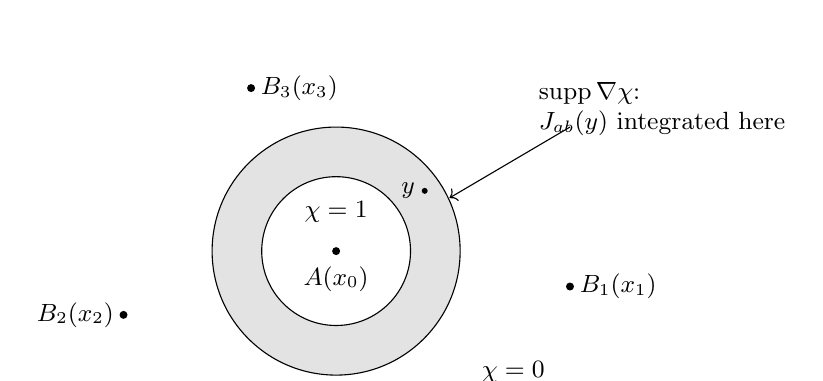
\begin{tikzpicture}[scale=0.9,font=\small]
\fill[gray!22,even odd rule] (0,0) circle (1.75) (0,0) circle (1.05);
\draw (0,0) circle (1.05); \draw (0,0) circle (1.75);
\fill (0,0) circle (1.6pt) node[below=2pt] {$A(x_0)$};
\node at (0,0.55) {$\chi=1$};
\fill (1.25,0.85) circle (1.2pt) node[left] {$y$};
\node[align=left] at (4.6,2.0) {$\operatorname{supp}\nabla\chi$:\\ $J_{ab}(y)$ integrated here};
\draw[->] (3.3,1.75) -- (1.6,0.75);
\fill (3.3,-0.5) circle (1.6pt) node[right] {$B_1(x_1)$};
\fill (-3.0,-0.9) circle (1.6pt) node[left] {$B_2(x_2)$};
\fill (-1.2,2.3) circle (1.6pt) node[right] {$B_3(x_3)$};
\node at (2.5,-1.7) {$\chi=0$};
\end{tikzpicture}
\caption{The shell flux of Definition~\ref{def:D13}. The cutoff~$\chi$ equals one near the insertion $A(x_0)$ and vanishes near the spectators $B_i(x_i)$; the current is integrated against $\nabla\chi$ on the shaded annulus. Conservation makes the flux independent of~$\chi$, so the annulus may shrink towards~$x_0$ or grow until it meets a spectator. It says nothing about flux through large spheres. The vanishing of the total angular flux at infinity is proved separately: on coordinate axes through the origin in Lemma~\ref{lem:G-collinear-flux}, and for all configurations in Lemma~\ref{lem:G3.1}.}
\label{fig:G-shell}
\end{figure}

The sign convention can be seen in one free example (Figure~\ref{fig:G-shell}). By Lemma~\ref{lem:G1.1}(iv), $\maxwellcorr_2(\curvaturesquare(x),\curvaturesquare(y))=c|x-y|^{-8}$ with $c=3\dimG/\pi^4$. The translation shell Ward identity~\eqref{eq:G-free-shells} and the free derivative law give, for a shell around~$x$,
\begin{equation*}
\mathcal P_b^{\maxwellstress}=\partial_{x_b}\bigl(c|x-y|^{-8}\bigr)=-8c\,(x_b-y_b)|x-y|^{-10}.
\end{equation*}
Replacing $\maxwellstress$ by $\lambda\maxwellstress$ multiplies this flux by~$\lambda$, so the requirement that the flux be the derivative fixes both the normalization and the sign of the stress tensor. This is a free-field calculation; nothing is asserted here about the form of interacting correlations.

The next lemmas concern only the invariant polynomial algebra of Definition~\ref{def:D11}, realized by the Taylor sections of Lemma~\ref{lem:A1}. A curvature jet of order~$j$ has weight~$j+2$. Let $\mathfrak P$ be the complex polynomial algebra on all on-shell jets, $\mathfrak P_{\le j}$ its subalgebra using orders at most~$j$, and $\mathfrak P^G$ the invariant subalgebra. The invariant polynomials of weight at most~$d$ identify with~$\maxwellspace{d}$. For a spectator degree~$d$ put
\begin{equation*}
\mathfrak N_d=\{P\in\mathfrak P:S^{\rm Max}(P(0),u_1(x_1),\ldots,u_n(x_n))=0
\text{ for all }n,\ u_i\in\maxwellspace{d},\ (0,x)\in\Conf{n+1}\},
\end{equation*}
with every polynomial Wick ordered at its own site. The degree of~$P$ is unrestricted. The next result says that spectators of one bounded degree detect every invariant polynomial, however high its jet order.
\begin{lemma}[Detection by bounded spectators]\label{lem:G-detection}
There is $d_0\in\N$ such that
\begin{equation}\label{eq:G-detection}
\mathfrak N_{d_0}\cap\mathfrak P^{G}=\{0\}.
\end{equation}
\end{lemma}
The proof has two stages. At a fixed jet order, finite generation and reflected positivity give a bound on the spectator degree. To make the bound independent of the jet order, a quadratic spectator isolates a highest-order jet derivative of~$P$ by its harmonic pole, and induction on weight removes that jet order.

The extraction rests on the difference between a single harmonic pole and a product of poles. In four dimensions $K(z)=\partial_1\partial_2|z|^{-2}=8z_1z_2|z|^{-6}$ is harmonic and homogeneous of degree $-4$; multiplication by $|z|^{4}$ leaves $8z_1z_2|z|^{-2}$, which is not analytic at zero, and only $|z|^{6}$ clears it. The product of two poles $|z|^{-2}\cdot|z|^{-2}=|z|^{-4}$ has the same degree but is already cleared by~$|z|^4$. In general a product of poles of orders $r_1,r_2\ge2$ is cleared by $|z|^{2(r_1+r_2-2)}$, while a harmonic pole of order $r_1+r_2$ needs $|z|^{2(r_1+r_2-1)}$.
\begin{proof}[Proof of Lemma~\ref{lem:G-detection}]
\emph{Step 1: bounded jet order.} Fix~$j$. The algebra~$\mathfrak P_{\le j}$ is a polynomial algebra on finitely many variables, hence Noetherian by the Hilbert basis theorem~\cite[Lemma~10.31.1]{Stacks2026}. Its ideal generated by invariant polynomials of positive ordinary degree therefore has finitely many invariant, ordinary-homogeneous generators~$f_\alpha$. Every invariant ordinary-homogeneous polynomial is a sum of products of invariant homogeneous polynomials of weight at most some~$b_j$: write $P=\sum a_\alpha f_\alpha$, keep only terms of total degree~$\deg P$, and replace $a_\alpha$ by its gauge average, whose degree is smaller; induction on the degree concludes.

Spectators of degree~$b_j$ detect: $\mathfrak N_{b_j}\cap\mathfrak P^G\cap\mathfrak P_{\le j}=\{0\}$. Otherwise take its lowest nonzero ordinary-homogeneous part~$P_r$ and split a product of homogeneous factors of total ordinary degree~$r$ into distinct nearby spectator sites. Every leg of~$P$ must pair with a spectator leg, so terms with internal spectator contractions, or with higher-degree parts of~$P$, vanish. As the spectator sites coalesce, Wick's rule gives the two-site pairing of~$P_r$ with their ordinary product. Each factor has weight at most~$b_j$, so for $P\in\mathfrak N_{b_j}$ this limit is zero. Choose the product sum to be the reflection of~$\overline{P_r}$; Lemma~\ref{lem:G1.1}(ii) makes this pairing strictly positive, a contradiction.

\emph{Step 2: pole extraction.} Put $g=\dimG$ and choose $d_0\ge\max\{b_g,2g+5\}$. In a real colour basis write $X_{j,\alpha}(p)$ for the jet coordinate tested by a scalar order-$j$ probe~$p$. For scalar probes~$p,q$ of orders $k,l$, the invariant quadratic $\sum_\alpha{:}X_{k,\alpha}(p)X_{l,\alpha}(q){:}$ has weight~$k+l+4$. Its collision with a polynomial using jets through order~$j$ has, in the coefficient where just the order-$k$ leg contracts at order~$j$, the polynomial
\begin{equation}\label{eq:G-collision}
\sum_\alpha X_{l,\alpha}(q)\sum_\mu
C_{k,j}(p,e_\mu;z)\frac{\partial P}{\partial X_{j,\alpha}(e_\mu)},
\end{equation}
where $(e_\mu)$ is a basis of order-$j$ probes and $C_{k,j}$ their differentiated curvature covariance.

\emph{Claim.} If $P\in\mathfrak N_{d_0}$, $l<k$ and $k+l+4\le d_0$, then~\eqref{eq:G-collision} lies in~$\mathfrak N_{d_0}$. Put $r=4+k+j$. Tested against fixed exterior spectators, the term~\eqref{eq:G-collision} is harmonic and homogeneous of degree~$-r$ in~$z$, so $|z|^{2(r-1)}$ times it is analytic at zero. The other terms, expanded in Taylor series at each singular order, give at order~$r$ homogeneous functions that become analytic after multiplication by $|z|^{2(r-2)}$: a double contraction is a product of poles of orders $r_1,r_2\ge2$, cleared by $|z|^{2(r_1+r_2-2)}$, and Taylor terms keep this improvement. The contraction of the order-$l$ leg alone has order at most $4+l+j<r$. The claim now follows from:
\begin{equation*}
\text{a harmonic $K$, homogeneous of degree $-r\le-2$, with $|z|^{2(r-2)}K$ analytic at $0$, vanishes.}
\end{equation*}
Indeed $\Delta(|z|^{2s}K)=4s(s+1-r)|z|^{2s-2}K$ in four dimensions; successive Laplacians show that~$K$ extends analytically, and negative homogeneity makes it zero. Expand the collision through an order exceeding $8+k+l+2j$. Since its correlation with the quadratic test and further bounded-degree spectators vanishes identically, comparing successive radial homogeneities makes the order-$r$ harmonic pole zero, so~\eqref{eq:G-collision} belongs to~$\mathfrak N_{d_0}$.

\emph{Step 3: induction on weight.} Take $k=g+1$ and $l=0,\ldots,g-1$. For each~$l$ choose a probe~$q_l$ and a jet value~$v_l$ with $q_l(v_l)=1$. The matrix $(X_{l,\alpha}(q_l))_{l,\alpha}$ has nonzero polynomial determinant: assigning~$v_l$ to colour~$l$ and zero to the other colours in order~$l$ makes it the identity. For $j>g$ the polynomial~\eqref{eq:G-collision} replaces an order-$j$ jet by an order-$l$ jet, so its weight is smaller, and the induction hypothesis makes it zero. Multiplication by the transposed cofactor matrix shows that every one-colour contraction in~\eqref{eq:G-collision} vanishes. As $z,p$ vary, the forms $C_{k,j}(p,\cdot;z)$ span the dual of the order-$j$ jets: their common annihilator generates a Maxwell wave whose order-$k$ jets vanish everywhere, a polynomial of degree below~$k$ with negative homogeneity, hence zero, and~\eqref{eq:G-kelvin} makes the probe zero. Hence every order-$j$ partial derivative of~$P$ vanishes. Descending from the top order removes all orders above~$g$; Step~1 with spectator bound~$b_g$ treats the rest.
\end{proof}

Let $\mathcal C_d$ be the real space of complex linear tuples $\mathsf X_a:\maxwellspace{d}\to\maxwellspace{d+1}$ that commute with conjugation, kill the unit, are vector-covariant under~$\hypercubic$, and send $\maxwellspace{e}$ into~$\maxwellspace{e+1}$ for $e\le d$. For $\mathsf X\in\mathcal C_d$ the Ward sum is
\begin{equation*}
\mathcal E_b(\mathsf X;\boldsymbol u,x)=\sum_i S_n^{\rm Max}(u_1,\ldots,\mathsf X_bu_i,\ldots,u_n;x).
\end{equation*}
Finitely many tests on lines determine its kernel.
\begin{lemma}[Finite vector Ward tests]\label{lem:G1-vector}
For all sufficiently large~$d$, finitely many positional derivatives of $\mathcal E_b(\mathsf X;\boldsymbol u,x)$, with $u_i\in\maxwellspace{d}$ and~$x$ on a coordinate axis through the origin perpendicular to~$e_b$, define a real linear map~$\mathcal T_d$ with
\begin{equation}\label{eq:G-free-tests}
\ker\mathcal T_d=\R\partial^{\rm Max}\quad\text{in }\mathcal C_d.
\end{equation}
\end{lemma}
\begin{proof}
Take $d\ge d_0$ from Lemma~\ref{lem:G-detection}. Suppose all the stated jets of the Ward sums of~$\mathsf X$ vanish. The free moments are translation invariant, including after a label is changed, so their Ward sums and positional jets have the same values on any parallel affine line as on the corresponding axis through zero.

\emph{Step 1: continuation off the lines.} Free correlations are real analytic off the diagonals by~\eqref{eq:G-curvature}, so every Ward sum vanishes near each testing line. For a separated configuration choose distinct ordered line coordinates respecting the strict order of its coordinates in that axis. The straight segment to the line configuration stays separated: strict inequalities persist, and coordinate ties are separated by the line coordinates. Analytic continuation along it gives $\mathcal E_b=0$ on~$\Conf{n}$.

\emph{Step 2: weight four.} Let $\mathsf J_j$ be the scalar on-shell order-$j$ jet space. For $p\in\mathsf J_0^*$ put $U(p)=\sum_\alpha{:}X_{0,\alpha}(p)^2{:}$. Simplicity, the filtration and inversion parity force $\mathsf X_bU(p)$ to be a colour contraction of one order-zero and one order-one jet, represented by a linear map $A_p:\mathsf J_0\to\mathsf J_1^*$. In the Ward identity of $U(p),U(q),U(w)$ let the first two points coalesce along~$tu$ and multiply by~$t^5$. The term with $\mathsf X_b$ at the distant point tends to zero, and the two remaining triangular Wick contractions give, for every $X\in\mathsf J_0$ and with $C_{1,0}$ taken in one colour,
\begin{equation*}
C_{1,0}(A_pX,q;u)\,q(X)=C_{1,0}(A_qX,p;u)\,p(X).
\end{equation*}
Arbitrary~$X$ are reached by choosing the distant probe~$w$ through the invertible order-zero covariance~\eqref{eq:G-kelvin}. If $p(X)=0$, choose $q(X)\ne0$; varying $q,u$ gives $A_pX=0$. Thus $A_pX=p(X)f_bp$, and the same identity shows that $f_b:\mathsf J_0^*\to\mathsf J_1^*$ is real linear with $C_{1,0}(f_bp,q;u)=C_{1,0}(f_bq,p;u)$.

\emph{Calculation of~$f_b$.} Write $e^{ij}$ for the curvature coordinate and $\partial_he^{ij}$ for its first jet. For $f_1e^{12}$, sign parity permits only $\partial_1e^{12},\partial_3e^{23},\partial_4e^{24}$; interchange of axes~$3,4$ and $\sum_i\partial_ie^{i2}=0$ reduce their span to $\R\partial_1e^{12}$. For $f_1e^{23}$ the candidates $\partial_1e^{23},\partial_2e^{13},\partial_3e^{12}$ reduce, by antisymmetry in axes~$2,3$ and Bianchi, to $\R\partial_1e^{23}$. Permutations leave two constants, which agree because $C_{1,0}(\partial_1e^{12},e^{23};e_1+e_3)=-1/(2\pi^2)\ne0$ by~\eqref{eq:G-curvature}. Therefore $f_b=c_{\rm jet}\partial_b$, and since $\partial_bU(p)$ has two identical terms, $\mathsf X_b=c\,\partial^{\rm Max}_b$ on weight four with $c=c_{\rm jet}/2$.

\emph{Step 3: higher weights.} Set $\mathsf X^\circ_b=\mathsf X_b-c\,\partial^{\rm Max}_b$. Translation invariance makes its Ward sums zero, and it kills every free stress component. Insert into such a sum a free stress shell for the dilation field $v(y)=y-x_0$, surrounding only the distinguished point. The term where $\mathsf X^\circ_b$ acts on the stress is zero. The other shell terms are given by the polarized calculation in Lemma~\ref{lem:G1.1}, now with this~$v$; the extra derivative of~$v$ contracts with the trace of the free stress, which is zero by~\eqref{eq:G-free-tensor}. The local Lie derivative of a two-form under dilation is $y\cdot\nabla+2$, and on jets it gives the weight operator $\mathsf D^{\rm wt}X_{j,\alpha}=(j+2)X_{j,\alpha}$. Subtracting the Ward sum with distinguished label~$\mathsf D^{\rm wt}u$ shows $[\mathsf D^{\rm wt},\mathsf X^\circ_b]u\in\mathfrak N_d$, and Lemma~\ref{lem:G-detection} makes it zero. So $\mathsf X^\circ_b$ preserves each weight. Inversion acts there by~$(-1)^{\rm weight}$, whereas vector covariance makes $\mathsf X^\circ_b$ odd under inversion; hence $\mathsf X^\circ_b=0$.

\emph{Step 4: finite selection.} Conversely translation invariance annihilates every test on~$\partial^{\rm Max}$. The real space~$\mathcal C_d$ is finite-dimensional; successively choose a test nonzero on the current kernel modulo this line. Each choice lowers its dimension, so finitely many tests have precisely the asserted kernel.
\end{proof}

The internal tests rest on one elementary fact about the plane generators $K_{ab}=E_{ba}-E_{ab}$ of $\mathfrak{so}(4)$. Call a coordinate quarter turn the rotation $e_a\mapsto e_b$, $e_b\mapsto-e_a$ in one coordinate plane.
\begin{lemma}[Alternating planes]\label{lem:G-planes}
Let $\beta:\mathfrak{so}(4)\times\mathfrak{so}(4)\to V$ be real bilinear and alternating, with $\beta(hKh^{-1},hLh^{-1})=\beta(K,L)$ for every coordinate quarter turn~$h$. Then $\beta=0$.
\end{lemma}
\begin{proof}
The quarter turns generate the determinant-one signed permutations: they project onto the transpositions of $S_4$, and squares of quarter turns give the diagonal sign changes with two minus signs. Conjugation by a diagonal sign matrix~$s$ multiplies $K_{ab}$ by $s_as_b$; conjugation by a permutation matrix permutes the planes. \emph{Overlapping planes:} $s=\operatorname{diag}(1,1,-1,-1)$ fixes $K_{12}$ and reverses the sign of $K_{13}$, so $\beta(K_{12},K_{13})=-\beta(K_{12},K_{13})=0$. \emph{Disjoint planes:} the even permutation $(13)(24)$ interchanges $K_{12}$ and $K_{34}$, so $\beta(K_{12},K_{34})=\beta(K_{34},K_{12})=-\beta(K_{12},K_{34})=0$. Every pair of distinct planes is carried to one of these two pairs by a signed permutation of determinant one, and $\beta(K,K)=0$; bilinearity gives $\beta=0$.
\end{proof}

Let $\mathcal B_d$ consist of alternating real-bilinear families $\Delta:\mathfrak{so}(4)^2\to\operatorname{End}_{\C}\maxwellspace{d}$ which commute with conjugation, kill the unit, preserve every lower-degree subspace, and satisfy
\begin{equation*}
R^{\rm Max}(h)\Delta(K,L)=\Delta(hKh^{-1},hLh^{-1})R^{\rm Max}(h)
\qquad(h\in\hypercubic,\ \det h=1).
\end{equation*}
The next result removes the defect in the rotation commutator.
\begin{lemma}[Finite internal Ward tests]\label{lem:G1-internal}
For every $d\ge4$, finitely many sums
\begin{equation}\label{eq:G-erasure-test}
\sum_i S_n^{\rm Max}(u_1,\ldots,\Delta(K,L)u_i,\ldots,u_n;x),
\qquad u_i\in\maxwellspace{d},\quad x\in\Conf{n},
\end{equation}
separate~$\mathcal B_d$.
\end{lemma}
\begin{proof}
Suppose all these sums vanish and fix $\mathsf Z=\Delta(K,L)$. The arity-one Ward condition gives $S_1^{\rm Max}(\mathsf Zu)=0$. Since $\mathsf Z$ preserves degree and kills the unit, this excludes a unit component in the image of a centered weight-four field; the centered weight-four space is invariant. On that space let $b_x(u,v)=S_2^{\rm Max}(u,v;x,0)$. The order-zero Kelvin formula and Wick's rule give $b_x(u,v)=b_y(R^{\rm Max}(\mathcal R_y\mathcal R_x)u,v)$ for $|x|=|y|\ne0$. Both $\mathsf Z$ and the orthogonal action preserve this space. Applying $b_x(\mathsf Zu,v)+b_x(u,\mathsf Zv)=0$ at~$x$ and~$y$, and nondegeneracy of~$b_y$, shows that~$\mathsf Z$ commutes with $R^{\rm Max}(\mathcal R_y\mathcal R_x)$, in particular with every coordinate quarter turn. With the signed covariance of~$\Delta$, the function $(K,L)\mapsto\Delta(K,L)u$ satisfies the hypothesis of Lemma~\ref{lem:G-planes} for each weight-four~$u$, so~$\mathsf Z$ vanishes on weight four, including the stress.

Insert a free angular stress shell around the distinguished point only, as in Step~3 of the proof of Lemma~\ref{lem:G1-vector}. Subtracting the Ward sum with the angularly differentiated label gives $[\mathsf L^{\rm Max}(M),\mathsf Z]u\in\mathfrak N_d$. This polynomial has weight at most~$d$, so Lemma~\ref{lem:G1.1}(ii) makes it zero. Hence $\mathsf Z$ commutes with all infinitesimal rotations, and differentiating $e^{t\mathsf L(M)}\mathsf Z-\mathsf Ze^{t\mathsf L(M)}$ gives commutation with coordinate quarter turns in every degree. Lemma~\ref{lem:G-planes} again gives $\Delta=0$. Finite-dimensionality selects a finite separating subfamily by successively reducing the common kernel.
\end{proof}

\subsection{Lattice inputs}\label{sec:G-lattice}

The insertions are those of Definition~\ref{def:D08}, with coefficient polynomials from Definition~\ref{def:D19} and Lemma~\ref{lem:A1}. The inverse coefficient estimate of Lemma~\ref{lem:E-marked-step} inverts the marked coefficient map; the corrected sources and normalized integral of Lemmas~\ref{lem:E-Gaussian-sources} and~\ref{lem:E-source-integral} bound the remainders; the uniform displacement estimate of Lemma~\ref{lem:E-displacement} controls positions, with coordinate separations at least four times the displacement margin. Chessboard seminorms are those of Definition~\ref{def:D27}. Cutoff limits are taken in the order~\eqref{eq:E2-tails}, followed by the fixed extraction of Lemma~\ref{lem:F1}; an ordered limit point of a bounded coefficient family is its limit along an ultrafilter containing the ordered tails.

Fix arity and degree bounds $n\ge2,D\ge1$ and $R\ge1$. A basis word is a list of members of fixed real bases of $\maxwellspace{d}$, $d\le D$. Put
\begin{equation*}
K_{R,m}=\{x:|x|\le R,\ \sepinf(x)\ge R^{-1}\},\qquad
E_\delta=\{x:|x_i^a-x_j^a|>\delta\ (i\ne j,\ a=1,\ldots,4)\}.
\end{equation*}
The comparison exponents $\alpha_0,\alpha_1,\alpha_2>0$ and $c<0$ have the following roles: $\alpha_0$ sets the comparison radius, $\alpha_1$ the cells used for moment bounds, $\alpha_2$ the smaller cells used for displacement bounds, and~$c$ the width of the excluded coordinate strips. They satisfy
\begin{equation}\label{eq:G-exponents}
\alpha_1+6<\alpha_0,\quad \alpha_2+5<\alpha_0+c,\quad
(\alpha_0-\alpha_1)Dn+c<0,\quad
(\alpha_0-\alpha_2)Dn-\alpha_0-c<0.
\end{equation}
The first two inequalities place the chessboard cells; the last two make the excluded strips negligible. One explicit choice, with $n_{\max}=\max(n,D)$, is $\kappa_1=7n_{\max}(n_{\max}+2)+1$, $\kappa_2=6+\kappa_1$, $\alpha_0=17+n_{\max}+\kappa_1+\kappa_2n_{\max}(n_{\max}+2)+\kappa_2$, $\alpha_1=\alpha_0-7$, $\alpha_2=\alpha_0-\kappa_2$ and $c=-\kappa_1$. Write $M_k=\cutoffsize_k$ and set
\begin{equation}\label{eq:G-balance}
r_k=a_kM_k^{\alpha_0},\qquad \mathfrak s_k=M_k^{-\alpha_0},\qquad
\delta_k=M_k^{c},\qquad
R^{\rm cell}_k=CM_k^{(\alpha_0-\alpha_1)D},\quad R^{\rm var}_k=CM_k^{(\alpha_0-\alpha_2)D},
\end{equation}
where $C\ge1$ depends only on $n,D,R$ and the construction and is fixed in the proof of Lemma~\ref{lem:G-lattice}. Thus $r_k\mathfrak s_k=a_k$: the normalized grid is the physical construction grid. For an ordered limit point $c_{k,d}:\maxwellspace{d}\to V_d$ of the lifts in Lemma~\ref{lem:G-lattice}, and the quotient $\pi_d:V_d\to F_d$ of Definition~\ref{def:D10}, define the rescaled correlation
\begin{equation*}
S^{\rm sc}_k(\boldsymbol u;x)=S_m(\pi_{d_i}c_{k,d_i}u_i;r_kx).
\end{equation*}

The following comparison uses one coefficient family for every word within the fixed bounds. Its constants may depend on these bounds, the word and the construction. The arity, degree and radius bounds are fixed first, then the level and the lifts; the estimates then hold for every basis word within these bounds.
\begin{lemma}[Lattice comparison at small radii]\label{lem:G-lattice}
There are arbitrarily large levels~$k$, real $\hypercubic$-equivariant lifts $\Lambda_{k,N,p,d}:\maxwellspace{d}\to V_d$ preserving the degree-zero unit, and $\varepsilon_k\to0$ such that every ordered limit point of these lifts satisfies, for every basis word with $m\le n$,
\begin{equation}\label{eq:G-lattice-input}
\begin{aligned}
|S^{\rm sc}_k|&\le (R^{\rm cell}_k)^m &&\text{on }K_{R,m},\\
\|\nabla S^{\rm sc}_k\|&\le4m (R^{\rm var}_k)^m/\delta_k &&\text{on }K_{2R,m}\cap E_{4\delta_k},\\
|S^{\rm sc}_k-S_m^{\rm Max}|&\le\varepsilon_k
&&\text{on }(\mathfrak s_k\Z)^{4m}\cap K_{2R,m}\cap E_0.
\end{aligned}
\end{equation}
At fixed~$k$ the lifts are bounded on ordered tails.
\end{lemma}
The lifts are chosen so that the rescaled insertions have the free Wick polynomials as Gaussian leading part~\eqref{eq:G-lift-equation}. A subset recursion removes the continuum Gaussian moments; for exact Gaussian variables each remainder has mean zero, and the source estimates of Section~\ref{sec:partII-E} make each remainder small in chessboard seminorm~\eqref{eq:G-source-root}. The chessboard inequality then gives the comparison on the grid, and the coarser normalizations $\alpha_1,\alpha_2$ give the size and gradient bounds off the grid.
\begin{proof}
\emph{Step 1: lifts.} Choose a real $\hypercubic$-equivariant polynomial representative map $\iota_d^{\rm free}$ for the on-shell quotient, using the Taylor sections of Lemma~\ref{lem:A1} and averaging a real splitting over~$\hypercubic$. For a reference label $c\in V_d$ let $\mathsf M_{k,N,p,d}c=\mathbf x_k(\mathsf Z_{N,p,d}^{-1}c)$ be its actual level-$k$ marked coordinate, and put $\mathsf A_{k,N,p,d}=a_k^{-d}\mathsf M_{k,N,p,d}$. Thus $\mathsf A$ maps reference labels to spacing-normalized level-$k$ coefficients; the physical primary additionally applies $t_k^{-\factorcount}$. In particular $\mathsf A\mathbf u_d=\mathbf1$. Let $\mathsf C_{k,N,p,d}:V_d\to V_d$ be the tested coefficient map from the reference copy to the level-$k$ tested-coefficient copy, in these same spacing-normalized, threshold-weighted coordinates. The lift construction requires $\mathsf C\mathbf u_d=\mathbf1$, conjugation and signed-permutation covariance, and the Gaussian leading-polynomial and Wick-ordering identification of Lemma~\ref{lem:E-source-polynomial}. It also requires $|(\mathsf C-\mathsf A)c|_1\le\eta_k|\mathsf A c|_1$ for every~$c$, uniformly on the relevant cutoff tails, with $\eta_k\le\tfrac14$. These tested-map identifications and the relative estimate are conditional on the actual common-sample coefficient comparison; invertibility of an unspecified Wick change alone does not give them. Write $\delta_t^{\rm wt}$ for multiplication of a weight-$j$ monomial by~$t^j$; the factor-count scaling~$t^{\factorcount}$ is that of Definition~\ref{def:D08}. The Gaussian field divided by the small-field threshold has scale
\begin{equation*}
\mathfrak t_{k,N,p}=(t_k\sqrt{\beta_{N,p,k}})^{-1},\qquad
0<\mathfrak t_{k,N,p}^{-1}\le2M_k,
\end{equation*}
since $t_k=M_k/\sqrt{\refbeta_k}$ is the small-field threshold of Part~I and $\beta_{N,p,k}\le2\refbeta_k$. Solve
\begin{equation}\label{eq:G-lift-equation}
\mathsf C_{k,N,p,d}\Lambda_{k,N,p,d}u
=\mathfrak t_{k,N,p}^{-\factorcount}\delta_{M_k^{\alpha_0}}^{\rm wt}\iota_d^{\rm free}u.
\end{equation}
The solution exists and obeys
\begin{equation}\label{eq:G-lift-bound}
|v|_1\le K_{k,d}a_k^d|\mathsf C_{k,N,p,d}v|_1,
\end{equation}
with $K_{k,d}$ independent of~$N,p$ at fixed~$k$. Indeed, $\mathsf M^{-1}$ carries a level-$k$ coordinate down to the reference level. Applying Lemma~\ref{lem:E-marked-step} along those finitely many steps gives $|c|_1\le K'_{k,d}a_k^d|\mathsf A c|_1$ for a product $K'_{k,d}$ of column and block factors. The stated relative estimate gives $|\mathsf A c|_1\le(1-\eta_k)^{-1}|\mathsf C c|_1\le2|\mathsf C c|_1$, proving~\eqref{eq:G-lift-bound} with $K_{k,d}=2K'_{k,d}$. It also makes $\mathsf C$ injective, hence invertible in finite dimension. Its unit, conjugation and signed laws pass to the inverse. The bound on~$\mathfrak t^{-1}$ bounds the right side at fixed~$k$, so the lifts are bounded on cutoff tails, conditional on the tested-map inputs.

\emph{Step 2: subset recursion.} This step uses the actual common-sample guarded reading and forecast comparison, together with charged regular, forced and scalar source estimates, in Lemma~\ref{lem:E-source-polynomial}. If a restarted comparison is used, its density and couplings below the restart must be those of the same comparison course. The finite Gaussian subset algebra alone does not supply this input; without it the grid comparison~\eqref{eq:G-lattice-input} remains conditional. Under those inputs, apply Lemmas~\ref{lem:E-source-polynomial}--\ref{lem:E-source-integral} for an arity bound~$n\ge2$, at most~$n$ marks per cell and any compact position set with positive point separation, on the interval~\eqref{eq:E-window} with exponent~$\alpha_0$ and position set~$K_{2R,m}$. Their covariance and Taylor bounds are uniform on $K_{2R,m}$, whose point separations are at least $(2R)^{-1}$, and need no lower bound on coordinate differences; only the reflected placement below requires~$E_0$. Write $I_i=O_{N,p}^{(d_i)}(\Lambda_{k,N,p,d_i}u_i,r_kx_i/a_N)$ at compatible lattice points. For a subset~$J$ put $G_J=S_{|J|}^{\rm Max}((u_i)_{i\in J};(x_i)_{i\in J})$ and define
\begin{equation*}
R_\varnothing=1,\qquad
R_I=\prod_{i\in I}I_i-\sum_{\varnothing\ne J\subseteq I}G_JR_{I\setminus J}.
\end{equation*}
This subtracts the full continuum Gaussian moment on every subset of slots; for exact continuum Gaussian variables its nonempty coefficients have expectation zero, by induction on~$|I|$. The Wick-ordering correction and~\eqref{eq:G-lift-equation} identify the leading Gaussian correlations with these continuum moments at the normalized grid points, as calculated in Lemma~\ref{lem:E-source-polynomial}. Covariance, Taylor and localization errors remain in the regular and forced source terms.

\emph{Step 3: chessboard seminorm of the remainders.} The replicated-source and stopping estimate used here additionally requires the support-weighted containing-site envelope of Lemma~\ref{lem:E-source-attachments} for actual mixed-degree higher modes, including inherited higher factors and new singleton joins, together with its exponent-98 stopping restart. It also requires the complete initial shared-forced modes and the coefficient majorant divided by the original positive density. Singleton bounds by themselves do not give these inputs. Until these inputs are established, the root estimate~\eqref{eq:G-source-root}, and consequently the comparison in Lemma~\ref{lem:G-lattice}, are conditional on it. The finite-set clause of Lemma~\ref{lem:E1.1} gives arbitrarily late common terminal levels~$k$ for the three exponents $\alpha_0,\alpha_1,\alpha_2$. Use the interval~\eqref{eq:E-window} with exponent~$\alpha_0$, its width level $w_{\alpha_0}(k)=k-h_k(\alpha_0)-v_k$ and its centered tiling $\mathcal C^{\rm tile}_{w_{\alpha_0}(k)}(0)$. Put $q_k=\log M_k/(16n)$ and give each mark weight $e^{2q_k}\le M_k^{1/16}$. The weighted mode norm in the proof of Lemma~\ref{lem:E-replication} multiplies mark weights over subsets, so coefficient extraction for a nonempty~$I$ contributes $e^{-2q_k|I|}$ in each reflected cell, and the corrected-source iteration of Lemma~\ref{lem:E-Gaussian-sources} keeps this mark weight on the selected comparison intervals. Work in $\C[z_1,\ldots,z_m]/(z_i^2)$ and multiply by the reciprocal of the continuum free moment polynomial; its coefficient of~$z_I$ is exactly~$R_I$. After the finite Gaussian contractions on every subset, the remaining source modes have zero leading Gaussian coefficient. In the source iteration, terms linear in these modes cost the finite stage constant, and every other connected term contains at least two residual modes and is bounded by their squared norm times a fixed power of~$M_k$; this is~\eqref{eq:E-source-step}. The covariance and localization errors of Lemma~\ref{lem:E-source-polynomial} are below the corresponding source tolerance at entry~\eqref{eq:E-source-iteration}. Lemma~\ref{lem:E-Gaussian-sources}, applied to the coefficients~\eqref{eq:E-corrected-coefficients} of these finitely many subset modes, gives this mark weight with constants depending only on $n,D,R$ and the construction; its sums are rooted at a mark and do not count the replicated cells.

The normalized positive integral costs, per cell, at most the stage constant $Q_{J_k}^{\rm cmp}$ of~\eqref{eq:E-comparison-cost} (Lemma~\ref{lem:E-source-integral}), which includes $2+2n$ for the scalar, unmarked forced gas, and regular and forced source sums for at most~$n$ marks. Item~\ref{it:E-entries} imposes $Q_j^{\rm cmp}\le\log M_t/(16n)$ for each arity bound, hence $Q_{J_k}^{\rm cmp}\le q_k$; the entry is chosen after the finitely many source constants. Taking the root over the reflected cells gives
\begin{equation}\label{eq:G-source-root}
\|R_I\|_{\mathcal C^{\rm tile}_{w_{\alpha_0}(k)}(0)}
\le e^{q_k-2q_k|I|}\le M_k^{-1/(16n)}
\qquad(\varnothing\ne I\subseteq\{1,\ldots,m\}).
\end{equation}
The smallness comes from the corrected density at large coupling: its source terms stay bounded at a growing mark weight, while the unmarked normalization grows more slowly than that weight. The estimate concerns the complete reflected array, before absolute values are taken, and needs no independence of the insertions.

\emph{Step 4: comparison on the grid.} Distinct coordinate differences at normalized grid points are at least $\mathfrak s_k$, so their physical differences are at least~$a_k$. The reading map assigns the corresponding level-$k$ sites without rounding, and the interval margin~\eqref{eq:E-window-geometry} contains the inspected stencils and their reflected copies. Expanding the recursion, applying~\eqref{eq:E-chess} to each~$R_I$ and bounding the free submoments on~$K_{2R,m}$ gives $C_{R,\boldsymbol u}M_k^{-1/(16n)}$, the last line of~\eqref{eq:G-lattice-input}.

\emph{Step 5: size and variation off the grid.} At its own normalization the singleton comparison gives a chessboard seminorm at most $1+|S_1^{\rm Max}(u)|$. For exponent~$\alpha_1$, changing normalization to~$M_k^{\alpha_0}$ multiplies a weight-$j$ coefficient by $M_k^{(\alpha_0-\alpha_1)j}$, so the finite coefficient sum bounds these seminorms by~$R^{\rm cell}_k$ for~$C$ large; exponent~$\alpha_2$ gives~$R^{\rm var}_k$. Include every reflected basis label and its complex conjugation in these maxima. The two interval lengths of~\eqref{eq:E-window} give, with the stage block ratio~$L$,
\begin{equation}\label{eq:G-root-sides}
\frac{a_{w_b(k)}}{a_k}=L^{h_k(b)+v_k}
\le L^2M_k^{b+2}B_k^{10}\le M_k^{b+5}
\qquad(b=\alpha_1,\alpha_2),
\end{equation}
after the stage entry, where $L$ is fixed and $B_k=M_k^{o(1)}$. So the $\alpha_1$ cell is at most $a_kM_k^{\alpha_1+6}=o(r_k)$ and the $\alpha_2$ cell is $o(r_k\delta_k)$ by~\eqref{eq:G-exponents}. The chessboard inequality bounds separated continuum moments by~$(R^{\rm cell}_k)^m$. The physical diameter on~$r_kK_{2R,m}$ is at most $4Rr_k<L_p/2$ on the ordered tails, so the torus separation~$g_p$ of Lemma~\ref{lem:E-displacement} is the minimum ordinary coordinate separation, which exceeds $4r_k\delta_k$ on~$E_{4\delta_k}$. The uniform clause of Lemma~\ref{lem:E-displacement}, with margin $r_k\delta_k$ and the reflected seminorms included in~$R^{\rm var}_k$, gives $4m(R^{\rm var}_k)^m/\delta_k$ after rescaling. The three normalizations use the same coefficient map and lifts and the same terminal levels; the finitely many cutoff tails can be intersected.

\emph{Step 6: limits.} The passage to the fixed-period table uses the selected one-mark convergence of Lemma~\ref{lem:E-fixed-level}. Its common-core argument requires actual finite trajectories and contracting steps on a common complete graph class with the original address and eligibility tests, convergence on a dense finite-address core in the full regular derivative and forced norms with output tails, and a uniform same-cutoff Lipschitz bound for the coefficient readout. It is conditional on these inputs; convergence of unmarked coordinates alone does not give it. Take any ordered limit point of the bounded lifts. Lemma~\ref{lem:E3.1} and~\eqref{eq:F-conf} pass the moment estimates to the fixed table, and Proposition~\ref{prop:FC} with Lemma~\ref{lem:F2} passes the difference bound. No extraction of the table or the volume sequence is made.
\end{proof}

For the shell estimate take $\varkappa\in\{0,1\}$, $A\in F_d$, $B\in F_4$ and $D=d+1-\varkappa$. The shell factor has scaling degree $3+\varkappa$: integration over four dimensions contributes four powers of the radius, the differentiated cutoff removes one, and the constant or linear vector field contributes~$\varkappa$. Since the two inserted fields have total degree $d+4$, the expected output degree is $(d+4)-(3+\varkappa)=D$. A grid test is a separated configuration $(0,x_i)$ on $a_{j_0}\Z^4$ for some level~$j_0$, generic in each coordinate, with a fixed spectator list~$\boldsymbol B_i$. Its response functional and marked response are
\begin{equation*}
\mathsf r_i(v)=S(v(0),\boldsymbol B_i(x_i)),\qquad
\mathfrak h_i(y)=S(B(y),A(0),\boldsymbol B_i(x_i)).
\end{equation*}
For example, for a translation shell in direction~$1$, take $A=\scaleframe{k}{4}\curvaturesquare\in F_4$ and $B=J_{11}\in F_4$, where $J$ is the conserved tensor of Lemma~\ref{lem:G2.2}. Here $D=5$, and $\mathsf r_i:F_5\to\C$ tests a degree-five field against the same fixed spectators as $\mathfrak h_i(y)=S(J_{11}(y),A(0),\boldsymbol B_i(x_i))$. Finite collections may use different grids, and the union of all these configurations is dense. The next lemma shows that every finite combination of tests annihilating $F_D$ also annihilates the limiting shell response.
\begin{lemma}[Annular annihilator estimate]\label{lem:G-annular}
For every finite list of grid tests and coefficients $g_i\in\C$ with $\sum_i g_i\mathsf r_i=0$ on~$F_D$, there are $\rho_l\downarrow0$ such that
\begin{equation}\label{eq:G-annular-input}
\sup_{1/4\le|z|\le2}\left|\sum_i g_i\rho_l^{3+\varkappa}\mathfrak h_i(\rho_lz)\right|\longrightarrow0.
\end{equation}
\end{lemma}
\begin{proof}
The local sections of Lemma~\ref{lem:A1} and Lemmas~\ref{lem:E2.2}--\ref{lem:E2.3} represent the product of two nearby marked insertions by one marked insertion of degree~$D$; Proposition~\ref{prop:FC} and Lemma~\ref{lem:F2} pass to the quotient. Put $h=3+\varkappa$, so $D+h=d+4$. Recall $s_m=\log(a_m^{-1})$ from~\eqref{eq:I12-levels}. Use the support radius $B_m=\lceil(\log\refbeta_m)^2\rceil$ of Part~I and take $\rho_m=128B_{m+1}^2a_{m+1}$, so $\log\rho_m=-s_m+o(s_m)$.

\emph{Step 1: two-mark representation.} Passing the two-mark grid tests to the fixed table uses the selected one-mark convergence of Lemma~\ref{lem:E-fixed-level}, conditional on its common-core, finite-trajectory, output-tail and coefficient-readout inputs. The lemma does not itself establish the mixed and higher-mode estimates: these must apply to the actual finite-cutoff construction on its original addresses, with both anchors, eligibility tests and the needed tails. Step~3 uses convergence of the tested moments to the fixed table, a bounded coefficient limit point and a uniform finite-cutoff residual bound; it does not require convergence of the merged graph itself. Convergence of unmarked coordinates alone is insufficient. Thus the ordered mixed-table limit used in Step~3 is conditional on these fixed-period inputs. The present two-mark calculation also requires the complete initial mixed-degree source for grades $d$ and $4$, including every eligible shared-forced term, and the grade-$D$ coefficient inverse. The fixed-stopping backward and residual estimates must apply to the merged regular/forced remainder with both original anchors and the degree-$D$ subtraction at zero. These are separate inputs from the Gaussian comparison and its normalized integral in Lemma~\ref{lem:G-lattice}. Fix a centered cell around the distinguished point, disjoint from all spectator stencils, and a finer stopping level~$k_0\ge\reflevel{D}$ at which its replicated source estimate applies. Choose levels~$j(m)$ with
\begin{equation*}
\frac{s_{j(m)}}{s_m}\longrightarrow t=1+\frac1{64(d+12)};
\end{equation*}
they exist since $s_{m+1}/s_m\to1$ (Lemma~\ref{lem:E1.1}). At a grid point $y\in a_{j(m)}\Z^4$ with $\rho_m/16<|y|<4\rho_m$, choose representatives $a\in V_d,b\in V_4$ of~$A,B$, block their two marked insertions at~$y,0$ together, and retain the Taylor terms of weight at most~$D$. Treat the physical product, including the factor $\rho_m^h$, as one degree-$D$ mark. At level~$j$ use the $a_j^{-D}t_j^{-\factorcount}$ convention of Definition~\ref{def:D08} and the marked step factor $\ell_j^D$ in~\eqref{eq:I12-marked-evolution}. Carry its complete source to the reference level $\reflevel{D}$ and let $q_{N,p}(y)$ be its degree-$D$ marked coordinate in that same normalization. Choose $c_{N,p}(y)=q_{N,p}(y)$, so that the degree-$D$ coordinate of the difference vanishes at that level. The required uniform bound on $q_{N,p}(y)$ for each fixed~$m,y$ is part of the actual mixed-source transport input, including the original eligibility tests and support tails. The exact difference is
\begin{equation*}
\rho_m^h O_{N,p}^{(4)}(b,y/a_N)O_{N,p}^{(d)}(a,0)
 -O_{N,p}^{(D)}(c_{N,p}(y),0).
\end{equation*}
Let $u_{m,1},u_{m,2}$ be the available mark weights of the degree-$d$ and rescaled degree-four marks at level~$j(m)$. The one-mark bounds, including~$\rho_m^h$, give $\log u_{m,1}=(-dt+o(1))s_m$ and $\log u_{m,2}=(-4t+h+o(1))s_m$; support weights, coefficient columns and threshold powers have logarithm~$o(s_m)$ by~\eqref{eq:E-marker-scales} and~\eqref{eq:E-log-cost}. Transporting each source to level~$m+1$ adds the volume factor $(a_{j(m)}/a_{m+1})^4$ to its weight. The two-mark input must bound the complete starting data at level~$m+1$: its degree-$D$ normalized jet $q_{m+1}$ and the merged regular and normalized forced remainder of norm $r_{m+1}$. Denote a bound for $|q_{m+1}|_1+r_{m+1}$ by~$e_m$, uniform in $N,p$ and the permitted grid points. The required joint weight~$v_m$ and starting bound satisfy
\begin{equation}\label{eq:G-annular-cost}
\log v_m=[-D-(d+12)(t-1)+o(1)]s_m,\qquad
e_m\le\exp\{[(d+12)(t-1)+o(1)]s_m\}.
\end{equation}
Indeed the transported exponents sum to $-(d+4)t+h+8(1-t)=-D-(d+12)(t-1)$, and Taylor extraction costs the reciprocal joint weight times~$a_{m+1}^D$, which cancels the~$D$ term. Applying this price to the complete starting data is an additional mixed-source estimate, including the selected insertion and every forced term with its eligibility test; a bound on the Taylor remainder alone does not supply it.

\emph{Step 2: backward matching.} Let $C_m=C^{\rm col}_{J_{m+1}}$ and let $T$ be the top remainder norm after the selected insertion has been subtracted. The matching cone gives $|\Delta_{m+1}|_1\le T/[32(1+C_m)^2]$; the selected insertion bound then gives $T\le r_{m+1}+C_m(|q_{m+1}|_1+|\Delta_{m+1}|_1)\le2(r_{m+1}+C_m|q_{m+1}|_1)$. The constant and column cost have logarithm $o(s_m)$, so they are absorbed into~$e_m$. This application is conditional on the mixed-source norm and cone for the same subtraction. Apply~\eqref{eq:E-backward-match-level} from~$m+1$ to the fixed stopping level~$k_0$. The matched remainder gains $\prod_{i=k_0}^{m}\ell_i^{1/8}=e^{(s_{m+1}-s_{k_0})/8}\ge e^{(s_m-s_{k_0})/8}$ in its inverse bound. Put $c_m=e^{s_m/32}$ and multiply the source by~$c_m$; its size is then at most
\begin{equation*}
c_me_me^{-(s_m-s_{k_0})/8}
\le\exp\{[-5/64+o(1)]s_m\},\qquad
\tfrac1{32}+(d+12)(t-1)-\tfrac18=-\tfrac5{64},
\end{equation*}
which tends to zero and therefore falls below any fixed positive tolerance at~$k_0$. In particular, the required controlled-source criterion has weighted singleton exponential bound at most~$3$, forced singleton bound at most~$1$, and connected regular and forced bounds at most one each per mark, with the original eligibility tests and intervening attachment bounds as specified before Lemma~\ref{lem:E-replication}; its application to this merged source remains conditional on the input in Step~1. The residual-source estimate~\eqref{eq:E-residual-root} at the fixed cell and level~$k_0$ then bounds the chessboard seminorm of the unamplified residual by~$2C/c_m$, with~$C$ independent of~$m,N,p$. The reference-level matching coordinate $c_{N,p}(y)=q_{N,p}(y)$ is bounded on cutoff tails for each fixed~$m,y$ under the mixed-source transport input of Step~1. This match uses the actual marked construction, independently of the tested map~$\mathsf C$. Interior support follows from $32\rho_m\to0$ and the support diameter $a_{m+1}(B_{m+1}^2+1+2048B_{m+1}^2)\to0$.

\emph{Step 3: cancellation at grid points.} Pass to an ordered limit point~$c(y)$ and project it to~$F_D$. The chessboard inequality~\eqref{eq:E-chess} for the residual and the fixed exterior stencils gives, simultaneously for the finite tests,
\begin{equation*}
|\rho_m^h\mathfrak h_i(y)-\mathsf r_i(\pi_Dc(y))|\le C_i c_m^{-1},
\end{equation*}
with the same coefficient vector for every spectator. Multiplication by~$g_i$ and summation cancel the response term, so $f_m(y)=\sum_i g_i\rho_m^h\mathfrak h_i(y)$ is $O(c_m^{-1})$ at all grid points of the enlarged annulus whose four coordinates are nonzero.

\emph{Step 4: interpolation across coordinate planes.} For a derivative order~$q$, Proposition~\ref{prop:FC} replaces the moving label by one of degree $4+q$. The centered and reflected bounds of Lemmas~\ref{lem:E2.3} and~\ref{lem:E-replication}, with~\eqref{eq:E-chess}, bound a field of fixed degree~$e$ by $\exp[(e+2+o(1))s_m]$, with a field-dependent constant of logarithm~$o(s_m)$. The finitely many later levels required for the fixed spectator word have logarithmic scale $s_m+o(s_m)$. Choose degree bounds~$e_{ij}$ for the spectator labels and put $C_0=8+d+\max_i\sum_j(e_{ij}+2)$. Since $\rho_m^h\le1$,
\begin{equation}\label{eq:G-annular-derivatives}
|\partial_a^q f_m(y)|\le \exp[(q+C_0+o(1))s_m]
\qquad(\rho_m/16<|y|<4\rho_m),
\end{equation}
with $C_0$ independent of~$q$. Choose $q$ with $q(t-1)>C_0$; since $a_{j(m)}=\exp[-(t+o(1))s_m]$, the scaled remainder $a_{j(m)}^q\sup|\partial_a^q f_m|$ on grid-sized segments tends to zero. At each interpolation stage the previously treated coordinates may be arbitrary, and the remaining untreated coordinates are nonzero lattice grid points. On the moving coordinate segment of length $4(2^q+2)a_{j(m)}$, choose $q$ nonzero grid nodes separated by at least $a_{j(m)}$, keeping all other coordinates fixed. Lagrange interpolation gives $|g|\le C_q(\max_{\rm nodes}|g|+a_{j(m)}^q\sup|\partial^qg|)$ on the segment, with $C_q$ independent of~$m$. Apply it to ${\rm Re}\,f_m$ and ${\rm Im}\,f_m$ in each of the four axes; the segments stay in the enlarged annulus since $4(2^q+2)a_{j(m)}=o(\rho_m)$. Four successive interpolations give $\sup_{\rho_m/4\le|y|\le2\rho_m}|f_m(y)|\to0$. Select a decreasing subsequence of~$\rho_m$; it depends on the fixed tests and~$g$, as allowed.
\end{proof}

\subsection{Free comparison and the conserved line}\label{sec:partII-G.2}

The next lemma converts Lemma~\ref{lem:G-lattice} into the comparison of Part~I, measured uniformly over the supremum-norm unit ball of tests. No volume refinement is needed.
\begin{lemma}[Stable weak comparison]\label{lem:G2.1}
There is one stable scaling sequence such that, for every arity~$n$, degree list, $u_i\in\maxwellspace{d_i}$ and compact $\mathcal K\subset\Conf{n}$,
\begin{equation*}
\sup_{\|f\|_\infty\le1,\ \operatorname{supp}f\subset\mathcal K}\left|\int f(x)\bigl[S_n(\scaleframe{k}{d_i}u_i;r_kx)-\maxwellcorr_n(\boldsymbol u;x)\bigr]dx\right|\longrightarrow0.
\end{equation*}
\end{lemma}
\begin{proof}
Lemma~\ref{lem:G-lattice} supplies the three estimates, Lemma~\ref{lem:G1.1} the free modulus of continuity and the free separating tests, and Proposition~\ref{prop:FC} the dimension bound. The set $K_{R,m}\setminus E_{8\delta_k}$ lies in finitely many strips about coordinate coincidence hyperplanes and has volume at most $C_{m,R}\delta_k$; its contribution to a tested difference is at most $C_{m,R}\|f\|_\infty((R^{\rm cell}_k)^m+\|\maxwellcorr_m\|_{K_{R,m}})\delta_k$. Outside these strips, rounding to the grid moves a point by at most $4m\mathfrak s_k\le\delta_k$, so the segment stays in $K_{2R,m}\cap E_{4\delta_k}$. The mean value bound and the free modulus of continuity~$\varpi$ give total tested error at most
\begin{equation}\label{eq:G-tested-error}
C_{m,R}\|f\|_\infty
 \bigl[\varepsilon_k+((R^{\rm cell}_k)^m+\|\maxwellcorr_m\|_{K_{R,m}})\delta_k
       +(R^{\rm var}_k)^m\mathfrak s_k/\delta_k+\varpi(4m\mathfrak s_k)\bigr].
\end{equation}
Every term tends to zero by the strict inequalities~\eqref{eq:G-exponents}: the strips cost $(R^{\rm cell}_k)^m\delta_k$, the rounding costs $(R^{\rm var}_k)^m\mathfrak s_k/\delta_k$, and both are negative powers of~$M_k$. Arbitrary fields expand in the finitely many basis words, with coefficient sums bounded by the product of their norms.

At a fixed comparison level the lifts are bounded in a finite-dimensional space. Take an ordered limit point and project to~$F_d$; ordered convergence holds also for convergent coefficients, by multilinearity. This proves~\eqref{eq:G-tested-error} for linear maps $U_{k,d}:\maxwellspace{d}\to F_d$, for every ordered limit point and the same table (Lemma~\ref{lem:F1}).

Choose successively arity, degree and radius bounds tending to infinity, tolerances tending to zero, and strictly decreasing radii tending to zero; this is possible because $\log M_k=o(\log a_k^{-1})$ by~\eqref{eq:I12-scales} and~\eqref{eq:E-running}, whence $a_kM_k^{\alpha_0}\to0$. The sequence is selected before any field list. To impose inclusions exactly, choose real $\hypercubic$-equivariant left inverses $L_d$ of the free inclusions~$i_d$ and replace the maps recursively by
\begin{equation}\label{eq:G-correct-frames}
\widetilde U_{k,0}=U_{k,0},\qquad
\widetilde U_{k,d+1}=\jmath_{d,d+1}\widetilde U_{k,d}L_d
 +U_{k,d+1}(I-i_dL_d).
\end{equation}
The first summand is exact on included fields and the second agrees with $U_{k,d+1}$ on a complement; since free and interacting inclusions preserve correlations, the comparison is preserved, as are reality and signed covariance, and the degree-zero unit gives all units. Strict free positivity supplies finitely many separating tested correlations in each degree; their matrices converge, so a nonzero full-rank minor makes $\widetilde U_{k,d}$ eventually injective, and Proposition~\ref{prop:FC} makes it an isomorphism. Fill the finitely many earlier indices in each degree with any of these isomorphisms.
\end{proof}
\begin{proof}[Proof of Proposition~\ref{prop:MC}]
By the equivalence after Proposition~\ref{prop:MC}, uniform tested convergence on each compact set is local~$L^1$ convergence; Lemma~\ref{lem:G2.1} gives it for one stable sequence.
\end{proof}

The comparison upgrades to smooth convergence, which the identification of the current needs.
\begin{corollary}[Smooth comparison]\label{cor:G-smooth}
For the stable frames of Lemma~\ref{lem:G2.1},
\begin{equation}\label{eq:G-derivative-limit}
\mathsf d_{k,a}=r_k(\scaleframe{k}{d+1})^{-1}\partial_a\scaleframe{k}{d}\longrightarrow\partial_a^{\rm Max}
\end{equation}
in operator norm, and, whenever $u_{k,i}\to u_i$,
\begin{equation}\label{eq:G-smooth}
S_n(\scaleframe{k}{d_i}u_{k,i};r_k\,\cdot\,)
 \longrightarrow\maxwellcorr_n(u_i;\cdot)
 \quad\text{in }C^\infty_{\rm loc}(\Conf{n}).
\end{equation}
\end{corollary}
\begin{proof}
Choose finitely many tested free responses injective on~$\maxwellspace{d+1}$; their interacting matrices converge to this injective matrix by Lemma~\ref{lem:G2.1}. Testing $\mathsf d_{k,a}u$ gives, by integration by parts, minus the correlation tested against $\partial_{x_0^a}f$, which converges to the test of $\partial_a^{\rm Max}u$. An injective finite matrix has a bounded left inverse on all small perturbations, proving~\eqref{eq:G-derivative-limit} on a basis.

The chain rule and~\eqref{eq:G-derivative-limit} make every positional derivative converge locally in~$L^1$, also for convergent label lists. For $g=\chi\cdot\bigl(S_n(\scaleframe{k}{d_i}u_{k,i};r_k\,\cdot\,)-\maxwellcorr_n(u_i;\cdot)\bigr)$, with $\chi\in C_c^\infty(\Conf{n})$ equal to one on a compact $\mathcal K$, and $M>4n+j$, integration by parts gives $|\widehat g(p)|\le C_M(1+|p|)^{-M}\sum_{|\alpha|\le M}\|\partial^\alpha g\|_{L^1}$. Fourier inversion~\cite[Theorem~8.26]{Folland1999} applies since $g$ and $\widehat g$ are integrable; multiplying by~$p$ through order~$j$ and integrating proves uniform convergence of those derivatives on~$\mathcal K$.
\end{proof}

\begin{samepage}
The rank calculation~\eqref{eq:G-divergence-matrix} transfers to the mixed fields; the proof also fixes the sign of one current.
\begin{lemma}[Conserved line]\label{lem:G2.2}
The real space of centered real symmetric $\hypercubic$-tensorial tensors $J_{ab}\in F_4$ with $\sum_a\partial_aJ_{ab}=0$ is one-dimensional. For some nonzero~$J$, a refinement of the sequence of Proposition~\ref{prop:MC} and positive~$c_k$,
\begin{equation*}
(\scaleframe{k}{4})^{-1}(c_k^{-1}r_k^4J_{ab})
 \longrightarrow\maxwellstress_{ab}
\end{equation*}
componentwise.
\end{lemma}
\end{samepage}
\begin{proof}
Transport a free tensor by~$\scaleframe{k}{4}$ and subtract its mixed one-point value times the unit. On centered tensors this is a real isomorphism~$C_k$; the inverse transports back and subtracts the free expectation, and unit preservation makes the two composites identities. Let~$V_k$ be transport by~$\scaleframe{k}{5}$ on real covariant vectors. By~\eqref{eq:G-derivative-limit},
\begin{equation*}
V_k^{-1}(r_k\operatorname{div})C_k
 \longrightarrow\operatorname{div}^{\rm Max},
\end{equation*}
the centering term disappearing since derivatives kill the unit. Composition with a right inverse of free divergence tends to the identity, so mixed divergence is onto. The domain and target have dimensions three and two by these isomorphisms and~\eqref{eq:G-divergence-matrix}, so the kernel is a real line.

Choose a nonzero~$B$ on this line and set $c_k=\|(\scaleframe{k}{4})^{-1}(r_k^4B)\|/\|\maxwellstress\|$, with norms on whole tensors. The normalized preimages have a convergent subsequence on this sphere. Stability preserves symmetry, reality and signed tensoriality; \eqref{eq:G-smooth} at arity one gives centering of the limit, and~\eqref{eq:G-derivative-limit} gives zero free divergence. Lemma~\ref{lem:G1.1}(iii) makes the limit $\maxwellstress$ or $-\maxwellstress$; choose $J=B$ or $-B$ once to obtain the stated limit with positive~$c_k$.
\end{proof}

Lemma~\ref{lem:G-annular} now applies to each component of the current, and the resulting fields represent both fluxes of Definition~\ref{def:D13}. The proof combines it with finite-dimensional duality, conservation, translation covariance and continuity of separated responses.
\begin{lemma}[Raw shell charges]\label{lem:G2.3}
For the chosen~$J$ there are complex linear maps $\mathsf p_b:F_d\to F_{d+1}$ and $\mathsf Y_K:F_d\to F_d$, the latter real linear in~$K$, such that, for every shell cutoff, field, spectator list and separated configuration,
\begin{equation*}
\mathcal P_b^J=S((\mathsf p_bA)(x_0),\boldsymbol B(x)),\qquad
\mathcal Y_K^J=S((\mathsf Y_KA)(x_0),\boldsymbol B(x)).
\end{equation*}
\end{lemma}
\begin{proof}
Use a constant Killing field~$v$ ($\varkappa=0$) or $v(y)=Ky$ ($\varkappa=1$). Independence of the shell cutoff follows by integration by parts: the divergence vanishes, and $\sum_{a,b}(\partial_av_b)J_{ab}=0$ by symmetry.

Fix finitely many grid response tests~$\mathsf r_i$ and coefficients~$g_i$ annihilating~$F_D$, $D=d+1-\varkappa$. Shrink a common shell cutoff to $\chi(y/\rho_l)$, with $\chi=1$ near zero and $\nabla\chi$ supported in $1/2\le|y|\le1$. Changing variables gives the sum of their fluxes as
\begin{equation*}
-\sum_{a,b}\int(\partial_a\chi)(z)v_b(z)
 \sum_i g_i\rho_l^{3+\varkappa}
 S(J_{ab}(\rho_lz),A(0),\boldsymbol B_i(x_i))\,dz,
\end{equation*}
which is independent of~$l$ and tends to zero by~\eqref{eq:G-annular-input}. So every linear relation between the response tests is a relation between their flux values, and finite-dimensional duality gives a field in~$F_D$ matching these finitely many values: the annihilator of the image of the response matrix annihilates the flux vector.

Choose a finite separating family of grid tests; it exists because the common kernel of all separated responses is zero, grid configurations are dense, and responses are continuous. A field matching this family is unique, and adjoining any further grid test, the same field matches it. Continuity of the responses and of shell integrals, with the cutoff fixed locally, extends the identity to all separated configurations with distinguished point zero; translation covariance moves that point to arbitrary~$x_0$. Linearity of the integral and injectivity of responses give complex linearity in~$A$ and real linearity in~$K$. Taking $v=e_b$ and $v=K(\cdot-x_0)$ gives the two raw shell identities.
\end{proof}

\subsection{Coordinate reflection spaces and spectral estimates}\label{sec:G-coordinate}

Coordinate reflection positivity alone gives a reflection Hilbert space for each coordinate axis. This subsection constructs these spaces, bounds the slab insertion operators, and bounds the low-energy spectral mass of collinear words of mixed reflection parity and of the components of a conserved tensor. Section~\ref{sec:partII-G.3} uses these bounds to remove the boundary at infinity before continuous rotations are known. Nothing here uses rotations or Sections~\ref{sec:partII-G.1}--\ref{sec:partII-G.2}: the inputs are E1--E7, Proposition~\ref{prop:FC} and Lemmas~\ref{lem:F3}--\ref{lem:F4}.

A word is $w=\prod_{i=1}^n A_i(x_i)$ with distinct points, and $\tau_z w=\prod_i A_i(x_i+z)$. Fix a norm $\|\cdot\|_{V_d}$ on each coefficient space; insertion-label bounds refer to representatives in the spaces~$V_d$ of Definition~\ref{def:D08}, and the resulting operators depend only on their classes in~$F_d$. Write $w^*$ for the word with reversed order and conjugated labels, extended antilinearly to word combinations, $\vartheta$ for linear time reflection, acting on labels through the hypercubic action of~$\mathsf s_4^{\rm refl}$, and $\theta w=\vartheta w^*$; thus $\theta$ is the antilinear reflection in the form of Definition~\ref{def:D14}. The insertion rule and buffer are those preceding Lemma~\ref{lem:F4}: $A_wv=w\,\tau_{he_4}v$, and an $r$-buffered word in width~$h$ has mutual sup-distance at least~$r$ and times in $[r,h-r]$. Write $\partial_{i,a}w$ for the word with $A_i$ replaced by $\partial_aA_i$.

Repeated reflected insertions bound the operator that inserts a word into a time slab. Taking arbitrarily high powers removes the dependence of the bound on the exterior vector.
\begin{lemma}[Slab operators]\label{lem:H1.1}
For $d\in\N$ and $R\ge0$ there are $C>0$ and $Q\in\N$ such that every $r$-buffered word~$w$ of length~$n$, with degrees at most~$d$ and coefficient norms at most~$R$, in a slab of width~$h>0$, has a bounded insertion operator $\mathsf B_h(w)$ extending~$A_w$, with $\|\mathsf B_h(w)\|\le C^n(n/r)^{Qn}$ for $0<r\le1$. For widths $h,k$ in which the words are buffered,
\begin{align}
\mathsf B_h(w)^*&=\mathsf B_h(\tau_{he_4}\theta w),\qquad
\mathsf B_h(w)\mathsf B_k(v)=\mathsf B_{h+k}(w\,\tau_{he_4}v),\label{eq:H-slab-laws}\\
\partial_{x_i^a}\mathsf B_h(w)&=\mathsf B_h(\partial_{i,a}w),\label{eq:H-slab-derivative}
\end{align}
with derivatives in operator norm; the empty word gives~$e^{-hH_4^{\rm OS}}$.
\end{lemma}
\begin{proof}
Replace~$R$ by $\max(1,R)$. \emph{The heat semigroup.} On the span of positive words, $\|\tau_{te_4}v\|^2=\langle v,\tau_{2te_4}v\rangle\le\|v\|\,\|\tau_{2te_4}v\|$. E7 bounds the separated orbit, so iteration gives $\|\tau_{te_4}v\|\le\|v\|$ and null vectors are preserved. Translation invariance gives symmetry and commuting unitary spatial translations; Gram continuity gives strong continuity. Since $e^{-H}\psi=0$ implies $e^{-2^{-j}H}\psi=0$, strong continuity excludes spectral mass at zero of the heat operator. Spectral calculus~\cite[Theorem~2.5.1 and Proposition~4.2.3]{Landsman1998} defines $H_4^{\rm OS}=\int_{(0,1]}-\log v\,dP(v)$ from the spectral measure~$P$ of the time-one heat operator; positive roots and continuity give $e^{-tH_4^{\rm OS}}\to P_4^0$ strongly.

\emph{The power argument.} For a nonempty word, Lemma~\ref{lem:F4} supplies a width~$s$ and $D=C_0^n(n/r)^{Qn}$. On the word span put $A=A_w$, $B=A_{w^\dagger}$ with $w^\dagger=\tau_{se_4}\theta w$, and $T=BA$. The OS form gives $\langle Av,u\rangle=\langle v,Bu\rangle$, and Lemma~\ref{lem:F4} gives $\|T^jv\|\le K_vD^{2j}$. Set
\begin{equation*}
d_j=D^{-2j}\|T^jv\|,\qquad M_v=\sup_{j\ge1}d_j<\infty.
\end{equation*}
Symmetry of~$T$ gives $d_j^2\le\|v\|d_{2j}$, hence $M_v^2\le\|v\|M_v$ and $M_v\le\|v\|$. In particular $\|Av\|^2=\langle v,Tv\rangle\le\|v\|\,\|Tv\|\le D^2\|v\|^2$. The bound is independent of~$K_v$, and density gives the unique bounded extension. Right multiplication by $e^{-(h-s)H_4^{\rm OS}}$ gives the required width.

\emph{Identities.} Positive-word matrix entries prove~\eqref{eq:H-slab-laws}. Fix the slab width and a separated configuration with positive boundary margins. On a small convex neighborhood, the same positive buffer works for every configuration. Proposition~\ref{prop:FC} gives the slot derivatives of every matrix entry against positive-word vectors, with the differentiated label in the same slot. The operator bound already proved, applied to the finitely many derivative labels, is uniform on this neighborhood. Integrating the scalar derivatives along a segment and taking the supremum over unit vectors in the dense positive-word span therefore makes the slab operator locally Lipschitz in its insertion positions. The same argument applied to each differentiated-label tuple makes the candidate derivative operators norm-continuous.

For a displacement $h$ within the neighborhood, subtract from the matrix entry the value and the linear combination of differentiated-label operators at the initial configuration. The scalar fundamental theorem of calculus bounds the remaining matrix entry by $|h|$ times the supremum of the norm differences of these candidate operators along the segment. Taking the supremum over unit vectors gives an operator-norm remainder $o(|h|)$, proving~\eqref{eq:H-slab-derivative}. Repeating the argument with higher derivative labels proves norm smoothness. The constants may depend on the fixed labels and neighborhood, but the slab width and the buffer remain fixed throughout each segment.
\end{proof}

With $e_\mu$ as time, the same construction gives $\mathcal H_\mu^{\rm OS}$, $e^{-tH_\mu^{\rm OS}}$ and commuting transverse translations $\mathsf T_\perp(y)$, $y^\mu=0$, using only coordinate reflection positivity and signed permutations. Their joint projection-valued measure $P_\mu$ lives on $[0,\infty)\times\R^3$, with variables $(E,p)$: apply Gelfand theory to the commutative unital C$^*$-algebra generated by $e^{-H_\mu^{\rm OS}}$ and the translation representation of $C_0(\R^3)$~\cite[Theorems~2.4.1, 3.7.11, equation~(3.89) and Proposition~4.2.3]{Landsman1998}, then take the logarithm of the heat coordinate. For a word combination~$U$, let $v_{\mu,u}(U)$ be its OS vector translated by~$ue_\mu$ into positive times, and undo the damping by
\begin{equation}\label{eq:H-coordinate-measure}
d\nu_\mu^U(E,p)=e^{2uE}\,d\langle v_{\mu,u}(U),P_\mu(E,p)v_{\mu,u}(U)\rangle .
\end{equation}
This measure is independent of~$u$ and finite on $E\le M$; point-field measures may have infinite total mass before damping. Polarize to~$\nu_\mu^{UV}$ on integrable tests. For nonnegative integrable~$g_1,g_2$, spectral Cauchy--Schwarz gives
\begin{equation}\label{eq:H-coordinate-CS}
\left|\int f\,d\nu_\mu^{UV}\right|^2\le\int g_1\,d\nu_\mu^U\int g_2\,d\nu_\mu^V
\quad\text{if }|f|^2\le g_1g_2.
\end{equation}
If $\vartheta_jU=\varepsilon_jU$ with $\varepsilon_j\in\{1,-1\}$, then, for $x^\mu=0$ and $t$ separating the words,
\begin{equation*}
S\bigl(U^*\,\tau_{te_\mu+x}U\bigr)
=\varepsilon_\mu\int e^{-tE+ip\cdot x}\,d\nu_\mu^U(E,p)\,.
\end{equation*}
Both point fields and collinear words are represented.

Opposite reflection signs compare coordinate spectra. Fix a set of axes $\mathcal A\subset\{1,2,3,4\}$ and a finite word combination~$U$ whose offsets have zero coordinates in~$\mathcal A$, with $\vartheta_jU=\varepsilon_jU$ for $j\in\mathcal A$, and assume that both signs occur. For even nonnegative $f_j\in C_c^\infty(\R)$ set $f_{j,v}(p)=v^{-1}f_j(p/v)$. Throughout, $\lambda$ ranges over $e^{\N}$.
\begin{lemma}[Opposite reflection signs]\label{lem:H-coordinate-signs}
For every $i\in\mathcal A$, $q<0$, $\beta_j\le0$ and $\delta>0$,
\begin{equation*}
\int_{E\le1}\frac{\prod_{j\in\mathcal A\setminus\{i\}}f_{j,\lambda^{\beta_j}}(p_j)}{E+\lambda^q}\,d\nu_i^U
=O_\delta(\lambda^\delta).
\end{equation*}
Constants may depend on $U,\mathcal A,q,\beta,f,\delta$.
\end{lemma}
Tested against a product of even profiles, the reflected correlation of~$U$ has a positive spectral representation in each time axis $i\in\mathcal A$, with sign~$\varepsilon_i$. For two axes of opposite parity, these representations of the same number differ by a sign; after the annular corrections below, this gives the transfer inequality~\eqref{eq:H-sign-transfer}. A narrow momentum profile is replaced by an annular profile with the same low moments; the residual has a nonnegative Laplace response, so the low-energy response in axis~$i$ is bounded by two responses, one with each of the profiles in~$i$ and in the next axis~$j$ replaced by its annular correction, which the moment bounds control. Each transfer replaces one narrow profile by one whose width is bounded below; once every axis has been treated, the moment bound applies directly.
\begin{proof}
\emph{Moments.} For a placement of margin~$r>0$, E7 bounds the $2m$th transverse derivative of the reflected-pair correlation by $Cr^{-D}$. Its centered difference has spectral integrand $[2\sin(tp_j/2)/t]^{2m}e^{-2uE}$, and the integral remainder formula and Fatou give
\begin{equation}\label{eq:H-coordinate-moments}
\int e^{-2uE}|p_j|^{2m}\,d\nu_\mu^U\le Cr^{-D}.
\end{equation}
Extra heat supplies energy powers, so for every damping $u$ as in~\eqref{eq:H-coordinate-measure} and $m\in\N$,
\begin{equation}\label{eq:H-all-moments}
\int e^{-2uE}(1+E+|p|)^m\,d\nu_\mu^U<\infty\,.
\end{equation}
For offsets perpendicular to~$\mu$ take $u=t/2$, $r\asymp t$; integrating $Ct^{-D}$ against $t^D\,dt$ on $(0,1)$ gives, after enlarging~$D$, $\int(1+E)^{-D}|p_j|^{2m}\,d\nu_\mu^U<\infty$.

\emph{Annular correction.} Choose even $\sigma\ge0$ of integral one supported in $1\le|v|\le2$. Let $L_j$, $0\le j<m$, be the Lagrange polynomials of degree $m-1$ with $L_j((i+2)^2)=\delta_{ij}$. For radius~$\varrho>0$ define
\begin{equation*}
\int\mathcal C_{m,\varrho}f(q)g(q)\,dq
=\int\sigma(v)\int f(p)\sum_{j<m}L_j((p/(\varrho v))^2)g(\varrho v(j+2))\,dp\,dv.
\end{equation*}
Since $\sum_jL_j(x)(j+2)^{2i}=x^i$ for $i<m$, the residual $f-\mathcal C_{m,\varrho}f$ has vanishing moments $\int p^{2i}(\cdot)\,dp$ for $i<m$, hence $2m$ vanishing moments when $f$ is even; the correction is an annular profile whose coefficients contain $\varrho^{-2r}$. Put $\operatorname{Lap}f(E)=\int e^{-E|t|}\fourierplus{f}(t)\,dt$. Interpolating $(p^2+E^2)^{-1}$ gives the residual response
\begin{equation}\label{eq:H-residual-response}
\mathcal R_{m,\varrho}f(E)=2E\int\frac{f(p)}{p^2+E^2}\int\sigma(v)
\prod_{j<m}\frac{(\varrho v(j+2))^2-p^2}{(\varrho v(j+2))^2+E^2}\,dv\,dp
=\operatorname{Lap}(f-\mathcal C_{m,\varrho}f)(E).
\end{equation}
Its value at $E=0$ is $2\pi f(0)$, and for $f\ge0$ supported in $[-\varrho,\varrho]$ all factors lie in $[0,1]$. Let $f\ge0$ be even, supported in $[-1,1]$ and equal to one on $[-\tfrac12,\tfrac12]$, and let $0<v\le1\le\varrho$. Then
\begin{align*}
\frac{c_m}{E+v}&\le\mathcal R_{m,\varrho}f_v(E)\le2\pi\|f_v\|_\infty
&& (0\le E\le1),\\
\mathcal R_{m,\varrho}f_v(E)&\le C(\varrho/E)^D
&& (E\ge1,\ m\ge D/2),
\end{align*}
with $C=C(m,D,\|f\|_{L^1})$: the upper bounds follow from $2E\int(p^2+E^2)^{-1}dp=2\pi$ and from bounding the product by $\prod_j(2\varrho(j+2)/E)^2$; for the lower bound the product is at least $2^{-m}(1+E)^{-2m}$ for $|p|\le v$, and one integrates over $0<p<vE/(2(E+v))$. With the moment bound, for $\varrho\ge1$, $\operatorname{supp}f_v\subset[-\varrho,\varrho]$ and $m\ge D/2$ chosen after the moment exponent~$D$,
\begin{equation}\label{eq:H-residual-cost}
\int\mathcal R_{m,\varrho}f_v(E)|p_j|^{2r}\,d\nu_\mu^U\le C(v^{-1}+\varrho^D).
\end{equation}

\emph{Transfer between two axes.} For $i,j\in\mathcal A$ write $\operatorname{Resp}_i(g)=\int\operatorname{Lap}g_i(E)\prod_{k\in\mathcal A\setminus\{i\}}g_k(p_k)\,d\nu_i^U$. For $\mathcal A$ containing all axes, the same product test gives
\begin{equation*}
(2\pi)^{-3}\int S(U^*\tau_xU)\prod_k\fourierplus{g_k}(x_k)\,dx
=\varepsilon_i\operatorname{Resp}_i(g)=\varepsilon_j\operatorname{Resp}_j(g),
\end{equation*}
since $\int e^{ipx}\fourierplus{g}(x)\,dx=2\pi g(p)$ for even profiles, while the time integral is $\operatorname{Lap}g(E)$; both temporal profiles have the zero moments required at collisions. For smaller~$\mathcal A$, put $g_k(p)=h(p/T)$ in omitted axes, with $h\in C_c^\infty(\R)$ even and equal to one near zero, and let $T\to\infty$ by~\eqref{eq:H-residual-cost}. Hence $\operatorname{Resp}_i(g)=-\operatorname{Resp}_j(g)$ when $\varepsilon_i=-\varepsilon_j$. Subtract annular corrections $a_i,a_j$ from the two profiles in the current axes; positivity of the residual responses gives
\begin{equation}\label{eq:H-sign-transfer}
\operatorname{Resp}_i(g_i-a_i;g_{\ne i})\le
\operatorname{Resp}_i(g_i-a_i;g_j\mapsto a_j)+\operatorname{Resp}_j(g_j-a_j;g_i\mapsto a_i),
\end{equation}
after expanding the signed identity and discarding $\operatorname{Resp}_j(g_j-a_j;g_{\ne j})\ge0$.

\emph{The walk.} Choose a finite walk $i_0,\ldots,i_L$ in~$\mathcal A$ with opposite signs at consecutive entries, $i_0=i$, every axis among $i_0,\ldots,i_{L-1}$, and $i_L$ already visited; it exists because both signs occur (insert an axis of the opposite sign between two entries of the same sign). Put $V_s=\{i_0,\ldots,i_{s-1}\}$. Fix $K\ge0$ and $\delta>0$. The induction claim is that there is $A_s>0$ such that, for every fixed family of even nonnegative compactly supported profiles~$f_j$, all exponents with $0\le\omega_j\le A_s$ ($j\in V_s$) and $-K\le\omega_j\le A_s$ ($j\notin V_s$), every $0\le\eta\le A_s$ with $\omega_{i_s}\le\eta$, and $R_0\ge1$ such that the profile in axis~$i_s$ is supported in $[-R_0\lambda^\eta,R_0\lambda^\eta]$, all large subtraction orders~$m$ satisfy
\begin{equation*}\tag{$\mathrm H_s$}\label{eq:H-sign-induction}
0\le\int\mathcal R_{m,R_0\lambda^\eta}f_{i_s,\lambda^{\omega_{i_s}}}(E)
\prod_{j\in\mathcal A\setminus\{i_s\}}f_{j,\lambda^{\omega_j}}(p_j)\,d\nu_{i_s}^U
\le C\lambda^\delta,
\end{equation*}
with $C$ and the threshold in~$\lambda$ depending on the fixed data. Small positive exponents on unvisited axes permit later visits.

At $s=L$ every width is at least one, so all transverse suprema are bounded, and~\eqref{eq:H-residual-cost} with $r=0$ bounds the integral by $C(\lambda^{-\omega_{i_L}}+\lambda^{\eta D})$; $A_LD<\delta$ gives~\eqref{eq:H-sign-induction}. For the step from $s+1$ to~$s$ put $i=i_s$, $j=i_{s+1}$ and $p_*=K|\mathcal A\setminus\{i,j\}|$. The parameters are chosen in this order:
\begin{center}
\small
\begin{tabular}{lll}
\toprule
& choice & depends on\\
\midrule
1 & $\alpha'=A_{s+1}$ & the case $s+1$ of~\eqref{eq:H-sign-induction}\\
2 & $r\in\N$ with $2r\alpha'>p_*+\max(K,\delta)+1$ & $\alpha',K,\delta,|\mathcal A|$\\
3 & moment exponent $D$ of~\eqref{eq:H-residual-cost} for $|p_j|^{2r}$ & $r,U$\\
4 & $0<A_s<\min(\alpha',\delta/(D+1))$ & $\alpha',\delta,D$\\
5 & subtraction orders $m$ & $D$ and the collision orders\\
\bottomrule
\end{tabular}
\end{center}
Correct the profile in axis~$i$ at radius $R_0\lambda^\eta$ and the one in axis~$j$ at radius $\lambda^{\alpha'}$. The correction in~$i$ is bounded by a fixed even nonnegative annular profile of width~$\lambda^\eta$, since its coefficients contain only factors $\lambda^{2r'(\omega_i-\eta)}\le1$; so the second term of~\eqref{eq:H-sign-transfer} is bounded by the case $s+1$, the exponent in axis~$i$ having become nonnegative. In the first term the correction in~$j$ is bounded by $C_r\lambda^{-2r\alpha'}|p_j|^{2r}$, with bounded coefficients since $\omega_j<\alpha'$, and the other transverse suprema cost at most~$\lambda^{p_*}$. Equation~\eqref{eq:H-residual-cost} bounds this term by
\begin{equation*}
C\lambda^{p_*-2r\alpha'+\max(-\omega_i,\eta D)}
\le C\lambda^{p_*-2r\alpha'+\max(K,A_s D)}
=O(\lambda^\delta).
\end{equation*}
Both residual responses are nonnegative, so~\eqref{eq:H-sign-transfer} with the positive annular majorants proves the case~$s$.

\emph{Conclusion.} Apply the case $s=0$ with $K\ge\max(-q,\max_j(-\beta_j))$, $\omega_i=q$, $\omega_j=\beta_j$ for $j\ne i$, and $\eta=0$, the profile in axis~$i$ being the bump of the lower response bound. On $E\le1$ that bound makes the stated integral at most $c_m^{-1}$ times the integral in~\eqref{eq:H-sign-induction}.
\end{proof}

Fix $a\ne b$ and a line axis~$l$. Set $\omega_a=\omega_b=-100$, $\omega_l=-150$ when $l\notin\{a,b\}$, and $\omega_j=-300$ for $j\notin\{a,b,l\}$. For a fixed even nonnegative $\psi\in C_c^\infty(\R)$ equal to one on $[-1,1]$ put
\begin{equation*}
w_j=\lambda^{1+\omega_j},\qquad \mathcal K_\lambda(p)=\prod_{j\ne\mu}w_j^{-1}\psi(p_j/w_j),\qquad
I_\mu(U;\upsilon)=\int_{E\le1}\frac{\mathcal K_\lambda(p)}{E+\lambda^\upsilon}\,d\nu_\mu^U.
\end{equation*}
These are the scales of the box on which the vector field of Lemma~\ref{lem:G-collinear-flux} equals~$Ky$: $|y_j|\le\lambda^{-\omega_j}$ for every~$j$. Set $B=2^{-4}\prod_j(1+\varepsilon_j\vartheta_j)U$ for a word combination~$U$ with offsets on $\R e_l$, with $\varepsilon_a=\varepsilon_b=-1$ and the other signs positive. Let $J_{ij}\in F_4$ be real, symmetric, $\hypercubic$-tensorial and conserved; no Ward normalization is assumed. The index $J_{\mu b}$ in a measure denotes the one-point word $J_{\mu b}(0)$. Consider also tests $\Psi_\lambda(E,p)$ such that, for some fixed $K$ and every $L\ge0$,
\begin{equation}\label{eq:H-scaled-tests}
|\Psi_\lambda(E,p)|\le C_L\lambda^K e^{-\lambda^{-\omega_\mu}E}
\prod_{j\ne\mu}(1+\lambda^{-\omega_j}|p_j|)^{-L}\,,
\end{equation}
and put $X_\lambda=\{E>1\}\cup\bigcup_{j\ne\mu}\{|p_j|>w_j\}$. The scaled Fourier--Laplace tests of Lemma~\ref{lem:G-collinear-flux}, with fixed polynomial prefactors, have this bound. Constants below may depend on the fixed words, tensor, profiles and exponents.
\begin{lemma}[Coordinate spectral estimates]\label{lem:H-G3}
For every projected collinear~$B$, $\delta>0$ and $M\ge0$, with $\gamma_\mu=1$ if $\mu=l$ and $\gamma_\mu=-\omega_l$ otherwise, and $W=\lambda^{-99}$,
\begin{align}
I_\mu(B;-3000)&=O(\lambda^{\gamma_\mu}),\qquad
I_\mu(J_{\mu b};\omega_\mu)=O_\delta(\lambda^\delta)\quad(\mu\ne b),\label{eq:G-spectral-input}\\
\int_{E\le1}\frac{EW^4}{(E+W)^4}\mathcal K_\lambda\,d\nu_\mu^{J_{\mu\mu}}&=O_\delta(\lambda^\delta W^4),\label{eq:G-mass-input}
\end{align}
and $I_\mu(J_{\mu\mu};0)=O(\lambda^{900})$ and $\int_{X_\lambda}\Psi_\lambda\,d\nu_\mu^{UV}=O_M(\lambda^{-M})$.
\end{lemma}
The sign estimates come from Lemma~\ref{lem:H-coordinate-signs}; the diagonal estimate comes from conservation. Recall also~\eqref{eq:H-coordinate-CS}, \eqref{eq:H-all-moments}, and the holomorphy for $\operatorname{Re}t>0$ of one-insertion heat matrix elements, which follows from Lemma~\ref{lem:H1.1} and spectral calculus.
\begin{proof}
\emph{Sign estimates.} In direction~$l$, choose $2u$ separating the offsets and use $R_v(E)=\int e^{-E|t|}(1-\chi(t))\phi(vt)\,dt$, where $0\le\chi\le1$ is compactly supported and equals one on $[-2u,2u]$, and $\phi=\fourierplus{(\sigma*\sigma)}\ge0$, $\phi(0)=1$. It satisfies $C/(E+v)\le R_v(E)\le C'v^{-1}e^{-2uE}$ for $E\le1$ and small~$v$: integrate over $R<t<R+c/(E+v)$ beyond $\operatorname{supp}\chi$ for the lower bound, and drop $1-\chi$ and scale for the upper. The removed profile has bounded supremum, and~\eqref{eq:H-coordinate-moments} permits the transfer~\eqref{eq:H-sign-transfer} through an opposite transverse sign; $\delta=1$ gives $O(\lambda)$ when $\mu=l$. For $\mu\ne l$, omit the $l$ profile, apply Lemma~\ref{lem:H-coordinate-signs} on $\mathcal A=\{j:j\ne l\}$, where both signs occur for the specified parity, and restore its supremum $O(\lambda^{-1-\omega_l})$; $\delta=1$ gives $O(\lambda^{-\omega_l})$. The same lemma for the point word~$J_{\mu b}$, $\mu\ne b$, gives the second estimate.

\emph{Diagonal tensor: moment-subtracted extension.} This is a functional on products of one-dimensional tests, not a positive extension of a coincident correlation. Write $C_{ab,cd}(x)=S(J_{ab}(0)J_{cd}(x))$, $x\ne0$. Choose $D_{\rm col}$ bounding the collision powers of these pairs and their first derivatives. For even $\chi=1$ near zero with compact support put $\Pi_{D_{\rm col}}f(t)=\chi(t)\sum_{r<D_{\rm col}}f^{(r)}(0)t^r/r!$, and define
\begin{equation*}
R^0_{ab,cd}(f)=\int C_{ab,cd}(x)\left[\prod_jf_j(x_j)-\prod_j\Pi_{D_{\rm col}}f_j(x_j)\right]dx.
\end{equation*}
Taylor vanishing gives integrability, and a zero Taylor factor recovers the unsubtracted integral. Average under signed symmetries and pair exchange to obtain~$R$. Conservation makes $\sum_i\partial_iR_{ib,cd}$ a jet at zero, and inversion $x\mapsto-x$ makes~$R$ even, eliminating even divergence orders. To remove the linear orders, put $\chi_0(x)=\prod_j\chi(x_j)$ and $q_{ab,cd}=\sum_i R_{ib,cd}(\partial_i(x_a\chi_0))$, and replace~$R$ by $R_{ab,cd}-q_{ab,cd}\delta_0$; reflections kill coefficients unless indices occur in pairs, and permuting them gives the pair symmetries. Write $\widehat R_{ab,cd}$ for the Fourier transform of this corrected extension. Its divergence is the polynomial $F_{b,cd}(p)=\sum_ip_i\widehat R_{ib,cd}(p)$, with no terms of degree below three. Symmetry gives
\begin{equation*}
\sum_{j,k\ne \mu}p_jp_k\widehat R_{k\mu,j\mu}
=p_\mu^2\widehat R_{\mu\mu,\mu\mu}+\sum_{j\ne \mu}p_jF_{\mu,j\mu}-p_\mu F_{\mu,\mu\mu},
\end{equation*}
and the same two contractions on the other index pair give
\begin{equation}\label{eq:H-tensor-responses}
\begin{gathered}
\mathcal Q_0=\widehat R_{\mu\mu,\mu\mu},\qquad
\mathcal Q_1=\sum_{j,k\ne \mu}p_jp_k\widehat R_{k\mu,j\mu}=p_\mu^2\mathcal Q_0+D_1,\\
\mathcal Q_2=\sum_{j,k,r,s\ne \mu}p_jp_kp_rp_s\widehat R_{sk,rj}=p_\mu^2\mathcal Q_1+D_2,
\end{gathered}
\end{equation}
where multiplication by $p_j$ acts on the test and $D_1,D_2$ are polynomial remainders.

\emph{Diagonal tensor: annular bounds.} On a fixed temporal annulus, Lemma~\ref{lem:H-coordinate-signs} and~\eqref{eq:H-coordinate-CS} bound each $\widehat R_{ab,cd}$ by $O_\delta(\lambda^\delta)$. For a diagonal entry, divide the annular profile by $p_\mu$ and move the derivative to the label, which then has both signs; moment subtraction justifies this at the collision. To remove the remaining zero-moment restrictions, expand one transverse profile into its residual and its fixed annular correction. For an odd profile~$f$ supported in $[-r_0,r_0]$ use $p^{-1}\mathcal C_{m,\varrho}(pf)$ as correction; for $f_v(p)=v^{-1}f(p/v)$, splitting at $E=v$ gives $\int_{|p|\le r_0v}|pf_v(p)|/(p^2+E^2)\,dp\le C/(E+v)$ from $|f(p)|\le C|p|$. The factor $(1+E)^{-2m}$ makes the even lower bound dominate this residual, including at zero, and~\eqref{eq:H-coordinate-CS} with~\eqref{eq:H-sign-transfer} controls it. Each correction fixes one more transverse annulus with bounded coefficients $\lambda^{2r\beta}$, $\beta\le0$; the induction ends after at most three coordinates, and finite Taylor terms are bounded on normalized shrinking profiles. Since each transverse momentum costs at most~$W$, the annular bounds for $\mathcal Q_0,\mathcal Q_1,\mathcal Q_2$ are $O_\delta(\lambda^\delta)$, $O_\delta(\lambda^\delta W^2)$ and $O_\delta(\lambda^\delta W^4)$. The errors cost $O(W^4)$ and $O(W^6)$, since divergence has degree at least three and the contractions add one and three powers; one subtraction order~$m$ above these degrees annihilates them by its zero temporal moments.

\emph{Diagonal tensor: positivity.} Put $g_{v,r}(p)=v^{-1}(p/v)^{-2r}\sigma(p/v)$, so $p^2g_{v,r+1}=v^2g_{v,r}$. Keep $\mathcal K_\lambda$ fixed and set
\begin{equation*}
c_r(t)=W^{-2r}\operatorname{Re}\mathcal Q_r(g_{tW,r}),\qquad
d_r=W^{-2r}\operatorname{Re}\mathcal Q_r\bigl((1-\mathcal C_{m,8})(g_{W,r}-g_{2W,r})\bigr).
\end{equation*}
Conservation gives $c_{r+1}(t)=t^2c_r(t)+O_\delta(\lambda^\delta W^2)$ for $t=1,2$, $r=0,1$. The correction of $g_{W,r}-g_{2W,r}$ has zero zeroth moment and other even moments $O(W^2)$, so $d_r=c_r(1)-c_r(2)+O_\delta(\lambda^\delta W^2)$. Reflection positivity for~$J_{\mu\mu}$ makes the spectral representation of~$\mathcal Q_0$ positive; on corrected profiles it gives $d_0\ge0$, $d_1\le0$, $d_2\ge0$, since multiplication by $p_\mu^2$ becomes $-E^2$. Consequently $4d_0=5d_1-d_2+O_\delta(\lambda^\delta W^2)$ and $d_0=O_\delta(\lambda^\delta W^2)$. Subtracting $(E^2+4W^2v^2)^{-1}$ from $(E^2+W^2v^2)^{-1}$ in~\eqref{eq:H-residual-response}, with $1\le|v|\le2$, bounds the response difference below by $c_mEW^2/(E+W)^4$ for $0<E\le1$; both vanish at zero. Since the response difference and $\mathcal K_\lambda$ are nonnegative,
\begin{equation*}
c_m\int_{E\le1}\frac{EW^2}{(E+W)^4}\mathcal K_\lambda\,d\nu_\mu^{J_{\mu\mu}}
\le d_0=O_\delta(\lambda^\delta W^2),
\end{equation*}
and multiplying by $W^2/c_m$ gives the third estimate.

\emph{Crude and far-region bounds.} Finiteness of $\nu_\mu^{J_{\mu\mu}}(E\le1)$ and $\|\mathcal K_\lambda\|_\infty=O(\lambda^{897})$ give the crude bound. On $E>1$,~\eqref{eq:H-scaled-tests} gives $C_M\lambda^{-M}e^{-t_0E}$ for a fixed $t_0>0$; on $|p_j|>w_j$, the inequality $\lambda^{-\omega_j}|p_j|>\lambda$ gives arbitrary decay. Integrate by~\eqref{eq:H-all-moments} and use~\eqref{eq:H-coordinate-CS} for mixed terms.
\end{proof}

\subsection{Ward identities and rotations}\label{sec:partII-G.3}

Write $\boldsymbol q=(A_i(x_i))_i$ and define the angular sum
\begin{equation}\label{eq:G-angular}
\mathrm{Ang}_K[\mathsf Y,\mathsf p](\boldsymbol q;x)=\sum_i\left[
 S(\ldots,\mathsf Y_KA_i,\ldots;x)+\sum_b(Kx_i)_bS(\ldots,\mathsf p_bA_i,\ldots;x)\right].
\end{equation}
It is the total angular flux of the raw charges of Lemma~\ref{lem:G2.3}. Fix distinct axes $a,b$, a line axis~$l$, and the exponents~$\omega_j$, profile~$\psi$ and weights~$\mathcal K_\lambda$ of Section~\ref{sec:G-coordinate}. For a word~$B$ on~$\R e_l$ projected to odd parity in $a,b$ and even parity in the other axes, Lemma~\ref{lem:H-G3} gives the sign estimates~\eqref{eq:G-spectral-input}, the diagonal bound~\eqref{eq:G-mass-input}, the crude bound $I_\mu(J_{\mu\mu};0)=O(\lambda^{900})$, and $O_M(\lambda^{-M})$ from the region~$X_\lambda$. These estimates use coordinate reflection positivity, signed permutations and conservation only; no continuous rotation enters them, and they precede the phase decomposition of Section~\ref{sec:partII-H}, which uses the rotations obtained here.

The next lemma removes the angular boundary at infinity before continuous rotations are known. Its mechanism is as follows. The shell identities and conservation write the angular sum as the integral of the conserved tensor against the derivative of a vector field equal to~$Ky$ on a large box; the sum does not depend on the box, so it suffices that this integral tends to zero. No decay of correlations is assumed, so the smallness must come from positivity. The configuration lies on the axis~$\R e_l$. A coordinate reflection in an axis other than~$l$ fixes every point of this line, and the reflection in~$l$ maps it to itself; so reflecting the integration variable replaces the spectator word by its parity projections, which are again combinations of words on the line, odd in~$a,b$ and even in the other axes. Such a word has positive spectral representations of opposite signs in two coordinate time axes, and Lemma~\ref{lem:H-coordinate-signs} turns this into a bound on its low-energy spectral mass; the diagonal components of the tensor are controlled by conservation instead (Lemma~\ref{lem:H-G3}). The box has the large anisotropic extents $\lambda^{-\omega_j}$ of Section~\ref{sec:G-coordinate}. In the terms that survive two exact cancellations, differentiating the cutoff in the time axis~$\mu$ leaves a profile of bounded $L^1$ norm supported where $|y_\mu|\ge\lambda^{-\omega_\mu}$, whose Laplace transform gains the factor $\lambda^{\omega_\mu}/(E+\lambda^{\omega_\mu})$. On the momentum side the cutoff is concentrated where $|p_j|\lesssim\lambda^{\omega_j}$; the windows $|p_j|\le w_j=\lambda^{1+\omega_j}$ are wider by the factor~$\lambda$, so outside them every power of~$\lambda$ is gained. The exponents are chosen so that every term is $O(\lambda^{-101})$ before the prefactor~$\lambda^{100}$, the size of $|Ky|$ on the box.
\begin{lemma}[Collinear angular identity]\label{lem:G-collinear-flux}
For every separated configuration~$x$ with $x_i\in\R e_l$ for one coordinate axis~$l$, every field list~$\boldsymbol q$ and every $K\in\mathfrak{so}(4)$, the raw charges satisfy
\begin{equation}\label{eq:G-collinear}
\mathrm{Ang}_K[\mathsf Y,\mathsf p](\boldsymbol q;x)=0.
\end{equation}
\end{lemma}
\begin{proof}
It suffices to treat $K=E_{ba}-E_{ab}$, $a\ne b$, for which $(Ky)_b=y_a$, $(Ky)_a=-y_b$ and the other components vanish. Choose even $\eta\in C_c^\infty(\R)$ equal to one on~$[-1,1]$ and put $\ell(t)=t\eta(t)$. Set
\begin{equation*}
f_{ab}(y)=\lambda^{100}\ell(\lambda^{-100}y_a)
 \prod_{j\ne a}\ell'(\lambda^{\omega_j}y_j),\qquad
V_b=f_{ab},\quad V_a=-f_{ba},\quad V_j=0\ (j\ne a,b).
\end{equation*}
The vector field~$V$ equals~$Ky$ on the box $|y_j|\le\lambda^{-\omega_j}$ for every~$j$, hence near every insertion for large~$\lambda$. Choose disjoint shell cutoffs $\chi_i$ equal to one near the respective insertions and put $U(y)=\sum_i\chi_i(y)Ky$. For large~$\lambda$, $V-U$ vanishes near every insertion. Its stress contraction has compact support away from the insertion points, so integration by parts and conservation make it zero. In the contraction with~$U$, symmetry of~$J$ cancels the terms $\chi_i K_{c\mu}$. Writing $Ky=K(y-x_i)+Kx_i$ in the remaining terms gives the angular and positional shell responses of Lemma~\ref{lem:G2.3}. Thus
\[
 \mathrm{Ang}_K=-\int\sum_{\mu,c}\partial_\mu V_c\,S(J_{\mu c}(y),\boldsymbol q)\,dy.
\]

\emph{Two exact cancellations.} Only the columns $c=a,b$ occur, since $V_c=0$ otherwise. Since $\omega_a=\omega_b$, both $\partial_af_{ab}$ and $\partial_bf_{ba}$ equal $\prod_j\ell'(\lambda^{\omega_j}y_j)$, and $J_{ab}=J_{ba}$; so the term $\mu=a$ of the column~$b$ cancels the term $\mu=b$ of the column~$a$:
\begin{equation}\label{eq:G-cancellations}
\sum_{\mu,c}\partial_\mu V_c\,J_{\mu c}
=\sum_{\mu\ne a}\partial_\mu f_{ab}\,J_{\mu b}-\sum_{\mu\ne b}\partial_\mu f_{ba}\,J_{\mu a}\,.
\end{equation}
These are identities for every~$\lambda$; no estimate enters them. The second sum is the first with $a,b$ exchanged, and $\omega_a=\omega_b$, so the bounds below for the first sum apply to it; this includes its diagonal component~$J_{aa}$. Since the angular sum is independent of~$\lambda$, it suffices to show that each term $\mu\ne a$ of the first sum is $O(\lambda^{-101})$ before the prefactor~$\lambda^{100}$.

\emph{Spectral form of one term.} Fix $\mu\ne a$. The spectral readout uses the reversed conjugate of the spectator word, whose adjoint recovers the original word. Apply the commuting reflection-sign projections to the entire word, positions and labels together. They produce finitely many collinear word combinations, including when reflection reverses the line. Choose one $u_0>0$ placing every word of every component and the stress insertion strictly in the positive $\mu$-half-space. For sufficiently large $\lambda$, the temporal support gap $\lambda^{-\omega_\mu}>2u_0$ holds. The positive polarization measures have finite $e^{-2u_0E}$ moments by~\eqref{eq:H-all-moments}. This damping, the time support gap and the integrability of the time and transverse profiles give an absolutely integrable product and justify Fubini for each sign component.

For a component $B$ of $\mu$-reflection sign $\varepsilon_\mu$, set $P(y)=\lambda^{-100}\partial_\mu f_{ab}(y)=\prod_jP_j(y_j)$ and $\phi_j(p)=(2\pi)^{-1}\int e^{ipy}P_j(y)\,dy$ for $j\ne\mu$. Put $\beta=\varepsilon_\mu(-1)^{1+\mathbf1_{\mu=b}}$ and $\sigma_\beta(t)=\beta$ for $t<0$, $1$ for $t\ge0$. The signed cross-slice identity is
\[
 \varepsilon_\mu\int P(y)S(B^*\,\tau_yJ_{\mu b})\,dy
 =(2\pi)^3\int\!\left(\int\sigma_\beta(t)e^{-|t|E}P_\mu(t)\,dt\right)
   \prod_{j\ne\mu}\phi_j(p_j)\,d\nu_\mu^{B,J_{\mu b}}(E,p).
\]
Here the measure is the ordered polarization of the coordinate spectral measures~\eqref{eq:H-coordinate-measure}; it lives on $\{E\ge0\}$, including $E=0$. On the positive-time side the gap leaves a heat interval of length $|t|-2u_0$ between the placed vectors; reflection of both clusters gives the negative-time side with sign $\beta$. The factor $(2\pi)^3$ is from the three transverse Fourier inversions. A measure-preserving reflection now cancels every nonmatching component: the combined sign is $\varepsilon_k(-1)^{\mathbf1_{k=a}+\mathbf1_{k=b}}$. The only surviving projection is odd in~$a,b$ and even in the other axes. The hypotheses of Lemma~\ref{lem:H-G3} hold: $B$ is a combination of words on~$\R e_l$, odd in~$a,b$ and even in the other axes, and~$J$ is real, symmetric, $\hypercubic$-tensorial and conserved. The differentiated profile is supported where $|y_\mu|\ge\lambda^{-\omega_\mu}$, so its Laplace transform has the factor $e^{-E/\lambda^{\omega_\mu}}\le\lambda^{\omega_\mu}/(E+\lambda^{\omega_\mu})$. For each of the three spatial factors $f_j=\ell$ or~$\ell'$, Fourier scaling gives, on $|p_j|\le w_j$,
\begin{equation*}
|\widehat{f_j(\lambda^{\omega_j}\,\cdot\,)}(p_j)|
\le\lambda^{-\omega_j}\|f_j\|_{L^1}
\le C\lambda w_j^{-1}\psi(p_j/w_j).
\end{equation*}
Their product gives $\lambda^3\mathcal K_\lambda$. For an off-diagonal component, \eqref{eq:H-coordinate-CS} bounds the integral over $E\le1$ and the windows by $C\lambda^{3+\omega_\mu}[I_\mu(B;-3000)I_\mu(J_{\mu b};\omega_\mu)]^{1/2}$, with $\delta=1$. For $\mu=b$ split at $E=\lambda^{-3000}$. Above it use $e^{-E/\lambda^{-100}}\le4[W/(E+W)]^2$ and~\eqref{eq:G-mass-input}; below it, where $E=0$ lies, $E+\lambda^{-3000}\le2\lambda^{-3000}$ supplies $\lambda^{-1500}$ in Cauchy--Schwarz, and the crude bound $I_\mu(J_{\mu\mu};0)=O(\lambda^{900})$ completes the estimate.

\emph{One term in detail.} Take $a=1$, $b=2$, $l=3$, so $(\omega_1,\omega_2,\omega_3,\omega_4)=(-100,-100,-150,-300)$, and the term $\mu=3$, with component~$J_{32}$. Its four factors are the prefactor $\lambda^{100}$; the Fourier factors in the axes $1,2,4$, giving $\lambda^3\mathcal K_\lambda$; the Laplace factor $\lambda^{-150}/(E+\lambda^{-150})$ in the time axis~$3$; and the Cauchy--Schwarz factor $[I_3(B;-3000)\,I_3(J_{32};-150)]^{1/2}=O\bigl((\lambda\cdot\lambda)^{1/2}\bigr)$. Together:
\begin{equation*}
\lambda^{100}\cdot\lambda^{3}\cdot\lambda^{-150}\cdot\lambda^{(1+1)/2}=\lambda^{-46}.
\end{equation*}
This is one term of the estimate, not the whole of it; the table lists all of them.

\emph{All terms.} The table lists the power of~$\lambda$ in each case, before and after the prefactor; the line-axis cost~$150$ is the largest value of~$\gamma_\mu$ in~\eqref{eq:G-spectral-input} for $\mu\ne l$.
\begin{center}
\small
{\small\setlength{\tabcolsep}{4pt}
\begin{tabular}{llll}
\toprule
term and region & bounds used & before & after\\
\midrule
$\mu=l\notin\{a,b\}$ & $\gamma_\mu=1$, $\delta=1$ & $3-150+(1+1)/2=-146$ & $-46$\\
$\mu\notin\{a,b,l\}$ & $\gamma_\mu\le150$, $\delta=1$ & $3-300+(150+1)/2=-221.5$ & $-121.5$\\
$\mu=b$, $E\ge\lambda^{-3000}$ & $\gamma_\mu\le150$, \eqref{eq:G-mass-input} & $3+(150+1-396)/2=-119.5$ & $-19.5$\\
$\mu=b$, $E<\lambda^{-3000}$ & $\gamma_\mu\le150$, crude bound & $3-1500+(150+900)/2=-972$ & $-872$\\
outside $E\le1$ and the windows & region~$X_\lambda$ & $-M$ & $100-M$\\
\bottomrule
\end{tabular}}
\end{center}
Every row before the prefactor is at most~$-101$, the last for $M>201$. The angular sum is therefore $O(\lambda^{-1})$, which is more than needed: any negative power would do, since the sum is independent of~$\lambda$. So it is zero, and linearity in~$K$ proves~\eqref{eq:G-collinear}.
\end{proof}

To pass from lines to arbitrary configurations, the rotation argument needs analyticity of a vector-valued function, obtained from its Gram kernel.
\begin{lemma}[Analyticity from a stationary Gram kernel]\label{lem:G-analytic}
Let $v:\R\to\mathcal H$ be a smooth curve in a Hilbert space with $\langle v(s),v(s')\rangle=A(s'-s)$, and suppose that the derivatives of~$A$ at zero coincide with those of a function analytic at zero. Then $v$ is real analytic at every point of~$\R$.
\end{lemma}
\begin{proof}
Differentiating the Gram identity gives $\langle v^{(m)}(s),v^{(k)}(s')\rangle=(-1)^mA^{(k+m)}(s'-s)$. Let $\rho>0$ be smaller than the radius of the analytic function; Cauchy estimates give $|A^{(2m)}(0)|\le C\rho^{-2m}(2m)!$. Hence
\begin{equation*}
\|v^{(m)}(s)\|^2=|A^{(2m)}(0)|\le C\rho^{-2m}(2m)!\le C(2/\rho)^{2m}(m!)^2
\end{equation*}
for every~$s$, using $(2m)!\le4^m(m!)^2$. Taylor's remainder in the Hilbert space then tends to zero on the interval of radius $\rho/2$ around every point.
\end{proof}

\begin{samepage}
For a finite-dimensional rotation action write $\mathsf L_d(K)=\left.\frac{d}{dt}R_d(e^{tK})\right|_{t=0}$ for its generator. The shell charges are now identified without assuming rotation covariance; the proof fixes their common scale and then constructs an orthogonal-group action.
\begin{lemma}[Rotation and charge identification]\label{lem:G3.1}
There are $c_\star\in\R\setminus\{0\}$ and continuous complex linear $O(4)$ representations $R_d$ extending~$\hypercubic$, fixing units and commuting with conjugation and inclusions, with
\begin{gather*}
\mathsf p_b=c_\star\partial_b,\qquad
\mathsf Y_K=c_\star\mathsf L_d(K),\qquad
R_{d+1}(h)\partial_a=\sum_i h_{ia}\partial_iR_d(h),\\
S_n(R_{d_i}(h)A_i;hx)=S_n(\boldsymbol A;x)\qquad(h\in O(4)).
\end{gather*}
For every~$d$, an isomorphism $\mathcal V_d:\maxwellspace{d}\to F_d$ intertwines the free and interacting $O(4)$ actions.
\end{lemma}
\end{samepage}
\begin{proof}
We first identify the translation charge up to one common scalar. After this normalization the angular charge satisfies the derivative commutator needed to extend the collinear identity. We then prove that identity on all separated configurations, remove the bracket defect by finite free tests, and construct an intertwiner with the free rotation action.

\emph{Step 1: shell commutators.} Fix a shell cutoff and move its distinguished point. Differentiating the two shell identities of Lemma~\ref{lem:G2.3} under the compact integral gives
\begin{equation}\label{eq:G-shell-commutators}
\partial_b\mathsf p_a=\mathsf p_a\partial_b,\qquad
\partial_b\mathsf Y_K+\sum_iK_{ib}\mathsf p_i
 =\mathsf Y_K\partial_b,
\end{equation}
the second term coming from the derivative of $K(y-x_0)$. Testing the unit, applying conjugation or a signed permutation, and including a field show that the charges kill units, are real, have vector or angular covariance, and respect inclusions; injectivity of responses turns these tested identities into field identities.

\emph{Step 2: the common normalization.} Translate a configuration on~$\R e_l$ by~$e_l$ in~\eqref{eq:G-collinear}, with $K=E_{bl}-E_{lb}$; subtraction gives $\sum_iS(\ldots,\mathsf p_bA_i,\ldots;x)=0$ for $b\ne l$, and~\eqref{eq:G-shell-commutators} gives every positional jet of these identities. Translation invariance gives the same identities for~$\partial$. Apply the finite free vector tests~\eqref{eq:G-free-tests} to the transported mixed vector maps; their test matrices converge by~\eqref{eq:G-smooth}. Adjoining a real functional nonzero on~$\partial^{\rm Max}$, the free matrix becomes injective and stays so under small perturbations, so the mixed kernel has dimension at most one. It contains~$\mathsf p$ and~$\partial$, so $\mathsf p=c_d\partial$ in every large degree; inclusions and nonzero free differentiation make the constants equal and give the identity in lower degrees. Rescale the two shell identities by~$r_k/c_k$ and~$1/c_k$; changing variables $y=r_kz$ and using~\eqref{eq:G-smooth} gives
\begin{equation}\label{eq:G-charge-limits}
\frac{r_k}{c_k}(\scaleframe{k}{d+1})^{-1}\mathsf p_a\scaleframe{k}{d}
 \to\partial_a^{\rm Max},\qquad
c_k^{-1}(\scaleframe{k}{d})^{-1}\mathsf Y_K\scaleframe{k}{d}
 \to\mathsf L_d^{\rm Max}(K),
\end{equation}
since finite separating tests recover operator limits from the shell integrals. In particular $c_\star=c_d\ne0$ and $c_k\to c_\star$. Put $\mathsf D_K=c_\star^{-1}\mathsf Y_K$; then~\eqref{eq:G-shell-commutators} reads $\partial_b\mathsf D_K+\sum_iK_{ib}\partial_i=\mathsf D_K\partial_b$.

\emph{Step 3: analyticity of one-insertion vectors.} By this commutator, every positional derivative of an angular sum is again an angular sum, with differentiated labels; so all jets of the collinear identity vanish on a line. In a coordinate plane write $G_{u,v}(t,s)=S(u(te_a+se_b),v(0))$, $\varrho=\sqrt{t^2+s^2}$ and $\theta=\arctan(s/t)$ for $t>0$, and $G^{\rm rot}_{u,v}(t,s)=S((e^{-\theta \mathsf D_K}u)(\varrho e_a),(e^{-\theta \mathsf D_K}v)(0))$. For positive separation the axial function is a matrix coefficient of $e^{-tH_a^{\rm OS}}$ in~$\mathcal H_a^{\rm OS}$, after fixed positive-time damping of its end vectors, hence analytic by Lemma~\ref{lem:H1.1} and spectral calculus; so~$G^{\rm rot}$ is analytic. The angular equation holds for~$G^{\rm rot}$, and $\mathcal F=G-G^{\rm rot}$ vanishes on the axis. Its angular jets give the recurrence
\begin{equation*}
t\partial_s^{m+1}\mathcal F_{u,v}(t,0)
=-\partial_s^m(\mathcal F_{\mathsf D_Ku,v}+\mathcal F_{u,\mathsf D_Kv})(t,0)
 +m\partial_t\partial_s^{m-1}\mathcal F_{u,v}(t,0),
\end{equation*}
the last term omitted for $m=0$; induction, for all labels at once, makes every transverse Taylor coefficient of~$\mathcal F$ zero. In the reflection Hilbert space of axis~$a$, fix $x$ with $x_a>0$ and let $v(s)$ be the one-insertion vector for $u$ at $x+se_b$, with $b\ne a$. Write $v_b(s)$ for the corresponding vector with label $\partial_bu$. Its Gram entries are continuous at separated configurations, so $s\mapsto v_b(s)$ is norm-continuous. For every positive-word vector $\psi$, Proposition~\ref{prop:FC} differentiates the separated correlation and gives
\[
 \frac{d}{ds}\langle\psi,v(s)\rangle=\langle\psi,v_b(s)\rangle.
\]
On each bounded interval the norm-continuous curve $v_b$ has a Bochner integral. The scalar fundamental theorem of calculus and continuity of the inner product show that $\int_0^s v_b(r)\,dr$ and $v(s)-v(0)$ have the same pairing with every positive-word vector. Their span is dense, so these vectors are equal. The Hilbert-space fundamental theorem of calculus now gives the strong derivative $v\!\,'(s)=v_b(s)$. Applying the same argument to each iterated derivative label proves that $v$ is smooth in norm. Its Gram kernel is $\langle v(s),v(s')\rangle=G_{u,u^{\dagger_a}}(2x_a,s'-s)$, where $u^{\dagger_a}$ is the reflected conjugate label for axis~$a$; translation invariance removes the common transverse coordinates. The transverse jets just compared are those of $G^{\rm rot}$ for this label pair, which is analytic. Lemma~\ref{lem:G-analytic} makes~$v$ real analytic. Pairing with a fixed exterior word proves that an angular sum is analytic in the position of an insertion that is strictly earliest or latest in some coordinate.

\emph{Step 4: from a line to arbitrary configurations.} If the angular sums vanish for all labels at one end of a segment along which each of them is analytic, they vanish along it, and so do all their jets at the other end. Fix a configuration with distinct first coordinates; such configurations are dense. Treat its points one at a time, always taking the unmoved point with the smallest first coordinate; it is strictly earliest in axis~1, since every moved point has first coordinate larger than all original ones. Move it along~$e_2$ until its second coordinate exceeds all others; then along~$e_1$ until its first coordinate exceeds all others, remaining strictly latest in axis~2; then set its coordinates $2,3,4$ to zero in turn, remaining strictly latest in axis~1. Each segment is separated and moves an insertion that is strictly extreme in some axis, so Step~3 applies along it. The final configuration lies on the first axis, where all jets vanish. Reversing the path proves the angular identity at the given configuration, and continuity extends it to~$\Conf{n}$.

\emph{Step 5: the bracket identity.} The defect $[\mathsf D_K,\mathsf D_L]-\mathsf D_{[K,L]}$ has vanishing correlation sums by the commutator of two angular identities; it is real, alternating in~$K,L$, covariant under signed permutations of determinant one, kills the unit and preserves the filtration. The finite free tests~\eqref{eq:G-erasure-test} are injective on this defect space, and their injectivity transfers by~\eqref{eq:G-smooth}; pulling the mixed defect back by the stable frames makes it zero in large degree, and injective inclusions give the lower degrees. Thus $[\mathsf D_K,\mathsf D_L]=\mathsf D_{[K,L]}$.

\emph{Step 6: the orthogonal-group representation.} Let $C_i=\mathsf L_d^{\rm Max}(K_i)$ and $\mathsf B_{k,i}=(\scaleframe{k}{d})^{-1}\mathsf D_{K_i}\scaleframe{k}{d}$ for the six plane generators; $\mathsf B_k\to C$ by~\eqref{eq:G-charge-limits}. On the endomorphism space define the relative generators and their quadratic operator
\begin{equation*}
\mathcal A_{k,i}(X)=\mathsf B_{k,i}X-XC_i,\qquad \mathrm{Cas}_k=\sum_i\mathcal A_{k,i}^2,
\end{equation*}
and $\mathcal A_i$, $\mathrm{Cas}$ with $C$ in place of~$\mathsf B_k$. By Step~5, $K_i\mapsto\mathcal A_{k,i}$ is a Lie-algebra representation, so $\mathrm{Cas}_k$ commutes with every $\mathcal A_{k,i}$: in the commutator, the antisymmetric structure constants cancel in pairs. An invariant inner product makes $\mathrm{Cas}$ self-adjoint, with kernel the commutant of the free action, and a real polynomial~$z$ with $z(0)=1$ gives the kernel projection $P=z(\mathrm{Cas})$. We first construct projections $P_k\to P$ commuting with the $\mathcal A_{k,i}$, then show that the relative generators vanish on their ranges. Iterate $\varphi(t)=3t^2-2t^3$ on $z(\mathrm{Cas}_k)$. The identities
\begin{equation*}
\varphi(t)-t=(1-2t)(t^2-t),\qquad
\varphi(t)^2-\varphi(t)=(4(t^2-t)-3)(t^2-t)^2
\end{equation*}
show that, near~$P$, the errors square and the displacements have a convergent geometric sum; the limits are projections $P_k\to P$, polynomial limits in $\mathrm{Cas}_k$, hence commuting with every~$\mathcal A_{k,i}$. The restrictions of the $\mathcal A_{k,i}$ to $\operatorname{ran}P_k$ satisfy the plane commutator relations and tend to zero, since $\mathcal A_i$ vanishes on~$\operatorname{ran}P$. Every plane generator is a commutator of two others, so
\begin{equation*}
m_k=\max_i\|\mathcal A_{k,i}|_{\operatorname{ran}P_k}\|\longrightarrow0,
\qquad m_k\le2m_k^2,
\end{equation*}
and $m_k=0$ eventually. Therefore $f_k=P_k(I)\to I$ is invertible and $\mathsf B_{k,i}f_k=f_kC_i$. All operations preserve the real signed commutant. Set $\mathcal V_d=\scaleframe{k}{d}f_k$ for one large~$k$, and
\begin{equation*}
R_d(h)=\mathcal V_d R_d^{\rm Max}(h)\mathcal V_d^{-1}.
\end{equation*}
This is continuous and real, extends the signed action, and has generator~$\mathsf D$. The global angular identity makes $S(R(e^{tK})A;e^{tK}x)$ constant in~$t$; plane rotations and coordinate reflections generate~$O(4)$, proving covariance. Covariance, unit deletion, inclusion and differentiation give the unit, inclusion and vector laws by injectivity of responses, with $\mathsf L=\mathsf D$ and the same~$c_\star$ in every degree.
\end{proof}

Put $J_0=c_\star^{-1}J$ and define, with probability Haar measure on~$O(4)$,
\begin{equation}\label{eq:G-average}
T_{ab}=\int_{O(4)}\sum_{i,j}h_{ai}h_{bj}R_4(h)(J_0)_{ij}\,dh.
\end{equation}
\begin{samepage}
This average imposes exact tensor covariance while retaining the normalized shell actions.
\begin{lemma}[Normalized tensor]\label{lem:G3.2}
The tensor~$T$ of~\eqref{eq:G-average} satisfies $R_4(h)T_{ab}=\sum_{i,j}h_{ia}h_{jb}T_{ij}$ for $h\in O(4)$. It is centered, nonzero, real, symmetric and conserved, and has both normalized shell Ward identities of Theorem~\ref{prop:ST}.
\end{lemma}
\end{samepage}
\begin{proof}
The integrand is a continuous function on a compact group with values in a finite-dimensional space; Haar invariance gives the tensor law. Reality and symmetry pass through the integral, and the vector law for derivatives gives conservation. Changing variables $y=hz$ in each transformed shell and using covariance gives the translation and angular actions $\partial_b$ and $\mathsf L_d(K)$; for the latter use $R(h)\mathsf L(h^{-1}Kh)=\mathsf L(K)R(h)$. Integration preserves both identities, and the positional derivative law of Proposition~\ref{prop:FC} identifies the translation action with $\partial_{x_0^b}S$. The tensor is centered: covariance gives $S_1(R_4(h)J_{ij})=S_1(J_{ij})=0$ in every integrand. If $T=0$, its translation shell identity would give $S((\partial_bA)(x_0),\boldsymbol B(x))=0$ for every label and separated spectator list; Definition~\ref{def:D10} would give $\partial_b=0$ in degree four, contradicting~\eqref{eq:G-derivative-limit} and nonzero free differentiation of a quadratic curvature polynomial.
\end{proof}
\begin{proof}[Proof of Theorem~\ref{prop:ST}]
Lemma~\ref{lem:G3.1} gives the representations and covariance, and Lemma~\ref{lem:G3.2} gives the tensor with the stated properties.
\end{proof}

Finally the charge normalization removes the factors~$c_k$ from stress insertions; no new choice depending on the arity or derivative order is needed.
\begin{lemma}[Transported infinitesimal actions]\label{lem:G3.3}
Along the sequence of Lemma~\ref{lem:G2.2}, for every fixed $d,a,K$,
\begin{equation*}
r_k(\scaleframe{k}{d+1})^{-1}\partial_a\scaleframe{k}{d}
 \longrightarrow\partial_a^{\rm Max},\qquad
(\scaleframe{k}{d})^{-1}\mathsf L_d(K)\scaleframe{k}{d}
 \longrightarrow\mathsf L_d^{\rm Max}(K)
\end{equation*}
in operator norm, and $(\scaleframe{k}{4})^{-1}(r_k^4T_{ab})\to\maxwellstress_{ab}$.
\end{lemma}
\begin{proof}
The derivative limit is~\eqref{eq:G-derivative-limit}; the rotation limit follows from~\eqref{eq:G-charge-limits} and $c_k\to c_\star$. By Lemma~\ref{lem:G3.2} the tensor~$T$ is centered, nonzero, signed-tensorial and conserved; since $J\ne0$ spans the line of Lemma~\ref{lem:G2.2}, $J=cT$ for a real $c\ne0$, and comparing translation shells gives $c=c_\star$. Consequently
\begin{equation*}
(\scaleframe{k}{4})^{-1}(r_k^4T_{ab})
 =\frac{c_k}{c_\star}
   (\scaleframe{k}{4})^{-1}(c_k^{-1}r_k^4J_{ab})
 \longrightarrow\maxwellstress_{ab}.\qedhere
\end{equation*}
\end{proof}
\begin{proof}[Proof of Proposition~\ref{prop:SC}]
Use the convergent free preimages of Lemma~\ref{lem:G3.3} in the chosen stress slots and the fixed free labels in the others. Equation~\eqref{eq:G-smooth} gives convergence of every positional derivative, uniformly on every separated compact set. The derivative differentiates $x\mapsto S(\boldsymbol A_k;r_kx)$, so all chain-rule factors are included. The sequence is the refinement chosen in Lemma~\ref{lem:G2.2}; each fixed arity, degree and derivative order is covered on a tail of that single sequence.
\end{proof}

\section{Phases and reconstruction}\label{sec:partII-H}

We prove the phase decomposition of Theorem~\ref{prop:PH} and the reconstruction of Theorem~\ref{prop:RC}, starting from the correlations of Theorem~\ref{prop:IV}, the quotient fields of Proposition~\ref{prop:FC}, the slab operators of Lemma~\ref{lem:H1.1}, the rotations of Lemma~\ref{lem:G3.1} and the tensor of Theorem~\ref{prop:ST}. Three different objects appear, and only the first two are used here.
\begin{center}
\small
\begin{tabular}{p{0.36\textwidth}p{0.55\textwidth}}
\toprule
object & role\\
\midrule
separated correlations $S^\xi_n$ of a phase & Euclidean correlations, with reflection positivity on positive-time words (Section~\ref{sec:partII-H.1})\\
ordered-time continuations $\mathsf F^\xi_n$ and boundary distributions $W^\xi_n$ & construction of the tempered Wightman functions and the relativistic fields (Section~\ref{sec:partII-H.2})\\
contact extensions of Theorem~\ref{prop:CT} & a specified Euclidean extension through collisions with controlled local order (Section~\ref{sec:partII-J}); not used in the reconstruction\\
\bottomrule
\end{tabular}
\end{center}
The reconstruction thus proceeds from separated Euclidean correlations and slab bounds; it does not require a positive Euclidean extension across collision diagonals.

We keep the words, reflections $\vartheta,\theta$, insertion rule and slab operators $\mathsf B_h(w)$ of Section~\ref{sec:G-coordinate}.

\subsection{Compression and phases}\label{sec:partII-H.1}

Put $P_0=P_4^0$ and $\Omega=\Omega_4^{\rm OS}$ in this subsection, and write $U_y$, $y^4=0$, for spatial translations on the OS space. Compression does the following. A long empty time interval removes the positive-energy components: $\mathsf B_{h+t}(w)=\mathsf B_h(w)e^{-tH_4^{\rm OS}}$ and $e^{-tH_4^{\rm OS}}\to P_0$. The surviving insertions $M^0(w)=P_0\mathsf B_h(w)|_{\ker H_4^{\rm OS}}$ commute (Lemma~\ref{lem:H1.2}), and a character of the algebra they generate assigns a compatible scalar to every compressed insertion; integrating over characters against the vacuum state gives the mixture formula. A phase is such a character, not a set of field configurations. Commutativity alone does not show that each character is reflection invariant, or that no field direction is lost in it: a lattice variance inequality gives the first, and the chessboard inequality preserves the rank of finite families of field tests (Lemma~\ref{lem:H1.3}). Figure~\ref{fig:H-spaces} shows where each of these objects lives.

\begin{figure}[t]
\centering
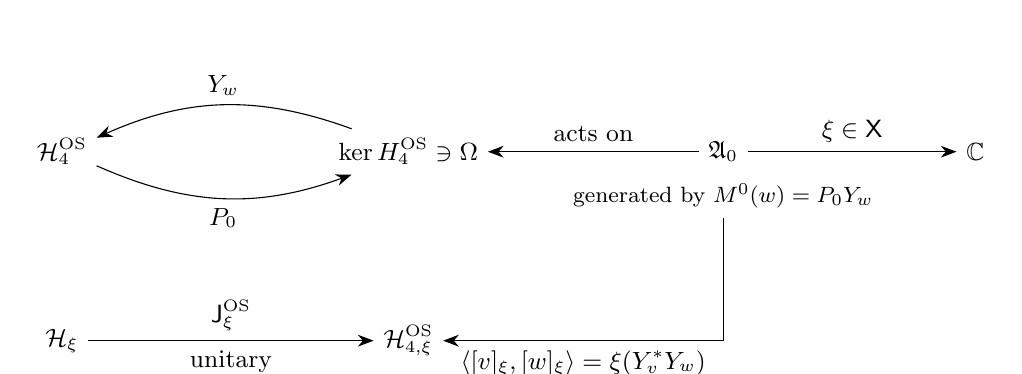
\begin{tikzpicture}[font=\small,>={Stealth[length=2mm]}]
\node (H) at (0,0) {$\mathcal H_4^{\rm OS}$};
\node (K) at (4.4,0) {$\ker H_4^{\rm OS}\ni\Omega$};
\node (A) at (8.4,0) {$\mathfrak A_0$};
\node[below=1pt of A,font=\footnotesize] (Ag) {generated by $M^0(w)=P_0Y_w$};
\node (C) at (11.6,0) {$\C$};
\draw[->] (K) to[bend right=22] node[above] {$Y_w$} (H);
\draw[->] (H) to[bend right=22] node[below] {$P_0$} (K);
\draw[->] (A) -- node[above] {acts on} (K);
\draw[->] (A) -- node[above] {$\xi\in\phases$} (C);
\node (Hx) at (4.4,-2.4) {$\mathcal H_{4,\xi}^{\rm OS}$};
\node (Hw) at (0,-2.4) {$\mathcal H_\xi$};
\draw[->] (Hw) -- node[above] {$\mathsf J_\xi^{\rm OS}$} node[below] {unitary} (Hx);
\draw[->] (Ag.south) |- node[pos=0.75,below] {$\langle[v]_\xi,[w]_\xi\rangle=\xi(Y_v^*Y_w)$} (Hx);
\end{tikzpicture}
\caption{The spaces and maps of this section. A positive word~$w$ in a slab gives the insertion $Y_w$ from the full ground space $\ker H_4^{\rm OS}$ of the mixture, which need not be a line, into its OS space; compression by the ground projection~$P_0$ gives~$M^0(w)$, and these operators generate the commutative algebra~$\mathfrak A_0$. A phase is a character~$\xi$ of~$\mathfrak A_0$. The OS space of the phase is the completion of positive words under the form $\xi(Y_v^*Y_w)$, the value of~$\xi$ on the compression of a whole word, which need not be the product of the values on its two halves~\eqref{eq:H-compression-defect}. Its ground space is a line for $\nu$-almost every phase by Lemma~\ref{lem:H1.3} and for every phase by Lemma~\ref{lem:H2.3}. The relativistic space~$\mathcal H_\xi$ of Section~\ref{sec:partII-H.2} is identified with it by the unitary map of Lemma~\ref{lem:H2.2}.}
\label{fig:H-spaces}
\end{figure}

\begin{figure}[t]
\centering
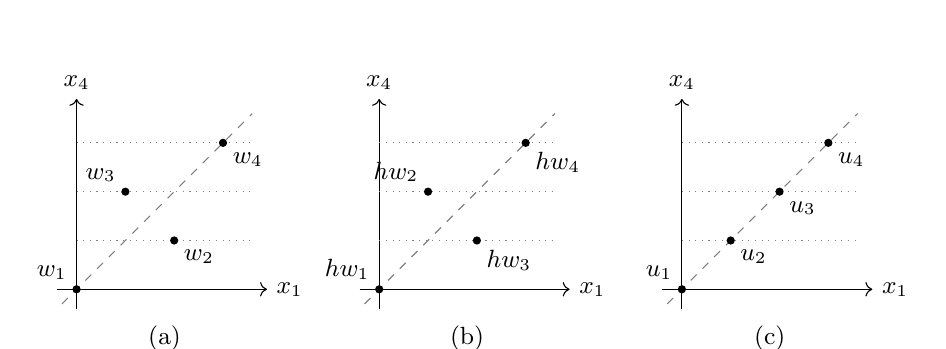
\begin{tikzpicture}[scale=0.62,font=\small]
\foreach \dx/\tag in {0/(a),6.2/(b),12.4/(c)}{
  \begin{scope}[xshift=\dx cm]
  \draw[->] (-0.4,0) -- (3.9,0) node[right] {$x_1$};
  \draw[->] (0,-0.4) -- (0,3.9) node[above] {$x_4$};
  \draw[dashed,gray] (-0.3,-0.3) -- (3.6,3.6);
  \foreach \t in {1,2,3}{\draw[dotted,gray] (0,\t) -- (3.6,\t);}
  \node at (1.8,-1.0) {\tag};
  \end{scope}}
\foreach \p/\l/\a in {(0,0)/w_1/above left,(2,1)/w_2/below right,(1,2)/w_3/above left,(3,3)/w_4/below right}{
  \fill \p circle (2.4pt) node[\a] {$\l$};}
\begin{scope}[xshift=6.2cm]
\foreach \p/\l/\a in {(0,0)/hw_1/above left,(2,1)/hw_3/below right,(1,2)/hw_2/above left,(3,3)/hw_4/below right}{
  \fill \p circle (2.4pt) node[\a] {$\l$};}
\end{scope}
\begin{scope}[xshift=12.4cm]
\foreach \k in {0,1,2,3}{\fill (\k,\k) circle (2.4pt);}
\node[above left] at (0,0) {$u_1$}; \node[below right] at (1,1) {$u_2$};
\node[below right] at (2,2) {$u_3$}; \node[below right] at (3,3) {$u_4$};
\end{scope}
\end{tikzpicture}
\caption{The axis exchange in the proof of Lemma~\ref{lem:H1.2}, in the plane of the first and fourth coordinates, in units of~$j$; time~$x_4$ is vertical, and the dashed line is fixed by the exchange~$h$. (a)~Four words, in time order $w_1,w_2,w_3,w_4$. (b)~After~$h$ the set of points is the same, but the transformed middle words have traded places, so the time order is $hw_1,hw_3,hw_2,hw_4$. (c)~On the diagonal, $h$ moves no point and changes no time order; this identity removes~$h$ from the products.}
\label{fig:H-exchange}
\end{figure}

Rotations make spatial translations trivial at zero energy; compression then removes slab width and placement.
\begin{lemma}[Compression algebra]\label{lem:H1.2}
The operators $M^0(w)$ are independent of the slab width and placement. They generate a separable commutative unital C$^*$-algebra~$\mathfrak A_0$ on $\ker H_4^{\rm OS}$, with cyclic and separating vector~$\Omega$. Its character space~$\phases$ is compact metric, the vacuum state is given by a full-support probability measure~$\nu$, and
\begin{equation*}
S^\xi(w)=\xi(M^0(w)),\qquad S(w)=\int_{\phases}\xi(M^0(w))\,d\nu(\xi)\,.
\end{equation*}
\end{lemma}
\begin{proof}
For fixed words and large~$z^4$ the correlation is $\langle v,U_{\vec z}e^{-(z^4-c)H_4^{\rm OS}}v'\rangle$, and strong heat convergence makes fixed time shifts negligible, uniformly in~$\vec z$. Choose an orthogonal reflection~$K$ taking $y+e_4$ to $|y+e_4|e_4$. Since $\langle K(y+e_4),Ke_4\rangle=1$, the ray $tKe_4$ has positive time component. By the covariance of Lemma~\ref{lem:G3.1}, rotating the displacements $te_4+y+e_4$ and~$te_4$ makes their difference purely temporal, so their correlations become equal in the limit; removing the extra~$e_4$ gives $U_yP_0=P_0$ by density.

The identities $\mathsf B_{h+t}(w)=\mathsf B_h(w)e^{-tH_4^{\rm OS}}$ and $\mathsf B_{h+t}(\tau_{te_4}w)=e^{-tH_4^{\rm OS}}\mathsf B_h(w)$ give width and placement independence of $M^0(w)$, and $M^0(w)\Omega=P_0[w]$, $\langle\Omega,M^0(w)\Omega\rangle=S(w)$. Successive use of~\eqref{eq:H-slab-laws} proves the cluster identity
\begin{equation}\label{eq:H-clusters}
\lim_{j\to\infty}S\bigl(\tau_{z_1(j)}w_1\cdots\tau_{z_m(j)}w_m\bigr)
=\langle\Omega,M^0(w_1)\cdots M^0(w_m)\Omega\rangle
\end{equation}
whenever $(z_{i+1}(j)-z_i(j))^4\to\infty$; in the induction, $\psi_j\to\psi$ and $t_j\to\infty$ imply $U_{y_j}e^{-t_jH_4^{\rm OS}}\psi_j\to P_0\psi$ for arbitrary~$y_j$.

\emph{Commutativity.} Let $h\in O(4)$ exchange the first and fourth coordinates, and write $hw$ for the word whose points, internal offsets included, and labels are transformed by~$h$, the labels through the representations of Lemma~\ref{lem:G3.1}. Place four words $w_1,\ldots,w_4$ at
\begin{equation*}
z_1=0,\quad z_2=j(e_4+2e_1),\quad z_3=j(2e_4+e_1),\quad z_4=3j(e_4+e_1),
\end{equation*}
with times $0,j,2j,3j$ (Figure~\ref{fig:H-exchange}). The points $hz_i$ have times $0,2j,j,3j$: the two middle words exchange their time order. Covariance and~\eqref{eq:H-clusters}, applied before and after~$h$, give
\begin{equation*}
\langle\Omega,M^0(w_1)M^0(w_2)M^0(w_3)M^0(w_4)\Omega\rangle
=\langle\Omega,M^0(hw_1)M^0(hw_3)M^0(hw_2)M^0(hw_4)\Omega\rangle .
\end{equation*}
The right side still carries~$h$. Words $u_k$ at the points $(k-1)j(e_4+e_1)$, $k=1,\ldots,4$, which $h$ fixes, keep their time order, so the same two identities give $\langle\Omega,\prod_kM^0(hu_k)\Omega\rangle=\langle\Omega,\prod_kM^0(u_k)\Omega\rangle$. With $(u_k)=(w_1,w_3,w_2,w_4)$ this removes~$h$:
\begin{equation*}
\langle\Omega,M^0(w_1)\bigl[M^0(w_2),M^0(w_3)\bigr]M^0(w_4)\Omega\rangle=0 .
\end{equation*}
The vectors $M^0(w_4)\Omega=P_0[w_4]$ span a dense subspace of $\ker H_4^{\rm OS}$. By~\eqref{eq:H-slab-laws}, the reflection $w_1=\theta v$ of a positive word~$v$ has $M^0(w_1)=M^0(v)^*$, so the vectors $M^0(w_1)^*\Omega=P_0[v]$ do too. Hence $M^0(w_2)$ and $M^0(w_3)$ commute. Density also gives cyclicity, and the empty word gives the unit. If $a\Omega=0$, then $ab\Omega=0$ on this span, so $a=0$. Basis labels and countable dense position sets generate~$\mathfrak A_0$ by norm continuity. Gelfand theory and the vacuum state give the compact metric spectrum and the probability measure~\cite[Theorems~2.4.1 and~2.8.2]{Landsman1998}; separation gives full support, since $\int|\xi(a)|^2d\nu=\|a\Omega\|^2$ vanishes only for $a=0$.
\end{proof}

Compression does not preserve products, and the identities used below have separate jobs. For a positive word~$v$ in a slab of width~$h$ put $Y_v=\mathsf B_h(v)|_{\ker H_4^{\rm OS}}$, a bounded map from $\ker H_4^{\rm OS}$ to~$\mathcal H_4^{\rm OS}$. Then $M^0(v)=P_0Y_v$, and~\eqref{eq:H-slab-laws} gives $M^0(\theta v\,w)=Y_v^*Y_w$ for the reflected whole word. For bounded operators $A,B$ and an orthogonal projection~$P_0$ one has $P_0ABP_0-(P_0AP_0)(P_0BP_0)=P_0A(1-P_0)BP_0$; here it reads
\begin{equation}\label{eq:H-compression-defect}
M^0(\theta v\,w)-M^0(v)^*M^0(w)=Y_v^*(1-P_0)Y_w\,.
\end{equation}
A character is multiplicative on~$\mathfrak A_0$, but a phase evaluates a word at finite separation through the compression of the whole word, $S^\xi(\theta v\,w)=\xi(Y_v^*Y_w)$. In the OS space of the phase, $\xi(M^0(v)^*M^0(w))=\langle[v]_\xi,\Omega_\xi^{\rm OS}\rangle\langle\Omega_\xi^{\rm OS},[w]_\xi\rangle$, so the character of the right side of~\eqref{eq:H-compression-defect} is the part of $\langle[v]_\xi,[w]_\xi\rangle$ orthogonal to the phase vacuum; it vanishes for all~$v,w$ only if that space is the line~$\C\Omega_\xi^{\rm OS}$. A long empty time interval between the two halves replaces $1-P_0$ by $e^{-tH_4^{\rm OS}}-P_0$, which tends to zero strongly. This is the mechanism of the cluster identity~\eqref{eq:H-clusters}, which produces products and hence commutativity; the whole-word identity $M^0(\theta v\,w)=Y_v^*Y_w$ produces the positivity of the phase OS form in Lemma~\ref{lem:H1.3}.

Moment bounds in the vacuum state bound a compressed operator in every phase. This is the form in which lattice chessboard estimates enter here and in Sections~\ref{sec:partII-I}--\ref{sec:partII-J}.
\begin{lemma}[Vacuum moments bound compressed operators]\label{lem:H-roots}
Let $U\in\mathfrak A_0$ and $B\ge0$ satisfy $\langle\Omega,(U^*U)^n\Omega\rangle\le B^{2n}$ for every $n\in\N$. Then $\|U\|=\sup_{\xi\in\phases}|\xi(U)|\le B$.
\end{lemma}
\begin{proof}
By Lemma~\ref{lem:H1.2}, $\langle\Omega,(U^*U)^n\Omega\rangle=\int|\xi(U)|^{2n}\,d\nu(\xi)$. If $|\xi_0(U)|>b>B$, continuity gives an open neighbourhood~$O$ of~$\xi_0$ on which $|\xi(U)|>b$, and full support gives $\nu(O)>0$. Then $\nu(O)b^{2n}\le B^{2n}$ for every~$n$, which is impossible. Gelfand theory identifies $\|U\|$ with $\sup_\xi|\xi(U)|$.
\end{proof}
The moment hypothesis comes from the lattice as follows. Let a lattice word difference be interior with centered chessboard seminorm at most~$B_0$ in one cell, multiplied by exterior insertions with centered chessboard seminorms at most $B_1,\ldots,B_L$ in disjoint finer cells, and let $U\in\mathfrak A_0$ be its compressed limit along the ordered limit. Apply~\eqref{eq:F-chess} to $2n$ widely translated copies, alternately conjugated; take the ordered limits and then infinite translation separation, using~\eqref{eq:H-clusters}; reflection identifies the alternating copies with adjoints. This gives $\langle\Omega,(U^*U)^n\Omega\rangle\le(B_0\prod_lB_l)^{2n}$, hence $\|U\|\le B_0\prod_lB_l$.

A generic grid word has positions in $a_k\Z^4$ with pairwise distinct coordinates along each axis. For real coefficient representatives~$(d_i,c_i)$ write $\langle\cdot\rangle_{N,p}$ for the Wilson expectation of Section~\ref{sec:wilson}, and put $\mathcal O_{N,p}(w)=\prod_i O^{(d_i)}_{N,p}(c_i,x_i/a_N)$. The word differences used below are
\begin{equation}\label{eq:H-real-approx}
f_{j,N,p,T}=\mathcal O_{N,p}(\tau_{z_j(T)}w)-\mathcal O_{N,p}(\tau_{z_j(T)}\vartheta w),\qquad z_j(T)=Tja_k(1,1,1,1).
\end{equation}
For each degree bound and lower grid level~$m$, Lemma~\ref{lem:E2-bounded-real} chooses $k\ge m$ before~$w$; these are the cofinal grids used below. For $\varepsilon>0$ it supplies real $g_{j,N,p,T}$ and a finite $R_\varepsilon$, independent of $N,p,T,j$, with $|g_{j,N,p,T}|\le R_\varepsilon$ eventually in the ordered cutoffs for each fixed~$T,j$, and, for $i<j$ and large~$T$, eventually in the ordered cutoffs, $|\langle g_ig_j\rangle_{N,p}-\operatorname{Re}\langle f_if_j\rangle_{N,p}|\le\varepsilon$; the threshold may depend on $T,i,j$. Bounded~$g_i$ control the diagonal variance terms, for which $f_i^2$ has no uniform bound.

\begin{lemma}[Phase fields and selection]\label{lem:H1.3}
For every $\xi\in\phases$, its table satisfies E1--E7, retains the inclusions, derivatives, conjugation, rotations and stress identities of the mixture, and
\begin{equation*}
\nullspace{d}(S^\xi)=\nullspace{d}(S)\qquad(d\in\N)\,.
\end{equation*}
Each separated value is continuous in~$\xi$. For $\nu$-almost every~$\xi$, the time-axis OS ground space is one-dimensional.
\end{lemma}
\begin{proof}
\emph{Reflection and rotation invariance.} We first prove
\begin{equation}\label{eq:H-reflection}
M^0(\vartheta w)=M^0(w),\qquad M^0(hw)=M^0(w)\quad(h\in O(4))\,.
\end{equation}
For a real grid word set $Z=M^0(w)-M^0(\vartheta w)$. Equation~\eqref{eq:H-slab-laws} gives $Z^*=-Z$, so $a=\langle\Omega,Z^2\Omega\rangle=-\|Z\Omega\|^2\le0$. Lattice variance gives
\begin{equation*}
0\le\left\langle\left(\sum_{i=0}^qg_i\right)^2\right\rangle
\le(q+1)R_\varepsilon^2+2\sum_{i<j}\left(\operatorname{Re}\langle f_if_j\rangle+\varepsilon\right)\,.
\end{equation*}
For fixed $q,T$, intersect the finitely many eventual sets, take the ordered cutoffs, then $T\to\infty$. Each pair expands into four separated moments, whose signed sum tends to~$a$ by Lemma~\ref{lem:E3.1}, \eqref{eq:F-conf} and~\eqref{eq:H-clusters}. Thus $0\le(q+1)[R_\varepsilon^2+q(a+\varepsilon)]$; first $q\to\infty$, then $\varepsilon\downarrow0$, gives $a\ge0$, and separation of~$\Omega$ gives $Z=0$. Grid density, norm continuity and multilinearity give all words. For the second identity, the cluster identity gives simultaneous orthogonal invariance of two-factor vacuum entries along rays with positive time before and after rotation; such a ray exists unless time is reversed, when composition with~$\vartheta$ suffices. With $v=M^0(u)\Omega$ and $x=M^0(w)\Omega$, simultaneous invariance and time-reflection invariance give $\langle v,x\rangle=\langle g^{-1}v,\vartheta g^{-1}x\rangle=\langle v,g\vartheta g^{-1}x\rangle$. Density gives every hyperplane reflection, and an orthogonal map is a product of at most four reflections.

\emph{Euclidean properties.} Testing on positive words gives the permutation, unit and linearity identities and annihilates mixed null labels, so $\nullspace{d}(S)\subset\nullspace{d}(S^\xi)$. Character evaluation gives reality, covariance and smooth phase values, continuous in~$\xi$. For positive words~$w_i$ in a common slab write $Y_i=Y_{w_i}\colon\ker H_4^{\rm OS}\to\mathcal H_4^{\rm OS}$. Since $M^0(\theta w_iw_j)=Y_i^*Y_j$,
\begin{equation*}
\sum_{i,j}\bar c_ic_jM^0(\theta w_iw_j)=\left(\sum_i c_iY_i\right)^*\left(\sum_jc_jY_j\right)\ge0\,.
\end{equation*}
The entries are compressions of whole words, not the products $M^0(w_i)^*M^0(w_j)$ (see~\eqref{eq:H-compression-defect}); a character applied to them gives a positive semidefinite matrix, which need not have rank one. Spectral permanence and character evaluation preserve positivity~\cite[Theorems~2.5.1(1) and~2.6.4]{Landsman1998}, and coordinate rotations give every axis; integrating the vectors of this positive Gram kernel against compact positive-time joint tests expresses the smeared OS form as a norm square. Inclusions and derivatives pass through bounded compression and character evaluation. To transfer the shell identities, extend the character $\xi$ by the complex Hahn--Banach theorem to a bounded linear functional $\widetilde\xi$ on $\mathcal B(\ker H_4^{\rm OS})$, and put
\[
 \ell_\xi(T)=\widetilde\xi(P_0T|_{\ker H_4^{\rm OS}}),
 \qquad T\in\mathcal B(\mathcal H_4^{\rm OS}).
\]
This is a fixed bounded linear functional; no positivity or multiplicativity of its extension is needed. On a slab insertion it evaluates the compressed whole word and hence gives $S^\xi$.

Fix a distinguished insertion, finitely many distinct spectators and an admissible smooth compactly supported shell cutoff $\chi$, equal to one near the distinguished point and supported away from the spectators. Translate the entire configuration and $\operatorname{supp}\chi$ into one slab with positive boundary margins. For each shell weight $q(y)$ occurring in Theorem~\ref{prop:ST}, including the linear rotational factor, multiply the slab operator with the stress inserted at $y$ by $q(y)$. The weight has compact support away from every insertion. Set the product to zero near the collision points; by the norm-smoothness in~\eqref{eq:H-slab-derivative} it is a continuous compactly supported $\mathcal B(\mathcal H_4^{\rm OS})$-valued function. Its Bochner integral exists, and $\ell_\xi$ commutes with that integral by bounded linearity.

Test the resulting operator integral against arbitrary positive-word vectors. Their reflected and translated exterior words lie outside the buffered slab, hence outside $\operatorname{supp}\chi$; the same cutoff is admissible with these extra spectators. The mixed shell identity gives the desired equality of all such matrix elements. Density and boundedness give an operator equality, and applying $\ell_\xi$ gives the phase shell identity with the same tensor and field maps. Absolute integrability of the phase scalar integrands follows from the norm bound on the compact support. Finally, $|S^\xi(w)|\le\|\mathsf B_h(w)\|$, also for derivative labels, gives E7 and separated-support integrability.

\emph{Equal null spaces.} This argument uses the corrected detector lifts and exact replicated moment bounds on the same selected family, including the equation and inclusion inputs of Lemmas~\ref{lem:E2.6}--\ref{lem:E2.10} and the fixed-period marked limit used by Lemma~\ref{lem:F2}. The equality of null spaces is conditional on those inputs; the bounded shell evaluator above is independent of this rank step. Use the rows of Lemma~\ref{lem:E2-free-tests}, corrected lifts of Lemma~\ref{lem:E2.10} and coefficient limits of Lemma~\ref{lem:F2}. Each row of trial~$\ell$ consists of a singleton~$u$ and optional spectator~$v$, placed at the comparison points $r_\ell y^{\ell,i}$. Write $\mathcal G_I^\ell$ for the Maxwell moment of the row labels in slots~$I$ at the unscaled points~$y^{\ell,i}$, and set $s=\mathcal G^\ell_{\{u\}}$, $s'=\mathcal G^\ell_{\{v\}}$ and $c=\mathcal G^\ell_{\{u,v\}}-ss'$, omitting terms with~$v$ in singleton rows. In~$\mathfrak A_0$ put
\begin{equation*}
\Delta_1=M^0(u)-s1,\quad\Delta_1'=M^0(v)-s'1,\quad
\Delta_2=M^0(uv)-sM^0(v)-s'M^0(u)+(ss'-c)1\,.
\end{equation*}
The polynomials of~\eqref{eq:F-relative} have centered chessboard seminorms at most $\gamma_\ell+\varepsilon$, preserved under signed images and conjugation by translating the periodic pattern; the lattice moment argument after Lemma~\ref{lem:H-roots}, followed by $\varepsilon\downarrow0$, gives
\begin{equation}\label{eq:H-moments}
\int_{\phases}|\xi(\Delta)|^{2j}\,d\nu(\xi)\le\gamma_\ell^{2j}\qquad(j\in\N)\,,
\end{equation}
and Lemma~\ref{lem:H-roots} gives $|\xi(\Delta_1)|,|\xi(\Delta_1')|,|\xi(\Delta_2)|\le\gamma_\ell$ in every phase. Expanding $\Delta_2$ gives $|\xi(M^0(uv))-ss'-c|\le\gamma_\ell(1+|s|+|s'|)$. The comparison has three parts of different kinds:
\begin{equation*}
\nullspace{d}(S)\subset\nullspace{d}(S^\xi),\qquad
\dim V_d/\nullspace{d}(S^\xi)\le\dim F_d=\dim\maxwellspace{d}\le\dim V_d/\nullspace{d}(S^\xi).
\end{equation*}
The inclusion is exact and was proved above, and with~\eqref{eq:F-dimension} it gives the first inequality. The last inequality is perturbative: the phase singleton and pair evaluations of the corrected lifts factor through $V_d/\nullspace{d}(S^\xi)$ and converge, by the bounds just proved, to the injective free row map, whose positive minimum on the unit sphere makes them eventually injective. Equal finite codimension and the inclusion give $\nullspace{d}(S^\xi)=\nullspace{d}(S)$.

\emph{Almost every ground space.} Reflection positivity and E7 construct the phase heat semigroup as in Lemma~\ref{lem:H1.1}. Write $[b]_\xi$ for a positive-word class and $P_{0,\xi}^{\rm OS}$ for its ground projection. Strong heat convergence and the mixture identity give, by dominated convergence,
\begin{equation*}
\int_{\phases}\|P_{0,\xi}^{\rm OS}[b]_\xi\|^2\,d\nu(\xi)
=\|P_0[b]\|^2=\int_{\phases}|S^\xi(b)|^2\,d\nu(\xi)\,,
\end{equation*}
the heat entries decreasing from their zero-time bounds. The integrands differ by $\|P_{0,\xi}^{\rm OS}[b]_\xi-S^\xi(b)\Omega_\xi^{\rm OS}\|^2$, which therefore vanishes almost everywhere. Rational configurations and basis coefficients give a countable dense family in every phase OS space, by Gram continuity; outside the union of its null sets the ground range is $\C\Omega_\xi^{\rm OS}$.
\end{proof}

Choose $\xi_*$ from the full-measure set of Lemma~\ref{lem:H1.3}; only its ground-space dimension enters this choice, and it is retained throughout. The slab bound passes to every phase with the same constants, by transferring the repeated insertion estimate through the character and applying the power argument of Lemma~\ref{lem:H1.1}.
\begin{corollary}[Phase slab operators]\label{cor:H-phase-slabs}\label{cor:H-phase-slab}
For every $\xi\in\phases$ the operators $A_w$ extend to bounded $\mathsf B_h^\xi(w)$ on $\mathcal H_{4,\xi}^{\rm OS}$ with $\|\mathsf B_h^\xi(w)\|\le\|\mathsf B_h(w)\|$, satisfying~\eqref{eq:H-slab-laws} and~\eqref{eq:H-slab-derivative}.
\end{corollary}
\begin{proof}
In the phase OS space put $v_j=(A_{w^\dagger}A_w)^jv$. The mixed-space map $Y(v_j)=\mathsf B(v_j)|_{\ker H_4^{\rm OS}}$ equals $(\mathsf B_h(w)^*\mathsf B_h(w))^jY(v)$, so $\|[v_j]_\xi\|^2=\xi(Y(v_j)^*Y(v_j))\le\|Y(v)\|^2\|\mathsf B_h(w)\|^{4j}$. The power argument gives $\mathsf B_h^\xi(w)$ of norm at most $\|\mathsf B_h(w)\|$, and the dense-vector argument gives its identities and norm derivatives.
\end{proof}

\begin{proof}[Proof of Theorem~\ref{prop:PH}]
Lemma~\ref{lem:H1.2} gives the character space, the full-support probability measure and the mixture formula. Lemma~\ref{lem:H1.3} gives E1--E7, equal null spaces, the common identities of Proposition~\ref{prop:FC} and Theorem~\ref{prop:ST}, covariance and phase continuity.
\end{proof}

\subsection{Reconstruction}\label{sec:partII-H.2}

Coordinates are indexed with time fourth, so $x^4$ is time and $\vec x$ is the spatial part. In the local Wick-slice argument of Lemma~\ref{lem:H-locality}, tuples are displayed with the time component first.

Use the response labels~$\mathcal L$ of Definition~\ref{def:D10}. With time reflection acting on labels through~$R_d$, the star is
\begin{equation}\label{eq:H-star}
(\iota_dA)^*=\iota_d\bigl(R_d(\mathsf s_4^{\rm refl})\overline A\bigr)\,.
\end{equation}
The boost generators $-i\mathsf L_d(K_{4i})$ and the spatial rotations integrate to $SL(2,\C)$, the simply connected cover of $SO^+(1,3)$; a full spatial turn acts trivially, so the action descends to $SO^+(1,3)$. Inclusions intertwine the actions, and the time-reflection sign of $K_{4i}$ and antilinearity make the star~\eqref{eq:H-star} commute with boosts. Take $\mathcal P=SO^+(1,3)\ltimes\R^4$ itself in Definition~\ref{def:D14b}, and $\rho_{\rm lab}(\Lambda,z)$ the continued label action of~$\Lambda$. Let $\mathfrak B$ be the Borchers algebra of finite sequences $F=(F_0,F_1,\ldots)$, $F_n\in\mathcal L^{\otimes n}\otimes\mathcal S_n$; its product concatenates label tensors and tensors the tests, and its antilinear star reverses order, applies the star~\eqref{eq:H-star} to labels and complex conjugation to tests. For a phase write $U_y^\xi$ for spatial translation on~$\mathcal H_{4,\xi}^{\rm OS}$, and put
\begin{equation*}
\mathcal V_n=\Bigl\{p\in(\R^4)^n:\sum_jp_j=0,\quad \sum_{k=j}^np_k\in\forwardcone\ (j\ge2)\Bigr\}\,.
\end{equation*}

Fix a phase~$\xi$. The reconstruction follows the scheme of Osterwalder and Schrader~\cite{OsterwalderSchrader1973,OsterwalderSchrader1975}, with one change: in place of their growth condition, the slab bounds of Lemma~\ref{lem:H1.1} and Corollary~\ref{cor:H-phase-slab} give the strip bound~\eqref{eq:H-poly}, from which the boundary distributions are obtained directly. Lemma~\ref{lem:H2.1} constructs the continuation and the boundary distributions, with covariance, spectral support, positivity, continuity in~$\xi$ and the barycenter formula. Lemma~\ref{lem:H-locality} proves locality, Lemma~\ref{lem:H-fields} realizes the fields, Lemma~\ref{lem:H2.2} compares the Hilbert spaces, Lemma~\ref{lem:H2.3} proves the uniform low-energy bound and vacuum uniqueness, Lemma~\ref{lem:H-irreducible} proves irreducibility, and Lemma~\ref{lem:H2.4} continues the stress tensor.

The requirements of Theorem~\ref{prop:RC} come from three sources. Reflection positivity gives the OS spaces, their heat semigroups and the positivity of the boundary distributions. Slab growth gives bounded insertions, hence the strip bound, tempered boundary values and continuity in the phase. The rotations of Lemma~\ref{lem:G3.1}, continued to boosts, give Lorentz covariance and, through imaginary boosts, locality. Vacuum uniqueness first holds only for $\nu$-almost every phase (Lemma~\ref{lem:H1.3}). The low-energy estimate of Lemma~\ref{lem:H2.3} is uniform in the phase; with the continuity in~$\xi$ of the vacuum-subtracted heat pairings and the full support of~$\nu$, it removes the exceptional set. That estimate, $\mu_{A\Omega_\xi}\{0<E\le u\}\le M_Au^2$, is polynomial in the energy: no positive lower bound on nonzero energies (spectral gap) is used or proved. Vacuum uniqueness is a statement inside one phase; nothing here shows that~$\nu$ is a point mass.

Positive-height operators give positive boundary distributions without a Euclidean extension across collisions.
\begin{lemma}[Continuation and boundary distributions]\label{lem:H2.1}
For every $\xi\in\phases$ and label list~$a$, the functions $\mathsf F^\xi_n(a;\cdot)$ of~\eqref{eq:H-continuation} satisfy Definition~\ref{def:D15}, and their boundary values in Definition~\ref{def:D14f} define joint Schwartz distributions $W^\xi_n(a;\psi)$, bounded by one Schwartz seminorm uniformly in~$\xi$. These are Poincar\'e covariant for the label action above, their Fourier transforms are supported in~$\mathcal V_n$, and $W^\xi(F^*F)\ge0$ for $F\in\mathfrak B$. Each $\xi\mapsto W^\xi_n(a;\psi)$ is continuous, and $\int_{\phases}W^\xi_n(a;\psi)\,d\nu(\xi)=W^{\rm mix}_n(a;\psi)$.
\end{lemma}
Here $W^{\rm mix}_n$ is the boundary distribution of the mixed continuation, defined below.
\begin{proof}
\emph{Positive imaginary times.} Write $e^{-tH_{4,\xi}^{\rm OS}}$ for the phase heat semigroup. For a label~$a$ put $B_{\xi,\epsilon}(a)=\mathsf B_{2\epsilon}^\xi(a(\epsilon e_4))$; Lemma~\ref{lem:H1.1} and Corollary~\ref{cor:H-phase-slab} give $\|B_{\xi,\epsilon}(a)\|\le C_a\epsilon^{-q_a}$ for $0<\epsilon<1$, uniformly in~$\xi$. For $\operatorname{Im}z>2\epsilon$ set $G_{\xi,\epsilon}(z,y)=e^{-(\operatorname{Im}z-2\epsilon)H_{4,\xi}^{\rm OS}}e^{i\operatorname{Re}zH_{4,\xi}^{\rm OS}}U_y^\xi$, and for $n\ge1$
\begin{equation}\label{eq:H-continuation}
\mathsf F_n^\xi(a;z,\vec x)=\langle\Omega_\xi^{\rm OS},B_{\xi,\epsilon}(a_1)
\prod_{j=2}^n\bigl[G_{\xi,\epsilon}(z_j-z_{j-1},\vec x_j-\vec x_{j-1})B_{\xi,\epsilon}(a_j)\bigr]\Omega_\xi^{\rm OS}\rangle\,,
\end{equation}
with $0<\epsilon<1$ and $4\epsilon<\min_j\operatorname{Im}(z_{j+1}-z_j)$; set $\mathsf F_0^\xi=1$. At imaginary times the insertion rule gives~$S_n^\xi$, independently of~$\epsilon$, and the identity theorem extends this agreement. The function is holomorphic in the times and continuous in space; extend it by zero outside ordered times. Taking $\epsilon=\delta/8$ gives, uniformly in~$x$ and~$\xi$,
\begin{equation}\label{eq:H-poly}
|\mathsf F_n^\xi(a;x^4+iy,\vec x)|\le C\delta^{-m}
\quad\left(0<\delta\le1,\ y_{j+1}-y_j\ge\delta\right).
\end{equation}

\emph{Boundary distributions.} Write $\phi_\xi(y;f)=\int\mathsf F_n^\xi(a;x^4+iy,\vec x)f(x)\,dx$ and $\mathcal G=-i\sum_jj\,\partial_{x_j^4}$. By~\eqref{eq:H-poly} and holomorphy, integration by parts gives $\partial_t\phi_\xi(y+t\varrho;f)=\phi_\xi(y+t\varrho;\mathcal Gf)$ with $\varrho_j=j$, and repeated integration gives
\begin{equation}\label{eq:H-boundary}
\phi_\xi(y;f)=\sum_{k=0}^m\frac{(-1)^k}{k!}\phi_\xi(y+\varrho;\mathcal G^kf)
-\int_0^1\frac{(-t)^m}{m!}\phi_\xi(y+t\varrho;\mathcal G^{m+1}f)\,dt\,.
\end{equation}
The integrand is bounded by $C\|\mathcal G^{m+1}f\|_{L^1}/m!$, uniformly in~$y,\xi$. At $y=0$ this defines~$W_n^\xi$, and dominated convergence gives every ordered boundary limit and a common Schwartz seminorm bound.

\emph{Dependence on the phase.} The mixed operators of Lemma~\ref{lem:H1.1} define $\mathsf F^{\rm mix}$ by~\eqref{eq:H-continuation} and $W^{\rm mix}$ by~\eqref{eq:H-boundary}, with the same bound. The mixture formula at imaginary times extends to strict times by the identity theorem and integration of Cauchy's formula. For continuity set $z_j=iy_j+\varsigma x_j^4$; the common strip bound gives a normal family in~$\varsigma$, and if $\xi_\ell\to\xi$, each subsequential limit agrees on the imaginary segment by Lemma~\ref{lem:H1.3}, hence everywhere. Fubini and the common integrable bound in~\eqref{eq:H-boundary} give continuity of the distributions and the barycenter formula.

\emph{Lorentz covariance.} Display the $j$th label in $\phi_\xi(y;f;\ldots,a_j,\ldots)$. Differentiating Euclidean $(4,i)$ covariance and using the time Cauchy--Riemann identity gives
\begin{equation*}
\sum_j\phi_\xi(y;f;\ldots,-i\mathsf L(K_{4i})a_j,\ldots)
=\phi_\xi\Bigl(y;\sum_j[x_j^i\partial_{x_j^4}+(x_j^4+iy_j)\partial_{x_j^i}]f\Bigr),
\end{equation*}
first at imaginary times, then by holomorphy. At the boundary~\eqref{eq:H-boundary} removes~$y$, so along a real boost the derivative of simultaneously transformed labels and tests is zero. Spatial rotations and translations keep their Euclidean identities.

\emph{Spectral support.} Define $\widetilde W_n^\xi(b)=W_n^\xi(\fourierplus{b}(-\cdot))$. For compactly supported smooth frequency tests~$b$, differentiating the height and the exponential multiplier gives cancellation, hence
\begin{equation}\label{eq:H-Laplace}
\widetilde W_n^\xi(b)=\phi_\xi\bigl(y;\fourierplus{(e^{\sum_jy_jp_j^4}b)}(-\cdot)\bigr)\,,
\end{equation}
including the zero endpoint. Sending ordered heights to infinity kills negative time-tail momenta, and translation and Lorentz covariance give support in~$\mathcal V_n$.

\emph{Positivity.} Apply the propagators and insertions in~\eqref{eq:H-continuation} to the vacuum, with an initial heat interval, and smear against a word test~$b$. Reflection and the insertion rule identify mixed-height Gram entries with $\mathsf F^\xi(b^*c)$, whose limits as both height lists vanish are $W^\xi(b^*c)$ by~\eqref{eq:H-boundary}. The vectors are therefore Cauchy, and their limits $v_\xi(b)\in\mathcal H_{4,\xi}^{\rm OS}$ have this Gram form; the common seminorm bound and product-test density extend it to joint tests. Hence $W^\xi(F^*F)=\|\sum_b c_bv_\xi(b)\|^2\ge0$.
\end{proof}

Locality is the exchange of two adjacent spacelike points. For $1\le j<n$ let $s$ be the transposition of $j$ and $j+1$, write $x^s$ and $a^s$ for configurations and label lists with these entries exchanged, and put $\mathcal G_j=\{x\in(\R^4)^n:\minksquare(x_{j+1}-x_j)<0\}$.
\begin{lemma}[Exchange of adjacent spacelike points]\label{lem:H-locality}
For every $\xi\in\phases$, label list~$a$, $1\le j<n$ and $\psi\in\mathcal S_n$ supported in~$\mathcal G_j$,
\begin{equation*}
W^\xi_n(a;\psi)=W^\xi_n(a^s;\psi^s),\qquad \psi^s(x)=\psi(x^s).
\end{equation*}
\end{lemma}
The two orders give two holomorphic functions on two different tubes. Opposite imaginary boosts move a configuration with tied heights into the two tubes and so define two holomorphic germs at that configuration. At zero real times both germs restrict to the same Euclidean correlation, by permutation symmetry, so they coincide; the equality is carried to arbitrary real times, and partial boundary values give the claim.
\begin{proof}
\emph{The tube function.} Let $\mathcal T_n=\{w\in(\C^4)^n:\operatorname{Im}(w_{k+1}-w_k)\in\openforwardcone,\ k<n\}$, where $\openforwardcone$ is the interior of~$\forwardcone$. Let $\chi=\mathbf1_{\{\operatorname{dist}(p,\mathcal V_n)<2\}}*\varrho_1$ with $\varrho_1\ge0$ smooth, of unit integral and supported in the unit ball; then $\chi=1$ near~$\mathcal V_n$, has bounded derivatives, and vanishes at distance greater than three. For $w\in\mathcal T_n$ define
\begin{equation*}
\mathcal W_a(w)=(2\pi)^{-4n}\widetilde W_n^\xi\bigl(\chi(p)e^{i\sum_kp_k\cdot w_k}\bigr).
\end{equation*}
With $q_k=\sum_{l\ge k}p_l$, one has $\sum_kp_k\cdot\operatorname{Im}w_k=\sum_{k\ge2}q_k\cdot\operatorname{Im}(w_k-w_{k-1})\ge c|p|$ on~$\mathcal V_n$, and up to a bounded subtraction on $\operatorname{supp}\chi$; so the test is a holomorphic family of Schwartz functions and $\mathcal W_a$ is holomorphic on~$\mathcal T_n$. By~\eqref{eq:H-Laplace}, $\mathcal W_a(w)=\mathsf F^\xi_n(a;w^4,\vec w)$ when the imaginary parts are purely temporal and strictly ordered; in particular $\mathcal W_a$ equals $S^\xi_n(a;\cdot)$ at ordered Euclidean points $w_k=(it_k,\vec x_k)$. For nondecreasing heights~$y$, the damping multiplier is $e^{-\sum_ky_kp^4_k}=e^{-\sum_{k\ge2}(y_k-y_{k-1})q_k^4}$ on the total-momentum hyperplane. Multiplying by the thickened-cone cutoff $\chi$ gives a smooth multiplier with bounded derivatives, locally uniformly in the heights: the tail energies are bounded below up to a fixed additive constant and total momentum is bounded on $\operatorname{supp}\chi$. It therefore maps Schwartz tests continuously to Schwartz tests. This defines partial boundary distributions $W^\xi_{n,y}(a;\cdot)$, continuous in~$y$, equal to $W^\xi_n(a;\cdot)$ at $y=0$, and equal to $\int\mathcal W_a(x+iy)f(x)\,dx$ for strictly increasing~$y$. Here $x+iy$ means $(x_k^4+iy_k,\vec x_k)_k$.

\emph{Complex boosts.} Real Lorentz covariance in Lemma~\ref{lem:H2.1} gives $\mathcal W_a(\Lambda w)=\rho_n^\vee(\Lambda)\mathcal W_a(w)$ for real~$\Lambda$ and $w\in\mathcal T_n$, where $\rho_n^\vee$ acts on label tensors. For a spatial unit vector~$e$ and rapidity~$\beta$, the label action of the boost $\Lambda_\beta$ along~$e$ is $\exp(-i\beta\sum_ie_i\mathsf L(K_{4i}))$ on finite-dimensional spaces, an entire function of~$\beta$. Hence the covariance identity holds for complex $\beta$, by the identity theorem in~$\beta$, whenever $\Lambda_{\beta'}w\in\mathcal T_n$ along a path from $0$ to~$\beta$.

\emph{Two germs.} Fix heights with $y_j=y_{j+1}$ and $y_k<y_{k+1}$ for the other~$k$, and $x\in\mathcal G_j$, so $w_0=x+iy$ lies on the boundary of~$\mathcal T_n$. Write $x_{j+1}-x_j=(\tau,\vec v)$ with $|\tau|<|\vec v|$ and put $e=\vec v/|\vec v|$. The imaginary boost $\Lambda_{ib}$ along~$e$ gives this difference the imaginary part $\sin b\,(|\vec v|,\tau e)$, in time and space components, which lies in~$\openforwardcone$ for $0<b<\pi$; for small~$b$ the other differences stay in~$\openforwardcone$. So, for a small $b_0>0$ and a small neighbourhood~$N$ of~$w_0$, $\Lambda_{ib_0}w\in\mathcal T_n$ for $w\in N$, and $\Lambda_{ib}w\in\mathcal T_n$ for $0\le b\le b_0$ if moreover $w\in\mathcal T_n$; the opposite boost $\Lambda_{-ib}$ moves the exchanged configuration into~$\mathcal T_n$. Define, near~$w_0$,
\begin{equation*}
G_+(w)=\rho_n^\vee(\Lambda_{ib_0})^{-1}\mathcal W_a(\Lambda_{ib_0}w),\qquad
G_-(w)=\rho_n^\vee(\Lambda_{-ib_0})^{-1}\mathcal W_{a^s}\bigl((\Lambda_{-ib_0}w)^s\bigr).
\end{equation*}
Both are holomorphic in a neighbourhood of~$w_0$. By the complex boost identity along $[0,b_0]$, $G_+=\mathcal W_a$ on the part of that neighbourhood in~$\mathcal T_n$, and $G_-(w)=\mathcal W_{a^s}(w^s)$ where $w^s\in\mathcal T_n$.

\emph{The Wick slice.} Suppose first that all real times of~$x$ vanish. Then $w_0=(iy_k,\vec x_k)_k$ is a separated Euclidean configuration, since $\vec x_j\ne\vec x_{j+1}$. The Wick slice $\{(it_k,\vec x_k)\}$ is a real subspace of dimension $4n$ whose complex span is $(\C^4)^n$. Near~$w_0$ on the slice, points with $t_j<t_{j+1}$ lie in~$\mathcal T_n$, where $G_+=S^\xi_n(a;\cdot)$; points with $t_j>t_{j+1}$ have exchanged configuration in~$\mathcal T_n$, where $G_-=S^\xi_n(a^s;(\cdot)^s)=S^\xi_n(a;\cdot)$ by permutation symmetry. Since $S^\xi_n$ is smooth at~$w_0$, all jets of $G_+$ and $G_-$ along the slice at~$w_0$, computed as limits from these open half-spaces, equal those of $S^\xi_n(a;\cdot)$. Real jets along the slice are restrictions of complex jets, and the slice spans $(\C^4)^n$; so all complex derivatives of $G_+-G_-$ vanish at~$w_0$, and $G_+=G_-$ near~$w_0$.

\emph{Propagation.} For general $x\in\mathcal G_j$ consider $x(t)=(tx_k^4,\vec x_k)_k$, $t\in[0,1]$; it stays in~$\mathcal G_j$, since $|t\tau|\le|\tau|<|\vec v|$, and the strict height margins persist. Along this compact path both germs are defined at every point. Two germs of the same kind at nearby points agree on the overlap of their domains, since both extend the same function from the open set $\mathcal T_n$ (respectively its exchanged image), which accumulates at each point. A finite chain of overlapping neighbourhoods carries $G_+=G_-$ from $t=0$ to $t=1$.

\emph{Partial boundary values.} For $f$ supported in a small ball around $x\in\mathcal G_j$, the representation of $W^\xi_{n,y}$ by the tube function and continuity up to the tied heights give $W^\xi_{n,y}(a;f)=\int G_+(x'+iy)f(x')\,dx'$, and likewise $W^\xi_{n,y^s}(a^s;f^s)=\int G_-(x'+iy)f(x')\,dx'$. These agree, and a partition of unity gives $W^\xi_{n,y}(a;\psi)=W^\xi_{n,y^s}(a^s;\psi^s)$ for compactly supported $\psi$ with support in~$\mathcal G_j$; for general $\psi\in\mathcal S_n$ with support in~$\mathcal G_j$, multiply $\psi$ by cutoffs equal to one on growing balls; these products converge to $\psi$ in~$\mathcal S_n$ without enlarging the support. Let the heights tend to zero along such tied height lists; continuity of the partial boundary distributions gives the claim.
\end{proof}

\begin{lemma}[Relativistic fields]\label{lem:H-fields}
For every $\xi\in\phases$, the boundary distributions of Lemma~\ref{lem:H2.1} define a faithful theory on~$\mathcal L$ satisfying W1--W3 and the spectral representation and spectral condition $\mathsf E(\R^4\setminus\forwardcone)=0$ of W0, with continuation the functions $\mathsf F^\xi_n$ of that lemma. Its adjoint and Lorentz label maps are the common maps specified above.
\end{lemma}
\begin{proof}
Complete the form $W^\xi(F^*G)$ on~$\mathfrak B$ modulo null vectors to obtain~$\mathcal H_\xi$, with $\Phi_\xi(a,f)[b]=[(a,f)b]$. For null~$x$ the inserted vector pairs with~$c$ as $\langle x,(a^*,\bar f)c\rangle=0$; taking $c$ to be that vector preserves nullity and gives the adjoint law W1. Test continuity gives strongly continuous covariance unitaries, and Lemma~\ref{lem:H2.1} gives W2. Translations integrate to a nondegenerate representation of $C^*(\R^4)=C_0(\R^4)$~\cite[Theorem~3.7.11 and equation~(3.89)]{Landsman1998} with joint spectral measure $\mathsf E$ from~\cite[Proposition~4.2.3]{Landsman1998}. To obtain its support, take $\eta\in C_c^\infty(\R^4\setminus\forwardcone)$ and a Schwartz function $k$ with $\int k(z)e^{iq\cdot z}\,dz=\eta(q)$. For word vectors $[b],[c]$, integrate $\langle[b],\mathsf T_\xi(z)[c]\rangle$ against $k(z)$. The spectral representation gives $\langle[b],\eta(\mathsf P)[c]\rangle$, where $\eta(\mathsf P)=\int\eta(q)\,d\mathsf E(q)$. In the Fourier convention of~\eqref{eq:H-Laplace}, translating the final word multiplies the joint test by $e^{iz\cdot q}$, where $q$ is the sum of that word's momenta. The integral therefore inserts $\eta(q)$ in the joint Schwartz test. If both words are nonempty and $|b|=m$, this is the tail $q=\sum_{k=m+1}^n p_k$; it belongs to $\forwardcone$ on $\mathcal V_n$. If the final word is empty then $q=0$, while if the first word is empty the total-momentum condition gives $q=0$. Since the compact support of $\eta$ is separated from the closed cone, the joint test vanishes on an open neighborhood of $\mathcal V_n$. The Fourier support of Lemma~\ref{lem:H2.1} makes the pairing zero. Density of word vectors gives $\eta(\mathsf P)=0$; such tests and regularity of the spectral measure give $\mathsf E(\R^4\setminus\forwardcone)=0$, without a vacuum-uniqueness assumption.

Lemma~\ref{lem:H-locality}, applied to adjacent pairs inside vacuum expectations of words, gives W3 on the word domain. The boundary condition of Definition~\ref{def:D14f} is the definition of~$W^\xi_n$ in Lemma~\ref{lem:H2.1}. If a label acts as zero for every test, all boundary word pairings with that insertion vanish. The strictly ordered imaginary-height form of~\eqref{eq:H-Laplace} then gives zero separated Euclidean correlations; symmetry and continuity cover all separated configurations. Lemma~\ref{lem:H1.3} and injectivity of responses give faithfulness.
\end{proof}

Surjectivity of the comparison map transfers ground-space information between the two Hilbert spaces.
\begin{lemma}[OS comparison]\label{lem:H2.2}
For every~$\xi$, there is a unique linear isometry $\mathsf J_\xi^{\rm OS}:\mathcal H_\xi\to\mathcal H_{4,\xi}^{\rm OS}$ with the boundary-word values specified before Theorem~\ref{prop:RC}. It is surjective, hence unitary, and intertwines spatial translations and the heat semigroups: $\mathsf J_\xi^{\rm OS}e^{-sH_\xi}=e^{-sH_{4,\xi}^{\rm OS}}\mathsf J_\xi^{\rm OS}$ for $s\ge0$.
\end{lemma}
\begin{proof}
The map $J:[b]\mapsto v_\xi(b)$ of Lemma~\ref{lem:H2.1} is an isometry taking vacuum to vacuum and intertwines spatial translations and heat by~\eqref{eq:H-Laplace}. Two linear isometries with these boundary-word values agree on the dense word span, hence everywhere. For compact frequency~$b$ let $f_y=\fourierplus{(e^{-\sum_jy_jp_j^4}b)}(-\cdot)$; by~\eqref{eq:H-Laplace} the norms and mixed pairing of its boundary-word image under~$J$ and the corresponding positive-height OS vector agree, so the two vectors coincide. Frequency-test density and closed range include every smeared positive-height vector, approximate identities give point vectors, and permutation and perturbation of equal times give all positive words. So $J$ is surjective.
\end{proof}

The low-energy estimate is the infrared input of the reconstruction. For a fixed compactly supported local word~$A$, locality makes a commutator vanish outside a bounded spatial region for bounded times. An odd time average turns this into a positive spectral weight comparable to the energy~$E$ near zero. A momentum cutoff at scale~$u$ costs~$u^3$ in three spatial dimensions, and the cone $|\vec p|\le E$ gives $u\,\mu\{u/2<E\le u\}\lesssim u^3$; dyadic summation gives~$u^2$.
\begin{lemma}[Uniform low-energy bounds and vacuum uniqueness]\label{lem:H2.3}
For every finite complex combination~$A$ of field words smeared with compactly supported smooth tests, there are $M_A,M'_A\ge0$, depending on its words, labels and tests, such that for every~$\xi\in\phases$,
\begin{align*}
\mu_{A\Omega_\xi}(\{0<\mathbf p^4\le u\})&\le M_Au^2&&(0<u\le1),\\
0\le\langle A\Omega_\xi,(e^{-sH_\xi}-P_{0,\xi})A\Omega_\xi\rangle&\le M'_As^{-2}&&(s\ge1),
\end{align*}
where $P_{0,\xi}$ projects onto~$\C\Omega_\xi$. Moreover $\ker H_\xi=\C\Omega_\xi$ and $\ker H_{4,\xi}^{\rm OS}=\C\Omega_\xi^{\rm OS}$.
\end{lemma}
\begin{proof}
\emph{The low-energy measure.} Let $Q_\xi=\mathsf E_\xi(\{\mathbf p^4=0\})$ be the full zero-energy projection; until the last step its range is not assumed to be a line. Let $A^*$ be the word adjoint, reversing order and applying the star~\eqref{eq:H-star} to labels and complex conjugation to tests, and put $\alpha_zA=\mathsf T_\xi(z)A\mathsf T_\xi(z)^*$. Bound all support times and spatial norms by~$r$ and set $R=4r+1$, $\mu=\mu_{A\Omega_\xi}$ and $\mu^*=\mu_{A^*\Omega_\xi}$. The common distribution bounds give $\mu(\R^4)+\mu^*(\R^4)\le M$, uniformly in~$\xi$. Covariance and locality give
\begin{equation*}
a(y,t)=\fourierplus{\mu}(y,t)-\fourierplus{\mu^*}(-y,-t)
=\langle\Omega_\xi,[A^*,\alpha_{(y,t)}A]\Omega_\xi\rangle=0
\quad(|y|>R,\ |t|\le1)\,,
\end{equation*}
with $\fourierplus{\mu}(z)=\int e^{ip\cdot z}\,d\mu(p)$. Write $E=p^4$. The time average $\bar a(y)=\int_0^1[a(y,t)-a(y,-t)]/(2i)\,dt$ is bounded by~$M$ and supported in~$\overline B_R$. It is the Fourier transform of two positive measures, the pushforwards of $\varpi(E)\,d\mu$ under $p\mapsto\vec p$ and of $\varpi(E)\,d\mu^*$ under $p\mapsto-\vec p$, where $\varpi(E)=(1-\cos E)/E$, $\varpi(0)=0$; on $0\le E\le1$, $\varpi(E)\ge E/\pi$. Choose a smooth momentum bump $b_u$ with $0\le b_u\le1$, equal to one on $B_u$ and supported in~$B_{2u}$; $|\fourierplus{b_u}(-y)|\le8|B_1|u^3$. Since $|\vec p|\le E$ on the spectral cone, $b_u=1$ on the shell $\{u/2<E\le u\}$, and Fourier inversion and positivity give
\begin{equation*}
(2\pi)^3\frac{u}{2\pi}\,\mu(\{u/2<E\le u\})
\le\left|\int\bar a(y)\fourierplus{b_u}(-y)\,dy\right|
\le8|B_1||B_R|M u^3\,.
\end{equation*}
Summing the shells at $u2^{-j}$ gives
\begin{equation}\label{eq:H-low}
\mu(\{0<E\le u\})\le C R^3M u^2\qquad(0<u\le1)\,.
\end{equation}
For $u>1$ use the total mass. Since $e^{-sE}=\int_E^\infty se^{-st}\,dt$, Tonelli gives
\begin{equation}\label{eq:H-heat}
0\le\langle A\Omega_\xi,(e^{-sH_\xi}-Q_\xi)A\Omega_\xi\rangle
=\int_{E>0}e^{-sE}\,d\mu
\le C_A s\int_0^\infty t^2e^{-st}\,dt=2C_As^{-2}\,.
\end{equation}

\emph{From almost every phase to every phase.} By Lemma~\ref{lem:H2.2}, $\mathsf J^{\rm OS}_\xi$ is unitary and intertwines heat, so it identifies $\ker H_\xi$ with $\ker H^{\rm OS}_\xi$; by Lemma~\ref{lem:H1.3} both are $\C\Omega_\xi$ for $\nu$-almost every~$\xi$, and there $Q_\xi=P_{0,\xi}$. The vacuum-subtracted heat pairing $\langle A\Omega_\xi,e^{-sH_\xi}A\Omega_\xi\rangle-|\langle\Omega_\xi,A\Omega_\xi\rangle|^2$ is continuous in~$\xi$: by~\eqref{eq:H-boundary} it is a continuous Schwartz pairing, with error $Me^{-sN}$ outside radius~$2N$ on~$\forwardcone$. It is bounded by $2C_As^{-2}$ for almost every~$\xi$, hence, by continuity and full support of~$\nu$, for every~$\xi$. Letting $s\to\infty$ gives $\|Q_\xi A\Omega_\xi\|^2=|\langle\Omega_\xi,A\Omega_\xi\rangle|^2$. Since $Q_\xi\Omega_\xi=\Omega_\xi$, density of compact word vectors gives $Q_\xi=P_{0,\xi}$, and~\eqref{eq:H-heat} becomes the second bound. Unitarity and heat intertwining give the OS vacuum line.
\end{proof}

\begin{lemma}[Irreducibility]\label{lem:H-irreducible}
For every~$\xi$, a bounded operator~$B$ is scalar if and only if, for every smeared field~$\Phi$ and $u,v\in\mathcal D_\xi$, one has $u\in\operatorname{Dom}\Phi^*$ and $\langle\Phi^*u,Bv\rangle=\langle u,B\Phi v\rangle$.
\end{lemma}
\begin{proof}
A scalar satisfies the relation by the adjoint law. Conversely, the adjoint law and iteration move words across matrix entries without requiring $B$ to preserve the domain. For a word~$A$ put $u=A\Omega_\xi$, $v=A^*\Omega_\xi$ and, in the upper half-plane,
\begin{equation*}
p(z)=\langle u,e^{izH_\xi}B\Omega_\xi\rangle,\qquad
q(z)=\langle B^*\Omega_\xi,e^{izH_\xi}v\rangle\,.
\end{equation*}
These are bounded and continuous to the boundary, where covariance and the weak relation give $p(t)=q(-t)$. Morera and Liouville make their bounded pasted continuation constant, so $\langle u,e^{-sH_\xi}B\Omega_\xi\rangle=\langle u,B\Omega_\xi\rangle$. Heat convergence and Lemma~\ref{lem:H2.3} give $B\Omega_\xi=b\Omega_\xi$. Moving words again gives $\langle A'\Omega_\xi,BA\Omega_\xi\rangle=b\langle A'\Omega_\xi,A\Omega_\xi\rangle$, so $B=b1$ by density.
\end{proof}

For the charge law set $\eta=\operatorname{diag}(-1,-1,-1,1)$, $\zeta_i=1$ for $i\le3$, $\zeta_4=-i$, and
\begin{equation*}
T^{\rm M}_{ab}=-\zeta_a\zeta_bT_{ab},\qquad
T^{\rm M}_{ab}(f)=\Phi_\xi(\iota_4T^{\rm M}_{ab},f)\,.
\end{equation*}
Let $K(x)=k+Vx$ with $V^{\mathsf T}\eta+\eta V=0$, and let $\Sigma_K$ be its infinitesimal Lorentz label action. For real $f\in C_c^\infty(\R)$ of integral one and $c\in C_c^\infty(\R^3)$ put $Q_K(f,c)=\sum_b T^{\rm M}_{4b}(K^b(c\otimes f))$. Suppose $g\in C_c^\infty(\R^4)$, and $c=1$ on a ball such that all $(y,s)$ over its complement, $s\in\operatorname{supp}f$, are spacelike to $\operatorname{supp}g$. The charge law is
\begin{equation}\label{eq:H-charge}
i[Q_K(f,c),\Phi_\xi(\iota_dA,g)]
=\Phi_\xi(\Sigma_K\iota_dA,g)-\sum_a\Phi_\xi(\iota_dA,\partial_a(K^ag))\,.
\end{equation}

A common polynomial bound permits the continuation of local stress identities.
\begin{lemma}[Continued stress]\label{lem:H2.4}
In every phase, $T$ continues to a symmetric Hermitian conserved Lorentz tensor of operator-valued distributions, with the local charge law~\eqref{eq:H-charge} under its support hypothesis.
\end{lemma}
\begin{proof}
\emph{Tensor properties.} The factors give $T^{\rm M}_{44}=T_{44}$, $T^{\rm M}_{4i}=iT_{4i}$, $T^{\rm M}_{ij}=-T_{ij}$. Euclidean symmetry and~\eqref{eq:H-star} give symmetry and Hermiticity, and differentiation and exponentiation of covariance give the Lorentz action. Continuing the derivative identity gives $\Phi_\xi(\iota_{d+1}\partial_a A,f)=-\zeta_a^{-1}\Phi_\xi(\iota_dA,\partial_af)$, so Euclidean conservation gives $\sum_a\eta_{aa}T^{\rm M}_{ab}(\partial_af)=0$ on the common word domain.

\emph{The Euclidean jump.} For real~$c$, insert $c(y)h(t-t_0)$ into the shell identities of Theorem~\ref{prop:ST}, transferred to the phase by Lemma~\ref{lem:H1.3}, and integrate conservation on each side of~$t_0$. The $\nabla c$ term stays away from the distinguished point and remains bounded, so $\sum_b\int c(y)K_{\rm E}^b(y,t)T_{4b}(y,t)\,dy$ is Cauchy on each side, with jump $\Sigma_KA+\sum_bK_{\rm E}^b\partial_bA$, where $K_{\rm E}^b(y)=\zeta_bK^b(\vec y,iy^4)$.

\emph{Continuation of the jump.} Fix strictly ordered heights~$y_j$ for all fields other than the current, including the distinguished field with index~$0$. For their real times~$t_j$ put $z_j(\varsigma)=iy_j+\varsigma t_j$, and place the current at $z_0(\varsigma)\pm i\varepsilon$, retaining Euclidean separation~$\varepsilon>0$. Write
\begin{equation*}
I_\varepsilon^\pm(\varsigma)=\sum_b\int c(x)K_{\rm E}^b(x,-iz_0(\varsigma)\pm\varepsilon)
\,\mathsf F_{\pm}^\xi(\ldots,T_{4b}(x,z_0(\varsigma)\pm i\varepsilon),\ldots)\,dx,
\end{equation*}
where $\mathsf F_\pm$ inserts the current immediately after or before the distinguished field. Choose a complex neighbourhood~$\mathcal U$ of $[0,1]$ preserving the other strict height differences. On $\operatorname{supp}\nabla c$ the spacelike germs of Lemma~\ref{lem:H-locality} bound the side integrals, uniformly for small~$\varepsilon$ and $\varsigma$ in compact $L\subset\mathcal U$, and conservation gives $\sup_{\varsigma\in L}|I_\varepsilon^\pm(\varsigma)-I_{\varepsilon'}^\pm(\varsigma)|\le C_L|\varepsilon-\varepsilon'|$. The limits are holomorphic; at small imaginary~$\varsigma$ the Euclidean calculation identifies their jump, and the identity theorem extends it to $\varsigma=1$ at zero real-time offset.

The current time in the charge test can differ from the distinguished time $t_0$ of $x_0=(\vec x_0,t_0)$. At fixed strict heights write its two times as $s+i(y_0\pm\varepsilon)$, and let $s$ move from $t_0$ to a point of $\operatorname{supp}f$. Conservation expresses the derivative in~$s$ of the difference of the two integrated currents as the difference of the lateral terms supported on $\operatorname{supp}\nabla c$. For every intermediate $s'$,
\[
 |s'-t_0|\le |s-t_0|<|y-\vec x_0|
 \qquad(y\in\operatorname{supp}\nabla c),
\]
by the stated spacelike support condition. Thus the two lateral terms have the same $\varepsilon\downarrow0$ limit by locality. Compact support and the strict margin give locally uniform convergence and a uniform bound on the interval, so integration in~$s'$ shows that the limiting jump is the zero-offset jump for every allowed~$s$. Keep the non-current heights fixed and strictly ordered. The same local Lipschitz bound in~$\varepsilon$ holds at the displaced current time; the compact supports and strict margin permit the limit $\varepsilon\downarrow0$ to be integrated against the joint compact tests, including $f(s)g(x_0)$. Then take the non-current heights jointly to zero through weakly ordered heights by distributional continuity; no margin uniform in those heights is required. Since $T^{\rm M}_{4b}=i\zeta_bT_{4b}$, $i[Q_K,\Phi_\xi]$ matches the current-after minus current-before jump just computed; this complete jump already includes $\zeta_b$ through $K_{\rm E}^b$. Integration by parts differentiates $K^ag$, giving~\eqref{eq:H-charge}. Schwartz cutoffs and the joint bounds extend it from compact spectators. For complex~$c$, the charge of its imaginary part commutes with the distinguished field by locality. Constant and rotational~$K$ give the required actions.
\end{proof}

\begin{proof}[Proof of Theorem~\ref{prop:RC}]
Lemmas~\ref{lem:H2.1}, \ref{lem:H-locality} and~\ref{lem:H-fields} give, in every phase, a faithful theory satisfying W1--W3 and the spectral condition, with continuations satisfying Definitions~\ref{def:D15} and~\ref{def:D14f}. Lemma~\ref{lem:H2.2} gives the unitary comparison, Lemma~\ref{lem:H2.3} the vacuum lines and hence W0, and Lemma~\ref{lem:H-irreducible} the scalar weak commutant. Lemmas~\ref{lem:H2.3}--\ref{lem:H2.4} also give the uniform rates and the continued stress, at the retained phase~$\xi_*$ as at every other.
\end{proof}

\section{The trace law and non-free comparisons}\label{sec:partII-I}

This section proves Theorem~\ref{prop:TR} and the non-free comparisons. The stress tensor~$T$ of Section~\ref{sec:partII-G} is normalized by its comparison with the free Maxwell stress (Proposition~\ref{prop:SC}), and the free stress is traceless. So this comparison cannot determine the first nonzero trace term, which is smaller by the inverse running coupling (Table~\ref{tab:I-orders}). That term corresponds to the one-loop trace anomaly~\cite{CollinsDuncanJoglekar1977}; we compute its coefficient from a lattice Ward identity, with a rate. The proof of Theorem~\ref{prop:TR} has five steps.
\begin{enumerate}[label=(\arabic*),itemsep=0pt]
\item $L=\maxwellstress$, $D=\delta_{ab}\curvaturesquare$ and~$\Xi$ span the centered real symmetric $\hypercubic$-tensorial tensors of degree four; a functional~$\rho_{\rm tr}$ reads the trace from the divergence~\eqref{eq:I-rho}.
\item A lattice stress current (Definition~\ref{def:I-current}) has divergence equal to the action variation up to a defect, which block transfer~\eqref{eq:I-transfer-map} makes small; block transfer also keeps the trace and antisymmetric part of the current lattice differences.
\item Lemma~\ref{lem:I-regulator} computes the regulated Ward coefficient~$-12\slope$. Lemma~\ref{lem:I-transfer} carries it to continuum fields along the radii of Lemma~\ref{lem:I-radii}, with the rate of Lemma~\ref{lem:I-stability}.
\item A conserved combination of these fields is a multiple of~$T$; its $D$-coefficient tends to $d_2=-\slope/4$ (Proposition~\ref{prop:I-coefficient}).
\item Positivity makes $\tracetwopoint$ nonincreasing. This turns comparison along subsequences, which uses frames, into the frame-free limit at every radius (Figure~\ref{fig:I-squeeze}).
\end{enumerate}
Section~\ref{sec:partII-I.2} proves the non-free comparisons, each with its comparison class: no two-point statement excludes a generalized free field with the same spectral measure. In the selected phase, on no interval $(0,\delta)$ does $\tracetwopoint$ agree with a finite Wick profile (Proposition~\ref{prop:NF}).

Throughout, retain the fields, inclusions and units of Definition~\ref{def:D10} and Proposition~\ref{prop:FC}, the tensor of Theorem~\ref{prop:ST}, and the selected reconstruction of Theorem~\ref{prop:RC}. The symbols $\tau,e_{\rm tr},\Theta,\tracetwopoint$ and $\traceamplitude$ have the meanings of Definition~\ref{def:D16}. Write $\Phi_\Theta(f)=\Phi(\iota_4\Theta,f)$, and use the word domain of item~\ref{def:W1} of Definition~\ref{def:wightman}.

\subsection{Trace and spectrum}\label{sec:partII-I.1}

Centering must hold on the common operator domain, as well as in separated correlations. The proof below identifies the subtraction after continuation.
\begin{lemma}[Centering as an operator identity]\label{lem:I1.1}
For every $f\in\mathcal S$, on the word domain,
\begin{equation*}
\Phi_\Theta(f)=\Phi(\iota_4\tau,f)-e_{\rm tr}\left(\int f\right)\mathrm{Id}_{\mathcal H},
\qquad \langle\Omega,\Phi_\Theta(f)\Omega\rangle=0\,.
\end{equation*}
\end{lemma}
\begin{proof}
Unit deletion (Definition~\ref{def:E1-E3}) and the quotient calculus of Lemma~\ref{lem:F2} remove the unit insertion; the continuation of Lemma~\ref{lem:H2.1} and the field realization of Lemma~\ref{lem:H-fields} carry this to the operators. Deleting the unit insertion leaves a Euclidean correlation independent of its position. On each ordered-time region its continuation is therefore constant in that variable. The identity theorem on the connected continuation domain $\mathcal Z_n$ of Definition~\ref{def:D15}, applied successively in each time variable, identifies it with the correlation containing the unit. Boundary values and smearing give $\langle u,\Phi(\iota_4\unitfield{4},f)v\rangle=(\int f)\langle u,v\rangle$ for word vectors $u,v$. Density and linearity give the identity. The zero Euclidean one-point function continues to zero and has zero boundary distribution, proving the centering assertion.
\end{proof}

We use the Fourier convention of Section~\ref{sec:trace-products}:
\begin{equation*}
\fourierplus{f}(\mathbf p)=\int e^{i\mathbf p\cdot x}f(x)\,dx,
\qquad (\wavetransform\psi)(\mathbf p)=\int e^{i\mathbf p\cdot(y-x)}\psi(x,y)\,dx\,dy\,.
\end{equation*}
In particular, $\wavetransform(\bar f\otimes h)=\overline{\fourierplus{f}}\fourierplus{h}$. Write $W_2^{\xi_*}(\Theta,\Theta;\bar f\otimes h)=\langle\Phi_\Theta(f)\Omega,\Phi_\Theta(h)\Omega\rangle$ for the joint tempered boundary distribution of Lemma~\ref{lem:H2.1}. The next lemma constructs its positive measure.
\begin{lemma}[Unique trace spectral measure]\label{lem:I1.2}
There is a unique positive tempered-growth Borel measure $\tracespectrum$, supported in $\forwardcone$, such that
\begin{equation*}
d\mu_{\Phi_\Theta(f)\Omega}=|\fourierplus{f}|^2\,d\tracespectrum
\qquad(f\in\mathcal S)\,.
\end{equation*}
It is Lorentz invariant in momentum variables, and
\begin{align*}
W_2^{\xi_*}(\Theta,\Theta;\psi)&=\int\wavetransform\psi\,d\tracespectrum&& (\psi\in\mathcal S_2),\\
\tracetwopoint(r)&=\int e^{-r\mathbf p^4}\,d\tracespectrum&& (r>0)\,.
\end{align*}
\end{lemma}
\begin{proof}
The measure is built from the positive boundary distributions of Lemma~\ref{lem:H2.1}. For $v_f=\Phi_\Theta(f)\Omega$, translation covariance gives $\widehat h_+(P)v_f=\widehat f_+(P)v_h$.
Here $\widehat h_+(P)=\int\widehat h_+(\mathbf p)\,d\mathsf E(\mathbf p)$, with $\mathsf E$ the joint translation spectral resolution of Theorem~\ref{prop:RC}. Both sides smear the field with $f*h$. Choose tests whose transforms do not vanish on successively larger balls. On such a ball define $d\tracespectrum=|\widehat f_+|^{-2}d\mu_{v_f}$. The displayed identity makes these definitions agree on overlaps. Polarization gives $\langle v_f,v_h\rangle=\int\overline{\widehat f_+}\widehat h_+\,d\tracespectrum$. Product tests determine the joint distribution.

The spectrum condition gives cone support. Schwartz continuity, applied to inverse transforms of cutoffs equal to one on $\{|\mathbf p|\le R\}$, gives $\tracespectrum(\{|\mathbf p|\le R\})\le C(1+R)^k$. Lemma~\ref{lem:H2.4} continues $T$ to a symmetric Hermitian Lorentz tensor. Contraction and invariance of the unit (Lemma~\ref{lem:G3.1}) make $\iota_4\Theta$ a Hermitian Lorentz scalar. Covariance of $W_2$ and uniqueness of the measure give Lorentz invariance.

Tempered growth and $|\mathbf p|\le\sqrt2\mathbf p^4$ on the cone make the Fourier--Laplace integral holomorphic at positive imaginary time, with boundary $W_2$. To identify it with the Euclidean continuation of Lemma~\ref{lem:H2.1}, take enough primitives to obtain continuous boundary values, using the polynomial boundary bound~\eqref{eq:H-poly}. Their zero difference extends by Schwarz reflection~\cite[Theorem~11.14]{Rudin1987}; holomorphic uniqueness and differentiation give equality and the Laplace formula. In particular $\tracetwopoint$ is real, nonnegative and nonincreasing.
\end{proof}

\paragraph{Comparison at prescribed radii.}
Use the scaling frames of Definition~\ref{def:D12}: $\scaleframe{i}{d}:\maxwellspace{d}\to F_d$. Insert $\scaleframe{i}{d}A$ at $r_ix$, and read tensors by $r_i^4(\scaleframe{i}{4})^{-1}$. Write $x^{(i)}$ for nearest points to $x$ in $r_i^{-1}a_{n_i}\Z^4$. Jets use positional derivatives of smooth interpolants and their normalized lattice differences, including derivatives of the inserted fields. A shell flux is the integral against $-\partial_a\chi$ in Definition~\ref{def:D13}. Define $\beta_i=\lim_{(N,p)}\beta_{N,p,k_i}$ along the ordered limits retained in the proof of Lemma~\ref{lem:F2}; the radius level $n_i$ precedes the insertion level $k_i$.

The next lemma extends Lemma~\ref{lem:G2.1} to prescribed radii. Its proof also transfers the derivative argument of~\eqref{eq:G-derivative-limit} to these frames.
\begin{lemma}[Prescribed radii]\label{lem:I-radii}
Every positive null sequence has a subsequence $(r_i)$, with frames $\scaleframe{i}{d}$ making $(r_i,\scaleframe{i}{\cdot})$ a stable scaling sequence (Definition~\ref{def:D12}) and levels $n_i<k_i$ tending to infinity, such that:
\begin{enumerate}[label=(\roman*)]
\item the couplings satisfy
\begin{equation}\label{eq:I-adjustable}
\beta_i\to\infty,\qquad \frac{\log(1/r_i)}{\beta_i}\to\slope^{-1}\,;
\end{equation}
\item for every arity $n_{\rm ar}\ge1$, degrees $d_j\le D$, labels $A_j^{(i)}\to A_j$ and compact $\mathcal K\subset\Gen{n_{\rm ar}}$,
\begin{equation*}
\sup_{x\in \mathcal K}\left|S_{n_{\rm ar}}(\scaleframe{i}{\boldsymbol d}\boldsymbol A^{(i)};r_ix^{(i)})-\maxwellcorr_{n_{\rm ar}}(\boldsymbol A;x)\right|\to0\,,
\end{equation*}
the same holds for each fixed jet. On compact subsets of $\Conf{n_{\rm ar}}$, the unrounded correlations converge in $C^\infty$, and the corresponding translation-shell fluxes converge;
\item for $n_{\rm ar}=2$ without derivatives, the rounded comparison in (ii) holds uniformly over the phases.
\end{enumerate}
\end{lemma}
\begin{proof}
The proof follows the finite-dimensional construction of Lemma~\ref{lem:G2.1}, with radii placed in comparison windows. The source estimates of Lemmas~\ref{lem:E-Gaussian-sources} and~\ref{lem:E-replication} control the windows, and Lemma~\ref{lem:E-displacement} moves the insertion points.

\emph{Radii and levels.} Put $M_n=\cutoffsize_n$. At radius level $n$ allow
\begin{equation}\label{eq:I-reading}
r(n,u)=a_nM_n^u,\qquad u\in[\alpha_0,\alpha_0+1],\qquad
k(n)=\min\{m>n:\log(a_n/a_m)\ge(\log\refbeta_n)^{48}\}\,.
\end{equation}
The separation in $k(n)$ leaves room for all fixed-degree marked transports; its logarithmic size is negligible compared with $\refbeta_n$. For degree $D$ and an arity bound $n_{\rm ar}\ge2$ choose comparison exponents $\alpha_0,\alpha_1,\alpha_2$ and $c$ with
\begin{equation*}
 c<0,\quad \alpha_1+6<\alpha_0,\quad \alpha_2+5<\alpha_0+c,\quad
 (\alpha_0-\alpha_1)Dn_{\rm ar}+c<0,\quad
 (\alpha_0-\alpha_2)Dn_{\rm ar}-\alpha_0-c<0\,.
\end{equation*}
Choose the differences $\alpha_0-\alpha_1>6$, then $-c>(\alpha_0-\alpha_1)Dn_{\rm ar}$, then $\alpha_0-\alpha_2>5-c$, and finally increase all three $\alpha_j$ together until $\alpha_2\ge Dn_{\rm ar}+10$ and $(\alpha_0-\alpha_2)Dn_{\rm ar}-\alpha_0-c<0$.

\emph{Comparison windows.} We first obtain comparison windows at every sufficiently late radius level, rather than only the intervals selected in Lemma~\ref{lem:E1.1}. For each of the three exponents $b=\alpha_j+u-\alpha_0$, stop backwards from $n$ when the accumulated logarithmic block length first exceeds $(b+2)\log M_n$, then stop again after another $10\log B_n$. The entry bounds fixed in Section~\ref{sec:partII-E.1} give $\ell_m\le\log\refbeta_m$ at every level~$m$. Each overshoot is therefore $O(\log\log\refbeta_n)=o(\log M_n)$, so the resulting cell side is at most $a_nM_n^{b+5}$. All levels in these windows tend to infinity and their couplings have ratio tending to one. The accumulated source loss satisfies
\begin{equation*}
 \log\prod_{m\ {\rm in\ the\ window}}\mathcal C_{J_m}
 \le\left(\sup_{m\ {\rm in\ the\ window}}J_m^{-2}\right)
       \sum_{m\ {\rm in\ the\ window}}\log\ell_m
 =o(\log M_n),
\end{equation*}
by~\eqref{eq:E-log-cost}. Thus these windows satisfy the window hypotheses (Win1)--(Win3) stated before Lemma~\ref{lem:E-source-polynomial}: its initial rounding error is $M_n^{-b}$, its covariance and healthy-chart errors are smaller than any required fixed inverse power of $M_n$ after entry, and its source recurrence~\eqref{eq:E-source-step} has total linear loss $M_n^{o(1)}$. The entry bounds of Section~\ref{sec:partII-E.1} include the comparison requirements~\eqref{eq:E-Gaussian-entry} for the finitely many arities admitted at each stage. At mark weight $M_n^{1/(8n_{\rm ar})}$ the resulting error is at most $M_n^{-3/4}$. The normalized integral is bounded by~\eqref{eq:E-positive-ratio}; its stage constant is at most $\log M_n/(16n_{\rm ar})$ after entry. These estimates are uniform in $u\in[\alpha_0,\alpha_0+1]$ and do not require a window to remain in one stage.

\emph{Chessboard seminorms.} At its own normalization a singleton therefore has chessboard seminorm at most $1+|\maxwellcorr_1(A)|$. Indeed coefficient extraction at amplitude $e^{2q}$, $q=\log M_n/(16n_{\rm ar})$, bounds its centered seminorm by $e^{q-2q}\le1$. Expand a degree-$D$ label in weight-homogeneous basis vectors. Changing from exponent $\alpha_1+u-\alpha_0$ to $u$ multiplies a weight-$j$ coordinate by $M_n^{(\alpha_0-\alpha_1)j}$, hence bounds this seminorm by $CM_n^{(\alpha_0-\alpha_1)D}$. Include all signed and conjugated basis vectors in the finite comparison request. The chessboard inequality~\eqref{eq:E-chess} then bounds their reflected products by the product of these seminorms. The same calculation with $\alpha_2$ gives seminorms $CM_n^{(\alpha_0-\alpha_2)D}$. The $\alpha_2$ cell sides are $o(r(n,u)\delta_n)$ for $\delta_n=M_n^c$; the $\alpha_1$ cell sides are $o(r(n,u))$. Apply Lemma~\ref{lem:E-displacement} only when every coordinate hybrid of the two physical configurations has periodic coordinate separation at least $4r(n,u)\delta_n$. The centered level $D_{\rm cen}$ can be chosen with $a_{D_{\rm cen}}<r(n,u)\delta_n$; the insertions and their single-axis reflections are interior by~\eqref{eq:E-window-geometry}. At small radii these periodic separations equal the ordinary coordinate separations on the fixed compact set. The lemma bounds the positional difference by the product of the seminorms times $4n_{\rm ar}/\delta_n$. With scaled mesh $h^{\rm mesh}_n=M_n^{-u}$, the two errors are consequently bounded by
\begin{equation*}
 C M_n^{(\alpha_0-\alpha_1)Dn_{\rm ar}}\delta_n,
 \qquad C M_n^{(\alpha_0-\alpha_2)Dn_{\rm ar}}h^{\rm mesh}_n/\delta_n\,.
\end{equation*}
These are the contributions of coordinate-coincidence strips of width $4\delta_n$ and interpolation across one mesh cell; include a strip for each coordinate hybrid, a finite union of volume $O(\delta_n)$ since $h^{\rm mesh}_n=o(\delta_n)$. For the strip bound, the unrounded word has the first bound of~\eqref{eq:G-lattice-input} on the entire compact subset of $\Conf{n_{\rm ar}}$, including coordinate ties. Indeed, use a translated coarser tiling with margins at least three $\alpha_1$ cell sides and diameter $o(r(n,u))$; adjacent-ratio growth and its logarithmic upper bound permit such a neighbouring coarser level. Excluding the finitely many bad translation intervals for the anchors puts the pairwise distinct points into different cells. Lemma~\ref{lem:F1a} and the chessboard inequality~\eqref{eq:E-chess} then give the displayed $CM_n^{(\alpha_0-\alpha_1)Dn_{\rm ar}}$ bound there. Outside the strips apply Lemma~\ref{lem:E-displacement} on each fine-cutoff grid before taking the ordered limit; the same comparison identifies the unrounded and rounded values. Both errors vanish uniformly in $u\in[\alpha_0,\alpha_0+1]$ by the choice of the comparison exponents. For the remaining error, use the corrected Gaussian source of Lemma~\ref{lem:E-Gaussian-sources} on every subset of the $n_{\rm ar}$ slots, as in~\eqref{eq:G-source-root}. The weighted mode norm in the proof of Lemma~\ref{lem:E-replication} is submultiplicative at every arity. Coefficient extraction at the amplitudes just chosen gives $\varepsilon_n\le CM_n^{-1/(16n_{\rm ar})}\to0$ for the complete reflected array.

\emph{Phase uniformity.} By Lemma~\ref{lem:H-roots} and the lattice paragraph after it, these seminorm bounds on every repeated reflected product bound the norm of the corresponding compressed zero-energy operator, hence its value at every character of the phase algebra of Theorem~\ref{prop:PH}. This gives (iii), including moving coefficients by finite-dimensional multilinearity.

\emph{Every small radius lies in a window.} By the same entry bound $\ell_m\le\log\refbeta_m$, applied to both adjacent stage ratios, $\ell_n\le M_{n+1}$ eventually. Monotonicity of $M_n$ gives $r(n,\alpha_0)\le r(n+1,\alpha_0+1)$, while $r(n,\alpha_0)\to0$. First crossing of any prescribed small radius, followed by continuity in $u$, puts that radius in one of these intervals. Diagonal extraction over degrees, arities, compact sets and jet orders gives $n_i,k_i=k(n_i)$ and frames, using Lemma~\ref{lem:E2.1a} for symmetries and units and the recursive correction~\eqref{eq:G-correct-frames} for inclusions. Fix the exponents before each extraction, and require $(\alpha_0+1)\log M_{n_i}\le(\log\refbeta_{n_i})^{48}$.

\emph{Jets and couplings.} First integrate the rounded comparison against a bounded test supported in a compact subset of $\Conf{n_{\rm ar}}$. The coordinate strips and interpolation errors just estimated, together with $\varepsilon_n$ and the modulus of continuity of the free correlations, give the tested estimate~\eqref{eq:G-tested-error} on the present windows. Thus the unrounded correlations converge locally in $L^1$ on $\Conf{n_{\rm ar}}$, even where coordinate differences vanish. Use the same diagonal sequence and frames for these tests and for every degree needed below. The argument of~\eqref{eq:G-derivative-limit} then applies with Proposition~\ref{prop:FC}: finitely many tested free responses have convergent matrices and bounded left inverses, and integration by parts identifies the tested derivative $r_i(\scaleframe{i}{d+1})^{-1}\partial_a\scaleframe{i}{d}A$ with the response of $\partial_a^{\rm Max}A$. Iterating gives local $L^1$ convergence of every mixed derivative; the Fourier-inversion argument of Corollary~\ref{cor:G-smooth} upgrades it to $C^\infty$ convergence on compact subsets of $\Conf{n_{\rm ar}}$. In particular, integration on a fixed compact shell gives the flux limit on these same frames, including the coordinate-tie sets crossed by the shell. Minimality of $k(n)$ gives $\log(a_n/a_{k(n)})=O((\log\refbeta_n)^{48})=o(\refbeta_n)$. The running law of Theorem~\ref{prop:MT}, in~\eqref{eq:I12-drift-sum}, gives $\beta_i/\refbeta_{k_i}\to1$. Since $\refbeta_n=\bar\beta+\slope\log(1/a_n)$, the imposed bound on $u\log M_n$ proves~\eqref{eq:I-adjustable}.
\end{proof}

\paragraph{Tensor coordinates.}
Set $L=\maxwellstress$, $D_{ab}=\delta_{ab}\curvaturesquare$, and $\Xi_{aa}=0$, $\Xi_{ab}=\sum_{c,\alpha}:F_{ac}^\alpha F_{bc}^\alpha:$ for $a\ne b$. In the notation of~\eqref{eq:G-free-tensor}, $L=-Q+\tfrac14\delta Q_{\rm tot}$, $\Xi_{ab}=(1-\delta_{ab})Q_{ab}$ and $D=\tfrac14\delta Q_{\rm tot}$; in the basis $Z^{(1)},Z^{(2)},Z^{(3)}$ of the proof of Lemma~\ref{lem:G1.1},
\begin{equation*}
L=-\tfrac12Z^{(1)}+\tfrac14Z^{(2)}-Z^{(3)},\qquad\Xi=Z^{(3)},\qquad D=\tfrac12Z^{(1)}+\tfrac14Z^{(2)}\,.
\end{equation*}
By that proof, these three tensors span the centered real symmetric $\hypercubic$-tensorial tensors of degree four.

Write $\langle F_{ac},F_{bc}\rangle=\sum_\alpha:F^\alpha_{ac}F^\alpha_{bc}:$ and similarly with derivatives. Before imposing the Maxwell equation, divergence has three coordinates, represented in component $b$ by
\begin{equation*}
\sum_c\langle F_{bc},\partial_bF_{bc}\rangle,\quad
\sum_{a,c}\langle F_{ac},\partial_bF_{ac}\rangle,\quad
\sum_{a,c}\langle F_{bc},\partial_aF_{ac}\rangle\,.
\end{equation*}
For diagonal entries $z_0\sum_c\langle F_{ac},F_{ac}\rangle+z_1\sum_{b,c}\langle F_{bc},F_{bc}\rangle$ and off-diagonal entries $z_2\sum_c\langle F_{ac},F_{bc}\rangle$, the divergence coordinates are $(2(z_0-z_2),2z_1+z_2/2,z_2)$. Indeed Bianchi gives $\sum_{a,c}\langle F_{ac},\partial_aF_{bc}\rangle=\frac12\sum_{a,c}\langle F_{ac},\partial_bF_{ac}\rangle$. Thus the functional $\rho_{\rm tr}(x,y,z)=-2x-8y$ satisfies
\begin{equation}\label{eq:I-rho}
\rho_{\rm tr}(\operatorname{div}_{\rm raw}B)\curvaturesquare=-\operatorname{tr}B,
\qquad \rho_{\rm tr}(\operatorname{div}L)=\rho_{\rm tr}(\operatorname{div}\Xi)=0,
\qquad \rho_{\rm tr}(\operatorname{div}D)=-4\,.
\end{equation}
It annihilates the third coordinate, the Maxwell equation direction. Write $R_5\cong\R^3$ for this raw space and $V_5$ for the space of real $\hypercubic$-covariant axis vectors in $(\maxwellspace{5})^4$. The free Maxwell quotient map $s:R_5\to V_5$ is onto, with $\ker s=\R v_{\rm eom}$, $v_{\rm eom}=(0,0,1)$ and $\rho_{\rm tr}(v_{\rm eom})=0$; thus $V_5$ is two dimensional.

\paragraph{Lattice stress current.}
We construct the lattice insertions from plaquette curvatures. Let $\mathsf S=\mathsf S_{N,m}$ be the leading analytic path action without its coupling, defined in Section~\ref{subsec:C-matching}, and let $\mathsf s_aq(x)=q(x+e_a)$ be the lattice shift.
\begin{definition}[Lattice stress current]\label{def:I-current}
At a site~$x$ put $f_{ab}(x)=\operatorname{proj}_{\g}(U_{\square(x;a,b)}-U_{\square(x;a,b)}^{-1})/2$ and
\begin{equation*}
J_{ab}=\frac{\delta_{ab}}4\sum_{c,d}\langle f_{cd},f_{cd}\rangle-\sum_c\langle f_{ac},f_{bc}\rangle,
\qquad (Y_b^x)_e=\mathbf1_{e^-=x}f_{b,e^{\rm dir}}(x)\,.
\end{equation*}
With $\nabla_a=\sum_{j=1}^4c^\nabla_j(\mathsf s_a^j-\mathsf s_a^{-j})$ and $(c^\nabla_1,c^\nabla_2,c^\nabla_3,c^\nabla_4)=(4/5,-1/5,4/105,-1/280)$, the Ward defect is $\mathcal E_b=\sum_a\nabla_aJ_{ab}-D\mathsf S[Y_b]$.
\end{definition}
The current~$J$ is the lattice form of $\maxwellstress$, and $Y_b$ is the initial left displacement. Initially $\operatorname{tr}J=0$ and $J_{ab}-J_{ba}=0$, so these data satisfy the identities (a)--(b) of Lemma~\ref{lem:I-regulator} below with $q=0$ and $\mathsf t=0$.

\paragraph{Block transfer.}
The averaging kernels must respect the particular difference~$\nabla_a$. For odd block ratio $\ell$, define commuting finite sums
\begin{equation*}
\mathsf M_a=\ell^{-1}\sum_{j=0}^{\ell-1}\mathsf s_a^j,\qquad
\mathsf G_a=\sum_{j=1}^4c^\nabla_j\sum_{v=-j}^{j-1}\mathsf s_a^v,\qquad
\mathsf N_a=\mathsf G_a^{(\ell)}\mathsf M_a,\qquad \mathsf K_0=\prod_a\mathsf M_a\mathsf N_a\,.
\end{equation*}
Here $\mathsf G_a^{(\ell)}$ is $\mathsf G_a$ with every shift replaced by its $\ell$th power, and $\mathsf G_a\,(\mathsf s_a-1)=\nabla_a$. Put $\mathsf K_a=\mathsf G_a\mathsf M_a\prod_{c\ne a}\mathsf M_c\mathsf N_c$ and $\mathsf K_a^{\rm edge}=\mathsf N_a\prod_{c\ne a}\mathsf M_c\mathsf N_c$. Since $\mathsf M_a(\mathsf s_a-1)=\ell^{-1}(\mathsf s_a^\ell-1)$,
\begin{equation*}
\mathsf K_0\nabla_a=\ell^{-1}\nabla_a^{\rm coarse}\mathsf K_a,\qquad
\mathsf K_0(\mathsf s_a-1)=\ell^{-1}(\mathsf s_a^\ell-1)\mathsf K_a^{\rm edge},\qquad
\mathsf K_a-\mathsf K_0=(\mathsf s_a^\ell-1)\mathsf K_a^{\rm tr}\,.
\end{equation*}
The last quotient is a finite Laurent polynomial: $\mathsf G_a-\mathsf G_a^{(\ell)}\mathsf M_a$ vanishes modulo $\mathsf s_a^\ell-1$ after multiplication by $\mathsf M_a$, because $\mathsf M_a$ averages all residue classes and both factors $\mathsf G_a,\mathsf G_a^{(\ell)}$ have mass one. Polynomial division defines $\mathsf K_a^{\rm tr}$. The support radius of $\mathsf K_0$ is at most $56\ell$, its mass is one and its absolute coefficient sum is at most $32^4$.

For Lemma~\ref{lem:B3}'s stationary background $U_{\rm stat}(V)$, stationary substitution is $\mathcal IF(V)=F(U_{\rm stat}(V))$. The stationary equation is $D_U(\mathsf S+\mathsf S_{\rm block})=0$ on the gauge-fixed fine variations. Retain the stationary coarse frame $h_{\rm fr}$ from the coordinates preceding Lemma~\ref{lem:B4}, and write $Q^{\rm pred}(U)=(Q_e^{\rm pred}(U))_e$ and $\widetilde Q(U,h)=(Q^{\rm pred}(U))^h$ for the predictor in that frame. Its fine-coordinate differential is
\begin{equation*}
R_f\eta=\left.\frac{d}{ds}\right|_{s=0}
\log\bigl(\widetilde Q(e^{s\eta}U,h_{\rm fr})\widetilde Q(U,h_{\rm fr})^{-1}\bigr)\,.
\end{equation*}
For the root correction, let $\varrho_x(y;\eta)$ be minus the uniform average of the signed sums of $\eta$ over the frame routes from $y$ to the patch points, as in the proof of Lemma~\ref{lem:B3}. Define scalar coefficients $b_{x,e}$ by
\begin{equation*}
\sum_e b_{x,e}\eta_e=\varrho_x(0;\eta)-\sum_yw_y^{\rm av}\varrho_x(y;\eta)\,.
\end{equation*}
Let $g_{x,e}=h_{\rm fr}(x)U(\gamma_{x,e})$, where $\gamma_{x,e}$ is the fixed coordinate route from the embedded root $x$ to $e^-$. The root map and its coarse gauge variation are
\begin{equation*}
(R_0\eta)(x)=\sum_e b_{x,e}\operatorname{Ad}(g_{x,e})\eta_e,
\qquad (d_V\phi)_e=\phi(e^-)-\operatorname{Ad}(V_e)\phi(e^+)\,.
\end{equation*}
The transfer formula uses the map $R_f+d_VR_0$ evaluated at the stationary pair. Set $\mathcal I_*Y=(R_f+d_VR_0)Y(U_{\rm stat}(V))$. With $\delta_a=\mathsf s_a-1$, transfer by
\begin{equation}\label{eq:I-transfer-map}
J'_{ab}=\ell^4\mathsf K_a\mathcal IJ_{ab},\quad Y'_b=\ell^5\mathsf K_0\mathcal I_*Y_b,\quad
\mathcal E'_b=\ell^5\mathsf K_0\mathcal I\mathcal E_b,\quad
q'_a=\ell^3\mathsf K_a^{\rm edge}\mathcal Iq_a+\ell^4\mathsf K_a^{\rm tr}\mathcal IJ_{aa}\,.
\end{equation}
The identification of $R_f+d_VR_0$ with the coarse-link displacement entering the Ward variation remains an input: it requires the nonlinear root-frame differential and endpoint covariance, including the frame term once. In particular, the frame variation of the predictor itself is based at $\widetilde Q$, whereas $d_V$ is based at~$V$; their conversion must be justified in the required tests and norms. Conjugation invariance can remove their difference in a class-function first variation, but does not by itself give a vector bound. The flat relation between the rooted and centred stationary tangents in Lemma~\ref{lem:B3} alone does not establish the needed identity. The current estimates below also require its affine and quadratic bounds in the same coordinates.

The kernel identities preserve the relation $\operatorname{tr}J=\sum_a\delta_aq_a$; for a traceless initial current one can start with $q_a=0$. The antisymmetric part, which need not remain zero, is likewise a sum of forward differences: its new correction in direction $a$ is $\ell^4\mathsf K_a^{\rm tr}\mathcal IJ_{ab}$ and in direction $b$ is $-\ell^4\mathsf K_b^{\rm tr}\mathcal IJ_{ba}$, in addition to the transferred old differences.

For an analytic local function $F$, its degree-$d$ Taylor map $\taylormap_dF$ (Section~\ref{sec:local-fields}) is, on a radial jet $\mathsf j$, $\sum_{v=0}^d[\varepsilon^v]F(U(\operatorname{sc}_\varepsilon\mathsf j))$, in the basis of Definition~\ref{def:D07}. The weighted Taylor map is $t_m^{\factorcount}\taylormap_dF$, with the factor-count operator of Definition~\ref{def:D08}. Symmetrize $J$, average over $\hypercubic$ and conjugation, apply the degree-four Taylor map and marked transport, and subtract the mixture mean. Call the resulting field $B_i^L$. The same operations on the local contractions defining $\Xi,D$ give $B_i^\Xi,B_i^D$.

\paragraph{Extraction of the scalar coefficient.}
We first calculate the scalar coefficient before marked transport. For a chart function $F$ define its Hessian Fourier kernel by
\begin{equation*}
\widehat F_{c\alpha,c\alpha}(p,q)=\sum_{x,y}e^{i(p\cdot x+q\cdot y)}D^2F(0)[e_{x,c,\alpha},e_{y,c,\alpha}]\,.
\end{equation*}
Fix a colour $\alpha$. For a family $F_b$ write
\begin{equation*}
\begin{aligned}
\mathsf l(F)&=\operatorname{Re}\sum_{a\ne c,b}i[z^2t]\widehat{F_b}_{c\alpha,c\alpha}(ze_a,-ze_a+te_b),\\
\mathsf q(F)&=|\Lambda|^{-1}\operatorname{Re}\sum_{a\ne c}[z^2]\widehat F_{c\alpha,c\alpha}(ze_a,-ze_a)\,.
\end{aligned}
\end{equation*}
Coefficients use $[z^rt^s]F=(r!s!)^{-1}\partial_z^r\partial_t^sF(0)$. Put $\mathsf h(F)=\mathsf l(F)-\frac12\operatorname{Re}\sum_{a\ne c}[z^2]\widehat{F_c}_{c\alpha,c\alpha}(ze_a,-ze_a)$. The Haar coefficient is $\mathfrak h(Y)=\mathsf h(\operatorname{div}_{\rm Haar}Y)$; the subtraction corrects the lattice derivative. Define
\begin{equation*}
\Gamma_\mu=\tfrac12\log\det(H+dd^*+\mu^2I)-\log\det(d^*d+\mu^2I),\quad
R_\Lambda(\mu)=\mathsf q(\Gamma_\mu),\quad \mathcal D_\Lambda(\mu)=-\mu R_\Lambda'(\mu),
\end{equation*}
where $H$ is the left Hessian of $\mathsf S$ and $d$ is the infinitesimal gauge insertion.
For $a>0$ and $r\in\N$, with $\|x\|=|x|_\infty$ in the kernel's lattice units, put
\begin{equation*}
\vartheta_{a,r}(x)=e^{a\|x\|}(1+\|x\|)^r\,.
\end{equation*}
For a chart function anchored at $o$, its weighted order-$r$ seminorm is the sum of absolute link coefficients of $D^rF(0)$ against $\prod_{v=1}^r\vartheta_{a,r}(e_v^--o)$; for a displacement use its link components. These weights control the spatial moments in the momentum derivatives below. Write $F\equiv_4G$ if the field derivatives of $F$ and $G$ at zero agree through order four. The next lemma computes the scalar coefficient; its proof follows.
\Needspace{16\baselineskip}
\begin{lemma}[Regulated Ward coefficient]\label{lem:I-regulator}
Fix a level $k$, a weight $a>0$ and $C<\infty$. For $\nu\in\N$ let $N_\nu>k$ and let $(J,Y,\mathcal E,q,\mathsf t)^{(\nu)}$ be translation-invariant local data on the level-$k$ torus of period $n_\nu\to\infty$, with $\mathsf S=\mathsf S_{N_\nu,k}$, such that
\begin{enumerate}[label=(\alph*)]
\item $D\mathsf S[Y_b]\equiv_4\sum_a\nabla_aJ_{ab}-\mathcal E_b$;
\item $\operatorname{tr}J=\sum_a\delta_aq_a$ and $J_{ab}-J_{ba}=\sum_c\delta_c\mathsf t_{abc}$;
\item the $a$-weighted seminorms of orders $2$--$4$ of $J,Y,q,\mathsf t$ are at most $C$;
\item those of $\mathcal E$, and the deviations of the zero-field Hessians of $J$ and $Y$ from their free values on tests of weight at most $4$ and $5$, are at most $\varepsilon_\nu\to0$.
\end{enumerate}
Then, for every colour, $\mathfrak h(Y^{(\nu)})\to-12\slope$.
\end{lemma}
\begin{proof}
The inputs are the normalization of~$\slope$ (Definition~\ref{def:D01}), the kinetic and quadratic cancellations and the classical matching of the path action (Lemmas~\ref{lem:C2} and~\ref{lem:C4}), and the one-loop coefficient of Lemma~\ref{lem:C7}. Write $\mathcal R_\mu=(H+dd^*+\mu^2I)^{-1}$, $\mathcal G_\mu=(d^*d+\mu^2I)^{-1}$. For $\Psi_s(U)=e^{sY(U)}U$ let $\mathcal Y_U(z)=\partial_s|_0\log(\Psi_s(e^zU)\Psi_s(U)^{-1})$ and $\mathcal V=D\mathcal Y_U(0)$. If $\mathcal J_U$ is the mixed derivative of $\log(\operatorname{gauge}_{e^v}(e^zU)U^{-1})$ in $v,z$ at zero, gauge invariance gives $Hd=-\mathcal N$, $\mathcal N=D\mathsf S[\mathcal J_U]$, hence
\begin{equation*}
\mathcal R_\mu d=d\mathcal G_\mu+\mathcal R_\mu\mathcal N\mathcal G_\mu\,.
\end{equation*}
The product rule for $D^2(D\mathsf S[Y])$ and cyclicity of trace now give
\begin{equation}\label{eq:I-contact}
\tfrac12\operatorname{tr}(\mathcal R_\mu D^2(D\mathsf S[Y]))-\operatorname{div}_{\rm Haar}Y
=D\Gamma_\mu[Y]-\mu^2\operatorname{tr}(\mathcal R_\mu\mathcal V)+D\mathsf S[Z],
\end{equation}
with $Z=\frac12\operatorname{contr}(\mathcal R_\mu,D^2\mathcal Y_U(0))-\operatorname{contr}(\mathcal G_\mu d^*(\mathcal V+\mathcal V^*)\mathcal R_\mu,\mathcal J_U)$. Contractions sum the indicated matrix indices.

\emph{Cancellation.} The leading quadratic kernel of an invariant scalar action at the required momentum order is a colour multiple of $|p|^2I-p\otimes p$. Write $X_{acb}$ for the coefficient of momentum $e_a$ in the diagonal polarization-$c$ entry of $DY_b$, with its colour indices contracted against the action kernel. Gauge covariance makes the mixed polarization term $-X_{cac}$ and gives $X_{aaa}=0$. In the tested variation the three terms, after summing the intermediate polarization, are
\begin{equation*}
-2X_{aca}-X_{cac}+\sum_bX_{bcb}\qquad(a\ne c).
\end{equation*}
Summing over $a\ne c$ makes the first and second sums $-3\sum_{b,c}X_{bcb}$, cancelling the third sum. Higher momentum orders do not contribute. This applies to $D\Gamma_\mu[Y]$, $D\mathsf S[Z]$ and the further action variation below, uniformly on each fixed $\mu\in[\delta,1]$. For the first term on the left of~\eqref{eq:I-contact}, substitute $D\mathsf S[Y_b]\equiv_4\sum_a\nabla_aJ_{ab}-\mathcal E_b$. The coefficient linear in the total momentum $te_b$ selects $a=b$; summing $b$ gives $\operatorname{tr}J=\sum_a\delta_aq_a$. Its additional total-momentum factor has zero coefficient linear in $t$. The defect $\mathcal E_b$ tends to zero in the weighted seminorms, so its contracted coefficient does too. The correction in $\mathfrak h$ tends to zero by the same identity.

\emph{The regulator term.} For $\chi(x)=\mathbf1_{x=0}$ define $M_bh(x)=\chi(x)h_b(x)$, $(D_bh)_a(x)=\delta_a\chi(x)h_b(x)$ and $(T_b^{(r)}h)(x)=\delta_b\chi(x)h(x)$ on $r$-forms, $r=0,1$. Set
\begin{equation*}
W_b^{(1)}=\operatorname{sym}(\mathcal V_b-dM_b-D_b)+\tfrac12T_b^{(1)},\qquad
W_b^{(0)}=\operatorname{sym}(M_bd)-\tfrac12T_b^{(0)},
\end{equation*}
where $\operatorname{sym}A=(A+A^*)/2$. The inverse identity above yields
\begin{align*}
\operatorname{tr}(\mathcal R_\mu\mathcal V_b)
={}&\operatorname{tr}\bigl(\mathcal R_\mu(D_b-\tfrac12T_b^{(1)})\bigr)
+\tfrac12\operatorname{tr}(\mathcal G_\mu T_b^{(0)})+D\mathsf S[Z_b']+\mathrm{Rem}_b,\\
\mathrm{Rem}_b={}&\operatorname{tr}(\mathcal R_\mu W_b^{(1)})+\operatorname{tr}(\mathcal G_\mu W_b^{(0)}),\qquad
Z_b'=\operatorname{contr}(\mathcal G_\mu M_b\mathcal R_\mu,\mathcal J_U).
\end{align*}
The tested $D_b$ term tends to $\mathsf q(\operatorname{tr}\mathcal R_\mu)$; each of the four $T_b^{(r)}$ terms tends to $\mathsf q(\operatorname{tr}\mathcal R_\mu)$ or $\mathsf q(\operatorname{tr}\mathcal G_\mu)$ respectively. This follows by summing $\delta_b\chi$ against the two Fourier waves: its symbol is $e^{-it}-1=-it+O(t^2)$, paired with the factor $i$ in $\mathsf l$. Translation invariance identifies the local anchor sum with the volume-normalized trace in $\mathsf q$. Consequently their sum is $-\mathsf q(\operatorname{tr}\mathcal R_\mu)+2\mathsf q(\operatorname{tr}\mathcal G_\mu)$. Differentiation of $\Gamma_\mu$ in $\mu$ gives the same expression multiplied by $\mu^2$, namely $\mathcal D_\Lambda(\mu)$. We have proved
\begin{equation}\label{eq:I-regulated-ward}
\mathfrak h(Y)=\mathcal D_\Lambda(\mu)+\mu^2\mathsf l(\mathrm{Rem})+o(1),
\end{equation}
with error uniform on every fixed $[\delta,1]$.

For the remainder, the inverse-kernel argument in the proof of~\eqref{eq:C-integrand} applies with the scalar regulator $\mu^2I$: $\|\partial^rR_\mu(q)\|\le C(|q|+\mu)^{-2-r}$. Differentiating $R_\mu A_\mu=I$ once more gives the same bound for $r=3$. Hypotheses (c)--(d) give bounded weighted derivatives of $W^{(r)}$. Their zero-background symbols and first momentum derivatives tend to zero, as does the zero-momentum first field insertion: the free curvature displacement cancels $dM_b+D_b-\frac12T_b^{(1)}$ in the displayed formula. Put $z=|q|+\mu$. Taylor expansion gives factors $z^2,z,1$ for the zero-, one- and two-field insertions of these symbols. In the product rule they pair with inverse bounds $Cz^{-4},Cz^{-3},Cz^{-2}$, respectively. Thus the scaled derivative bound through order three is $C(z^2z^{-4}+2zz^{-3}+z^{-2})\le C'z^{-2}$. Unscaling the quadratic coefficient gives $Cz^{-4}\le C'z^{-5}$. In four dimensions the integral of this bound is at most $C/\mu$: the ball $|q|\le\mu$ costs $C/\mu$, and the annulus $2^j\mu<|q|\le2^{j+1}\mu$ costs $C\mu^{-1}2^{-j}$. At fixed $\mu>0$ the finite sums converge; hence $|\mu^2\mathsf l(\mathrm{Rem})|\le C\mu+o(1)$ with $C$ independent of $\mu\le1$.

The proof of~\eqref{eq:C-integrand}, with $\mu^2I$ in place of its regulator, gives $|R(\mu)-12\slope\log\mu|\le C$ for $0<\mu\le1$. Here $R/12$ is the coefficient $\alpha_b$ of this scalar-regulated kernel: the Hessian is twice the quadratic-action kernel, exactly the factor $2$ in that coefficient. At fixed positive $\mu$, Riemann sums give $R_\Lambda(\mu)\to R(\mu)$. Choose $u<0$, then a length $L_*>0$. Once the period controls the endpoints, the mean value theorem on $[u-L_*,u]$ selects $\mu_\Lambda\in[e^{u-L_*},e^u]$ with $|\mathcal D_\Lambda(\mu_\Lambda)+12\slope|\le(2C+o(1))/L_*$. Apply~\eqref{eq:I-regulated-ward} on this fixed interval, then let $u\to-\infty$ and $L_*\to\infty$. This proves the limit without differentiating an asymptotic error.
\end{proof}

\paragraph{A stability lemma.}
The next lemma gives a criterion for raw coefficient maps to converge to the free quotient map~$s$. It also turns a nearly null vector of these maps into functionals that read~$\rho_{\rm tr}$ with a rate.
\begin{lemma}[Stability of the trace functional]\label{lem:I-stability}
Let $E,H$ be finite-dimensional real normed spaces, $s:E\to H$ linear with a right inverse~$t$ and $\ker s=\R v$, $v\ne0$, and $\rho:E\to\R$ linear. Let $s_i:E\to H$ and $t_i:H\to E$ be linear with $s_it_i=I$ and $t_i\to t$, let $v_i\to v$, and let $e_i\ge1$ satisfy $e_i\|s_iv_i\|\to0$ and $e_i\rho(v_i)\to0$. Then $s_i\to s$, the functionals $\lambda_i=\rho t_i$ are uniformly bounded, and $e_i\|\lambda_is_i-\rho\|\to0$.
\end{lemma}
\begin{proof}
Put $k_i=v_i-t_is_iv_i$. Then $s_ik_i=0$, and $k_i\to v$ since $t_i$ is bounded and $s_iv_i\to0$. The maps $\Phi_i(h,c)=t_ih+ck_i$ from $H\times\R$ to~$E$ converge to $\Phi(h,c)=th+cv$, which is injective (apply~$s$) and hence invertible, as $\dim E=\dim H+1$. So $\Phi_i^{-1}\to\Phi^{-1}$; since $s_i\Phi_i(h,c)=h$, also $s_i\to s$. For $y\in E$ write $\Phi_i^{-1}y=(s_iy,c_i(y))$, so that $y-t_is_iy=c_i(y)k_i$ and $|c_i(y)|\le C\|y\|$ uniformly in~$i$. Then
\begin{equation*}
\lambda_is_iy-\rho(y)=-c_i(y)\rho(k_i)=-c_i(y)\bigl(\rho(v_i)-\rho(t_is_iv_i)\bigr).
\end{equation*}
Hence $e_i\|\lambda_is_i-\rho\|\le C\bigl(e_i|\rho(v_i)|+\|\rho\|\sup_j\|t_j\|\,e_i\|s_iv_i\|\bigr)\to0$. Boundedness of~$\lambda_i$ follows from $t_i\to t$.
\end{proof}

The following reduction isolates the comparison needed to construct the right inverses. It requires no convergence rate for the inverses; the rate in Lemma~\ref{lem:I-stability} comes from the separate estimates on $v_i$.
\begin{lemma}[Right inverses from a fixed complement]\label{lem:I-complement}
Let $E,H$ be finite-dimensional normed spaces and let $s:E\to H$ be onto. Choose a complement $C$ of $\ker s$, and let $t:H\to C\subset E$ be the inverse of $s|_C$. If linear maps $s_i:E\to H$ satisfy $\varepsilon_i=\|(s_i-s)t\|\to0$, then for all sufficiently large $i$ the maps
\begin{equation*}
t_i=t(s_it)^{-1}:H\longrightarrow E
\end{equation*}
are right inverses of $s_i$ and converge to $t$. More precisely, whenever $\varepsilon_i<1$,
\begin{equation*}
\|t_i-t\|\le\frac{\|t\|\varepsilon_i}{1-\varepsilon_i}\,.
\end{equation*}
\end{lemma}
\begin{proof}
Since $st=I_H$, the map $s_it$ differs from $I_H$ by an operator of norm $\varepsilon_i$. The Neumann series therefore gives $(s_it)^{-1}$ and bounds its difference from $I_H$ by $\varepsilon_i/(1-\varepsilon_i)$. The stated identities and estimate follow by composition with $t$.
\end{proof}

\Needspace{6\baselineskip}
\paragraph{Transfer to the continuum.}
Put $b_i=\refbeta_{k_i}$, $E_i=\exp((\log\log b_i)^2/5)$, $R_i=\exp((\log\log b_i)^2/6)$, and $\mathsf A_i=\beta_ir_i^4(\scaleframe{i}{4})^{-1}$, $K_i=\beta_ir_i^5(\scaleframe{i}{5})^{-1}\operatorname{div}$. The frames intertwine signed permutations and conjugation, so $K_i$ maps centered real symmetric $\hypercubic$-tensorial tensors into~$V_5$; on the span of such tensors its kernel is the conserved line of Lemma~\ref{lem:G2.2}. Functionals below act on $V_5$, with any fixed norm.

\begin{table}[ht]
\centering\small
\begin{tabular}{@{}lll@{}}
\toprule
Quantity & Behaviour as the radius tends to zero & Proved in\\
\midrule
stress insertion $r^4T_{ab}$ & tends to $\maxwellstress_{ab}$, which is traceless & Proposition~\ref{prop:SC}\\
running coupling $\beta_i$ & $\beta_i/\log(1/r_i)\to\slope$ & Lemma~\ref{lem:I-radii}\\
scalar trace coefficient & $r_i^4(\scaleframe{i}{4})^{-1}\Theta=-\slope\beta_i^{-1}\curvaturesquare+o(\beta_i^{-1})$ & Proposition~\ref{prop:I-coefficient}\\
trace two-point function & $r^8\log^2(1/r)\,\tracetwopoint(r)\to\traceamplitude$ & Theorem~\ref{prop:TR}\\
\bottomrule
\end{tabular}
\caption{Orders of the stress comparison: along the sequence of Proposition~\ref{prop:SC}, the radii of Lemma~\ref{lem:I-radii}, and all radii. Heuristically the last row is the square of the third times the free correlation $\traceamplitude|x|^{-8}$ of~$\curvaturesquare$.}\label{tab:I-orders}
\end{table}

\paragraph{Why a rate is needed.} The divergence of the amplified stress field $\beta_iB_i^L$ may grow like~$R_i$. Proposition~\ref{prop:I-coefficient} cancels it with multiples of $B_i^\Xi,B_i^D$ of that size and reads the trace coefficient from that of~$B_i^D$ with functionals~$\lambda_i$. An error of~$\lambda_i$ thus enters multiplied by up to~$R_i$; an error that merely tends to zero would not suffice. It must be $o(E_i^{-1})$, and $R_i/E_i=\exp(-(\log\log b_i)^2/30)\to0$.
The next lemma transfers the scalar coefficient to~$V_5$ at this accuracy; its proof follows. Here $\Upsilon$ ranges over the indicated tensors.
\begin{lemma}[Fourth-order Ward transfer]\label{lem:I-transfer}
There are uniformly bounded real functionals $\lambda_i$ on~$V_5$ and $C<\infty$, depending only on the chosen construction, such that the divergences satisfy
\begin{equation}\label{eq:I-divergence}
\begin{aligned}
&\|\beta_iK_iB_i^L\|\le CR_i,\qquad\lambda_i(\beta_iK_iB_i^L)\to-\slope,\\
&K_iB_i^\Upsilon\to\operatorname{div}^{\rm Max}\Upsilon,\qquad E_i\bigl[\lambda_i(K_iB_i^\Upsilon)-\rho_{\rm tr}(\operatorname{div}_{\rm raw}\Upsilon)\bigr]\to0\quad(\Upsilon=\Xi,D),
\end{aligned}
\end{equation}
and the tensors satisfy
\begin{equation}\label{eq:I-tensor}
\mathsf A_iB_i^\Upsilon\to\Upsilon\ (\Upsilon=L,\Xi,D),\qquad
b_i^p\operatorname{tr}(\mathsf A_iB_i^\Upsilon)\to0\ (\Upsilon=L,\Xi;\ p\in\N),\qquad\beta_i/b_i\to1\,.
\end{equation}
\end{lemma}
Thus $\lambda_i$ reads $\rho_{\rm tr}$, that is $-4$ times the $D$-coefficient, of a divergence with error $o(E_i^{-1})$, and its value on the stress divergence, of size $O(R_i)$, is the coefficient of Lemma~\ref{lem:I-regulator} divided by~$12$.
\begin{proof}
We verify the hypotheses of Lemma~\ref{lem:I-regulator} for the transferred current, compute the finite coefficient at each level, and read it along the radii of Lemma~\ref{lem:I-radii}. The stationary kernels (Lemmas~\ref{lem:B3}--\ref{lem:B6}) control the transfer, and Lemmas~\ref{lem:E2.2}--\ref{lem:E2.2a} control marked transport.

The proof has five parts, and each has its own reason for smallness (Table~\ref{tab:I-transfer-rates}). The current estimates are a contraction under repeated block transfer. The finite coefficient is accurate because of the thresholds and the exponential tails. The trace of the current is an exact forward difference; this, with the matching gain of marked transport, gives the equation direction its rates, and Lemma~\ref{lem:I-stability} turns that rate into the accuracy of~$\lambda_i$. The tensor traces are small for a different reason: the same forward difference becomes small after averaging over many sites. No single power count covers all five. The choices are made in this order: the block ratios and entry couplings of the stages, once and for all, so that transfer contracts; at a fixed level~$k$, the transfer depth and the period; then the ordered limit at that~$k$; and finally $k=k_i$ along the radii. Since $\cutoffsize_k=e^{h_k}$ with $h_k=(\log\log\refbeta_k)^2$, the multipliers of the statement are $E_i=(\cutoffsize_{k_i})^{1/5}$ and $R_i=(\cutoffsize_{k_i})^{1/6}$.

\begin{table}[ht]
\centering\small
\begin{tabular}{@{}lp{3.3cm}p{4.5cm}p{3.6cm}@{}}
\toprule
Part & Quantity made small & Reason & Bound used\\
\midrule
Current estimates & \raggedright normalized defects of orders $2$--$4$ & \raggedright one transfer acts on them by a triangular map with small entries & $O(2^{-n_{\rm step}})$\\
Finite coefficient & \raggedright the four errors in~\eqref{eq:I-five-pieces} & \raggedright thresholds, kernel and path tails, forced activity bound & each $o(e^{-h_k})$;\newline $\|\Sigma_k\|\le C(\cutoffsize_k)^{1/6}$\\
Equation direction & \raggedright $\rho_{\rm tr}(j(k))$ and $s_i(v_i^{\rm eq})$ & \raggedright trace of the current is a forward difference; matching gain $e^{-H_n/8}$ & $Ce^{-h_k/4}$ and $o(b_i^{-p})$\\
Stability & \raggedright $\lambda_is_i-\rho_{\rm tr}$ & \raggedright Lemma~\ref{lem:I-stability} & $o(E_i^{-1})$\\
Tensor traces & \raggedright $\operatorname{tr}(\mathsf A_iB_i^L)$ & \raggedright averaging a forward difference over $m$ sites & $O(a_k^{\eta_0/2})$, so $o(b_i^{-p})$\\
\bottomrule
\end{tabular}
\caption{The five parts of the proof of Lemma~\ref{lem:I-transfer}. The readout error $o(E_i^{-1})$ is multiplied by coefficients of size $O(R_i)$, and $R_i/E_i\to0$.}\label{tab:I-transfer-rates}
\end{table}

\emph{Current estimates.} Subject to the joint-coordinate transfer input above, the transfer identities give (a) of Lemma~\ref{lem:I-regulator}; the estimates for (c)--(d) use the same input. Differentiating the stationary equation eliminates its fine variation. Fourth-order matching in Lemma~\ref{lem:C4} preserves $\sum_a\nabla_aJ_{ab}-\mathcal E_b\equiv_4D\mathsf S[Y_b]$. The kernel identities above give (b), preserving the trace and antisymmetric parts as differences.
Work after stage $j\ge7$ and choose $0<a<c_j$, with $c_j$ the kernel decay exponent of Lemma~\ref{lem:B3}. Its kernel bound applies through polynomial degree three. Divide the order-$r$ current defect by $(\log\refbeta_m)^r$. At orders $r=3,4$, the linearized stationary fields contribute $\ell^{-2}$ each, so transfer costs $C_j\ell^{5-2r}$. At order two the matched low-momentum terms must first be removed. The affine and quadratic parts of a stationary test field have weighted sizes $C_j(1+|x|)/\ell^2$ and $C_j(1+|x|)^2/\ell^3$; the remainder is at most $C_j(1+|x|)^3/\ell^4$, by Lemmas~\ref{lem:B3} and~\ref{lem:B5}. Without the subtraction, the affine--affine and affine--quadratic products, with factors $\ell^{-4}$ and $\ell^{-5}$, would cost $\ell$ and~$1$ after multiplication by~$\ell^5$, and transfer would not contract them. Subtracting them leaves quadratic--quadratic and affine--remainder products, each with factor $\ell^{-6}$. Multiplication by $\ell^5$ gives $C_j/\ell$. A bounded matched contribution gives the additional $C_j/(\log\refbeta_m)^2$. More precisely the order-two factor is bounded by
\begin{equation*}
C_j\left\{\frac{1}{(\log\refbeta_m)^2}
+\frac{(\log\refbeta_{m+1})^2+1}{\ell_m(\log\refbeta_m)^2}\right\}.
\end{equation*}
Both terms are small once the ratio and the coupling are large. Thus the three orders gain for different reasons: $\ell^{-3}$ at order four, $\ell^{-1}$ at order three, and at order two the two displayed terms, after the subtraction. Nonlinear chain-rule partitions involve fewer than $r$ derivatives and gain inverse logarithmic powers. So one transfer maps the vector of normalized defects of orders $2,3,4$ by a lower-triangular matrix: its diagonal entries are the factors just computed, and the entries below the diagonal, which carry the defects of lower orders, contain a quotient $(\log\refbeta_{m+1})^{r'}/(\log\refbeta_m)^r$ with $r'<r$. Choose each ratio large, then its entry coupling large; every entry is then small, and the map contracts by $1/2$. After $n_{\rm step}$ transfers the normalized defects are $O(2^{-n_{\rm step}})$.

\emph{The finite coefficient.} At level $k$ set $h_k=(\log\log\refbeta_k)^2$ and use $M_k=\cutoffsize_k$. Define $\taylormap_{5,k}=t_k^{-2}t_k^{\factorcount}\taylormap_5$, followed by real $\hypercubic$ averaging. Haar integration by parts in the density gives the degree-five coefficient in the form
\begin{equation}\label{eq:I-five-pieces}
\Sigma_k=\taylormap_{5,k}(\operatorname{div}_{\rm Haar}Y-D\mathcal L_k[Y])
+\varepsilon_{\rm stat}+\varepsilon_{\rm tail}+\varepsilon_{\rm cl}+\varepsilon_{\rm mark}\,.
\end{equation}
Here $\mathcal L_k$ is the quadratic loop action of Definition~\ref{def:D23} at level~$k$. The errors are stationary substitution, omitted loop paths, the classical defect and the marked remainder. Each has norm at most $e^{-h_k}$: truncate stationary kernels and loop paths at $C_j(\log\refbeta_k)^2$, using the kernel decay in the proof of Lemma~\ref{lem:B3} and the path bound of Lemma~\ref{lem:C1}. These exponential tails bound $\varepsilon_{\rm stat}$ and $\varepsilon_{\rm tail}$ after the finite projection losses. The activity caps~\eqref{eq:I12-activity-caps} and the threshold~\eqref{eq:I12-scales} bound $\varepsilon_{\rm cl}$ in the seminorm of Definition~\ref{def:D05a}:
\begin{equation*}
 t_k^{-2}\epsilon_k^{\rm reg}=\refbeta_k^{-1/10}M_k^{-2}\,.
\end{equation*}
For $\varepsilon_{\rm mark}$, Lemma~\ref{lem:E2.2a} cancels the radial Taylor coefficients through degree five on nonwrapping supports. The Taylor remainder has an additional small-field factor, at most one after entry. The fixed projection and localization powers of $M_k$ therefore give $C_j\refbeta_k^{-\eta_j}M_k^{C_j}$ with $\eta_j=1/10$. For the forced term, Lemma~\ref{lem:E2.2} leaves $(\epsilon_k^{\rm for})^{1/2}=e^{-M_k^{1/5}/2}$, and Lemma~\ref{lem:E2.2a} retains the original eligibility event. Thus the bound is
$C_j\refbeta_k^{-\eta_j}M_k^{C_j}+C_j\refbeta_k^{C_j}e^{-M_k^{1/5}/2}$
after the finite projection losses. A wrapping support reaches distance $n_{p,k}/10$ from its anchor, where $n_{p,k}=L_pD_k$, so its covering number is at least $n_{p,k}/[10(2B_k+1)]-1$. Lemma~\ref{lem:E2.2} at support exponent~$98$, at which the scale choices of Section~\ref{sec:partII-E.1} retain its estimates, bounds its projected contribution by
\begin{equation*}
C_j\refbeta_k^{C_j}M_k^{C_j}
\exp\!\left\{-\frac{n_{p,k}}{5(2B_k+1)}+2\right\}\,.
\end{equation*}
The wrapping bound vanishes on the ordered period tails at fixed $k$. The nonwrapping bounds are $o(e^{-h_k})$ after entry, because $M_k=e^{h_k}$ grows more slowly than every power of~$\refbeta_k$ but its fifth root eventually exceeds every power of~$\log\refbeta_k$. Indeed, with $x=\log\log\refbeta_k$, so that $h_k=x^2$, the normalization of~$\varepsilon_{\rm cl}$ above is $e^{-2h_k}\refbeta_k^{-1/10}$, and
\begin{equation*}
e^{h_k}C_j\refbeta_k^{-\eta_j}M_k^{C_j}=C_je^{(C_j+1)x^2-e^x/10},\qquad
e^{h_k}C_j\refbeta_k^{C_j}e^{-M_k^{1/5}/2}\le C_je^{C_je^x+x^2-e^{2x}/2}\quad(x\ge10),
\end{equation*}
using $M_k^{1/5}=e^{x^2/5}\ge e^{2x}=(\log\refbeta_k)^2$ for $x\ge10$. Both tend to zero.

The loop term in~\eqref{eq:I-five-pieces} has zero $\rho_{\rm tr}$ coefficient. If $H_{\rm loop}$ is its quadratic link kernel, differentiation of $D\mathcal L_k[Y]$ pairs $H_{\rm loop}$ with $DY$. The cubic momentum test is a sum of pairings of constant and quadratic polynomial links and of two affine polynomial links. Constant links are pure gauge; $H_{\rm loop}$ also kills affine links by both moment cancellations of Lemma~\ref{lem:C2}. Thus every pairing vanishes. The lattice correction in $\mathfrak h$ is the corresponding correction to this Taylor coefficient.
Choose the transfer depth and period at this fixed $k$ so that $\mathfrak h(Y)$ differs from $-12\slope$ by at most $\refbeta_k^{-100}$, using Lemma~\ref{lem:I-regulator}. Choose the momentum-Taylor approximation to its finite local Taylor coefficient within $\refbeta_k^{-30}$. The exact Taylor-coefficient identity gives the factor $1/12$ for the twelve ordered transverse planes. Delayed entry bounds the retained loops $2M_k^{\theta_{J_k}}$ and stage losses by $M_k^{1/6}$. Therefore
\begin{equation*}
\|\Sigma_k\|\le CM_k^{1/6},\qquad
|\rho_{\rm tr}(\Sigma_k)-\mathfrak h(Y)/12|\le4\|\rho_{\rm tr}\|e^{-h_k}+\refbeta_k^{-30}/12\,.
\end{equation*}
At fixed $k$, take any joint ordered limit point of the bounded coefficient families along the ordered tails~\eqref{eq:E2-tails}, and denote its real averaged coefficient by $\Sigma_k$. All closed bounds survive; $S$ and the maps converging in the proof of Lemma~\ref{lem:F2} retain their fixed limits. Thus $\rho_{\rm tr}(\Sigma_k)\to-\slope$ and $\|\Sigma_{k_i}\|\le CR_i$.

\emph{The equation direction.} Let $s_i:R_5\to V_5$ be degree-five marked transport followed by $\beta_ir_i^5(\scaleframe{i}{5})^{-1}$. Let $j_i$ be the raw coefficient of the transferred current's divergence after the same threshold normalization. At fixed $k$, the Taylor coefficient of the local current has zero $\rho_{\rm tr}$ component by~\eqref{eq:I-rho}: simplicity makes the degree-three Taylor coefficient of its trace a unit, whose forward difference vanishes. The stationary and marked remainder estimates compare the transported coefficient with this Taylor coefficient within $Ce^{-h_k/4}$. Include the current components in the joint ordered limit point, denoting their value by $j(k)$. Closedness preserves $|\rho_{\rm tr}(j(k))|\le Ce^{-h_k/4}$ for every such value. With $j_i=j(k_i)$, Taylor matching consequently gives
\begin{equation*}
j_i\to-v_{\rm eom},\quad |\rho_{\rm tr}(j_i)|\le C e^{-h_{k_i}/4},\quad
v_i^{\rm eq}=\beta_i^{-1}\Sigma_{k_i}-j_i\to v_{\rm eom}\,.
\end{equation*}
In particular $E_i\rho_{\rm tr}(v_i^{\rm eq})\to0$, since $E_i/\beta_i\to0$ and $\rho_{\rm tr}(\Sigma_{k_i})$ is bounded. It remains to show $b_i^ps_i(v_i^{\rm eq})\to0$ for every~$p$; this takes four steps.

\emph{Step 1: exterior moments vanish.} Localize $\Sigma_{k_i}-\beta_i j_i$ before transport, with a fixed degree-four spectator. Its exterior moment is zero by Haar integration by parts, since the varied link is outside the spectator stencil.

\emph{Step 2: the spatial tail is small.} Let $v_X$ be regular majorants rooted at the insertion anchor and $c_X=\cover_{B_k}(X)$. The support exponent in Lemma~\ref{lem:E2.2} is $\sigma_j=100$ (item~\ref{it:E-columns} of Section~\ref{sec:partII-E.1}). Thus, for every $q>0$,
\begin{equation*}
 \sum_{c_X\ge q}e^{98c_X}v_X
 \le e^{-2q}\sum_Xe^{100c_X}v_X.
\end{equation*}
The same inequality holds for the normalized forced majorants. Since every nonzero marked support contains its anchor, a connected term reaching a spectator at distance $R$ in level-$k$ units has $c_X\ge R/(2B_k+1)-1$. Shorter terms retain the zero exterior moment.

\emph{Step 3: the matched residual is $e^{-H_n/100}$.} Use~\eqref{eq:E-backward-match-level}, starting at $k(n)$ and ending at $n\ge\reflevel{5}$, and replicate by~\eqref{eq:E-residual-root}. Across logarithmic length $H_n=(\log\refbeta_n)^{48}$ the matching gain is $e^{-H_n/8}$. The fixed degree-five projections, threshold factors and transport columns cost $e^{o(H_n)}$: the logarithms of the threshold costs are $O(\log\refbeta_n)$, and the column cost is bounded by $H_n\sup_{m\ge n}J_m^{-2}$. Fix the tiling level $m=m(n)<n$ by the first backward crossing of $B_n^2$; eventually $m(n)\ge\reflevel{5}$. If $\ell=\max_{m\le v<n}\ell_v$, then
\begin{equation*}
 B_n^2\le a_m/a_n\le\ell B_n^2,\qquad
 (a_m/a_n)^4q_n+6\le\ell^4B_n^8q_n+6=o(H_n)\,.
\end{equation*}
Indeed $\ell\le\log\refbeta_n$ and $B_n=O((\log\refbeta_n)^2)$. Also $q_n=O((\log\refbeta_n)^2)$ uniformly by~\eqref{eq:E-vacuum-majorant}, since the stage-cost bound in the order of choice (Section~\ref{sec:constants}) gives $1+A^{\rm path}_{J_n}\le\ell_{n-1}\le\log\refbeta_n$, and $c_{{\rm dir},j}\le1$. Their product is $O((\log\refbeta_n)^{22})=o(H_n)$. The source tolerances $\zeta_{e,k}=\refbeta_k^{-(q^{\rm ht}_e+4)}$ fixed in Section~\ref{sec:partII-E} before~\eqref{eq:E-attachment-allowance} give $\log\zeta_{e,n}^{-1}=O(\log\refbeta_n)=o(H_n)$, so their factor in~\eqref{eq:E-residual-root} also costs $e^{o(H_n)}$. The support tail of Step~2 is smaller, since $R$ grows exponentially in $H_n$. At radius level $n$, multiplication of the physical two-point error by $a_n^5$ cancels the factor $a_n^{-5}$ in the replicated mark weight. The resulting bound is
\begin{equation*}
 \exp\{-H_n/8+o(H_n)\}\le e^{-H_n/100}
\end{equation*}
after entry.

\emph{Step 4: rescaling to the radii.} To pass to the full radius normalization multiply by $(r_i/a_{n_i})^5$. We may require $u_i\le\log\log\refbeta_{n_i}$ in the diagonal extraction. The extra scaling factor is then at most $\exp(5(\log\log\refbeta_{n_i})^3)$, while $b_i/\refbeta_{n_i}\to1$. Thus each rescaled evaluation after multiplication by $b_i^p$ is bounded by
\begin{equation*}
 C b_i^p\exp\{5(\log\log\refbeta_{n_i})^3-H_{n_i}/100\}\longrightarrow0\,.
\end{equation*}
Finite separating free two-point tests give $b_i^ps_i(v_i^{\rm eq})\to0$.

\emph{Stability.} In the coordinates of~\eqref{eq:I-rho}, let $e_1,e_2,e_3$ be the standard basis of $R_5$, and choose $C=\operatorname{span}(e_1,e_2)$ as a complement of $\ker s=\R e_3$. Lemma~\ref{lem:I-complement} reduces the construction of convergent right inverses to the two column limits
\begin{equation}\label{eq:I-raw-columns}
s_i e_1\longrightarrow s e_1,\qquad s_i e_2\longrightarrow s e_2.
\end{equation}
These are statements about the actual normalized marked map, not merely the quotient correlations of Lemma~\ref{lem:I-radii}. They require a comparison of the selected degree-five raw coefficients on the same history, keeping the threshold, coupling and radius-frame normalizations. The later comparison with tensor divergences also requires the degree-four and degree-five marked extractions and their finite differences to be matched, including centering. These implications remain open. Conditional on~\eqref{eq:I-raw-columns}, Lemmas~\ref{lem:I-complement} and~\ref{lem:I-stability}, with $v_i=v_i^{\rm eq}$, $\rho=\rho_{\rm tr}$ and $e_i=E_i\le b_i$, give $s_i\to s$, bounded $\lambda_i=\rho_{\rm tr}t_i$ and $\|\lambda_is_i-\rho_{\rm tr}\|=o(E_i^{-1})$.
The remaining comparison uses the transported raw source $j_i^\Upsilon\in R_5$ for each $\Upsilon=\Xi,D$. Put $w_\Upsilon=\operatorname{div}_{\rm raw}\Upsilon$ and $\delta_i^\Upsilon=K_iB_i^\Upsilon-s_i j_i^\Upsilon$. The required same-history estimates are
\begin{equation}\label{eq:I-transported-source}
j_i^\Upsilon\to w_\Upsilon,\qquad
E_i\bigl[\rho_{\rm tr}(j_i^\Upsilon)-\rho_{\rm tr}(w_\Upsilon)\bigr]\to0,\qquad
E_i\|\delta_i^\Upsilon\|\to0.
\end{equation}
They and the comparison $\beta_iK_iB_i^L-s_i\Sigma_{k_i}\to0$ remain conditional on the corresponding marked and finite-difference inputs. In particular,~\eqref{eq:I-transported-source} does not assert a rate for the whole difference $j_i^\Upsilon-w_\Upsilon$. Given these estimates, $K_iB_i^\Upsilon\to s w_\Upsilon=\operatorname{div}^{\rm Max}\Upsilon$; also
\begin{align*}
E_i\bigl[\lambda_i(K_iB_i^\Upsilon)-\rho_{\rm tr}(w_\Upsilon)\bigr]
={}&E_i(\lambda_is_i-\rho_{\rm tr})(j_i^\Upsilon)
 +E_i\bigl[\rho_{\rm tr}(j_i^\Upsilon)-\rho_{\rm tr}(w_\Upsilon)\bigr]\\
&{}+E_i\lambda_i(\delta_i^\Upsilon)\longrightarrow0.
\end{align*}
The first term tends to zero because the $j_i^\Upsilon$ are bounded, and the last because the $\lambda_i$ are bounded. The accuracy of the readout is fixed before it meets the growing coefficient: in
\begin{equation*}
\lambda_i(\beta_iK_iB_i^L)=\rho_{\rm tr}(\Sigma_{k_i})
+(\lambda_is_i-\rho_{\rm tr})(\Sigma_{k_i})
+\lambda_i\bigl(\beta_iK_iB_i^L-s_i\Sigma_{k_i}\bigr),
\end{equation*}
the first term tends to $-\slope$, the second is $o(E_i^{-1})\cdot O(R_i)$ and the third tends to zero because the $\lambda_i$ are bounded. Since $\|s_i\Sigma_{k_i}\|\le CR_i$ and $R_i/E_i\to0$, this and the three-term formula for $\Upsilon=\Xi,D$ give~\eqref{eq:I-divergence}, conditional on the inverse, equation-direction and transported-source estimates above.

\emph{Tensor traces.} Taylor matching gives $\mathsf A_iB_i^\Upsilon\to\Upsilon$. Since $L$ is traceless, this alone gives only $\operatorname{tr}(\mathsf A_iB_i^L)\to0$, without a rate. Proposition~\ref{prop:I-coefficient} multiplies this trace by~$\beta_i$, so a rate is required. It does not come from the readout functionals; it comes from the structure of the trace, as follows. The trace of $\Xi$ is zero; the transferred trace of $L$ is a forward difference. Its degree-three projection is a unit, since simplicity leaves no nonconstant invariant below degree four. For the degree-three stencil and its degree-four difference, fix $k_0$ so late that its backward crossing $m_0=m(k_0)$ satisfies $\reflevel{4}\le m_0<k_0$ and $B_{k_0}^2\le a_{m_0}/a_{k_0}$. Match at $\reflevel{4}$, stop at $k_0$ and replicate at the fixed pair $(m_0,k_0)$. Equations~\eqref{eq:E-backward-match-level} and~\eqref{eq:E-residual-root} give
\begin{equation*}
C_{k_0}e^{-(s_k-s_{k_0})/8}=O(a_k^{1/8})\,.
\end{equation*}
The constant includes the reciprocal source tolerance, thresholds and $\exp\{(a_{m_0}/a_{k_0})^4q_{k_0}+6\}$. Coefficient conversions grow as $e^{o(s_k)}$, giving endpoint error $O(a_k^{\eta_0})$ for any fixed $0<\eta_0<1/8$ after entry. Truncating the support sums above at $c_X=\eta_0s_k$ leaves a tail at most $a_k^{2\eta_0}$, and decreasing $\eta_0$ absorbs all finite losses. This estimate is uniform for endpoints in a fixed small neighbourhood of the separating tests. Average the degree-four difference over $m=\lfloor a_k^{-1+\eta_0/2}\rfloor$ consecutive sites. In physical units the average of $m$ consecutive forward differences telescopes to the difference of the two endpoint values divided by the window length~$ma_k$. The unit parts of the two endpoints are equal and cancel, leaving at most twice the endpoint error; and $ma_k\to0$, so the window shrinks to a point. Thus
\begin{equation*}
 \frac{2Ca_k^{\eta_0}}{ma_k}=O(a_k^{\eta_0/2}),
 \qquad ma_k=O(a_k^{\eta_0/2})\longrightarrow0.
\end{equation*}
The averaged testing functionals converge to the original separating functionals by smoothness, so a finite separating matrix still has a bounded left inverse. They therefore bound the trace coefficient by $O(a_k^{\eta_0/2})$. Subexponential inverse transport preserves $o(b_i^{-p})$ for every $p$, proving the trace assertion in~\eqref{eq:I-tensor}; Lemma~\ref{lem:I-radii} gives its coupling assertion.
\end{proof}

Conservation converts these divergence estimates into the scalar coefficient.
\begin{proposition}[Scalar trace coefficient]\label{prop:I-coefficient}
Along the radii of Lemma~\ref{lem:I-radii},
\begin{equation}\label{eq:I-coefficient}
\beta_ir_i^4(\scaleframe{i}{4})^{-1}\Theta\longrightarrow-\slope\curvaturesquare\,.
\end{equation}
\end{proposition}
\begin{proof}
The deduction below uses Lemma~\ref{lem:I-transfer}, whose raw right-inverse convergence remains open as noted in its proof. Subject to that interface, we cancel the divergence of $\beta_iB_i^L$ with the two other tensors, read the trace coefficient with~$\lambda_i$, and identify the resulting conserved tensor with~$T$ through the conserved line of Lemma~\ref{lem:G2.2} and the normalized shell Ward identities of Lemma~\ref{lem:G3.2}. The free divergences of $\Xi,D$ are independent: a kernel combination would be a multiple of $L$, impossible in these two tensor coordinates (Lemma~\ref{lem:G1.1}). Thus $f_i:\R^2\to V_5$, $f_i(c)=c_0K_iB_i^\Xi+c_1K_iB_i^D$, are eventually invertible with bounded inverses by~\eqref{eq:I-divergence}. Set $c_i=-f_i^{-1}(\beta_iK_iB_i^L)$. Then $|c_i|\le CR_i$ and
\begin{equation*}
X_i=\beta_iB_i^L+c_{i,0}B_i^\Xi+c_{i,1}B_i^D
\end{equation*}
is conserved. Applying $\lambda_i$ to its zero divergence gives the exact identity
\begin{equation*}
4c_{i,1}=\lambda_i(\beta_iK_iB_i^L)+c_{i,0}\lambda_i(K_iB_i^\Xi)
+c_{i,1}\big[\lambda_i(K_iB_i^D)+4\big]\,.
\end{equation*}
The last two terms are $O(R_i)\cdot o(E_i^{-1})$ by~\eqref{eq:I-divergence} and~\eqref{eq:I-rho}; since $R_i/E_i\to0$ they vanish, and $c_{i,1}\to-\slope/4=d_2$, where $d_2=-b_0/2$ is the trace coefficient of Section~\ref{sec:trace-products}.

Equation~\eqref{eq:I-tensor} and $R_i/\beta_i\to0$ give $r_i^4(\scaleframe{i}{4})^{-1}X_i\to L$. For its weighted trace, the common amplification $\mathsf A_i=\beta_ir_i^4(\scaleframe{i}{4})^{-1}$ gives
\begin{equation*}
\beta_i\operatorname{tr}\bigl(r_i^4(\scaleframe{i}{4})^{-1}X_i\bigr)
=\beta_i\operatorname{tr}(\mathsf A_iB_i^L)
+c_{i,0}\operatorname{tr}(\mathsf A_iB_i^\Xi)
+c_{i,1}\operatorname{tr}(\mathsf A_iB_i^D).
\end{equation*}
The first two terms tend to zero by~\eqref{eq:I-tensor}, $\beta_i/b_i\to1$ and $|c_i|\le CR_i=o(b_i)$; the last tends to $4d_2\curvaturesquare$. Lemma~\ref{lem:G2.2} now gives $X_i=\nu_iT$ with $\nu_i\in\R$: the tensors $X_i$ are centered in the mixture by construction, and Lemma~\ref{lem:G3.2} gives the centered, nonzero tensor $T$. By Lemma~\ref{lem:G1.1}, choose $A\in\maxwellspace{4}$, a separating spectator functional $o$, and an axis $b$ with $y=o(\partial_b^{\rm Max}A)\ne0$. For these fixed tests the flux of $r_i^4(\scaleframe{i}{4})^{-1}X_i$ tends to the flux of $L$, namely $y$, by Lemma~\ref{lem:I-radii}. The flux of $T$, multiplied by $r_i$, tends to $y$ by the normalized Ward identity of Lemma~\ref{lem:G3.2} and the jet limit of Lemma~\ref{lem:I-radii}. The first flux is $\nu_i$ times the second. Dividing by the latter proves $\nu_i\to1$. This gives the weighted trace limit for $T$.

Finally $\Theta=\sum_aT_{aa}-e_{\rm tr}\unitfield{4}$ and $(\scaleframe{i}{4})^{-1}\unitfield{4}=\unitfield{4}$. The extra term has size $|e_{\rm tr}|\beta_ir_i^4\to0$ by~\eqref{eq:I-adjustable}.
\end{proof}

\begin{figure}[t]
\centering
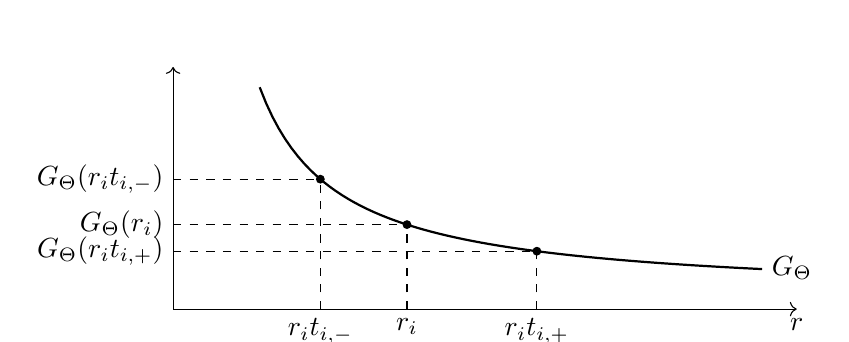
\begin{tikzpicture}[x=1.1cm,y=0.75cm]
\draw[->] (0,0) -- (7.2,0) node[below] {$r$};
\draw[->] (0,0) -- (0,4.1);
\draw[thick,domain=1.0:6.8,samples=80] plot (\x,{3.2/(\x-0.1)+0.2});
\node[right] at (6.8,0.69) {$\tracetwopoint$};
\foreach \xx/\yy/\lab/\vlab in {1.7/2.2/{r_it_{i,-}}/{\tracetwopoint(r_it_{i,-})},2.7/1.4308/{r_i}/{\tracetwopoint(r_i)},4.2/0.9805/{r_it_{i,+}}/{\tracetwopoint(r_it_{i,+})}}{
  \draw[dashed] (\xx,0) node[below] {$\lab$} -- (\xx,\yy);
  \draw[dashed] (0,\yy) node[left] {$\vlab$} -- (\xx,\yy);
  \fill (\xx,\yy) circle (1.6pt);
}
\end{tikzpicture}
\caption{The squeeze. Only $\tracetwopoint$ is monotone (Lemma~\ref{lem:I1.2}). For lattice-rounded separations $t_{i,\pm}\to t_\pm$, $t_-<1<t_+$, the outer values, times $r_i^8\log^2(1/r_i)$, tend to $\traceamplitude t_\pm^{-8}$ along the radii of Lemma~\ref{lem:I-radii}; letting $t_\pm\to1$ gives the limit $\traceamplitude$. Every null sequence has such a subsequence.}\label{fig:I-squeeze}
\end{figure}

\begin{proof}[Proof of Theorem~\ref{prop:TR}]
The phase-table reflection identity E2 of Definition~\ref{def:E1-E3} and the reality of $T$ in Lemma~\ref{lem:G3.2} make $e_{\rm tr}$ real. Lemmas~\ref{lem:G3.1}, \ref{lem:G3.2} and~\ref{lem:H2.4} show that $\Theta$ is real and $O(4)$ invariant and that its continued label is Hermitian and Lorentz scalar. Lemma~\ref{lem:I1.1} gives vacuum centering. For the asymptotic, take any prescribed positive null sequence and the subsequence in~\eqref{eq:I-adjustable}. By Proposition~\ref{prop:I-coefficient}, the phase comparison, and the free normalization in Lemma~\ref{lem:G1.1}, every generic pair $x=(x_0,x_1)$ with $|x|<100$ and $\operatorname{sep}_\infty(x)>1/100$, with $x^{(i)}\in r_i^{-1}a_{n_i}\Z^4$ nearest to $x$, satisfies
\begin{equation*}
r_i^8\log^2(1/r_i)\tracetwopoint(r_i|x_0^{(i)}-x_1^{(i)}|)
\longrightarrow\frac{\traceamplitude}{|x_0-x_1|^8}\,.
\end{equation*}
Translation and $O(4)$ invariance (Lemma~\ref{lem:H1.3}) give $S_2^{\xi_*}(\Theta,\Theta;rx_0,rx_1)=\tracetwopoint(r|x_0-x_1|)$. Here $\slope^{-2}(4d_2)^2=1$, so the amplitude does not depend on~$\slope$.

Take $x_0=0$ and $x_1=(t/2,t/2,t/2,t/2)$, with $1/2<t<2$. This pair is generic and has distance $t$. Monotonicity from Lemma~\ref{lem:I1.2} bounds the lower limit at radius $r_i$ by $\traceamplitude/t^8$ for $t>1$, and the upper limit by that expression for $t<1$ (Figure~\ref{fig:I-squeeze}). Let $t\to1$. The limit along this subsequence is $\traceamplitude$. The subsequence criterion gives the full-radius limit. Here $\traceamplitude=3\dimG/\pi^4>0$ since $\dimG\ge1$; identifying it uses $d_2=-\slope/4\ne0$. Thus $\Theta\ne0$.
\end{proof}

The following high-energy law follows from Theorem~\ref{prop:TR} and Lemma~\ref{lem:I1.2}, as proved below.
\begin{lemma}[High-energy trace limit]\label{lem:I1.3}
For every $\varphi\in C_c(\R^4;\C)\cup\mathcal S$,
\begin{equation*}
\lim_{R_{\rm E}\to\infty}R_{\rm E}^{-8}(\log R_{\rm E})^2\int\varphi(\mathbf p/R_{\rm E})\,d\tracespectrum(\mathbf p)
=\frac{\traceamplitude}{1536\pi}\int_{\forwardcone}\minksquare(\mathbf p)^2\varphi(\mathbf p)\,d^4\mathbf p\,.
\end{equation*}
\end{lemma}
\begin{proof}
The rescaled spectral measures are controlled through their Laplace transforms, which the trace law determines (Definition~\ref{def:D16}, Lemma~\ref{lem:I1.2}). Put $\nu_{R_{\rm E}}=R_{\rm E}^{-8}\log^2R_{\rm E}\,\tracespectrum(R_{\rm E}\,\cdot)$. For every future timelike Laplace covector $u$, with the Euclidean pairing $u\cdot\mathbf p$ of item~\ref{def:W0} of Definition~\ref{def:wightman}, which is the Minkowski pairing of $\mathbf p$ with the future timelike $(-u^1,-u^2,-u^3,u^4)$, Lorentz invariance reduces its transform to the time-axis transform at $s=\sqrt{\minksquare(u)}$. Hence
\begin{equation*}
\int e^{-u\cdot\mathbf p}\,d\nu_{R_{\rm E}}
=R_{\rm E}^{-8}\log^2R_{\rm E}\,\tracetwopoint(s/R_{\rm E})
\longrightarrow \traceamplitude s^{-8}\,.
\end{equation*}
To identify the constant, write $t=\mathbf p^4$ and integrate the spatial radius $q$:
\begin{equation*}
\int_{\forwardcone}e^{-st}\minksquare(\mathbf p)^2\,d^4\mathbf p
=4\pi\int_0^\infty e^{-st}\int_0^t q^2(t^2-q^2)^2\,dq\,dt
=1536\pi s^{-8}\,.
\end{equation*}

The $s=1$ transform bounds compact masses, so diagonal extraction and Riesz representation~\cite[Theorem~2.14]{Rudin1987} give vague subsequential limits. The $u/2$ transform controls the $u$-damped tail, so every limit has the displayed transforms. Holomorphic uniqueness in each coordinate for timelike real part, then Fourier inversion on product Schwartz tests against the finite damped measures~\cite[Theorems~10.18 and~9.11]{Rudin1987}, identify every limit with the cone density in the statement.

For Schwartz tests positivity gives
\begin{equation*}
\nu_{R_{\rm E}}\{\mathbf p^4\le R\}\le e\,R_{\rm E}^{-8}\log^2R_{\rm E}\,\tracetwopoint((R_{\rm E} R)^{-1})\le CR^8
\qquad(R\ge1,\ R_{\rm E}\ge R_{{\rm E},0})\,.
\end{equation*}
Use the trace law at $1/(R_{\rm E}R)$ and $\log R_{\rm E}\le\log(R_{\rm E}R)$. A Schwartz bound of order greater than eight sums the dyadic energy tails uniformly, since $|\mathbf p|\le\sqrt2\mathbf p^4$ on the cone. The $C_c$ limit then gives the Schwartz limit.
\end{proof}

For $\psi_{R_{\rm E}}(x,y)=R_{\rm E}^8\psi(R_{\rm E}x,R_{\rm E}y)$, $\wavetransform\psi_{R_{\rm E}}(\mathbf p)=\wavetransform\psi(\mathbf p/R_{\rm E})$. For $\psi\in\mathcal S_2$, $\wavetransform\psi\in\mathcal S$. Substitution in Lemma~\ref{lem:I1.3} gives the position-space consequence
\begin{equation*}
R_{\rm E}^{-8}\log^2R_{\rm E}\,W_2^{\xi_*}(\Theta,\Theta;\psi_{R_{\rm E}})
\longrightarrow\frac{\traceamplitude}{1536\pi}\int_{\forwardcone}\minksquare(\mathbf p)^2\wavetransform\psi(\mathbf p)\,d^4\mathbf p\,.
\end{equation*}

\subsection{Precise non-free comparisons}\label{sec:partII-I.2}

A finite Wick profile of Definition~\ref{def:D17} is, at small distance, a finite sum of terms $r^a\log^kr$ with $a\in\Z$ and $k\ge0$, plus a bounded remainder; the trace law requires the negative logarithmic power $\log^{-2}(1/r)$. This gives the following exclusion; its proof follows.
\begin{lemma}[Finite Wick obstruction]\label{lem:I2.1}
For every finite Wick profile $W_{\rm Wick}$ and every $\delta>0$, there is $r\in(0,\delta)$ such that
\begin{equation*}
\tracetwopoint(r)\ne W_{\rm Wick}(r)\,.
\end{equation*}
\end{lemma}
\begin{proof}
We expand each profile at small~$r$ and compare with the positive limit of Theorem~\ref{prop:TR}. For one factor, polar coordinates and $\omega_{m_{\rm sh}}=\sqrt{m_{\rm sh}^2+q^2}$ give
\begin{equation*}
K_{m_{\rm sh},k_E,h_{\rm mom}}(r)
=\frac12\left(\int_{S^2}h_{\rm mom}\right)
\int_{m_{\rm sh}}^\infty \omega_{m_{\rm sh}}^{k_E}(\omega_{m_{\rm sh}}^2-m_{\rm sh}^2)^{(j_h+1)/2}e^{-r\omega_{m_{\rm sh}}}\,d\omega_{m_{\rm sh}}\,.
\end{equation*}
For $m_{\rm sh}=0$ this is proportional to $r^{-j_h-k_E-2}$. Otherwise split at $2m_{\rm sh}$; the bounded interval is analytic. On the tail expand $(1-m_{\rm sh}^2/\omega_{m_{\rm sh}}^2)^{(j_h+1)/2}$. Taking enough terms makes the remainder integrable with any prescribed number of energy moments, hence gives a Taylor remainder of the required order. The retained terms are $I_a(r)=\int_{2m_{\rm sh}}^\infty v^ae^{-rv}\,dv$, $a\in\Z$. Integrate explicitly for $a\ge0$; $I_{-1}'=-e^{-2m_{\rm sh}r}/r$ gives the logarithm, and $I_a'=-I_{a+1}$ gives all lower powers. Only nonnegative logarithmic powers occur. For products, choose each remainder order above the other factors' pole orders.

Thus $\operatorname{Re}W_{\rm Wick}=\sum_{a,k}c_{a,k}r^a\log^kr+O(1)$ with finitely many terms. After multiplying by $r^8\log^2(1/r)$, the terms with $a>-8$ vanish. Among the others, the least $a$, then largest $k$, gives a nonzero divergent leading term. A finite limit is therefore zero. Lemma~\ref{lem:I1.2} makes $\tracetwopoint$ real, so equality with $W_{\rm Wick}$ implies equality with its real part. The positive trace limit contradicts equality on $(0,\delta)$, proving also Proposition~\ref{prop:NF}.
\end{proof}

To describe polynomial mass-shell Wick contractions, put $q_m(\mathbf k)=(\mathbf k,\sqrt{m^2+|\mathbf k|^2})$, $m\ge0$. Fix a finite set of elementary field indices, with elements $\mathsf x,\mathsf x'$; words $u,u'$ list its elements. For words of length $k$, $\pi$ ranges over permutations of $\{1,\ldots,k\}$. Comparison data specify finite mass--polynomial lists $\mathcal M_{\rm pair}(\mathsf x,\mathsf x')$, with $P\in\C[\mathbf p^1,\ldots,\mathbf p^4]$, and complex contraction coefficients $c(u,u',\pi)$.
\begin{definition}[Polynomial mass-shell pairings]\label{def:D28}
Set
\begin{equation*}
v_{m,P}(\mathbf k)=\frac{P(q_m(\mathbf k))}{2\omega_m(\mathbf k)},\qquad
L_{m,P}(\varphi)=\int v_{m,P}(\mathbf k)\varphi(q_m(\mathbf k))\,d^3\mathbf k\,.
\end{equation*}
For words $u=(\mathsf x_i)_{i=1}^k$, $u'=(\mathsf x'_i)_{i=1}^k$, define the convolutions of the functionals $L_{m,P}$ by
\begin{equation*}
\mathsf P(u,u';\varphi)=\sum_\pi c(u,u',\pi)
\sum_{(m_i,P_i)\in\prod_i\mathcal M_{\rm pair}(\mathsf x_i,\mathsf x'_{\pi(i)})}
\int\prod_i v_{m_i,P_i}(\mathbf k_i)\,
\varphi\left(\sum_iq_{m_i}(\mathbf k_i)\right)\prod_i d^3\mathbf k_i\,.
\end{equation*}
For unequal lengths put $\mathsf P=0$. A zero denominator at zero momentum gives value zero.
\end{definition}
For finite polynomial fields $Q=\sum_i\alpha_i u_i$, including empty words, the bilinear pairing is $W^{\rm pol}(Q,Q';\varphi)=\sum_{i,j}\alpha_i\alpha'_j\mathsf P(u_i,u'_j;\varphi)$. Empty contractions evaluate $\varphi$ at zero. The shell measure has no $(2\pi)^{-3}$ factor.

The next lemma separates each comparison by one product test; its proof follows.
\begin{lemma}[Polynomial countertest]\label{lem:I2.2}
For every comparison data and every $Q,Q'$, there are $f,h\in\mathcal S$ with compactly supported $\wavetransform(\bar f\otimes h)$ such that
\begin{equation*}
\langle\Phi_\Theta(f)\Omega,\Phi_\Theta(h)\Omega\rangle
\ne W^{\rm pol}(Q,Q';\wavetransform(\bar f\otimes h))\,.
\end{equation*}
\end{lemma}
\begin{proof}
Equality for all product tests would identify the two spectral representations, hence $\tracetwopoint$ with a finite Wick profile, which Lemma~\ref{lem:I2.1} excludes. In detail, equality for all product tests implies equality for every $\varphi\in C_c^\infty$: choose $\widehat h_+=\varphi$ and real $\widehat f_+=1$ on its support. Approximate $e^{-r\mathbf p^4}$ by compact cutoffs. Dominated convergence applies: Lemma~\ref{lem:I1.2} controls $\tracespectrum$; exponential damping controls comparison polynomials at infinity, and $d^3\mathbf k/|\mathbf k|$ is integrable at zero. Expanding the numerators into monomials factors the integrals into the kernels of Definition~\ref{def:D17}, with the empty words giving constants. Hence $\tracetwopoint(r)=W_{\rm Wick}(r)$ for all $r>0$, contrary to Lemma~\ref{lem:I2.1}.
\end{proof}

For the photon comparison use Hilbert tensor products.
\begin{definition}[Ambient and physical Maxwell Fock spaces]\label{def:D29}
For $n\in\N$ colours put
\begin{gather*}
d\sigma(\mathbf k)=\frac{d^3\mathbf k}{2|\mathbf k|},\qquad
\Pi_{ab}(\mathbf k)=\delta_{ab}-\frac{\mathbf k_a\mathbf k_b}{|\mathbf k|^2},\\
\mathcal K_n=L^2(d\sigma;\C^n\otimes\C^3),\qquad
\mathcal F_n=\bigoplus_{k\ge0}\mathcal K_n^{\otimes k},\qquad
\mathcal F_n^{\rm phys}=\bigoplus_{k\ge0}\operatorname{Sym}^k(\Pi\mathcal K_n)\,.
\end{gather*}
The measure has no atom at zero momentum, so the value of $\Pi$ there is immaterial, and $\Pi$ acts pointwise almost everywhere. Thus a physical vector is symmetric and transverse in each slot. Translations multiply sector $k$ by $\exp\{iz\cdot\sum_j(\mathbf k_j,|\mathbf k_j|)\}$. The sector-zero unit is $\Omega_0$.
\end{definition}
\begin{definition}[Coherent comparison vectors]\label{def:D30}
For Schwartz tests $h=(h_{\alpha,a})$, put
\begin{equation*}
v_h(\alpha,a;\mathbf k)=|\mathbf k|\sum_b\Pi_{ab}(\mathbf k)\widehat h_{\alpha,b,+}(\mathbf k,|\mathbf k|),\qquad
\mathcal E(h)=e^{-\|v_h\|^2/2}\bigoplus_{k\ge0}\frac{v_h^{\otimes k}}{\sqrt{k!}}\,.
\end{equation*}
A comparison $U:\mathcal H\to\mathcal F_n$ is a complex linear isometry with image in~$\mathcal F_n^{\rm phys}$, $U\Omega=\Omega_0$, intertwining translations. Set $\psi_U(f)=U\Phi_\Theta(f)\Omega$.
\end{definition}
Real tests have real components. Causal separation means $\minksquare(x-y)<0$ for every pair of points in their closed supports, where $\minksquare(x)=(x^4)^2-\sum_{a=1}^3(x^a)^2$.

Lemma~\ref{lem:I2.2} compares two-point functions only. The Fock test asks more: an embedding of the interacting states into photon Fock space under which the trace field is local relative to the free Maxwell field. Relative locality would impose the equality excluded below. Formally, let $W(h)$ be Weyl operators of the free Maxwell field with $W(h)\Omega_0=\mathcal E(h)$ and $W(h)^*=W(-h)$. If $U\Phi_\Theta(f)U^*$ commuted with $W(h)$ for $h$ causally separated from $f$, then, since $U^*\Omega_0=\Omega$ and $\iota_4\Theta$ is Hermitian,
\begin{align*}
\langle\mathcal E(-h),\psi_U(f)\rangle
&=\langle\Omega_0,W(h)U\Phi_\Theta(f)U^*\Omega_0\rangle\\
&=\langle\Omega_0,U\Phi_\Theta(f)U^*W(h)\Omega_0\rangle
=\langle\psi_U(\bar f),\mathcal E(h)\rangle\,.
\end{align*}
Weyl operators enter only this motivation. The lemma compares the two matrix elements directly, and its proof uses spectral growth without restricting particle amplitudes.
\begin{lemma}[Fock countertest]\label{lem:I2.3}
For every $n\ge0$ and every comparison $U$, for every ball about zero there are Schwartz $f$ compactly supported in that ball and real compactly supported Schwartz $h_{\alpha,a}$, each causally separated from $f$, such that
\begin{equation*}
\langle\mathcal E(-h),\psi_U(f)\rangle
\ne\langle\psi_U(\bar f),\mathcal E(h)\rangle\,.
\end{equation*}
\end{lemma}
\begin{proof}
The proof combines the spectral representation (Lemma~\ref{lem:I1.2}), the high-energy law (Lemma~\ref{lem:I1.3}) and translation covariance (Lemma~\ref{lem:H2.1}) with the dilation behaviour of local photon amplitudes. Fix a ball and suppose equality always holds.

\emph{Sector amplitudes.} Set $p_j=(\mathbf k_j,|\mathbf k_j|)$ and $p_{\rm tot}=\sum_jp_j$. The convolution argument of Lemma~\ref{lem:I1.2} gives sector amplitudes $Y_{k,s}$, with $s$ listing colour and spatial indices:
\begin{equation}\label{eq:I-sector}
\psi_U(f)_{k,s}=\widehat f_+(p_{\rm tot})Y_{k,s},\qquad
\tracespectrum=(p_{\rm tot})_*\sum_{k,s}|Y_{k,s}|^2d\sigma^{\otimes k}\,.
\end{equation}
Box masses are finite. Cauchy--Schwarz and polynomial spectral growth give integrability against sufficiently high inverse polynomials in each momentum.

The common sector unitary $i^k$ preserves the equality, physical vectors and translations. Write $\mathsf Y=i^kY_{k,s}$.

\emph{Locality and doubling.} Expand the coherent equality in a real parameter multiplying $h$, justified by Cauchy--Schwarz and the exponential series. Polarization and complexification give independent complex slot tests. Transversality removes the projector in contractions with physical waves. Shrink nonnegative unit-integral $f$ to zero. Then $|\widehat f_+|\le1$ and $\widehat f_+\to1$; dominated convergence gives, for $g_j$ supported spacelike to zero,
\begin{equation}\label{eq:I-remote}
\int \mathsf Y(\boldsymbol k)\prod_j\big[|\mathbf k_j|\widehat g_{j,-}(p_j)\big]\,d\sigma^{\otimes k}
=\int\overline{\mathsf Y(\boldsymbol k)}\prod_j\big[|\mathbf k_j|\widehat g_{j,+}(p_j)\big]\,d\sigma^{\otimes k}\,.
\end{equation}
Here $\widehat g_-(p)=\widehat g_+(-p)$; the sector factors $i^k$ give exactly these signs.

Fix other slots and use $g(x,t)=a(x)\eta_\epsilon^{(b)}(t)$, with $\eta_\epsilon$ approximating unit mass and $b=0,1$. If $0\notin\operatorname{supp}a$, these are spacelike for small $\epsilon$. Thus both Cauchy data of~\eqref{eq:I-remote} are supported at zero. Weighted integrability bounds their order by $J$, independently of the other tests.

Each datum depends only on the $J$-jet: multiplication by a cutoff in $B(0,\epsilon)$ leaves the distribution unchanged. For a zero-$J$-jet test, Taylor's formula bounds derivatives through order $J$ by $O(\epsilon)$; let $\epsilon\downarrow0$.

The next paragraph proves a uniqueness implication: a combination of sector amplitudes whose two Cauchy data vanish is zero almost everywhere. It is applied below to a polynomial in the doubling operator applied to~$\mathsf Y$, not to~$\mathsf Y$ itself. The massless wave equation separates the frequency branches from these two Cauchy data away from zero momentum. After smearing other slots, each branch is integrable, bounded and holomorphic in its timelike tube, with continuous real boundary. For such a combination with zero Cauchy data, vanishing persists under small translations of the other spacelike tests. Schwarz reflection and holomorphic uniqueness~\cite[Theorems~11.14 and~10.18]{Rudin1987} make the zero set invariant under adding $\R u$ for every future timelike $u$. These vectors span $\R^4$, giving vanishing at every real translation. Successive Fourier inversion~\cite[Theorem~9.11]{Rudin1987} of the smeared integrable amplitudes gives zero almost everywhere. Countably many shrinking bumps remove the other tests: their transforms are eventually nonzero at each momentum.

Let $D_j\mathsf Y(\boldsymbol k)=\mathsf Y(\mathbf k_1,\ldots,2\mathbf k_j,\ldots,\mathbf k_k)$. In the time-order-$b$ Cauchy datum ($b=0,1$), this substitution gives $2^{-3-b}$ times the datum at $a(x)\mapsto8a(2x)$, from $d\sigma(2\mathbf k)=4d\sigma(\mathbf k)$ and $|\mathbf k|^{1+b}$. Spatial jets of order $l$ scale by $2^{3+l}$, giving eigenvalues $2^{l-b}$. Choose a polynomial that annihilates this finite-dimensional dilation action on both Cauchy jets. The uniqueness implication then makes the same polynomial in~$D_j$ annihilate~$\mathsf Y$: for some $J'$,
\begin{equation}\label{eq:I-doubling}
\prod_{a=0}^{J'-1}(D_j-2^{a-1})\mathsf Y=0\qquad\text{in every slot }j\,.
\end{equation}

\emph{Growth.} For $R=2^l$ let $M_{\mathsf Y}(R)=\int_{|\mathbf k_j|\le R}|\mathsf Y|^2d\sigma^{\otimes k}$. By~\eqref{eq:I-sector} and the trace law,
\begin{equation}\label{eq:I-small-mass}
M_{\mathsf Y}(2^l)\le\tracespectrum\{\mathbf p^4\le(k+1)2^l\},\qquad 2^{-8l}M_{\mathsf Y}(2^l)\longrightarrow0\,.
\end{equation}
For the limit, bound the energy mass by $e\,\tracetwopoint(((k+1)2^l)^{-1})$.

Lagrange interpolation in the commuting $D_j$ splits $\mathsf Y$ into joint eigencomponents $D_j\mathsf Y_{\boldsymbol e}=2^{e_j-1}\mathsf Y_{\boldsymbol e}$. Each is a finite combination of doubled copies, so retains~\eqref{eq:I-small-mass}. Moreover $M_{\mathsf Y_{\boldsymbol e}}(2^l)=2^{2l\sum_j e_j}M_{\mathsf Y_{\boldsymbol e}}(1)$, since $d\sigma(2\mathbf k)=4d\sigma(\mathbf k)$.
If $e_j=0$, contraction preserves box mass, contradicting local square integrability and absence of an atom at zero unless the component vanishes. Equation~\eqref{eq:I-small-mass} excludes $\sum_je_j\ge4$. Thus $e_j\ge1$, $\sum_je_j\le3$, and $k\le3$, with box mass $\le CR^6$ for dyadic $R\ge1$. The vacuum sector vanishes by Lemma~\ref{lem:I1.1} and $U\Omega=\Omega_0$.

Summing~\eqref{eq:I-sector} gives $\tracespectrum\{\mathbf p^4\le R\}\le CR^6$ at dyadic $R\ge1$. Multiplication by $R^{-8}\log^2R$ gives zero in the limit, contradicting Lemma~\ref{lem:I1.3} on a nonnegative compact test in $\{0<\mathbf p^4<1,\ \minksquare(\mathbf p)>0\}$.
\end{proof}

An averaged form of this countertest, in which the coherent vectors are moved by maps that preserve physical inner products and fix the image of~$U$, is Lemma~\ref{lem:I2.4} in Section~\ref{sec:correspondence}.

\section{Products and contact subtractions}\label{sec:partII-J}

This section proves Theorems~\ref{prop:OP} and~\ref{prop:CT}. The coefficients of the product expansion are read off by probes. A finite family of probe correlations distinguishes the fields of a fixed degree: two fields of~$F_j$ with the same correlations against every probe are equal. Applied to a cluster of insertions, the probes return finitely many numbers, and a fixed linear reconstruction map, a decoder, returns a field of~$F_j$; on the probe values of a single field it returns that field. Lower degrees are removed before the next degree is read. The probes are chosen once, before the spectators and the phase, and the coefficients are computed from the mixed table; hence they depend on the cluster alone. The remainder is bounded in the commutative compression algebra~$\mathfrak A_0$ of Lemma~\ref{lem:H1.2} before a character is evaluated, and a norm bound in~$\mathfrak A_0$ bounds every character and the mixed vacuum. The coefficients do depend on the prescription, that is, on the table and the probes chosen here; Theorem~\ref{prop:OP} concerns this one coefficient system.

For two fields $A,B$ of degrees $d_A,d_B$ at $x$ and~$0$, with center~$0$ and $|x|\asymp r$, the expansion tested against spectators reads
\begin{equation*}
S^\zeta\bigl(A(x),B(0),\boldsymbol B(y)\bigr)
=\sum_{j\le D}\sum_{\lambda\in\channels{j}}c_{j,\lambda}(A,B;(x,0),0)\,
S^\zeta\bigl(O_{j,\lambda}(0),\boldsymbol B(y)\bigr)+\mathcal R_D^\zeta,
\end{equation*}
with $|c_{j,\lambda}|\le r^{j-d_A-d_B-\varepsilon}$ and $|\mathcal R_D^\zeta|\le r^{D+1-d_A-d_B-\varepsilon}$ for small~$r$; $O_{0,\lambda}$ is a nonzero multiple of the unit. For $D+1<d_A+d_B$ the remainder bound still permits growth as $r\to0$; what increases with~$D$ is its order, and once $D\ge d_A+d_B$ (with $\varepsilon<1$) the remainder tends to zero. Nothing is asserted about a series in~$D$. The expansion goes back to Wilson~\cite{Wilson1969}; Fr\"ob and Holland prove its existence for Euclidean Yang--Mills theory to all orders in perturbation theory~\cite{FrobHolland2016}. The expansion here is nonperturbative, at each finite truncation, with one coefficient system for every phase.

The lattice estimate starts from the signed local and graded quotient bounds of Lemmas~\ref{lem:J-signed-local} and~\ref{lem:J-graded-quotient}. Each insertion carries a nilpotent external field with a weight. Blocking loses mark weight when insertion points approach one another; grouping nearby markers bounds this loss by a power of the ratio of insertion and fusion scales (Figure~\ref{fig:J-scales}). Taylor subtraction and transport of the coefficient back to a coarser level produce one field and a small remainder, whose chessboard seminorm reflection positivity converts into a norm bound in~$\mathfrak A_0$. Derivative induction removes the restriction to grid points; tree induction allows several clusters to shrink at independent rates. The nested and integrated forms (Lemmas~\ref{lem:J1.4}--\ref{lem:J1.5} and Remark~\ref{lem:J1.3}) are not used in the proofs of Theorems~\ref{thm:A} and~\ref{thm:B}. The contact extension of Section~\ref{sec:partII-J.2} is defined from the continuum correlations at distinct points, not as a lattice limit at coincident points; the lattice bounds of Lemma~\ref{lem:J-power-separated} make its shell sums converge.

Throughout, the lattice insertions and quotient fields are those of Definitions~\ref{def:D08} and~\ref{def:D10}; inclusions and derivatives are those of Lemma~\ref{lem:F2}. The rotations~$R_j(h)$ are those of Lemma~\ref{lem:G3.1}. Write $|\boldsymbol A|_{\deg}=\sum_i\deg A_i$ and $\zeta\in\phases\sqcup\{\mathrm{mix}\}$, as in Definition~\ref{def:D18}.

\paragraph{Inputs from the marked expansion and the quotient.}

The lattice replacement and its continuum consequences below use the full marked-source propagation of Lemma~\ref{lem:E-source-attachments}, including the stronger anchored higher-mode estimate and the stopping-level restart at support exponent~$98$ not yet established there. The quotient and operator bounds also use the same-sample guarded comparison and actual graph-operator continuity identified in Section~\ref{sec:partII-F}. Thus Lemmas~\ref{lem:J-lattice} and~\ref{lem:J-power-separated}, and the OPE and contact conclusions derived from them, are conditional on those inputs for the selected family.

We first establish two estimates needed when the field to be extracted varies with the cutoff. Throughout this subsection, a local marked expression has the form of Definition~\ref{def:D26} and the regularity, zero radial jets and forced supports of Lemma~\ref{lem:E2.2a}. Write
\begin{equation*}
\mu(x)=\sum_\alpha|x_\alpha|,\qquad x^\circ=x-x_0\mathbf1,
\qquad \mathfrak r_i=\mathcal E_i+(\epsilon_i^{\rm for})^{-1/2}\mathcal K_i\,.
\end{equation*}
The last quantity is the weighted remainder mass of Lemma~\ref{lem:E2.2}. Fix an output degree~$t$. The diagonal rescaling $(\mathsf d_i x)_\alpha=\ell_i^{t-\deg\alpha}x_\alpha$ accounts for the engineering degrees inside~$V_t$. Write $C_i=C^{\rm col}_{J_i}$ for the column bound at level~$i$. A normalized column at level~$i$ is the local expression~$\mathfrak c_i(b)$ of Lemma~\ref{lem:E2.1} with coefficient vector~$b$; its coefficient map is~$\mathsf C_i$, and its remainder bound is $C_i\mu((\mathsf C_i b)^\circ)$ by Lemma~\ref{lem:E2.2}.

Let $K_j\ge1$ be the nondecreasing stage bound fixed before item~\ref{it:E-columns} of Section~\ref{sec:partII-E.1}. The degree rescaling above is the map $\mathsf S_L$ in the proof of Lemma~\ref{lem:E-marked-step}. For an input coefficient~$v$ and remainder mass~$q$, its averaged marked estimate gives an output coefficient~$u$ and remainder mass~$r$ with
\begin{equation}\label{eq:J-marked-recall}
\begin{aligned}
\mu(u-M_i\mathsf d_iv)&\le\epsilon_i[\mu(v^\circ)+q],\\
r&\le K_{J_{i+1}}\mu((\mathsf d_iv)^\circ)+\epsilon_iq,\qquad\epsilon_i=\ell_i^{-3/8}.
\end{aligned}
\end{equation}
Here $M_i$ is the leading polynomial map, fixes the unit, preserves the nonconstant subspace, and satisfies $\|M_i^{\pm1}\|\le K_{J_{i+1}}$. These estimates follow from~\eqref{eq:E-atom-estimates} and the symmetry averaging in that proof. In the threshold order of Section~\ref{sec:constants}, the construction chooses
\begin{equation}\label{eq:J-stage-room}
\begin{aligned}
64K_{J_l+1}^2&\le C_l,&
10^5K_{J_{l+1}+1}^6(1+C_{l+1})^2&\le\ell_l^{1/8},&
1+2C_l&\le\ell_l^{1/40}.
\end{aligned}
\end{equation}
The column choice imposes the first inequality; the ratio choice imposes the other two. Stage growth gives $J_{l+1}\le J_l+1$.

The next estimate retains the signed difference produced by subtracting a column. A transported family on~$[k_*,m]$ is a sequence of local marked expressions $\mathfrak c_l(b_l)+R_l$, $k_*\le l\le m$, in which $R_l$ has coefficient zero and each term arises from the next finer one by one marked integration step of Lemma~\ref{lem:E-marked-step}. Its measured coefficient is $x_l=\mathsf C_l b_l$, and $r_l$ is its remainder bound. Its free affine parameter is a vector added to the column input at the finest level~$m$. Write $q_{\rm fin}$ for the combined coefficient and remainder bound of the original expression at~$m$, before this affine subtraction. In the next lemma, the interval~$[k_*,m]$ is sufficiently late.

\begin{lemma}[Signed local transport]\label{lem:J-signed-local}
(a) Every normalized column plus a zero-coefficient remainder at level~$m$ admits a transported family on~$[k_*,m]$. Its densities satisfy $H_l=\ell_l^t\blockmap{l}_{\beta_{N,p,l+1}}H_{l+1}$ $(k_*\le l<m)$, each step satisfies~\eqref{eq:J-marked-recall}, $r_m\le(1+C_m)q_{\rm fin}+C_m\mu(x_m)$, and the free affine parameter can be chosen so that $x_{k_*}=0$.

(b) If $x_{k_*}=0$, then, for $k_*\le l\le m$,
\begin{equation*}
r_l+\mu(x_l)\le4(1+C_m)q_{\rm fin}(a_m/a_l)^{1/8},\qquad
r_m\le2(1+C_m)q_{\rm fin}\,.
\end{equation*}
\end{lemma}
Thus a residual that starts with zero coefficient at the coarse end loses only the factor $4(1+C_m)$ at the fine end, and gains $(a_m/a_l)^{1/8}$ at every coarser level.

\begin{proof}\label{proof:J-signed-start}
The termwise remainder estimates and the Lipschitz bound in the proof of Lemma~\ref{lem:E-marked-step} control one step; the exact column identity of Lemma~\ref{lem:E2.1} keeps the densities exact; an induction along the interval turns the signed one-step inequalities into the discount.

Let~$R$ have coefficient zero and remainder bound~$q_0$. Its regular terms have zero radial jets through~$t$, by the local format of Lemma~\ref{lem:E2.2a}; its forced terms retain their eligibility events. In the marked integration of Lemma~\ref{lem:E-marked-step}, the former gain an inverse block factor before the connected sums, and the latter keep half the forced suppression. The stage constants precede the ratio and its entry threshold, so both resulting bounds $C^{\rm loc}_{J_{i+1}}/\ell_i+o_{\widehat\beta_i}(1)$ are at most~$\ell_i^{-2/5}$. Sum the regular masses~$g_a$ and forced masses $k_b/(\epsilon_{i+1}^{\rm for})^{1/2}$ before taking the output norm. Their sum is at most~$q_0$. The termwise bounds in that proof, or its Lipschitz estimate for the difference between a column plus~$R$ and the same column, therefore bound the output coefficient and remainder by~$\ell_i^{-2/5}q_0$. The rooted clause of Lemma~\ref{lem:D-connected}, in the marked norm defined below, justifies termwise integration and retains the exact density identity. The last inequality of~\eqref{eq:J-stage-room} gives $(1+2C_i)\ell_i^{-2/5}\le\epsilon_i$. If~$Z$ denotes the resulting local expression and~$z$ its coefficient, then
\begin{equation*}
H(Z)=\ell_i^t\blockmap{i}_{\beta_{N,p,i+1}}H(R),\qquad
\mu(z)\le\ell_i^{-2/5}q_0,\qquad\mathfrak r_i(Z)\le\ell_i^{-2/5}q_0\,.
\end{equation*}

Write the fine affine family as $\mathfrak c_{i+1}(a+b)+R$, with~$b$ the free parameter. Set $c=\mathsf C_i^{-1}z$ and replace it at the coarse level by
\begin{equation*}
\mathfrak c_i(a+c+b)+R',\qquad
R'=Z-\mathfrak c_i(c)\,.
\end{equation*}
The coefficient of~$R'$ is zero, and $\mathfrak r_i(R')\le(1+C_i)\ell_i^{-2/5}q_0$.
Linearity of the column density gives
$H(\mathfrak c_i(a+c+b))+H(R')=H(\mathfrak c_i(a+b))+H(Z)$.
Together with the exact column identity of Lemma~\ref{lem:E2.1}, this proves the asserted density identity for every~$b$, including all forced terms. The supports remain fixed in~$b$ by Lemma~\ref{lem:E2.2}.

For the column alone use~\eqref{eq:J-marked-recall}, with fine remainder bound~$q_{\rm col}$. Adding~$Z$ changes the coefficient by at most~$\ell_i^{-2/5}q_0$. For the remainder, recentering costs at most~$C_i\ell_i^{-2/5}q_0$, and shifting the column parameter costs at most another~$C_i\ell_i^{-2/5}q_0$. The total extra cost is $(1+2C_i)\ell_i^{-2/5}q_0\le\epsilon_iq_0$. With~$q=q_{\rm col}+q_0$, these are the asserted bounds. Repeating this construction from the fine end to the chosen coarse end produces the transported family on the whole interval.

For later use put $U=\mu(u)$, $Y=\mu(\mathsf d_iv)$, $K=K_{J_{i+1}}$ and retain~$r,q$ for the remainder bounds. Applying~$M_i^{-1}$ and using $\mu(v^\circ)\le Y$ gives
\begin{equation}\label{eq:J-signed-input}
Y\le K[U+\epsilon_i(Y+q)],\qquad r\le KY+\epsilon_iq\,.
\end{equation}
For an interval~$[k_*,m]$, choose the free affine parameter to cancel the coefficient at~$k_*$; this uses the invertibility of~$\mathsf C_{k_*}$. The signed residual then starts with coefficient zero. In step~$l$ put $K=K_{J_{l+1}}$ and $A_l=32(1+C_l)^2$. Induct from~$k_*$ toward~$m$ on the cone condition $A_l\mu(x_l)\le r_l$, which says that the coefficient is small compared with the remainder bound; it holds at~$k_*$ because $x_{k_*}=0$. Equation~\eqref{eq:J-stage-room} implies
\begin{equation*}
A_l\ge4K^2,\quad4K\epsilon_l\le1,\quad
4KA_{l+1}\epsilon_l\le1,\quad
(4K^2+1)\ell_l^{1/8}\epsilon_l\le1.
\end{equation*}
In~\eqref{eq:J-signed-input} at step~$l$, $U=\mu(x_l)$, $r=r_l$ and $q=r_{l+1}$. From $A_lU\le r\le KY+\epsilon_lq$ and $A_l\ge4K^2$ obtain $4KU\le Y+\epsilon_lq$. Substitution into~\eqref{eq:J-signed-input} gives $Y\le4K\epsilon_lq$. Thus $A_{l+1}\mu(x_{l+1})\le q$, since $\mu(x_{l+1})\le Y$; this is the cone condition at~$l+1$. Also $\ell_l^{1/8}r\le q$. Iteration gives the discount~$(a_m/a_{k_*})^{1/8}$. At the finest level the affine subtraction has $r_m\le(1+C_m)q_{\rm fin}+C_m\mu(x_m)$. The cone condition at~$m$ and $A_m\ge2C_m$ give $2C_m\mu(x_m)\le r_m$, hence $r_m\le2(1+C_m)q_{\rm fin}$ and $r_m+\mu(x_m)\le4(1+C_m)q_{\rm fin}$. Applying the iterated discount between any~$l$ and~$m$ proves the interval bound.
\label{proof:J-signed-end}
\end{proof}

The next estimate recovers the output-degree power after passing to the quotient. Fix any norm on~$F_t$. Put $\|v\|_m=\mu(x_m(v))$, where $x_m(v)=x_{N,p,m;t}(v)$ is the transferred coefficient of Definition~\ref{def:D08}. A refinement below is a nontrivial refinement of the ordered cutoff limits~\eqref{eq:E2-tails}; it may depend on the cluster geometry.

\begin{lemma}[Graded quotient bound]\label{lem:J-graded-quotient}
For $0\le i\le t$ there are positive~$C_{t,i}(m)$, independent of the refinement and label family, with $\log C_{t,i}(m)/s_m\to0$. If labels~$v_{N,p}\in V_t$ converge in~$V_t$ to~$v$ on such a refinement and eventually $\|v_{N,p}\|_m\le\epsilon_{\rm bd}$, then
\begin{equation}\label{eq:J-graded-input}
\operatorname{dist}_{F_t}([v],\jmath_{i-1,t}F_{i-1})
\le C_{t,i}(m)a_m^{-(t-i)}\epsilon_{\rm bd}\,.
\end{equation}
Here $[v]\in F_t$ is the class of~$v$, $F_{-1}=0$, and $m$ is sufficiently large.
\end{lemma}
A label that is small at level~$m$ is therefore, in the quotient and up to subpower factors, within $a_m^{-(t-i)}$ times its size of the fields of degree below~$i$.

\begin{proof}\label{proof:J-graded-start}
The triangularity of the leading map proved in Lemma~\ref{lem:E-marked-step} separates high from low engineering degrees; the marked bounds of Lemma~\ref{lem:E2.2} control the error; the physical quotient of Definition~\ref{def:D10}, with the corrected inclusions of Lemma~\ref{lem:F2}, identifies the removed low-degree part with a lower field. In the notation of~\eqref{eq:J-marked-recall}, the triangularity is
\begin{equation*}
(M_l)_{\alpha\beta}=0\quad
(\alpha\ne\beta,\ \deg\alpha\le\deg\beta).
\end{equation*}
The diagonal entries are the nonzero fine-to-coarse normalization factors. The full coefficient map differs from this leading map by the marked error. Write~$P$ for coordinate projection onto engineering degrees at most~$i-1$, first assuming~$i>0$. The leading map~$M_l$ and its inverse preserve~$\ker P$: triangularity gives preservation by~$M_l$, and injectivity on this finite-dimensional subspace gives preservation by its inverse. Consequently $\mu(Px)\le K_{J_{l+1}}\mu(PM_lx)$.
The degree rescaling expands~$Px$ by at least~$\ell_l^{t-i+1}$, whereas it expands~$x-Px$ by at most~$\ell_l^{t-i}$. The marked error is bounded by $\epsilon_l\mu(x^\circ)$.

The two resulting estimates are
\begin{align*}
\mu(x_{l+1})\le C_{l+1}\mu(Px_{l+1})
&\ \Longrightarrow\
\begin{cases}
\mu(x_l)\le C_l\mu(Px_l),\\
\ell_l^{t-i+1}\mu(Px_{l+1})\le C_{l+1}\mu(Px_l),
\end{cases}\\
Px_{l+1}=0&\ \Longrightarrow\
\mu(x_l)\le C_{l+1}\ell_l^{t-i}\mu(x_{l+1})\,.
\end{align*}
To obtain the first line, put $Y=\mu(P\mathsf d_lx_{l+1})$. The low-cone hypothesis $\mu(x_{l+1})\le C_{l+1}\mu(Px_{l+1})$ and $C_{l+1}\le\ell_l$ give $\mu(\mathsf d_lx_{l+1})\le2Y$. Applying the inverse leading map to the low coordinates and using $2K_{J_{l+1}}\epsilon_l(1+C_{l+1})\le1$ gives $Y\le2K_{J_{l+1}}\mu(Px_l)$. The full coefficient is at most $3K_{J_{l+1}}Y$, so $64K_{J_{l+1}}^2\le C_l,C_{l+1}$ gives both conclusions. In the second line use $\mu(\mathsf d_lx_{l+1})\le\ell_l^{t-i}\mu(x_{l+1})$ and $K_{J_{l+1}}+1\le C_{l+1}$. These numerical inequalities follow from~\eqref{eq:J-stage-room}.

At the bare level take the plane~$PV_t$. Its transported image remains in the low cone by the first line. The map from this plane to its low coordinates at any level is injective by its expansion bound, hence onto~$PV_t$. Subtracting a transported vector with the same low coordinates at level~$m$ therefore leaves zero low coordinates and increases the full size by at most~$1+C_m$. Repeat the subtraction at every next coarser level, applying the second line between subtractions. This gives a vector~$y_{N,p}$ in the transported bare low plane with
\begin{equation*}
\|v_{N,p}-y_{N,p}\|
\le G_m(1+C_m)(a_{\reflevel{t}}/a_m)^{t-i}\epsilon_{\rm bd},
\qquad G_m=\prod_{l<m}(1+C_l)C_{l+1}\,.
\end{equation*}
Allowing a fixed norm-equivalence factor, put $\mathcal J_m=\prod_{l<m}C_{l+1}$. The first-line expansion, iterated from the bare level, shows that bounded vectors~$y_{N,p}$ in this plane have bare coefficients bounded by $a_N^{t-i+1}e^{o(s_N)}$. Multiplying the same polynomial by $a_N^{i-1}$ instead of~$a_N^t$ therefore gives a degree-$(i-1)$ local observable with subpower healthy derivative and all-configuration supremum bounds. Its stencil is unchanged. To match this observable to the selected lower-degree insertions, apply Lemma~\ref{lem:E-local-comparison}(i): it gives tame degree-$(i-1)$ coefficients~$c_{N,p}$ whose insertions differ from these observables by a negligible error (Definition~\ref{def:E2-small}). Lemma~\ref{lem:F1b} removes that error in every separated spectator test.

To pass to a physical lower field, apply Lemma~\ref{lem:F-represent} in~$V_{i-1}$ to the family~$c_{N,p}$, with the equation projections $\Pi_{N,p}=\Pi_{i-1,N,p}$ of Lemma~\ref{lem:E2.6}, taken along $N=\mathsf n(j)$ and $p=P(k)$, their limit~$\Pi_{i-1}$ from~\eqref{eq:F-projections}, and the one-slot spectator functionals, whose kernels intersect in~$\ker\Pi_{i-1}$ by~\eqref{eq:F-dimension}. The normalized equation remainder $(c_{N,p}-\Pi_{N,p}c_{N,p})/(1+\|\Pi_{N,p}c_{N,p}\|)$ is tame, being a bounded multiple of~$c_{N,p}$ minus a family of norm at most one; Lemmas~\ref{lem:E2.7} and~\ref{lem:F1b} make its separated spectator tests tend to zero. If~$y$ is a limit of the bounded labels~$y_{N,p}$, the lemma gives a label in~$V_{i-1}$ with exactly the limiting correlations of~$y$. The corrected inclusions of Lemma~\ref{lem:F2} and the all-spectator definition of the null space now give $[y]\in\jmath_{i-1,t}F_{i-1}$. Boundedness of~$y_{N,p}$ follows from the displayed distance bound and convergence of~$v_{N,p}$. If these bounds hold only on the chosen refinement, set~$y_{N,p}=0$ off the set where they hold; this extends the bounded plane family to the original tails without changing its limit. Passing to this limit proves the distance estimate.

For~$i=0$ no plane is removed. Iterating the reverse coefficient estimate of Lemma~\ref{lem:E2.2} gives $\|v\|\le \mathcal J_m(a_{\reflevel{t}}/a_m)^t\epsilon_{\rm bd}$ and hence the same bound in~$F_t$. Finally $\log \mathcal J_m=o(s_m)$, since $\log C^{\rm col}_{J_{m+1}}\le J_{m+1}^{-2}\log\ell_m$ (Section~\ref{sec:constants}) and by Lemma~\ref{lem:E1.1}. Since $C_l\ge2$, $G_mC_m\le (\mathcal J_m)^3C_0$. Thus $\log G_m=o(s_m)$ as well. Fixed reference-spacing and quotient-norm factors are absorbed in~$C_{t,i}(m)$. No estimate depends on the refinement used to take the limits.
\label{proof:J-graded-end}
\end{proof}


\subsection{Products and nested clusters}\label{sec:partII-J.1}

A probe word is a fixed finite list of fields at distinct nonzero points. Correlating a field at the origin against such a word gives a linear functional on~$F_j$. The intersection of the kernels of all these functionals is zero, by the definition of~$\nullspace{j}$. Finite dimensionality therefore permits a finite separating collection.

Choose the probe functionals recursively. Given biorthogonal fields~$u_\alpha$ and probe functionals~$\ell_\alpha$ below degree~$j$, continue each~$\ell_\alpha$ to~$F_j$ by the same correlation formula; inclusions preserve that formula by Lemma~\ref{lem:F2}. The retraction
\begin{equation*}
\mathsf t_jA=\sum_{\deg\alpha<j}\ell_\alpha(A)\jmath_{\deg\alpha,j-1}u_\alpha,
\qquad\mathsf t_j\jmath_{j-1,j}=1
\end{equation*}
allows a section~$s$ of the new quotient to be replaced by $s-\jmath\mathsf t_js$. Lift a quotient basis with this section and realize its dual by finite combinations of probe functionals, which span~$F_j^*$. The enlarged system is biorthogonal. In particular~$\ell_\alpha$ vanishes on~$\jmath F_{\deg\alpha-1}$. For $j=0$ take $u_0=\mathbf1$. Let~$\mathcal P_j$ be the union of the finite probe sets used through degree~$j$, with index~$\gamma$. Write $\ell_\alpha(A)=\sum_\gamma m_{\alpha\gamma}S(A(0),B_{j,\gamma})$ in this finite collection.

\begin{definition}[Finite correlation projection]\label{def:D31}
Define the linear reconstruction map $D_j:\C^{\mathcal P_j}\to F_j$ by
\begin{equation*}
D_j(y)=\sum_{\deg\alpha\le j}\left(\sum_{\gamma\in\mathcal P_j}m_{\alpha\gamma}y_\gamma\right)\jmath_{\deg\alpha,j}u_\alpha\,.
\end{equation*}
With $\operatorname{ev}_j(A)=(S(A(0),B_{j,\gamma}))_{\gamma\in\mathcal P_j}$, it satisfies $D_j\operatorname{ev}_j=\mathrm{id}_{F_j}$: it is a fixed left inverse of field evaluation.
For a word~$w$ separated from these probes, set
\begin{equation*}
P_j^{\rm raw}w=D_j\big((S(w,B_{j,\gamma}))_{\gamma\in\mathcal P_j}\big)\,.
\end{equation*}
This extracts a field from finitely many correlations using the fixed biorthogonal coordinates.
\end{definition}

Here and below a word is a finite product of labelled insertions; sums of words are read linearly. Rotations act on every position and label, and conjugation acts on labels and scalar coefficients. Translation of a word by~$u$ is denoted by~$\tau_u$.

\begin{definition}[Symmetric projection]\label{def:D32}
When every rotation of~$w$ is separated from every probe in~$\mathcal P_j$, set
\begin{equation*}
A_jw=\int_{O(4)}R_j(h)P_j^{\rm raw}(h^{-1}w)\,dh,\qquad
B_jw=\tfrac12\big(A_jw+\overline{A_j\bar w}\big)\,.
\end{equation*}
The Haar measure has mass one. Outside this domain set both maps to zero. At center~$o$, apply these formulas to~$\tau_{-o}w$. These averages impose rotation covariance and reality.
\end{definition}

Let~$I_qA=A(0)$ for~$A\in F_q$. The inclusions~$\jmath_{i,j}$ identify the same field in different degrees.

\begin{definition}[OPE coefficients]\label{def:D33}
Put $L_{i,q}=B_iI_q$ and define
\begin{equation*}
Q_0=1,\qquad Q_j=1-\sum_{i<j}\jmath_{i,j}Q_iL_{i,j},\qquad
E_j=\bigcap_{i<j}\ker(Q_iL_{i,j})\,.
\end{equation*}
For the chosen real basis~$(O_{j,\lambda})_{\lambda\in\channels{j}}$ of~$E_j$, let~$\omega_{j,\lambda}:E_j\to\C$ be its coordinate functionals and set
\begin{equation*}
c_{j,\lambda}(\boldsymbol A;x,o)
=\omega_{j,\lambda}\!\left(Q_jB_j\!\left[\prod_i A_i(x_i-o)\right]\right)\,.
\end{equation*}
The recursion removes lower degrees before reading coordinates and is independent of arity and truncation.
\end{definition}

In the first two degrees the recursion reads as follows. In degree zero, $Q_0=1$: the degree-zero probes read the multiple of the unit line seen by the cluster. In degree one, $L_{0,1}=B_0I_1$ reads the degree-zero part of a single degree-one field, and
\begin{equation*}
Q_1B_1w=B_1w-\jmath_{0,1}B_0\bigl[(B_1w)(0)\bigr].
\end{equation*}
This is the field read in degree one, minus the multiple of the unit that the degree-zero probes see in it. The degree-one coefficients are the coordinates of this difference in $E_1=\ker L_{0,1}$.

The following splitting makes the coefficients a single choice for all later estimates.

\begin{lemma}[One channel prescription]\label{lem:J1.1}
The real fields~$O_{j,\lambda}$ form complex bases of conjugation-invariant complements:
\begin{equation*}
F_j=\jmath_{j-1,j}F_{j-1}\oplus E_j,\qquad
E_j=\operatorname{span}_{\C}\{O_{j,\lambda}:\lambda\in\channels{j}\},\qquad F_{-1}=0\,.
\end{equation*}
The degree-zero vector spans the unit line and need not equal the unit.
\end{lemma}
By Definition~\ref{def:D33}, all coefficients are fixed before spectators, states and truncations.

\begin{proof}
The biorthogonal construction preceding Definition~\ref{def:D31} gives a reconstruction formula fixing every field of~$F_j$; the field calculus of Lemma~\ref{lem:F2} makes the old functionals compatible with the inclusions. Continuing an old functional means using the same finite correlations, since $\iota_j\jmath_{q,j}=\iota_q$; no extension of a functional is chosen arbitrarily.

For~$i\ge q$, this reconstruction and the rotation and reality laws give~$L_{i,q}=\jmath_{q,i}$. Also $L_{i,j}\jmath_{q,j}=L_{i,q}$ for~$i<q\le j$: both sides evaluate the same single-field word before averaging. For all~$q\le j$, induction in~$j$ now gives
\begin{equation}\label{eq:J-cuts}
Q_jL_{j,q}=0\ (q<j),\qquad
\sum_{i\le j}\jmath_{i,j}Q_iL_{i,q}=\jmath_{q,j}\,.
\end{equation}
For~$q=j$ the second identity is the recursion; for~$q<j$, compose that recursion with~$\jmath_{q,j}$ and use the compatibility just proved and the induction hypothesis. In the same induction assume $Q_kF_k\subset E_k$ and $Q_k=1$ on~$E_k$ for~$k<j$. Applying~$Q_iL_{i,j}$ to~$Q_jA$ then cancels its matching~$i$ term; terms with~$k<i$ vanish because $Q_iL_{i,j}$ vanishes on $\jmath_{i-1,j}F_{i-1}$, and terms with~$i<k<j$ vanish because~$Q_kA\in E_k$. Thus~$Q_jF_j\subset E_j$. On~$E_j$, the defining sum for~$Q_j$ is zero, so~$Q_j=1$. Its kernel is exactly~$\jmath F_{j-1}$ by~\eqref{eq:J-cuts}. Haar invariance and simultaneous input and output conjugation show that every map $Q_iL_{i,j}$ intertwines rotations and conjugation. Thus~$E_j$ is invariant under both. Its fixed real subspace spans it, since $v=(v+\bar v)/2+i(v-\bar v)/(2i)$; a real basis is also a complex basis. This proves the stated splitting and the simultaneous choice.
\end{proof}

For $T\to\infty$ write $f\preccurlyeq e^{bT}$ when, for every~$\tau>0$, there is~$T_0$ such that for every~$T\ge T_0$ an ordered cutoff tail gives $\|f\|\le e^{(b+\tau)T}$, uniformly in the cutoff and volume on that tail. Thus the decaying quantity $e^{-2T}$ has exponent $-2$: its upper bound allows the small loss $e^{\tau T}$. Products add exponents and finite sums take their maximum. Factors of exponent zero are called subpower. A level~$k$ has height~$b$ when~$s_k/T\to b$; thus $a_k=e^{-bT+o(T)}$. Lemma~\ref{lem:E1.1} supplies these levels by taking the first with $s_k\ge bT$, or $s_k\ge\sqrt T$ if~$b=0$.

Insertions are carried through the integration by nilpotent external fields. This is the device used for observables by Bauerschmidt, Brydges and Slade, who add an external observable field to the interaction and truncate the algebra in it~\cite[Section~2.3]{BauerschmidtBrydgesSlade2015}. A marker is one group of insertions in the reflected cells not yet fused with another; it is live while its weight is positive. To each marker~$\iota$ attach a commuting variable $z_\iota$ with $z_\iota^2=0$ and a mark weight~$w_\iota>0$. In this finite scalar algebra put
\begin{equation*}
c=\sum_Ac_Az_A,\qquad z_A=\prod_{\iota\in A}z_\iota,\qquad
\|c\|_{\rm mark}=\sum_A|c_A|\prod_{\iota\in A}w_\iota,
\qquad c_A\in\C\,.
\end{equation*}
Products of monomials with overlapping markers vanish, and the weights of disjoint markers multiply, so $\|cd\|_{\rm mark}\le\|c\|_{\rm mark}\|d\|_{\rm mark}$. The coefficient of~$z_A$ in $\rho\prod_\iota(1+z_\iota O_\iota)$ is $\rho\prod_{\iota\in A}O_\iota$; by linearity, taking this coefficient commutes with integration of integrable terms.

If $F_{X,A}$ is a coefficient with support~$X$ and marker set~$A$, its weighted majorant is
\begin{equation*}
\sum_{X,A}e^{\sigma\cover(X)}\|F_{X,A}\|\prod_{\iota\in A}w_\iota\,.
\end{equation*}
Here $\|F_{X,A}\|$ is the derivative or forced majorant of Definitions~\ref{def:D05a}--\ref{def:D05b}; at a support ball use its anchored sum. The factors $e^{\sigma\cover(X)}\|F_{X,A}\|$ enter as~$v_a$ in Lemma~\ref{lem:D-connected}. Only the marked norm is used submultiplicatively. A grouped coefficient carries the product of its live mark weights, denoted by~$\omega$.

For the marked expansion put
\begin{equation*}
\delta_l^{\rm mark}=\widehat\beta_{l+1}^{-2},\qquad
\phi_l=\widehat\beta_{l+1}^{-1},\qquad
\Xi_l=\exp\sqrt{\widehat\beta_{l+1}},\qquad
y_{t,l}=\widehat\beta_l^{-\nu_t}.
\end{equation*}
The fixed integer~$\nu_t$ bounds the local degree-$t$ polynomial losses, and $y_{t,l}C_l\le1$ at entry. The four factors pay respectively for support enlargement, regular transport, Taylor extraction and insertion normalization. Their logarithms and~$\log C_l$ are $o(s_l)$. For an initial weight~$\varpi>0$ at~$k_*$ define its later weights by
\begin{equation*}
\varpi_{k_*}=\varpi,\qquad \varpi_{l+1}=\phi_l\varpi_l\quad(l\ge k_*).
\end{equation*}
The marked entry choices require $\phi_l\ell_l^{t+1}y_{t,l}\le y_{t,l+1}$ for $l\ge \reflevel{t}$. This follows the zero-jet regular remainder through the integration.

Let $B_l$ be the support radius and $q_l$ the per-site logarithmic bound~\eqref{eq:E-vacuum-majorant} of Section~\ref{sec:constants}. Fix a reflected cell at level~$k$ and choose
\begin{equation*}
k_*=\min\{l\ge k:B_l^2\le a_k/a_l\},\qquad
N_k=\exp\{(a_k/a_{k_*})^4q_{k_*}+5\}.
\end{equation*}
These quantities ensure that the marked stencils fit in the cell and bound its density normalization.

For a grouped coefficient at level~$m+1$ of weight~$\omega>0$, put
\begin{equation*}
q^{\rm ext}_m=4\Xi_ma_{m+1}^t/\omega,\qquad \mathfrak E_m=8(1+C_m)q^{\rm ext}_m\,.
\end{equation*}
The terminal weight~$\varpi$ must satisfy
\begin{equation}\label{eq:J-marked-weights}
\begin{aligned}
\varpi(a_m/a_{k_*})^{t+1}y_{t,m}/y_{t,k_*}
 &\le\delta_m^{\rm mark}\omega/(16\Xi_m),\\
32(1+C_m)\varpi\,a_{k_*}^{-t}\mathfrak E_m(a_m/a_{k_*})^{1/8}
 &\le y_{t,k_*}/2.
\end{aligned}
\end{equation}
These conditions pay for extraction at~$m$ and for the transported residual, respectively.

Informally, after blocking down to level~$m$, a group of insertions of total weight~$\omega$ is replaced by one degree-$t$ insertion at the origin, the matched field. The next lemma bounds its coefficient by~$2\mathfrak E_m$, and the chessboard seminorm of the replacement error in a level-$k$ cell by~$2N_k/\varpi$.

\begin{lemma}[Marked extraction and insertion costs]\label{lem:J-marked-costs}
A grouped coefficient of weight~$\omega$ has a degree-$t$ local extraction with coefficient and remainder each at most~$q^{\rm ext}_m$. With $k_*$ as above, sufficiently late, and whenever~\eqref{eq:J-marked-weights} holds, the matched field has coefficient size at most~$2\mathfrak E_m$. Its interior reflected remainder in the level-$k$ cell has chessboard seminorm at most~$2N_k/\varpi$.
\end{lemma}

\begin{proof}\label{proof:J-costs-start}
The extraction is a Taylor expansion in the norms of Definitions~\ref{def:D05a}--\ref{def:D05b} and~\ref{def:D08}; Lemma~\ref{lem:J-signed-local} transports its residual to~$k_*$; the majorants of Lemma~\ref{lem:D1}, summed by the rooted clause of Lemma~\ref{lem:D-connected} in the marked norm, bound the cell integral. Divide a grouped coefficient by its available weight~$\omega$. Extract its radial polynomial through~$t$ and write the regular complement by the integral Taylor formula. The finite derivative sums, coefficient conversion and remainder constants are at most~$\Xi_m$ after the entry levels have been chosen: their logarithms are bounded by stage constants and powers of~$\log\widehat\beta_{m+1}$, whereas $\log \Xi_m=\sqrt{\widehat\beta_{m+1}}$. Multiplication by~$a_{m+1}^t$ gives~$q^{\rm ext}_m$. The factor four bounds the polynomial and complement separately. Forced terms keep their original majorants and the forced normalization in~\eqref{eq:E-marked-mass}.

The combined cost is at most~$2q^{\rm ext}_m$. Subtract the column matching the transported family at~$k_*$. Lemma~\ref{lem:J-signed-local} gives, for $k_*\le l\le m$,
\begin{equation*}
\mathfrak r_l+\mu(x_l)\le
\mathfrak E_m(a_m/a_l)^{1/8},\qquad
\mu(x_m^{\rm field})\le2\mathfrak E_m.
\end{equation*}
The factor $4(1+C_m)$ multiplying~$2q^{\rm ext}_m$ includes the finest residual and coefficient together. The entry requirement $\phi_l\ell_l^{t+1}y_{t,l}\le y_{t,l+1}$ gives the regular zero-jet gain: iterating $\varpi_{l+1}=\phi_l\varpi_l$ yields $\varpi_m\le\varpi(a_m/a_{k_*})^{t+1}y_{t,m}/y_{t,k_*}$.
The first condition of~\eqref{eq:J-marked-weights} permits extraction at~$m$. For the second, the level-$l$ ratio of required to permitted residual weight is bounded by its level-$k_*$ value times $(a_l/a_{k_*})^{7/8}\le1$: use $\varpi_l\le\varpi(a_l/a_{k_*})^{t+1}y_{t,l}/y_{t,k_*}$, the residual bound $\mathfrak E_m(a_m/a_l)^{1/8}$ and divide by $y_{t,l}$. Thus the condition at~$k_*$ permits the signed residual and compensating columns throughout the interval. Their density identities are exact by Lemma~\ref{lem:J-signed-local}.

In the nilpotent variables defined above, a marked polynomial is measured by the sum of the absolute coefficients times the product of their assigned weights. Consequently the coefficient with one residual per cell is at most~$\varpi^{-1}$ per cell times that sum. Summing the unmarked majorants and dividing by the two positive density normalizations bounds the integral per cell by~$N_k$. The singleton, forced-profile, connected regular and eligible forced sums contribute at most $2,1,1,1$ per cell, giving the additive constant five. Apply this to the original local difference and the correction representing its column, and use the triangle inequality for the chessboard seminorm, obtained by expanding the reflected product and applying~\eqref{eq:F-chess} to each term. This gives~$2N_k/\varpi$.

To verify that~$k_*$ has the required height, let $\mathfrak n_l=\max(1,q_l)$ bound the normalization cost. The entry choices satisfy
\begin{equation}\label{eq:J-entrance}
B_{l+1}^2\le2B_l^2,\qquad
(\ell_lB_l^2)^4\mathfrak n_{l+1}=o(s_{l+1}).
\end{equation}
The level~$k_*$ exists since $a_lB_l^2$ decreases by at least~$2/3$ at each step. If $k_*=k$, the spacing ratio is one. Otherwise $k_*=l+1$, and minimality gives $a_k/a_{k_*}\le\ell_lB_l^2$. Therefore $(a_k/a_{k_*})^4q_{k_*}=o(s_{k_*})$. Also
$0\le s_{k_*}-s_k=\log(a_k/a_{k_*})\le(a_k/a_{k_*})^4\mathfrak n_{k_*}=o(s_{k_*})$.
This proves $s_{k_*}/s_k\to1$ and $\log N_k=o(s_{k_*})$. At height zero it still gives $\log N_k=o(T)$. Finally~$\log \Xi_m=o(s_m)$ follows from $\widehat\beta_m=\bar\beta+\kappa_Gs_m$ and $s_{m+1}/s_m\to1$. The other displayed functions are fixed powers of~$\widehat\beta$ or the subpower column cost of Lemma~\ref{lem:E1.1}.
\label{proof:J-costs-end}
\end{proof}

Fix nonempty lattice labels~$v_\iota\in V_{d_\iota}$, let~$n_{\rm cl}$ be their number and put~$W=\sum_\iota d_\iota$. Choose levels~$k,m,j$ of heights $0\le \theta_-<\theta<\theta_+$. The input points lie on the spacing-$a_j$ grid, in the centered level-$(m+1)$ block $[-a_{m+1}/2,a_{m+1}/2)^4$, and their separation is at least~$B_j^2a_j$. The configurations belong to~$\Gen{n_{\rm cl}}$, and all stencils are interior to the level-$k$ cell. These conditions hold eventually for clusters of extent $e^{-xT+o(T)}$ and reciprocal separation at most $e^{xT+o(T)}$, where $\theta<x<\theta_+$. The chosen~$k_*$ has height~$\theta_-$ by~\eqref{eq:J-entrance}.

Two contributions make up the exponential cost of bringing the cluster to level~$m$. The initial field normalization contributes $W\theta_+$. Transporting at most $n_{\rm cl}$ groups from height~$\theta_+$ to height~$\theta$, at four powers of the scale ratio per group, contributes $4n_{\rm cl}(\theta_+-\theta)$. We therefore set
\begin{equation*}
\mathcal Z=W\theta_++4n_{\rm cl}(\theta_+-\theta).
\end{equation*}
The support enlargements and the finitely many fusions contribute only subpower factors. Figure~\ref{fig:J-scales} shows the three scales and these costs.

\begin{figure}[htbp]
\centering
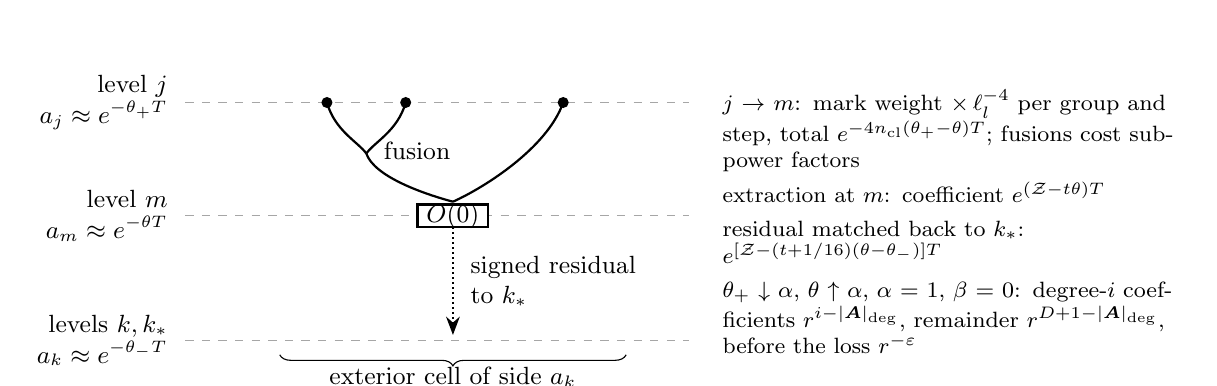
\begin{tikzpicture}[x=1cm,y=0.72cm,>=Stealth,font=\small]
\draw[gray!70,dashed] (-3.4,3) -- (3.0,3);
\draw[gray!70,dashed] (-3.4,1) -- (3.0,1);
\draw[gray!70,dashed] (-3.4,-1.2) -- (3.0,-1.2);
\node[anchor=east,align=right] at (-3.5,3) {level $j$\\ $a_j\approx e^{-\theta_+T}$};
\node[anchor=east,align=right] at (-3.5,1) {level $m$\\ $a_m\approx e^{-\theta T}$};
\node[anchor=east,align=right] at (-3.5,-1.2) {levels $k,k_*$\\ $a_k\approx e^{-\theta_-T}$};
\fill (-1.6,3) circle (2pt);
\fill (-0.6,3) circle (2pt);
\fill (1.4,3) circle (2pt);
\draw[thick] (-1.6,3) .. controls (-1.5,2.5) and (-1.2,2.3) .. (-1.1,2.1);
\draw[thick] (-0.6,3) .. controls (-0.7,2.5) and (-1.0,2.3) .. (-1.1,2.1);
\draw[thick] (-1.1,2.1) .. controls (-1.0,1.7) and (-0.4,1.4) .. (0,1.25);
\draw[thick] (1.4,3) .. controls (1.2,2.2) and (0.4,1.5) .. (0,1.25);
\node[anchor=west] at (-1.0,2.15) {fusion};
\draw[fill=white,thick] (-0.45,0.8) rectangle (0.45,1.2);
\node at (0,1.0) {$O(0)$};
\draw[->,thick,densely dotted] (0,0.8) -- (0,-1.1);
\node[anchor=west,align=left] at (0.1,-0.15) {signed residual\\ to $k_*$};
\draw[decorate,decoration={brace,mirror,amplitude=4pt}] (-2.2,-1.45) -- (2.2,-1.45);
\node at (0,-1.85) {exterior cell of side $a_k$};
\node[anchor=west,align=left,text width=5.8cm,font=\footnotesize] at (3.3,0.9) {
$j\to m$: mark weight $\times\,\ell_l^{-4}$ per group and step, total $e^{-4n_{\rm cl}(\theta_+-\theta)T}$; fusions cost subpower factors\\[3pt]
extraction at $m$: coefficient $e^{(\mathcal Z-t\theta)T}$\\[3pt]
residual matched back to $k_*$: $e^{[\mathcal Z-(t+1/16)(\theta-\theta_-)]T}$\\[3pt]
$\theta_+\downarrow\alpha$, $\theta\uparrow\alpha$, $\alpha=1$, $\beta=0$: degree-$i$ coefficients $r^{i-|\boldsymbol A|_{\deg}}$, remainder $r^{D+1-|\boldsymbol A|_{\deg}}$, before the loss $r^{-\varepsilon}$};
\end{tikzpicture}
\caption{The three scales of Lemma~\ref{lem:J-lattice}. Markers start at the insertion resolution~$a_j$, are grouped when they cease to be $B_l^2$-separated, and reach level~$m$ as one group, where one degree-$t$ field is extracted; the signed residual is matched backward to~$k_*$. Right: losses and gains up to subpower factors, at fixed truncation (no series in~$D$).}
\label{fig:J-scales}
\end{figure}

\begin{lemma}[Lattice cluster replacement]\label{lem:J-lattice}
For every output degree~$t$, the preceding configurations admit labels~$v_{N,p}^{\rm out}\in V_t$ on an ordered cutoff tail such that
\begin{align*}
\|v_{N,p}^{\rm out}\|_m&\preccurlyeq e^{(\mathcal Z-t\theta)T},\\
\left\|\prod_\iota O_{N,p}(v_\iota,x_\iota)-O_{N,p}(v_{N,p}^{\rm out},0)\right\|_{\mathcal C^{\rm tile}_k(0)}
&\preccurlyeq e^{[\mathcal Z-(t+1/16)(\theta-\theta_-)]T}.
\end{align*}
The difference is interior. The bounds are uniform in cutoff and volume on that tail.
\end{lemma}
\begin{proof}\label{proof:J-lattice-start}
The insertions are expanded in the marked format of Definition~\ref{def:D26} and Lemmas~\ref{lem:E2.2}--\ref{lem:E2.2a}; Lemmas~\ref{lem:J-signed-local} and~\ref{lem:J-marked-costs} supply the extraction once the markers form one group, and the steps below bound the mark weight lost before that. In the nilpotent variables defined above, the coefficient of their product in $\density\rho_N\prod_\iota(1+z_\iota O_{N,p}(v_\iota,x_\iota))$ is the product insertion times the density. Until level~$j$ the stencils are disjoint, so their marked integrations are separate.

Moving a marker to its representative through at most~$h$ cover balls gives
\begin{equation}\label{eq:J-support-move}
\cover(X\cup\{y_\iota:\iota\in A\})\le\cover(X)+h|A|.
\end{equation}
If at most~$\mathfrak N$ representatives occupy a ball, shrinking each affected weight by $\eta e^{-\sigma h}$ gives the original term times~$\eta^{|A|}$. In the anchored sum, terms incident on the old ball use its original majorant; any new incidence can be assigned to an old marker on the joining path. There are at most~$n_{\rm cl}$ old markers for each new representative and~$\mathfrak N$ representatives. With $\eta\le[(1+\mathfrak N)n_{\rm cl}]^{-1}$, the sum of the contributions from these assignments is bounded by the original majorant. Unmarked terms keep their supports. Hence the enlarged weighted series is bounded by the original majorant series of Lemma~\ref{lem:D1}.

Choose one input index~$\iota_0$. At each level keep a maximal $B_l^2$-separated set of representatives containing the current representative descended from~$\iota_0$, and attach each discarded point to a retained neighbor. The distinguished input need not itself lie at the origin. By the centered-block hypothesis, every input has ancestor~$0$ at level~$m+1$; in particular the retained representative has that ancestor, and the final group is extracted at~$0$. A fusion decreases the number of groups, so there are at most~$n_{\rm cl}-1$ fusions. No extra origin marker is introduced. The joining-cover bound can be taken as
$h_l=16[1+\ell_l(B_l+B_{l+1}+1)^2]^4$.
There are at most~$n_{\rm cl}$ representatives in any ball. Set
\begin{equation*}
\alpha_j=\min\left\{1,\ \min_{m\le l<j}\frac{e^{-(\sigma_{J_{l+1}}+1)h_l}}{(1+n_{\rm cl})n_{\rm cl}}\right\},
\end{equation*}
with the inner minimum omitted if the interval is empty. Then $\alpha_j/8$ is at most the factor $\eta e^{-\sigma h_l}$ required above at every fusion. The entry requirements of Section~\ref{sec:constants} and Lemma~\ref{lem:E1.1} give $(\sigma_{J_{l+1}}+1)h_l=o(s_l)$, so~$\alpha_j$ is subpower: split the maximum logarithmic cost into a fixed initial segment and a tail bounded by~$\tau s_j$, then send~$\tau$ to zero.

Between fusions the one-mark integration costs at most~$6\ell_l\le\ell_l^4$ in each weight. To derive this bound, let~$\mathfrak m$ be an incoming marked majorant. Apply the rooted clause of Lemma~\ref{lem:D-connected} coefficientwise in the submultiplicative marked norm, with the marked factor fixed. Separate the transported regular terms into the zero-jet local integration remainder, of total weighted mass~$p_l$, and the incoming regular contribution carried without Taylor subtraction.

Use the support conversion factor~$\mathcal A_l$ defined by~\eqref{eq:E-support-conversion}. For a fine support~$X$ of the unsubtracted incoming contribution, let~$Y$ be its coarse support, including the incident windows. The support conversion estimate there gives
\begin{equation*}
(\sigma_{J_l}+2)\cover_{B_l}(Y)
\le\log\mathcal A_l+\tfrac12\sigma_{J_{l+1}}\cover_{B_{l+1}}(X)\,.
\end{equation*}
Exponentiating bounds this incoming mass by~$\mathcal A_l\mathfrak m$; the remaining half of the fine exponent is nonnegative. Item~\ref{it:E-graph} of Section~\ref{sec:partII-E.1} imposes~$\mathcal A_l\le\ell_l$.

The combined regular mass is thus at most~$p_l+\mathcal A_l\mathfrak m$. Splitting a complex marked term into its real and imaginary parts costs at most twice its majorant. For the forced terms, let~$f_l$ denote their total contribution after this splitting and the normalization in~\eqref{eq:E-marked-mass}; their eligibility tests remain attached. Use the termwise bounds in the proof of Lemma~\ref{lem:E-marked-step} for the zero-jet local remainder: its regular part retains the Taylor gain, and its forced part retains half the forced suppression. The unsubtracted incoming contribution is bounded by the support conversion above; the $\eta r$ graph bound in that proof is not used for this contribution. Raising the entry coupling gives~$2p_l\le\mathfrak m$ and~$f_l\le\mathfrak m$. Adding the two contributions gives
\begin{equation*}
2(p_l+\mathcal A_l\mathfrak m)+f_l
\le(2\ell_l+2)\mathfrak m\le6\ell_l\mathfrak m.
\end{equation*}
With~$g$ groups remaining, their product weight at level~$l$ is consequently at least
\begin{equation}\label{eq:J-marker-weights}
(a_j/a_l)^{4n_{\rm cl}}(\alpha_j/8)^{n_{\rm cl}(n_{\rm cl}-g)}\prod_\iota w_\iota.
\end{equation}
Indeed a separated step multiplies the weight by~$\ell_l^{-4g}\ge\ell_l^{-4n_{\rm cl}}$. A fusion to~$g'<g$ uses at most~$n_{\rm cl}$ factors~$\alpha_j/8$, whereas $n_{\rm cl}(g-g')\ge n_{\rm cl}$.

At~$m+1$ all representatives have the same ancestor. The initial normalized-field weights can be chosen with $\prod_\iota w_\iota=e^{-W\theta_+T+o(T)}$ by Lemma~\ref{lem:E2.2}. Thus~\eqref{eq:J-marker-weights} gives $\omega=e^{-\mathcal ZT+o(T)}$ and $\mathfrak E_m=e^{(\mathcal Z-t\theta)T+o(T)}$. Choose
\begin{equation}\label{eq:J-terminal-weight}
\varpi=\exp\{[(t+1/16)(\theta-\theta_-)-\mathcal Z]T\}.
\end{equation}
The second condition of~\eqref{eq:J-marked-weights} has exponent $-(\theta-\theta_-)/16<0$; the first has exponent $-\mathcal Z-15(\theta-\theta_-)/16$, strictly below the exponent~$-\mathcal Z$ of its right side. Both therefore hold, including every subpower factor. Lemma~\ref{lem:J-marked-costs} gives the coefficient bound~$2\mathfrak E_m$ and chessboard bound~$2N_k/\varpi$ asserted here. All enlargements fit the prescribed cell margin. Reflection and conjugation preserve the majorants, so the same calculation applies to all cells and all cutoffs on the common tail.
\label{proof:J-lattice-end}
\end{proof}


We next state the bounds when the exterior distances also shrink. Write $w=\prod_i A_i(x_i)$, $W=|\boldsymbol A|_{\deg}$ and $V=|\boldsymbol B|_{\deg}$. Consider families of configurations indexed by $T\to\infty$. Suppose the cluster lies within $e^{-\alpha T+o(T)}$ of~$o$, its pairwise distances are at least $e^{-\alpha T-o(T)}$, and $\alpha>0$. Exterior points are at distance at least $e^{-\beta T-o(T)}$ from every cluster point and~$o$, and mutually at least $e^{-\upsilon T-o(T)}$ apart, where $0\le\beta<\alpha$ and $\upsilon\ge\beta$. The field lists are fixed, or range over fixed compact sets of coefficients. Call these conditions~(G). Let $u_{(i,\kappa)}$, $\kappa$ ranging over the degree-$i$ basis fields, be the biorthogonal fields of Section~\ref{sec:partII-J.1}, and put $w_o=\tau_{-o}w$. Set
\begin{align*}
\lambda_{i,\kappa}^{\rm raw}&=\sum_\gamma m_{(i,\kappa)\gamma}S(w_o,B_{i,\gamma}),\\
A^{\rm raw}_h&=P_h^{\rm raw}w_o\in F_h,\\
\mathcal R_D^{\rm raw}&=M^0\Bigl(w\prod_lB_l(y_l)\Bigr)
 -M^0\Bigl(A^{\rm raw}_D(o)\prod_lB_l(y_l)\Bigr)\in\mathfrak A_0\,.
\end{align*}
Here $P_h^{\rm raw}$ is the projection of Definition~\ref{def:D31}, and $M^0$ is the compression of Definition~\ref{def:compression} and Lemma~\ref{lem:H1.2}.

The following estimates retain the exterior distance powers needed for nested clusters and contacts.
\begin{samepage}
\begin{lemma}[Power-separated estimates]\label{lem:J-power-separated}
For every $i,D\ge0$ and $j\le h$, families of configurations obeying~(G) satisfy
\begin{align}
\lambda_{i,\kappa}^{\rm raw}&\preccurlyeq e^{(W-i)\alpha T},&
\mathcal R_D^{\rm raw}&\preccurlyeq e^{[W\alpha-(D+1)(\alpha-\beta)+V\upsilon]T},\label{eq:J-raw-rates}\\
Q_jB_jw-Q_jL_{j,h}A^{\rm raw}_h&\preccurlyeq e^{(W-h-1)\alpha T}.&&\label{eq:J-average-error}
\end{align}
The final coefficients and tested remainder of Definition~\ref{def:D33} obey the same respective bounds, in norm before state evaluation.
\end{lemma}
\end{samepage}
A degree-$i$ coordinate thus costs the cluster degree less~$i$ at the cluster height~$\alpha$, and the remainder gains $(D+1)(\alpha-\beta)$ from the difference of the cluster and exterior heights.

\begin{proof}\label{proof:J-power-start}
The proof converts chessboard seminorms into algebra norms by Lemma~\ref{lem:H-roots}, applies Lemma~\ref{lem:J-lattice} on grid configurations, removes the grid restriction by derivative descent with the calculus of Lemma~\ref{lem:F2}, and then averages the reconstruction map. Write~$n_{\rm cl}=|I_{\rm cl}|$.

\emph{Step 1: chessboard seminorms bound algebra norms.} Suppose a lattice difference has centered chessboard seminorm (Lemma~\ref{lem:E2.3}) at most~$B_{\rm rt}$, and the exterior insertions have chessboard seminorms at most~$B_{{\rm rt},l}$. Put the difference in a coarse cell and the exterior insertions in finer disjoint cells; their stencils fit by Lemma~\ref{lem:F1a}. Let~$U\in\mathfrak A_0$ be the corresponding compressed difference. The lattice paragraph after Lemma~\ref{lem:H-roots}, with the moment identity of Lemma~\ref{lem:H1.2}, gives for every~$n\in\N$
\begin{equation}\label{eq:J-moments}
\int_{\phases}|\xi(U)|^{2n}\,d\nu(\xi)
\le(B_{\rm rt}\prod_lB_{{\rm rt},l})^{2n}\,,
\end{equation}
and Lemma~\ref{lem:H-roots} gives~$\|U\|\le B_{\rm rt}\prod_lB_{{\rm rt},l}$. The same argument bounds a word by the chessboard seminorms of its insertions, giving the crude exponent~$W\alpha+V\upsilon$ on the stated geometries.

\emph{Step 2: grid configurations.} Consider the generic grid configurations defined above in a cluster of height~$\alpha>0$. Choose $0<\theta_-<\theta<\alpha<\theta_+$, with exterior distance exponent~$\beta<\theta_-$, and $\mathcal Z=W\theta_++4n_{\rm cl}(\theta_+-\theta)$. Apply Lemma~\ref{lem:J-lattice} with an auxiliary degree~$t\ge D$. For each fixed cluster geometry the output coefficients are bounded at fixed~$m$; the reverse transfer inequality of Lemma~\ref{lem:E2.2} bounds them also at the reference level. Along a refinement of the ordered cutoff tails they converge to a field~$A^{\rm out}\in F_t$. Step~1 bounds the replacement error by exponent
\begin{equation*}
\mathcal Z-(t+1/16)(\theta-\theta_-)+V\upsilon\,.
\end{equation*}
Testing the same difference against the fixed probes bounds the raw coordinate errors. Reference-level coefficient convergence and Lemma~\ref{lem:J-graded-quotient} apply on this geometry-dependent refinement. The degree-$i$ raw coordinate annihilates~$F_{i-1}$ by the biorthogonality before Definition~\ref{def:D31}, and is a fixed bounded functional on the quotient. With~$\epsilon_{\rm bd}\preccurlyeq e^{(\mathcal Z-t\theta)T}$, \eqref{eq:J-graded-input} therefore bounds that coordinate by exponent~$\mathcal Z-i\theta$.

Choose~$t$ large enough that $(t+1/16)(\theta-\theta_-)\ge(D+1)\theta$ and also large enough for every coefficient being tested. Exact reconstruction of~$A^{\rm out}$ by the prescription separates the degrees~$i\le D$ from~$D<i\le t$. An omitted degree contributes at most
\begin{equation*}
\mathcal Z-i\theta+i\beta+V\upsilon\le \mathcal Z-(D+1)(\theta-\beta)+V\upsilon\,.
\end{equation*}
The low-degree coordinate errors satisfy the same bound, by the chosen auxiliary horizon. We have therefore proved grid exponents~$\mathcal Z-i\theta$ for raw degree-$i$ coordinates and~$\mathcal Z-(D+1)(\theta-\beta)+V\upsilon$ for the raw remainder.

\emph{Step 3: derivative descent.} Run the crude, grid and derivative bounds uniformly over all characters~$\xi\in\phases$. The algebra~$\mathfrak A_0$ is commutative, so $\|U\|=\sup_\xi|\xi(U)|$. The identities of Lemmas~\ref{lem:F2}, \ref{lem:H1.1} and~\ref{lem:H1.3} hold throughout any separated neighborhood: differentiating a cluster position replaces that slot by its positional derivative, also after compression and character evaluation. For each compact rounding segment, a common translation places the words in fixed slabs with positive buffers, so the slab norm identity applies along the whole segment. For the raw remainder this differentiates the \emph{varying} field $A_D^{\rm raw}=D_D((S(w_o,B_{D,\gamma}))_\gamma)$ as well as the original cluster. Since the probes, decoder, center and exterior word are fixed, linearity gives
\begin{equation*}
 \partial_{x_i^a}A_D^{\rm raw}(w_o)
 =A_D^{\rm raw}\bigl((\partial_{i,a}w)_o\bigr).
\end{equation*}
Consequently the derivative of the raw remainder is the raw remainder for the word with this differentiated slot. The center need not be distinct from the cluster points: the original word and the center-insertion word are separate correlations. Assign the differentiated slot degree $d_i+1$, even if its class vanishes or admits a lower-degree representative.

For suitable constants~$c_0,d_0$ independent of the input degrees, the crude bound has exponent~$\alpha W+c_0$ and the grid bound exponent~$\theta_+W+d_0$. We descend in the total assigned input degree~$W$. The crude bound proves the desired estimate for all~$W$ with $(\theta_+-\alpha)W\ge c_0-d_0$, because $\theta_+>\alpha$. For the induction step, move the configuration to a generic level-$j$ grid configuration a distance $O(a_j)$ away. Since $a_j=e^{-\theta_+T+o(T)}$ and $\beta<\alpha<\theta_+$, the entire intervening segment lies in a separated neighborhood with the same cluster and exterior exponents, and remains clear of the fixed probes; spectator--spectator distances do not change. The slot identity therefore applies at every point of the segment. For any fixed positive slack, failure of a uniform segment bound would give a violating sequence of segment points and characters, still satisfying~(G), contrary to the induction hypothesis. The induction hypothesis and grid spacing give $e^{[\theta_+(W+1)+d_0]T+o(T)}a_j=e^{(\theta_+W+d_0)T+o(T)}$: the displacement error has exactly the required degree-$W$ bound, for every slot and axis.

\emph{Step 4: limits.} Now let~$\theta\uparrow \alpha$ and~$\theta_+\downarrow \alpha$, keeping~$\beta<\theta_-<\theta$. Translation moves the origin to~$o$. This proves~\eqref{eq:J-raw-rates} for arbitrary configurations. The remainder estimate is in~$\mathfrak A_0$, and empty clusters give zero remainder.

\emph{Step 5: the coefficients of Definition~\ref{def:D33}.} Let~$A^{\rm raw}_h\in F_h$ be the raw truncation at an auxiliary degree~$h$. In every rotated probe correlation, the difference between the cluster and~$A^{\rm raw}_h(0)$ has exponent~$(W-h-1)\alpha$. The marked norm bounds and multilinearity make~\eqref{eq:J-raw-rates} uniform on compact coefficient sets, hence on the rotation orbit. Haar averaging, conjugation and the fixed maps~$Q_j$ preserve the exponent. This proves~\eqref{eq:J-average-error}. With~$h=j$, all lower raw modes vanish under~$Q_jL_{j,j}$ by~\eqref{eq:J-cuts}; the remaining modes have exponent~$(W-j)\alpha$. With~$h=D$, use~\eqref{eq:J-cuts} to reconstruct~$A^{\rm raw}_D$, and telescope the raw remainder with the errors~\eqref{eq:J-average-error} for~$j\le D$. Testing an error in~$F_j$ costs~$j\beta+V\upsilon$, so their largest exponent is~$W\alpha-(D+1)(\alpha-\beta)+V\upsilon$.
\label{proof:J-power-end}
\end{proof}

At fixed exterior distances the power-separated estimates become the bounds of Theorem~\ref{prop:OP}. The parameters~$M_{\rm geo}$ are nonnegative and the separation and error parameters are positive, as in Definition~\ref{def:D18}. For the algebra-valued remainder put
\begin{equation*}
\mathcal R_D=M^0\Bigl(\prod_i A_i(x_i)\prod_l B_l(y_l)\Bigr)
-\sum_{j\le D,\,\lambda\in\channels{j}}c_{j,\lambda}\,
 M^0\Bigl(O_{j,\lambda}(o)\prod_l B_l(y_l)\Bigr).
\end{equation*}
Here~$M^0$ is the compression of separated words of Definition~\ref{def:compression} and Lemma~\ref{lem:H1.2}; its characters and vacuum state give the phase and mixed remainders~$\mathcal R_D^\zeta$ of Definition~\ref{def:D18}.

\begin{lemma}[Compressed remainder bound]\label{lem:J1.2}
Fix finite lists $\boldsymbol A,\boldsymbol B$, $M_{\rm geo}\ge0$, $\eta,\delta_{\rm sp},\varepsilon>0$ and $D\in\N$. There is $r_1>0$ such that, for $0<r<r_1$, every $(r,M_{\rm geo},\eta)$-cluster $(x,o)$ and every $\delta_{\rm sp}$-clear spectator configuration~$y$,
\begin{equation*}
\|\mathcal R_D\|_{\mathfrak A_0}\le r^{D+1-|\boldsymbol A|_{\deg}-\varepsilon}\,.
\end{equation*}
\end{lemma}

\begin{proof}\label{proof:J1.2-start}
Apply Lemma~\ref{lem:J-power-separated} to Definition~\ref{def:D18}, with $T=-\log r$, $\alpha=1$ and $\beta=\upsilon=0$. Every admissible configuration has these bounds on extent and reciprocal distances. If the claimed threshold failed, choose violating configurations at radii tending to zero. The estimate just proved along that sequence, with loss~$\varepsilon/2$, eventually contradicts the violation with loss~$\varepsilon$: constants and subpower factors are absorbed by~$r^{\varepsilon/2}$. Taking~$M_{\rm geo}r<\delta_{\rm sp}/2$ also ensures separation.
\label{proof:J1.2-end}
\end{proof}

\begin{proof}[Proof of Theorem~\ref{prop:OP}]
Lemma~\ref{lem:J1.1} fixes the fields and coefficients of Definition~\ref{def:D18} before spectators, state indices or truncation. The coefficient bound follows from the coefficient estimate of Lemma~\ref{lem:J-power-separated} by the contradiction argument in the proof of Lemma~\ref{lem:J1.2}; its threshold depends only on the data of the coefficient. Character evaluation and the mixed vacuum are contractions on~$\mathfrak A_0$, so Lemma~\ref{lem:J1.2} gives the remainder bound with its own threshold. The argument bounds~$\mathcal R_D$ in~$\mathfrak A_0$ before state evaluation.
\end{proof}

A nested configuration retains leaf positions and internal centers, so it also describes partially replaced words. Call an internal vertex other than the root proper, and fix its truncation~$D_v\in\N$.

\begin{samepage}
\begin{definition}[Nested geometry and rates]\label{def:D34}
Give each vertex~$v$ of a finite rooted tree a position~$z_v$, each leaf a field~$A_i$, and each internal vertex a scale~$\varrho_v>0$. Its root~$o_{\rm root}$ is internal. Require $\varrho_{o_{\rm root}}=r$, $\varrho_v\le\varrho_{\operatorname{par}(v)}$, $|z_u-z_v|\le M_{\rm geo}\varrho_v$ for every descendant~$u$, and $|z_u-z_{u'}|\ge\eta\varrho_v$ for positions in different child subtrees. Put
\begin{align*}
W_v&=\sum_{i\text{ below }v}\deg A_i,&q_v&=\varrho_v/\varrho_{\operatorname{par}(v)},\\
\mathcal Q_{\varepsilon,q}(\varrho)&=r^{q-W_{o_{\rm root}}-\varepsilon}
\prod_{v\ne o_{\rm root}\text{ internal}}q_v^{-W_v-\varepsilon},&
\mathsf e_{\boldsymbol D}(\varrho)&=\sum_{v\ne o_{\rm root}\text{ internal}}q_v^{D_v+1}\,.
\end{align*}
\end{definition}
\end{samepage}
Spectators are~$\delta_{\rm sp}$-clear of every tree position and each other.

The recursion retains every leaf, including those above a neighboring truncation.

\begin{samepage}
\begin{definition}[Iterated coefficient]\label{def:D35}
A leaf contributes its field and coefficient one. At a proper internal vertex~$v$, replace its children by
\begin{equation*}
\sum_{j\le D_v}\sum_{\lambda\in\channels{j}}
 c_{j,\lambda}(\text{child fields};\text{child centers},z_v)O_{j,\lambda},
\end{equation*}
multiplying their coefficients and summing. At the root retain only~$(q,\lambda)$, giving~$C^{\rm it,\boldsymbol D}_{q,\lambda}$. The direct coefficient is $C^{\rm dir}_{q,\lambda}=c_{q,\lambda}(\boldsymbol A;z_{\rm leaves},z_{o_{\rm root}})$. This compares successive and direct expansion.
\end{definition}
\end{samepage}

For example, let a cluster~$v$ of leaves of total degree~$W_v$ first fuse at scale~$\varrho_v$, and let its output then fuse with the remaining leaves at the root scale~$r$. If~$v$ is the only proper internal vertex, then
\begin{equation*}
\mathcal Q_{\varepsilon,q}=r^{q-W_{o_{\rm root}}-\varepsilon}(\varrho_v/r)^{-W_v-\varepsilon},
\qquad \mathsf e_{\boldsymbol D}=(\varrho_v/r)^{D_v+1}.
\end{equation*}
The first factor is the size allowed for the direct coefficient; the second is the truncation gain at the inner fusion. For a general tree the errors from different vertices are added, as in the definition of~$\mathsf e_{\boldsymbol D}$.

Fix the tree, leaf list, output~$(q,\lambda)$, proper-vertex truncations, $M_{\rm geo}\ge0$ and~$\eta,\varepsilon>0$. No lower bound on the ratios~$q_v$ is imposed.

\begin{lemma}[Nested coefficient estimate]\label{lem:J1.4}
There is~$r_0>0$ such that all geometries of Definition~\ref{def:D34} with~$0<r<r_0$ satisfy
\begin{equation*}
|C^{\rm dir}_{q,\lambda}|\le\mathcal Q_{\varepsilon,q},\qquad
|C^{\rm dir}_{q,\lambda}-C^{\rm it,\boldsymbol D}_{q,\lambda}|
\le\mathcal Q_{\varepsilon,q}\mathsf e_{\boldsymbol D}\,.
\end{equation*}
Both expressions are smooth in neighborhoods of these geometries.
\end{lemma}

\begin{proof}\label{proof:J1.4-start}
The estimates of Lemma~\ref{lem:J-power-separated} are applied vertex by vertex along a tree induction, after reducing to sequences whose scales have convergent logarithmic heights. Along any sequence of admissible radii and scales tending to the root collision, put $T=\sum_{v\text{ internal}}\log(1/\varrho_v)$. Eventually every summand is positive. After a subsequence, $\log(1/\varrho_v)/T\to a_v\ge0$, with~$\sum_va_v=1$ and~$a_v\ge a_{\operatorname{par}(v)}$. Set
\begin{equation*}
\mathcal B=W_{o_{\rm root}}a_{o_{\rm root}}
+\sum_{v\ne o_{\rm root}\text{ internal}}W_v(a_v-a_{\operatorname{par}(v)})\,.
\end{equation*}
We prove by induction on the tree that a direct output of degree~$q$ has exponent~$\mathcal B-qa_{o_{\rm root}}$, and its error against the prescribed finite iteration has that exponent minus $\gamma=\min_{v\ne o_{\rm root}\text{ internal}}(D_v+1)(a_v-a_{\operatorname{par}(v)})$.
With no proper internal vertices the two coefficients coincide exactly.

First flatten the edges~$u\to v$ with~$a_u=a_v$: combine their grouping before making any field replacement. The word at~$v$ then consists of original leaves in this equal-height component and outputs from strictly finer children; its distinct positions are separated at exponent~$a_v$ by the tree geometry. For a child with~$a_u>a_v$, expand to an auxiliary horizon~$H_u$. The remainder exponent has the improvement~$(H_u+1)(a_u-a_v)$ by~\eqref{eq:J-raw-rates}. Choose the children in a fixed order, choosing~$H_u$ only after the outputs already used as exterior fields are fixed. Each improvement tends to infinity with~$H_u$, whereas the exterior degree in that step is fixed. It can therefore exceed any prescribed error exponent. The identity
\begin{equation}\label{eq:J-telescope}
\prod_{i=1}^nX_i-\prod_{i=1}^nY_i
=\sum_{i=1}^n\left(\prod_{h<i}Y_h\right)(X_i-Y_i)
                    \left(\prod_{h>i}X_h\right)
\end{equation}
justifies these successive replacements in every correlation and in every probe defining a coefficient. It is an identity of separated expressions, with their scalar coefficient factors retained.

For a fixed collection of child outputs~$j_u$, the child exponents include~$-j_ua_u$, and the parent coefficient contributes~$j_ua_v$. Their sum contains~$-j_u(a_u-a_v)$; the remaining leaf weights telescope to~$\mathcal B-qa_{o_{\rm root}}$. Nonnegative output degrees therefore never increase this exponent. If the root height is zero, apply the crude estimate to this root word of child outputs; its finitely many field degrees cost exponent zero, while their coefficients already carry the child contributions to~$\mathcal B$. This proves the direct bound, by the preceding arbitrary-accuracy replacements and the induction hypothesis. Remove auxiliary outputs above~$D_u$. Each discarded term has at least one~$j_u\ge D_u+1$ and thus gains at least~$\gamma$. Replacing the remaining direct child coefficients by their iterated coefficients uses~\eqref{eq:J-telescope} again and gains~$\gamma$ from one child error. If~$\gamma=0$, the direct and iterated bounds themselves give the error exponent. If~$\gamma>0$, every proper internal scale increase is positive and the auxiliary horizons can be chosen to make the preceding replacement errors smaller than this exponent. This proves the induction for the difference, with one improvement rather than a product of improvements.

The logarithmic exponent of~$\mathcal Q_{\varepsilon,q}$ is
\begin{equation*}
\mathcal B-qa_{o_{\rm root}}+\varepsilon A_*,\qquad
A_*=a_{o_{\rm root}}+\sum_{v\ne o_{\rm root}\text{ internal}}(a_v-a_{\operatorname{par}(v)})>0\,.
\end{equation*}
Positivity follows because~$\sum_va_v=1$: if every displayed nonnegative term vanished, every~$a_v$ would vanish. The exponent of~$\mathsf e_{\boldsymbol D}$ is~$-\gamma$. Thus the estimates with loss~$\varepsilon/2$ imply the displayed bounds with loss~$\varepsilon$ and coefficient one along this sequence. A sequence of violations would have the subsequence just treated, a contradiction. This proves a threshold uniform in the scale vector, even when some scales decrease faster than every power of~$r$. The positions in each word evaluated by the recursion stay separated and, for small~$r$, clear of its finite rotated probe family. A center may coincide with a descendant appearing in a different word. The averaging integrands are smooth on an open neighborhood with that clearance; their derivatives are bounded on compact neighborhoods times~$O(4)$. Differentiating the finite sums and Haar integrals proves smoothness.\qedhere
\label{proof:J1.4-end}
\end{proof}

For tested products, retain the original leaves at the root; only the degree of its output is truncated. Fix additionally the root truncation~$m\in\N$, a spectator list~$\boldsymbol B$ and~$\delta_{\rm sp}>0$.

\begin{lemma}[Nested tested estimate]\label{lem:J1.5}
For some~$r_0>0$, every smaller radius, admissible nested geometry, admissible spectator configuration and state index~$\zeta$ satisfy
\begin{equation*}
|\mathcal R_m^\zeta(\boldsymbol A,z_{\rm leaves};\boldsymbol B,y;z_{o_{\rm root}})|
\le\mathcal Q_{\varepsilon,m+1}(\varrho)\,.
\end{equation*}
The same bound holds in the norm of~$\mathfrak A_0$ before evaluation in a character or the mixed vacuum.
\end{lemma}

\begin{proof}
The tree induction of Lemma~\ref{lem:J1.4} is run with the spectators kept in every replacement of Definition~\ref{def:D18}. Their reciprocal distances from every tree position and from one another have exponent zero. They therefore add no term to~$\mathcal B$. After the arbitrary-accuracy child replacements, the root remainder estimate of Lemma~\ref{lem:J-power-separated} has exponent~$\mathcal B-(m+1)a_{o_{\rm root}}$. When~$a_{o_{\rm root}}=0$, apply the crude bound to the root word of child outputs after these replacements. The child coefficient powers already account for~$\mathcal B$; the finitely many root output fields and the spectators cost exponent zero. The positive quantity~$\varepsilon A_*$ used above again absorbs all finite sums and subpower factors. The contradiction argument is unchanged. The norm estimate follows from~\eqref{eq:J-moments}; applying a character or the mixed vacuum proves the scalar bounds with the same threshold.
\end{proof}

\begin{remark}[Integrated forms]\label{lem:J1.3}\label{lem:J1.6}
The thresholds of Lemmas~\ref{lem:J1.2}, \ref{lem:J1.4} and~\ref{lem:J1.5} precede positions, scale vectors and states, so they survive integration. Fix the data of one of these lemmas, a measurable space~$Z$ and~$B_0\ge0$. Below a threshold preceding the measure, the weight, the scale vector and the maps, the following holds. Let $\lambda_Z$ be a measure on~$Z$, $\vartheta_Z$ an integrable complex weight with $\int|\vartheta_Z|\,d\lambda_Z\le B_0$, and the geometry, spectator and phase maps almost-everywhere measurable and admissible almost everywhere on~$\{\vartheta_Z\ne0\}$; in the nested case the scale vector~$\varrho$ is fixed throughout the integral. Then the weighted full, truncated and compared expressions are integrable, and
\begin{align*}
\Bigl|\int_Z\vartheta_Z\mathcal R_D^{\xi(z)}\,d\lambda_Z\Bigr|&\le B_0r^{D+1-|\boldsymbol A|_{\deg}-\varepsilon},&
\Bigl|\int_Z\vartheta_ZC^{\rm dir}_{q,\lambda}\,d\lambda_Z\Bigr|&\le B_0\mathcal Q_{\varepsilon,q},\\
\Bigl|\int_Z\vartheta_Z\bigl(C^{\rm dir}_{q,\lambda}-C^{\rm it,\boldsymbol D}_{q,\lambda}\bigr)\,d\lambda_Z\Bigr|&\le B_0\mathcal Q_{\varepsilon,q}\mathsf e_{\boldsymbol D},&
\Bigl|\int_Z\vartheta_Z\mathcal R_m^{\xi(z)}\,d\lambda_Z\Bigr|&\le B_0\mathcal Q_{\varepsilon,m+1}.
\end{align*}
The first and last bounds also hold for the mixed state. Indeed, for fixed~$r$ and~$\varrho$, \eqref{eq:J-moments} bounds the full correlation uniformly, and the truncated sum is the full expression minus the bounded remainder. Smoothness of the coefficients where their rotated probes are clear, continuity in the phase (Lemma~\ref{lem:H1.3}) and rounding of the geometry to a countable dense set give joint measurability. Integrating the pointwise bounds against~$|\vartheta_Z|$ gives the estimates.
\end{remark}

\subsection{Contact subtractions}\label{sec:partII-J.2}

Property~E7 alone gives some extension through the collision diagonals (see the discussion before Theorem~\ref{prop:CT}). This subsection constructs a specific one, by explicit subtraction of normal Taylor jets of the test function read through contact projections, and proves its local order $(2+|\boldsymbol A|_{\deg})n$ on compact sets. For each retained field degree we subtract a jet of a different order, and partial collisions require the same operation inside each smaller cluster; absolute convergence follows by summing normal shells.

We work with finite sums of field words, identifying~$A(x)$ with~$(\jmath_{d,e}A)(x)$ and imposing linearity in~$A$. Their product is concatenation. The correlation of a word is read only at distinct positions; elsewhere give it value zero. This convention is used inside the algebraic formulas below, before any integration. The underlying prescription and its fields are those fixed in Lemma~\ref{lem:J1.1}; the finite probes chosen next are independent of its OPE probes.

\begin{definition}[Contact projection]\label{def:D36}
On the same mixed hierarchy and field prescription as Lemma~\ref{lem:J1.1}, fix at each degree~$q$ a finite family of separated mixed correlation probe words whose responses distinguish the fields in~$F_q$. Such a family exists by the all-spectator null quotient and the finite-dimensional separation argument preceding Definition~\ref{def:D31}. The responses define an injective map $F_q\to\C^{\mathcal P_q^{\rm ct}}$; fix a linear left inverse, the contact decoder. Unlike Definition~\ref{def:D31}, no cross-grade biorthogonality is required. Fix an aperture~$\rho_q^{\rm ct}>0$ at most half the distance of each probe point from zero; if no probe has points, choose any positive aperture. These contact choices are fixed together on this hierarchy. For a word~$w$, set
\begin{equation*}
K_qw=\mathbf1_{\{\text{all positions of }w\text{ lie in }\overline B(0,\rho_q^{\rm ct})\}}w\,.
\end{equation*}
Apply the averaging and reality formula of Definition~\ref{def:D32} to this clipped word with the contact probes; extend linearly to sums, obtaining~$B_q^{\rm ct}$. This extracts contact fields on a fixed region clear of its probes.
\end{definition}

For contact expressions~$I_qA=A(0)$ still denotes a single field. Unlike the domain restriction in Definition~\ref{def:D32}, clipping here acts on each monomial before summing it.

\begin{samepage}
\begin{definition}[Coherent contact projections]\label{def:D37}
Put $T_q=P_qI_{q+1}$ and define recursively
\begin{equation*}
P_0=B_0^{\rm ct},\qquad
P_{q+1}=\jmath_{q,q+1}P_q+(1-\jmath_{q,q+1}T_q)B_{q+1}^{\rm ct},\qquad
P_{\le q}^{\rm ct}(o)w=P_q(\tau_{-o}w)\,.
\end{equation*}
The first term retains the degrees already chosen through~$q$; the second takes the new measurement and removes its component in~$\jmath_{q,q+1}F_q$. In particular, $P_{\le q}^{\rm ct}(o)[A(o)]=A$ for~$A\in F_q$.
\end{definition}
\end{samepage}

\begin{definition}[Contact grades and clearance]\label{def:D38}
The exact-degree components and common clearance are
\begin{align*}
P_{=0}^{\rm ct}(o)w&=B_0^{\rm ct}(\tau_{-o}w),\\
P_{=q}^{\rm ct}(o)w&=(1-\jmath_{q-1,q}T_{q-1})B_q^{\rm ct}(\tau_{-o}w)\quad(q>0),\\
\delta_q^{\rm pres}&=\min_{0\le d\le q}\rho_d^{\rm ct}\,.
\end{align*}
These give the graded contact subtractions and their common range of separated evaluation.
\end{definition}

The projections are defined before any test function or state. Their strata are the contact degree subspaces $E_0^{\rm ct}=F_0$ and $E_q^{\rm ct}=\ker T_{q-1}\subset F_q$ $(q>0)$. The proof of the next lemma shows that $F_q=\jmath_{q-1,q}F_{q-1}\oplus E_q^{\rm ct}$; these strata, not the complements~$E_q$ of Definition~\ref{def:D33}, carry the real bases of the contact construction.

\begin{lemma}[Real bases]\label{lem:J2.1}
The contact projections are covariant under translations, $O(4)$ and conjugation. Each contact stratum~$E_q^{\rm ct}$ has a real basis, and the degree-zero basis contains the unit.
\end{lemma}

\begin{proof}
The inclusions, rotations and conjugation of Part~I act as in Lemma~\ref{lem:J1.1}. A ball centered at zero is rotation invariant. Haar invariance proves rotation covariance of~$B_q^{\rm ct}$, and its reality formula proves conjugation covariance. These maps fix~$A(0)$: before averaging the reconstruction map returns~$R_q(h^{-1})A$, and after multiplication by~$R_q(h)$ it returns~$A$. The recursion gives
\begin{equation}\label{eq:J-contact-split}
P_qI_q=1,\qquad T_q\jmath_{q,q+1}=1,\qquad T_qP_{q+1}=P_q,\qquad
P_{\le q}^{\rm ct}(o)=\sum_{d\le q}\jmath_{d,q}P_{=d}^{\rm ct}(o)\,.
\end{equation}
For the third identity, apply~$T_q$ to the recursion and cancel~$T_qB_{q+1}^{\rm ct}$; the fourth follows by iteration. By the second identity, $1-\jmath_{q-1,q}T_{q-1}$ projects~$F_q$ onto $\ker T_{q-1}$ along $\jmath_{q-1,q}F_{q-1}$, which proves the splitting. Each stratum is invariant under conjugation and rotations. Lemma~\ref{lem:J1.1} gives real bases; choose the unit in~$F_0$. Covariance passes through the recursion, with translations following from $\tau_{-(o+u)}\tau_u=\tau_{-o}$.
\end{proof}

We give the finite subtraction formula before proving its convergence. Fix~$\boldsymbol A\in\mathbb F^n$, put~$d_i=\deg A_i$, $W=\sum_id_i$, and choose
\begin{equation*}
r_* =\min(1,\delta_W^{\rm pres}),\qquad s_*=r_*/4\,.
\end{equation*}
Lemma~\ref{lem:J2.2} uses only this single length~$s_*$. Expand each input in the contact stratum bases using~\eqref{eq:J-contact-split}, retaining its original degree tag~$d_i$ in every subtraction order. For~$h\subset\{1,\ldots,n\}$, $|h|\ge2$, let~$\Delta_h$ be its collision diagonal, $x_h^\perp$ the orthogonal component normal to~$\Delta_h$, and~$\bar x_h=|h|^{-1}\sum_{i\in h}x_i$. Thus~$x_h^\perp$ has entries~$x_i-\bar x_h$ on~$h$ and zero elsewhere. Write
\begin{equation*}
d_h=\sum_{i\in h}d_i,\qquad n^\perp_h=4(|h|-1),\qquad L_h=\max(0,d_h+1-n^\perp_h)\,.
\end{equation*}
Here $n^\perp_h$ is the dimension of the normal space of~$\Delta_h$. Fix one smooth radial cutoff $\chi(z)=\chi_0(|z|^2)$, where $\chi_0$ equals one on $[0,1]$ and zero on $[4,\infty)$. The normal Taylor operator is
\begin{equation}\label{eq:J-normal-Taylor}
(\mathrm{Tay}_{h,k}^{\perp}f)(x)=\chi(x_h^\perp/s_*)
\sum_{l=0}^k\frac1{l!}D^lf(x-x_h^\perp)[x_h^\perp,\ldots,x_h^\perp]\,.
\end{equation}
It subtracts only normal variables, leaving the centroid and all exterior variables as parameters.

An expression~$F\otimes U$ means the field expression~$F(x)$ multiplied by~$(Uf)(x)$ when tested against~$f$. Products compose the test operators. On a monomial write~$F=F_hF_{h^c}$ for its factors in and outside~$h$. Let~$\mathsf R_{h,q}$ replace the subword of~$F(x)$ on~$h$ by the field~$P_{=q}^{\rm ct}(\bar x_h)F_h(x)$ at~$\bar x_h$, leaving its test operator unchanged.

For two insertions, $h=\{1,2\}$, the centroid $o=\bar x_h$ and the relative coordinate $x_1-x_2$ parametrize~$\R^8$, and $x_h^\perp=\tfrac12(x_1-x_2,x_2-x_1)$. With $F=A_1(x_1)A_2(x_2)$ the subtracted expression is
\begin{equation*}
\Pi_h^{\rm full}f
=Ff-\sum_{q<L_h}
\bigl[P_{=q}^{\rm ct}(o)F\bigr](o)\,
\mathrm{Tay}_{h,L_h-1-q}^{\perp}f,\qquad L_h=\max(0,d_1+d_2-3).
\end{equation*}
The retained field degree~$q$ determines how many normal derivatives of the test are subtracted. On a shell $|x_h^\perp|\asymp\rho$, the degree-$q$ component has size~$\rho^{q-d_h}$ up to a loss~$\rho^{-\varepsilon'}$, the Taylor remainder of~$f$ through order $L_h-1-q$ is~$O(\rho^{L_h-q})$, and the shell has normal volume of order~$\rho^{4}$. If $L_h>0$, the two arms of the signed expression, the field minus its projected components times~$f$ and the projected components times the Taylor remainder, contribute $O(\rho^{4+L_h-d_h-\varepsilon'})$ per shell, with $4+L_h-d_h=1$. If $L_h=0$, the projection sum is empty and the remaining arm has the same bound with $4-d_h\ge1$. Thus for $0<\rho\le1$ the contribution is $O(\rho^{1-\varepsilon'})$, summable over dyadic~$\rho$ when $\varepsilon'<1$. The individual terms need not be integrable: for $d_h\ge4$ the term~$Ff$ alone is only $O(\rho^{4-d_h-\varepsilon'})$ per shell, so each subtraction must stay with the term it subtracts.

In general, define recursively
\begin{align}\label{eq:J-contact-recursion}
\mathcal C_{\{i\}}^{\rm ct}&=A_i(x_i)\otimes1,&
\Pi_h^{\rm punct}&=\sum_{\substack{\pi\text{ partition of }h\\|\pi|\ge2}}
                         \prod_{b\in\pi}\mathcal C_b^{\rm ct},\\
\mathcal C_h^{\rm ct}&=-\sum_{q<L_h}\mathsf R_{h,q}\Pi_h^{\rm punct}\,
                         \mathrm{Tay}_{h,L_h-1-q}^{\perp},&
\Pi_h^{\rm full}&=\Pi_h^{\rm punct}+\mathcal C_h^{\rm ct}\quad(|h|\ge2)\,.\notag
\end{align}
Singleton and empty full expressions are respectively~$A_i(x_i)\otimes1$ and the unit. In a nested term, the parent Taylor operator acts first on the test and the child operators act afterwards: if $b\subsetneq h$ are a child and its parent, with Taylor orders $k_b,k_h$, the resulting test factor is
\begin{equation*}
\mathrm{Tay}_{b,k_b}^{\perp}\bigl(\mathrm{Tay}_{h,k_h}^{\perp}f\bigr),
\end{equation*}
so the parent operator is written on the right. Operators on disjoint slot sets commute; no commutation is asserted for nested subsets. The recursion terminates because every child has fewer slots; expanding it gives forests of disjoint or nested collision subsets. This is a position-space forest formula. Subtracting a Taylor jet of the test function at a diagonal is, in the normal variables, the extension procedure of~\cite[Section~5.2, Theorem~5.3]{BrunettiFredenhagen2000}; here the subtracted jets are paired with contact projections, and the recursion organizes the partial collisions.

For three insertions the expression before the total-collision subtraction is
\begin{equation*}
\Pi_{\{1,2,3\}}^{\rm punct}
=A_1A_2A_3+\mathcal C_{\{1,2\}}^{\rm ct}A_3
+\mathcal C_{\{1,3\}}^{\rm ct}A_2+\mathcal C_{\{2,3\}}^{\rm ct}A_1,
\end{equation*}
with the test operators in each~$\mathcal C^{\rm ct}$ retained. The total-collision subtraction is applied to this complete expression. Its nested terms have the form $\mathsf R_{\{1,2,3\},q}\mathsf R_{\{1,2\},q'}(A_1A_2A_3)$ with test factor $\mathrm{Tay}^\perp_{\{1,2\},k'}(\mathrm{Tay}^\perp_{\{1,2,3\},k}f)$. Where $|x_1-x_2|$ is much smaller than the distance to~$x_3$, the child arms make the expression integrable in the normal variable of~$\Delta_{\{1,2\}}$, and the parent arms then treat the total collision. Figure~\ref{fig:J-forests} shows both examples.

\begin{figure}[htbp]
\centering
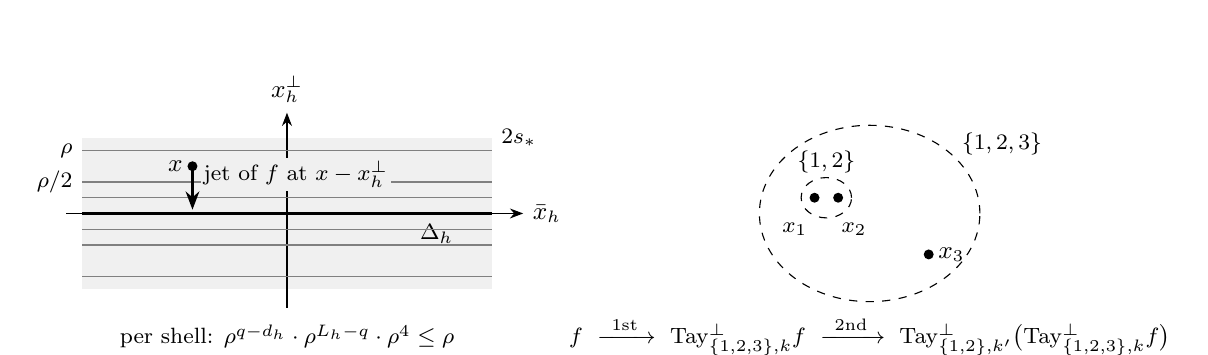
\begin{tikzpicture}[x=1cm,y=0.8cm,>=Stealth,font=\small]
\begin{scope}
\fill[gray!12] (-2.6,-1.2) rectangle (2.6,1.2);
\draw[->] (-2.8,0) -- (3.0,0) node[right] {$\bar x_h$};
\draw[->] (0,-1.5) -- (0,1.6) node[above] {$x_h^\perp$};
\draw[very thick] (-2.6,0) -- (2.6,0);
\node[anchor=north,font=\footnotesize] at (1.9,-0.02) {$\Delta_h$};
\foreach \r in {0.25,0.5,1.0} {\draw[gray] (-2.6,\r) -- (2.6,\r); \draw[gray] (-2.6,-\r) -- (2.6,-\r);}
\node[anchor=east,font=\footnotesize] at (-2.6,1.0) {$\rho$};
\node[anchor=east,font=\footnotesize] at (-2.6,0.5) {$\rho/2$};
\node[anchor=west,font=\footnotesize] at (2.6,1.2) {$2s_*$};
\fill (-1.2,0.75) circle (1.8pt) node[left] {$x$};
\draw[->,thick] (-1.2,0.72) -- (-1.2,0.06);
\node[anchor=west,fill=gray!12,inner sep=1pt,font=\footnotesize] at (-1.1,0.62) {jet of $f$ at $x-x_h^\perp$};
\node[align=center,font=\footnotesize] at (0,-1.95) {per shell: $\rho^{q-d_h}\cdot\rho^{L_h-q}\cdot\rho^{4}\le\rho$};
\end{scope}
\begin{scope}[xshift=7.4cm]
\draw[dashed] (0,0) circle (1.4);
\draw[dashed] (-0.55,0.25) circle (0.32);
\fill (-0.7,0.25) circle (1.8pt);
\fill (-0.4,0.25) circle (1.8pt);
\node[font=\footnotesize] at (-0.95,-0.25) {$x_1$};
\node[font=\footnotesize] at (-0.2,-0.25) {$x_2$};
\fill (0.75,-0.65) circle (1.8pt) node[right] {$x_3$};
\node[font=\footnotesize] at (-0.55,0.82) {$\{1,2\}$};
\node[font=\footnotesize,anchor=west] at (1.05,1.1) {$\{1,2,3\}$};
\node[align=center,font=\footnotesize] at (0,-1.95) {$f\ \xrightarrow{\ 1\text{st}\ }\ \mathrm{Tay}^\perp_{\{1,2,3\},k}f\ \xrightarrow{\ 2\text{nd}\ }\ \mathrm{Tay}^\perp_{\{1,2\},k'}\bigl(\mathrm{Tay}^\perp_{\{1,2,3\},k}f\bigr)$};
\end{scope}
\end{tikzpicture}
\caption{Left: two insertions; the test is Taylor expanded in~$x_h^\perp$ at~$\Delta_h$ where $|x_h^\perp|\le2s_*$, and each dyadic shell contributes at most~$\rho$, up to~$\rho^{-\varepsilon'}$. Right: a nested forest; the parent operator acts on the test first, and only operators on disjoint slot sets commute. Both are subtractions of separated correlations, not lattice limits at coincident points.}
\label{fig:J-forests}
\end{figure}

Before summing shells we need estimates for complete signed expressions after child subtractions. Normalize $T\to\infty$ so that all separation heights lie in~$[0,1]$, and fix a finite set~$\mathcal P$ of position paths. A finite separated sum of cost~$c$ at height~$s$ has terms
\begin{equation*}
a(T)\prod_\iota A_\iota(x_\iota(T)),\qquad
|a|\preccurlyeq e^{(c-s\sum_\iota\deg A_\iota)T},\qquad
|x_\iota-x_{\iota'}|\ge e^{-sT-o(T)}\quad(\iota\ne\iota'),
\end{equation*}
with $x_\iota\in\mathcal P$. This definition permits different terms to use overlapping subsets of~$\mathcal P$.

The parameter~$s$ describes the cluster separation scale~$e^{-sT}$, and~$c$ its total exponential growth bound. Membership in the class~$\mathbb A_s(c)$ defined next means that the signed expression can be replaced, to arbitrarily high accuracy in exterior correlations, by a finite separated sum with this bound. The exterior word may have internal separations as small as~$e^{-T}$, but it stays at distance at least~$e^{-sT-o(T)}$ from the cluster. The approximating sum is chosen before the exterior word and its cost.

Write $\mathcal U\in\mathbb A_s(c)$ if it has a finite height-one representation of some finite cost and satisfies the following approximation property. For every $L>0$, there is a finite separated sum~$g$ of cost~$c$ at height~$s$, using~$\mathcal P$, such that for every $c'\in\R$ and every exterior finite separated sum~$Y$ of cost~$c'$ at height~$1$,
\begin{equation}\label{eq:J-layer-precision}
\big|S^\zeta((\mathcal U-g)Y)\big|\preccurlyeq e^{(-L+c')T}.
\end{equation}
Every exterior path must be at distance at least $e^{-sT-o(T)}$ from every path in~$\mathcal P$. The bound permits any varying character~$\zeta(T)$ and the mixed state. Scalar factors of rate~$b$ change the cost to~$c+b$.

The precision~$L$ is relative to the exterior: against an exterior sum of cost~$c'$ the error is $e^{-LT}$ times the growth $e^{c'T}$ of that sum. A fixed absolute precision would not do, because exterior sums of every cost occur: in a product~$\mathcal U\mathcal V$, the factor~$\mathcal V$ belongs to the exterior of~$\mathcal U$.

\paragraph{Two scales.} Consider a child cluster at separation~$\rho$ inside a parent region of size~$R$, with $\rho<R\le1$, and put
\begin{equation*}
T=\log(1/\rho),\qquad s=1,\qquad u=\frac{\log(1/R)}{T},
\end{equation*}
so that $e^{-sT}=\rho$, $e^{-uT}=R$ and $e^{-(s-u)T}=\rho/R$.
A product of fields of total degree~$w$ at the cluster points, with bounded coefficient, is a separated sum of cost $c=w$ at height~$s$. The next lemma bounds its contact components and residuals; in these scales, and up to a subpower factor $\rho^{-o(1)}$, its conclusions read
\begin{equation*}
\begin{array}{lll}
\text{degree-$q$ component at }o: & \text{rate } c-qs=w-q, & \text{size } \rho^{q-w},\\[2pt]
\text{residual through degree }q,\text{ seen at height }u: & \text{cost } c-(q+1)(s-u), & \text{size } \rho^{-w}(\rho/R)^{q+1}.
\end{array}
\end{equation*}
The residual cost follows by cancelling lower degrees. Expanding the cluster at~$o$ gives, up to an error of any prescribed precision, fields of degree~$d$ with coefficient rates $c-ds$. The contact identities~\eqref{eq:J-contact-split} remove exactly the degrees $d\le q$. A remaining field of degree $d\ge q+1$, and the fields of lower degree that its projection produces, carry the same coefficient rate; seen from height~$u$, they cost at most $c-d(s-u)\le c-(q+1)(s-u)$. In Lemma~\ref{lem:J2.2} the expression~$\mathcal U$ is a punctured expression whose child arms carry their test operators. The parent projection acts on the field word and leaves the child Taylor operators in place. The derivatives of these operators are scalar factors of finite rate, which add to the cost.

Suppose the paths in~$\mathcal P$ lie within $e^{-sT+o(T)}$ and within~$2s_*$ of a center~$o\in\mathcal P$. For contact projections assume $2s_*\le \rho_q^{\rm ct}$. Write $I_q^oA=A(o)$ for insertion at this center. These fixed-distance requirements ensure that the contact probes are clear; the exponential distances determine the rates.

\begin{lemma}[Signed layer transfer]\label{lem:J-signed-layer}
For $0\le u\le s\le1$ and $\mathcal U\in\mathbb A_s(c)$, every clear contact degree~$q$ satisfies
\begin{equation*}
P_{=q}^{\rm ct}(o)\mathcal U\preccurlyeq e^{(c-qs)T},\qquad
 \mathcal U-I_q^oP_{\le q}^{\rm ct}(o)\mathcal U\in
 \mathbb A_u\bigl(c-(q+1)(s-u)\bigr).
\end{equation*}
Separated products add their costs; finite signed sums take their maximum. Coarsening from~$s$ to~$u$ without subtracting retains cost~$c$.
\end{lemma}
The projected degree-$q$ component thus costs $c$ less the Taylor gain~$qs$, and the residual through degree~$q$ gains $(q+1)(s-u)$ when it is viewed from the coarser height~$u$.

\begin{proof}\label{proof:J-layer-start}
The proof orders the approximation precisions before applying the projections. Lemma~\ref{lem:J-power-separated}, including its uniformity on compact label sets, expands each approximating term at the center; the telescope~\eqref{eq:J-telescope} handles products; the exact contact identities~\eqref{eq:J-contact-split} give the cancellations.

First check products, which explains the strength of the approximation property. Let~$\mathcal U,\mathcal V$ have costs~$c_1,c_2$ and a separation at height~$s$. Suppose a height-one representation of~$\mathcal V$ has cost~$b$. Choose an approximant~$g$ to~$\mathcal U$ of precision~$L+b$. Its own height-one representation has some finite cost~$b'$. Next choose an approximant~$g'$ to~$\mathcal V$ of precision~$L+b'$. The order matters: the precision required of~$g'$ depends on the cost~$b'$ of~$g$, which is known only after~$g$ has been chosen. Then
\begin{equation*}
\mathcal U\mathcal V-gg'=(\mathcal U-g)\mathcal V+g(\mathcal V-g')
\end{equation*}
has precision~$L$ against every permitted exterior sum. The product~$gg'$ has cost~$c_1+c_2$, since its word positions are separated at height~$s$ and its scalar coefficient rates add. Iterate in a fixed order for more factors. Addition and subtraction follow by taking the maximum cost and making every approximation as accurate as required.

For~$u<s$, expand a finite separated approximant to~$\mathcal U$ at~$o$ to an auxiliary degree~$H$. Applied to each term, \eqref{eq:J-raw-rates} gives output fields~$A_d(o)$ whose coefficient rates are at most~$c-ds$, and an error at exterior height~$u$ of rate at most $c-(H+1)(s-u)$. Increasing~$H$ gives any specified precision. The original approximation error permits these farther exterior tests. This gives an arbitrarily accurate single-point sum~$g$ at~$o$, of cost at most~$c$ at height~$u$. If $u=s$, retain the original approximant. This proves coarsening.

For $s>0$, approximate with exterior height zero. A contact probe of total degree~$p$ costs at most~$p$ at height one; raise the precision by~$p$. Compactness of~$O(4)$ makes this uniform over rotated and conjugated probes, so averaging preserves arbitrary precision. On a degree-$d$ field the degree-$q$ contact row is zero for~$d<q$ and is a fixed linear map for~$d\ge q$. Its rate is at most $c-ds\le c-qs$, proving the row bound. At~$s=0$ test directly against the fixed clear probes: their positions have height zero and add no exponent. The same conclusion follows.

For the residual, use $u<s$ and the single-point sum~$g$ just constructed. Every field of degree~$d\le q$ cancels exactly under $1-I_q^oP_{\le q}^{\rm ct}$. For~$d\ge q+1$ its coefficient rate at the outgoing height is~$c-ds$. Viewed at height~$u$, its cost is at most $c-d(s-u)\le c-(q+1)(s-u)$.
The lower fields produced by its contact projection obey the same inequality, since their degrees are at most~$d$. Thus $g-I_q^oP_{\le q}^{\rm ct}g$ has the required cost. The exact error is $(\mathcal U-g)-I_q^oP_{\le q}^{\rm ct}(\mathcal U-g)$.
The first term has arbitrary precision by choice of~$H$; the finite probes defining the second cost only finitely many additional exponents. Choose the precision to pay for them and for the requested exterior test. This proves the residual's approximation property. Its finite height-one representation follows from the initial one and the finite probe formulas. At~$u=s$ the row bound makes the projected finite sum have cost~$c$ at height~$s$, so subtraction retains that cost directly.
\label{proof:J-layer-end}
\end{proof}

The extension and its order are proved together.

\begin{lemma}[Contact extension and local order]\label{lem:J2.2}\label{lem:J2.3}
Fix a state index~$\zeta$, an arity~$n$ and a list~$\boldsymbol A\in\mathbb F^n$, and write $W=|\boldsymbol A|_{\deg}$. The normal subtractions~\eqref{eq:J-contact-recursion}, with the contact projections, bases and length~$s_*$ fixed above, define a complex linear functional~$\mathfrak D_{\boldsymbol A}^\zeta$ on~$C_c^\infty(\R^{4n})$. For every compact $K\subset\R^{4n}$ there is $C_K<\infty$ such that
\begin{equation*}
|\mathfrak D_{\boldsymbol A}^\zeta(f)|
\le C_K\max_{|\alpha|\le(W+2)n}\|\partial^\alpha f\|_\infty
\qquad(\operatorname{supp}f\subset K).
\end{equation*}
For every~$f\in C_c^\infty(\Conf{n})$, $\mathfrak D_{\boldsymbol A}^\zeta(f)=\int f(x)S_n^\zeta(\boldsymbol A;x)\,dx$.
\end{lemma}

\begin{proof}\label{proof:J2.2-start}
We prove absolute integrability of the complete subtracted expression on every compact set, with a finite test seminorm, in four steps. We keep each contact subtraction with the term it subtracts; Lemma~\ref{lem:J-signed-layer} bounds the resulting signed expressions; normal Taylor vanishing and an induction over partial collisions make the dyadic shell sum converge; a partition of unity covers an arbitrary compact set.

The contact probes, decoder, apertures and radial cutoff are those fixed above on the same constructed family, refinement and mixed table as the OPE prescription. With $r_*=\min(1,\delta_W^{\rm pres})$ and $s_*=r_*/4$, the recursion~\eqref{eq:J-contact-recursion} uses the original degree tags, centroids, clipped projections and normal Taylor operators throughout. At each nesting, the parent operator acts on the test before its child operators. The estimates below use these choices together; they do not assert the same conclusion for independently chosen contact prescriptions.

\emph{Step 1: prepare the tests before localization.} At a group~$h$, reorganize the full expression as
\begin{equation}\label{eq:J-contact-arms}
\left(1-\sum_{q<L_h}\mathsf R_{h,q}\right)\Pi_h^{\rm punct}f
+\sum_{q<L_h}\mathsf R_{h,q}\Pi_h^{\rm punct}
                  (1-\mathrm{Tay}_{h,L_h-1-q}^{\perp})f\,.
\end{equation}
These are identities of field expressions with test operators; individual unsubtracted summands need not be integrable. Every nonzero Taylor term lies within~$2s_*\le r_*$ of its diagonal, so its projection has the required contact-probe clearance. For the first arm use the prepared test~$f$; for the degree-$q$ arm use the prepared test $(1-\mathrm{Tay}_{h,L_h-1-q}^{\perp})f$. Subdivide this prepared test before applying the child operators. A partition of the original configuration alone would not suffice: centroids of two disjoint child groups can coincide even when all original points are distinct.

The following localization identity is used at every descent. Let $\pi$ partition a group into blocks and let $\psi$ be supported where the positions in different blocks are distinct. On a test~$g$, the full expression localized as $\Pi^{\rm full} (\psi g)$ equals the product of the full expressions of the blocks, applied to~$\psi g$. The corresponding punctured identity holds for a proper partition. To see this, expand the finite partition recursion. In each forest term choose an outermost collision set meeting two blocks. Every ancestor of it would also meet two blocks, so it is maximal in that forest. Its Taylor operator therefore acts first on the masked test, up to commuting disjoint operators. Its collapse diagonal misses the support of~$\psi$, so its jet of~$\psi g$ vanishes. Removing these terms gives the identity without commuting a mask through a nested Taylor operator. Crucially, the multiplication by~$\psi$ is to the right of the child operators: it acts on the already prepared test, not on the unprocessed original test. The same identity holds when an enclosing projection is retained as part of the reader.

\emph{Step 2: one shell and its test.} On a normalized chart, suppose the current partition is~$\pi$, let $D=n-|\pi|$, and give a nonsingleton block~$h$ parent scale~$R_h$ and normal-shell radius~$\rho$. Put $t=\rho/R_h$ and $n_h^\perp=4(|h|-1)$. The equality classes of a point on the normalized normal annulus form a proper partition. For this partition the finitely many centroids of nonempty subgroups in different blocks are distinct; continuity preserves their positive separation in a neighborhood. Compactness gives a finite smooth angular cover by such neighborhoods. On each chart, the positions and descendant centroids belonging to different new blocks have a common positive separation at the shell scale; only these cross-block separations are used. The localization identity of Step~1 then replaces the punctured expression on the prepared test by the product of the new blocks. Collisions of centroids within one block are left for a later descent, and are not assumed away. For a fixed proper descendant forest, compositions of its nested and disjoint centroid collapses give finitely many jet-evaluation maps. Each leaves distinct maximal proper blocks. Equality of the centroids of any such pair is a proper linear null set. Outside the finite union of these sets, every relevant jet site avoids its total-collision locus. The dyadic masks sum locally to one there, so a sufficiently long partial sum agrees with the prepared test on a neighborhood of every required site, including the Taylor halo. Sum the bounds of the signed localized pieces in~$L^1$ first; their almost-everywhere reassembly then identifies the limit with the original finite recursion.

The induction carries a \emph{reader estimate}, not a pointwise norm of the reader. On a logarithmic profile in the current closed chart, a block input $\mathcal U_b\in\mathbb A_{s_b}(c_b)$ uses the centroid paths of the nonempty subsets of~$b$. If $B=e^{bT+o(T)}$ is the positive monomial bound, the invariant is
\begin{equation}\label{eq:J-reader-profile}
 \left|\mathcal D_T\!\left(\prod_{b\in\pi}\mathcal U_b\right)\right|
 \preccurlyeq e^{(b+\sum_{b\in\pi}c_b)T},
\end{equation}
for the displayed grouped inputs, with the state and enclosing projections already retained by the reader. Admissibility in~$\mathbb A_s(c)$ is itself tested against separated exterior sums at their stated exterior cost. At the initial chart the groups have height zero and a fixed positive cross-palette margin. With $B=1$, the reader is the same mixed or phase evaluator: separated approximants have the sum of their rates, and~\eqref{eq:J-telescope} retains the arbitrary-precision errors. A singleton tagged field has cost $c_b=d_bs_b$. In a normalized chart the surviving centroid paths in different new blocks are separated, so their input product is admissible for Lemma~\ref{lem:J-signed-layer}. Suppose the children have common shell height~$s$, the parent height is~$u$, and their costs sum to~$c$. The residual is admissible at the parent with cost $c-(s-u)L_h$; inserting a degree-$q$ row at the same center has cost $c+(u-s)q$, also on an outward shell. With the previous reader held fixed along the normal fibers of~$h$, these are precisely the changes from $B$ to $B'=Bt^g$: $g=q$ on a degree-$q$ arm and $g=L_h$ on the residual arm. On a projected arm the reader can be evaluated both in the halo and at the normal-collapse point, with the same parent center and state. Equal logarithmic heights give no additional scale gain. The row can be read at any parent height after inserting its field at the same center; the residual comparison uses $u\le s$. These properties pass to every refinement, with exterior costs accounted for as in~$\mathbb A_s(c)$, before any absolute integration.

Let $d_h=\sum_{i\in h}d_i$. The rescaling to this shell multiplies volume by $t^{n_h^\perp}$ and the incoming field factor by $t^{-d_h}$. On a degree-$q$ arm write $k=L_h-1-q$. Taylor's integral remainder, after rescaling the prepared test and its mask, has the factor
\[
 \tau(t)=\begin{cases}t^{k+1},&0<t\le1,\\ t^k,&t>1.\end{cases}
\]
Each current block has normal width bounded by a fixed multiple of its comparison radius, and each nonsingleton comparison radius is $O(s_*)$. A projected arm is read in the old test support or its Taylor halo, where the normal collapse lies in that support and $|x_h^\perp|\le2s_*$. Both retain the contact aperture. Normal displacement fixes the centroids of enclosing and exterior blocks. For sufficiently small $t$, the cutoff is one because $\rho/s_*\le Ct$; the integral remainder gives the near factor above. On ratios bounded below, a uniform jet bound gives the same estimate with a larger constant. For $t>1$, nonempty projected shells have $\rho=O(s_*)$, so the rescaled cutoff derivatives are bounded and the degree-$k$ polynomial gives $t^k$. For the residual arm take $\tau(t)=1$; it remains in the original support, so $t$ is bounded and its logarithmic child height is at least its parent height. Thus
\begin{equation}\label{eq:J-shell-gain}
 t^{n_h^\perp+g-d_h}\tau(t)\le C\min(t,1)
 \quad(0<t\le1),\qquad
 t^{n_h^\perp+g-d_h}\tau(t)\le C\quad(t>1).
\end{equation}
Indeed, for a projected arm $n_h^\perp+q-d_h+k=0$, while for a residual $n_h^\perp+L_h-d_h\ge1$. If $L_h=0$ there is no projected arm and the latter inequality still holds. The rescaled angular and annular masks have uniformly bounded derivatives of each fixed order.

\emph{Step 3: nested shells and summation.} Choose $\gamma>0$ so small that $(3^n+1)\gamma\le1$. For a current partition~$\pi$ allocate the loss $\lambda_\pi=3^{n-|\pi|}\gamma$ to each previously introduced shell radius. A proper splitting to~$\pi'$ gives $2\lambda_{\pi'}+\gamma\le\lambda_\pi$. The induction estimate keeps the determinant of the current rescaling, the field powers $\prod_{b\in\pi}R_b^{-d_b}$, the bound for the inherited reader, and the product of the old radius losses $r^{-\lambda_\pi}$. The reader includes the projections and the state already selected; the factor~$B$ is the monomial bound in the scale-profile invariant, not a pointwise operator norm. At terminal singleton evaluation, this invariant gives an ordinary bound uniform over the finite normalized charts and remaining shell choices. To see the required uniformity, suppose the bound with a fixed positive loss in each radius failed by $e^m$. Put $T=m+\sum_r(-\log r)$ and pass to a convergent vector of normalized heights $s_r=(-\log r)/T$ and $\delta=m/T$. Then $\delta+\sum_rs_r=1$, so $\delta+\lambda\sum_rs_r>0$ for every fixed loss~$\lambda>0$. The reader estimate applies on this profile, including zero and equal heights, and its upper rate contradicts the violation. Thus the same finite constants work before the shell sums.

For the new shell, \eqref{eq:J-shell-gain} bounds its scale factor by $Ct^{\gamma+\lambda_{\pi'}}$. The new loss $\rho^{-\lambda_{\pi'}}$ can be transferred to the parent scale using
\[
 t^{\gamma+\lambda_{\pi'}}\rho^{-\lambda_{\pi'}}
 =\rho^\gamma R_h^{-\gamma-\lambda_{\pi'}}.
\]
The reserve in $\lambda_\pi$ absorbs this parent factor, including the inherited reader's loss. Thus one fixed shell contributes at most $C\rho^\gamma$ times the incoming envelope. The induction envelope also retains a factor $2^{-j_b\gamma}$ for every already fixed shell $j_b$ in a disjoint current block. These factors persist when~$h$ is split, and the constant is independent of their indices. Each refinement increases the number of blocks, so the induction ends at singletons. With $\rho$ dyadic, $\sum_j2^{-j\gamma}<\infty$; the product of the retained factors permits the finite iterated sums. The sums are of the complete signed arms after their tests have been prepared and localized, not of the individual unbalanced forest terms.

At one descent the Taylor remainder and masks use at most $L_h+1\le W+2$ test derivatives. Since the number of further refinements is at most $n-|\pi|$, the required derivative order at that stage is at most $(W+2)(n-|\pi|)$; in particular $(W+2)n$ suffices from the root. The localization and shell induction apply to the fixed contact probes, decoder, apertures, cutoff and full recursion specified above.

\emph{Step 4: the distribution on an arbitrary compact set.} Cover a given compact set by finitely many small closed patches, including patches outside the total-collision subtraction range. On each, choose initial blocks with positive across-block centroid margins and within-block normal width at most~$r_*$. First multiply the original test~$f$ by a subordinate smooth partition of unity, and apply the localized splitting to these tests. Within each block apply Steps~1--3, localizing each newly prepared test in its turn. The Leibniz rule combines the bounds. As in Step~3, each descent costs at most~$W+2$ derivatives and there are at most~$n$ descents. We obtain
\begin{equation}\label{eq:J-contact-order}
\int\left|\left\langle\Pi_{\{1,\ldots,n\}}^{\rm full}f
                    \right\rangle_\zeta(x)\right|\,dx
\le C_K\max_{|\alpha|\le(W+2)n}\|\partial^\alpha f\|_\infty
\quad(\operatorname{supp}f\subset K)\,.
\end{equation}
Define $\mathfrak D_{\boldsymbol A}^\zeta(f)$ by this integral. Absolute convergence preserves complex linearity, and~\eqref{eq:J-contact-order} with the integral triangle inequality gives the asserted local order.

For~$f\in C_c^\infty(\Conf{n})$, every normal jet on a collision diagonal vanishes. Each nontrivial term of~\eqref{eq:J-contact-recursion} has a largest Taylor operator acting first; disjoint operators commute. Only $f(x)\prod_iA_i(x_i)$ remains, proving the restriction also for empty and singleton lists.
\label{proof:J2.2-end}
\end{proof}

\begin{proof}[Proof of Theorem~\ref{prop:CT}]
Definitions~\ref{def:D36}--\ref{def:D38} fix the contact projections on the prescription of Lemma~\ref{lem:J1.1}, and Lemma~\ref{lem:J2.1} gives their bases. Lemma~\ref{lem:J2.2} gives the distribution, its local order, and its agreement with the separated correlations.
\end{proof}

The conclusions of Theorem~\ref{prop:CT} assert neither uniqueness, positivity of the extension nor contact Ward identities. Estimates along general collision subspaces are not stated here and are not used in Theorem~\ref{thm:B}.


\bibliographystyle{amsplain}
{\small
\bibliography{references}
}
\end{document}
